% siminos/gudorf/thesis/thesis.tex
% $Author: mgudorf3 $ $Date: 2020-10-22 10:19:52 -0400 (Thu, 22 Oct 2020) $

% TO MATT: search for '% PC comment' lines, fix             2020-05-22
%%%%%%%%%%%%%%%%%%%%%%%%%%%%%%%%%%%%%%%%%%%%%%%%%%%%%%%%%%%%%%%%%%%%%%%%%


% type.tex      select the public/editing version of thesis to compile
% $Author: predrag $ $Date: 2017-03-12 19:06:17 -0400 (Sun, 12 Mar 2017) $

% Predrag                                          26jun2008
%%%%%%%%%%%%%%%%%%%%%%%%%%%%%%%%%%%%%%%%%%%%%%%%%%%%%%%%%%%%

                        %% logical setup, no need to edit %%%%%%%%%%
                        \newif\ifpaper \newif\ifPDF               %%
                        \newif\ifboyscout\boyscouttrue            %%
                        \PDFtrue \paperfalse                      %%
                        %%         uncomment the desired version: %%

%%%%%% hyperlinked PDF version:
%  \boyscouttrue  % default : commented, internal version
   \boyscoutfalse % public: cp thesis.pdf ~siminos/public_html/thesis/

%%%%%% uncomment to generate paper B&W pdf for GaTech thesis submission:
%  \papertrue\boyscoutfalse

%%%%%%%%%%%%%%%%%%	index generated with ./update file
                        %% type: public/editing version
% siminos/inputs/setupThesis.tex
% $Author: xiong $ $Date: 2017-04-04 18:04:07 -0400 (Tue, 04 Apr 2017) $

% E Siminos, NB Budanur, X Diong  thesis setup

%\ifpaper %%%%%%% GaTech PAPER VERSION  %%%%%
    %\documentclass{gatech-thesis}
%\else    %%%%%%% PREPARE WEB, HYPERLINKED VERSION, SAVE PAPER
    %\documentclass[11pt,doublespaced,hyperref]{gatech-thesis}
%\fi

\ifgatech %%%%%%% GaTech VERSION - Burak  %%%%%
    \documentclass[11pt,doublespaced,hyperref]{gatech-thesis}
\else    %%%%%%% PREPARE WEB, HYPERLINKED VERSION, SAVE PAPER
    \documentclass[11pt,singlespaced,hyperref]{gatech-thesis}
\fi

    \ifgatech               %% GT SUBMISSION
\usepackage[square,sort,comma,numbers]{natbib}
    \else                   %% Predrag WHILE EDITING
% comment out \usepackage[...]{natbib}
    \fi
\usepackage{amsmath,amsfonts,amssymb,amsbsy,amscd}
\usepackage{ifthen}             %% used for boolean logic commands
%\usepackage{url}

\usepackage{../../inputs/prlabels}    %% DasBuch homemade footer package
\usepackage{makeidx}
\usepackage{gatech-thesis-index}
\usepackage{gatech-thesis-gloss}

  %\makeindex    %% Predrag: cannot generate index file book.idx?

\ifboyscout %%%%%%% EDITING VERSION  %%%%%
  \typeout{============ boyscout =====}
  \newcommand{\booktype}{boyscout}
  \usepackage{showidx}          %% display index entries on margins
  \setbodypagestyle{headings}
\else        %%%%%%% PUBLIC, WEB VERSIONS  %%%%%
  \typeout{============ public version =====}
  \newcommand{\booktype}{GaTech thesis}
\fi

\ifPDF %%%%%%%% HYPERLINKED VS PAPER PDF VERSIONS %%%%%%%%%%%%%%%%%%%%
   \usepackage[pdftex]{graphicx} % test switch to pdflatex?
  \ifpaper % prepare public B&W pdf individual chapters:
    \newcommand{\color}[1]{}
  \else    % prepare hyperlinked WWW/chapters/ChaosBook.pdf
    \usepackage[pdftex]{color}
            %% pdfmark produces Acroread index:
    \ifgatech
        \usepackage[pdfauthor={Nazmi Burak Budanur}% must be LAST package loaded
                    pdftitle={Exact coherent structures in spatiotemporal chaos},%
                    pdftex,colorlinks,
                    linkcolor=black,
                    urlcolor=black,
                    citecolor=black]{hyperref} %% hyperlinks
    \else
        \usepackage[pdfauthor={Nazmi Burak Budanur}% must be LAST package loaded
                    pdftitle={Exact coherent structures in spatiotemporal chaos},%
                    pdftex,colorlinks]{hyperref} %% hyperlinks
    \fi
            %% TEMPORARILY COMMENTED OUT backref:
    %       pdfmark,colorlinks,backref]{hyperref}
  \fi

% to enable the kile forward dvi search feature:
%       cd /opt/kde3/share/doc/HTML/en/kdvi/
%        cp srcltx.sty /usr/share/texmf/tex/latex/misc/
%       texhash
% then add this to your .tex file (comment out if not using kile):
%\usepackage[active]{inputs/srcltx}

\graphicspath{{../../figs/}{../figures/}}         %% directories with graphics files

%%%%%%%%%%%%%%% PAGE STYLE %%%%%%%%%%%%%%%%%%%%%%%%%%%%%%%%%%%%%%%%%%%%%

%% writeversion & date footers%
\providecommand{\basedirectory}{}
\makeatletter
\newcommand{\inputfile}{ }  % the rest is in the prlabels.sty
\newcommand{\version}{}
%% disable footers by  commenting out in thesis.tex
%% the line after \end{preliminary}:
%% \pagestyle{headings}

%%%%%%%% eventually delete these: %%%%%%%%%%%%%%%%%%%%%%%%%
%%% Example macros (most are not used in steady.tex) %%%

% Various bold symbols
% \providecommand\bcdot{\boldsymbol{\cdot}}
% \newcommand\biS{\boldsymbol{S}}
% \newcommand\etb{\boldsymbol{\eta}}

% For multiletter symbols
% \newcommand\Pran{\mbox{\textit{Pr}}} % Prandtl number, cf TeX's \Pr product
% \newcommand\Pen{\mbox{\textit{Pe}}}  % Peclet number
% \newcommand\Ai{\mbox{Ai}}            % Airy function
% \newcommand\Bi{\mbox{Bi}}            % Airy function

% For sans serif characters:
% The following macros are setup in JFM.cls for sans-serif fonts in text
% and math.  If you use these macros in your article, the required fonts
% will be substitued when you article is typeset by the typesetter.
%
% \textsfi, \mathsfi   : sans-serif slanted
% \textsfb, \mathsfb   : sans-serif bold
% \textsfbi, \mathsfbi : sans-serif bold slanted (doesnt exist in CM fonts)
%
% For san-serif roman use \textsf and \mathsf as normal.
%
\newcommand\ssC{\mathsf{C}}    % for sans serif C
\newcommand\sfsP{\mathsfi{P}}  % for sans serif sloping P
\newcommand\slsQ{\mathsfbi{Q}} % for sans serif bold-sloping Q

% Hat position
% \newcommand\hatp{\skew3\hat{p}}      % p with hat
\newcommand\hatR{\skew3\hat{R}}      % R with hat
\newcommand\hatRR{\skew3\hat{\hatR}} % R with 2 hats
\newcommand\doubletildesigma{\skew2\tilde{\skew2\tilde{\Sigma}}}
%       italic Sigma with double tilde

% array strut to make delimiters come out right size both ends
\newsavebox{\astrutbox}
\sbox{\astrutbox}{\rule[-5pt]{0pt}{20pt}}
\newcommand{\astrut}{\usebox{\astrutbox}}

\newcommand\GaPQ{\ensuremath{G_a(P,Q)}}
\newcommand\GsPQ{\ensuremath{G_s(P,Q)}}
% \newcommand\p{\ensuremath{\partial}}
\newcommand\tti{\ensuremath{\rightarrow\infty}}
\newcommand\kgd{\ensuremath{k\gamma d}}
\newcommand\shalf{\ensuremath{{\scriptstyle\frac{1}{2}}}}
\newcommand\sh{\ensuremath{^{\shalf}}}
\newcommand\smh{\ensuremath{^{-\shalf}}}
\newcommand\squart{\ensuremath{{\textstyle\frac{1}{4}}}}
\newcommand\thalf{\ensuremath{{\textstyle\frac{1}{2}}}}
\newcommand\Gat{\ensuremath{\widetilde{G_a}}}
\newcommand\ttz{\ensuremath{\rightarrow 0}}
\newcommand\ndq{\ensuremath{\frac{\mbox{$\partial$}}{\mbox{$\partial$} n_q}}}
\newcommand\sumjm{\ensuremath{\sum_{j=1}^{M}}}
\newcommand\pvi{\ensuremath{\int_0^{\infty}%
  \mskip \ifCUPmtlplainloaded -30mu\else -33mu\fi -\quad}}

\ifgatech
\renewcommand{\bibname}{REFERENCES}
\fi
%%%%%%%%%%%%%%%%%%%%%%%%%%%%%%%%%%%%%%%%%%%%%%%
    %% logical chores (nothing to edit)
% siminos/inputs/layoutThesis.tex
% $Author: predrag $ $Date: 2020-05-25 15:18:45 -0400 (Mon, 25 May 2020) $

% PC: temporary, Feb 27 2008 - eliminate eventually: \FIG \SFIG
%               Predrag         14aug2008
% derived from dasbuch/book/inputs/layout.tex
% copy to here ChaosBook specific environments

% TO FIX: \addtocontents{toc}{....,

\newcommand{\Resume}{\section*{\textsf{\textbf{R\'esum\'e}}}
    %   \addcontentsline{toc}{section}{{~~~~Resum\'e}}
                \addtocontents{toc}{{\small r\'esum\'e \thepage ~}} }
\newcommand{\ResumeEnd}{}

\newcommand{\Remarks}{\section{\textsf{Commentary}} %{\textbf{Commentary}}}
    %   \addtocontents{toc}{{\small commentary \thepage ~ }}
                     }
\newcommand{\RemarksEnd}{}


%%%%%%%%%%%%%%% NUMBERED ENVIRONMENTS %%%%%%%%%%%%%%%%%%%
%%%

\newcommand{\exercise}[2]{
    \item
    {\textbf{#1}} ~ {#2}}

\newcommand{\Exercise}[2]{
    \item
    {\textbf{\underline{#1}}} ~ {#2}}

\newtheorem{rmark}{{\small\textsf{Remark}}}[chapter] %\textbf{Remark}
\newcommand{\remark}[2]{
        % \begin{quotation}
        \begin{rmark}
        {\small\em\noindent {\small\sf \underline{ #1} ~} #2 }
    \end{rmark}
    % \end{quotation}
              }

\newenvironment{offset}
               {\list{}{\listparindent 3em%
                        \advance\rightmargin -3em}%
                \item\relax}
               {\endlist}

\newtheorem{exmple}{\noindent\small\textsf{\textbf{Example}}}[chapter]
\newcommand{\exampl}[2]{
  \vskip -13mm
  \begin{offset}
    \begin{exmple}
      \noindent\small
      \textsf{\textbf{#1}} ~
      \slshape\sffamily{#2}
      % \textsl would not work...
    \end{exmple}
  \end{offset}
  \vskip -1mm
}

%%%%%%%%%%%%%%% FIGURES %%%%%%%%%%%%%%%%%%%%%%%%%%%%%%%
%%%
%%% Figure captions should be placed below the figure
%%% Table captions should be placed above the table
%%% Tables should be constructed without vertical rules

% PC: temporary, Feb 27 2008 - eliminate eventually
% \FIG{#1}    % \includegraphics[width=0.40\textwidth]{Fig/f_name.ps}  ...
%     {#2}    % short caption text omitted here
%     {#3}    % full caption text
%     {#4}    % f-figure-label
\newcommand{\FIG}[4]{\begin{figure}
                    {#1}\caption[#2]{{\small #3}}
                    \vspace*{-5pt}\label{#4}
                    \end{figure}}

% PC: temporary, Feb 27 2008 - eliminate eventually
%  \SFIG{#1}    % f_name.eps
%       {#2}    % short caption text
%       {#3}    % full caption text
%       {#4}    % f-figure-label
\newcommand{\SFIG}[4]{\begin{figure}
                \includegraphics[width=0.40\textwidth]{#1}
                \caption[#2]{{\small #3}}
                \vspace*{-5pt}\label{#4}
                \end{figure} }
   %% copy to here from dasbuch/book/layout.tex environments
% editsDasbuch.tex
% $Author: predrag $ $Date: 2020-05-25 14:22:35 -0400 (Mon, 25 May 2020) $

% Predrag redefined \PC{...}							   15dec2010
% Predrag extracted from DasBuch def.tex                   25jun2008

\newcommand{\NBBpost}[2]{\item[#1 Burak] {#2}}
\newcommand{\PCpost}[2]{\item[#1 Predrag] {#2}}
\newcommand{\BGpost}[2]{\item[#1 Boris] {#2}}
\newcommand{\APWpost}[2]{\item[#1 Ashley] {#2}}
\newcommand{\KYSpost}[2]{\item[#1 Kimberly] {#2}}
\newcommand{\KZWpost}[2]{\item[#1 Kinsey] {#2}}
\newcommand{\AKSpost}[2]{\item[#1 Adrien] {#2}}
\newcommand{\RJpost}[2]{\item[#1 Rana] {#2}}
\newcommand{\LHpost}[2]{\item[#1 Li Han] {#2}}
\newcommand{\HLpost}[2]{\item[#1 Han] {#2}}
\newcommand{\MFpost}[2]{\item[#1 Mohammad] {#2}}
\newcommand{\MNGpost}[2]{\item[#1 Matt] {#2}}
\newcommand{\ACpost}[2]{\item[#1 Andy] {#2}}
\newcommand{\XDpost}[2]{\item[#1 Xiong] {#2}}

\ifboyscout %%%%%%%% DISPLAY COMMENTS IN THE TEXT %%%%%%%%%%%%%%%%%%%%
            %%%%%%%% turn on labeling of equations on margins %%%%%%%%
    % also search the text for lines starting with %%  to
    % locate various internal comments, recent edits etc.
    \typeout{============ COMMENTED =====}
  \newcommand{\PublicPrivate}[2]
    {\marginpar{\color{blue}$\Downarrow$\footnotesize PRIVATE}%
    {\color{blue}#2}%
    \marginpar{\color{blue}$\Uparrow$\footnotesize PRIVATE}}
  \newcommand{\PC}[1]{$\footnotemark\footnotetext{Predrag: #1}$}
  % \newcommand{\PC}[1]{\\{\color{red} [{Predrag: #1}]}\\}
  \newcommand{\PCedit}[1]{{\color{magenta}#1}}
  \newcommand{\AC}[1]{$\footnotemark\footnotetext{Andy: #1}$}
  \newcommand{\ACedit}[1]{{\color{blue}#1}}
  \newcommand{\HC}[1]{$\footnotemark\footnotetext{Hugues: #1}$}
  \newcommand{\JG}[1]{$\footnotemark\footnotetext{John G: #1}$}
  \newcommand{\JGedit}[1]{{\color{magenta}#1}}
  \newcommand{\ES}[1]{$\footnotemark\footnotetext{Evangelos: #1}$}
  \newcommand{\ESedit}[1]{{\color{red}#1}}
  \newcommand{\CS}[1]{$\footnotemark\footnotetext{Chao: #1}$}
  \newcommand{\CSedit}[1]{{\color{magenta}#1}}
  \newcommand{\BG}[1]{$\footnotemark\footnotetext{Boris: #1}$}
  \newcommand{\BGedit}[1]{{\color{red}#1}}
  \newcommand{\AB}[1]{$\footnotemark\footnotetext{Annalisa: #1}$}
  \newcommand{\ABedit}[1]{{\color{red}#1}}
  \newcommand{\AKS}[1]{$\footnotemark\footnotetext{Adrien: #1}$}
  \newcommand{\AKSedit}[1]{{\color{green}#1}}
  \newcommand{\RJ}[1]{$\footnotemark\footnotetext{Rana: #1}$}
  \newcommand{\RJedit}[1]{{\color{blue}#1}}
  \newcommand{\HL}[1]{$\footnotemark\footnotetext{Han: #1}$}
  \newcommand{\HLedit}[1]{{\color{blue}#1}}
  \newcommand{\MMF}[1]{$\footnotemark\footnotetext{Mohammad: #1}$}
  \newcommand{\MMFedit}[1]{{\color{green}#1}}
  \newcommand{\MNG}[1]{$\footnotemark\footnotetext{Matt: #1}$}
  \newcommand{\MNGedit}[1]{{\color{red}#1}}
  \newcommand{\BB}[2]{$\footnotemark\footnotetext{Burak #1: #2}$}
  \newcommand{\BBedit}[1]{{\color{red}#1}}
  \newcommand{\RLD}[1]{$\footnotemark\footnotetext{Ruslan: #1}$}
  \newcommand{\RLDedit}[1]{{\color{magenta}#1}}
  \newcommand{\SF}[1]{$\footnotemark\footnotetext{Stefan: #1}$}
  \newcommand{\SFedit}[1]{{\color{magenta}#1}}
  \newcommand{\SOA}[1]{$\footnotemark\footnotetext{Sebastian: #1}$}
  \newcommand{\SOAedit}[1]{{\color{red}#1}}
  \newcommand{\DB}[2]{$\footnotemark\footnotetext{DB #1: #2}$} %date, comment
  \newcommand{\DBedit}[1]{{\color{green}#1}}
  \newcommand{\KC}[2]{$\footnotemark\footnotetext{KC #1: #2}$} %date, comment
  \newcommand{\KCedit}[1]{{\color{magenta}#1}}
  \newcommand{\Xiong}[2]{$\footnotemark\footnotetext{XD #1: #2}$} %date, comment
  \newcommand{\Xiongedit}[1]{{\color{green}#1}}
  \newcommand{\QG}[2]{$\footnotemark\footnotetext{QG #1: #2}$} %date, comment
  \newcommand{\QGedit}[1]{{\color{green}#1}}
  \newcommand{\MAP}[1]{$\footnotemark\footnotetext{Mason: #1}$}
  \newcommand{\LZ}[2]{$\footnotemark\footnotetext{LZ #1: #2}$} %date, comment
  \newcommand{\LZedit}[1]{{\color{green}#1}}
  \newcommand{\Private}[1]{{\color{blue}#1}}
    %    \newcommand{\Preliminary}[1]
    %{\marginpar{\color{magenta}$\Downarrow$\footnotesize PRELIMINARY}%
    %{\color{magenta}#1}%
    %\marginpar{\color{magenta}$\Uparrow$\footnotesize PRELIMINARY}}
\else % drop comments
      % do not turn on labeling of equations on margins
  \typeout{============ UNCOMMENTED =====}
  \newcommand{\PublicPrivate}[2]{#1}
  \newcommand{\PC}[1]{}
  \newcommand{\PCedit}[1]{#1}
  \newcommand{\AC}[2]{}{}
  \newcommand{\BG}[1]{}
  \newcommand{\MNG}[2]{}
  \newcommand{\MNGedit}[1]{}
  \newcommand{\HC}[1]{}
  \newcommand{\JG}[1]{}
  \newcommand{\JGedit}[1]{#1}
  \newcommand{\ES}[1]{}
  \newcommand{\ESedit}[1]{#1}
  \newcommand{\CS}[1]{}
  \newcommand{\CSedit}[1]{#1}
  \newcommand{\AKS}[1]{}
  \newcommand{\AKSedit}[1]{#1}
  \newcommand{\RJ}[1]{}
  \newcommand{\RJedit}[1]{#1}
  \newcommand{\HL}[1]{}
  \newcommand{\HLedit}[1]{#1}
  \newcommand{\MMF}[1]{}
  \newcommand{\MMFedit}[1]{#1}
  \newcommand{\AB}[1]{}
  \newcommand{\ABedit}[1]{#1}
  \newcommand{\BB}[2]{}{}
  \newcommand{\BBedit}[1]{#1}
  \newcommand{\RLD}[1]{}
  \newcommand{\RLDedit}[1]{#1}
  \newcommand{\SF}[1]{}
  \newcommand{\SFedit}[1]{#1}
  \newcommand{\SOA}[1]{}
  \newcommand{\SOAedit}[1]{#1}
  \newcommand{\DB}[2]{}{}
  \newcommand{\DBedit}[1]{#1}
  \newcommand{\KC}[2]{}{}
  \newcommand{\KCedit}[1]{#1}
  \newcommand{\Xiong}[2]{}{} %date, comment
  \newcommand{\Xiongedit}[1]{#1}
  \newcommand{\QG}[2]{}{} %date, comment
  \newcommand{\QGedit}[1]{#1}
  \newcommand{\MAP}[1]{}
  \newcommand{\LZedit}[1]{#1}
  \newcommand{\Private}[1]{}
\fi  %%%%%%%%%%%% END OF ON/OFF COMMENTS SWITCH %%%%%%%%%%%%%%%%%%%%

% dasbuch/book/inputs/def.tex
% $Author: predrag $ $Date: 2021-07-23 16:15:21 -0400 (Fri, 23 Jul 2021) $

%%%%%%%%%%%%%%%%%%%%%%%%%%%%%%%%%%%%%%%%%%%%%%%%%%%%%%%%%%%%%%%%%%%%%%%%%
%% defines macros used throughout ChaosBook and related
%%%%%%%%%%%%%%%%%%%%%%%%%%%%%%%%%%%%%%%%%%%%%%%%%%%%%%%%%%%%%%%%%%%%%%%%%

%               Predrag         17dec2020
%               Predrag         23may2020
%               Predrag          6oct2017
% \input{inputs/defBtracks} after def.tex to pdfLaTeX birdtracks macros
%               Predrag         11apr2015
% collected group theoretic macros
%               Predrag         25jan2014
% defined graphicspath
%               Predrag         15sep2013
% \goodbreak arXiv -> arXiv
%               Predrag         27feb2012
%               Predrag         17feb2012
%               Predrag          4feb2012
%               Predrag          9oct2009
%               Predrag         12jun2008
%               Predrag         15dec2008
%               Predrag         29oct2005
%               Predrag         13jul2005
%               Predrag         24apr2005
%               Predrag         14feb2005
%               Predrag         22jan2005
%               Predrag         16nov2004
%               Predrag         13jun2004
%               Predrag          3may2004
%               Predrag         10apr2004
%               Predrag         21feb2004
%               Predrag          4oct2003
%               Predrag         30aug2003
%               Predrag         20jun2003
%               Predrag         17jan2003
%               Predrag          6dec2002
%               Predrag          7jul2002
%               Predrag         19nov2000
%               Ronnie          23sep2000
% Predrag disabled \basedirectory machine identifier    25aug2000
% Predrag created               30oct1994

    %%%%%%% CL18 specific %%%%%%%%%%%%%%%%%%%%%%%%%%%%
\newcommand{\fundPip}{fundamental parallelepiped}
\newcommand{\brick}{block}
\newcommand{\Brick}{Block}
\newcommand{\jacobianOrb}{orbit Jacobian matrix}
\newcommand{\JacobianOrb}{Orbit Jacobian matrix}
\newcommand{\jacobianOrbs}{orbit Jacobian matrices}
\newcommand{\JacobianOrbs}{Orbit Jacobian matrices}
\newcommand{\HillDet}{Hill determinant}
\newcommand{\PV}{Percival-Vivaldi}
\newcommand{\AW}{Adler-Weiss}
% \newcommand{\GO}{Gutkin-Osipov}
\newcommand{\SLn}[2]{\ensuremath{\textrm{SL}_{#1}(#2)}}
\newcommand{\jMorb}{{\ensuremath{\cal \jMps}}}
\newcommand{\conf}{\ensuremath{x}}      % Configuration space coordinate
\newcommand{\lattice}{\ensuremath{\mathcal{L}}}
\newcommand{\jMat}{\mathbb{\jMps}}

    %%%%%% Boris definitions  %%%%%%%%%%%%%%%%%%%%%%%%%%%%
\newcommand{\Aa}{\ensuremath{\bar{\A}}}         % alphabet with a bar
\newcommand{\A}{\ensuremath{\mathcal{A}}}       % alphabet
% \newcommand{\Ai}{\ensuremath{\mathcal{A}_0}}    % alphabet inner
% \newcommand{\Ae}{\ensuremath{\mathcal{A}_1}}    % alphabet outer
% \newcommand{\R}{\ensuremath{\mathcal{R}}}
% \newcommand{\m}{\ensuremath{\mathsf{m}}}     % Boris
% \newcommand{\m}{\ensuremath{m}}     % Predrag experimental 2016-11-08
\newcommand{\Mm}{\ensuremath{\mathsf{M}}}
% \newcommand{\MmR}{\Mm_\R}
\newcommand{\Xx}{\ensuremath{\mathsf{X}}}
% \newcommand{\Zz}{\ensuremath{\mathbb{Z}^2}}
% \newcommand{\Spshift}{\mathrm{S}}
% \newcommand{\Tshift}{\mathrm{T}}
% \newcommand{\Pol}{\mathcal{P}}                  % Boris
% \newcommand{\ZLT}{\mathbb{Z}^2_{\scriptscriptstyle\mathrm{LT}}}
%\newcommand{\q}{\ensuremath{\mathsf{m}}}     % Boris
% \newcommand{\q}{\ensuremath{q}}     % Predrag experimental 2016-11-08
% \newcommand{\D}{\mathcal{D}}
% \newcommand{\gd}{\mathsf{g}}
% \newcommand{\gp}{\mathsf{g}^0}


\ifpaper % prepare for B&W paper printing:
       \newcommand{\href}[2]{{#2}}  % no hyperref
       \newcommand{\HREF}[2]{{#2}}
       \renewcommand{\color}[1]{}       % B&W
       \newcommand{\wwwcb}[1]{{ChaosBook.org#1}}
       \newcommand{\wwwgt}{{birdtracks.eu}}
       \newcommand{\wwwQFT}[1]{{ChaosBook.org/\-Field\-Theory#1}}
       \newcommand{\wwwcnsQFT}[1]{{ChaosBook.org/\-Field\-Theory#1}}
       \newcommand{\weblink}[1]{{#1}}
       \newcommand{\arXiv}[1]{{arXiv:#1}}
       \newcommand{\bioRxiv}[1]{{bioRxiv:#1}}
       \newcommand{\mpArc}[1]{{mp\_arc~#1}}
\else % prepare hyperlinked pdf
        \newcommand{\wwwcb}[1]{       % keep homepage flexible:
                  {\href{http://ChaosBook.org#1}
              {ChaosBook.org#1}}}
       \newcommand{\wwwgt}{{\href{http://birdtracks.eu}
              {birdtracks.eu}}}
       \newcommand{\wwwQFT}[1]{
                  {\href{http://ChaosBook.org/FieldTheory#1}
              {ChaosBook.org/\-Field\-Theory#1}}}
       \newcommand{\wwwcnsQFT}[1]{
                  {\href{http://ChaosBook.org/FieldTheory#1}
              {ChaosBook.org/\-Field\-Theory#1}}}
       \newcommand{\weblink}[1]{{\href{http://#1}{#1}}}
       \newcommand{\HREF}[2]{
              {\href{#1}{#2}}}
       \newcommand{\mpArc}[1]{
              {\href{http://www.ma.utexas.edu/mp_arc-bin/mpa?yn=#1}
                   {mp\_arc~#1}}}
       \newcommand{\arXiv}[1]{
              {\href{https://arXiv.org/abs/#1}{arXiv:#1}}}
       \newcommand{\bioRxiv}[1]{
              {\href{https://biorxiv.org/content/10.1101/#1}{bioRxiv:#1}}}
\fi

%%%%%%%%%%%%%%%%%%%%%% QUOTATIONS %%%%%%%%%%%%%%%%%%%%%%%%%%%%%%%%%%%%%%
%
%  the learned/witty quotes at the chapter and section headings
%
\newsavebox{\bartName}
\newcommand{\bauthor}[1]{\sbox{\bartName}{\parbox{\textwidth}{\vspace*{0.8ex}
       %\hspace*{\fill}
       \hspace{2em}---\small\noindent #1}}}
\newenvironment{bartlett}{\hfill\begin{minipage}[t]{0.65\textwidth}\small}%
{\hspace*{\fill}\nolinebreak[1]\usebox{\bartName}\vspace*{1ex}\end{minipage}}
%
%  a quotation inserted into the text
%
\newenvironment{txtquote}{\begin{quotation} \small}{\end{quotation}}

\newcommand{\student}{Henriette Roux}
%\newcommand{\student}{Jens J. Jensen}

%%%%%%%%%%%%%%%%%%%%%% INDEXING %%%%%%%%%%%%%%%%%%%%%%%%%%%%%%%%%%%%%%%%%
\newcommand{\indx}[1] {#1\index{#1}}    % do not need to repeat the word

\newcommand{\file}[1]{$\footnotemark\footnotetext{{\bf file} #1}$}
% PC 9sep2008 commented out (is it used?):
%\newcommand{\lecture}[2]{ \addtocontents{toc}
%           {{\scriptsize #1}{\sf\small lecture: \scriptsize #2}} }

%%%%%%%%%%%%%%% EQUATIONS %%%%%%%%%%%%%%%%%%%%%%%%%%%%%%%
\newcommand{\beq}{\begin{equation}}
\newcommand{\continue}{\nonumber \\ }
\newcommand{\nnu}{\nonumber}
\newcommand{\eeq}{\end{equation}}
\newcommand{\ee}[1] {\label{#1} \end{equation}}
\newcommand{\bea}{\begin{eqnarray}}
\newcommand{\ceq}{\nonumber \\ & & }
\newcommand{\eea}{\end{eqnarray}}
\newcommand{\barr}{\begin{array}}
\newcommand{\earr}{\end{array}}

%%%%%%%%%%%%%%% REFERENCING EQUATIONS ETC. %%%%%%%%%%%%%%%%%%%%%%%%%%%%%%%
\newcommand{\rf}     [1] {~\cite{#1}}
\newcommand{\refref} [1] {ref.~\cite{#1}}
\newcommand{\refRef} [1] {Ref.~\cite{#1}}
\newcommand{\refrefs}[1] {refs.~\cite{#1}}
\newcommand{\refRefs}[1] {Refs.~\cite{#1}}
\newcommand{\refeq}  [1] {(\ref{#1})}
            % in amstex, \eqref is predefined and better than \refeq
\newcommand{\refeqs} [2]{(\ref{#1}--\ref{#2})}
\newcommand{\refpage}[1] {page~\pageref{#1}}
\newcommand{\reffig} [1] {figure~\ref{#1}}
\newcommand{\reffigs} [2] {figures~\ref{#1} and~\ref{#2}}
\newcommand{\refFig} [1] {Figure~\ref{#1}}
\newcommand{\refFigs} [2] {Figures~\ref{#1} and~\ref{#2}}
\newcommand{\reftab} [1] {table~\ref{#1}}
\newcommand{\refTab} [1] {Table~\ref{#1}}
\newcommand{\reftabs}[2] {tables~\ref{#1} and~\ref{#2}}
\newcommand{\refsect}[1] {sect.~\ref{#1}}
\newcommand{\refsects}[2] {sects.~\ref{#1} and \ref{#2}}
\newcommand{\refSect}[1] {Sect.~\ref{#1}}
\newcommand{\refSects}[2] {Sects.~\ref{#1} and \ref{#2}}
\newcommand{\refsecttosect}[2] {Sects.~\ref{#1} to~\ref{#2}}
\newcommand{\refchap}[1] {chapter~\ref{#1}}
\newcommand{\refChap}[1] {Chapter~\ref{#1}}
\newcommand{\refchaps}[2] {chapters~\ref{#1} and~\ref{#2}}
\newcommand{\refchaptochap}[2] {chapters~\ref{#1} to~\ref{#2}}
\newcommand{\refappe}[1] {appendix~\ref{#1}}
\newcommand{\refappes}[2] {appendices~\ref{#1} and~\ref{#2}}
\newcommand{\refAppe}[1] {Appendix~\ref{#1}}
\newcommand{\refrem} [1] {remark~\ref{#1}}
\newcommand{\refRem} [1] {Remark~\ref{#1}}
\newcommand{\refexam}[1] {example~\ref{#1}}
\newcommand{\refExam}[1] {Example~\ref{#1}}
\newcommand{\refexer}[1] {exercise~\ref{#1}}
\newcommand{\refExer}[1] {Exercise~\ref{#1}}
\newcommand{\refsolu}[1] {solution~\ref{#1}}
\newcommand{\refSolu}[1] {Solution~\ref{#1}}

%%%%%%%%%%%%%%  Abbreviations %%%%%%%%%%%%%%%%%%%%%%%%%%%%%%%%%%%%%%%%
%%% APS (American Physiology Society, it seems) style:
%%%     Latin or foreign words or phrases should be roman, not italic.
%%%     Insert a `hard' space after full points
%%%                                         that do not end sentences.

\newcommand{\etc}{{etc.}}       % APS
\newcommand{\etal}{{\em et al.}}    % etal in italics, APS too
\newcommand{\ie}{{i.e.}}        % APS
\newcommand{\cf}{{\em cf.\ }}     % APS
\newcommand{\eg}{{e.g.\ }}        % APS, OUP, hard space '\eg\ NextWord'
% \newcommand{\etc}{{\em etc.}}     % etcetera in italics
% \newcommand{\ie}{{that is}}       % use Latin or English?  Decide later.
% \newcommand{\cf}{{cf.}}
% \newcommand{\eg}{{\it e.g.,\ }}   % Wirzba 2sep2001

%%%%%%%%%%%%%%% ChaosBook Abbreviations %%%%%%%%%%%%%%%%%%%%%%%%

\newcommand{\evOper}{evolution oper\-ator}
\newcommand{\EvOper}{Evolution oper\-ator}
 %% \newcommand{\evOp}{Ruelle operator} %could be ``evolution'' instead?
%\newcommand{\FPoper}{Frobenius-Perron oper\-ator}
\newcommand{\FPoper}{Perron-Frobenius oper\-ator} % Pesin's ordering
\newcommand{\FP}{Perron-Frobenius}
\newcommand{\statesp}{state space}
\newcommand{\Statesp}{State space}
\newcommand{\stateDsp}{state-space}
\newcommand{\StateDsp}{State-space}
\newcommand{\fixedpnt}{fixed point}
\newcommand{\Fixedpnt}{fixed point}
\newcommand{\maslov}{topological}
\newcommand{\Maslov}{Topological}
%\newcommand{\Maslov}{Keller-Maslov}
\newcommand{\jacobian}{Jacobian}        % determinant
% \newcommand{\jacobianM}{fundamental matrix} % no known standard name?
% \newcommand{\jacobianMs}{fundamental matrices}  %
% \newcommand{\JacobianM}{Fundamental matrix} %
% \newcommand{\JacobianMs}{Fundamental matrices}  %
\newcommand{\jacobianM}{Jacobian matrix}  % back to Predrag's name 20oct2009
\newcommand{\jacobianMs}{Jacobian matrices}   % matrices
\newcommand{\JacobianM}{Jacobian matrix} %
\newcommand{\JacobianMs}{Jacobian matrices}  %
\newcommand{\FloquetM}{Floquet matrix} % specialized to periodic orb
\newcommand{\FloquetMs}{Floquet matrices}  %
% \newcommand{\stabmat}{matrix of variations}   % Arnold, says Vattay
\newcommand{\stabmat}{stability matrix}     % stability matrix, velocity gradients
\newcommand{\Stabmat}{Stability matrix}     % Stability matrix
\newcommand{\stabmats}{stability matrices}
\newcommand{\monodromyM}{monodromy matrix} % monodromy matrix, Poincare cut
\newcommand{\MonodromyM}{Monodromy matrix} % monodromy matrix, Poincare cut
\newcommand{\dzeta}{dyn\-am\-ic\-al zeta func\-tion}
\newcommand{\Dzeta}{Dyn\-am\-ic\-al zeta func\-tion}
\newcommand{\tzeta}{top\-o\-lo\-gi\-cal zeta func\-tion}
\newcommand{\Tzeta}{Top\-o\-lo\-gi\-cal zeta func\-tion}
\newcommand{\BERzeta}{BER zeta func\-tion}
%\newcommand{\tzeta}{Artin-Mazur zeta func\-tion} %alternative to topological
\newcommand{\qS}{semi\-classical zeta func\-tion}
%\newcommand{\qS}{Gutz\-willer-Voros zeta func\-tion}
\newcommand{\Gt}{Gutz\-willer trace formula}
\newcommand{\Fd}{spec\-tral det\-er\-min\-ant}
%\newcommand{\fd}{spec\-tral det\-er\-min\-ant} %in many articles
\newcommand{\FD}{Spec\-tral det\-er\-min\-ant}
\newcommand{\cFd}{semiclass\-ic\-al spec\-tral det\-er\-mi\-nant}
\newcommand{\cFD}{Semiclass\-ic\-al spec\-tral det\-er\-mi\-nant}
% \newcommand{\cFd}{semiclass\-ic\-al Fred\-holm det\-er\-mi\-nant}
\newcommand{\Vd}{Vattay det\-er\-mi\-nant}
\newcommand{\cycForm}{cycle averaging formula}
\newcommand{\CycForm}{Cycle averaging formula}
\newcommand{\freeFlight}{mean free flight time}
\newcommand{\FreeFlight}{Mean free flight time}
\newcommand{\pdes}{partial differential equations}
\newcommand{\Pdes}{Partial differential equations}
% \newcommand{\dof}{dof}         % Hamiltonian deegree of freedom
\newcommand{\dof}{degree of freedom}
% \newcommand{\Dof}{Degree of freedom}
\newcommand{\dofs}{degrees of freedom}
% \newcommand{\Dofs}{Degrees of freedom}
\newcommand{\cdof}{computational degree of freedom}
\newcommand{\Cdof}{Computational degree of freedom}
\newcommand{\cdofs}{computational degrees of freedom}
\newcommand{\Cdofs}{Computational degrees of freedom}

%%%%%%%%%%%%%%% VECTORS, MATRICES, NORMS %%%%%%%%%%%%%%%%%%%%%%%%%%%%%%%%%

	% without large brackets:
\newcommand{\braket}[2]
		   {\langle{#1}\vphantom{#2}|\vphantom{#1}{#2}\rangle}
\newcommand{\bra}[1]{\langle{#1}\vphantom{ }|}
\newcommand{\ket}[1]{|\vphantom{}{#1}\rangle}
	% with large brackets:
%\newcommand{\bra}[1]{\left\langle{#1}\vphantom{ }\right|}
%\newcommand{\ket}[1]{\left|\vphantom{}{#1}\right\rangle}
%\newcommand{\braket}[2]{\left\langle{#1}
%                        \vphantom{#2}\right|\left.\vphantom{#1}
%                        {#2}\right\rangle}

\newcommand{\dual}[1]{{#1}^\dag}
% \newcommand{\dual}[1]{{#1}^\ast}
% \newcommand{\transp}[1]{\bar{#1}}
% \newcommand{\transp}[1]{{#1}{}^T}
\newcommand{\transp}[1]{{#1}{}^\top}

% Commented out AMS-style pmatrix, which is incompatible with TeX/LaTeX pmatrix
% used throughout dasbuch. Fri Oct 12 15:51:03 EDT 2007

\newcommand{\MatrixII}[4]{\left[
\begin{array}{cc}
{#1}  &  {#2} \\
{#3}  &  {#4} \end{array} \right]}
% a problem with \pmatrix 12oct 2007
%\newcommand{\MatrixII}[4]{
%   \begin{bmatrix}{#1}  &  {#2} \\
%                  {#3}  &  {#4} \end{bmatrix}}

\newcommand{\MatrixIII}[9]{
\begin{bmatrix}
  {#1}  &  {#2} &  {#3} \\
  {#4}  &  {#5} &  {#6} \\
  {#7}  &  {#8} &  {#9}
\end{bmatrix}
          }

\newcommand{\transpVectorII}[2]{
    \begin{bmatrix}{#1}  &  {#2}  \end{bmatrix}}

%\newcommand{\VectorII}[2]{\left(
%\begin{array}{cc}
%{#1}  &  {#2} \end{array} \right)}
%
%\newcommand{\VectorII}[2]{
%  \pmatrix{ {#1} \cr {#2}}
%}

 \newcommand{\VectorII}[2]{
    \begin{bmatrix} {#1} \\
                    {#2}  \end{bmatrix}}

 \newcommand{\VectorIII}[3]{
    \begin{bmatrix} {#1} \\
                    {#2} \\
                    {#3} \end{bmatrix}}

%\newcommand{\transpVectorII}[2]{\left(
%\begin{array}{c}
%   {#1} \cr
%   {#2}\end{array} \right)
%}

%\newcommand{\VectorIII}[3]{
%  \pmatrix{ {#1} \cr
%            {#2} \cr
%            {#3}
%          }
%}

\newcommand{\combinatorial}[2]{ {#1 \choose #2}}

%%%%%%%%%%%%%%% Sundry symbols within math eviron.: %%%%%%%%%%%%

\newcommand{\obser}{\ensuremath{a}}     % an observable from phase space to R^n
\newcommand{\Obser}{\ensuremath{A}}     % time integral of an observable
\newcommand{\onefun}{\iota} % the function that returns one no matter what
\newcommand{\defeq}{=}      % the different equal for a definition
\newcommand {\deff}{\stackrel{\rm def}{=}}
\newcommand{\reals}{\mathbb{R}}
\newcommand{\complex}{\mathbb{C}}
\newcommand{\integers}{\mathbb{Z}}
\newcommand{\rationals}{\mathbb{Q}}
\newcommand{\naturals}{\mathbb{N}}
\newcommand{\LieD}{{\mathcal{L}\!\!\llap{-}\,\,}}  % {{\pound}} % Lie Derivative
\newcommand{\half}{{\scriptstyle{\frac{1}{2}}}}
\newcommand{\pde}{\partial}
\newcommand{\pdfrac}[2]{\frac{\partial #1}{\partial #2}}
\renewcommand\Im{\ensuremath{\mathrm{Im}\,}}
\renewcommand\Re{\ensuremath{\mathrm{Re}\,}}
\renewcommand{\det}{\mathrm{det}\,}
\newcommand{\Det}{\mathrm{Det}\,}
\newcommand{\tr}{\mathrm{tr}\,}
\newcommand{\Tr}{\mathrm{Tr}\,}
\newcommand{\trDiscr}[2]{\Cn{#1}^{#2}}  % Xiong Ding
\newcommand{\sign}[1]{\sigma_{#1}}
%\newcommand{\sign}[1]{{\rm sign}(#1)}
\newcommand{\mInv}{{I}}                 % material invariant
\newcommand{\msr}{\ensuremath{\rho}}                % measure
\newcommand{\Msr}{{\mu}}                % coarse measure
\newcommand{\dMsr}{{d\mu}}              % measure infinitesimal
\newcommand{\SRB}{{\rho_0}}             % natural measure
\newcommand{\vol}{{V}}                  % volume of i-th tile
\newcommand{\prpgtr}[1]{\delta\negthinspace\left( {#1} \right)}
%\newcommand{\Zqm}{\ensuremath{Z_{qm}}}         % Gutz-Voros zeta function
\newcommand{\Zqm}{\ensuremath{\det(\hat{H} - E)_{sc} }} % semicls spectr. det:
\newcommand{\Fqm}{\ensuremath{F_{qm}}}
\newcommand{\zfct}[1]{\zeta ^{-1}_{#1}}
\newcommand{\zetaInv}{\ensuremath{1/\zeta}}
% \newcommand{\zetaInv}{{\zeta^{-1}}}
\newcommand{\zetatop}{\ensuremath{1/\zeta_{\mbox{\footnotesize top}} }}
\newcommand{\zetaInvBER}[1]{1/\zeta_{\mbox{\footnotesize BER}}(#1)}
\newcommand{\BER}[1]{{\mbox{\footnotesize BER}}} % Baladi-Ruelle-Eckmann
\newcommand{\eigCond}{\ensuremath{F}}           % eigenvalue cond. function
\newcommand{\expct}    [1]{\langle {#1} \rangle}
\newcommand{\spaceAver}[1]{\langle {#1} \rangle}
%\newcommand{\expct}    [1]{\left\langle {#1} \right\rangle}
%\newcommand{\spaceAver}[1]{\left\langle {#1} \right\rangle}
\newcommand{\timeAver} [1]{\overline{#1}}
\newcommand{\norm}[1]{\left\Arrowvert \, #1 \, \right\Arrowvert}
\newcommand{\pS}{\ensuremath{\mathcal{M}}}          % symbol for state space
\newcommand{\ssp}{\ensuremath{x}}                % state space point
\newcommand{\cssp}{\ensuremath{\tilde{u}}}                % Complex state space point
\newcommand{\csspR}{\ensuremath{b}}                % Real part of complex state space point
\newcommand{\csspI}{\ensuremath{c}}                % Imaginary part of complex state space point
\newcommand{\tissp}{\tilde{\Delta\ssp}} % Rytis \CostFct
\newcommand{\pSpace}{x}       % Hamiltonian phase space x=(q,p) coordinate
\newcommand{\coord}{q}        % configuration space p coordinate
\newcommand{\DOF}{\ensuremath{D}}          % Hamiltonian deegree of freedom
\newcommand{\NWS}{\ensuremath{\Omega}}     % symbol for the non--wandering set
\newcommand{\AdmItnr}{\Sigma}      % set of admissible itineraries
\newcommand{\intM}[1]{{\int_\pS{\!d #1}\:}} %state space integral
\newcommand{\Cint}[1]{\oint\frac{d#1}{2 \pi i}\;} %Cauchy contour integral
\newcommand{\Lint}[1]{\frac{1}{L}\!\oint d#1\,}
\newcommand{\PoincS}{\ensuremath{\mathcal{P}}}  % symbol for Poincare section
%\newcommand{\PoincS}{\partial\mathcal{M}}    % billiard Poincare section
\newcommand{\PoincM}{\ensuremath{P}}       % symbol for Poincare map
\newcommand{\PoincC}{\ensuremath{U}}       % symbol for Poincare constraint function
\newcommand{\arc}{\ensuremath{s}}          % symbol for billiard wall arc
\newcommand{\mompar}{\ensuremath{p}}       % billiard wall parall. momentum
%\newcommand{\mompar}{\ensuremath{p_\para}} % billiard wall parall. momentum
\newcommand{\restCoeff}{\ensuremath{\gamma}}  % billiard wall restitution coeff
\newcommand{\timeIn}[1]{{t^{-}_{#1}}}      % billiard wall time of arrival
\newcommand{\timeOut}[1]{{t^{+}_{#1}}}     % billiard wall time of departure
\newcommand{\Lop}{\ensuremath{\mathcal{L}}}       % evolution operator
\newcommand{\Uop}{\ensuremath{\mathcal{K}}}       % Koopman operator, Driebe notation
%\newcommand{\Uop}{\ensuremath{\mathcal{L}^\dagger}}  % Koopman, adjoint notation
\newcommand{\Aop}{\ensuremath{\mathcal{A}}}        % evolution generator
\newcommand{\TrOp}{\ensuremath{\mathcal{T}}}       % transfer operator, like in statmech

\newcommand{\matId}{\ensuremath{{\bf 1}}}       % matrix identity
\newcommand {\id}{{\ \hbox{{\rm 1}\kern-.62em\hbox{\rm 1}}}} % Roberto
\newcommand{\unit}{{\bf 1}}                     %% in lattFT.tex %%
                                                %experiment with {\bf 1\!\!\!1}
\newcommand{\Bell}{{\boldsymbol{\ell}}}
\newcommand{\eigenvL}{\ensuremath{s}}      % evolution operator eigenvalue
\newcommand{\inFix}[1]{{\in \mbox{\footnotesize Fix}f^{#1}}}
\newcommand{\inZero}[1]{{\in \mbox{\footnotesize Zero} \, f^{#1} }}
\newcommand{\xzero}[1]{{x_{#1}^\ast}}
\newcommand{\fractal}{{\mathcal{F}}}
\newcommand{\contract}{F}
% \newcommand{\presentation}{P} % PC commented out 7sep2008
\newcommand{\orderof}[1]{o(#1)} % Rytis 22mar2005

     %%%%%%%%%% flows: %%%%%%%%%%%%%%%%%%%%%%%%%%%%
\newcommand\map{f}                  % other people like \phi's etc
\newcommand\flow[2]{{f^{#1}(#2)}}
\newcommand{\vel}{\ensuremath{v}}   % state space velocity
\newcommand\velField[1]{{v(#1)}}    % ODE velocity field
\newcommand\invFlow{F}
\newcommand\hflow[2]{{\hat{f}^{#1}(#2)}}
\newcommand\timeflow{{f^\zeit}}
\newcommand\tflow[2]{{\tilde{f}^{#1}(#2)}}
%\newcommand\tflow{\tilde{f}^\tau}        %RECHECK USE OF THIS!
\newcommand\xInit{{\ssp_0}}        %initial x
%\newcommand\xInit{\xi}     %initial x, Spiegel notation
\newcommand{\para}{\parallel}
\newcommand\multiX{x}       %multi point n-dim vector
\newcommand\multiF{f}       %multi point n-dim vector mapping

   %%%%%%% 3D physical flow
\newcommand{\stagp}{stagnation point}
\newcommand{\Stagp}{Stagnation point}
\newcommand{\relstagp}{traveling stagnation point}
\newcommand{\Relstagp}{Traveling stagnation point}
\newcommand{\velgradmat}{velocity gradients matrix}

   %%%%%%%% Siminos thesis %%%%%%%%%%%%%%%%%%%%%%%%%%%%
\newcommand{\Le}{Lorenz equations}
\newcommand{\rLor}{\rho}    % parameter r in Lorenz paper
\newcommand{\cLe}{complex Lorenz equations}
\newcommand{\cLf}{complex Lorenz flow}
\newcommand{\CLe}{Complex Lorenz equations}
\newcommand{\CLf}{Complex Lorenz flow}
\newcommand{\RerCLor}{\rho_1}    % real      part of parameter r, CLe
\newcommand{\ImrCLor}{\rho_2}    % imaginary part of parameter r, CLe
% \newcommand{\AGHe}{Armbruster-Guckenheimer-Holmes flow}

   %%%%%%%% Porter-Knobloch  %%%%%%%%%%%%%%%%%%%%%%%%%%%%
\newcommand{\twomode}{two-modes}
\newcommand{\twoMode}{Two-modes}
%\newcommand{\twomode}{Porter-Knobloch} for cgang paper
%\newcommand{\twoMode}{Porter-Knobloch}

     %%%%%%%%%% periods: %%%%%%%%%%%%%%%%%%%%%%%%%%%%
\newcommand\period[1]{{\ensuremath{T_{#1}}}}         %continuous cycle period
%\newcommand\period[1]{{\tau_{#1}}}
\newcommand{\cl}[1]{{\ensuremath{n_{#1}}}}   % discrete length of a cycle, Predrag
%\newcommand{\cl}[1]{|#1|}  % the length of a periodic orbit, Ronnie
\newcommand{\speriod}[1]{{\ensuremath{L_{#1}}}}  %spatial period
\newcommand{\tilt}[1]{{\ensuremath{S_{#1}}}}  %relative shift
\newcommand{\nCutoff}{N}    % maximal cycle length
                % maximal stability cutoff:
\newcommand{\stabCutoff}{\ExpaEig_{\mbox{\footnotesize max}}}
\newcommand{\timeSegm}[1]{{\tau_{#1}}}      %billiard segment time period
\newcommand{\timeStep}{\ensuremath{{\delta \tau}}}  %integration step
\newcommand{\deltaX}{\ensuremath{{\delta x}}}       %trajectory displacement
\newcommand{\unitVec}{\ensuremath{\hat{n}}}     %unit vector

\newcommand{\Mvar}{\ensuremath{A}}  % stability matrix
\newcommand{\derF}[1]{\ensuremath{A(#1)}}   % Predrag stability matrix
 %\newcommand{\derF}[1]{{DF |_{#1}}}        % Gibson stability matrix
\newcommand{\jMps}{\ensuremath{J}}   % jacobian matrix, phase space/state space
% \newcommand{\jMps}{\ensuremath{{\bf J}}}  % bold fundamental matrix phase space
\newcommand{\derf}[2]{\ensuremath{{J}^{#1}(#2)}}    % Predrag fundamental matrix
% \newcommand{\derf}[2]{\ensuremath{{\bf J}^{#1}(#2)}}  % Predrag bold fundamental matrix
 % \newcommand{\derf}[2]{{Df^{#1}|_{#2}}}   % Gibson fundamental matrix
\newcommand{\jMConfig}{\ensuremath{{\bf j}}}    % fundamental matrix, configuration space
\newcommand{\jConfig}{\ensuremath{j}}      % jacobian, configuration space
\newcommand{\jMP}{\ensuremath{\hat{J}}}   % jacobian matrix, Poincare return
% \newcommand{\jMP}{\ensuremath{{\bf \hat{J}}}}   % bold jacobian matrix, Poincare return
\newcommand{\monodromy}{\ensuremath{M}}   % monodromy matrix, full Poincare cut
% \newcommand{\monodromy}{\ensuremath{{\bf M}}}   % bold monodromy matrix, full Poincare cut
                   % Fredholm det jacobian weight:
%\newcommand{\jEigvec}[1]{\ensuremath{{\bf e}^{(#1)}}}  % right jacobiam eigenvector
%\newcommand{\jEigvecT}[1]{\ensuremath{{\bf e}_{(#1)}}}  % left jacobiam eigenvector
\newcommand{\jEigvec}[1][]{\ensuremath{{\bf e}^{(#1)}}} % right jacobiam eigenvector
\newcommand{\jEigvecT}[1][]{\ensuremath{{\bf e}_{(#1)}}} % left jacobiam eigenvector
\newcommand{\oneMinJ}[1]
           {\left|\det\!\left(\matId-\monodromy_p^{#1}\right)\right|}
\newcommand{\maslovInd}{\ensuremath{m}}        % Maslov index
\newcommand{\ExpaEig}{\ensuremath{\Lambda}}
\newcommand{\Lyap}{\ensuremath{\lambda}}            %Lyapunov exponent

%%   optional parameter comes in [\ldots], for example
%%   \newcommand\eigRe[1][ ]{\ensuremath{\mu_{#1}}}
%%   no subscript: \eigRe\
%%   with subscript j: \eigRe[j]
%%
% \newcommand{\eigExp}[1][ ]{\ensuremath{\lambda_{#1}}}   % complex eigenexponent
%%  Guckenheimer&Holmes:  lambda = alpha + i beta
%%  Hirsch-Smale:         lambda = a     + i b
%%  Boyce-di Prima:       lambda = mu    + i nu
% \newcommand{\eigRe}[1][ ]{\ensuremath{\mu_{#1}}}    % Re eigenexponent
% \newcommand{\eigIm}[1][ ]{\ensuremath{\nu_{#1}}}    % Im eigenexponent

\newcommand{\eigExp}[1][]{
     \ifthenelse{\equal{#1}{}}{\ensuremath{\lambda}}{\ensuremath{\lambda^{(#1)}}}}
\newcommand{\eigRe}[1][]{
     \ifthenelse{\equal{#1}{}}{\ensuremath{\mu}}{\ensuremath{\mu^{(#1)}}}}
\newcommand{\eigIm}[1][]{
     \ifthenelse{\equal{#1}{}}{\ensuremath{\omega}}{\ensuremath{\omega^{(#1)}}}}

\newcommand\LyapTime{T_{\mbox{\footnotesize Lyap}}} %Lyapunov time
\newcommand{\hatx}{{\hat{x}}}
% \newcommand{\hatx}{{\hat{x}_t}}               %RECHECK USE OF THIS!
\newcommand{\hatp}{{\hat{x}_p}}
\newcommand{\phat}{{\hat{p}}}
\newcommand{\curvR}{\rho}           %billiard curvature
\newcommand{\dz}{{\delta z}}
\newcommand{\dth}{{\delta \theta}}
\newcommand{\delh}{{\delta h}}
\newcommand{\NN}{{\mathcal{N}}}

%%%%%%%%%%%%%%% symbolic dynamics %%%%%%%%%%%%%%%%%%%%%%%%%%%%%%%%%%
\newcommand{\MarkGraph}{Transition graph} % following Yorke
\newcommand{\markGraph}{transition graph} % following Yorke
% \newcommand{\MarkGraph}{Markov graph}
\newcommand{\admissible}{admissible}
\newcommand{\Admissible}{Admissible}
\newcommand{\inadmissible}{inadmissible}
\newcommand{\cycle}[1]{{\ensuremath{\overline{#1}}}}
\newcommand{\cycpt}{_{p,m}}
\newcommand\sumprime{\mathop{{\sum}'}}
\newcommand{\pseudos}{\pi}
% \newcommand{\pseudos}{{p_1+p_2+\dots+p_k}}
% \newcommand{\pseudos}{{\{p_1 p_2 \dots p_k\}}}
\newcommand{\block}[1]{\ensuremath{#1}} % PC 07sep2008: conflict with beamer
\newcommand{\prune}[1]{\ensuremath{\_{#1}\_}}        % fits into math env.
%\newcommand{\prune}[1]{\ldots{#1}\ldots}
%\newcommand{\strng}[1]{$\_#1\_$}    % fits into text without $'s
% replaced \strng by \prune throughout
\newcommand{\biinf}[2]{\ensuremath{\cdots#1.#2\cdots}}
\newcommand{\rctngl}[2]{\ensuremath{[#1.#2]}}
\newcommand{\BKsym}[1]{\ensuremath{S_{#1}}}
\newcommand{\Ksym}[1]{{\ensuremath{\sigma_{#1}}}}
\newcommand{\alphabet}{\ensuremath{\mathcal{A}}}
\newcommand{\domain}{\ensuremath{\mathcal{R}}}  % region
\newcommand{\Ssym}[1]{{\ensuremath{s_{#1}}}}
\newcommand{\gmax}{\ensuremath{\hat{\gamma}}}
\newcommand{\Spast}{\ensuremath{S^\textrm{-}}}       % past itenerary
\newcommand{\Sfuture}{\ensuremath{S^\textrm{\scriptsize +}}} % future itenerary
\newcommand{\Sbiinf}{\ensuremath{S}}             % biinf. itenerary
\newcommand{\str}{\ensuremath{\epsilon_{1},\epsilon_{2}, \ldots} } % Ronnie's problems

%%%%%%%%%%%%%%% relative periodic orbits: %%%%%%%%%%%%%%%%%%%%%%%%%%%%
\newcommand{\po}{periodic orbit}
\newcommand{\Po}{Periodic orbit}
\newcommand{\rpo}{rela\-ti\-ve periodic orbit}
%   \newcommand{\rpo}{equi\-vari\-ant periodic orbit}
\newcommand{\Rpo}{Rela\-ti\-ve periodic orbit}
%   \newcommand{\Rpo}{Equi\-vari\-ant periodic orbit}
\newcommand{\wurst}{wurst}
\newcommand{\Wurst}{Wurst}
\newcommand{\ppo}{pre-periodic orbit}
\newcommand{\Ppo}{Pre-periodic orbit}
\newcommand{\eqv}{equi\-lib\-rium}
\newcommand{\Eqv}{Equi\-lib\-rium}
\newcommand{\eqva}{equi\-lib\-ria}
\newcommand{\Eqva}{Equi\-lib\-ria}
\newcommand{\reqv}{rela\-ti\-ve equi\-lib\-rium}
%   \newcommand{\reqv}{equi\-vari\-ant equilibrium}
%   \newcommand{\reqv}{travelling wave}
\newcommand{\Reqv}{Rela\-ti\-ve equi\-lib\-rium}
%   \newcommand{\Reqv}{Equi\-variant equi\-librium}
%   \newcommand{\Reqv}{Travelling wave}
\newcommand{\reqva}{rela\-ti\-ve equi\-lib\-ria}
%   \newcommand{\reqva}{travelling waves}
%   \newcommand{\reqva}{equivariant equilibria}
\newcommand{\Reqva}{Rela\-ti\-ve equi\-lib\-ria}
%   \newcommand{\Reqva}{Travelling waves}
%   \newcommand{\Reqva}{Equivariant equilibria}
\newcommand{\equilibrium}{equi\-lib\-rium}
\newcommand{\equilibria}{equi\-lib\-ria}
\newcommand{\Equilibria}{Equi\-lib\-ria}
% \newcommand{\equilibrium}{steady state}
% \newcommand{\equilibria}{steady states}
% \newcommand{\Equilibria}{Steady states}
\newcommand{\Hec}{Hetero\-clinic connect\-ion}
\newcommand{\hec}{hetero\-clinic connect\-ion}
\newcommand{\HeC}{Hetero\-clinic Connect\-ion}

%%%%%%%%%%%%%%% SECTIONS, SLICES %%%%%%%%%%%%%%%%%%%%%%%%%%%%%%%%%

\newcommand{\Poincare}{Poincar\'e}
\newcommand{\PoincSec}{Poincar\'e section}
\newcommand{\PoincMap}{return map} %\Poincare\ return map
\newcommand{\equivariantsp}{equivariant {\statesp}} % full state space
\newcommand{\Equivariantsp}{Equivariant {\statesp}}
% \newcommand{\reducedsp}{orbit space}
% \newcommand{\Reducedsp}{Orbit space}
\newcommand{\reducedsp}{reduced state space}
\newcommand{\Reducedsp}{Reduced state space}
\newcommand{\fixedsp}{fixed-point subspace}
\newcommand{\Fixedsp}{Fixed-point subspace}
\newcommand{\csection}{cross-section} % eventually eliminate
\newcommand{\Csection}{Cross-section} % eventually eliminate
\newcommand{\slice}{slice}
\newcommand{\Slice}{Slice}
\newcommand{\mslices}{method of slices}
\newcommand{\Mslices}{Method of slices}
\newcommand{\mframes}{method of moving frames}
\newcommand{\Mframes}{Method of moving frames}
\newcommand{\template}{template} % {slice-fixing point} % {reference state}
\newcommand{\Template}{Template} % {Slice-fixing point} % {Reference state}
\newcommand{\templates}{templates} % {slice-fixing points} % {reference states}
\newcommand{\Templates}{Templates} % {Slice-fixing point} % {Reference states}
\newcommand{\movframe}{moving frame}
\newcommand{\movFrame}{Moving frame}
\newcommand{\comovframe}{comoving frame}
\newcommand{\comovFrame}{Comoving frame}
% \newcommand{\mconn}{method of connections}
% \newcommand{\Mconn}{Method of connections}
\newcommand{\mconn}{method of \comovframe s}
\newcommand{\Mconn}{Method of \comovframe s}
\newcommand{\fFslice}{first Fourier mode slice}
\newcommand{\FFslice}{First Fourier mode slice}
\newcommand{\chartBord}{chart border}
\newcommand{\ChartBord}{Chart border}
\newcommand{\poincBord}{section border}
\newcommand{\PoincBord}{Section border}
% \newcommand{\poincBord}{\PoincSec\ border}
% \newcommand{\PoincBord}{\PoincSec\ border}
% \newcommand{\poincBord}{border of transversality}
\newcommand{\sliceBord}{slice border}
\newcommand{\SliceBord}{Slice border}
\newcommand{\slicePlane}{slice hyperplane}
\newcommand{\SlicePlane}{Slice hyperplane}
\newcommand{\Sset}{Inflection hyperplane}
\newcommand{\sset}{inflection hyperplane} 	% {singularity hyperplane}
											% {singular set}
\newcommand{\pSRed}{\ensuremath{\hat{\mathcal{M}}}} % reduced state space Jan 2012
%\newcommand{\pSRed}{\ensuremath{\bar\mathcal{M}}} % reduced state space
\newcommand{\sspRed}{\ensuremath{\hat{\ssp}}}    % reduced state space point Jan 2012
% \newcommand{\sspRed}{\ensuremath{y}}    % reduced state space point, experiment
% \newcommand{\sspRed}{\ensuremath{\bar{x}}}    % reduced state space point
\newcommand{\csspRed}{\ensuremath{\hat{u}}}      % Symmetry reduced complex state space point
\newcommand{\velRed}{\ensuremath{\hat{\vel}}}    % ES reduced state space velocity Jan 2012
% \newcommand{\velRed}{\ensuremath{\bar{v}}}    % PC reduced state space velocity
% \newcommand{\velRed}{\ensuremath{u}}    % ES reduced state space velocity
\newcommand{\MvarRed}{\ensuremath{\hat{\Mvar}}}  %Reduced stability matrix
\newcommand{\velRel}{\ensuremath{c}}    % relative state or phase velocity
\newcommand{\angVel}{angular velocity}      % Froehlich
\newcommand{\angVels}{angular velocities}   % Froehlich
\newcommand{\phaseVel}{phase velocity}      % pipe slicing
\newcommand{\phaseVels}{phase velocities}   % pipe slicing
\newcommand{\PhaseVel}{Phase velocity}      % pipe slicing
\newcommand{\PhaseVels}{Phase velocities}   % pipe slicing

\newcommand{\slicep}{{\ensuremath{\sspRed'}}}   % slice-fixing point Jan 2012
% \newcommand{\slicep}{{\ensuremath{y'}}}   % slice-fixing point, experimental
% \newcommand{\slicep}{\ensuremath{\ssp'}}   % slice-fixing point
%\newcommand{\sliceTan}[1]{\ensuremath{t_{#1}(y')}}    % tangent at slice-fixing, experimental
\newcommand{\sliceTan}[1]{\ensuremath{t'_{#1}}}    % group orbit tangent at slice-fixing
\newcommand{\groupTan}{\ensuremath{t}}    % group orbit tangent

\newcommand{\zeit}{\ensuremath{t}}  %time variable Ashley
\newcommand{\sspSing}{\ensuremath{\ssp^\ast}} 	% inflection point
\newcommand{\sspRSing}{\ensuremath{\sspRed^\ast}} 	% inflection point, reduced space

%%%%%%%%%%%%%%% Group theory %%%%%%%%%%%%%%%%%%%%%%
%\newcommand{\Group}{\ensuremath{\Gamma}}    % Siminos Lie group
\newcommand{\Group}{\ensuremath{G}}         % Predrag Lie or discrete group
\newcommand{\LieEl}{\ensuremath{g}}  % Predrag group element
%\newcommand{\Lg}{\mathfrak{a}}             % Siminos Lie algebra generator
\newcommand{\Lg}{\ensuremath{\mathbf{T}}}   % Predrag Lie algebra generator
\newcommand{\gSpace}{\ensuremath{{\bf \phi}}}   % MA group rotation parameters
% \newcommand{\gSpace}{\ensuremath{{\bf \theta}}}   % PC group rotation parameters

\newcommand{\regrep}{regular representation}
\newcommand{\Regrep}{Regular representation}
\newcommand{\regmatrep}[1]{\ensuremath{D^{reg}(#1)}}
\newcommand{\irrep}{irrep} % irreducible representation
\newcommand{\Irrep}{Irrep} % Irreducible representation
\newcommand{\matrep}[1]{\ensuremath{D(#1)}} % matrix representation
    %%          with matrix indices: \matrep{\LieEl}{}^a{}_b
\newcommand{\matirrep}[2]{\ensuremath{D^{(#1)}(#2)}} % irreduc matrix rep
    %% example. no matrix indices:   \matirrep{irrep}{\LieEl}
    %%          with matrix indices: \matirrep{irrep}{\LieEl}{}^a{}_b
\newcommand{\character}[2]{\ensuremath{\chi^{(#1)}(#2)}}
\newcommand{\irreplab}{\mu} % irrep label, the same as \eigenvG

%%%%%%%% Siminos macros %%%%%%%%%%%%%%%%%%%%%%%%%%%%%%
\newcommand{\Rls}[1]{\ensuremath{\mathbb{R}^{#1}}}
%\newcommand{\Idg}{\ensuremath{\mathbf{1}}}
%\newcommand{\Clx}[1]{\ensuremath{\mathbb{C}^{#1}}}
\newcommand{\ii}{\ensuremath{\mathrm{i}}} % sqrt{-1}
%\newcommand{\conj}[1]{\ensuremath{\bar{#1}}}
%\newcommand{\trace}{\mathrm{trace}\,}
\newcommand{\Un}[1]{\ensuremath{\textrm{U}(#1)}}         % in DasBuch
\newcommand{\SUn}[1]{\ensuremath{\textrm{SU}(#1)}}         % in DasBuch
%\newcommand{\On}[1]{\ensuremath{\mathbf{O}(#1)}}
\newcommand{\On}[1]{\ensuremath{\textrm{O}(#1)}}
%\newcommand{\SOn}[1]{\ensuremath{\mathbf{SO}(#1)}} % in Siminos thesis
\newcommand{\SOn}[1]{\ensuremath{\textrm{SO}(#1)}}         % in DasBuch
\newcommand{\Spn}[1]{\ensuremath{\textrm{Sp}(#1)}}         % in DasBuch
\newcommand{\Cn}[1]{\ensuremath{\textrm{C}_{#1}}}
\newcommand{\Cnv}[1]{\ensuremath{\textrm{C}_{#1v}}}
%\newcommand{\Dn}[1]{\ensuremath{\mathbf{D}_{#1}}    % in Siminos thesis
\newcommand{\Dn}[1]{\ensuremath{\textrm{D}_{#1}}}              % in DasBuch
\newcommand{\Zn}[1]{\ensuremath{\textrm{Z}_{#1}}}   % C_n in DasBuch
%\newcommand{\Zn}[1]{\ensuremath{\mathbf{Z}_{#1}}}    % in Siminos thesis
%\newcommand{\Zn}[1]{\ensuremath{\textrm{C}_{#1}}}  % until 2018-05-02
%\newcommand{\Ztwo}{\ensuremath{\mathbf{Z}_2}}      % in Siminos thesis
\newcommand{\Ztwo}{\ensuremath{\textrm{Z}_2}}       % in DasBuch
%\newcommand{\Ztwo}{\ensuremath{\textrm{C}_2}}      % until 2018-05-02
%\newcommand{\Refl}{\ensuremath{\kappa}}            % Siminos uses R for rotations.
\newcommand{\Refl}{\ensuremath{\sigma}}             % in DasBuch
%\newcommand{\Shift}{\ensuremath{\tau}}
\newcommand{\Rot}[1]{\ensuremath{r^{#1}}}           % wiki 2021-0626
% \newcommand{\Rot}[1]{\ensuremath{C^{#1}}}         % in DasBuch, e.g. C^{1/3}
%\newcommand{\Rot}[1]{\ensuremath{R(#1)}}           % Siminos uses R for rotations.
%\newcommand{\Drot}{\ensuremath{\zeta}}
%\newcommand{\Lg}{\mathcal{G}}
%\newcommand{\stab}[1]{\ensuremath{\Sigma_{#1}}}
\newcommand{\stab}[1]{\ensuremath{G_{#1}}}
\newcommand{\shift}{\ensuremath{d}}
\newcommand{\Shift}{\ensuremath{\tau}}
\newcommand{\Fix}[1]{\ensuremath{\mathrm{Fix}\left(#1\right)}}

%%%%%%%%%%%%%%% symmetric, asymmetric orbits: %%%%%%%%%%%%%%%%%%%%%%%%%%%%
\newcommand{\sym}{{s}}
\newcommand{\nsym}{{n_s}}
\newcommand{\asym}{{a}}
\newcommand{\nasym}{{n_a}}
% fundamental domain:
\newcommand{\pf}{{\tilde p}}
\newcommand{\nf}{n_{\tilde p}}
\newcommand{\symf}{{\tilde s}}
\newcommand{\nsymf}{n_{\tilde s}}
%\newcommand\stagn{*}        %equilibrium/stagnation point suffix
\newcommand\stagn{q}      %equilibrium/stagnation point suffix
\newcommand{\bbU}{\mathbb{U}}
\newcommand{\bbUsymm}{\bbU_{c}}
\newcommand{\rpprime}{{\tilde{p}}}  % relative periodic prime orbit

%%%%%%%%%%%% loopDef.tex, defCrete.tex specific %%%%%%%%%%%%%
% Predrag   defCrete.tex             4mar2003
% Predrag   loopDefs.tex            10jul2003
\newcommand{\descent}{Newton descent}
\newcommand{\Descent}{Newton Descent}
\newcommand{\CostFct}{Cost function}    % functional to minimize
\newcommand{\costFct}{cost function}    % functional to minimize
\newcommand{\costF}{F^2}        % cost function,
\newcommand{\Loop}{L}
\newcommand{\pVeloc}{v}         % phase-space velocity
\newcommand{\lSpace}{\tilde{x}}     % a point on a loop
\newcommand{\lVeloc}{\tilde{v}}     % loop tangent
\newcommand{\damp}{\Delta\tau}      % descrete fictitous time step
% \newcommand{\pSpaceDer}[1]{x^{(#1)}}
% \newcommand{\lSpaceDer}[1]{\tilde{x}^{(#1)}}

%%%%%%%%%%%%%%% fluids specific %%%%%%%%%%%%%%%%%
\newcommand{\recFlow}{recurrent flow}
\newcommand{\RecFlow}{Recurrent flow}
\newcommand{\cohStr}{coherent structure}
\newcommand{\CohStr}{Coherent structure}
\newcommand{\recurrStr}{recurrent coherent structure}
\newcommand{\RecurrStr}{Recurrent coherent structure}
\newcommand{\ecs}{exact coherent structure}
\newcommand{\Ecs}{Exact coherent structure}
\newcommand{\hc}{heteroclinic connection}

%%%%%%%%%%%%%% ks.tex specific %%%%%%%%%%%%%%%%%%%%%%%%%%%%
\newcommand{\KS}{Ku\-ra\-mo\-to-Siva\-shin\-sky}
\newcommand{\KSe}{Ku\-ra\-mo\-to-Siva\-shin\-sky equation}
\newcommand{\ringOfFire}{the Ring of Fire}  % or {Kuramoto-Siva\-shin\-sky equation}
\newcommand{\RingOfFire}{The Ring of Fire}
\newcommand{\NS}{Navier-Stokes}
\newcommand{\NSe}{Navier-Stokes equation}
\newcommand{\pCf}{plane Couette flow}
\newcommand{\PCf}{Plane Couette flow}
\newcommand{\dmn}{-dim\-en\-sion\-al}  %  experimental 220ct2009
%\newcommand{\dmn}{\ensuremath{d}}  %  n-dimensional
%\newcommand{\dmn}{\ensuremath{\!-\!d}}  %  n-dimensional
\newcommand{\expctE}{\ensuremath{E}}    % E space averaged
\newcommand{\tildeL}{\ensuremath{\tilde{L}}}
\newcommand{\EQV}[1]{\ensuremath{EQ_{#1}}} %experimental
% \newcommand{\EQV}[1]{\ensuremath{q_{#1}}} %ChaosBook
% \newcommand{\EQV}[1]{\ensuremath{E_{#1}}} %Ruslan
% E_0: u = 0 - trivial equilibrium
% E_1,E_2,E_3, for 1,2,3-wave equilibria
\newcommand{\REQV}[2]{\ensuremath{TW_{#1#2}}} % #1 is + or -
% TW_1^{+,-} for 1-wave traveling waves (positive and negative velocity).
\newcommand{\PO}[1]{\ensuremath{PO_{#1}}}
% PO_{period to 2-4 significant digits} - periodic orbits
\newcommand{\RPO}[1]{\ensuremath{\overline{rpo}_{#1}}} % Xiang experimental
%\newcommand{\RPO}[1]{\ensuremath{RPO_{#1}}}
% RPO_{period to 2-4 significant digits} - relative PO.  We use ^{+,-}
% to distinguish between members of a reflection-symmetric pair.
% \newcommand{\PPO}[1]{\ensuremath{PPO_{#1}}}
\newcommand{\PPO}[1]{\ensuremath{\overline{ppo}_{#1}}} % Xiang experimental
\newcommand{\tEQ}{\ensuremath{{EQ}}} % Gibson likes:

%%%%%%%%%%%%%%% Lorentz gas section %%%%%%%%%%%%%%%%%%%%%%%%%%%%%%%%
\newcommand{\hn}{\hat{n}}
\newcommand\hM{\hat \pS}
\newcommand\hx{\hat x}
\newcommand{\tx}{\tilde x}
%\newcommand{\tpk}{_{\tilde p,k}}
\newcommand{\tpk}{}              %why redefined?
\newcommand{\ttime}{\sigma_{\tilde{p}}}

%%%%%%%%%%%%%%% Henon map specific %%%%%%%%%%%%%%%%%%%%%%%%%%%%%%%%%%
\newcommand{\fullTent}{full tent map}
\newcommand{\FullTent}{Full tent map}
% \newcommand{\fullTent}{Ulam tent map}
% \newcommand{\FullTent}{Ulam tent map}
\newcommand{\logisticm}{quadratic map}
\newcommand{\Logisticm}{Quadratic map}
\newcommand{\Henon}{H\'enon}
\newcommand{\HenonMap}{H\'enon map}
\newcommand{\stretchf}{`stretch \&\ fold'}
\newcommand{\Stretchf}{`Stretch \&\ fold'}
\newcommand{\ofm}{once-folding map}
\newcommand{\Ofm}{Once-folding map}
\newcommand{\mHt}{map of the H\'enon type}
\newcommand{\mHts}{maps of the H\'enon type}
\newcommand{\MHts}{Maps of the H\'enon type}
\newcommand{\opres}{orientation preserving}
\newcommand{\Opres}{Orientation preserving}
\newcommand{\orev}{orientation reversing}
\newcommand{\Orev}{Orientation reversing}
\newcommand{\nws}{non--wandering set}
\newcommand{\stranges}{non--wandering set}
%\newcommand{\stranges}{strange set}
\newcommand{\ki}{kneading value}
\newcommand{\Ki}{Kneading value}
\newcommand{\ks}{kneading sequence}
\newcommand{\turnback}{turning point}    % {turnback} ??
    % previously {\turn}, conflicts with package rotating
\newcommand{\Turnback}{Turning point}    % {Turnback} ??
\newcommand{\pturn}{primary turning point}    % {turnback} ??
\newcommand{\Pturn}{Primary turning point}    % {Primary turnback} ??
\newcommand{\topc}{topological coordinate}
\newcommand{\Topc}{Topological coordinate}
\newcommand{\critVal}{f(x_c)}
\newcommand{\topcv}{maximal value}
\newcommand{\Topcv}{Maximal value}
\newcommand{\toppar}{topological parameter}
\newcommand{\toppp}{topological parameter plane}
\newcommand{\topp}{symbol square}
\newcommand{\Topp}{Symbol square}
\newcommand{\bimappr}{bimodal approximation}
\newcommand{\Bimappr}{Bimodal approximation}
\newcommand{\henappr}{bimodal approximation}
\newcommand{\fourfa}{four-folds approximation}
\newcommand{\Fourfa}{Four-folds approximation}
\newcommand{\snbif}{saddle-node bifurcation}
\newcommand{\Snbif}{Saddle-node bifurcation}

%%%%%%%% Noisy stuff %%%%%%%%%%%%%%%%%%%%%%%%%%%%
\newcommand{\Fokker}{Fokker-Planck}
\newcommand{\evOperFP}{Fokker-Planck evo\-lution oper\-ator} % Dec 2012
% \newcommand{\DiffC}{\ensuremath{D}}       % diffusion constant, Gabor's
\newcommand{\diffCon}{\ensuremath{D}}       % diffusion constant
\newcommand{\diffTen}{\ensuremath{\Delta}}  % diffusion tensor
\newcommand{\covMat}{\ensuremath{Q}}             % covariance matrix
% \newcommand{\Lnoise}[1]{\mathcal{L}^{#1}}    % noisy evolution operator, Lippolis
% \newcommand{\Lnoise}[1]{\mathcal{L}_D^{#1}}  % noisy evolution operator, ChaosBook
\newcommand{\Lnoise}[1]{\mathcal{L}_{FP}^{#1}} % noisy evolution operator, Dec 2012
\newcommand{\LopFP}{\ensuremath{\mathcal{L}_{PF}}} % Perron-Frob operator Dec 2012
\newcommand{\Lmat}[1]{{{\bf L}_{#1}}}       % evolution matrix
\newcommand{\orbitDist}{\ensuremath{z}}     % Langevin distance from orbit point


%%%%%%%%%%%%%% Quantum mechanical stuff %%%%%%%%%%%%%%%%%%%%%%%%%%%%
\newcommand{\HamPrincFct}[4]{R_{#4}({#1},{#2},{#3})}
               % \HamPrincFct{q}{q'}{t}{j}

%%%%%%%%%%%%%% SPECIFIC TO lattFT.tex NOTES %%%%%%%%%%%%%%%%%%%%%%%%%%%%
%\newcommand{\hopMat}{{\bf h}}
%\newcommand{\hop}{h}
\newcommand{\hopMat}{\mathbf{\sigma}} % Dec 2012 experimental
\newcommand{\hop}{\sigma} % Dec 2012 experimental
\newcommand{\shiftOp}{shift operator}  % was \stepOp
\newcommand{\ShiftOp}{Shift operator}
%\newcommand{\shiftOp}{stepping operator}
%\newcommand{\ShiftOp}{Stepping operator}
\newcommand{\fix}{\marginpar{$\diamond$}}
\newcommand{\source}{{J}}
\newcommand{\sourceFT}{{\tilde{J}}}
\newcommand{\derSource}{\frac{d~}{d\source}}
\newcommand{\derSourceFT}{\frac{d~}{d\sourceFT}}
\newcommand{\field}{{\phi}}     % used in lattFT.tex
%\newcommand{\field}{{x}}       % not a good notation
\newcommand{\fieldFT}{{\tilde{\phi}}}
\newcommand{\derField}{\frac{d~}{d\field}}
\newcommand{\saddleField}{{\field^c}}
\newcommand{\saddleCoord}{{\coord^c}}
\newcommand{\Laplacian}{\Delta}
% \newcommand{\Prpgtr}{{G_0}}       % modified in lattFT.tex
\newcommand{\Prpgtr}{{M}}
\newcommand{\PrpgtrFT}{{\tilde{G}_0}}
% \newcommand{\InvPrpgtr}{{G_0^{-1}}}   % modified in lattFT.tex
\newcommand{\InvPrpgtr}{{M^{-1}}}
\newcommand{\GreenF}{{G}}
\newcommand{\Df}[1]{f^{'}_{#1}}
\newcommand{\DDf}[1]{f^{''}_{#1}}
\newcommand{\nosum}{\not\!\!{\scriptstyle\sum}}
\newcommand{\doublespace}{\baselineskip = \normalbaselineskip \multiply\baselineskip by 2}
%%%%%%%%%%%%%% end of SPECIFIC TO lattFT.tex NOTES %%%%%%%%%%%%%%%%%%%%%%%%%%%%

%%%%  gli commandi di Commandottore Roberto   %%%%%%%%%%%%
% \newcommand {\tidue}{{\mbox{\bf T}}^{2}}
% \newcommand {\bom}[1]{\mathbf{#1}}
% \newcommand {\polit}{\mathcal{P}_{T}}
% \newcommand {\ep}{\epsilon}

%%%%%%%%%%%%%%% Ronnie's problems %%%%%%%%%%%%%%%%%%%%%%%%%%%%%%%%
\newcommand{\estr}[1] {\epsilon_{1},\epsilon_{2}, \ldots, \epsilon_{#1}}
\newcommand{\eestr}[2] {#1,\epsilon_{1},\epsilon_{2}, \ldots,\epsilon_{#2}}

%%%%%%% Wirzba scattering.tex  %%%%%%%%%%%%%%%%%%%%%%%%%%%%
\newcommand{\gesim}{\mbox{\raisebox{-.6ex}{$\,{\stackrel{>}{\sim}}\,$}}}
\newcommand{\lesim}{\mbox{\raisebox{-.6ex}{$\,{\stackrel{<}{\sim}}\,$}}}
\newcommand{\Ageom}[1]{{\bf A}^{#1}}
\newcommand{\Aghost}[1]{{\underline{\bf A}}^{#1}}
\newcommand{\Acreep}[1]{{\mathbb{A}}^{#1}}
%\newcommand{\Acreep}[1]{{\hat{\bf A}}^{#1}}

%%%%%%%%%%%%%%%%%%%%%% birdtracks SPECIFIC %%%%%%%%%%%%%%%%%%%%%%%%%%%%%%%
\newcommand{\PP}{P}    % projection operator,          Predrag  2019-10-16
\newcommand{\RR}{R}    % real part, projection oper.,  Predrag  2019-10-16
\newcommand{\QQ}{Q}    % imaginary part, projec. oper, Predrag  2019-10-16
%% from def_group.tex
%\newcommand{\PP}{{\mathbf P}}    % projection operator
%\newcommand{\RR}{{\mathbf R}}    % real part, projection operator
%\newcommand{\QQ}{{\mathbf Q}}    % imaginary part, projection operator

%% Young diagrams (multiplication-stuff due to C. Holm -- cheers!)
%% command \btrackYt[size of one box (optional)]{filename}{number of boxes}
\newdimen\onebox
\newdimen\boxsize
\newcount\boxnum
\gdef\mult#1#2#3{% #1 = #2 * #3
    \ifx#1\relax\else%
      \ifx#2\relax\else%
        #1=#2%
        \ifx#3\relax\else%
          \multiply#1#3%
        \fi%
      \fi%
    \fi}

\newcommand{\btrack}[1]{\raisebox{-2.0ex}[3.5ex][2.5ex]
    {\includegraphics[height=5ex]{f_#1.eps}\negthinspace} }
    %{\epsfig{file=Fig/f_#1.eps,height=5ex}\negthinspace} }
%% A is 7/5-ths taller
\newcommand{\btrackA}[1]{\raisebox{-3.0ex}[4.5ex][3.5ex]
         { \epsfig{file=Fig/f_#1.eps,height=7ex}\negthinspace} }
%% B is 9/5-ths taller
\newcommand{\btrackB}[1]{\raisebox{-4.0ex}[5.5ex][4.5ex]
          { \epsfig{file=Fig/f_#1.eps,height=9ex}\negthinspace} }
%% BB is 11/5 larger
\newcommand{\btrackBB}[1]{\raisebox{-5.0ex}[6.5ex][5.5ex]
          { \epsfig{file=Fig/f_#1.eps,height=11ex}\negthinspace} }
%% C is 1/2 smaller
\newcommand{\btrackC}[1]{\raisebox{-0.4ex}[1.75ex][1.25ex]
          { \epsfig{file=Fig/f_#1.eps,height=2.5ex}\negthinspace} }
%% birdtrack to be drawn:
\newcommand{\zzzz}{{\tt birdTrack}}
%%   Birdtracks with vertical alignment info
%%%% copied from Anders Johansen inputs/anders_def.tex  15 May 2002
\newlength{\verti}
\newcommand{\btrackAl}[3]{%
    \setlength{\verti}{-#3pt*5+2.5pt}% -(5pt*m)+2.5pt  m=#3
    \setlength{\boxsize}{#2pt*5}%
    \raisebox{\verti}{\includegraphics[width=\boxsize]{f_#1.eps}}}
%% Birdtracks with sizes in terms of #Young diagram boxes
\newcommand{\btrackYq}[3][5pt]{%
    \boxnum=#3%
    \onebox=#1%
    \mult{\boxsize}{\onebox}{\boxnum}%
    \parbox{\boxsize}{\includegraphics[width=\boxsize]{f_#2.eps}}}

%%%%%%%%%%%%%%%%%% FEYNMANN DIAGRAMS %%%%%%%%%%%%%%%%%%%%%%%%%%%%%%%%
\thicklines
\newlength{\Fsize}   % allow for easy resizing of diagrams
\newlength{\Fdotsize}
\setlength{\Fsize}{20pt}
\setlength{\Fdotsize}{5pt}
\setlength{\unitlength}{\Fsize}
\newcommand{\Fdot}{  % vertex
        \begin{picture}(0,0)
        \setlength{\unitlength}{\Fdotsize}
    \put(0,0){\circle*{1}}
        \end{picture}}
%Propagator naming conventions: \F(d|D)(h|[c](u|d|l|r)(u|d|l|r))
%d=dotted, D=solid, h=horizontal, c=curved, u=up, d=down, l=left, r=right
%The straight propagators are specified u|d then l|r
%The curved propagators end up in the location specified by the last letter
\newcommand{\Fdh}{   % horizontal dotted propagator
    \begin{picture}(0,0)
    \setlength{\unitlength}{\Fsize}
    \qbezier[10](0,0)(0.5,0)(1,0)
    \end{picture}}
\newcommand{\FDh}{   % horizontal solid propagator
        \begin{picture}(0,0)
        \setlength{\unitlength}{\Fsize}
    \put(0,0){\line(1,0){1}}
        \end{picture}}
\newcommand{\FDur}{  % diagonal solid propagators
        \begin{picture}(0,0)
        \setlength{\unitlength}{\Fsize}
    \put(0,0){\line(1,1){0.7}}
        \end{picture}}
\newcommand{\FDdr}{
        \begin{picture}(0,0)
        \setlength{\unitlength}{\Fsize}
        \put(0,0){\line(1,-1){0.7}}
        \end{picture}}
\newcommand{\FDul}{
        \begin{picture}(0,0)
        \setlength{\unitlength}{\Fsize}
        \put(0,0){\line(-1,1){0.7}}
        \end{picture}}
\newcommand{\FDdl}{
        \begin{picture}(0,0)
        \setlength{\unitlength}{\Fsize}
        \put(0,0){\line(-1,-1){0.7}}
        \end{picture}}
\newcommand{\Fdcul}{  % curved propagators
        \begin{picture}(0,0)
        \setlength{\unitlength}{\Fsize}
    \qbezier[15](0,0)(-1,1)(-1,0)
        \end{picture}}
\newcommand{\FDcdl}{
        \begin{picture}(0,0)
        \setlength{\unitlength}{\Fsize}
        \qbezier(0,0)(-1,-1)(-1,0)
        \end{picture}}
\newcommand{\Fdcur}{
        \begin{picture}(0,0)
        \setlength{\unitlength}{\Fsize}
        \qbezier[15](0,0)(1,1)(1,0)
        \end{picture}}
\newcommand{\FDcur}{
        \begin{picture}(0,0)
        \setlength{\unitlength}{\Fsize}
        \qbezier(0,0)(1,1)(1,0)
        \end{picture}}
\newcommand{\FDcdr}{
        \begin{picture}(0,0)
        \setlength{\unitlength}{\Fsize}
        \qbezier(0,0)(1,-1)(1,0)
        \end{picture}}
\newcommand{\Fdclu}{
        \begin{picture}(0,0)
        \setlength{\unitlength}{\Fsize}
        \qbezier[20](0,0)(-1,1)(1,1)
        \end{picture}}
\newcommand{\FDcld}{
        \begin{picture}(0,0)
        \setlength{\unitlength}{\Fsize}
        \qbezier(0,0)(-1,-1)(1,-1)
        \end{picture}}
\newcommand{\FDcru}{
        \begin{picture}(0,0)
        \setlength{\unitlength}{\Fsize}
        \qbezier(0,0)(1,1)(-1,1)
        \end{picture}}
\newcommand{\FDcrd}{
        \begin{picture}(0,0)
        \setlength{\unitlength}{\Fsize}
        \qbezier(0,0)(1,-1)(-1,-1)
        \end{picture}}
\setlength{\unitlength}{1pt}

%%%%%%%%%%%%      stuff below this line will probably be dropped%%%%%%%%%%%

\newcommand{\eigenvG}{\ensuremath{m}} % compact group eigenvalues, sse \irreplab
\renewcommand{\b}{\beta}
\newcommand{\w}{\omega}
\newcommand{\p}{2\pi}
\newcommand{\J}{\mbox{  \rule[.03ex]{.03em}{1.5ex} \hspace*{-0.9em} \rm J}}
\newcommand{\f}{\varphi}

%\def\hM{\widehat M}

%%%%%%%%%%%%%%%%%%%%%%%%%%%%%%%%%%%%%%%%%%%%%%%%%%%%
% changes bars package collides with everything, abandoned Apr 2000
% \setlength{\changebarwidth}{0.5cm}    % margin changes bars width
% %?\setcounter{\changebargray}{85}     % margin changes bars blackness
%%%%%%%%%%%%%%%%%%%%%%%%%%%%%%%%%%%%%%%%%%%%%%%%%%%%

% siminos/gudorf/thesis/defsThesis.tex
% $Author: mgudorf3 $ $Date: 2020-10-22 10:19:52 -0400 (Thu, 22 Oct 2020) $

\ifboyscout %%%%%%%% DISPLAY COMMENTS IN THE TEXT %%%%%%%%%%%%%%%%%%%%
            %%%%%%%% turn on labeling of equations on margins %%%%%%%%
    % also search the text for lines starting with %%  to
    % locate various internal comments, recent edits etc.
    \typeout{============ COMMENTED =====}
 \renewcommand{\PC}[2]{$\footnotemark\footnotetext{#1 Predrag: #2}$} %date, comment
 \renewcommand{\AC}[2]{$\footnotemark\footnotetext{Andy #1: #2}$} %date, comment
 \renewcommand{\BG}[2]{$\footnotemark\footnotetext{Boris #1: #2}$} %date, comment
 \renewcommand{\AKS}[2]{$\footnotemark\footnotetext{Adrien #1: #2}$} %date, comment
 \renewcommand{\RJ}[2]{$\footnotemark\footnotetext{Rana #1: #2}$} %date, comment
 \renewcommand{\HL}[2]{$\footnotemark\footnotetext{Han #1: #2}$} %date, comment
 \renewcommand{\MNG}[2]{$\footnotemark\footnotetext{#1 Matt: #2}$} %date, comment
\else % drop comments
      % do not turn on labeling of equations on margins
  \typeout{============ UNCOMMENTED =====}
 \renewcommand{\PC}[2]{}
 \renewcommand{\AC}[2]{}
 \renewcommand{\BG}[2]{}
 \renewcommand{\AKS}[2]{}
 \renewcommand{\AC}[2]{}
 \renewcommand{\RJ}[2]{}
 \renewcommand{\HL}[2]{}
 \renewcommand{\MNG}[2]{}
\fi  %%%%%%%%%%%% END OF ON/OFF COMMENTS SWITCH %%%%%%%%%%%%%%%%%%%%

%\newcommand{\YTlink}[1]{\marginpar{   %% links to YouTube videos
%    \HREF{http://#1}{
\includegraphics[width=16pt]{start-32}}}
%                       }
\newcommand{\YTlink}[1]{    %% in text, links to YouTube videos
    \raisebox{-0.4ex}[0pt][0pt]{\!\!\!
    \HREF{http://#1}{
\includegraphics[height=1em]{start-32}}
    \!\!\!            }  }
% in-text pointer to a video   2014-01-18
\newcommand{\videoLink}[1]{    %% in text, links to YouTube videos
    \raisebox{-0.4ex}[0pt][0pt]{$\!\!\!$
    \HREF{http://#1}{
\includegraphics[height=1em]{YouTubeIcon}}
                    % or maybe streamThisRed}}
                    % do not have compact eps for {start-32}
    $\!$             }}
% in-text pointer to a video   2014-01-18
\newcommand{\toVideo}[1]
{\marginpar[\videoLink{#1}]{\videoLink{#1} \hfill}}

% \renewcommand{\toChap}[1]{}
\renewcommand{\cl}[1]{{\ensuremath{|#1|}}}  % the length of a periodic orbit, Ronnie

\ifpaper % prepare for B&W paper printing:
       \renewcommand{\arXiv}[1]{ {arXiv:#1}}
\else % prepare hyperlinked pdf
       \renewcommand{\arXiv}[1]{
              {\href{http://arXiv.org/abs/#1}{arXiv:#1}}}
\fi

    \ifboyscout
\newcommand{\toCB}{\marginpar{\footnotesize 2CB}}  % to compare with ChaosBook
\newcommand{\inCB}{\marginpar{\footnotesize now in CB}} % entered in ChaosBook
\newcommand{\CBlibrary}[1]
{\href{http://ChaosBook.org/library/#1.pdf} { (click here)}}
    \else
\newcommand{\toCB}{}
\newcommand{\inCB}{}
\newcommand{\CBlibrary}[1]{}
    \fi %end of internal draft switch

\newcommand{\conf}{\ensuremath{x}}      % Configuration space coordinate
\newcommand{\Fu}{\ensuremath{\tilde{u}}}
\newcommand{\abs}[1]{\lvert#1\rvert}    % Absolute value
\newcommand{\twot}{invariant 2-torus} % Predrag, to distinguish from a PO
\newcommand{\twots}{invariant 2-tori}
\newcommand{\twoT}{Invariant 2-torus}
\newcommand{\twoTs}{Invariant 2-tori}
\newcommand{\dtor}{invariant $d$-torus} % Predrag, to distinguish from a PO
\newcommand{\dtors}{invariant $d$-tori}
\newcommand{\dTor}{Invariant $d$-torus}
\newcommand{\dTors}{Invariant $d$-tori}

\newcommand{\brick}{block}
\newcommand{\Brick}{Block}
\newcommand{\action}{W}                 % PC 07jan2018
% \newcommand{\action}{S}               % Boris
%\newcommand{\genF}{F}                  % Li and Tomsovic generating function
\newcommand{\genF}{L}                   % McKay generating function

%%%%%% Boris definitions
\newcommand{\Aa}{\ensuremath{\bar{\A}}}
\newcommand{\A}{\ensuremath{\mathcal{A}}}       % alphabet
\newcommand{\Ai}{\ensuremath{\mathcal{A}_0}}    % alphabet inner
\newcommand{\Ae}{\ensuremath{\mathcal{A}_1}}    % alphabet outer
\newcommand{\R}{\ensuremath{\mathcal{R}}}
%\newcommand{\m}{\ensuremath{\mathsf{m}}}     % Boris
\newcommand{\m}{\ensuremath{m}}     % Predrag experimental 2016-11-08
\newcommand{\Mm}{\ensuremath{\mathsf{M}}}
\newcommand{\Xx}{\ensuremath{\mathsf{X}}}
\newcommand{\Zz}{\ensuremath{\mathbb{Z}^2}}
\newcommand{\ZLT}{\mathbb{Z}^2_{\scriptscriptstyle\mathrm{LT}}}
%\newcommand{\q}{\ensuremath{\mathsf{m}}}     % Boris
\newcommand{\q}{\ensuremath{q}}     % Predrag experimental 2016-11-08
\newcommand{\D}{\mathcal{D}}
\newcommand{\gd}{\mathsf{g}}
\newcommand{\gp}{\mathsf{g}^0}

%%%%%%%%%%%% MACROS, Gudorf specific %%%%%%%%%%
%\DeclareMathOperator{\im}{Im}
%\DeclareMathOperator{\re}{Re}
%\DeclareMathOperator{\diag}{Diag}
%\DeclareMathOperator{\dist}{dist}
%\DeclareMathOperator{\const}{const}
% ==============================
\newcommand{\KSf}{Ku\-ra\-mo\-to-Siva\-shin\-sky flow}
%\newcommand{\NS}{Navier-Stokes}
%\newcommand{\NSe}{Navier-Stokes equation}
\newcommand{\cGL}{complex Ginzburg-Landau}
\newcommand{\cGLe}{complex Ginzburg-Landau equation}
\newcommand{\PV}{Percival-Vivaldi}
\newcommand{\jMorb}{{\ensuremath{\cal \jMps}}}
\newcommand{\jacobianOrb}{orbit Jacobian matrix}
\newcommand{\JacobianOrb}{Orbit Jacobian matrix}
\newcommand{\symbolic}{symbolic represention}
\newcommand{\extent}{spatiotemporal domain size}
\newcommand{\wiggle}{spatiotemporal wiggle}
\newcommand{\defect}{spatiotemporal defect}
\newcommand{\streak}{spatiotemporal streak}
\newcommand{\spt}{spatiotemporal}
\newcommand{\Spt}{Spatiotemporal}
\newcommand{\sPe}{screened Poisson equation}
\newcommand{\SPe}{Screened Poisson equation}
\newcommand{\catlatt}{spatiotemporal cat}
\newcommand{\catLatt}{Spatiotemporal cat}     % Predrag, experimental
\newcommand{\templatt}{temporal cat}     % Predrag, experimental
\newcommand{\tempLatt}{Temporal cat}     % Predrag, experimental
\newcommand{\bcs}{bc's}
\newcommand{\xdFt}{discrete Fourier transform}
\newcommand{\xDFt}{Discrete Fourier transform}
\newcommand{\xDft}{Discrete Fourier Transform }
\newcommand{\Fcs}{Fourier coefficients}
\newcommand{\FFT}{\ensuremath{\mathcal{F}}}
\newcommand{\IFFT}{\ensuremath{\mathcal{F}^{-1}}}
\newcommand{\omegaj}{\omega_{\sss j}}
\newcommand{\freqj}{\omega_{\sss j}}
\newcommand{\wavek}{q_{\sss k}}
\newcommand{\sm}{\scalebox{.8}{\ensuremath{-}}}
\newcommand{\sml}[1]{\scalebox{.8}{\ensuremath{#1}}}
%\newcommand{\ukj}{\hat{u}_{\sss{kj}}}
%\newcommand{\ajk}{\hat{a}_{\sss{kj}}}
%\newcommand{\cjk}{\hat{b}_{\sss{kj}}}
%\newcommand{\bjk}{\hat{c}_{\sss{kj}}}
%\newcommand{\djk}{\hat{d}_{\sss{kj}}}
%\newcommand{\ajk}{\hat{a}_{\sss{jk}}}
%\newcommand{\cjk}{\hat{b}_{\sss{jk}}}
%\newcommand{\bjk}{\hat{c}_{\sss{jk}}}
%\newcommand{\djk}{\hat{d}_{\sss{jk}}}
%\newcommand{\ujk}{\hat{u}_{\sss{jk}}}
\newcommand{\xm}{x_{\sss{m}}}
\newcommand{\tn}{t_{\sss{n}}}
%\newcommand{\bu}{\ensuremath{{\bf u}}}
%\newcommand{\bx}{\ensuremath{{\bf \conf}}}
\newcommand{\bv}{\ensuremath{{\bf \vel}}}
%\newcommand{\be}{{\bf e}}
\newcommand{\bi}[1]{\ensuremath{\boldsymbol{#1}}} % IOP journals bold italic
\newcommand{\fpo}{fundamental periodic orbit}

%%%%%%%%%%%% MACROS, Siminos specific %%%%%%%%%%
\newcommand{\edit}[1]{{\color{blue} #1}} % for referees
%\newcommand{\edit}[1]{#1}               % for the journal
\newcommand{\vf}{v}	%%% keep notation for vector field flexible.
                    % For the time being follow Das Buch.
\newcommand{\conj}[1]{\ensuremath{\bar{#1}}}
\newcommand{\Manif}{\ensuremath{\mathcal{M}}}
\newcommand{\Order}[1]{\mathrm{O}(#1)}
\newcommand{\steady}{\textdollar~}

%%%%%%%% Symmetries, Siminos specific %%%%%%%%%%
%\renewcommand{\shift}{\ensuremath{\ell}}
%\newcommand{\Shift}{\ensuremath{\tau}}
\newcommand{\Idg}{\ensuremath{\mathbf{1}}}
\newcommand{\En}[1]{\ensuremath{\mathrm{E}(#1)}}
\newcommand{\Rotn}[1]{\ensuremath{R_{#1}}}
\newcommand{\Drot}{\ensuremath{\zeta}}
\newcommand{\globstab}[1]{\ensuremath{\Sigma_{#1}}} % Change to be the same as stab. Was \Sigma^\ast_{#1}
\newcommand{\Str}[1]{\ensuremath{\mathcal{S}_{#1}}} % Stratum
\newcommand{\Nlz}[1]{\ensuremath{N(#1)}}
\newcommand{\doubleperiod}[1]{{\ensuremath{\mathcal{T}_{#1}}}}
%%%%%%%%%%%% Theorems, Siminos specific %%%%%%%%%%
%%%%%%%%%%%%%% Solution labels %%%%%%%%%%%%%%%%%%%%

% Redefine using mathrm, it is a label not a math symbol
%\renewcommand{\EQV}[1]{\ensuremath{\mathrm{E}_{#1}}}
% E_0: u = 0 - trivial equilibrium
% E_1,E_2,E_3, for 1,2,3-wave equilibria
%\renewcommand{\REQV}[2]{\ensuremath{\mathrm{TW}_{#1#2}}} % #1 is + or -
% TW_1^{+,-} for 1-wave traveling waves (positive and negative velocity).
%\renewcommand{\PO}[1]{\ensuremath{\mathrm{PO}_{#1}}}
% PO_{period to 2-4 significant digits} - periodic orbits
%\renewcommand{\RPO}[1]{\ensuremath{\mathrm{RPO}_{#1}}}
% RPO_{period to 2-4 significant digits} - relative PO.  We use ^{+,-}
% to distinguish between members of a reflection-symmetric pair.
% Gibson likes:
%\renewcommand{\tEQ}{\ensuremath{\mathrm{EQ}}}

\newcommand{\tLB}{\ensuremath{{\text{EQ}_1}}}
\newcommand{\tUB}{\ensuremath{{\text{EQ}_2}}}

%%%%%%%%%%%%%% Operators %%%%%%%%%%%%%%%%%%%%%%%
\newcommand{\PperpOp}{\mathbf{P}^{\perp}}
%\newcommand{\Pperp}{P^{\perp}}
%

%%%%%%%%%%% Equations, Siminos specific %%%%%%%%%%
\newcommand{\cont}{\,, \\ }

%%%%%%%%%%%%%%%%%%%%%%%%%%%%%%%%%%%%%%%%%%%%%%%%%%%%%%%%%%%
% JFG favorite macros
\newcommand{\bu}{\ensuremath{{\bf u}}}
\newcommand{\bx}{{\bf x}}
\newcommand{\trHalf}[1]{\tau_{#1}}    % 1/2 cell translation
\newcommand{\GPCF}{\ensuremath{\Gamma}} % Hoyle notation, equivariant symmetry group

%%%%%%%%%%%%%%%%%%%%%%%%%%%%%%%%%%%%%%%%%%%%%%%%%%%%%%%%%%%
% GUDORF specific macros.
\newcommand\numberthis{\addtocounter{equation}{1}\tag{\theequation}}
\newcommand{\Dfourx}{\ensuremath{\mathcal{D}_{\conf \conf \conf \conf}}}
\newcommand{\Sop}{\ensuremath{\mathcal{S}}}
\newcommand{\Dt}{\ensuremath{\mathcal{D}_{\zeit}}}
\newcommand{\Dx}{\ensuremath{\mathcal{D}_{\conf}}}
\newcommand{\ufield}{\ensuremath{u(\zeit, \conf)}}
\newcommand{\dtile}{\ensuremath{(\tn, \xm)}}
\newcommand{\tile}{\ensuremath{(\period{}, \speriod{})}}
\newcommand{\dufield}{\ensuremath{u(\zeit_{n}, \conf_{m})}}
\newcommand{\dzeit}{\ensuremath{\zeit_{n}}}
\newcommand{\dconf}{\ensuremath{\conf_{m}}}
\newcommand{\rfft}{\texttt{rfft}}
\newcommand{\irfft}{\texttt{irfft}}
\newcommand{\sFb}{spatiotemporal Fourier basis}
\newcommand{\rv}{real valued}
\newcommand{\utensor}{\ensuremath{\mathbf{u}}}
\newcommand{\umn}{\ensuremath{\tilde{u}_{\sss{m,n}}}}
\newcommand{\nm}[1]{\tilde{{#1}}_{\sss{n,m}}}
\newcommand{\qm}{\ensuremath{q_{\sss m}}}
\newcommand{\wavevec}{\ensuremath{\frac{2\pi m}{L}}}
\newcommand{\wn}{\ensuremath{\omega_{\sss n}}}
\newcommand{\freqvec}{\ensuremath{\frac{2\pi n}{T}}}
\newcommand{\gspt}{\ensuremath{\mathbf{\LieEl}(\phi_n)}}
\newcommand{\uvec}{\ensuremath{\vec{\mathbf{u}}}}
\newcommand{\statev}{\ensuremath{\mathbf{v}}}
\newcommand{\adjointv}{\ensuremath{\mathbf{\lambda}}}
\newcommand{\re}{\ensuremath{\operatorname{Re}}}
\newcommand{\im}{\ensuremath{\operatorname{Im}}}
%%%%%%%%%%%%%%%%%%%%%%%%%%%%%%%%%%%%%%%%%%%%%%%%%%%%%%%%%%%
% Lopez favorite macros, REMOVE MOST EVENTUALLY
\newcommand{\sss}{\scriptscriptstyle}	
\newcommand{\e}{\mathrm{e}}
\newcommand{\mmbf}[1]{\mbox{\boldmath ${#1}$}}
\newcommand{\Arot}{\theta}
\newcommand{\spacetrans}{\sigma}
\newcommand{\timetrans}{\tau}
\newcommand{\lsym}{l}
\newcommand{\ce}{c_{\sss{1}}}
\newcommand{\co}{c_{\sss{2}}}
\newcommand{\Lx}{L_{\sss x}}
\newcommand{\omegan}{\omega_{\sss n}}
\newcommand{\km}{k_{\sss m}}
\newcommand{\am}[1]{a_{\sss{{#1}}}}
\newcommand{\amn}[2]{a_{\sss{{#1}{#2}}}}
\newcommand{\bmn}[2]{b_{\sss{{#1}{#2}}}}
\newcommand{\ajk}{a_{\sss{{j}{k}}}}
\newcommand{\bjk}{b_{\sss{{j}{k}}}}
\newcommand{\cjk}{c_{\sss{{j}{k}}}}
\newcommand{\djk}{d_{\sss{{j}{k}}}}
\newcommand{\azk}{a_{\sss{{0}{k}}}}
\newcommand{\czk}{c_{\sss{{0}{k}}}}
\newcommand{\ajknum}[2]{a_{\sss{({#1},{#2})}}}
\newcommand{\bjknum}[2]{b_{\sss{({#1},{#2})}}}
\newcommand{\cjknum}[2]{c_{\sss{({#1},{#2})}}}
\newcommand{\djknum}[2]{d_{\sss{({#1},{#2})}}}
\newcommand{\torus}{{\mathbb{T}}}
\newcommand{\orbit}{\ensuremath{\mathbf{z}}}
\newcommand{\dd}{\mathrm{d}}
\newcommand{\cglegroup}{G}
\newcommand{\cgleisotropy}[1]{\cglegroup_{\!{\sss{{#1}}}}}
\newcommand{\baseSpace}{\mathcal{B}}
\newcommand{\moduliSpace}{\pS} %\EuFrak{M}}
% \newcommand{\moduliSpaceC}{\mathcal{M}} % conflicts with \pS
\newcommand{\moduliSpaceI}{\mathcal{I}}
\newcommand{\solSpace}{\mathcal{S}}
\newcommand{\fiberM}[2]{\mathcal{#1}_{\sss{#2}}}
\newcommand{\goveqn}{\ensuremath{f{(\mathbf{v})}}}
\newcommand{\xshift}{\ensuremath{\mathrm{S}}}
\newcommand{\cmshift}{\ensuremath{\frac{\xshift\tn}{\period{}}}}
\newcommand{\mat}[1]{\ensuremath{\mathbf{M}[{#1}]}}

%\renewcommand{\period}[1]{{\ensuremath{\mathrm{T}_{#1}}}}         %continuous cycle period
%\renewcommand{\speriod}[1]{{\ensuremath{\mathrm{L}_{#1}}}}  %spatial period
%\renewcommand{\tilt}[1]{{\ensuremath{\mathrm{S}_{#1}}}}  %relative shift
%%%%%%%%%%%% REMOVE THIS EVENTUALLY %%%%%%%%%%%
                  %% all Matt edits: \renewcommand, etc
% version.tex
% $Author: predrag $ $Date: 2009-08-18 16:59:26 -0400 (Tue, 18 Aug 2009) $

            \renewcommand{\version}{% \booktype\ %
version 2.2		June 26 2009
% Predrag: introduced Lie derivative, bracket
% version 2.1		June 18 2009
% Predrag: rewriting `cross-section' method
% version 2.0		April 6 2009
% Vaggelis: Georgia Tech copy
% version 1.2, 		Mar 11 2009
% Predrag, Vaggelis: post-delivery, pre-defense edits
            }
% version 1.11, 		Mar 10 2009
% Vaggelis: delivered to committee
% version 1.1,		Mar 10 2009
% Vaggelis redoing it: no globstab
% version 1.0,		  Mar 9 2009
% Vaggelis thought he did it
% version 0.4,            Mar 8 2009
% Vaggelis keeps on doing it
% version 0.3,            Mar 2 2009
% Vaggelis just does it
% version 0.2,            Jun  25 2008
% Predrag: harmonized with the new ChaosBook macros layout
% version 0.1,            Jun 10 2007
% Predrag, Vaggelis: initial setup
     %% version      keep updating this!
% ==============================
% additional setup except for those in setupThesis
% customized for gudorf
\usepackage{ifthen}
\usepackage{tikz}
\usetikzlibrary{calc}
\usetikzlibrary{decorations.pathreplacing}
\usepackage{bm}
\usepackage{array}

\graphicspath{{../../figs/}{../../figs/tilebodyfigs/}}

%\renewcommand{\edit}[1]{{\color{blue} #1}}

\title{Spatiotemporal tiling of the Kuramoto-Sivashinsky
equation}
\author{Matthew N. Gudorf}

\principaladviser{Professor Predrag Cvitanovi\'c}
% \committeechair{}
\firstreader{Professor Kurt Wiesenfeld}
\secondreader{Professor Luca Dieci}[School of Mathematics]
\thirdreader{Professor Flavio Fenton}
\fourthreader{Professor Michael Schatz}

\department{School of Physics}
\degree{Doctor of Philosophy}
\copyrightyear{2020}

\ifgatech
 \submitdate{November 6th, 2020}
 \approveddate{November 6th, 2020}
% \figurespagefalse
\else
 \submitdate{\version}
 \signaturepagefalse
 \approveddate{[not yet]}
 \figurespagefalse
 \tablespagefalse
 \fi

\copyrighttrue
\figurespagetrue
\tablespagetrue


    \ifgatech               %% GT SUBMISSION
\bibfiles{../../bibtex/siminos}
    \else                   %% Predrag
% siminos/inputs/biblatex.tex
% $Author: predrag $ $Date: 2018-03-26 13:14:38 -0400 (Mon, 26 Mar 2018) $

  % % GitHub cvitanov/reducesymm/inputs/biblatex.tex

% Predrag 2015-11-27 activates hyperlinks for journals and URL's

%%%%%%%%%%%%%%%%%%%%%% need elsewhere in the master file %%%%%%%%%%%%%%%%%%%%%%%%%%
   %%%%%%%%%%%%%%%%%%%%%% in the header:
% \usepackage[pdftex,colorlinks]{hyperref}
% % siminos/inputs/biblatex.tex
% $Author: predrag $ $Date: 2018-02-24 19:23:48 -0500 (Sat, 24 Feb 2018) $

  % % GitHub cvitanov/reducesymm/inputs/biblatex.tex

% Predrag 2015-11-27 activates hyperlinks for journals and URL's

%%%%%%%%%%%%%%%%%%%%%% need elsewhere in the master file %%%%%%%%%%%%%%%%%%%%%%%%%%
   %%%%%%%%%%%%%%%%%%%%%% in the header:
% \usepackage[pdftex,colorlinks]{hyperref}
% % siminos/inputs/biblatex.tex
% $Author: predrag $ $Date: 2018-02-24 19:23:48 -0500 (Sat, 24 Feb 2018) $

  % % GitHub cvitanov/reducesymm/inputs/biblatex.tex

% Predrag 2015-11-27 activates hyperlinks for journals and URL's

%%%%%%%%%%%%%%%%%%%%%% need elsewhere in the master file %%%%%%%%%%%%%%%%%%%%%%%%%%
   %%%%%%%%%%%%%%%%%%%%%% in the header:
% \usepackage[pdftex,colorlinks]{hyperref}
% \input{../inputs/biblatex}
% \addbibresource{../bibtex/xxx1.bib}
% \addbibresource{../bibtex/xxx2.bib}
% comment out \usepackage[...]{natbib}
   %%%%%%%%%%%%%%%%%%%%%% in the body, presumably at the very end:
% replace
%   \addcontentsline{toc}{chapter}{References}
%   \bibliographystyle{../inputs/adkPCphysrev} % (or whichever .bst style)
%   \bibliography{../bibtex/siminos}
% by
% \printbibliography[heading=bibintoc,title={References}] %, type=online]  % if not using default "Bibliography"
%%%%%%%%%%%%%%%%%%%%%%%%%%%%%%%%%%%%%%%%%%%%%%%%%%%%%%%%%%%%%

%%%%%%%%%%%%%%%%%%  BIBLATEX MACROS %%%%%%%%%%%%%%%%%%%%%%%%%%%%%%%%
    % AIP, APS style source: https://github.com/josephwright/biblatex-phys
\usepackage[
    backend=bibtex,
    sorting=nyt,
    style=numeric, %alphabetic, % %style=authoryear,
    natbib=true,
    style=phys, % aps
    biblabel= brackets, % superscript, %
    articletitle=true,  % false, % aps
    chaptertitle=true,  % aip;  % false, % aps
    pageranges = true , % aip: the full range
             % = false, % aps: only the first page being printed
    sortlocale=en_US,
    firstinits=true,
    url=false, %true,  %
    doi=false, %true,
    eprint=false
            ]{biblatex}
%\AtEveryBibitem{\clearfield{issn}} \AtEveryCitekey{\clearfield{issn}}
%\ExecuteBibliographyOptions{doi=false}
%\newbibmacro{string+doi}[1]{%
%  \iffieldundef{doi}{#1}{\href{https://doi.org/\thefield{doi}}{#1}}}
%\DeclareFieldFormat{title}{\usebibmacro{string+doi}{\mkbibemph{#1}}}
%\DeclareFieldFormat[article]{title}{\usebibmacro{string+doi}{\mkbibquote{#1}}}

    % http://tex.stackexchange.com/questions/133373/biblatex-adding-url-to-techreport-title-doesnt-work/133374#133374
\DeclareFieldFormat
  [article,
   inbook,
   incollection,
   inproceedings,
   patent,
   thesis, % also phdthesis
   unpublished,
   report, % also techreport
   misc,
  ]{title}{\href{\thefield{url}}{#1}}

\newbibmacro{string+doiurlisbn}[1]{%
  \iffieldundef{doi}{%
    \iffieldundef{url}{%
      \iffieldundef{isbn}{%
        \iffieldundef{issn}{%
          #1%
        }{%
          \href{http://books.google.com/books?vid=ISSN\thefield{issn}}{#1}%
        }%
      }{%
        \href{http://books.google.com/books?vid=ISBN\thefield{isbn}}{#1}%
      }%
    }{%
      \href{\thefield{url}}{#1}%
    }%
  }{%
    \href{https://doi.org/\thefield{doi}}{#1}%
  }%
}

\DeclareFieldFormat{title}{\usebibmacro{string+doiurlisbn}{\mkbibemph{#1}}}
\DeclareFieldFormat[article,incollection]{title}%
    {\usebibmacro{string+doiurlisbn}{\mkbibquote{#1}}}

% \DeclareFieldFormat[norm]{chapter}{Chapter #1} % did nothing????

%%%%%%%%%%%%%%%%%%  BIBLATEX END %%%%%%%%%%%%%%%%%%%%%%%%%%%%%%%%

% \addbibresource{../bibtex/xxx1.bib}
% \addbibresource{../bibtex/xxx2.bib}
% comment out \usepackage[...]{natbib}
   %%%%%%%%%%%%%%%%%%%%%% in the body, presumably at the very end:
% replace
%   \addcontentsline{toc}{chapter}{References}
%   \bibliographystyle{../inputs/adkPCphysrev} % (or whichever .bst style)
%   \bibliography{../bibtex/siminos}
% by
% \printbibliography[heading=bibintoc,title={References}] %, type=online]  % if not using default "Bibliography"
%%%%%%%%%%%%%%%%%%%%%%%%%%%%%%%%%%%%%%%%%%%%%%%%%%%%%%%%%%%%%

%%%%%%%%%%%%%%%%%%  BIBLATEX MACROS %%%%%%%%%%%%%%%%%%%%%%%%%%%%%%%%
    % AIP, APS style source: https://github.com/josephwright/biblatex-phys
\usepackage[
    backend=bibtex,
    sorting=nyt,
    style=numeric, %alphabetic, % %style=authoryear,
    natbib=true,
    style=phys, % aps
    biblabel= brackets, % superscript, %
    articletitle=true,  % false, % aps
    chaptertitle=true,  % aip;  % false, % aps
    pageranges = true , % aip: the full range
             % = false, % aps: only the first page being printed
    sortlocale=en_US,
    firstinits=true,
    url=false, %true,  %
    doi=false, %true,
    eprint=false
            ]{biblatex}
%\AtEveryBibitem{\clearfield{issn}} \AtEveryCitekey{\clearfield{issn}}
%\ExecuteBibliographyOptions{doi=false}
%\newbibmacro{string+doi}[1]{%
%  \iffieldundef{doi}{#1}{\href{https://doi.org/\thefield{doi}}{#1}}}
%\DeclareFieldFormat{title}{\usebibmacro{string+doi}{\mkbibemph{#1}}}
%\DeclareFieldFormat[article]{title}{\usebibmacro{string+doi}{\mkbibquote{#1}}}

    % http://tex.stackexchange.com/questions/133373/biblatex-adding-url-to-techreport-title-doesnt-work/133374#133374
\DeclareFieldFormat
  [article,
   inbook,
   incollection,
   inproceedings,
   patent,
   thesis, % also phdthesis
   unpublished,
   report, % also techreport
   misc,
  ]{title}{\href{\thefield{url}}{#1}}

\newbibmacro{string+doiurlisbn}[1]{%
  \iffieldundef{doi}{%
    \iffieldundef{url}{%
      \iffieldundef{isbn}{%
        \iffieldundef{issn}{%
          #1%
        }{%
          \href{http://books.google.com/books?vid=ISSN\thefield{issn}}{#1}%
        }%
      }{%
        \href{http://books.google.com/books?vid=ISBN\thefield{isbn}}{#1}%
      }%
    }{%
      \href{\thefield{url}}{#1}%
    }%
  }{%
    \href{https://doi.org/\thefield{doi}}{#1}%
  }%
}

\DeclareFieldFormat{title}{\usebibmacro{string+doiurlisbn}{\mkbibemph{#1}}}
\DeclareFieldFormat[article,incollection]{title}%
    {\usebibmacro{string+doiurlisbn}{\mkbibquote{#1}}}

% \DeclareFieldFormat[norm]{chapter}{Chapter #1} % did nothing????

%%%%%%%%%%%%%%%%%%  BIBLATEX END %%%%%%%%%%%%%%%%%%%%%%%%%%%%%%%%

% \addbibresource{../bibtex/xxx1.bib}
% \addbibresource{../bibtex/xxx2.bib}
% comment out \usepackage[...]{natbib}
   %%%%%%%%%%%%%%%%%%%%%% in the body, presumably at the very end:
% replace 
%   \addcontentsline{toc}{chapter}{References}
%   \bibliographystyle{../inputs/adkPCphysrev} % (or whichever .bst style) 
%   \bibliography{../bibtex/siminos}
% by
% \printbibliography[heading=bibintoc,title={References}] %, type=online]  % if not using default "Bibliography"
%%%%%%%%%%%%%%%%%%%%%%%%%%%%%%%%%%%%%%%%%%%%%%%%%%%%%%%%%%%%%

%%%%%%%%%%%%%%%%%%  BIBLATEX MACROS %%%%%%%%%%%%%%%%%%%%%%%%%%%%%%%%
    % AIP, APS style source: https://github.com/josephwright/biblatex-phys
\usepackage[
    backend=bibtex,
    sorting=nyt,
    style=numeric, %alphabetic, % %style=authoryear,
    natbib=true,
    style=phys, % aps
    biblabel= brackets, % superscript, %
    articletitle=true,  % false, % aps
    chaptertitle=true,  % aip;  % false, % aps
    pageranges = true , % aip: the full range
             % = false, % aps: only the first page being printed
    sortlocale=en_US,
    firstinits=true,
    url=false, %true,  %
    doi=false, %true,
    eprint=false
            ]{biblatex}
%\AtEveryBibitem{\clearfield{issn}} \AtEveryCitekey{\clearfield{issn}}
%\ExecuteBibliographyOptions{doi=false}
%\newbibmacro{string+doi}[1]{%
%  \iffieldundef{doi}{#1}{\href{http://dx.doi.org/\thefield{doi}}{#1}}}
%\DeclareFieldFormat{title}{\usebibmacro{string+doi}{\mkbibemph{#1}}}
%\DeclareFieldFormat[article]{title}{\usebibmacro{string+doi}{\mkbibquote{#1}}}

    % http://tex.stackexchange.com/questions/133373/biblatex-adding-url-to-techreport-title-doesnt-work/133374#133374
\DeclareFieldFormat
  [article,
   inbook,
   incollection,
   inproceedings,
   patent,
   thesis, % also phdthesis
   unpublished,
   report, % also techreport
   misc,
  ]{title}{\href{\thefield{url}}{#1}}

\newbibmacro{string+doiurlisbn}[1]{%
  \iffieldundef{doi}{%
    \iffieldundef{url}{%
      \iffieldundef{isbn}{%
        \iffieldundef{issn}{%
          #1%
        }{%
          \href{http://books.google.com/books?vid=ISSN\thefield{issn}}{#1}%
        }%
      }{%
        \href{http://books.google.com/books?vid=ISBN\thefield{isbn}}{#1}%
      }%
    }{%
      \href{\thefield{url}}{#1}%
    }%
  }{%
    \href{http://dx.doi.org/\thefield{doi}}{#1}%
  }%
}

\DeclareFieldFormat{title}{\usebibmacro{string+doiurlisbn}{\mkbibemph{#1}}}
\DeclareFieldFormat[article,incollection]{title}%
    {\usebibmacro{string+doiurlisbn}{\mkbibquote{#1}}}

% \DeclareFieldFormat[norm]{chapter}{Chapter #1} % did nothing????

%%%%%%%%%%%%%%%%%%  BIBLATEX END %%%%%%%%%%%%%%%%%%%%%%%%%%%%%%%%
	\addbibresource{../../bibtex/siminos.bib}
    \fi

\bibpagetrue


\begin{document}
    \ifgatech               %% GT SUBMISSION
\bibliographystyle{gatech-thesis}
    \fi

%% Preliminary Stuff
    \ifgatech               %% GT SUBMISSION
\begin{preliminary}

   \begin{acknowledgements}
     I would like to sincerely thank my advisor Prof. Predrag Cvitanovi\'c for
his persistent and patient guidance in the past few years.
He introduced me to the research of chaos, a fascinating field of 
physics. And I learned a lot from him about turbulence theory, 
cycle-averaging theory, group theory and so on. I really
appreciate the resources he is providing for graduate students
working at \emph{Center for Nonlinear Science} at \emph{Georgia Tech}.
Especially, I admire his attitude of regarding studying and researching
as lifetime habits.

At the same time, I thank everyone who has assisted my research.
I thank Prof. Flavio Fenton for his guidance on the heart dynamics 
when I was trying different research topics. 
I thank Prof. Luca Dieci for his valuable suggestions on the \ped\ 
algorithm. I thank Prof. Sung Ha Kang for her guidance in the adaptive 
time-stepping exponential integrators.
I thank my colleague Matthew Gudorf for proofreading my thesis.
I thank my classmate Nazmi Burak Budanur for the 
discussions of symmetry reduction. 
I thank Mohammad Farazmand, Christopher Marcotte, Han Li,
Simon Berman, Kimberly Short,
Pallantla Ravi Kumar and other colleagues 
for all the enlightening discussions.


At last, I thank my parents for insisting that I pursue 
higher education, and the efforts they made to make it possible.


   \end{acknowledgements}

  % print table of contents, figures and tables here.
   \contents

  % if you need a "List of Symbols or Abbreviations" look into
  % gatech-thesis-gloss.sty.
  %\begin{summary}
    %% siminos/xiong/thesis/chapters/summaryNref.tex
% $Author: xiong $ $Date: 2017-03-31 22:38:06 -0400 (Fri, 31 Mar 2017) $


High- and infinite\dmn\ nonlinear dynamical systems often exhibit
complicated flow (\spt\ chaos or turbulence) in their \statesp\
(phase space).
Sets invariant under time evolution, such as equilibria, periodic orbits,
invariant tori and unstable manifolds, play a key role in shaping the
geometry of such system's longtime dynamics. These invariant solutions
form the backbone of the
global attractor, and their linear stability controls the nearby dynamics.

In this thesis we study the geometrical structure of inertial manifolds of
nonlinear dissipative systems. As an exponentially attracting subset of the
\statesp, inertial manifold serves as a tool to reduce the study of an
infinite\dmn\ system to the study of a finite set of determining
modes.
We determine the dimension of the inertial manifold for the one\dmn\
\KSe\ using the information about the linear stability of system's unstable
\po s.
In order to attain the numerical precision required to study the exponentially
unstable \po s, we
formulate and implement ``\ped'', a new algorithm that enables us
to calculate all Floquet multipliers and vectors of a given \po, for a given
discretization of system's partial differential equations (PDEs).
It turns out that the \On{2} symmetry of \KSe\ significantly complicates
the geometrical structure of the global attractor, so a symmetry reduction
is required in order that the geometry of the flow can be clearly
visualized. We reduce the continuous symmetry using so-called slicing
technique.
The main result of the thesis is that for one\dmn\ \KSe\ defined on a
periodic domain of size $L=22$, the dimension of the inertial manifold is 8,
a number considerably smaller that the number of Fourier modes, 62, used in our simulations.

Based on our results, we believe that inertial manifolds can, in general,
be approximately constructed by using sufficiently dense sets of \po s and
their linearized neighborhoods.
With the advances in numerical algorithms for finding \po s in
chaotic/turbulent flows, we hope that methods developed in this thesis for a
one\dmn\ nonlinear PDE, \ie, using \po s to
determine the dimension of an inertial manifold, can be ported to
higher\dmn\ physical nonlinear dissipative systems, such as \NSe.

  %\end{summary}

\end{preliminary}
    \fi


%%%%%%%%%%%%%%%%%%%%%%%%%%%%%%%%%%%%%%%%%%%%%%%%%%%%%%%%%%%%%%%%%%%%%%%%%%%%
% BEGIN MAIN BODY OF THESIS
%%%%%%%%%%%%%%%%%%%%%%%%%%%%%%%%%%%%%%%%%%%%%%%%%%%%%%%%%%%%%%%%%%%%%%%%%%%%

\ifboyscout \pagestyle{headings} \fi  %% Predrag: while editing

%%%%%%%%%%%%%%%%
% Chapter 1
%%%%%%%%%%%%%%%%
\chapter{Introduction}
\label{c-intro}
%\input{chapters/introduction/introduction}
%\input{chapters/introduction/literature_review}
\input{chapters/introduction/conventional}
\section{\KSe}
\input{chapters/introduction/KSe}
\section{Spatial integration}
\input{chapters/introduction/KStimeInt}
\input{chapters/introduction/KSspaceInt}
\input{chapters/introduction/KStwots} 
%\begin{description}
\item[2017-01-23 Predrag]
not sure where to put this - into pipe blog or here, but
Wang \etal\rf{WGBGQ13}
{\em Towards scalable parallel-in-time turbulent flow simulations}
introduces ``the least squares shadowing (LSS) method'' and
uses \KS\ to illustrate the power of their method: ``
The initial condition is relaxed and information is allowed to propagate
both forward and backward in time. [...]
next-generation simulation paradigm can likely be spacetime parallel
simulations. These simulations subdivide the four-dimensional spacetime
computational domain. Each computing core handles a contiguous subdomain
of the simulation spacetime. Compared to subdivision only in the
three-dimensional space, spacetime parallel simulations can achieve
significantly higher level of concurrency, and reduce the ratio of
inter-core communication to floating point operations. [...]
Efficient time domain parallelism can only be achieved through
reformulating turbulent flow simulation into a well-conditioned problem.
We reformulate turbulent flow simulation into a well-conditioned problem
by relaxing the initial condition.
 [...]
Instead of trying to find the flow solution that satisfies both the
governing equation and the initial condition, we aim to find a flow
solution satisfying only the governing equation.
 [...]
Stability of the trajectory with a relaxed initial condition is achieved
by splitting a perturbation into stable and unstable components, and
propagating their effects forward and backward in time, respectively.
''

Blonigan and Wang\rf{BloWan14,BloWan15,BloWan16} might also be of interest.
ond one might not be as serious
in next generation HPC platforms.

\PCpost{2017-03-09}{
Andrej Junginger, J\"org Main, G\"unter Wunner and Rigoberto Hernandez,
{\em Variational principle for the determination of unstable periodic orbits
  and instanton trajectories at saddle points},
\arXiv{1703.02472}
(Prof. Uzer knows the authors well) write: ``
  The complexity of arbitrary dynamical systems and chemical reactions, in
particular, can often be resolved if only the appropriate periodic orbit - in
the form of a limit cycle, dividing surface, instanton trajectories or some
other related structure - can be uncovered. Determining such a periodic orbit,
no matter how beguilingly simple it appears, is often very challenging. We
present a method for the direct construction of unstable periodic orbits and
instanton trajectories at saddle points by means of Lagrangian descriptors.
Such structures result from the minimization of a scalar-valued phase space
function without need for any additional constraints or knowledge. We
illustrate the approach for two-degree of freedom systems at a rank-1 saddle
point of the underlying potential energy surface by constructing both periodic
orbits at energies above the saddle point as well as instanton trajectories
below the saddle point energy.
}

\NBBpost{2014-11-15,2017-01-26}{
Fazendeiro, Boghosian, Coveney and L{\"a}tt\rf{FBCL10}
{\em Unstable periodic orbits in weak turbulence}
seem to have applied the variational periodic orbit finding method to fluid
flow by parallelizing the whole thing.
    }

\PCpost{2017-05-05}{
Boghosian \etal\rf{BFLTC11} {\em New variational principles for locating
periodic orbits of differential equations} is
the most detailed discussion (see also \refrefs{BBLTFC11,FBCL10}):

They reformulate the space–time algorithm of Lan and
Cvitanovi\'c\rf{lanVar1} in a clear-headed way, and use
using the methods of gradient descent or conjugate
gradients to solve the variational equations.

They apply it to the lattice-Boltzmann method for the solution of the
Navier–Stokes equations, with a fully parallel implementation using the
Message Passing Interface.
The method has first been tested on the Lorenz equations\rf{BBLTFC11}.
They apply this to weak homogeneous turbulence driven by an
Arnold–Beltrami–Childress force field in three spatial dimensions. Because
the algorithm requires storage of the space–time lattice, even the smallest
orbits require resources on the order of tens of thousands of computing
cores. Using this approach, two UPOs have been identified and some of their
properties have been analysed.

In \refref{FiBoKo05} they discuss ``Ginzburg–Landau-type minimization.''
(Probably not worth pursuing, they do not return to it)

''    }

The ``adjoint periodic shadowing methods'' papers are rather tedious read (lots of
variational equations!):

Cacuci\rf{Cacuci81} {\em Sensitivity theory for nonlinear systems. {I. Nonlinear}
functional analysis approach} is cited by many authors up to 2019, with suggestive
paper titles, like

Luchini and Bottaro\rf{LucBot14} {\em Adjoint equations in stability analysis}

Cacuci\rf{Cacuci15} {\em Second-order adjoint sensitivity analysis methodology
(2nd-{ASAM}) for computing exactly and efficiently first- and second-order
sensitivities in large-scale linear systems: {I. Computationa}l methodology}

Cacuci\rf{Cacuci19} {\em Second-order sensitivities of a general functional of
the forward and adjoint fluxes in a multiplying nuclear system with source}:
\\
2nd-order (Hessian) sensitivity information accelerates the
convergence of optimization algorithms.
\\
In atmospheric
sciences ``second-order adjoint
models" were used to compute products between the Hessian of the cost
functional and a vector (representing a perturbation in sensitivity analysis, a
search direction in optimization, an eigenvector, etc.) to perform sensitivity
analysis of the cost function with respect to distributed observations.


\PCpost{2017-11-03} {
\HREF{https://scholar.google.com/citations?hl=en&user=6pzhrnkAAAAJ}{Jianke
Yang}\rf{Yang15} {\em A numerical method for computing time-periodic solutions
in dissipative wave systems} is another paper that finds \KS\ and \cGL\ {\rpo}s
using spatiotemporal methods.

It looks quite interesting, but it will requires bit of work to understand the
paper. Yang's Matlab codes are available
\HREF{http://www.cems.uvm.edu/~jxyang/codes.htm} {online}, so one can download
his \KS\ code and give it a go on some of our solutions.
   
Wang\rf{Wang13}
{\em Forward and adjoint sensitivity computation of chaotic dynamical systems}
has 44 citations.
It uses Lyapunov eigenvector decomposition for sensitivity analysis, but
that has high computational cost when the dynamical system has many
positive Lyapunov exponents.

Blonigan and Wang\rf{BloWan13}
{\em Multigrid-in-time for sensitivity analysis of chaotic dynamical systems}:

Wang\rf{Wang14} {\em Convergence of the least squares shadowing method for
computing derivative of ergodic averages}

Their papers say that LSS was introduced in
Wang, Hu and Blonigan\rf{WaHuBl14} {\em {Least Squares Shadowing} sensitivity
analysis of chaotic limit cycle oscillations}. The paper has 42 citations.
%, many of which are self-citations.

LSS computational cost is $O(mn^3)$ where $m$ is the number of time steps, and
$n$ is the number of dynamical degrees of freedom.

When the dynamical system is high dimensional, e.g., a discretized
partial differential equation, iterative solution methods should be used
instead of direct matrix solvers. Because the system is well-conditioned
and only twice as large as an initial value problem, an iterative
solution can potentially cost only a small multiple of an initial value
solution.

What I do not get is
the cost function - it is usual squares, but with respect to a
``pre-specified reference trajectory.''

\emph{Sensitivity analysis}\rf{LeAlHa00} computes the derivative of outputs to inputs
(derivative with respect a control parameter) of a
simulation. Conventional methods, including the tangent and the adjoint method,
fail when the dynamical system is chaotic and the outputs are long time averaged
quantities.

ensemble adjoint method\rf{LeAlHa00}

\index{sensitivity!analysis}

Chater \etal\rf{CNBW17} {\em Least squares shadowing method for sensitivity
analysis of differential equations}

Chater, Ni and Wang\rf{ChNiWa17} {\em Simplified {Least Squares Shadowing}
sensitivity analysis for chaotic {ODEs} and {PDEs}}

Blonigan and Wang\rf{BloWan18} {\em Multiple shooting shadowing for sensitivity
analysis of chaotic dynamical systems} present a variation of the method suitable
for high-dimensional systems, using multiple-shooting strategies.

Craske\rf{Craske19}
{\em Adjoint sensitivity analysis of chaotic systems using cumulant truncation}

Blonigan\rf{Blonigan17} {\em Adjoint sensitivity analysis of chaotic dynamical
systems with non-intrusive least squares shadowing} introduces a ``non-intrusive
least-squares shadowing (NILSS)'' algorithm.

Ni and Wang\rf{NiWan17} {\em Sensitivity analysis on chaotic dynamical systems by
{Non-Intrusive Least Squares Shadowing ({NILSS})}}

Ni\rf{Ni19} {\em Hyperbolicity, shadowing directions and sensitivity analysis of
a turbulent three-dimensional flow} uses the NILSS algorithm.

Kim and H. Choi\rf{KimCho14}
{\em Space-time characteristics of a compliant wall in a turbulent channel flow}

\PCpost{2019-03-19} { {\bf to Matt}
One of our problems is that we do not know what our spatiotemporal
variational method is called by other people who have presumably already
crossed this bridge before us.

Most recently, Pepper has been working on how to
equip Las Vegas firemen with real time info which way the plumes are going, see
Pepper and Gonzalez\rf{PepGon18} {\em A localized meshless technique for
generating {3-D} wind fields}. For us Sect.~4. {\em The Meshless Method} is
helpful, as a succint summary. The point there is that they replace a
square mesh by support on a set of irregularly placed points (for
example, Las Vegas firehouses). Few bullet points from his talk

\begin{enumerate}
  \item
boundary element methods reduce the problem by one dimension (boundary
instead of the bulk)
  \item
Local Petrov-Galerkin good for steep gradients, \ie, shocks
  \item
Mashless methods work for Navier-Stokes, heat transfer, etc. They work
with primitive equations (velocity fields) rather than with vorticities,
as boundary conditions are difficult in the vorticity formulations.
  \item
Multiquadrics are good as they have explicit expressions for derivatives
  \item
Global mashless equation (linearized?) is a large matrix equation.
It can suffer poor conditioning, and is
efficient only for square domains.
  \item
Local mashless methods loop through all points one by one. They are
not ill conditioned.
  \item
They are engineers, they are happy if solutions are good to a few \%.
  \item
FreeFEM finite element code is free and can be downloaded
  \item
In atmospheric simulations: minimize variance between the observed and
the computed.
  \item
My feeling: meshless methods are good for inhomogenous discretizations, funky
boundary conditions. In our case, spectral methods (Fourier represenatations)
probably work better.
\end{enumerate}

The rest is my reading.
The meshless method was introduced by Fasshauer\rf{Fasshauer02} from whom
I gleaned this:

    They are interested in the numerical solution of a generic nonlinear
    (elliptic) PDE as a boundary value problem on some domain. Instead of
    discrete meshes, they work with the globally supported radial basis
    function (RBFs). Not clear to me how well these bases can be used on
    periodic domains. Globally supported multiquadric radial basis
    functions can be used for Newton iteration numerical solution of
    nonlinear partial differential equations. The use of coarse meshes
    during the initial iterations along with a multiquadric parameter
    which is adjusted with the meshsize increases the efficiency and
    stability of the algorithm.

    Fasshauer\rf{Fasshauer02} ``test problem'' is a nonlinear elliptic
    (\ie, a single $2D$ Laplacina) PDE on a unit square, different from
    but not totally irrelevent for our \KS\ application: he computes what
    we would call solution $u(t,x)$ over a quadratic domain, compatible
    with the given PDE. His solutions are of much simpler shape than most
    of Matt's solutions, so Matt seems to be solving a harder problem.

If of interest, try to check out the Fasshauer book\rf{Fasshauer07} with MATAB
codes.
Maybe we also have to learn about ``Nash iteration'' and the
Kansa\rf{KansaI90,KansaII90} or ``multiquadric method'' for solving problems in
2D and 3D arbitrary domains. Engineers like it for applying it to inhomogeneous
and irregular complex geometries. Closer to home, it has been used for computing
solutions to Burger's equation\rf{GaoChi14,SarAmi14}.

    }

\end{description}

\subsection{Adjoint sensitivity analysis}
\label{sect:AdjSenAn}

Sensitivity analysis, according to
\HREF{https://docs.juliadiffeq.org/latest/analysis/sensitivity.html}
{Julia}:

The local sensitivity of a solution of an ODE or a PDE model is given by the
derivative of the $i$th independent field of the solution with respect to the
$j$th parameter,
\( {\pde u_i}/{\pde p_j}. \)
There are three types of sensitivity analysis.
Local forward sensitivity analysis gives the gradient of the solution  along the
time evolution with respect to a parameter.
Local adjoint sensitivity analysis gives the gradient of some
functional of the solution, such as a cost function.
Global sensitivity analysis methods computes the
sensitivity over a domain without calculating derivatives.

Adjoint sensitivity analysis is used to find the gradient of the solution
$x(t,p)$ with respect to some functional of the solution. This adjoint requires
the definition of a scalar observable $a(x)$ where $x$ is a solution to the
differential equation.
Adjoint sensitivity analysis finds the gradient of
the integrated observable
\beq
A^t (x_0,p) = \int_{0}^{t}d\tau a(x(\tau,p)),
\ee{ASintObs}

I also like this
\HREF{https://marcschwalbach.com/posts/2016/5/29/a-taste-of-adjoint-sensitivity-analysis}
{introduction} by Marc Schwalbach. Unfortunately he lost steam after one post :)
For a weatherman's angle, see
Errico\rf{Errico97} {\em What is an adjoint model?}.


Traditional adjoint sensitivity methods face fundamental limitations when applied
on turbulence, which are addressed by development of robust methods for adjoint
analysis\rf{WaHuBl14}. %[15].

Over the past two decades it has been established that the
numerically exact invariant solutions of the Navier-Stokes
equations (``recurrent flows") serve as the ``building blocks" that
shape turbulent dynamics.

This dynamical framework  will be used to solve (and design) turbulent drag
reduction and optimisation problems in turbulence, in particular design of
compliant surfaces for drag reduction in plane channel flow.

Lasagna and Sharma are developing so called adjoint-based variational methods for
sensitivity analysis. With sensitivity information, they can design optimal
drag-reducing surfaces by using gradient-based optimisation methods.

The existing periodic orbit theory, so far successfully applied
only to low-dimensional dynamical systems, posits that the
description of the chaotic / turbulent state space is given by
ensembles of hierarchically organised unstable period solutions of
increasing length.
In contrast, Lasagna's working hypothesis is that a few periodic orbits of long
periods, embedded in state-space regions most frequented by turbulence and thus
capturing the full range of dynamical events, suffice. Which strategy works best
in practice remains an open question, and the approach proposed here should
certainly be explored.

They plan to develop new space-time parallel numerical methods to
find periodic orbits with long period and then develop adjoint
solverss
(formulated as a boundary value problem with periodic boundary condition)
to obtain gradient information.

The approach is based on the idea that adjoint analysis of such
structures can provide accurate sensitivities of time averaged
quantities with respect to the design surface parameters.


The proposed adjoint approach offers the ability to obtain
gradient information
with respect to a large number of parameters (the spatial
distribution of material properties)

For small perturbations, the sensitivity of a system is given by
the gradient with respect to a parameter.
Lasagna and Sharma have shown that this gradient can be obtained by
adopting adjoint techniques to periodic orbits.

A variation of any of the system's parameters (the viscosity in
case of {Kuramoto-Sivashinsky}) produces a computable state-space
distortion of periodic trajectories. They illustrate this by
varying viscosity $\nu$ from $(2\pi/39)^2$ to $(2\pi/38.5)^2$
for their shortest periodic orbit.

They compute a few thousand periodic orbits of period $\simeq 1000 \nu$. The
question is: what is the right orbit to use?

    \PC{2019-03-19} {It is Japanese heresy all over again (see comments at the
                     end of this section)}
They plan to consider only one periodic orbit, having a sufficiently long period
such as to span all possible dynamical events encountered by long chaotic
trajectories, i.e. shadowing many shorter, more elementary recurrent structures.
This is a different direction, where long-period orbits capture statistics of
turbulence.
The approach is based on empirical evidence
that, at least for low dimensional systems, the
variability across periodic orbits of similar
period $T$, e.g. the standard deviation of distribution
follows
the central limit theorem and decreases as
$1/\sqrt{T}$.

They view
turbulent flows as stationary equilibria of a four-dimensional PDE,
the Navier-Stokes equations in three spatial directions plus time,
with periodic conditions in time justified by the invariance under
time translation of statistically developed flows. With
sufficiently long temporal domains (akin to spatial domains larger
than a minimal flow unit), they expect that averages and their
gradients will converge with the size of the temporal domain.

Their goals are to a) demonstrate that these \po s
exists in Navier-Stokes problems b) develop an
understanding of their significance in describing turbulent
structure and evolution, b)
formalise a framework for control and optimisation of turbulence.

{\bf Time-parallel methods for long orbits}
They plan to develop new computational methods, suitable for arbitrarily long
orbits.

The system arising in the Newton search iterations is the
adjoint of this.
The
global-in-time nature of the adjoint problem on periodic orbits
enables mixed space/time domain decomposition methods, to
distribute computation across independent nodes of a
distributed memory system.

They use multiple-shooting techniques, exploiting time as an
additional direction for distributed memory parallelism. The
approach consists in partitioning the temporal interval into
independent sub-domains and than seeking the terminal adjoint
solution at the shooting points, imposing that the solution is
globally periodic and continuous at the shooting points.
    \PC{2019-03-19} {Just to drive Predrag more bewildered, they plot time
                     horizontally, space vertically :)}

Matrix-vector products for the construction of the Krylov basis
vectors in the GMRES solver can now exploit the block-banded
structure of this problem, by distributing the
sub-matrix/sub-vector products to different computational nodes in
a time-parallel fashion, and using independent adjoint
time-steppers to calculate actions, with minimal communication
required. Mixing spatial/temporal parallelism, via processor
grouping routines is a natural
extension.

Even if the proposed approach based is likely not applicable to
high-Reynolds number flows, the work holds the potential to accelerate
future development of adjoint methods suitable for chaotic systems\rf{LaShMe18}. % [16].


Task A.1 – This will be based on in-house codes under development at Southampton and
freely available software (e.g. J Gibson's channelflow). The influence of
the compliant wall will be modelled by linearised kinematic boundary
conditions, using standard modelling procedures\rf{LuShMc16,KimCho14}. % [12,7,11].


{\bf Space-time parallel algorithms for long periodic orbits.}

A dedicated c++ parallel Krylov
subspace library being developed at Southampton
\HREF{https://github.com/gasagna/ParK} {gitHub.com/gasagna/ParK}. The
Newton-Krylov-hookstep\rf{Visw07b} % [14]
approach will be used. They will
initially rely on temporal parallelism and subsequently extend the
library to spatial parallelism.

{\bf Space-time parallel adjoint solver.}
We will then couple
the adjoint time steppers developed in B.1 with the available
parallel Krylov solver to solve the adjoint boundary value problem.


The intersection of recurrent flow analysis with adjoint
techniques for optimisation is largely unexplored. So far,
recurrent flows have been primarily used as a proxy to understand
dynamics, i.e. as an analysis tool. Their program is
complementary to our efforts, because they aim to employ these
ideas for control and design.

\bigskip


From \texttt{siminos/blog/UPO.tex}:
\begin{description}
\item[2012-05-13  Predrag] [...] until the first unstable periodic solutions of
Navier-Stokes were computed by Kawahara and Kida\rf{KawKida01} in 2001,
determining such solutions seemed utterly out of reach. Their
`upper' periodic orbit appears embedded in the turbulent sea, and
captures statistics so well that it lead to the `Heresy', a belief of the
innocent that there exists a \emph{single} periodic orbit (!) that
captures turbulent statistics; we do not cite these papers, as
that was a vain hope of those too busy to read ChaosBook.org.

\item[2011-11-15  Predrag] From \texttt{pipes/blog/Alabama.tex}:
\\
Can you try this?
Compute the averages for $(D(t),I(t))$ for one period of
$\rpo{36.92}$ and for your $S$-subspace turbulent trajectory. That should
yield two point on the diagonal.  Kawahara was lucky there - they were
unreasonably close, the root of the Japanese Heresy. If they are not close,
$\rpo{36.92}$ does not go through the most concentrated regions of natural
measure.

From \refref{SCD07}: ``
Similarly close prediction of mean dissipation rate in the
 from a single-period \po\ computed by
Kawahara and Kida\rf{KawKida01} has lead to
optimistic hopes that `turbulence' is different from
low-dimensional chaos, insofar that the determination of one special
\po\ could yield all long-time averages.
Regrettably, not true -- as always, here too one needs a hierarchy
of \po s of increasing length to obtain accurate
predictions\rf{DasBuch}.
    ''


\item[2007-11-28 Predrag: Japanese heresy]
We do not want to refer to wrong papers, but here it is, for
the internal record, so we do not forget not to cite it:

Mitsuhiro Kawasaki and Shin-ichi Sasa\rf{KaSa05},
    ``Statistics of unstable periodic orbits of a chaotic dynamical system
    with a large number of degrees of freedom.''

\item[2012-08-12  Predrag]
Goldobin\rf{Goldobin12} \emph{Limit distribution of averages over
unstable periodic orbits forming chaotic attractor}, \arXiv{1208.1691},
is much weirder still: it is motivated by the Japanese Heresy and cites
only the Maryland non-theory paper as the source on the periodic orbit
theory.  Remind him to cite ChaosBook.

\end{description}


\section{Spatiotemporal literature - a blog}
\label{sect:SpatTempLit}

\begin{description}

\MNGpost{2018-07-17}{

\textbf{Notes on Literature review in thesis proposal}
I tried to motivate the need to go spatiotemporal by the wall that's been
hit in pipe and channelflow while still celebrating the amount of work
that codes like \texttt{channelflow} and \texttt{openpipeflow} have been
able to accomplish. It probably comes off as arrogant and I need to
rewrite it but I'm trying to get the point across that: There are lots of
people stepping back and trying to find other paths to solving the issues
of high-dimensional systems because the direct approach is providing
diminishing returns.

Don't mind all of the names and bibtex references, it was just
brainstorming that I didn't remove.
     }

\PCpost{2018-07-21}{``Lots of people stepping back and trying to find other
paths?'' Only our Wednesday Hangout crowd has computed Navier--Stokes
\ecs s\ in small computational domains, and I'm not aware of anyone
thinking of ``other paths'' to computing \ecs s\ in spatially infinite
domains other than you and me. Looking forward to reading the literature
review of these many paths that I'm unaware of.
}

\MNGpost{2016-09-06}{ {\bf ChronotopicApproach}
I've been reading \refrefs{LePoTo96, LePoTo97, PoToLe98,GiLePo95}
on Chronotopic theory of spatiotemporal chaos.

Branching out to get a better grasp of what's out there, I read a paper
Pikovsky and Politi\rf{PikPol98}, see %\refsect
{sect:PikPol98} in \texttt{blogCats}.
    \PC{2016-09-06}{Pikovsky and Politi\rf{PikPol98} is a stat mech paper about
    using KPZ equations in pattern formation, do not waste time on it right now}
It discusses the complex Ginzburg-Landau, two types of coupled maps, as
well as \KSe, so I thought it might be useful somehow.
}

\MNGpost{2017-10-31}{
Read the paper added to the bib file by Burak, {\em Towards a statistical
mechanics of spatiotemporal chaos} by Politi and Torcini\rf{PolTor92b}.

{\bf Predrag 2018-01-20} moved all Politi and Torcini\rf{PolTor92b} blogposts
to \texttt{blogCats}, dailyCats.tex.
}


    \PCpost{2016-11-10}{
Sobolev norms we have pondered a lot (sprinkled through various blogs) but for
now stick to the L2 (AKA Euclidean) norm.

Papers to read, possibly to test your variational
    code on the soultions reported there:

Rempel\etal\rf{RCMR04} {\em Analysis of chaotic saddles in high-dimensional
dynamical systems: the {Kuramoto-Sivashinsky} equation}.
Only in the antisymmetric subspace $\bbU^+$, periodic on $2\pi$ and vary
hyper-viscosity $\nu$. Might be good - do not know. For some reason neither
Siminos nor Budanur nor Xiong seem to have looked at this paper, nor the
subsequent ones.

Saiki\etal\rf{SYCMR15} {\em Reconstruction of chaotic saddles by
classification of unstable periodic orbits: {Kuramoto-Sivashinsky} equation}:
they work only in the antisymmetric subspace $\bbU^+$, see their Eq.~(3), but are
periodic on $2\pi$ and vary hyper-viscosity $\nu$, so you'll have to convert.
Looks like cut and paste of their earlier \refref{RCMR04}.
They use the PIM triple method\rf{pimyk,ReCi05}. BTW, calling a \po\  UPO is
like saying ``I am riding unstable bicycle'' every time you get on a bike
(all bicycles are unstable): `Note that our notation ``a-UPO'' may sound
awkward when expanded as ``attractor-unstable periodic orbit.''' In all
fairness, stupider things are known, like ``nonchaotic orbit" instead of \po,
check the next cubicle :)

What is obvious from looking at a paper like this one is that spacetime
invariant 2-tori persist in continuous families, as one change the domain
size $L$, so that must mean an additional marginal direction eigenvector for
the torus-finding variational routine...

Croft's papers\rf{CroDav06,Crofts07thesis,CroDav09,CrDaGo16} probably use
pseudoinverse - Levenberg-\-Marq\-uardt described in an appendix of
\refref{SCD07} is might be an example.
    }

\MNGpost{2016-12-20}{
Read through half of Moser\rf{moser86}. It is indeed hard to read but I'm
hoping that in conjunction with de la Llave's \textit{Introduction to KAM
Theory} I will get something out of it.

Read through about a quarter more of Trefethen\rf{Trefethen97} as well as went to
the physical library to skim some texts that another student recommended
for me. They were math texts on par with Moser\rf{moser86} about functional
analysis.
Read some more of numerical linear algebra, Trefethen\rf{Trefethen97},
starting to enjoy it as I think it is written quite well.

% While interesting, I decided to leave in the library for the
% rainiest of days.
    }


\MNGpost{2017-05-05}{Read Boghosian \etal\rf{BFLTC11}.
        }

\MNGpost{2017-05-08}{
I was reading a number
of papers\rf{Meza95,Chu09,BroWal97,MiAK03} having to do with
ill-conditioned linear systems and how to circumvent issues with GMRES.
}

\MNGpost{2017-06-06}{
Read some Guckenheimer\refref{guckb}
}

\MNGpost{2017-09-05}{Read Junginger \etal\rf{JuMWuHe17}
{\em ez, “Variational principle for the determination of unstable periodic
orbits and instanton trajectories at saddle points}, I think it could possibly
introduce some important topics.
}

\MNGpost{2017-04-14}{ I've been reading a bunch of papers\rf{TBAMR92} on
preconditioning methods; and specifically for GMRES algorithm.
}

\MNGpost{2018-01-23}{
Browsed through arXiv to try to survey the recent literature in fluid dynamics and chaotic dynamics fields
just to try and branch out a little bit so that my world view isn't a single leaf of the forest. Trying
not to spend too much time with them, just skimming and reading abstracts until my curiosity is peaked.

Also rereading the cats' blog, and subsequent papers in depth so that I can attempt to be of some use to Han Liang. I find Predrag's
write-up about the relative action definitions that appeared in \refref{LiTom17b} to be much more understandable
than the actual paper, and am hoping to understand the spatiotemporal cat map definition version of the
relative action soon.

Recently checked out a book on spectral methods in fluid dynamics from the Gatech library, it's a secondary
read for sure but I find it useful in formalizing the ideas I have learned through coding.
}

\MNGpost{2018-02-12}{
Been reading the same texts as well as \refrefs{Lopez2015,MarWes01,BolTre10}.
    }

\MNGpost{2018-02-16}{
Read Mackay and Meiss\rf{MacMei83}. Even though its three pages I didn't
really understand the corollary where they prove that multipliers
corresponding to the stability of the second variation of the action
(because the first variation is by definition to be zero) are reciprocal
reals, past the point that they know that there is a matrix that can be
written in a certain way under certain circumstances
    }

\MNGpost{2018-02-16}{
Reading Lopez\rf{Lopez2015} 2015. It seems that what we're doing is very close to being identical except
the fact that I am allowing the spatial domain size to vary. In the appendices she also
notes that the best (among numerous different behaviors) convergence behavior was when she used GMRES
as well as a preconditioning matrix that is the inverse of the linear portion of the \jacobianM.
(The matrix of variations of the corresponding linear portion of the nonlinear algebraic equations),
so with that I would argue that what is being done on my front is \emph{only} different in the fact
that I am working with the \KSe\ and am allowing
the spatial domain size to vary, which I believe is a non-trivial addition.
}

\MNGpost{2018-07-17}{
To that effect I gave examples of the ``stepping stones" between toy
models and full three\dmn\ turbulence. In my experience they are
the \KSe\ and the two\dmn\ Kolmogorov flow.

I intend to go over all of the spatiotemporal literature that I could find,
namely \refrefs{KnoMoor90,lop05rel,SoiMei91,BrKevr96,WGBGQ13,Lopez2015},
with the work by Vanessa L\'opez' having the closest resemblance to my
own, which is unsurprising due to the fact that I used
L\'opez\rf{lop05rel} as a resource; however, none of these studies
formulate a spatiotemporal \emph{theory} of turbulence.
}

\MNGpost{2018-07-17}{
{\bf KnoMoor90} Knobloch and
Moore\rf{KnoMoor90} write:
\begin{quote}
We have checked our results by expanding each modal amplitude in a
Fourier series in time, and obtaining algebraic equations for the
amplitudes of the Fourier components. We have found that this method
works well for our parameter values provided all the harmonics through
fourth order are retained.
\end{quote}

Due to this statement its hard to tell if Knobloch and
Moore\rf{KnoMoor90} {\em Minimal model of binary fluid convection}
accomplished something similar to me due to the fact there are still
parameters being set and not determined by the equations.
    }

\PCpost{2018-07-21}{
There is probably much to be learned from Knobloch and
Moore\rf{KnoMoor90}, but your calculations seem much harder. They have
three fields, and in eq.~(11) they expand them in three real spatial
Fourier modes, \ie, we are looking at a 9\dmn\ dynamical system.
They fix the domain $x\in[0,1]$ and impose Dirchlet boundary conditions,
their eq.~(2). They have two parameters $(\sigma,\tau)$ that they vary,
and as they mostly care about bifurcations, the few spatial Fourier modes
suffice for their goals.

The only thing that seem not the usual is that they indeed Fourier expand
in time and obtain algebraic equations, to study a time-modulated wave
(MW), which is weakly oscillating \rpo, a Hopf bifurcation in
Fig.~4.2\,(a) giving rise to a a single MW branch. Hopf bifurcation is a
pure circle (one complex Fourier coefficient), and their MW is weekly
distorted circle that it suffices to keeping only 4 time Fourier
coefficients.

Expanding time dependence of a \po\ in Fourier  is much older than their
work, see for example Divakar Viswanath\rf{DV02} {\em The
{Lindstedt-Poincar{\'e}} technique as an algorithm for finding periodic
orbits}, as is discussed in other blogs in the \emph{siminos} repo.
Divakar credits Lindstedt and Poincar{\'e}, but has many more recent
references that use time Fourier series to compute \po s, probably worth
reading and citing some of those.



\MNGpost{2018-07-17}{
{\bf SoiMei91}
Soibelman and Meiron\rf{SoiMei91} numerical procedures are spatiotemporal
minus being able to change the spatial domain; their analysis however is
still in terms of continuation of solutions in Reynolds number to find
bifurcations. Bifurcations imply changes of stability which implies
analysis that views the problem as a time dynamical system. Therefore I
think this is along the lines of Lan and Cvitanovi{\'c}\rf{lanCvit07}
where the \po 's are found spatiotemporally but the analysis is done as a
time-dynamical system.

        }

\MNGpost{2018-07-17}{
{\bf BrKevr96}
State the premise of going to a spatiotemporal Fourier basis, but because
they were investigating modulating traveling waves they claim that it
would be too costly due to the time discretization required to resolve
the high frequency temporal oscillations. Claims Soibelman and
Meiron\rf{SoiMei91} and Knobloch and Moore\rf{KnoMoor90} have done it...
see above.

        }

\MNGpost{2018-07-17}{
{\bf WGBGQ13}
They show its possible, even with the modified \KSe\ that doesn't have
reflection symmetry, but they're more interested in the scalability and
possibility rather than analysis of the results.
        }

\MNGpost{2018-07-17}{
{\bf lop05rel}
Similar to the exposition of \refref{SoiMei91}. These numerical procedures
are the closest to my code but still they do not allow system size to
change, and then they play around with the parameters in L{\'o}pez\rf{Lopez2015}.
}

\end{description}



%\section{A literature survey}
%\label{sect:MNGlit}

\section{Summary: Lan thesis}
\label{sect:MNGlanThe}

The beginning of Yuheng Lan's PhD thesis\rf{LanThesis}
{\em Dynamical Systems Approach to {$1-d$} Spatiotemporal Chaos -- {A} Cyclist's View},
is concerned with the history of, and ways how to approach turbulence from the dynamical
systems, periodic orbit theory point of view.

\subsection{Periodic orbit theory}
\label{sect:MNGpot}

This section offers a brief review of periodic orbit theory\rf{DasBuch},
including dynamical systems both discrete and continuous. The first topic
is how to calculate physical averages: space and time averages over
ergodic trajectories. For a quantity on a trajectory segment defined by
\beq
A^t (x_0) = \sum_{k=0}^{t} a(f^k (x_0)),
\eeq
the time average is defined as
\beq
\overline{a}(t) = \lim_{t\rightarrow \infty} \frac{1}{t} A^t (x_0),
\eeq
and a weighted space average is defined as
\beq
\left< a\right>(t)_\rho  = \int_\mathcal{M}dx \,\rho (x) a(f^t(x))
\eeq
The second topic discussed is how to formulate evolution operators and
invariant measures. The time evolution operator defined by a continuous
function $h(x)$ is defined as,
\beq
\mathcal{L}^{t} \circ h(x) = \int_{\mathcal{M}} dy \delta (x - f^{t} (y)) e^{\beta A^{t}} h(y)
\eeq

The important results are the trace formula, spectral determinant and
dynamical zeta function for flows, which are respectively:
\beq
tr\mathcal{L}^t = \sum_p T_p \sum_{r=1}^{\infty}\frac{e^{r\beta \cdot A_p}}{|\det(1-J_{p}^{r})|} \delta(t-rT_p)
\eeq
\beq
F(s)=\det(s-\mathcal{A})=\exp\left[-\sum_p \sum_{r=1}^{\infty} \frac{1}{r} \frac{e^{\beta \cdot A_p - sT_p}}
{|\det(1-J_{p}^{r})|}\right]
\eeq
\beq
\frac{1}{\zeta (z)}=\exp\left( -\sum_p \sum_{r=1}^{\infty} \frac{1}{r} t_{p}^{r} \right) = \prod_p (1-t_p)
\eeq
The definition of the dynamical zeta function is impractical so it is
best rewritten as a sum of terms listed in order of decreasing
contributions.
\bea
\frac{1}{\zeta (z)} &=& 1 - t_0 - t_1 - [t_{01}-t_0 t_1] - \ldots \\
&=& 1 - \sum_f t_f - \sum_n c_n
\eea
where $t_f$ are ``fundamental'' terms and $c_n$ are corrections.


\subsection{Variational method}
\label{sect:MNGvarMeth}

The variational method is employed via an initial guess and equation:
\beq
\frac{\partial^2 \tilde{x}}{\partial s \partial \tau}
-\lambda A \frac{\partial \tilde{x}}{\partial \tau}
-v\frac{\partial \lambda}{\partial \tau} = \lambda v - \tilde{v}
\eeq

Wherein a true periodic orbit can be found which minimizes the functional:
\beq
I = \int_{0}^{2\pi}\left(\tilde{v}-\lambda \frac{\partial x}{\partial s}\right)^2 \, ds
\eeq

If there is a parameter $c$, a different equation can be employed:
\beq
\left( A-\lambda \frac{\partial}{\partial s}\right)\,
\frac{\partial x}{\partial \tau}+\frac{\partial v_c}{\partial c}\,\frac{\partial c}{\partial \tau} =
\, -\left(\,v_c - \lambda \frac{\partial x}{\partial s}\right),
\eeq

The main benefit of this method avoids using multiple \PoincSec s due the numerical stability originating from topological sources.

\subsubsection{Search for \eqva}
\label{sect:MNGsearchEqva}


Steady solutions play an important role in organization of the \statesp,
albeit in a coarse manner. The equation that governs the steady solutions
(\eqva\ and \reqva) of the \KSe\ is:
    \PC{2016-08-08}{Much of this has already been said in
    \refsect{sect:MNGeqva}. Merge the material, label relevant equations
    there and here refer to them only by their numbers/labels.}
\beq
\nonumber
\frac{1}{2}u^2 + u_x + u_{x x x} = c
\eeq
With a substitution of variables, this equation can be written as a set
of first order ODE's, namely:
\beq
\nonumber
u_x = v ,\quad v_x = w , \quad w_x = u^2 - v -c
\eeq
This equation exhibits a reversal symmetry, $x \rightarrow -x , u
\rightarrow -u , v \rightarrow v , w \rightarrow -w$.
\beq
\nonumber
(u+w)_x = u^2 - c
\eeq
The last equation's behavior is dependent on the constant $c$, where
equilibria exist if $c>0$, namely at $c_\pm = (\, \pm \sqrt{c}, \, 0, \,
0 \,)$

Thirteen periodic solutions for $L=43.5$, $\nu=1$, were found using the the variational method, with their importance varying. The importance was measured by determining the distance between points on a typical orbit and the equilibria. Typical orbits in the non-wandering set seem to
be similar to these equilibria.

The average number of peaks of $u(x, t)$ seems to follow closely to the average number of peaks in these thirteen equilibria.

\subsection{Steady solutions for a given $c$ value}
\label{sect:MNGsteadyFIXc}


Further study was done with $c=0.40194$. In this regime,
there are four periodic orbits that lay the foundation for
the symbolic dynamics developed in this paper. Specifically, these four important periodic orbits were labelled $a$, $b$, $ac_-$, $ac_+$. These were redefined as 0, 1, 2, 3, respectively, for convenience.

Four cycles of topological length 2 were found, namely: 01, 02, 03, 23. Fourteen cycles of topological length 3 were found, and 43 cycles of topological length 4 were found. It is believed that cycles with 12 and 13 are pruned from the symbolic dynamics.

The power of the symbolic dynamics and variational method lies in their combination. When used in conjunction, they can be used to find long orbits.

Study of 2D return maps on a \PoincSec\ was the next step in order to further devolve the \statesp\ into partitions.

\subsection{Bifurcations}
\label{sect:MNGbifur}


This section investigates how the fundamental cycles used to develop the symbolic dynamics bifurcate when changing the value of $c$. For cycles 0 and 1, there is evidence that a saddle-node bifurcation exists at $c=0.80167$ and an inverse period-doubling bifurcation occurs at $c=0.00078$, both of which are supported by eigenvalues of the respective Jacobians near these bifurcation points. In the limit of small $c$, $c\rightarrow 0^+$, perturbation techniques are used to analyze the properties of the equations governing the steady solutions.

For cycle 2, there is a very similar cycle near $c=0.29304$. There is evidence of a saddle-node bifurcation, supported by the eigenvalues of the Jacobian of both cycles near the bifurcation point. A similar phenomenon appears at $c = 0.42031$.

A table provides evidence that there are intervals of periods for which certain cycles do not exist. When within the "bands" of the table, the cycles exist with the corresponding period and $c$ value, which was undetermined.

\section{\KS\ \eqva\ literature survey}
\label{sect:KSeqvaLit}
\begin{description}

\ACpost{2017-10-02}
{Michelson\rf{Mks86} searches for
   % \PCedit{%2017-12-25
\reqva\ moving with velocity $c^2$
    % }
% \PC{2017-12-25}{you wrote ``steady state solutions'' here?}
\begin{equation}
    u(x,t) = -c^2 t + v(x)
\end{equation}
for the \KSe\ and arrives at the ODE
\begin{equation}
    \frac{d^4 v}{dx^4} + \frac{d^2 v}{dx^2} = c^2 - \frac{1}{2} \left( \frac{dv}{dx} \right)^2.
\label{ACwrongEqBlog}
\end{equation}
However, the version of the \KSe\ that Michelson uses differs from \refeq{eq:ks} in the first derivative term: ChaosBook has takes the square first and then the derivative while Michelson reverses the operations. As a result, Michelson's initial \KSe\ would allow for degenerate solutions of parity symmetry with respect to $x$.
% \PC{2017-12-25}{
%     you do not seem to define the \KSe\ in Michelson conventions
%     anywhere. Anyway, you had
%     \( \left( {dv}/{dx} \right)^2 \) in \refeq{ACwrongEqBlog}
%     (my edit of it somehow vanished?), but there is no such term in \KSe\ \refeq{eq:ks}.
%     You meant \( {d}v^2 /{dx}\)?
%     To me \refeq{eq:ksmich4} looks wring. Am I missing something?
%     }
Section 4 of Michelson\rf{Mks86} employs a finite difference algorithm to find the
steady state solutions $y = \frac{dv}{dx}$. I have gone through the steps to
obtain (4.2) and the finite difference equation. I am currently writing a
script to recreate the solutions that Michelson found with certain $c$ values.
% }

%\ACpost{2017-10-23}{ {\bf Michelson}\rf{Mks86}
I extended the iteration to include when the trajectory diverges from the
periodic orbit.

\begin{figure}[h!]
  \centering
  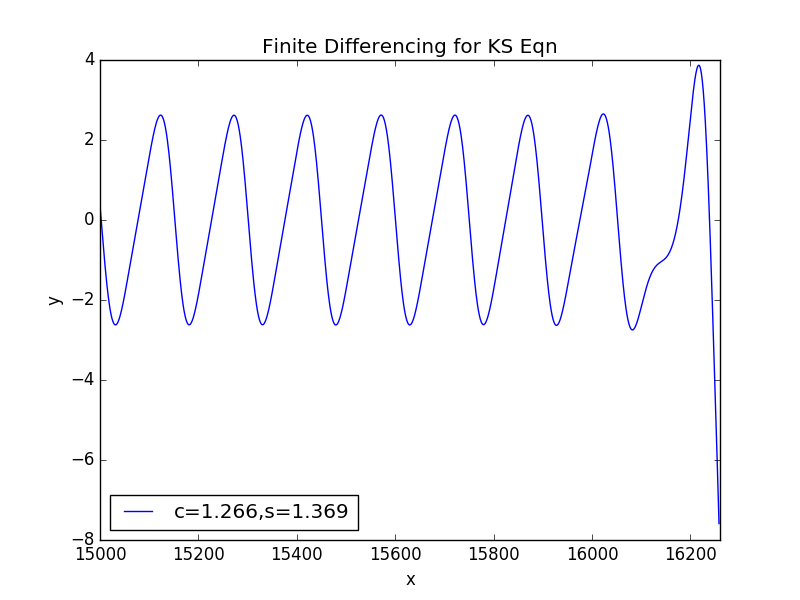
\includegraphics[scale=0.5]{ACxyplotc1266s1369a.png}
  \caption{
$(xy)$ plot. The trajectory generated through a finite difference scheme
outlined in Michelson\rf{Mks86} for $c=1.266$ and $s=1.369$.
  }

  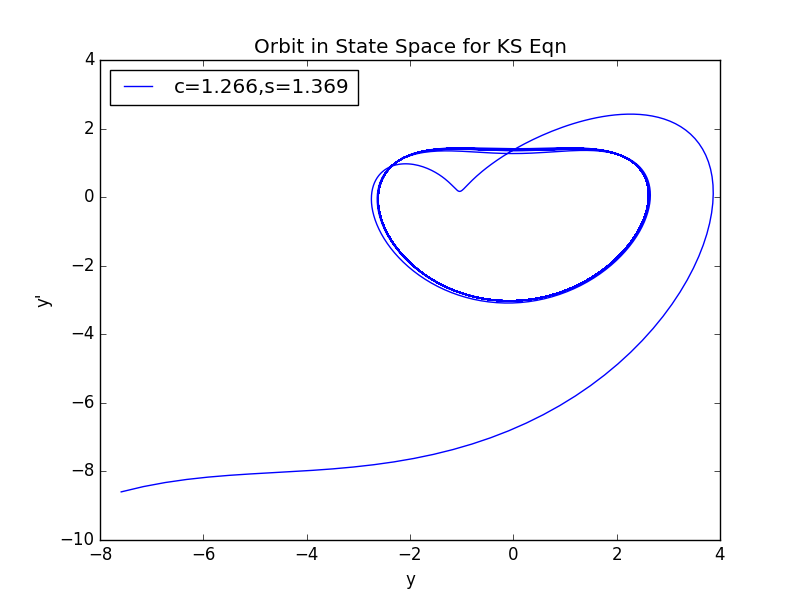
\includegraphics[scale=0.5]{ACorbitc1266s1369a.png}
  \caption{\Statesp\ plot. The near-periodic orbit generated through a finite difference
  scheme outlined in Michelson\rf{Mks86} for $c=1.266$ and $s=1.369$.}
\end{figure}
}


\item[2016-01-12 PC]  Literature
related to Michelson\rf{Mks86}:

Carmona \etal\rf{CFGT15}
{\em Noose structure and bifurcations of periodic orbits in reversible
three-dimensional piecewise linear differential systems}

Barker \etal\rf{BJNRZ12}
{\em Stability of periodic { Kuramoto-Sivashinsky} waves}

Aderogba, A. A. and Chapwanya, M. and Djoko\rf{AdChDj12}
{\em Travelling wave solution of the {Kuramoto-Sivashinsky} equation: A
computational study}


Dumortier,  Ibanez  and Kokubu\rf{DuIbKo06}
{\em Cocoon bifurcation in three-dimensional reversible vector fields}

Heidel and Zhang\rf{HeiZha07}
{\em Nonchaotic and chaotic behavior in three-dimensional quadratic systems:
{Five}-one conservative cases},

Nickel\rf{Nickel07}
{\em Travelling wave solutions to the {Kuramoto–Sivashinsky} equation }

Blomgren, Gasner, and Palacios\rf{BlGaPa05}
{\em Hopping behavior in the Kuramoto–Sivashinsky equation}
seems to be specific to $2D$: `` numerical `hopping' cellular flame
patterns are characterized by nonuniform rotations of a ring of cells, in
which individual cells make abrupt changes in their angular positions
while they rotate around the ring. Until now, these states have been
observed only in experiments but not in truly two-dimensional computer
simulations. A modal decomposition analysis of the simulated patterns,
via the proper orthogonal decomposition, reveals spatiotemporal behavior
in which the overall temporal dynamics is similar to that of equivalent
experimental states but the spatial dynamics exhibits a few more features
that are not seen in the experiments.
''


Dumortier,  Ibanez  and Kokubu\rf{DuIbKo06}
{\em Cocoon bifurcation in three-dimensional reversible vector fields}

Rempel \etal\rf{RCMR04}
{Analysis of chaotic saddles in high-dimensional dynamical systems: the
{Kuramoto-Sivashinsky} equation}: ``
study the role played by nonattracting chaotic sets called chaotic
saddles in chaotic transitions of high-dimensional dynamical systems. Our
methodology is applied to the Kuramoto-Sivashinsky equation. The paper
describes a novel technique that uses the stable manifold of a chaotic
saddle to characterize the homoclinic tangency responsible for an
interior crisis, a chaotic transition that results in the enlargement of
a chaotic attractor. The numerical techniques explained here are
important to improve the understanding of the connection between
low-dimensional chaotic systems and spatiotemporal systems which exhibit
temporal chaos and spatial coherence.''

Wilczak\rf{Wilczak03}
{\em Chaos in the {Kuramoto-Sivashinsky} equations -- a computer-assisted proof}

Strauss and Wang\rf{StrWan02}
 {\em Instability of traveling waves of the {Kuramoto-Sivashinsky} equation}

Ishimura\rf{Ishimura02}
{\em Remarks on third-order {ODEs} relevant to the {Kuramoto-Sivashinsky} equation}

Ishimura and Nakamura\rf{IshNak00}
{\em Nonexistence of monotonic solutions of some third-order ode relevant
to the {Kuramoto-Sivashinsky} equation}

Wittenberg and Holmes\rf{witt99hol}
{\em Scale and space localization in the {Kuramoto-Sivashinsky} equation}:
  ``
Using a wavelet basis, the spatiotemporally chaotic regime of the
    KSe is explored where a good seperation of scales is observed. In
    large scales, the dynamics is Gaussian. In the intermediate scales,
    the dynamics is reminiscent of travelling waves and heteroclinic
    cycles which is the typical behavior for small system size. In the
    small scales, the dynamics is intermittent. Through investigation
    of the interaction between different scales, we see the intermediate
    structures give the defining shape of the cell and the large scales
    trigger the spatiotemporal chaos. The small scales dissipate energy
    and modify the background in a average sense.

Yang\rf{ksyang97}
{\em On travelling-wave solutions of the {Kuramoto-Sivashinsky} equation}


Lau\rf{lau92}
{\em The cocoon bifurcations in three-dimensional systems with two fixed points}

Jones, Troy and MacGillivary\rf{kstroy92}
{\em Steady solutions of the {Kuramoto-Sivashinsky} equation for small wave speed}

Grimshaw and Hooper\rf{ksgrim91}
{\em The non-existence of a certain class of travelling wave solutions of
the {Kuramoto-Sivashinsky} equation},

Troy\rf{kstroy89}
{\em The existence of steady solutions of the {Kuramoto-Sivashinsky} equation}

Hooper and Grimshaw\rf{kshooper88}
{\em Travelling wave solutions of the {Kuramoto-Sivashinsky} equation}

Stanislavova and Stefanov\rf{StaSte11}
{\em Asymptotic estimates and stability analysis of {Kuramoto-Sivashinsky}
type models}

\end{description}

\subsection{Dong and Lan / DoLa14}
\label{sect:DoLa14}
Dong and Lan\rf{DoLa14}
{\em Organization of spatially periodic solutions of the steady
{Kuramoto-Sivashinsky} equation}

\begin{description}

\MNGpost{2017-07-17}{
{\bf DoLa14}
The goal of Dong and Lan\rf{DoLa14}
% {\em Organization of spatially
% periodic solutions of the steady {Kuramoto-Sivashinsky} equation}
is to
formulate a systematic way to locate periodic orbits with variational
method developed by Lan  and Cvitanovi{\'c}\rf{CvitLanCrete02,lanVar1},
as well as develop symbolic dynamics to classify these periodic orbits.
    }

\item[2013-12-29 PC] Dong and Lan\rf{DoLa14} study \eqva\ of \KS\ at $L
    = 43.5$. Previous system sizes were  was for antisymmetric
    subspace, system size $ \tildeL = 2.89109$ in
    \refref{Christiansen97}, $L = 38.5$ in \refref{lanCvit07}, $L =
    40.95$ in Lan~\etal\rf{LCC06}, and full \statesp\ $L=22$ in
    \refref{SCD07}. Dong and Lan continue the discussion of Lan's
    \HREF{http://www.cns.gatech.edu/~y-lan/thesis/thesis.pdf}
    {thesis}\rf{LanThesis}. Only \eqva, no mention of \reqva.

They credit Troy\rf{kstroy89,kstroy92} and Greene \& Kim\rf{ksgreene88}
with first studies of \KS\ \eqva.

\ACpost{2017-11-01}{{\bf DoLa14}
Reading this paper's introduction and background tremendously helped me understand
the \KSe\ more.
\begin{equation}
    u_t = (u^2)_x - u_{xx} - \nu u_{xxxx}
\end{equation}
The first derivative term is responsible for the interactions
between spatial modes at different scales (assuming this means length scales $L$)
and transfers energy from the low wavenumber modes to the higher ones. The second
term pumps energy into the system and makes it unstable at large scales while the
third term dissipates energy and damps at small scales.

Matt has gone over the spectral decomposition of the solution many times, but I
will just repeat it here for reference: using the form
\begin{equation}
    u(x,t) = i \sum_{k=-\infty}^{+\infty} a_k(t) e^{ikqx} \qquad \text{where } q = 2\pi/L,
\end{equation}
we can obtain an infinite ladder of coupled ODEs
\begin{equation}
    \dot{a}_k = [(kq)^2 - \nu (kq)^4] a_k - kq \sum_{m=-\infty}^{+\infty} a_m a_{k-m}.
\end{equation}
Since the dissipation term $\nu (kq)^4$ dominates for large wavenumber components, these
terms will not be excited enough significantly contribute to the dynamics. Thus, we can
truncate the set of ODEs such that $a_k = 0$ for $|k|>N$. In most cases, we take $N = 16$.
For small $L$, all Fourier modes are linearly stable, but the system quickly becomes
increasingly turbulent once $L$ increases by a significant amount.

From the video that Predrag recommended as well as the paper, the \KSe\ can be written as
\begin{align}
    &u^2 - u_x - \nu u_{xxx} = c\\
    &\implies \left\{
    \begin{array}{l}
	u_x = v\\
	v_x = w\\
	w_x = u^2 - v - c
    \end{array}
    \right.\\
    &\implies (u+w)_x = u^2 - c
\end{align}
We can see that $u+w$ increases without bound when $c<u^2$. When $c>u^2$ we can find
attractors appear in the state space. However, something weird happens when $c = u^2$
such that the derivative on the left side of Eqn 4.10 equals 0: both an attractor and
repeller appear in the state space, and it seems that trajectory enters the sink and
reappears at the source (if I'm understanding Predrag's drawing in the video correctly).

I'm still working through the variational methods part of the paper to see what they
actually did with the numerical simulations. So far, it seems that there exists four
simple building blocks for creating allowable orbits. This numbering notation reminds
me of the billiard (or pinball) orbit example that was covered in the Group Theory
class.
}

\item[2013-12-29 PC] we still have to study
Dong and Y. Lan\rf{DoLa14a}
{\em A variational approach to connecting orbits in nonlinear dynamical systems }

\end{description}

`` At fixed system size $L =43.5$, important equilibria
      are identified and shown to organize the dynamics. The first
      integral of the steady KSe leads to a 3D dynamical system with an
      integration constant $c$. At a typical value of $c = 0.40194$, four
      simplest cycles are identified and used as basic building blocks to
      construct longer cycles. The symbolic dynamics based on trajectory
      topology are very effective in classifying all short periodic
      orbits. The the return map on a chosen {\PoincSec} shows the
      complexity of the dynamics and the bifurcation of building blocks
      provides a chart to look for possible cycles at given periods. ''

The $n$ cell state\rf{FSTks86} is stable in finite windows for
arbitrarily large system sizes.

``
the antisymmetric heteroclinic orbit $\in \bbU^+$ connecting the two \eqva\ in
(9) is the only bounded nonconstant solution when the integration
constant $c\to\infty$\rf{mcord86}. For $c$ large enough, the heteroclinic
orbit remains the unique bounded solution\rf{Mks86}. It continues to be
numerically observable with $c$ down to 0.07\rf{kshooper88}, and was
computed analytically with normal form analysis for $c\ll
1$\rf{kschang86}. When $c$ decreases from large values, new connections
with more zeroes are born through saddle-node bifurcations until one
periodic orbit emerges as a limit of the connecting orbit with infinite
number of zeros. Bifurcation analysis with spatial Fourier modes gives
interesting features of spatially periodic steady solutions in certain
parameter regime\rf{ksgreene88}.
''

%%%%%%%%%%%%%%%%%%%%%%%%%%%%%%%%%%%%%%%%%%%%%%%%
%\printbibliography[heading=subbibintoc,title={References}]

The next benefit is not due to the inclusion of new methods but
rather the exclusion of old methods. Time integration and
recurrence functions based on pairwise distance have long been used in combination
to find initial conditions. % schatz/grigoriev, kerswell, viswanath.
In the high dimensional limit, both
of these components are time consuming. This is yet another
component of the dynamical systems formulation that gets worse
as spatial sizes increase. There are two detrimental factors
that contribute towards this. The number of dimensions must increase
in order to accurately resolve the domain. The other factor is that
the growth of complexity of solutions can reduce the number of recurrences
drastically. There isn't really a manner to deal with the increasing
number of computational variables other than to wait for improvements
in computing power and memory availability. As for the recurrences, the
typical solution for increasingly rare events is to compute in parallel when
possible. The exponential growth in complexity makes even this proposition
a daunting one.

% The italicized text captures my sentiment of this next paragraph.
The \spt\ completely avoids this by constructing larger \twots\
from the combination of smaller \twots. That is,
we locate the fundamental tiles, which are easy to find due to their small
domain size, and then build them up to create larger \twots. The only
search required is the search for the fundamental tiles. To stress
this even further \textit{one of the challenges of turbulence
computations has been eliminated}. The reason
why the search for the fundamental tiles is classified as ``easy'' is because
in the small domain size limit there just aren't that many \twots; the dynamics
is relatively simple.

% I'm trying to say that the arbitrary choice of norm is not as impactful in our case....
Recurrence functions also require the introduction of a norm,
typically chosen without taking the geometry of the state space into account.
Points that are close in this norm can be far apart in a dynamical sense (\ie, on opposite sides
of an unstable manifold). An arbitrary norm is also chosen in the \spt\
context but there are some subtle differences. For starters, the
norm introduced in the \spt\ formulation is not beholden to dynamics, as
there are no longer any dynamics to speak of.
Additionally, the norm in the \spt\ case measures the distance between \twots,
not just single state space points. This is not a statement of proof but rather
a suggestion that the underlying topology improves the reliability of
the chosen norm. Restated in a different manner, the \spt\ norm
takes both the magnitude and phase into account.

Conventional methods treat spatial dimensions
as finite and fixed; meanwhile, time is treated as infinite.
One interpretation is that this is natural due to the
human familiarity with finite space, especially in regards
to experimental setups.
This assumption is actually a very unnatural one
in the context of state space. The fundamental reason
for this is that it disregards
the translational invariance of the equations and while there
are implicit physical scales, choosing a specific domain size
to study is completely arbitrary. This notion
must be reconsidered going forward as it is a very strict constraint
on the space of solutions and on the study of turbulence in general.
Finite spatial dimensions of course have practical import, but
these specific constraints should only be imposed after the
study of infinite space-time, as they represent special
cases of the general equations. The \spt\ formulation handles
this properly by treating all continuous dimensions as equal
by respecting all translational symmetries.
What are the differences and advantages of this?
The first key difference is that the governing equation
dictates the \spt\ domain size in an unsupervised
fashion; the decision of what specific domain size
to study is no longer present in the discussion.
This is another manner in which
time and space are being treated as equals; the parameters $(L,T)$
that determine the size of the \spt\ domain are both allowed to vary.
The values of these parameters
are determined by the requirement that the equations
must be satisfied locally at every lattice site.
This small detail, allowing the domain size $L$ to vary,
is not as trivial as it seems. At present it has not been seen in
the dynamical systems literature. The variation of the period $T$ is
common, however. The likely culprit behind this different treatment
is likely a result of the equations themselves. This difficulty
is especially evident in the \KSe, whose spatial derivative terms
are of higher order than the first order time derivative, but also
there is a spatial derivative present in the nonlinear component.


    The conventional method to generate initial conditions
involves time integration and recurrence functions, the latter simply
calculates the pairwise distance between all points in a time integrated
series.%schatz/grigoriev, kerswell, viswanath.
In the high dimensional limit, both
of these components are time consuming. This is yet another
component of the dynamical systems formulation that gets worse
as spatial sizes increase. There are two detrimental factors
that contribute towards this. The number of dimensions must increase
in order to accurately resolve the domain. The other factor is that
the growth of complexity of solutions can reduce the number of recurrences
drastically. There isn't really a manner to deal with the increasing
number of computational variables other than to wait for improvements
in computing power and memory availability. As for the recurrences, the
typical solution for increasingly rare events is to compute in parallel when
possible. The exponential growth in complexity makes even this proposition
a daunting one.

The \spt\ completely avoids this by constructing larger \twots\
from the combination of smaller \twots. That is,
we locate the fundamental tiles, which are easy to find due to their small
domain size, and then build them up to create larger \twots. The only
search required is the search for the fundamental tiles. To stress
this even further \textit{one of the challenges of turbulence
computations has been eliminated}. The reason
why the search for the fundamental tiles is classified as ``easy'' is because
in the small domain size limit there just aren't that many \twots; the dynamics
is relatively simple.

Recurrence functions also require the introduction of a norm,
typically chosen without taking the geometry of the state space into account.
Points that are close in this norm can be far apart in a dynamical sense (\ie, on opposite sides
of an unstable manifold). An arbitrary norm is also chosen in the \spt\
context but there are some subtle differences. For starters, the
norm introduced in the \spt\ formulation is not beholden to dynamics, as
there are no longer any dynamics to speak of.
Additionally, the norm in the \spt\ case measures the distance between \twots,
not just single state space points. This is not a statement of proof but rather
a suggestion that the underlying topology improves the reliability of
the chosen norm. Restated in a different manner, the \spt\ norm
takes both the magnitude and phase into account.
Another numerical advantage is that the \spt\ formulation is able to find solutions
of the \KSe\ starting from modulated random noise. The specifics
of ``modulated random noise'' are described in the numerical methods section
but it can essentially be thought of as randomly assigning values to \spt\
Fourier modes. The ability to find solutions from this starting point
is a radical improvement over the conventional capabilities. This is of course
in conjunction with allowing the \spt\ domain to change. The reaction to these
changes individually has induced skepticism and disbelief; together they comprise
a completely unheard of force.

The \spt\ formulation also includes the improvement of a commonly
practiced numerical method known as pseudo-arclength continuation.
The general idea is to track a solution as a parameter is varied. In the
Navier-Stokes equations this is typically the Reynolds number.
The improvement is due to our common refrain: the lack of dynamical
instability and the topological constraint of \twots. There can
be more confidence that if the continuation fails it is due to the solution
not existing rather than not being able to converge due to dynamical instability.

\section{\KSe}
% KSe.tex
% $Author: siminos $ $Date: 2009-10-05 16:13:22 -0400 (Mon, 05 Oct 2009) $

\section{\KSe}
\label{s-KS}

The \KS\ [henceforth KS] system\rf{ku,siv},
which arises in the description of
stability of flame fronts, reaction-diffusion systems and many other
physical settings\rf{KNSks90}, is one of the simplest nonlinear PDEs that
exhibit spatiotemporally chaotic behavior. In the formulation
adopted here, the time evolution of the `flame front velocity'
$u=u(x,t)$ on a periodic domain $u(x,t) = u(x+L,t)$ is given by
\beq
  u_t = F(u) = -{\textstyle\frac{1}{2}}(u^2)_x-u_{xx}-u_{xxxx}
    \,,\qquad   x \in [-L/2,L/2]
    \,.
\ee{ks}
Here $t \geq 0$ is the time, and $x$ is the spatial coordinate.
The subscripts $x$ and $t$ denote partial derivatives with respect to
$x$ and $t$. In what follows
we shall state results of all calculations either in units of the
`dimensionless system size' $\tildeL$, or the system size $L = 2 \pi
\tildeL$. \refFig{f:ks_largeL} presents a typical `turbulent' evolution
for KS. All numerical results presented in this paper
are for the system size $\tildeL=22/2\pi = 3.5014\ldots$, for which a
structurally stable chaotic attractor is observed (see \reffig{f:ks_L22}).
Spatial periodicity $u(x,t)=u(x+L,t)$
makes it convenient to work in the Fourier space,
\beq
  u(x,t)=\sum_{k=-\infty}^{+\infty} a_k (t) e^{ i k x /\tildeL }
\,,
\ee{eq:ksexp}
with the $1$-dimensional PDE \refeq{ks}
replaced by an infinite set of
ODEs for the complex Fourier coefficients $a_k(t)$:
\beq
\dot{a}_k= \pVeloc_k(a)
     = ( q_k^2 - q_k^4 )\, a_k
    - i \frac{q_k}{2} \sum_{m=-\infty}^{+\infty} a_m a_{k-m}
\,,
\ee{expan}
where $q_k = k/\tildeL$.
Since $u(x,t)$ is real, $a_k=a_{-k}^\ast$, and we can replace the
sum by an $m > 0$ sum.

Due to the hyperviscous damping $u_{xxxx}$, long time solutions of KS
equation are smooth, $a_k$ drop off fast
with $k$, and truncations of \refeq{expan} to $16 \leq N \leq 128$
terms yield accurate solutions for system sizes considered here (see
\refappe{sec:fourierRLD}).  Robustness of the long-time dynamics
of KS as a function of the number of Fourier modes kept in truncations
of \refeq{expan} is, however, a subtle issue.  Adding an extra mode to
a truncation of the system introduces a small perturbation in the
space of dynamical systems.  However, due to the lack of structural
stability both as a function of truncation $N$, and the system size
$L$, a small variation in a system parameter can (and often will)
throw the dynamics into a different asymptotic state.  For example,
asymptotic attractor which appears to be chaotic in a $N$-dimensional
\statesp\ truncation can collapse into an attractive cycle
for $(N\!+\!1)$-dimensions.
Therefore, the selection of parameter $L$ for which a
structurally stable chaotic dynamics exists and can be
studied is rather subtle. We have found that the value of $L
= 22$ studied in \refsect{sec:L22} satisfies these
requirements. In particular, all of the equilibria and
relative equilibria persist and remain unstable when $N$ is
increased from 32 (the value we use in our numerical
investigations) to 64 and 128.  Nearly all of the \rpo s we
have found for this system also exist and remain unstable for
larger values of $N$ as well as smaller values of the
integration step size (see \refappe{sec:lmderRLD} for
details).

%%%%%%%%%%%%%%%%%%%%%%%%%%%%%%%%%%%%%%%%%%%%%%%%%%%%%%%%%%%%%%
\begin{figure}[t]
\begin{center}
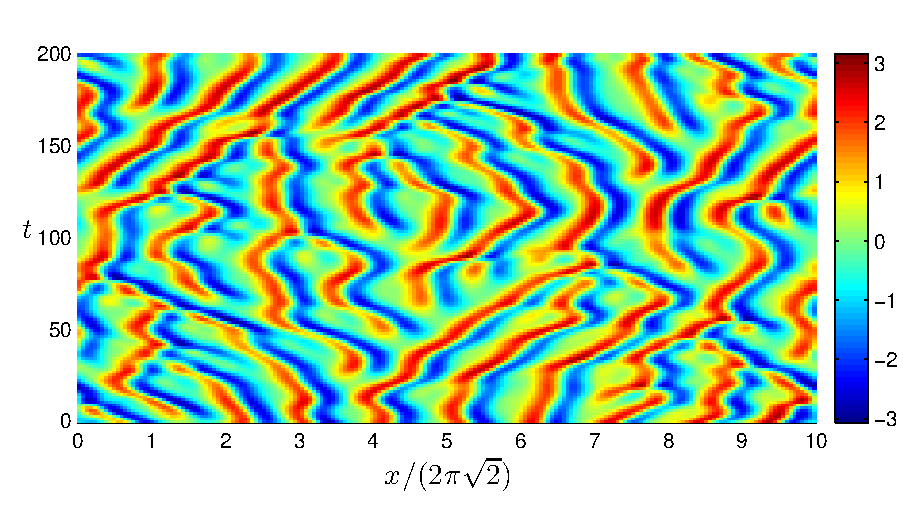
\includegraphics[width=0.9\textwidth]{figs_bmp/ks_largeL_cbar_200.eps} 
\end{center}
\caption{
A typical spatiotemporally chaotic solution of the \KSe, system size
$L=20\pi\sqrt{2}\approx 88.86$.  The $x$ coordinate is scaled
with the most unstable wavelength $2\pi\sqrt{2}$, which is
approximately also the mean wavelength of the turbulent flow.
The color bar indicates the color scheme for $u(x,t)$, used also
for the subsequent figures of this type.
     } \label{f:ks_largeL}
\end{figure}
%%%%%%%%%%%%%%%%%%%%%%%%%%%%%%%%%%%%%%%%%%%%%%%%%%%%%%%%%%%%%%%%%%

\subsection{Symmetries of \KSe}
\label{sec:KSeSymm}

The KS equation is Galilean invariant: if $u(x,t)$ is a solution,
then $u(x -ct,t) -c $, with $c$ an arbitrary constant
speed, is also a solution. Without loss of generality, in our
calculations we shall set the mean velocity of the front to zero,
\beq \int dx \, u = 0 \,. \ee{GalInv}
As $\dot{a_0}=0$ in
\refeq{expan}, $a_0$ is a conserved quantity
fixed to $a_0=0$ by the condition \refeq{GalInv}. $G$, the group of actions $ g \in G $ on a
\statesp\ (reflections, translations, \etc) is a symmetry of the KS
flow \refeq{ks} if $g\,u_t = F(g\,u)$.
The KS equation is time translationally invariant, and space translationally invariant
on a periodic domain under
the 1-parameter group of
$O(2): \{\Shift_{\shift/L},\Refl \}$.
If $u(x,t)$ is a solution, then
$\Shift_{\shift/L}\, u(x,t) = u(x+\shift,t)$
is an equivalent solution for any shift
$-L/2 < \shift \leq L/2$,
as is the
reflection (`parity' or `inversion')
\beq
    \Refl \, u(x) = -u(-x)
\,.
\ee{KSparity}
The translation operator action on the Fourier coefficients \refeq{eq:ksexp},
represented here by a complex valued vector
$a = \{a_k\in\mathbb{C}\,|\,k = 1, 2, \ldots\}$, is given by
\beq
  \Shift_{\shift/L}\, a = \mathbf{g}(\shift) \, a \,,
  \label{eq:shiftFour}
\eeq
where $\mathbf{g}(\shift) = \diag( e^{i q_k\, \shift} )$ is a complex
valued diagonal matrix, which amounts to the $k$-th mode complex plane
rotation by an angle $k\, \shift /\tildeL$.  The reflection acts on
the Fourier coefficients by complex conjugation,
\beq
  \Refl \, a = -a^\ast
\,.
\ee{FModInvSymm}
Reflection generates the dihedral subgroup $D_1 = \{1, \Refl\}$
of $O(2)$.  Let $\bbU$ be the space of
real-valued velocity fields periodic and square integrable
on the interval $\Omega = [-L/2,L/2]$,
\begin{align}
 \bbU  &= \{u \in L^2(\Omega) \; | \; u(x) = u(x+L)\}  \,.
\end{align}
A continuous symmetry maps each state $u \in \bbU$
to a manifold of functions with identical dynamic behavior.
Relation $\Refl^2 = 1$ induces linear decomposition
$u(x) = u^+(x)+ u^-(x)$,
$u^\pm(x)= P^\pm u(x) \in  \bbU^\pm$,
into irreducible subspaces
$
\bbU = \bbU^+
       \oplus \bbU^-
$, where
\beq
    P^+=(1+\Refl)/2
    \,,\qquad
    P^-=(1-\Refl)/2
\,,
\ee{P1P2proj} are the antisymmetric/symmetric projection operators.
Applying $P^+,\,P^-$ on the KS equation \refeq{ks} we have\rf{KNSks90}
\bea
 u_t^+ &=& - (u^+u^+_x + u^-u^-_x )
                - u^+_{xx} - u^+_{xxxx}
    \continue
 u_t^- &=& - (u^+u^-_x + u^-u^+_x )
                - u^-_{xx} - u^-_{xxxx}
\,.
\label{KSD1}
\eea
If $u^- = 0$, KS flow is confined to
the antisymmetric $\bbU^+$ subspace,
\beq
 u_t^+ = - u^+u^+_x
                - u^+_{xx} - u^+_{xxxx}
\,,
\label{KSU+}
\eeq
but otherwise the nonlinear terms in \refeq{KSD1}
mix the two subspaces.

Any rational shift $ \Shift_{1/m}u(x)=u(x+L/m)$ generates a discrete
cyclic subgroup $C_m$ of $O(2)$, also a symmetry of KS
system. Reflection together with $C_m$ generates another
symmetry of KS system, the dihedral subgroup $D_m$ of $O(2)$.
The only non-zero Fourier components of a solution invariant
under $C_m$ are $a_{jm} \neq 0$, $j =1,2,\cdots$, while for a
solution invariant under $D_m$ we also have the condition
$\Re a_j=0$ for all $j$.
$D_m$ reduces the dimensionality of \statesp\ and aids computation of
\eqva\ and \po s within it. For example, the 1/2-cell translations \beq
    \Shift_{1/2}\, u(x)=u(x+L/2)
\ee{KSshift}
and reflections generate $O(2)$
subgroup $D_2 = \{1, \Refl,\Shift,\Shift\Refl\}$,
which
reduces the \statesp\ into four irreducible subspaces
(for brevity, here $\Shift = \Shift_{1/2}$):
\begin{align}
 & \qquad\qquad\qquad\qquad\qquad
              ~~~ \Shift ~~ \Refl  ~\;  \Shift\Refl
    \nnu\\
P^{(1)} &= \frac{1}{4} (1 + \Shift + \Refl + \Shift\Refl)
           ~~~~  S  ~~  S   ~~   S
    \nnu\\
P^{(2)} &= \frac{1}{4} (1 + \Shift - \Refl - \Shift\Refl)
            ~~~~  S  ~~  A   ~~   A
    \nnu\\
P^{(3)} &= \frac{1}{4} (1 - \Shift + \Refl - \Shift\Refl)
           ~~~~  A  ~~  S   ~~   A
     \label{ek_defn}\\
P^{(4)} &= \frac{1}{4} (1 - \Shift - \Refl + \Shift\Refl)
          ~~~~  A  ~~  A   ~~   S
\,.
    \nnu
\end{align}
$P^{(j)}$ is the projection operator onto
$u^{(j)}$ irreducible subspace, and the last 3 columns
refer to the symmetry (or antisymmetry) of
$u^{(j)}$ functions under reflection and
1/2-cell shift.
By the same argument that identified \refeq{KSU+} as
the invariant subspace of KS, here the KS flow
stays within the
 $\bbU^S =  \bbU^{(1)}+ \bbU^{(2)}$
irreducible $D_1$ subspace of
$u$ profiles symmetric under 1/2-cell shifts.

While in general the bilinear term $(u^2)_x$  mixes the
irreducible subspaces of $D_n$, for $D_2$ there are
four subspaces invariant under the flow\rf{KNSks90}:
\begin{romannum}
 \item[$\{0\}$:~~~~~~] the $u(x)=0$ {\eqv}
 \item[$\bbU^+ = \bbU^{(1)}+ \bbU^{(3)} $:]
    the reflection $D_1$ irreducible space of antisymmetric $u(x)$
 \item[$\bbU^S =  \bbU^{(1)}+ \bbU^{(2)}$:]
    the shift $D_1$ irreducible space of $L/2$ shift symmetric  $u(x)$
 \item[$\bbU^{(1)}$:~~~~~]
    the $D_2$ irreducible  space of $u(x)$ invariant under $x\mapsto L/2-x,\ u\mapsto -u$.
\end{romannum}
With the continuous
translational symmetry eliminated within each subspace, there are no
\reqva\ and \rpo s, and one
can focus on the \eqva\ and \po s only, as was done
for $\bbU^+$ in \refrefs{Christiansen97,LanThesis,lanCvit07}.
In the Fourier
representation, the
$u \in \bbU^+$
antisymmetry amounts to having purely imaginary
coefficients, since $a_{-k}= a^\ast_k = -a_k$.
The 1/2 cell-size shift $\Shift_{1/2}$
generated 2-element discrete subgroup
$\{1,\Shift_{1/2}\}$ is
of particular interest
because in the $\bbU^+$ subspace the translational invariance of the full system reduces to
invariance under discrete translation \refeq{KSshift} by half a
spatial period $L/2$.

Each of the above dynamically invariant subspaces is unstable
under small perturbations, and generic solutions of \KSe\ belong to
the full space.
Nevertheless, since  all \eqva\ of the KS flow studied in this paper
lie in the $\bbU^+$ subspace (see
\refsect{sec:L22}), $\bbU^+$  plays important role for the global
geometry of the flow.
The linear stability matrices of these \eqva\ have
eigenvectors both in and outside of $\bbU^+$, and need to be
computed in the full \statesp.




\subsection{\Eqva\ and \reqva}
\label{sec:stks}

\Eqva\  (or the steady solutions)
are the fixed profile time-invariant solutions,
\beq
 u(x,t) = u_\stagn(x)
\,.
\ee{eqva}
Due to the translational symmetry,
the KS system also allows for
\reqva\ (traveling waves, rotating waves),
characterized by a fixed profile $u_\stagn(x)$
moving with constant speed $c$, {\ie}
\beq
 u(x,t) =  u_\stagn(x-ct)
\,.
\ee{reqva}
Here suffix ${}_\stagn$ labels a particular invariant solution.
Because of the reflection symmetry \refeq{KSparity},
the \reqva\ come in counter-traveling pairs
$u_\stagn(x-ct)$, $-u_\stagn(-x+ct)$.

The \reqv\ condition for the {\KS} PDE \refeq{ks}
is the ODE
\beq
{\textstyle\frac{1}{2}}(u^2)_x+u_{xx}+ u_{xxxx}=c \, u_x
\ee{KSeqvCond}
which can be analyzed as a dynamical system in its own right.
Integrating once we get
\beq
{\textstyle\frac{1}{2}}u^2 - c u + u_x + u_{xxx}=\expctE
\,.
\label{eq:stdks}
\eeq
This equation can be interpreted as a 3-dimen\-si\-on\-al dynamical system
with spatial coordinate $x$ playing the role of `time,'
and the integration constant \expctE\ can be interpreted as `energy,'
see \refsect{sec:energy}.

For $\expctE>0$ there is rich $\expctE$-dependent dynamics,
with fractal sets of bounded solutions investigated in depth
by Michelson\rf{Mks86}. For $\tildeL<1$ the only \eqv\ of the
system is the globally attracting constant solution
$u(x,t)=0$, denoted $\EQV{0}$ from now on. With increasing
system size $L$ the system undergoes a series of
bifurcations. The resulting \eqva\ and \reqva\ are described
in the classical papers of Kevrekidis, Nicolaenko and
Scovel\rf{KNSks90}, and Greene and Kim\rf{ksgreene88},
among others. The relevant bifurcations up to the
system size investigated here are summarized in
\reffig{fig:ksBifDiag}: at $\tildeL=22/2\pi = 3.5014\cdots$,
the {\eqva} are the constant solution \EQV{0},
the  \eqv\ \EQV{1} called GLMRT by Greene and
Kim\rf{laquey74,ksgreene88},
the $2$- and $3$-cell states
\EQV{2} and \EQV{3}, and the pairs of \reqva\ \REQV{\pm}{1},
\REQV{\pm}{2}.
All \eqva\ are in the antisymmetric subspace $\bbU^+$, while
\EQV{2} is also invariant under $D_2$ and \EQV{3} under
$D_3$.


%%%%%%%%%%%%%%%%%%%%%%%%%%%%%%%%%%%%%%%%%%%%%%%%%%%%%%%%%%%%%%%%
\begin{figure}[t]       \label{fig:ksBifDiag}
\begin{center}
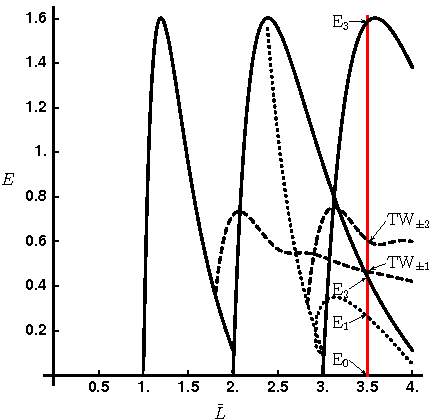
\includegraphics[width=0.5\textwidth]{figs_bmp/ksBifDiag_pst.eps}
\end{center}
\caption{
The energy \refeq{ksEnergy} of the \eqva\ and \reqva\ that
exist up to $L=22$, $\tildeL = 3.5014\ldots$, plotted as a function
of the system size $\tildeL = L/2\pi$ (additional \eqva, not present
at $L = 22$ are given in \refref{ksgreene88}). Solid curves denote
$n$-cell solutions \EQV{2} and \EQV{3}, dotted curves the GLMRT
\eqv\ \EQV{1},
and dashed curves the \reqva\ \REQV{\pm}{1} and \REQV{\pm}{2}.
The parameter $\alpha$ of \refrefs{KNSks90,ksgreene88} is
related to the system size by $\tildeL=\sqrt{\alpha/4}$.
        }
\end{figure}
%%%%%%%%%%%%%%%%%%%%%%%%%%%%%%%%%%%%%%%%%%%%%%%%%%%%%%%%%%%%%%%%%%

In the Fourier representation the \reqva\ time dependence is
\beq
 a_k(t) e^{-itc q_k} = a_k(0)
\,.
\ee{reqvaF}
Differentiating with respect to time, we obtain
the Fourier space version of the \reqv\ condition
\refeq{KSeqvCond},
\beq
 \pVeloc_k(a) - i q_k \velRel a_k = 0
\,,
\ee{reqvCondF}
which we solve for (time independent) $a_k$ and $c$.
Periods of spatially periodic {\eqva} are $L/n$ with integer $n$.
Every time the system size crosses  $\tildeL=n$,
$n$-cell states
are generated through pitchfork bifurcations off $u =0$
equilibrium.
Due to the translational invariance of {\KSe},
they form invariant circles
in the full \statesp.
In the $\bbU^+$ subspace considered here,
they correspond to $2n$ points, each shifted by $L/2n$.
For a sufficiently small $L$
the number of {\eqva} is small and
concentrated on the low wave-number end of the Fourier spectrum.

In a periodic box of size $L$
both \eqva\ and \reqva\ are  periodic solutions
embedded in 3-$d$ space, conveniently represented as loops in
$(u,u_x,u_{xx})$ space, see \reffig{f:KS22Equil}\,(\textit{d}).
In this representation the continuous translation symmetry
is automatic -- a rotation in the $[0,L]$ periodic domain only
moves the points along the loop. For an \eqv\ the points
are stationary in time; for \reqv\ they move in time, but in
either case, the loop remains invariant.
So we do not have the problem that we encounter in the Fourier
representation, where seen from the frame of one of the \eqva\
the rest trace out circles under the action of continuous symmetry
translations.

From \refeq{expan} we see that the origin $u(x,t) = 0$
has Fourier modes as the linear stability eigenvectors
(see \refappe{sec:stability}).  The $|k|<\tildeL$
long wavelength perturbations of the flat-front {\eqv}
are linearly unstable, while for
$|k|$ sufficiently larger than $\tildeL$ the short wavelength
perturbations are strongly contractive. The high $k$
eigenvalues, corresponding to rapid variations of the flame
front, decay so fast that the corresponding eigendirections
are physically irrelevant. Indeed, \refref{YaTaGiChRa08} shows that
the chaotic solutions of spatially extended dissipative
systems evolve within an inertial manifold spanned by a
finite number of physical modes, hyperbolically isolated from
a set of residual degrees of freedom with high $k$, themselves individually
isolated from each other.
The most unstable mode, nearest to $|k|=\tildeL/\sqrt{2}$,
sets the scale of the mean wavelength $\sqrt{2}$
of the KS `turbulent' dynamics,
see \reffig{f:ks_largeL}.


\subsection{\Rpo s, symmetries and \po s} \label{sec:KSePO}

The KS equation \refeq{ks} is time translationally invariant, and
space translationally invariant under the 1-$d$ Lie group of $O(2)$
rotations: if $u(x,t)$ is a solution, then $u(x+\shift,t)$ and
$-u(-x,t)$ are equivalent solutions for any $-L/2 < \shift \leq
L/2$.
As a result of invariance under $\Shift_{\shift/L}$,
KS equation can have \rpo\ solutions
with a profile $u_p(x)$, period $\period{p}$, and a
nonzero shift $\shift_p$
\beq
  \Shift_{\shift_p/L}u(x,\period{p}) =
  u(x+\shift_p,\period{p}) = u(x,0) = u_p(x)\,.
\label{KSrpos}
\eeq
{\Rpo s} \refeq{KSrpos} are periodic in
$\velRel_p=\shift_p/\period{p}$ co-rotating frame (see
\reffig{f:MeanVelocityFrame}), but in the stationary frame their
trajectories are quasiperiodic.  Due to the reflection symmetry
\refeq{KSparity} of KS equation, every {\rpo} $u_p(x)$ with shift
$\shift_p$ has a symmetric partner $-u_p(-x)$ with shift $-\shift_p$.

Due to invariance under reflections, KS equation can also have
\rpo s {\em with reflection}, which are
characterized by a profile $u_p(x)$ and
period $\period{p}$
\beq
  \Refl u(x+\shift,\period{p}) =
  -u(-x-\shift,\period{p}) = u(x+\shift,0) = u_p(x)
  \,,
\label{KSpos}
\eeq
giving the family of equivalent solutions
parameterized by $\shift$
(as the choice of the reflection point is arbitrary,
the shift can take any value in $-L/2 < \shift \leq L/2$).

Armbruster \etal\rf{AGHks89,AGHO288} and Brown and
Kevrekidis\rf{BrKevr96} (see also \refref{Krupa90}) link the
birth of \rpo s to an infinite period global bifurcation
involving a heteroclinic loop connecting equilibria or a
bifurcation of \reqva, and also report creation of \rpo\
branches through bifurcation of \po s.

As $\shift$ is continuous in the interval $[-L/2, L/2]$,
the likelihood of a \rpo\ with $\shift_p = 0$ shift is zero,
unless an exact periodicity is enforced by a discrete symmetry,
such as the dihedral symmetries discussed above.
If the shift $\shift_p$ of a \rpo\ with period $\period{p}$ is such
that $\shift_p /L$ is a rational number, then the orbit is
periodic with period $n\period{p}$.  The likelihood to find such \po s is
also zero.

However, due to the KS equation invariance under
the dihedral $D_n$ and cyclic $C_n$ subgroups, the following
types of \po s are possible:

{\bf (a)} The \po\ lies
within a subspace pointwise invariant under the action of
$D_n$ or $C_n$. For instance, for $D_1$ this is the
$\bbU^+$ antisymmetric subspace, $-u_p(-x) = u_p(x)$, and
$u(x,\period{p}) = u(x,0) = u_p(x)$. The periodic orbits
found in \refrefs{Christiansen97,lanCvit07} are
all in $\bbU^+$, as the dynamics is restricted to
antisymmetric subspace. For $L=22$ the dynamics in $\bbU^+$
is dominated by attracting (within the subspace)
heteroclinic connections and thus we have no periodic orbits
of this type, or in any other of the $D_n$--invariant
subspaces, see \refsect{sec:L22}.

{\bf (b)} The \po\ satisfies
\beq
	 u(x,t+\period{p})=\gamma u(x,t)\,,
	\label{eq:POspattemp}
\eeq
for some group element $\gamma\in O(2)$ such that
$\gamma^m=e$ for some integer $m$ so that the orbit repeats
after time $m \period{p}$ (see
\refref{golubitsky2002sp} for a general discussion of
conditions on the symmetry of a \po).
If an orbit is of reflection type \refeq{KSpos},
$\Refl\Shift_{\shift/L} u(x,\period{p}) =
-u(-x-\shift,\period{p}) = u(x,0)$, then it is pre-periodic
to a \po\ with period $2\period{p}$. Indeed, since
$(\Refl\Shift_{\shift/L})^2 = \Refl^2 = 1$, and the KS
solutions are time translation invariant, it follows from
\refeq{KSpos} that
\[
  u(x,2\period{p}) = \Refl\Shift_{\shift/L} u(x,\period{p}) =
  (\Refl\Shift_{\shift/L})^2 u(x,0) = u(x,0)\;.
\]
Thus any shift acquired during time $0$ to
$\period{p}$ is compensated by the opposite shift during
evolution from $\period{p}$ to $2 \period{p}$.
All periodic orbits we have found for $L=22$ are of type
\refeq{eq:POspattemp} with $\gamma=R$. Pre-periodic orbits
with $\gamma\in C_n$ have been found by Brown and
Kevrekidis\rf{BrKevr96} for KS system sizes larger than ours,
but we have not found any for $L=22$.
Pre-periodic orbits are a hallmark of any dynamical system
with a discrete symmetry, where they have a natural
interpretation as \po s in the fundamental
domain\rf{CvitaEckardt,DasBuch}.

\section{Energy transfer rates}
\label{sec:energy}

In physical settings where the observation times are much
longer than the dynamical `turnover' and Lyapunov times
(statistical mechanics, quantum physics, turbulence) periodic
orbit theory\rf{DasBuch} provides highly accurate predictions
of measurable long-time averages such as the dissipation and
the turbulent drag\rf{GHCW07}. Physical predictions have to
be independent of a particular choice of ODE representation
of the PDE under consideration and, most importantly,
invariant under all symmetries of the dynamics. In this
section we discuss a set of such physical observables for the
1-$d$ KS invariant under reflections and translations. They
offer a representation of dynamics in which the symmetries
are explicitly quotiented out. We shall use these
observables in \refsect{sec:energyL22} in order to
visualize a set of solutions on these coordinates.

The {space average} of a function $\obser = \obser(\pSpace,t) = \obser(u(x,t))$  on
the interval $L$,
\beq
    \expct{\obser} = \Lint{\pSpace}\, \obser(\pSpace,t)
    \,,
    \label{rpo:spac_ave}
\eeq
is in general time dependent.
Its mean value is given by the {time average}
\beq
\timeAver{\obser}
    =
\lim_{t\rightarrow \infty} \frac{1}{t} \int_0^t \! d\tau \, \expct{\obser}
    =
\lim_{t\rightarrow \infty} \frac{1}{t} \int_0^t \!
    \Lint{\tau}  d\pSpace\, \obser(\pSpace,\tau)
    \,.
\label{rpo:tim_ave}
\eeq
The mean value of $\obser = \obser(u_\stagn) \equiv \obser_\stagn$ evaluated on
\eqv\ or {\reqv} $u(\pSpace,t) = u_\stagn(\pSpace-ct)$, labeled by  $q$ as in 
\refeq{reqva}, is
\beq
\timeAver{\obser}_\stagn = \expct{\obser}_\stagn = \obser_\stagn\,.
\label{rpo:u-eqv} \eeq 
Evaluation of the infinite time average
\refeq{rpo:tim_ave} on a function of a \po\ or \rpo\
$u_p(\pSpace,t)=u_p(\pSpace+\shift_p,t+\period{p})$ requires only a single
$\period{p}$ traversal,
\beq
  \timeAver{\obser}_p = \frac{1}{\period{p}}
    \int_0^{\period{p}} \! d\tau \, \expct{\obser}
\,.
\label{rpo:u-cyc}
\eeq

Equation \refeq{ks} can be written as
\beq
    u_t=- V_x
        \,,\qquad
    V(x,t)={\textstyle\frac{1}{2}}u^2+u_{x} + u_{xxx}
    \,.
\ee{ksPotent}
If $u$ is `flame-front velocity' then \expctE, defined in
\refeq{eq:stdks}, can be interpreted as the mean energy
density. So, even though KS is a phenomenological
small-amplitude equation, the time-dependent $L^2$ norm
of $u$,
\beq
    \expctE=
  \Lint{\pSpace}
  V(x,t)=
  \Lint{\pSpace} \frac{u^2}{2}
  \,,
  \label{ksEnergy}
\eeq
has a physical interpretation\rf{ksgreene88} as the average `energy'
density of the flame front. This analogy to the mean kinetic energy
density for the Navier-Stokes motivates what follows.

The energy \refeq{ksEnergy} is intrinsic to the flow,
independent of the particular ODE basis set chosen to
represent the PDE. However, as the Fourier amplitudes are
eigenvectors of the translation operator, in the Fourier
space the energy is a diagonalized quadratic norm,
\beq
\expctE
          =  \sum_{k=-\infty}^{\infty} E_k
\,,\qquad
E_k =
    {\textstyle\frac{1}{2}}|a_k|^2
\,,
\ee{EFourier}
and explicitly invariant term by term
under translations
\refeq{eq:shiftFour}
and reflections \refeq{KSparity}.

Take time derivative of the energy density \refeq{ksEnergy},
substitute \refeq{ks} and integrate by parts. Total derivatives vanish
by the spatial periodicity on the $L$ domain:
\bea
   \dot{\expctE} &=&
     \expct{u_t \, u}
         = - \expct{\left({u^2}/{2} + u_{x} + u_{xxx}\right)_x u }
    \continue
    &=&
\expct{ u_x \, {u^2}/{2} + u_{x}^2 + u_x \, u_{xxx}}
    \,.
\label{rpo:ksErate}
\eea
The first term in \refeq{rpo:ksErate} vanishes by
integration by parts,
\(
3 \expct{ u_x \, u^2}= \expct{(u^3)_x} = 0
\,,
\)
and integrating the third term by parts yet again
one gets\rf{ksgreene88} that the energy variation
\beq
   \dot{\expctE} = P - D
                \,,\qquad
      P =  \expct{u_{x}^2}
                \,,\quad
      D =  \expct{u_{xx}^2}
\ee{EnRate}
balances the power $P$ pumped in by anti-diffusion $u_{xx}$
against the energy dissipation rate $D$
by hyper-viscosity $u_{xxxx}$
in the KS equation \refeq{ks}.

The time averaged energy density  $\timeAver{E}$
computed on a typical orbit goes to a constant, so
the mean values \refeq{rpo:tim_ave} of drive and dissipation
exactly balance each other:
\beq
    \timeAver{\dot{E}}  =
    \lim_{t\rightarrow \infty}
        \frac{1}{t} \int_0^t d\tau \, \dot{\expctE}
=
      \timeAver{P} - \timeAver{D}
= 0
    \,.
\ee{rpo:EtimAve}
In particular, the \eqva\
and \reqva\ fall onto the diagonal in \reffig{f:drivedrag}\,(\textit{a}),
and so do time averages computed on \po s and \rpo s:
\beq
\timeAver{E}_p =
\frac{1}{\period{p}} \int_0^\period{p}d\tau \, E(\tau)
    \,,\qquad
\timeAver{P}_p =
\frac{1}{\period{p}} \int_0^\period{p} d\tau \, P(\tau)
    =
      \timeAver{D}_p
    \,.
\label{poE}
\eeq
In the Fourier basis \refeq{EFourier} the conservation of energy on average
takes form
\beq
0 = \sum_{k=-\infty}^{\infty} ( q_k^2 - q_k^4 )\,
    \timeAver{E}_k
\,,\qquad
E_k(t) =  {\textstyle\frac{1}{2}} |a_k(t)|^2
\,.
\ee{EFourier1}
The large $k$ convergence of this series is insensitive to the
system size $L$; $\timeAver{E_k}$ have to decrease much faster than
$q_k^{-4}$.
Deviation of $E_k$ from this bound for small $k$ determines the active modes.
For \eqva\ an $L$-independent bound
    on $E$ is given by Michelson\rf{Mks86}.
The best current bound\rf{GiacoOtto05,bronski2005} on the long-time limit
of $E$
as a function of the system size $L$ scales as
$E \propto L^2$.

\section{Spatial integration}
% siminos/gudorf/thesis/chapter/KStimeInt.tex
% $Author: predrag $ $Date: 2020-05-25 15:18:45 -0400 (Mon, 25 May 2020) $

%\section{Spatially periodic \KS}
%\label{sect:KStimeInt}

%    \PCedit{
%[{\bf 2016-02-06 Predrag}
%summarize the standard case on spatially $\speriod{}$-periodic domain]
%    }

It is not possible to integrate numerically the \KSe\ on the
\spt ly doubly infinite domain \refeq{e-ks}. Instead, the standard practice
is to confine the system to a spatially \speriod{}-periodic domain,
specify a smooth spatially periodic initial condition
$u(\conf,\zeit)=u(\conf+\speriod{},\zeit)$, and integrate
\beq
    u_\zeit + u_{\conf \conf} + u_{\conf \conf \conf \conf} + u_\conf u = 0
    \,,\quad
    x \in [0,\speriod{})
    \label{e-ksL}
\eeq
forward in time on the \spt\ cylinder of  \reffig{fig:spaceTime1}\,(a).
Though stable periodic solutions do exist\rf{FSTks86}, for a  generic,
sufficiently
large spatial domains, all numerical \KS\ solutions exhibit ``steady
state turbulence'' illustrated by \reffig{f:ks_largeL}.

%%%%%%%%%%%%%%%%%%%%%%%%%%%%%%%%%%%%%%%%%%%%%%%%%%%%%%
\begin{figure}[h]
    \begin{center}
\begin{minipage}[height=.20\textheight]{.18\textwidth}
\centering
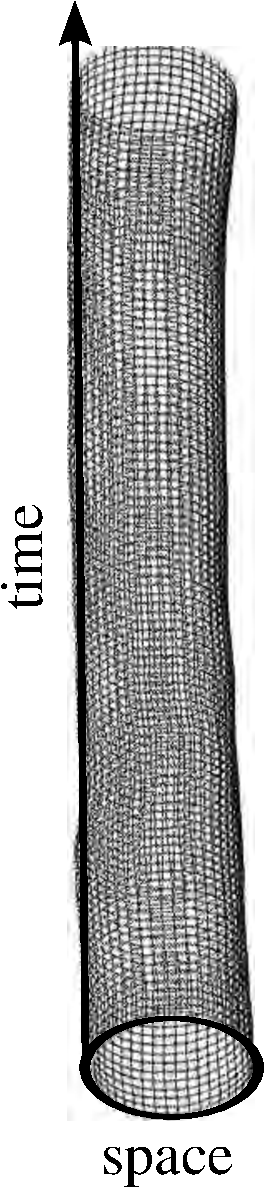
\includegraphics[width=.75\textwidth]{cylinderTime1}
    \vfill
\small{\texttt{(a)}}
\end{minipage}
~~~~
\begin{minipage}[height=.20\textheight]{.75\textwidth}
\centering
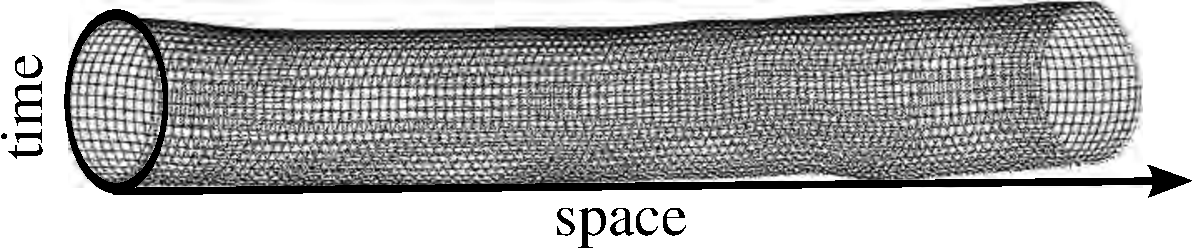
\includegraphics[width=.80\textwidth]{cylinderSpace1}
\\
\small{\texttt{(b)}}
\\
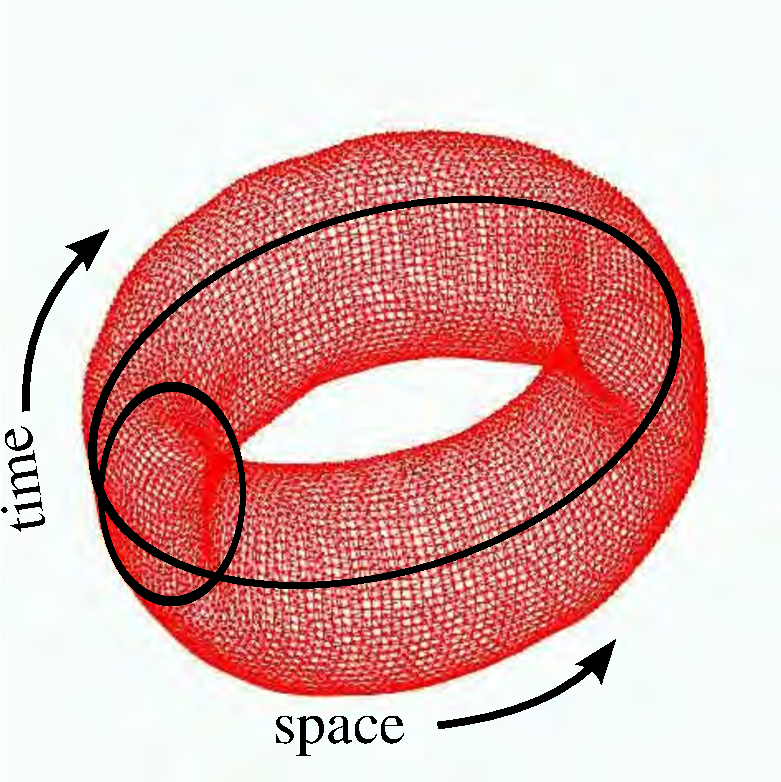
\includegraphics[width=.50\textwidth]{spaceTime1}
\\
\small{\texttt{(c)}}
\end{minipage}
    \end{center}
\caption{\label{fig:spaceTime1}
(a) The 1D \KSe\ is usually integrated on a \spt\ cylinder of an
    arbitrary fixed $\speriod{}$ periodic spatial extent, with time
    $\zeit\in\{-\infty,\infty)$; for an example, see \reffig{f:ks_largeL}.
(b) It is also possible to integrate the equation on a \spt\ cylinder of an
    arbitrary fixed $\period{}$ periodic temporal extent, with position
    ranging over $\conf\in\{-\infty,\infty)$, see \refsect{sect:KSspaceInt}.
(c) Here we shall seek {\spt}ly \twot\ solutions $u(\conf,\zeit)$ over a 2-torus of
    dynamically determined size $(\speriod{},\period{})$ , see
    \refsect{sect:KStwots}.
}
\end{figure}
%%%%%%%%%%%%%%%%%%%%%%%%%%%%%%%%%%%%%%%%%%%%%%%%%%%%%%


Smooth, spatially periodic velocity field $u$ %(\conf,\zeit)=u(x+\speriod{},\zeit)$
is naturally represented in the Fourier space,
\beq
  u(\conf,\zeit)
   =\sum_{m=-\infty}^{+\infty} a_m(\zeit)\,e^{ i 2\pi m\conf /\speriod{} }
\,,
\ee{eq:ksexp}
with the $1$D PDE \refeq{e-ksL}
replaced by an infinite set of
ODEs for the complex Fourier coefficients $a_m(t)$:
\beq
\dot{a}_m %= \pVeloc_m(a)
     = ( q_m^2 - q_m^4 )\, a_m
    - i \frac{q_m}{2} \sum_{k=-\infty}^{+\infty} a_k a_{m-k}
\ee{SCD07:expan}
where $q_m =  2\pi m/\speriod{}$.
Since $u(\conf,\zeit)$ is real, $a_m=a_{-mm}^\ast$, and we can replace the
sum by a $m > 0$ sum.


Consider the \KSe\ \refeq{e-ks} on a {\spt} cylinder
$(\conf,\zeit)\in([0,\speriod{}),\reals)$, defined on a a spatial strip of width
$\speriod{}$, with spatially periodic boundary condition $u(\conf,\zeit)=u(x+\speriod{},t)$, see
\reffig{fig:spaceTime1}\,(a).
Discretize spatially the \KS\ system by Fourier expanding the field
$u(\conf_n,\zeit)= u_n(\zeit)$ over $N$ points of a periodic spatial 1D
lattice $\conf_n=n\speriod{}/N$,
\bea
  \Fu_k(\zeit) &=& \frac{1}{N} \sum^{N-1}_0 u_n(\zeit) e^{-iq_k\conf_n}
  \,=\, \frac{1}{N} \sum^{N-1}_0 u_n(\zeit) e^{-i 2 \pi k n /N}
  \,,\quad
q_k = \frac{2 \pi k}{\speriod{}}
\continue
  u_n(\zeit) &=&\sum_{k=0}^{N-1}\Fu_k(\zeit) e^{iq_k\conf_n}
    \,=\, \sum_{k=0}^{N-1}\Fu_k(\zeit) e^{i 2 \pi k n /N}
\,,
\label{spatFT}
\eea
and expressing \refeq{e-ks} in terms of discrete spatial Fourier modes as
$N$ ordinary differential equations (ODEs) in time
\beq
%\dot{\Fu}_k(\zeit)
\frac{d~}{d\zeit}\Fu_k(\zeit)
= ( q_k^2 - q_k^4 )\, \Fu_k(\zeit)
- \frac{i q_k}{2} \!\sum_{k'=0}^{N-1} \!\!\Fu_{k'}(\zeit) \Fu_{k-k'}(\zeit)
\,.
\label{e-Fks}
\eeq

        \PCedit{
In the Fourier representation the \reqva\ time dependence is
\beq
 a_k(t) e^{-itc q_k} = a_k(0)
\,.
\ee{reqvaF}
Differentiating with respect to time, we obtain
the Fourier space version of the \reqv\ condition
\refeq{KSeqvCond},
\beq
 \pVeloc_k(a) - i q_k c a_k = 0
\,,
\ee{reqvCondF}
which we solve for (time independent) $a_k$ and $c$.
        }


%%%%%%%%%%%%%%%%%%%%%%%%%%%%%%%%%%%%%%%%%%%%%%%%%%%%%%%%%%%%%%%%%%
\subsubsection{Temporal stability}
\label{exam:KurSivTempstab}
% From ChaosBook Chapter{PDEs}{2016-01-23}{Turbulence?}

To calculate the temporal stability of a spatial \eqv\ $\Fu_\stagn$
    \PC{2019-05-16}{dropped
(or a temporally \po).
%\refeq{eq:StabMat} is plain wrong, no?
    }
we need to evaluate  the \stabmat\ (the matrix of temporal
velocity gradients)
\beq
%  \Mvar_{ij}(a_q)  = \left.\frac{\partial v_i}{\partial a_j}\right|_{a=a_q}
  \Mvar_{ij}(\Fu_\stagn)  =
  \left.\frac{\partial \dot{\Fu}_i}{\partial \Fu_j}\right|_{\Fu={\Fu_\stagn}}
\,.
\label{eq:StabMat}
\eeq
For \KS\ we can
compute $\Mvar(\Fu_q)$ efficiently using the linearity
of the Fourier transform, see \refref{SCD07}.
Consider the four matrices
$\frac{\partial \dot{b}_k}{\partial b_j},\frac{\partial
\dot{b}_k}{\partial c_j},\frac{\partial \dot{c}_k}{\partial
b_j},\frac{\partial \dot{c}_k}{\partial c_j}$,
where the real and imaginary parts of $\Fu_k$ are
$\Fu_k=b_k+ic_k$.
For illustration, consider the $b_k=0$ invariant antisymmetric subspace
$\bbU^+$,
\beq
\dot{c}_k= \pVeloc_k(c)
     = ( q_k^2 - q_k^4 )\, a_k
    - \frac{q_k}{2} \sum_{m=-\infty}^{\infty} c_m c_{k-m}
\,,\qquad   q_k = k/2\pi \speriod{}
\,.
\ee{expan}
The temporal {\stabmat} \refeq{eq:StabMat} restricted to the invariant
antisymmetric subspace $\bbU^+$ follows from \refeq{expan}:
\beq
{\Mvar}_{kj}(c) =\frac{\pde v_k(a)}{\pde c_j  }
=(q_k^2- q_k^4)\delta_{kj} + q_k ( c_{k-j}- c_{k+j})
\,.
\ee{expanMvar}
For the full \statesp, consult sect.~6.2 {\em Calculating stability of equilibria}
of Siminos thesis\rf{SiminosThesis}.

\subsubsection{\KS\ $u=0$ temporal equilibrium}
\label{sect:KSu0equiT}

The \KS\ flat flame front $u(\conf,\zeit)=0$ is always a temporal {\eqv} of \refeq{e-ks},
whose temporal {\stabmat} \refeq{expan} is
diagonal, with real temporal stability exponents $\eigExp[k]= q_k^2- q_k^4$,
the eigenvectors are spatial Fourier modes, and consequently the
temporal {\jacobianM} is diagonal as well,
\(
\jMps^t_{kj} = \delta_{kj} \ExpaEig_k(\zeit)
    \,,\;
\ExpaEig_k(\zeit) = e^{(q_k^2- q_k^4)\,t}
\,.
\)
%	} %end \example{\Stabmat,  antisymme
%%%%%%%%%%%%%%%%%%%%%%%%%%%%%%%%%%%%%%%%%%%%%%%%%%%%%%%%%%%%%%%%%%

% siminos/gudorf/thesis/chapter/KSspaceInt.tex
% $Author: predrag $ $Date: 2020-05-25 15:18:45 -0400 (Mon, 25 May 2020) $

%\subsection{Temporally periodic \KS}
%\label{sect:KSspaceInt}
%\hfill     2016-02-04 Burak

\MNGedit{

BLOG EXCERPTS

I would not use much time on improving integrators at this stage (the
flow is not Hamiltonian, but there is lots of literature on time-reversal
invariant dynamical systems - \refref{lamb98,LaWu02,Bosetti2010})

\begin{figure}[ht]
\begin{minipage}[height=.45\textheight]{.45\textwidth}
\centering \small{\texttt{(a)}}
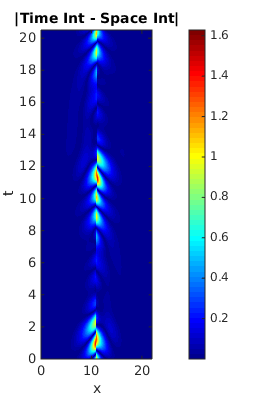
\includegraphics[width=\textwidth,height=.45\textheight]{MNGppo1m21e}
\end{minipage}
\begin{minipage}[height=.45\textheight]{.45\textwidth}
\centering \small{\texttt{(b)}}
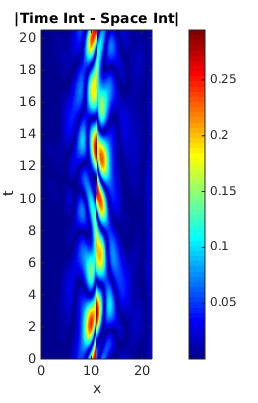
\includegraphics[width=\textwidth,height=.45\textheight]{MNGppo1m7e}
\end{minipage}
\caption{\label{fig:MNGppo1error}
Absolute error between time-integrated solutions of $\PPO{10.2}$ and spatially integrated solutions. A Time-periodic initial condition $T = [0,2\,T_{\PPO{10.2}})$ was taken from the time integrated solution. This initial time-strip was integrated spatially in two parts, $\conf = [0,11]$ and $\conf = [-11,0]$. The number of active Fourier modes in each plot are (a) 21, and (b) 7.
}
\end{figure}
}
Consider next the case of temporally periodic velocity field
\beq
    u(\conf, \zeit) = u(\conf, \zeit + \period{})
\label{e-PeriodicBC}
\eeq
on temporal domain of fixed period $\period{}$,
and any \conf, \ie, cylinder $(\conf,t) \in \reals \times [0,\period{})$, see
\reffig{fig:spaceTime1}\,(b).
%\KSe\ in one space dimension is
%\beq
%    u_\zeit =  - u u_\conf
%    -u_{\conf \conf}-u_{\conf \conf \conf \conf}\,,
%    \label{e-ks2}
%\eeq
%where subscripts denote partial derivatives.
In order to express
\KS\ as a set of first-order PDEs, define four fields
\beq
(u_{0},u_{1},u_{2},u_{3}) \equiv
(u,
u_{\conf},
u_{\conf \conf},
u_{\conf \conf \conf})
%    u_{0} \equiv u(\conf,\zeit) \,, \quad               % u^{(0)}
%    u_{1} \equiv u_{\conf}(\conf,\zeit) \,, \quad        % u^{(1)}
%    u_{2} \equiv u_{\conf \conf}(\conf,\zeit) \,, \quad  % u^{(2)}
%    u_{3} \equiv u_{\conf \conf \conf}(\conf,\zeit)      %  u^{(3)}
\,.
\eeq
Using the values of the four fields
%$(u_{0},u_{1},u_{2},u_{3})$
%$u( \conf_0, \zeit)$,
%$u_{\conf}( \conf_0, \zeit)$,
%$u_{\conf \conf}( \conf_0, \zeit)$,
%$u_{\conf \conf \conf}( \conf_0, \zeit)$,
for all $\zeit \in [0, \period{})$ at a fixed space point $\conf_0$,
as initial values,
one may attempt
to determine $u(\zeit, \conf)$ for any $\conf$ on a time-periodic strip
$\zeit \in [0, \period{})$ by solving the \KS\ \refeq{e-ks}
rewritten as a set of equations first order in spatial
derivatives
    \PC{2016-07-23}{The equations seem correct to me.
    The notation of \refrefs{LanThesis,lanCvit07} is different, but
    Burak's $u^{(j)}$ fields are easier to keep track of.
    {\bf 2019-05-18 PC} experimenting with $u_j$ format.
    }
\bea
    \frac{\partial}{\partial \conf} u_{0} &=& u_{1} \,,\quad
    \frac{\partial}{\partial \conf} u_{1} \,=\, u_{2} \,,\quad
    \frac{\partial}{\partial \conf} u_{2} \,=\, u_{3} \,, \label{e-ksX} \\
    \frac{\partial}{\partial \conf} u_{3} &=&
    - \frac{\partial}{\partial \zeit} u_{0} - u_{2} - u_{0} u_{1}
\nonumber
\,.
\eea
Given the time-periodic boundary condition \refeq{e-PeriodicBC},
it is natural to expand the \KS\ field $u(\conf,\zeit_n)= u_n(\conf)$ as a temporal Fourier
$u(\conf,\zeit_n)= u_n(\conf)$ over $M$ points of a periodic
temporal lattice $\zeit_n = n \period{}/M$, $n=0,1,\cdots,M-1$:
\beq
    u_{i}(\conf, \zeit) = \sum_{n = 0}^{M-1}
    \Fu_{i,n}(\conf)\,e^{i \omega_n \zeit_n} \, , \quad \mbox{where }
    \omega_n = 2 \pi n / \period{} \, .
\ee{BBtemporFourier}
Rewriting \refeq{e-ksX} in terms of temporal Fourier modes,
we obtain $4M$ ordinary differential equations,
\bea
\frac{\partial}{\partial \conf} \Fu_{0,n} &=& \Fu_{1,n}
         \continue
\frac{\partial}{\partial \conf} \Fu_{1,n} &=& \Fu_{2,n}
        \continue
\frac{\partial}{\partial \conf} \Fu_{2,n} &=& \Fu_{3,n}
        \label{e-FksX} \\
\frac{\partial}{\partial \conf} \Fu_{3,n}
      &=&
 - i \omega_n \Fu_{0,n} - \Fu_{2,n}
 - \sum_{n' = 0}^{M-1} \Fu_{0,n - n'} \Fu_{1,n'}
\,. \nonumber
\eea
%Due to their instabilities, these equations might
%be hard to integrate numerically.
    \PC{2016-09-12, 2016-09-23}{Checked, except for the range of $n'$.}

\subsubsection{Integrating \KS\ on a $\period{}=0$ line}
\label{sect:KSeqva}

    \PCedit{
[{\bf 2016-02-06 Predrag}
summarize the Michelson\rf{Mks86} case on the spatial $\speriod{}\to\pm\infty$ domain.
Review the reflection-invariant subspace discussed in
Lan's thesis\rf{LanThesis} and his thesis-work article\rf{lanCvit07,DoLa14}.
Then set up the full \On{2} equivariant case, and describe the
\On{2}-symmetry reduced case, following \refrefs{BudCvi14,BudCvi15}.
]
    }

%%%%%%%%%%%%%%%%%%%%%%%%%%%%%%%%%%%%%%%%%%%%%%%%%%%%%%%%%%%%%%%%
\begin{figure}[t]
\begin{center}
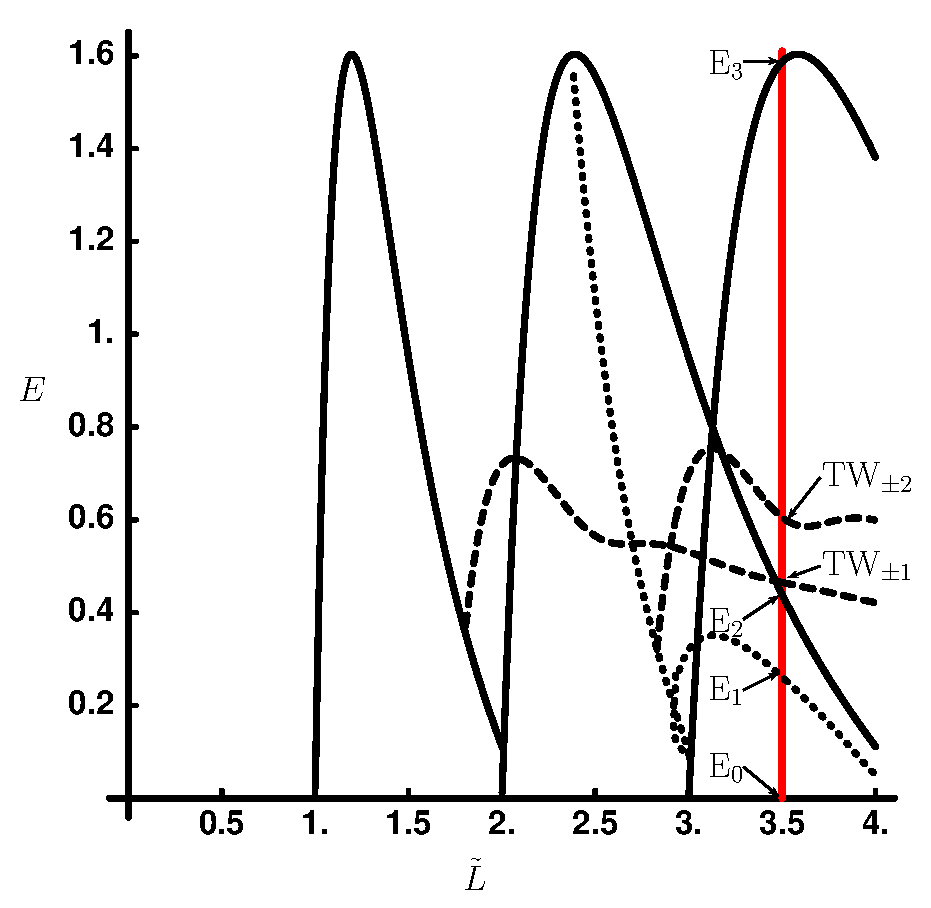
\includegraphics[width=0.5\textwidth]{ksBifDiag_pst}
\end{center}
\caption{\label{fig:SCD07ksBifDiag}
The energy \refeq{SCD07eq:stdks} %{ksEnergy}
of the \eqva\ and \reqva\ that
exist up to $\speriod{}=22$, $\tildeL = 3.5014\ldots$, plotted as a function
of the system size $\tildeL = \speriod{}/2\pi$ (additional \eqva, not present
at $\speriod{} = 22$ are given by Greene and Kim\rf{ksgreene88}). Solid curves denote
$n$-cell solutions \EQV{2} and \EQV{3}, dotted curves the GLMRT
\eqv\ \EQV{1},
and dashed curves the \reqva\ \REQV{\pm}{1} and \REQV{\pm}{2}.
The parameter $\alpha$ of \refrefs{KNSks90,ksgreene88} is
related to the system size by $\tildeL=\sqrt{\alpha/4}$.
(From Cvitanovi{\'c}, Davidchack and Siminos\rf{SCD07})
        }
\end{figure}
%%%%%%%%%%%%%%%%%%%%%%%%%%%%%%%%%%%%%%%%%%%%%%%%%%%%%%%%%%%%%%%%%%

%     BB 2016-02-04, PC 2016-09-23
If $u$ is a temporal \eqv, $u = u(\conf+v\zeit,0)$ whose spatial profile
does not change in time, with a vanishing $u_t=0$ (for an \eqv) or a constant
traveling wave velocity $u_t=v$ (for a \reqv), one can integrate \refeq{e-ks}
\beq
    u_\zeit -v = 0
    = - \left(u^2/2 -u_{\conf}-u_{\conf \conf \conf}\right)_{\conf}
\label{e-ksSteady}
\eeq
once over space, and the highest order derivative in \refeq{e-ksX}
becomes the third order\rf{Mks86,LanThesis,lanCvit07,DoLa14}. We shall
refer to this case as the $\period{}=0$ temporal strip, as specifying $u
= u(\conf_0,0)$ at $\zeit=0$ instant suffices to initialize the spatial
evolution, which in this case is given by a set of three ODEs and an
integration constant, which can be interpreted as the energy density $\expctE$,
\beq
\expctE = {\textstyle\frac{1}{2}}u^2 - c u + u_x + u_{xxx}
\,.
\label{SCD07eq:stdks}
\eeq
% \PCpost{2018-05-30}{
Computationally, it is more robust to compute $\expctE$ by averaging over $\speriod{}$,
as in \refeq{SCD07ksEnergy}.

Eqs.~\refeq{e-ksX}, however, remain a set of four PDEs for any
$\period{}>0$ temporal strip.

\subsubsection{Spatial stability of $u=0$ equilibrium}
\label{sect:KSu0equiS}

To calculate the spatial stability of a spatial \eqv, we need to evaluate
the \stabmat\ of the system in the complex representation \refeq{e-FksX}
in terms of the 16 sub-blocks
\beq
  \Mvar_{ij}^{IJ} (\Fu)  =
\frac{\partial \Fu^{'}{}^{(I)}_i}
     {\partial \Fu{}^{(J)}_j}
\,,\qquad
    \Fu^{'} = \Fu_x
\,.
\ee{eq:StabMatBlocks}
The trivial \eqv\ of \refeq{e-FksX} is given by $\Fu^{(I)}_{j}=0$.
In terms of $[M\!\times\!M]$ temporal Fourier modes blocks its spatial
\stabmat\ is
\beq
\Mvar^{IJ}(0) =
\begin{bmatrix}
  0 & 1 & 0 & 0 \\
  0 & 0 & 1 & 0 \\
  0 & 0 & 0 & 1 \\
\mbox{Diag}\{-i \omega_k\} & 0 & -1 & 0
\end{bmatrix}
\ee{PCeqvaStblty}
%Here
%\beq
%\begin{bmatrix}
%  0 & 1 & 0 & 0 \\
%  0 & 0 & 1 & 0 \\
%  0 & 0 & 0 & 1 \\
%Diag\{-i \omega_k\} & 0 & 0 & 0
%\end{bmatrix}
%\ee{PCcyclic}
%is cyclic of order 4 and thus has a nice characteristic equation, but the
%$\Mvar^{02} (\Fu) =-1$ screws that up.

% siminos/gudorf/thesis/chapter/KStwots.tex
% $Author: predrag $ $Date: 2020-05-25 15:18:45 -0400 (Mon, 25 May 2020) $

% called by
%           siminos/spatiotemp/chapter/spatiotemp.tex
%           siminos/tiles/GuBuCv17.tex

%\section{\KS\ on a torus}
%\label{sect:KStwots} % KSspacetime}

Here we propose to describe all solutions $u(\conf,\zeit)$ of \KSe\ \refeq{e-ks} as the
closure of the union of the set of all prime (non-repeating)
\twots\
\bea
u(\conf,\zeit) &=& u(\conf,t+\period{})
       \;=\; u(\conf+\speriod{},t)
\continue
       &=&  u(\conf+\speriod{},t+\period{})
\,,\quad
(\conf,\zeit)\in([0,\speriod{}),[0,\period{}))
\,.
    \label{e-ksTorus}
\eea

Consider a torus $(\speriod{},\period{})$ with {\spt}ly
doubly-periodic $u(\conf,\zeit)=u(x+\speriod{},t+\period{})$,
$(\conf,\zeit)\in([0,\speriod{}),[0,\period{}))$, see
\reffig{fig:spaceTime1}\,(c), and combine the discrete spatial
Fourier modes expansion \refeq{spatFT} with the discrete temporal Fourier
modes expansion \refeq{BBtemporFourier}.
Discretize $u(\conf_n,\zeit_m)= u_{nm}$ over
$N$ points of a periodic spatial lattice $\conf_n = n \speriod{}/N$,
and
$M$ points of a periodic temporal lattice $\zeit_m = m \period{}/M$,
%\beq
%    \Fu_{k,m}^{(i)} = \frac{1}{M} \sum_{n = 0}^{M-1}
%    \Fu^{(i)}_{k,n} e^{i \omega_n \zeit_m}
%    \, , \quad
%    \Fu^{(i)}_{k,n} = \sum_{m=0}^{M-1}\Fu_{k,m}^{(i)}  e^{-i \omega_n \zeit_m}
%    \, , \quad
%    \mbox{where }
%    \omega_n = 2 \pi n / \period{} \, .
%\eeq
%
\bea
\Fu_{kj} &=&
  \frac{1}{NM} \sum^{N-1}_{n=0} \sum^{M-1}_{m=0}
  u_{mn} \, e^{-i(\wavek \xm + \freqj \tn)}
    \,,\quad
\wavek = \frac{2 \pi k}{\speriod{}}
    \,,\;
\freqj = \frac{2 \pi j}{\period{}}
    \continue
u_{mn} &=&\sum_{k=0}^{M-1}\sum^{N-1}_{j=0}
   \Fu_{kj} \, e^{i(\wavek \xm + \freqj \tn)}
\,,
\label{spattempFT}
\eea
In its Fourier discretization, \KS\ PDE \refeq{e-Fks} is a set of $MN$
algebraic equations for the {\spt} Fourier coefficients $\Fu$,
\beq
\left[ i \freqj - ( \wavek^2 - \wavek^4 ) \right]\Fu_{kj}
+ i \frac{\wavek}{2} \!\sum_{k'=0}^{M-1} \sum^{M-1}_{j'=0}\!\!
\Fu_{k'j'} \Fu_{k-k',j-j'}
    = 0
\,.
\label{e-FksSpattemp}
\eeq
In other words, we have reduced the problem of either temporal or
spatial evolution on a
{\spt}ly periodic domain to the fixed point problem of determining an
invariant 2-torus, a fixed point in the $NM$\dmn\ \statesp.

\MNG{2019-05-13}{Elimination of space and time
translations effectively reduces the codimension of each solution by two, this is
undesirable when numerically solving the \refeq{e-pseudospectral} in a least-squares sense}
First, however, we must eliminate the temporal translation marginal eigenmode
by a {\PoincSec}, and the spatial translation marginal eigenmode by a {\slice}.
Generically, they both can fixed by the first Fourier mode {\PoincSec} /
{\slice}.
The Newton method then requires inversion of $1-J$, \ie,
$\det(1-J)$, where $J$ is the 2-torus \jacobianM.
    %
    \PC{2018-04-08}{see also \refsect{sect:KurSivSpTmpStab}.}

We can generalize the notion of average `energy' density
\refeq{SCD07ksEnergy} and apply it to any \twot\ $p$ by also
averaging over time
\beq
    \expctE_p=
  \frac{1}{\speriod{}\period{}}\!\oint d\pSpace\oint d\zeit \frac{u^2}{2}
  \,,
  \label{twotEnergy}
\eeq
The Fourier space average spatial energy density \refeq{SCD07EFourier}
generalized to any {\spt} solution \refeq{spattempFT} is then:
\beq
\expctE
          =  \sum_{k=0}^{N-1}\sum^{M-1}_{n=0}
             {\textstyle\frac{1}{2}}|\Fu_{kn}|^2
\,.
\ee{twotEFourier}


\subsection{Spatiotemporal $u=0$ equilibrium}
\label{sect:KSu0equiST}

    \PC{2019-03-16}{
    Incorporate here the spatial evolution stability analysis of
    blog posts starting with {\bf 2016-09-02 Matt Stability of u=0 equilibria}.
   }
   %
Consider the $\Fu_{kn}=0$ \eqv\ of \refeq{e-FksSpattemp}. Its
linearization is
    \MNG{2016-09-12 }{
\MNGedit{Added the factor of $i$ that was missing in \refeq{e-FksSpattemp}}
\PCedit{2016-09-23 restored signs to match \refeq{e-Fks} and \refeq{e-FksSpattemp}}
    }
\bea
i \omega_n  &=&  q_k^2 - q_k^4
    \continue
i \frac{2\pi n}{\period{}}   &=&
\left(\frac{2\pi k}{\speriod{}}\right)^2 - \left(\frac{2\pi k}{\speriod{}}\right)^4
\,.
\label{e-FksSpattemp0}
\eea
The two special cases are the spatial strip of \refsect{sect:KStimeInt},
which yields the $2N$ real temporal stability exponents
$\Lyap_k=i\omega(k)$ for a fixed spatial strip of width $\speriod{}$, and the
temporal strip of \refsect{sect:KSspaceInt}, which yields the $4+8(M-1)$ complex
spatial stability exponents $i q^{\pm,\pm}(n)$ for a fixed temporal strip of period
$\period{}$, as the four solutions of the quartic equation \refeq{e-FksSpattemp}
for each $i \omega_n$, $n = 0, \pm 1, \pm 2, \pm M/2$ :
\beq
(i q_k)^4 + (i q_k)^2 + i \omega_n  =0
    \quad\Rightarrow\quad
i q^{\pm,\pm}(n) = \pm \sqrt{(-1\pm \sqrt{1 -4 i \omega_n})/2}
\ee{spatialStabExp}
    \MNG{2016-09-20}{
    I think I should have been looking for $i q_k$ not $q_k$? If so, it
    matches the stability exponents of \refeq{PCeqvaStblty} %\refeq{MNGeqvaStblty}
    }
Each solution appears twice, corresponding to  $(\omega_n,-\omega_n)$,
except for
\beq
q^{\pm,\pm}(0) = \mp i\sqrt{(-1\pm 1)/2} =
(0,0,-1,1)
\,.
\ee{spatialStabExp0}
There are two root magnitudes for each $n \neq 0$, independent of the
sign of $n$:
%\[%beq
%|q^{\pm,\pm}(n)|^2 = (-1\pm \sqrt{1 +4 i \omega_n})
%(-1\pm \sqrt{1 -4 i \omega_n})/4
%\]%ee{spatialStabExp01}
%
\beq
|2q^{\pm,\pm}(n)|^2 = 1+ \sqrt{1 +  16 \omega_n^2}
\pm \sqrt{1 +4 i \omega_n}
\pm \sqrt{1 -4 i \omega_n}
\,.
\ee{spatialStabExp1}

\subsection{Spatiotemporal stability}
\label{sect:KurSivSpTmpStab}

Let
$u_\stagn(\conf,\zeit)$ be a doubly-periodic solution of \refeq{e-FksSpattemp} on the
$(\conf,\zeit)\in[0,\speriod{})\times[0,\period{})$ torus, a point in the
$\speriod{}\,\period{}$\dmn\ \statesp. Add an arbitrary small perturbation field
$\delta u(\conf,\zeit)$, also doubly periodic. Linearize \refeq{e-FksSpattemp}.
The linearized operator acting on $\delta u(\conf,\zeit)$ must annihilate it, \ie,
(WRONG AS IT STANDS)
\[
(J(u_\stagn) -\ExpaEig_j \matId)\delta u =0
\]
where the \jacobianM\ is the linearization over the whole 2-torus
\beq
J(\Fu_\stagn)_{kn} =
\left[ i \omega_n - ( q_k^2 - q_k^4 ) \right]\delta_{kn}
+ i q_k\!\sum_{k'=0}^{N-1} \sum^{M-1}_{m'=0}\!\!
\Fu_{k'm'} \delta_{k-k',m-m'}
\,.
\label{e-FksSpTmpJac}
\eeq
In $d=1$ case (pure temporal evolution) $\det(J(u_\stagn) -\matId)$ is the
usual period $\period{}$ cycle weight, this time obtained not by integration in
time but by evaluating the determinant of the Toeplitz matrix over the whole
cycle in one go (this might be familiar to some from the path-integral
derivation of Gutzwiller formula cycle weight. With \refeq{e-FksSpTmpJac},
$\det(J(u_\stagn) -\matId)$ is the pattern weight in $d=2$, and this
generates to defining the invariant weight for any $d$-torus.
 
%\begin{description}
\item[2017-01-23 Predrag]
not sure where to put this - into pipe blog or here, but
Wang \etal\rf{WGBGQ13}
{\em Towards scalable parallel-in-time turbulent flow simulations}
introduces ``the least squares shadowing (LSS) method'' and
uses \KS\ to illustrate the power of their method: ``
The initial condition is relaxed and information is allowed to propagate
both forward and backward in time. [...]
next-generation simulation paradigm can likely be spacetime parallel
simulations. These simulations subdivide the four-dimensional spacetime
computational domain. Each computing core handles a contiguous subdomain
of the simulation spacetime. Compared to subdivision only in the
three-dimensional space, spacetime parallel simulations can achieve
significantly higher level of concurrency, and reduce the ratio of
inter-core communication to floating point operations. [...]
Efficient time domain parallelism can only be achieved through
reformulating turbulent flow simulation into a well-conditioned problem.
We reformulate turbulent flow simulation into a well-conditioned problem
by relaxing the initial condition.
 [...]
Instead of trying to find the flow solution that satisfies both the
governing equation and the initial condition, we aim to find a flow
solution satisfying only the governing equation.
 [...]
Stability of the trajectory with a relaxed initial condition is achieved
by splitting a perturbation into stable and unstable components, and
propagating their effects forward and backward in time, respectively.
''

Blonigan and Wang\rf{BloWan14,BloWan15,BloWan16} might also be of interest.
ond one might not be as serious
in next generation HPC platforms.

\PCpost{2017-03-09}{
Andrej Junginger, J\"org Main, G\"unter Wunner and Rigoberto Hernandez,
{\em Variational principle for the determination of unstable periodic orbits
  and instanton trajectories at saddle points},
\arXiv{1703.02472}
(Prof. Uzer knows the authors well) write: ``
  The complexity of arbitrary dynamical systems and chemical reactions, in
particular, can often be resolved if only the appropriate periodic orbit - in
the form of a limit cycle, dividing surface, instanton trajectories or some
other related structure - can be uncovered. Determining such a periodic orbit,
no matter how beguilingly simple it appears, is often very challenging. We
present a method for the direct construction of unstable periodic orbits and
instanton trajectories at saddle points by means of Lagrangian descriptors.
Such structures result from the minimization of a scalar-valued phase space
function without need for any additional constraints or knowledge. We
illustrate the approach for two-degree of freedom systems at a rank-1 saddle
point of the underlying potential energy surface by constructing both periodic
orbits at energies above the saddle point as well as instanton trajectories
below the saddle point energy.
}

\NBBpost{2014-11-15,2017-01-26}{
Fazendeiro, Boghosian, Coveney and L{\"a}tt\rf{FBCL10}
{\em Unstable periodic orbits in weak turbulence}
seem to have applied the variational periodic orbit finding method to fluid
flow by parallelizing the whole thing.
    }

\PCpost{2017-05-05}{
Boghosian \etal\rf{BFLTC11} {\em New variational principles for locating
periodic orbits of differential equations} is
the most detailed discussion (see also \refrefs{BBLTFC11,FBCL10}):

They reformulate the space–time algorithm of Lan and
Cvitanovi\'c\rf{lanVar1} in a clear-headed way, and use
using the methods of gradient descent or conjugate
gradients to solve the variational equations.

They apply it to the lattice-Boltzmann method for the solution of the
Navier–Stokes equations, with a fully parallel implementation using the
Message Passing Interface.
The method has first been tested on the Lorenz equations\rf{BBLTFC11}.
They apply this to weak homogeneous turbulence driven by an
Arnold–Beltrami–Childress force field in three spatial dimensions. Because
the algorithm requires storage of the space–time lattice, even the smallest
orbits require resources on the order of tens of thousands of computing
cores. Using this approach, two UPOs have been identified and some of their
properties have been analysed.

In \refref{FiBoKo05} they discuss ``Ginzburg–Landau-type minimization.''
(Probably not worth pursuing, they do not return to it)

''    }

The ``adjoint periodic shadowing methods'' papers are rather tedious read (lots of
variational equations!):

Cacuci\rf{Cacuci81} {\em Sensitivity theory for nonlinear systems. {I. Nonlinear}
functional analysis approach} is cited by many authors up to 2019, with suggestive
paper titles, like

Luchini and Bottaro\rf{LucBot14} {\em Adjoint equations in stability analysis}

Cacuci\rf{Cacuci15} {\em Second-order adjoint sensitivity analysis methodology
(2nd-{ASAM}) for computing exactly and efficiently first- and second-order
sensitivities in large-scale linear systems: {I. Computationa}l methodology}

Cacuci\rf{Cacuci19} {\em Second-order sensitivities of a general functional of
the forward and adjoint fluxes in a multiplying nuclear system with source}:
\\
2nd-order (Hessian) sensitivity information accelerates the
convergence of optimization algorithms.
\\
In atmospheric
sciences ``second-order adjoint
models" were used to compute products between the Hessian of the cost
functional and a vector (representing a perturbation in sensitivity analysis, a
search direction in optimization, an eigenvector, etc.) to perform sensitivity
analysis of the cost function with respect to distributed observations.


\PCpost{2017-11-03} {
\HREF{https://scholar.google.com/citations?hl=en&user=6pzhrnkAAAAJ}{Jianke
Yang}\rf{Yang15} {\em A numerical method for computing time-periodic solutions
in dissipative wave systems} is another paper that finds \KS\ and \cGL\ {\rpo}s
using spatiotemporal methods.

It looks quite interesting, but it will requires bit of work to understand the
paper. Yang's Matlab codes are available
\HREF{http://www.cems.uvm.edu/~jxyang/codes.htm} {online}, so one can download
his \KS\ code and give it a go on some of our solutions.
   
Wang\rf{Wang13}
{\em Forward and adjoint sensitivity computation of chaotic dynamical systems}
has 44 citations.
It uses Lyapunov eigenvector decomposition for sensitivity analysis, but
that has high computational cost when the dynamical system has many
positive Lyapunov exponents.

Blonigan and Wang\rf{BloWan13}
{\em Multigrid-in-time for sensitivity analysis of chaotic dynamical systems}:

Wang\rf{Wang14} {\em Convergence of the least squares shadowing method for
computing derivative of ergodic averages}

Their papers say that LSS was introduced in
Wang, Hu and Blonigan\rf{WaHuBl14} {\em {Least Squares Shadowing} sensitivity
analysis of chaotic limit cycle oscillations}. The paper has 42 citations.
%, many of which are self-citations.

LSS computational cost is $O(mn^3)$ where $m$ is the number of time steps, and
$n$ is the number of dynamical degrees of freedom.

When the dynamical system is high dimensional, e.g., a discretized
partial differential equation, iterative solution methods should be used
instead of direct matrix solvers. Because the system is well-conditioned
and only twice as large as an initial value problem, an iterative
solution can potentially cost only a small multiple of an initial value
solution.

What I do not get is
the cost function - it is usual squares, but with respect to a
``pre-specified reference trajectory.''

\emph{Sensitivity analysis}\rf{LeAlHa00} computes the derivative of outputs to inputs
(derivative with respect a control parameter) of a
simulation. Conventional methods, including the tangent and the adjoint method,
fail when the dynamical system is chaotic and the outputs are long time averaged
quantities.

ensemble adjoint method\rf{LeAlHa00}

\index{sensitivity!analysis}

Chater \etal\rf{CNBW17} {\em Least squares shadowing method for sensitivity
analysis of differential equations}

Chater, Ni and Wang\rf{ChNiWa17} {\em Simplified {Least Squares Shadowing}
sensitivity analysis for chaotic {ODEs} and {PDEs}}

Blonigan and Wang\rf{BloWan18} {\em Multiple shooting shadowing for sensitivity
analysis of chaotic dynamical systems} present a variation of the method suitable
for high-dimensional systems, using multiple-shooting strategies.

Craske\rf{Craske19}
{\em Adjoint sensitivity analysis of chaotic systems using cumulant truncation}

Blonigan\rf{Blonigan17} {\em Adjoint sensitivity analysis of chaotic dynamical
systems with non-intrusive least squares shadowing} introduces a ``non-intrusive
least-squares shadowing (NILSS)'' algorithm.

Ni and Wang\rf{NiWan17} {\em Sensitivity analysis on chaotic dynamical systems by
{Non-Intrusive Least Squares Shadowing ({NILSS})}}

Ni\rf{Ni19} {\em Hyperbolicity, shadowing directions and sensitivity analysis of
a turbulent three-dimensional flow} uses the NILSS algorithm.

Kim and H. Choi\rf{KimCho14}
{\em Space-time characteristics of a compliant wall in a turbulent channel flow}

\PCpost{2019-03-19} { {\bf to Matt}
One of our problems is that we do not know what our spatiotemporal
variational method is called by other people who have presumably already
crossed this bridge before us.

Most recently, Pepper has been working on how to
equip Las Vegas firemen with real time info which way the plumes are going, see
Pepper and Gonzalez\rf{PepGon18} {\em A localized meshless technique for
generating {3-D} wind fields}. For us Sect.~4. {\em The Meshless Method} is
helpful, as a succint summary. The point there is that they replace a
square mesh by support on a set of irregularly placed points (for
example, Las Vegas firehouses). Few bullet points from his talk

\begin{enumerate}
  \item
boundary element methods reduce the problem by one dimension (boundary
instead of the bulk)
  \item
Local Petrov-Galerkin good for steep gradients, \ie, shocks
  \item
Mashless methods work for Navier-Stokes, heat transfer, etc. They work
with primitive equations (velocity fields) rather than with vorticities,
as boundary conditions are difficult in the vorticity formulations.
  \item
Multiquadrics are good as they have explicit expressions for derivatives
  \item
Global mashless equation (linearized?) is a large matrix equation.
It can suffer poor conditioning, and is
efficient only for square domains.
  \item
Local mashless methods loop through all points one by one. They are
not ill conditioned.
  \item
They are engineers, they are happy if solutions are good to a few \%.
  \item
FreeFEM finite element code is free and can be downloaded
  \item
In atmospheric simulations: minimize variance between the observed and
the computed.
  \item
My feeling: meshless methods are good for inhomogenous discretizations, funky
boundary conditions. In our case, spectral methods (Fourier represenatations)
probably work better.
\end{enumerate}

The rest is my reading.
The meshless method was introduced by Fasshauer\rf{Fasshauer02} from whom
I gleaned this:

    They are interested in the numerical solution of a generic nonlinear
    (elliptic) PDE as a boundary value problem on some domain. Instead of
    discrete meshes, they work with the globally supported radial basis
    function (RBFs). Not clear to me how well these bases can be used on
    periodic domains. Globally supported multiquadric radial basis
    functions can be used for Newton iteration numerical solution of
    nonlinear partial differential equations. The use of coarse meshes
    during the initial iterations along with a multiquadric parameter
    which is adjusted with the meshsize increases the efficiency and
    stability of the algorithm.

    Fasshauer\rf{Fasshauer02} ``test problem'' is a nonlinear elliptic
    (\ie, a single $2D$ Laplacina) PDE on a unit square, different from
    but not totally irrelevent for our \KS\ application: he computes what
    we would call solution $u(t,x)$ over a quadratic domain, compatible
    with the given PDE. His solutions are of much simpler shape than most
    of Matt's solutions, so Matt seems to be solving a harder problem.

If of interest, try to check out the Fasshauer book\rf{Fasshauer07} with MATAB
codes.
Maybe we also have to learn about ``Nash iteration'' and the
Kansa\rf{KansaI90,KansaII90} or ``multiquadric method'' for solving problems in
2D and 3D arbitrary domains. Engineers like it for applying it to inhomogeneous
and irregular complex geometries. Closer to home, it has been used for computing
solutions to Burger's equation\rf{GaoChi14,SarAmi14}.

    }

\end{description}

\subsection{Adjoint sensitivity analysis}
\label{sect:AdjSenAn}

Sensitivity analysis, according to
\HREF{https://docs.juliadiffeq.org/latest/analysis/sensitivity.html}
{Julia}:

The local sensitivity of a solution of an ODE or a PDE model is given by the
derivative of the $i$th independent field of the solution with respect to the
$j$th parameter,
\( {\pde u_i}/{\pde p_j}. \)
There are three types of sensitivity analysis.
Local forward sensitivity analysis gives the gradient of the solution  along the
time evolution with respect to a parameter.
Local adjoint sensitivity analysis gives the gradient of some
functional of the solution, such as a cost function.
Global sensitivity analysis methods computes the
sensitivity over a domain without calculating derivatives.

Adjoint sensitivity analysis is used to find the gradient of the solution
$x(t,p)$ with respect to some functional of the solution. This adjoint requires
the definition of a scalar observable $a(x)$ where $x$ is a solution to the
differential equation.
Adjoint sensitivity analysis finds the gradient of
the integrated observable
\beq
A^t (x_0,p) = \int_{0}^{t}d\tau a(x(\tau,p)),
\ee{ASintObs}

I also like this
\HREF{https://marcschwalbach.com/posts/2016/5/29/a-taste-of-adjoint-sensitivity-analysis}
{introduction} by Marc Schwalbach. Unfortunately he lost steam after one post :)
For a weatherman's angle, see
Errico\rf{Errico97} {\em What is an adjoint model?}.


Traditional adjoint sensitivity methods face fundamental limitations when applied
on turbulence, which are addressed by development of robust methods for adjoint
analysis\rf{WaHuBl14}. %[15].

Over the past two decades it has been established that the
numerically exact invariant solutions of the Navier-Stokes
equations (``recurrent flows") serve as the ``building blocks" that
shape turbulent dynamics.

This dynamical framework  will be used to solve (and design) turbulent drag
reduction and optimisation problems in turbulence, in particular design of
compliant surfaces for drag reduction in plane channel flow.

Lasagna and Sharma are developing so called adjoint-based variational methods for
sensitivity analysis. With sensitivity information, they can design optimal
drag-reducing surfaces by using gradient-based optimisation methods.

The existing periodic orbit theory, so far successfully applied
only to low-dimensional dynamical systems, posits that the
description of the chaotic / turbulent state space is given by
ensembles of hierarchically organised unstable period solutions of
increasing length.
In contrast, Lasagna's working hypothesis is that a few periodic orbits of long
periods, embedded in state-space regions most frequented by turbulence and thus
capturing the full range of dynamical events, suffice. Which strategy works best
in practice remains an open question, and the approach proposed here should
certainly be explored.

They plan to develop new space-time parallel numerical methods to
find periodic orbits with long period and then develop adjoint
solverss
(formulated as a boundary value problem with periodic boundary condition)
to obtain gradient information.

The approach is based on the idea that adjoint analysis of such
structures can provide accurate sensitivities of time averaged
quantities with respect to the design surface parameters.


The proposed adjoint approach offers the ability to obtain
gradient information
with respect to a large number of parameters (the spatial
distribution of material properties)

For small perturbations, the sensitivity of a system is given by
the gradient with respect to a parameter.
Lasagna and Sharma have shown that this gradient can be obtained by
adopting adjoint techniques to periodic orbits.

A variation of any of the system's parameters (the viscosity in
case of {Kuramoto-Sivashinsky}) produces a computable state-space
distortion of periodic trajectories. They illustrate this by
varying viscosity $\nu$ from $(2\pi/39)^2$ to $(2\pi/38.5)^2$
for their shortest periodic orbit.

They compute a few thousand periodic orbits of period $\simeq 1000 \nu$. The
question is: what is the right orbit to use?

    \PC{2019-03-19} {It is Japanese heresy all over again (see comments at the
                     end of this section)}
They plan to consider only one periodic orbit, having a sufficiently long period
such as to span all possible dynamical events encountered by long chaotic
trajectories, i.e. shadowing many shorter, more elementary recurrent structures.
This is a different direction, where long-period orbits capture statistics of
turbulence.
The approach is based on empirical evidence
that, at least for low dimensional systems, the
variability across periodic orbits of similar
period $T$, e.g. the standard deviation of distribution
follows
the central limit theorem and decreases as
$1/\sqrt{T}$.

They view
turbulent flows as stationary equilibria of a four-dimensional PDE,
the Navier-Stokes equations in three spatial directions plus time,
with periodic conditions in time justified by the invariance under
time translation of statistically developed flows. With
sufficiently long temporal domains (akin to spatial domains larger
than a minimal flow unit), they expect that averages and their
gradients will converge with the size of the temporal domain.

Their goals are to a) demonstrate that these \po s
exists in Navier-Stokes problems b) develop an
understanding of their significance in describing turbulent
structure and evolution, b)
formalise a framework for control and optimisation of turbulence.

{\bf Time-parallel methods for long orbits}
They plan to develop new computational methods, suitable for arbitrarily long
orbits.

The system arising in the Newton search iterations is the
adjoint of this.
The
global-in-time nature of the adjoint problem on periodic orbits
enables mixed space/time domain decomposition methods, to
distribute computation across independent nodes of a
distributed memory system.

They use multiple-shooting techniques, exploiting time as an
additional direction for distributed memory parallelism. The
approach consists in partitioning the temporal interval into
independent sub-domains and than seeking the terminal adjoint
solution at the shooting points, imposing that the solution is
globally periodic and continuous at the shooting points.
    \PC{2019-03-19} {Just to drive Predrag more bewildered, they plot time
                     horizontally, space vertically :)}

Matrix-vector products for the construction of the Krylov basis
vectors in the GMRES solver can now exploit the block-banded
structure of this problem, by distributing the
sub-matrix/sub-vector products to different computational nodes in
a time-parallel fashion, and using independent adjoint
time-steppers to calculate actions, with minimal communication
required. Mixing spatial/temporal parallelism, via processor
grouping routines is a natural
extension.

Even if the proposed approach based is likely not applicable to
high-Reynolds number flows, the work holds the potential to accelerate
future development of adjoint methods suitable for chaotic systems\rf{LaShMe18}. % [16].


Task A.1 – This will be based on in-house codes under development at Southampton and
freely available software (e.g. J Gibson's channelflow). The influence of
the compliant wall will be modelled by linearised kinematic boundary
conditions, using standard modelling procedures\rf{LuShMc16,KimCho14}. % [12,7,11].


{\bf Space-time parallel algorithms for long periodic orbits.}

A dedicated c++ parallel Krylov
subspace library being developed at Southampton
\HREF{https://github.com/gasagna/ParK} {gitHub.com/gasagna/ParK}. The
Newton-Krylov-hookstep\rf{Visw07b} % [14]
approach will be used. They will
initially rely on temporal parallelism and subsequently extend the
library to spatial parallelism.

{\bf Space-time parallel adjoint solver.}
We will then couple
the adjoint time steppers developed in B.1 with the available
parallel Krylov solver to solve the adjoint boundary value problem.


The intersection of recurrent flow analysis with adjoint
techniques for optimisation is largely unexplored. So far,
recurrent flows have been primarily used as a proxy to understand
dynamics, i.e. as an analysis tool. Their program is
complementary to our efforts, because they aim to employ these
ideas for control and design.

\bigskip


From \texttt{siminos/blog/UPO.tex}:
\begin{description}
\item[2012-05-13  Predrag] [...] until the first unstable periodic solutions of
Navier-Stokes were computed by Kawahara and Kida\rf{KawKida01} in 2001,
determining such solutions seemed utterly out of reach. Their
`upper' periodic orbit appears embedded in the turbulent sea, and
captures statistics so well that it lead to the `Heresy', a belief of the
innocent that there exists a \emph{single} periodic orbit (!) that
captures turbulent statistics; we do not cite these papers, as
that was a vain hope of those too busy to read ChaosBook.org.

\item[2011-11-15  Predrag] From \texttt{pipes/blog/Alabama.tex}:
\\
Can you try this?
Compute the averages for $(D(t),I(t))$ for one period of
$\rpo{36.92}$ and for your $S$-subspace turbulent trajectory. That should
yield two point on the diagonal.  Kawahara was lucky there - they were
unreasonably close, the root of the Japanese Heresy. If they are not close,
$\rpo{36.92}$ does not go through the most concentrated regions of natural
measure.

From \refref{SCD07}: ``
Similarly close prediction of mean dissipation rate in the
 from a single-period \po\ computed by
Kawahara and Kida\rf{KawKida01} has lead to
optimistic hopes that `turbulence' is different from
low-dimensional chaos, insofar that the determination of one special
\po\ could yield all long-time averages.
Regrettably, not true -- as always, here too one needs a hierarchy
of \po s of increasing length to obtain accurate
predictions\rf{DasBuch}.
    ''


\item[2007-11-28 Predrag: Japanese heresy]
We do not want to refer to wrong papers, but here it is, for
the internal record, so we do not forget not to cite it:

Mitsuhiro Kawasaki and Shin-ichi Sasa\rf{KaSa05},
    ``Statistics of unstable periodic orbits of a chaotic dynamical system
    with a large number of degrees of freedom.''

\item[2012-08-12  Predrag]
Goldobin\rf{Goldobin12} \emph{Limit distribution of averages over
unstable periodic orbits forming chaotic attractor}, \arXiv{1208.1691},
is much weirder still: it is motivated by the Japanese Heresy and cites
only the Maryland non-theory paper as the source on the periodic orbit
theory.  Remind him to cite ChaosBook.

\end{description}


\section{Spatiotemporal literature - a blog}
\label{sect:SpatTempLit}

\begin{description}

\MNGpost{2018-07-17}{

\textbf{Notes on Literature review in thesis proposal}
I tried to motivate the need to go spatiotemporal by the wall that's been
hit in pipe and channelflow while still celebrating the amount of work
that codes like \texttt{channelflow} and \texttt{openpipeflow} have been
able to accomplish. It probably comes off as arrogant and I need to
rewrite it but I'm trying to get the point across that: There are lots of
people stepping back and trying to find other paths to solving the issues
of high-dimensional systems because the direct approach is providing
diminishing returns.

Don't mind all of the names and bibtex references, it was just
brainstorming that I didn't remove.
     }

\PCpost{2018-07-21}{``Lots of people stepping back and trying to find other
paths?'' Only our Wednesday Hangout crowd has computed Navier--Stokes
\ecs s\ in small computational domains, and I'm not aware of anyone
thinking of ``other paths'' to computing \ecs s\ in spatially infinite
domains other than you and me. Looking forward to reading the literature
review of these many paths that I'm unaware of.
}

\MNGpost{2016-09-06}{ {\bf ChronotopicApproach}
I've been reading \refrefs{LePoTo96, LePoTo97, PoToLe98,GiLePo95}
on Chronotopic theory of spatiotemporal chaos.

Branching out to get a better grasp of what's out there, I read a paper
Pikovsky and Politi\rf{PikPol98}, see %\refsect
{sect:PikPol98} in \texttt{blogCats}.
    \PC{2016-09-06}{Pikovsky and Politi\rf{PikPol98} is a stat mech paper about
    using KPZ equations in pattern formation, do not waste time on it right now}
It discusses the complex Ginzburg-Landau, two types of coupled maps, as
well as \KSe, so I thought it might be useful somehow.
}

\MNGpost{2017-10-31}{
Read the paper added to the bib file by Burak, {\em Towards a statistical
mechanics of spatiotemporal chaos} by Politi and Torcini\rf{PolTor92b}.

{\bf Predrag 2018-01-20} moved all Politi and Torcini\rf{PolTor92b} blogposts
to \texttt{blogCats}, dailyCats.tex.
}


    \PCpost{2016-11-10}{
Sobolev norms we have pondered a lot (sprinkled through various blogs) but for
now stick to the L2 (AKA Euclidean) norm.

Papers to read, possibly to test your variational
    code on the soultions reported there:

Rempel\etal\rf{RCMR04} {\em Analysis of chaotic saddles in high-dimensional
dynamical systems: the {Kuramoto-Sivashinsky} equation}.
Only in the antisymmetric subspace $\bbU^+$, periodic on $2\pi$ and vary
hyper-viscosity $\nu$. Might be good - do not know. For some reason neither
Siminos nor Budanur nor Xiong seem to have looked at this paper, nor the
subsequent ones.

Saiki\etal\rf{SYCMR15} {\em Reconstruction of chaotic saddles by
classification of unstable periodic orbits: {Kuramoto-Sivashinsky} equation}:
they work only in the antisymmetric subspace $\bbU^+$, see their Eq.~(3), but are
periodic on $2\pi$ and vary hyper-viscosity $\nu$, so you'll have to convert.
Looks like cut and paste of their earlier \refref{RCMR04}.
They use the PIM triple method\rf{pimyk,ReCi05}. BTW, calling a \po\  UPO is
like saying ``I am riding unstable bicycle'' every time you get on a bike
(all bicycles are unstable): `Note that our notation ``a-UPO'' may sound
awkward when expanded as ``attractor-unstable periodic orbit.''' In all
fairness, stupider things are known, like ``nonchaotic orbit" instead of \po,
check the next cubicle :)

What is obvious from looking at a paper like this one is that spacetime
invariant 2-tori persist in continuous families, as one change the domain
size $L$, so that must mean an additional marginal direction eigenvector for
the torus-finding variational routine...

Croft's papers\rf{CroDav06,Crofts07thesis,CroDav09,CrDaGo16} probably use
pseudoinverse - Levenberg-\-Marq\-uardt described in an appendix of
\refref{SCD07} is might be an example.
    }

\MNGpost{2016-12-20}{
Read through half of Moser\rf{moser86}. It is indeed hard to read but I'm
hoping that in conjunction with de la Llave's \textit{Introduction to KAM
Theory} I will get something out of it.

Read through about a quarter more of Trefethen\rf{Trefethen97} as well as went to
the physical library to skim some texts that another student recommended
for me. They were math texts on par with Moser\rf{moser86} about functional
analysis.
Read some more of numerical linear algebra, Trefethen\rf{Trefethen97},
starting to enjoy it as I think it is written quite well.

% While interesting, I decided to leave in the library for the
% rainiest of days.
    }


\MNGpost{2017-05-05}{Read Boghosian \etal\rf{BFLTC11}.
        }

\MNGpost{2017-05-08}{
I was reading a number
of papers\rf{Meza95,Chu09,BroWal97,MiAK03} having to do with
ill-conditioned linear systems and how to circumvent issues with GMRES.
}

\MNGpost{2017-06-06}{
Read some Guckenheimer\refref{guckb}
}

\MNGpost{2017-09-05}{Read Junginger \etal\rf{JuMWuHe17}
{\em ez, “Variational principle for the determination of unstable periodic
orbits and instanton trajectories at saddle points}, I think it could possibly
introduce some important topics.
}

\MNGpost{2017-04-14}{ I've been reading a bunch of papers\rf{TBAMR92} on
preconditioning methods; and specifically for GMRES algorithm.
}

\MNGpost{2018-01-23}{
Browsed through arXiv to try to survey the recent literature in fluid dynamics and chaotic dynamics fields
just to try and branch out a little bit so that my world view isn't a single leaf of the forest. Trying
not to spend too much time with them, just skimming and reading abstracts until my curiosity is peaked.

Also rereading the cats' blog, and subsequent papers in depth so that I can attempt to be of some use to Han Liang. I find Predrag's
write-up about the relative action definitions that appeared in \refref{LiTom17b} to be much more understandable
than the actual paper, and am hoping to understand the spatiotemporal cat map definition version of the
relative action soon.

Recently checked out a book on spectral methods in fluid dynamics from the Gatech library, it's a secondary
read for sure but I find it useful in formalizing the ideas I have learned through coding.
}

\MNGpost{2018-02-12}{
Been reading the same texts as well as \refrefs{Lopez2015,MarWes01,BolTre10}.
    }

\MNGpost{2018-02-16}{
Read Mackay and Meiss\rf{MacMei83}. Even though its three pages I didn't
really understand the corollary where they prove that multipliers
corresponding to the stability of the second variation of the action
(because the first variation is by definition to be zero) are reciprocal
reals, past the point that they know that there is a matrix that can be
written in a certain way under certain circumstances
    }

\MNGpost{2018-02-16}{
Reading Lopez\rf{Lopez2015} 2015. It seems that what we're doing is very close to being identical except
the fact that I am allowing the spatial domain size to vary. In the appendices she also
notes that the best (among numerous different behaviors) convergence behavior was when she used GMRES
as well as a preconditioning matrix that is the inverse of the linear portion of the \jacobianM.
(The matrix of variations of the corresponding linear portion of the nonlinear algebraic equations),
so with that I would argue that what is being done on my front is \emph{only} different in the fact
that I am working with the \KSe\ and am allowing
the spatial domain size to vary, which I believe is a non-trivial addition.
}

\MNGpost{2018-07-17}{
To that effect I gave examples of the ``stepping stones" between toy
models and full three\dmn\ turbulence. In my experience they are
the \KSe\ and the two\dmn\ Kolmogorov flow.

I intend to go over all of the spatiotemporal literature that I could find,
namely \refrefs{KnoMoor90,lop05rel,SoiMei91,BrKevr96,WGBGQ13,Lopez2015},
with the work by Vanessa L\'opez' having the closest resemblance to my
own, which is unsurprising due to the fact that I used
L\'opez\rf{lop05rel} as a resource; however, none of these studies
formulate a spatiotemporal \emph{theory} of turbulence.
}

\MNGpost{2018-07-17}{
{\bf KnoMoor90} Knobloch and
Moore\rf{KnoMoor90} write:
\begin{quote}
We have checked our results by expanding each modal amplitude in a
Fourier series in time, and obtaining algebraic equations for the
amplitudes of the Fourier components. We have found that this method
works well for our parameter values provided all the harmonics through
fourth order are retained.
\end{quote}

Due to this statement its hard to tell if Knobloch and
Moore\rf{KnoMoor90} {\em Minimal model of binary fluid convection}
accomplished something similar to me due to the fact there are still
parameters being set and not determined by the equations.
    }

\PCpost{2018-07-21}{
There is probably much to be learned from Knobloch and
Moore\rf{KnoMoor90}, but your calculations seem much harder. They have
three fields, and in eq.~(11) they expand them in three real spatial
Fourier modes, \ie, we are looking at a 9\dmn\ dynamical system.
They fix the domain $x\in[0,1]$ and impose Dirchlet boundary conditions,
their eq.~(2). They have two parameters $(\sigma,\tau)$ that they vary,
and as they mostly care about bifurcations, the few spatial Fourier modes
suffice for their goals.

The only thing that seem not the usual is that they indeed Fourier expand
in time and obtain algebraic equations, to study a time-modulated wave
(MW), which is weakly oscillating \rpo, a Hopf bifurcation in
Fig.~4.2\,(a) giving rise to a a single MW branch. Hopf bifurcation is a
pure circle (one complex Fourier coefficient), and their MW is weekly
distorted circle that it suffices to keeping only 4 time Fourier
coefficients.

Expanding time dependence of a \po\ in Fourier  is much older than their
work, see for example Divakar Viswanath\rf{DV02} {\em The
{Lindstedt-Poincar{\'e}} technique as an algorithm for finding periodic
orbits}, as is discussed in other blogs in the \emph{siminos} repo.
Divakar credits Lindstedt and Poincar{\'e}, but has many more recent
references that use time Fourier series to compute \po s, probably worth
reading and citing some of those.



\MNGpost{2018-07-17}{
{\bf SoiMei91}
Soibelman and Meiron\rf{SoiMei91} numerical procedures are spatiotemporal
minus being able to change the spatial domain; their analysis however is
still in terms of continuation of solutions in Reynolds number to find
bifurcations. Bifurcations imply changes of stability which implies
analysis that views the problem as a time dynamical system. Therefore I
think this is along the lines of Lan and Cvitanovi{\'c}\rf{lanCvit07}
where the \po 's are found spatiotemporally but the analysis is done as a
time-dynamical system.

        }

\MNGpost{2018-07-17}{
{\bf BrKevr96}
State the premise of going to a spatiotemporal Fourier basis, but because
they were investigating modulating traveling waves they claim that it
would be too costly due to the time discretization required to resolve
the high frequency temporal oscillations. Claims Soibelman and
Meiron\rf{SoiMei91} and Knobloch and Moore\rf{KnoMoor90} have done it...
see above.

        }

\MNGpost{2018-07-17}{
{\bf WGBGQ13}
They show its possible, even with the modified \KSe\ that doesn't have
reflection symmetry, but they're more interested in the scalability and
possibility rather than analysis of the results.
        }

\MNGpost{2018-07-17}{
{\bf lop05rel}
Similar to the exposition of \refref{SoiMei91}. These numerical procedures
are the closest to my code but still they do not allow system size to
change, and then they play around with the parameters in L{\'o}pez\rf{Lopez2015}.
}

\end{description}



%\section{A literature survey}
%\label{sect:MNGlit}

\section{Summary: Lan thesis}
\label{sect:MNGlanThe}

The beginning of Yuheng Lan's PhD thesis\rf{LanThesis}
{\em Dynamical Systems Approach to {$1-d$} Spatiotemporal Chaos -- {A} Cyclist's View},
is concerned with the history of, and ways how to approach turbulence from the dynamical
systems, periodic orbit theory point of view.

\subsection{Periodic orbit theory}
\label{sect:MNGpot}

This section offers a brief review of periodic orbit theory\rf{DasBuch},
including dynamical systems both discrete and continuous. The first topic
is how to calculate physical averages: space and time averages over
ergodic trajectories. For a quantity on a trajectory segment defined by
\beq
A^t (x_0) = \sum_{k=0}^{t} a(f^k (x_0)),
\eeq
the time average is defined as
\beq
\overline{a}(t) = \lim_{t\rightarrow \infty} \frac{1}{t} A^t (x_0),
\eeq
and a weighted space average is defined as
\beq
\left< a\right>(t)_\rho  = \int_\mathcal{M}dx \,\rho (x) a(f^t(x))
\eeq
The second topic discussed is how to formulate evolution operators and
invariant measures. The time evolution operator defined by a continuous
function $h(x)$ is defined as,
\beq
\mathcal{L}^{t} \circ h(x) = \int_{\mathcal{M}} dy \delta (x - f^{t} (y)) e^{\beta A^{t}} h(y)
\eeq

The important results are the trace formula, spectral determinant and
dynamical zeta function for flows, which are respectively:
\beq
tr\mathcal{L}^t = \sum_p T_p \sum_{r=1}^{\infty}\frac{e^{r\beta \cdot A_p}}{|\det(1-J_{p}^{r})|} \delta(t-rT_p)
\eeq
\beq
F(s)=\det(s-\mathcal{A})=\exp\left[-\sum_p \sum_{r=1}^{\infty} \frac{1}{r} \frac{e^{\beta \cdot A_p - sT_p}}
{|\det(1-J_{p}^{r})|}\right]
\eeq
\beq
\frac{1}{\zeta (z)}=\exp\left( -\sum_p \sum_{r=1}^{\infty} \frac{1}{r} t_{p}^{r} \right) = \prod_p (1-t_p)
\eeq
The definition of the dynamical zeta function is impractical so it is
best rewritten as a sum of terms listed in order of decreasing
contributions.
\bea
\frac{1}{\zeta (z)} &=& 1 - t_0 - t_1 - [t_{01}-t_0 t_1] - \ldots \\
&=& 1 - \sum_f t_f - \sum_n c_n
\eea
where $t_f$ are ``fundamental'' terms and $c_n$ are corrections.


\subsection{Variational method}
\label{sect:MNGvarMeth}

The variational method is employed via an initial guess and equation:
\beq
\frac{\partial^2 \tilde{x}}{\partial s \partial \tau}
-\lambda A \frac{\partial \tilde{x}}{\partial \tau}
-v\frac{\partial \lambda}{\partial \tau} = \lambda v - \tilde{v}
\eeq

Wherein a true periodic orbit can be found which minimizes the functional:
\beq
I = \int_{0}^{2\pi}\left(\tilde{v}-\lambda \frac{\partial x}{\partial s}\right)^2 \, ds
\eeq

If there is a parameter $c$, a different equation can be employed:
\beq
\left( A-\lambda \frac{\partial}{\partial s}\right)\,
\frac{\partial x}{\partial \tau}+\frac{\partial v_c}{\partial c}\,\frac{\partial c}{\partial \tau} =
\, -\left(\,v_c - \lambda \frac{\partial x}{\partial s}\right),
\eeq

The main benefit of this method avoids using multiple \PoincSec s due the numerical stability originating from topological sources.

\subsubsection{Search for \eqva}
\label{sect:MNGsearchEqva}


Steady solutions play an important role in organization of the \statesp,
albeit in a coarse manner. The equation that governs the steady solutions
(\eqva\ and \reqva) of the \KSe\ is:
    \PC{2016-08-08}{Much of this has already been said in
    \refsect{sect:MNGeqva}. Merge the material, label relevant equations
    there and here refer to them only by their numbers/labels.}
\beq
\nonumber
\frac{1}{2}u^2 + u_x + u_{x x x} = c
\eeq
With a substitution of variables, this equation can be written as a set
of first order ODE's, namely:
\beq
\nonumber
u_x = v ,\quad v_x = w , \quad w_x = u^2 - v -c
\eeq
This equation exhibits a reversal symmetry, $x \rightarrow -x , u
\rightarrow -u , v \rightarrow v , w \rightarrow -w$.
\beq
\nonumber
(u+w)_x = u^2 - c
\eeq
The last equation's behavior is dependent on the constant $c$, where
equilibria exist if $c>0$, namely at $c_\pm = (\, \pm \sqrt{c}, \, 0, \,
0 \,)$

Thirteen periodic solutions for $L=43.5$, $\nu=1$, were found using the the variational method, with their importance varying. The importance was measured by determining the distance between points on a typical orbit and the equilibria. Typical orbits in the non-wandering set seem to
be similar to these equilibria.

The average number of peaks of $u(x, t)$ seems to follow closely to the average number of peaks in these thirteen equilibria.

\subsection{Steady solutions for a given $c$ value}
\label{sect:MNGsteadyFIXc}


Further study was done with $c=0.40194$. In this regime,
there are four periodic orbits that lay the foundation for
the symbolic dynamics developed in this paper. Specifically, these four important periodic orbits were labelled $a$, $b$, $ac_-$, $ac_+$. These were redefined as 0, 1, 2, 3, respectively, for convenience.

Four cycles of topological length 2 were found, namely: 01, 02, 03, 23. Fourteen cycles of topological length 3 were found, and 43 cycles of topological length 4 were found. It is believed that cycles with 12 and 13 are pruned from the symbolic dynamics.

The power of the symbolic dynamics and variational method lies in their combination. When used in conjunction, they can be used to find long orbits.

Study of 2D return maps on a \PoincSec\ was the next step in order to further devolve the \statesp\ into partitions.

\subsection{Bifurcations}
\label{sect:MNGbifur}


This section investigates how the fundamental cycles used to develop the symbolic dynamics bifurcate when changing the value of $c$. For cycles 0 and 1, there is evidence that a saddle-node bifurcation exists at $c=0.80167$ and an inverse period-doubling bifurcation occurs at $c=0.00078$, both of which are supported by eigenvalues of the respective Jacobians near these bifurcation points. In the limit of small $c$, $c\rightarrow 0^+$, perturbation techniques are used to analyze the properties of the equations governing the steady solutions.

For cycle 2, there is a very similar cycle near $c=0.29304$. There is evidence of a saddle-node bifurcation, supported by the eigenvalues of the Jacobian of both cycles near the bifurcation point. A similar phenomenon appears at $c = 0.42031$.

A table provides evidence that there are intervals of periods for which certain cycles do not exist. When within the "bands" of the table, the cycles exist with the corresponding period and $c$ value, which was undetermined.

\section{\KS\ \eqva\ literature survey}
\label{sect:KSeqvaLit}
\begin{description}

\ACpost{2017-10-02}
{Michelson\rf{Mks86} searches for
   % \PCedit{%2017-12-25
\reqva\ moving with velocity $c^2$
    % }
% \PC{2017-12-25}{you wrote ``steady state solutions'' here?}
\begin{equation}
    u(x,t) = -c^2 t + v(x)
\end{equation}
for the \KSe\ and arrives at the ODE
\begin{equation}
    \frac{d^4 v}{dx^4} + \frac{d^2 v}{dx^2} = c^2 - \frac{1}{2} \left( \frac{dv}{dx} \right)^2.
\label{ACwrongEqBlog}
\end{equation}
However, the version of the \KSe\ that Michelson uses differs from \refeq{eq:ks} in the first derivative term: ChaosBook has takes the square first and then the derivative while Michelson reverses the operations. As a result, Michelson's initial \KSe\ would allow for degenerate solutions of parity symmetry with respect to $x$.
% \PC{2017-12-25}{
%     you do not seem to define the \KSe\ in Michelson conventions
%     anywhere. Anyway, you had
%     \( \left( {dv}/{dx} \right)^2 \) in \refeq{ACwrongEqBlog}
%     (my edit of it somehow vanished?), but there is no such term in \KSe\ \refeq{eq:ks}.
%     You meant \( {d}v^2 /{dx}\)?
%     To me \refeq{eq:ksmich4} looks wring. Am I missing something?
%     }
Section 4 of Michelson\rf{Mks86} employs a finite difference algorithm to find the
steady state solutions $y = \frac{dv}{dx}$. I have gone through the steps to
obtain (4.2) and the finite difference equation. I am currently writing a
script to recreate the solutions that Michelson found with certain $c$ values.
% }

%\ACpost{2017-10-23}{ {\bf Michelson}\rf{Mks86}
I extended the iteration to include when the trajectory diverges from the
periodic orbit.

\begin{figure}[h!]
  \centering
  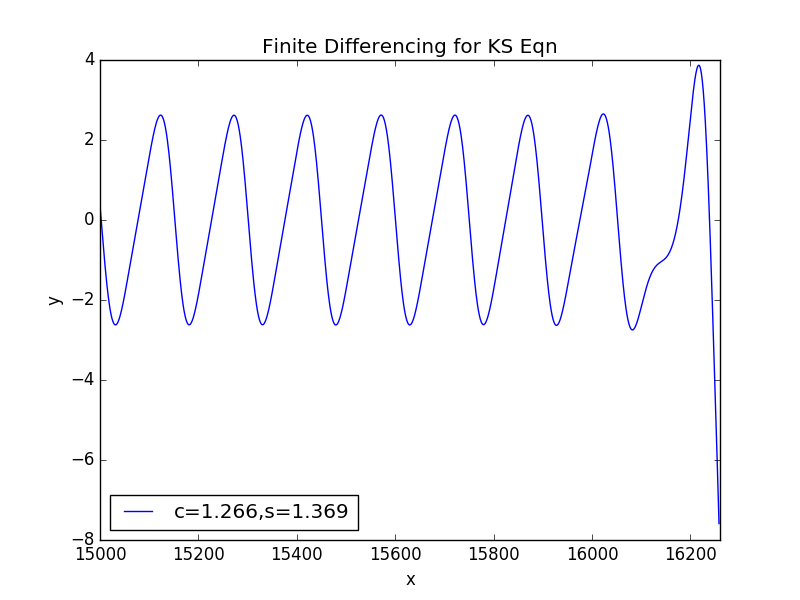
\includegraphics[scale=0.5]{ACxyplotc1266s1369a.png}
  \caption{
$(xy)$ plot. The trajectory generated through a finite difference scheme
outlined in Michelson\rf{Mks86} for $c=1.266$ and $s=1.369$.
  }

  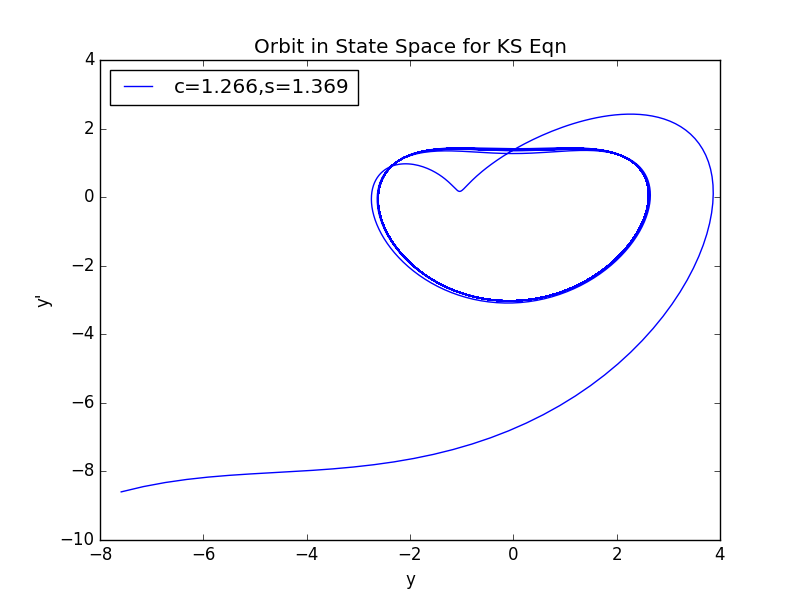
\includegraphics[scale=0.5]{ACorbitc1266s1369a.png}
  \caption{\Statesp\ plot. The near-periodic orbit generated through a finite difference
  scheme outlined in Michelson\rf{Mks86} for $c=1.266$ and $s=1.369$.}
\end{figure}
}


\item[2016-01-12 PC]  Literature
related to Michelson\rf{Mks86}:

Carmona \etal\rf{CFGT15}
{\em Noose structure and bifurcations of periodic orbits in reversible
three-dimensional piecewise linear differential systems}

Barker \etal\rf{BJNRZ12}
{\em Stability of periodic { Kuramoto-Sivashinsky} waves}

Aderogba, A. A. and Chapwanya, M. and Djoko\rf{AdChDj12}
{\em Travelling wave solution of the {Kuramoto-Sivashinsky} equation: A
computational study}


Dumortier,  Ibanez  and Kokubu\rf{DuIbKo06}
{\em Cocoon bifurcation in three-dimensional reversible vector fields}

Heidel and Zhang\rf{HeiZha07}
{\em Nonchaotic and chaotic behavior in three-dimensional quadratic systems:
{Five}-one conservative cases},

Nickel\rf{Nickel07}
{\em Travelling wave solutions to the {Kuramoto–Sivashinsky} equation }

Blomgren, Gasner, and Palacios\rf{BlGaPa05}
{\em Hopping behavior in the Kuramoto–Sivashinsky equation}
seems to be specific to $2D$: `` numerical `hopping' cellular flame
patterns are characterized by nonuniform rotations of a ring of cells, in
which individual cells make abrupt changes in their angular positions
while they rotate around the ring. Until now, these states have been
observed only in experiments but not in truly two-dimensional computer
simulations. A modal decomposition analysis of the simulated patterns,
via the proper orthogonal decomposition, reveals spatiotemporal behavior
in which the overall temporal dynamics is similar to that of equivalent
experimental states but the spatial dynamics exhibits a few more features
that are not seen in the experiments.
''


Dumortier,  Ibanez  and Kokubu\rf{DuIbKo06}
{\em Cocoon bifurcation in three-dimensional reversible vector fields}

Rempel \etal\rf{RCMR04}
{Analysis of chaotic saddles in high-dimensional dynamical systems: the
{Kuramoto-Sivashinsky} equation}: ``
study the role played by nonattracting chaotic sets called chaotic
saddles in chaotic transitions of high-dimensional dynamical systems. Our
methodology is applied to the Kuramoto-Sivashinsky equation. The paper
describes a novel technique that uses the stable manifold of a chaotic
saddle to characterize the homoclinic tangency responsible for an
interior crisis, a chaotic transition that results in the enlargement of
a chaotic attractor. The numerical techniques explained here are
important to improve the understanding of the connection between
low-dimensional chaotic systems and spatiotemporal systems which exhibit
temporal chaos and spatial coherence.''

Wilczak\rf{Wilczak03}
{\em Chaos in the {Kuramoto-Sivashinsky} equations -- a computer-assisted proof}

Strauss and Wang\rf{StrWan02}
 {\em Instability of traveling waves of the {Kuramoto-Sivashinsky} equation}

Ishimura\rf{Ishimura02}
{\em Remarks on third-order {ODEs} relevant to the {Kuramoto-Sivashinsky} equation}

Ishimura and Nakamura\rf{IshNak00}
{\em Nonexistence of monotonic solutions of some third-order ode relevant
to the {Kuramoto-Sivashinsky} equation}

Wittenberg and Holmes\rf{witt99hol}
{\em Scale and space localization in the {Kuramoto-Sivashinsky} equation}:
  ``
Using a wavelet basis, the spatiotemporally chaotic regime of the
    KSe is explored where a good seperation of scales is observed. In
    large scales, the dynamics is Gaussian. In the intermediate scales,
    the dynamics is reminiscent of travelling waves and heteroclinic
    cycles which is the typical behavior for small system size. In the
    small scales, the dynamics is intermittent. Through investigation
    of the interaction between different scales, we see the intermediate
    structures give the defining shape of the cell and the large scales
    trigger the spatiotemporal chaos. The small scales dissipate energy
    and modify the background in a average sense.

Yang\rf{ksyang97}
{\em On travelling-wave solutions of the {Kuramoto-Sivashinsky} equation}


Lau\rf{lau92}
{\em The cocoon bifurcations in three-dimensional systems with two fixed points}

Jones, Troy and MacGillivary\rf{kstroy92}
{\em Steady solutions of the {Kuramoto-Sivashinsky} equation for small wave speed}

Grimshaw and Hooper\rf{ksgrim91}
{\em The non-existence of a certain class of travelling wave solutions of
the {Kuramoto-Sivashinsky} equation},

Troy\rf{kstroy89}
{\em The existence of steady solutions of the {Kuramoto-Sivashinsky} equation}

Hooper and Grimshaw\rf{kshooper88}
{\em Travelling wave solutions of the {Kuramoto-Sivashinsky} equation}

Stanislavova and Stefanov\rf{StaSte11}
{\em Asymptotic estimates and stability analysis of {Kuramoto-Sivashinsky}
type models}

\end{description}

\subsection{Dong and Lan / DoLa14}
\label{sect:DoLa14}
Dong and Lan\rf{DoLa14}
{\em Organization of spatially periodic solutions of the steady
{Kuramoto-Sivashinsky} equation}

\begin{description}

\MNGpost{2017-07-17}{
{\bf DoLa14}
The goal of Dong and Lan\rf{DoLa14}
% {\em Organization of spatially
% periodic solutions of the steady {Kuramoto-Sivashinsky} equation}
is to
formulate a systematic way to locate periodic orbits with variational
method developed by Lan  and Cvitanovi{\'c}\rf{CvitLanCrete02,lanVar1},
as well as develop symbolic dynamics to classify these periodic orbits.
    }

\item[2013-12-29 PC] Dong and Lan\rf{DoLa14} study \eqva\ of \KS\ at $L
    = 43.5$. Previous system sizes were  was for antisymmetric
    subspace, system size $ \tildeL = 2.89109$ in
    \refref{Christiansen97}, $L = 38.5$ in \refref{lanCvit07}, $L =
    40.95$ in Lan~\etal\rf{LCC06}, and full \statesp\ $L=22$ in
    \refref{SCD07}. Dong and Lan continue the discussion of Lan's
    \HREF{http://www.cns.gatech.edu/~y-lan/thesis/thesis.pdf}
    {thesis}\rf{LanThesis}. Only \eqva, no mention of \reqva.

They credit Troy\rf{kstroy89,kstroy92} and Greene \& Kim\rf{ksgreene88}
with first studies of \KS\ \eqva.

\ACpost{2017-11-01}{{\bf DoLa14}
Reading this paper's introduction and background tremendously helped me understand
the \KSe\ more.
\begin{equation}
    u_t = (u^2)_x - u_{xx} - \nu u_{xxxx}
\end{equation}
The first derivative term is responsible for the interactions
between spatial modes at different scales (assuming this means length scales $L$)
and transfers energy from the low wavenumber modes to the higher ones. The second
term pumps energy into the system and makes it unstable at large scales while the
third term dissipates energy and damps at small scales.

Matt has gone over the spectral decomposition of the solution many times, but I
will just repeat it here for reference: using the form
\begin{equation}
    u(x,t) = i \sum_{k=-\infty}^{+\infty} a_k(t) e^{ikqx} \qquad \text{where } q = 2\pi/L,
\end{equation}
we can obtain an infinite ladder of coupled ODEs
\begin{equation}
    \dot{a}_k = [(kq)^2 - \nu (kq)^4] a_k - kq \sum_{m=-\infty}^{+\infty} a_m a_{k-m}.
\end{equation}
Since the dissipation term $\nu (kq)^4$ dominates for large wavenumber components, these
terms will not be excited enough significantly contribute to the dynamics. Thus, we can
truncate the set of ODEs such that $a_k = 0$ for $|k|>N$. In most cases, we take $N = 16$.
For small $L$, all Fourier modes are linearly stable, but the system quickly becomes
increasingly turbulent once $L$ increases by a significant amount.

From the video that Predrag recommended as well as the paper, the \KSe\ can be written as
\begin{align}
    &u^2 - u_x - \nu u_{xxx} = c\\
    &\implies \left\{
    \begin{array}{l}
	u_x = v\\
	v_x = w\\
	w_x = u^2 - v - c
    \end{array}
    \right.\\
    &\implies (u+w)_x = u^2 - c
\end{align}
We can see that $u+w$ increases without bound when $c<u^2$. When $c>u^2$ we can find
attractors appear in the state space. However, something weird happens when $c = u^2$
such that the derivative on the left side of Eqn 4.10 equals 0: both an attractor and
repeller appear in the state space, and it seems that trajectory enters the sink and
reappears at the source (if I'm understanding Predrag's drawing in the video correctly).

I'm still working through the variational methods part of the paper to see what they
actually did with the numerical simulations. So far, it seems that there exists four
simple building blocks for creating allowable orbits. This numbering notation reminds
me of the billiard (or pinball) orbit example that was covered in the Group Theory
class.
}

\item[2013-12-29 PC] we still have to study
Dong and Y. Lan\rf{DoLa14a}
{\em A variational approach to connecting orbits in nonlinear dynamical systems }

\end{description}

`` At fixed system size $L =43.5$, important equilibria
      are identified and shown to organize the dynamics. The first
      integral of the steady KSe leads to a 3D dynamical system with an
      integration constant $c$. At a typical value of $c = 0.40194$, four
      simplest cycles are identified and used as basic building blocks to
      construct longer cycles. The symbolic dynamics based on trajectory
      topology are very effective in classifying all short periodic
      orbits. The the return map on a chosen {\PoincSec} shows the
      complexity of the dynamics and the bifurcation of building blocks
      provides a chart to look for possible cycles at given periods. ''

The $n$ cell state\rf{FSTks86} is stable in finite windows for
arbitrarily large system sizes.

``
the antisymmetric heteroclinic orbit $\in \bbU^+$ connecting the two \eqva\ in
(9) is the only bounded nonconstant solution when the integration
constant $c\to\infty$\rf{mcord86}. For $c$ large enough, the heteroclinic
orbit remains the unique bounded solution\rf{Mks86}. It continues to be
numerically observable with $c$ down to 0.07\rf{kshooper88}, and was
computed analytically with normal form analysis for $c\ll
1$\rf{kschang86}. When $c$ decreases from large values, new connections
with more zeroes are born through saddle-node bifurcations until one
periodic orbit emerges as a limit of the connecting orbit with infinite
number of zeros. Bifurcation analysis with spatial Fourier modes gives
interesting features of spatially periodic steady solutions in certain
parameter regime\rf{ksgreene88}.
''

%%%%%%%%%%%%%%%%%%%%%%%%%%%%%%%%%%%%%%%%%%%%%%%%
%\printbibliography[heading=subbibintoc,title={References}]

The next benefit is not due to the inclusion of new methods but
rather the exclusion of old methods. Time integration and
recurrence functions based on pairwise distance have long been used in combination
to find initial conditions. % schatz/grigoriev, kerswell, viswanath.
In the high dimensional limit, both
of these components are time consuming. This is yet another
component of the dynamical systems formulation that gets worse
as spatial sizes increase. There are two detrimental factors
that contribute towards this. The number of dimensions must increase
in order to accurately resolve the domain. The other factor is that
the growth of complexity of solutions can reduce the number of recurrences
drastically. There isn't really a manner to deal with the increasing
number of computational variables other than to wait for improvements
in computing power and memory availability. As for the recurrences, the
typical solution for increasingly rare events is to compute in parallel when
possible. The exponential growth in complexity makes even this proposition
a daunting one.

% The italicized text captures my sentiment of this next paragraph.
The \spt\ completely avoids this by constructing larger \twots\
from the combination of smaller \twots. That is,
we locate the fundamental tiles, which are easy to find due to their small
domain size, and then build them up to create larger \twots. The only
search required is the search for the fundamental tiles. To stress
this even further \textit{one of the challenges of turbulence
computations has been eliminated}. The reason
why the search for the fundamental tiles is classified as ``easy'' is because
in the small domain size limit there just aren't that many \twots; the dynamics
is relatively simple.

% I'm trying to say that the arbitrary choice of norm is not as impactful in our case....
Recurrence functions also require the introduction of a norm,
typically chosen without taking the geometry of the state space into account.
Points that are close in this norm can be far apart in a dynamical sense (\ie, on opposite sides
of an unstable manifold). An arbitrary norm is also chosen in the \spt\
context but there are some subtle differences. For starters, the
norm introduced in the \spt\ formulation is not beholden to dynamics, as
there are no longer any dynamics to speak of.
Additionally, the norm in the \spt\ case measures the distance between \twots,
not just single state space points. This is not a statement of proof but rather
a suggestion that the underlying topology improves the reliability of
the chosen norm. Restated in a different manner, the \spt\ norm
takes both the magnitude and phase into account.

Conventional methods treat spatial dimensions
as finite and fixed; meanwhile, time is treated as infinite.
One interpretation is that this is natural due to the
human familiarity with finite space, especially in regards
to experimental setups.
This assumption is actually a very unnatural one
in the context of state space. The fundamental reason
for this is that it disregards
the translational invariance of the equations and while there
are implicit physical scales, choosing a specific domain size
to study is completely arbitrary. This notion
must be reconsidered going forward as it is a very strict constraint
on the space of solutions and on the study of turbulence in general.
Finite spatial dimensions of course have practical import, but
these specific constraints should only be imposed after the
study of infinite space-time, as they represent special
cases of the general equations. The \spt\ formulation handles
this properly by treating all continuous dimensions as equal
by respecting all translational symmetries.
What are the differences and advantages of this?
The first key difference is that the governing equation
dictates the \spt\ domain size in an unsupervised
fashion; the decision of what specific domain size
to study is no longer present in the discussion.
This is another manner in which
time and space are being treated as equals; the parameters $(L,T)$
that determine the size of the \spt\ domain are both allowed to vary.
The values of these parameters
are determined by the requirement that the equations
must be satisfied locally at every lattice site.
This small detail, allowing the domain size $L$ to vary,
is not as trivial as it seems. At present it has not been seen in
the dynamical systems literature. The variation of the period $T$ is
common, however. The likely culprit behind this different treatment
is likely a result of the equations themselves. This difficulty
is especially evident in the \KSe, whose spatial derivative terms
are of higher order than the first order time derivative, but also
there is a spatial derivative present in the nonlinear component.


    The conventional method to generate initial conditions
involves time integration and recurrence functions, the latter simply
calculates the pairwise distance between all points in a time integrated
series.%schatz/grigoriev, kerswell, viswanath.
In the high dimensional limit, both
of these components are time consuming. This is yet another
component of the dynamical systems formulation that gets worse
as spatial sizes increase. There are two detrimental factors
that contribute towards this. The number of dimensions must increase
in order to accurately resolve the domain. The other factor is that
the growth of complexity of solutions can reduce the number of recurrences
drastically. There isn't really a manner to deal with the increasing
number of computational variables other than to wait for improvements
in computing power and memory availability. As for the recurrences, the
typical solution for increasingly rare events is to compute in parallel when
possible. The exponential growth in complexity makes even this proposition
a daunting one.

The \spt\ completely avoids this by constructing larger \twots\
from the combination of smaller \twots. That is,
we locate the fundamental tiles, which are easy to find due to their small
domain size, and then build them up to create larger \twots. The only
search required is the search for the fundamental tiles. To stress
this even further \textit{one of the challenges of turbulence
computations has been eliminated}. The reason
why the search for the fundamental tiles is classified as ``easy'' is because
in the small domain size limit there just aren't that many \twots; the dynamics
is relatively simple.

Recurrence functions also require the introduction of a norm,
typically chosen without taking the geometry of the state space into account.
Points that are close in this norm can be far apart in a dynamical sense (\ie, on opposite sides
of an unstable manifold). An arbitrary norm is also chosen in the \spt\
context but there are some subtle differences. For starters, the
norm introduced in the \spt\ formulation is not beholden to dynamics, as
there are no longer any dynamics to speak of.
Additionally, the norm in the \spt\ case measures the distance between \twots,
not just single state space points. This is not a statement of proof but rather
a suggestion that the underlying topology improves the reliability of
the chosen norm. Restated in a different manner, the \spt\ norm
takes both the magnitude and phase into account.
Another numerical advantage is that the \spt\ formulation is able to find solutions
of the \KSe\ starting from modulated random noise. The specifics
of ``modulated random noise'' are described in the numerical methods section
but it can essentially be thought of as randomly assigning values to \spt\
Fourier modes. The ability to find solutions from this starting point
is a radical improvement over the conventional capabilities. This is of course
in conjunction with allowing the \spt\ domain to change. The reaction to these
changes individually has induced skepticism and disbelief; together they comprise
a completely unheard of force.

The \spt\ formulation also includes the improvement of a commonly
practiced numerical method known as pseudo-arclength continuation.
The general idea is to track a solution as a parameter is varied. In the
Navier-Stokes equations this is typically the Reynolds number.
The improvement is due to our common refrain: the lack of dynamical
instability and the topological constraint of \twots. There can
be more confidence that if the continuation fails it is due to the solution
not existing rather than not being able to converge due to dynamical instability.

\section{\KSe}
% KSe.tex
% $Author: siminos $ $Date: 2009-10-05 16:13:22 -0400 (Mon, 05 Oct 2009) $

\section{\KSe}
\label{s-KS}

The \KS\ [henceforth KS] system\rf{ku,siv},
which arises in the description of
stability of flame fronts, reaction-diffusion systems and many other
physical settings\rf{KNSks90}, is one of the simplest nonlinear PDEs that
exhibit spatiotemporally chaotic behavior. In the formulation
adopted here, the time evolution of the `flame front velocity'
$u=u(x,t)$ on a periodic domain $u(x,t) = u(x+L,t)$ is given by
\beq
  u_t = F(u) = -{\textstyle\frac{1}{2}}(u^2)_x-u_{xx}-u_{xxxx}
    \,,\qquad   x \in [-L/2,L/2]
    \,.
\ee{ks}
Here $t \geq 0$ is the time, and $x$ is the spatial coordinate.
The subscripts $x$ and $t$ denote partial derivatives with respect to
$x$ and $t$. In what follows
we shall state results of all calculations either in units of the
`dimensionless system size' $\tildeL$, or the system size $L = 2 \pi
\tildeL$. \refFig{f:ks_largeL} presents a typical `turbulent' evolution
for KS. All numerical results presented in this paper
are for the system size $\tildeL=22/2\pi = 3.5014\ldots$, for which a
structurally stable chaotic attractor is observed (see \reffig{f:ks_L22}).
Spatial periodicity $u(x,t)=u(x+L,t)$
makes it convenient to work in the Fourier space,
\beq
  u(x,t)=\sum_{k=-\infty}^{+\infty} a_k (t) e^{ i k x /\tildeL }
\,,
\ee{eq:ksexp}
with the $1$-dimensional PDE \refeq{ks}
replaced by an infinite set of
ODEs for the complex Fourier coefficients $a_k(t)$:
\beq
\dot{a}_k= \pVeloc_k(a)
     = ( q_k^2 - q_k^4 )\, a_k
    - i \frac{q_k}{2} \sum_{m=-\infty}^{+\infty} a_m a_{k-m}
\,,
\ee{expan}
where $q_k = k/\tildeL$.
Since $u(x,t)$ is real, $a_k=a_{-k}^\ast$, and we can replace the
sum by an $m > 0$ sum.

Due to the hyperviscous damping $u_{xxxx}$, long time solutions of KS
equation are smooth, $a_k$ drop off fast
with $k$, and truncations of \refeq{expan} to $16 \leq N \leq 128$
terms yield accurate solutions for system sizes considered here (see
\refappe{sec:fourierRLD}).  Robustness of the long-time dynamics
of KS as a function of the number of Fourier modes kept in truncations
of \refeq{expan} is, however, a subtle issue.  Adding an extra mode to
a truncation of the system introduces a small perturbation in the
space of dynamical systems.  However, due to the lack of structural
stability both as a function of truncation $N$, and the system size
$L$, a small variation in a system parameter can (and often will)
throw the dynamics into a different asymptotic state.  For example,
asymptotic attractor which appears to be chaotic in a $N$-dimensional
\statesp\ truncation can collapse into an attractive cycle
for $(N\!+\!1)$-dimensions.
Therefore, the selection of parameter $L$ for which a
structurally stable chaotic dynamics exists and can be
studied is rather subtle. We have found that the value of $L
= 22$ studied in \refsect{sec:L22} satisfies these
requirements. In particular, all of the equilibria and
relative equilibria persist and remain unstable when $N$ is
increased from 32 (the value we use in our numerical
investigations) to 64 and 128.  Nearly all of the \rpo s we
have found for this system also exist and remain unstable for
larger values of $N$ as well as smaller values of the
integration step size (see \refappe{sec:lmderRLD} for
details).

%%%%%%%%%%%%%%%%%%%%%%%%%%%%%%%%%%%%%%%%%%%%%%%%%%%%%%%%%%%%%%
\begin{figure}[t]
\begin{center}
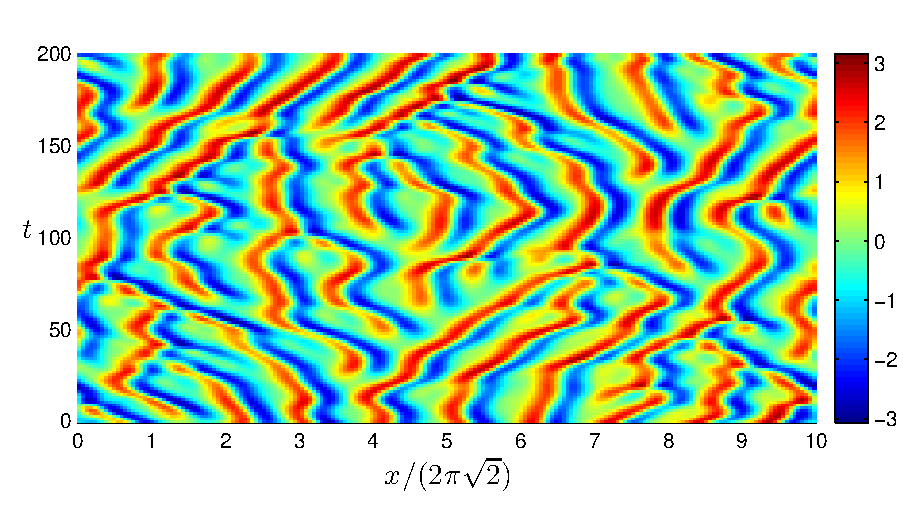
\includegraphics[width=0.9\textwidth]{figs_bmp/ks_largeL_cbar_200.eps} 
\end{center}
\caption{
A typical spatiotemporally chaotic solution of the \KSe, system size
$L=20\pi\sqrt{2}\approx 88.86$.  The $x$ coordinate is scaled
with the most unstable wavelength $2\pi\sqrt{2}$, which is
approximately also the mean wavelength of the turbulent flow.
The color bar indicates the color scheme for $u(x,t)$, used also
for the subsequent figures of this type.
     } \label{f:ks_largeL}
\end{figure}
%%%%%%%%%%%%%%%%%%%%%%%%%%%%%%%%%%%%%%%%%%%%%%%%%%%%%%%%%%%%%%%%%%

\subsection{Symmetries of \KSe}
\label{sec:KSeSymm}

The KS equation is Galilean invariant: if $u(x,t)$ is a solution,
then $u(x -ct,t) -c $, with $c$ an arbitrary constant
speed, is also a solution. Without loss of generality, in our
calculations we shall set the mean velocity of the front to zero,
\beq \int dx \, u = 0 \,. \ee{GalInv}
As $\dot{a_0}=0$ in
\refeq{expan}, $a_0$ is a conserved quantity
fixed to $a_0=0$ by the condition \refeq{GalInv}. $G$, the group of actions $ g \in G $ on a
\statesp\ (reflections, translations, \etc) is a symmetry of the KS
flow \refeq{ks} if $g\,u_t = F(g\,u)$.
The KS equation is time translationally invariant, and space translationally invariant
on a periodic domain under
the 1-parameter group of
$O(2): \{\Shift_{\shift/L},\Refl \}$.
If $u(x,t)$ is a solution, then
$\Shift_{\shift/L}\, u(x,t) = u(x+\shift,t)$
is an equivalent solution for any shift
$-L/2 < \shift \leq L/2$,
as is the
reflection (`parity' or `inversion')
\beq
    \Refl \, u(x) = -u(-x)
\,.
\ee{KSparity}
The translation operator action on the Fourier coefficients \refeq{eq:ksexp},
represented here by a complex valued vector
$a = \{a_k\in\mathbb{C}\,|\,k = 1, 2, \ldots\}$, is given by
\beq
  \Shift_{\shift/L}\, a = \mathbf{g}(\shift) \, a \,,
  \label{eq:shiftFour}
\eeq
where $\mathbf{g}(\shift) = \diag( e^{i q_k\, \shift} )$ is a complex
valued diagonal matrix, which amounts to the $k$-th mode complex plane
rotation by an angle $k\, \shift /\tildeL$.  The reflection acts on
the Fourier coefficients by complex conjugation,
\beq
  \Refl \, a = -a^\ast
\,.
\ee{FModInvSymm}
Reflection generates the dihedral subgroup $D_1 = \{1, \Refl\}$
of $O(2)$.  Let $\bbU$ be the space of
real-valued velocity fields periodic and square integrable
on the interval $\Omega = [-L/2,L/2]$,
\begin{align}
 \bbU  &= \{u \in L^2(\Omega) \; | \; u(x) = u(x+L)\}  \,.
\end{align}
A continuous symmetry maps each state $u \in \bbU$
to a manifold of functions with identical dynamic behavior.
Relation $\Refl^2 = 1$ induces linear decomposition
$u(x) = u^+(x)+ u^-(x)$,
$u^\pm(x)= P^\pm u(x) \in  \bbU^\pm$,
into irreducible subspaces
$
\bbU = \bbU^+
       \oplus \bbU^-
$, where
\beq
    P^+=(1+\Refl)/2
    \,,\qquad
    P^-=(1-\Refl)/2
\,,
\ee{P1P2proj} are the antisymmetric/symmetric projection operators.
Applying $P^+,\,P^-$ on the KS equation \refeq{ks} we have\rf{KNSks90}
\bea
 u_t^+ &=& - (u^+u^+_x + u^-u^-_x )
                - u^+_{xx} - u^+_{xxxx}
    \continue
 u_t^- &=& - (u^+u^-_x + u^-u^+_x )
                - u^-_{xx} - u^-_{xxxx}
\,.
\label{KSD1}
\eea
If $u^- = 0$, KS flow is confined to
the antisymmetric $\bbU^+$ subspace,
\beq
 u_t^+ = - u^+u^+_x
                - u^+_{xx} - u^+_{xxxx}
\,,
\label{KSU+}
\eeq
but otherwise the nonlinear terms in \refeq{KSD1}
mix the two subspaces.

Any rational shift $ \Shift_{1/m}u(x)=u(x+L/m)$ generates a discrete
cyclic subgroup $C_m$ of $O(2)$, also a symmetry of KS
system. Reflection together with $C_m$ generates another
symmetry of KS system, the dihedral subgroup $D_m$ of $O(2)$.
The only non-zero Fourier components of a solution invariant
under $C_m$ are $a_{jm} \neq 0$, $j =1,2,\cdots$, while for a
solution invariant under $D_m$ we also have the condition
$\Re a_j=0$ for all $j$.
$D_m$ reduces the dimensionality of \statesp\ and aids computation of
\eqva\ and \po s within it. For example, the 1/2-cell translations \beq
    \Shift_{1/2}\, u(x)=u(x+L/2)
\ee{KSshift}
and reflections generate $O(2)$
subgroup $D_2 = \{1, \Refl,\Shift,\Shift\Refl\}$,
which
reduces the \statesp\ into four irreducible subspaces
(for brevity, here $\Shift = \Shift_{1/2}$):
\begin{align}
 & \qquad\qquad\qquad\qquad\qquad
              ~~~ \Shift ~~ \Refl  ~\;  \Shift\Refl
    \nnu\\
P^{(1)} &= \frac{1}{4} (1 + \Shift + \Refl + \Shift\Refl)
           ~~~~  S  ~~  S   ~~   S
    \nnu\\
P^{(2)} &= \frac{1}{4} (1 + \Shift - \Refl - \Shift\Refl)
            ~~~~  S  ~~  A   ~~   A
    \nnu\\
P^{(3)} &= \frac{1}{4} (1 - \Shift + \Refl - \Shift\Refl)
           ~~~~  A  ~~  S   ~~   A
     \label{ek_defn}\\
P^{(4)} &= \frac{1}{4} (1 - \Shift - \Refl + \Shift\Refl)
          ~~~~  A  ~~  A   ~~   S
\,.
    \nnu
\end{align}
$P^{(j)}$ is the projection operator onto
$u^{(j)}$ irreducible subspace, and the last 3 columns
refer to the symmetry (or antisymmetry) of
$u^{(j)}$ functions under reflection and
1/2-cell shift.
By the same argument that identified \refeq{KSU+} as
the invariant subspace of KS, here the KS flow
stays within the
 $\bbU^S =  \bbU^{(1)}+ \bbU^{(2)}$
irreducible $D_1$ subspace of
$u$ profiles symmetric under 1/2-cell shifts.

While in general the bilinear term $(u^2)_x$  mixes the
irreducible subspaces of $D_n$, for $D_2$ there are
four subspaces invariant under the flow\rf{KNSks90}:
\begin{romannum}
 \item[$\{0\}$:~~~~~~] the $u(x)=0$ {\eqv}
 \item[$\bbU^+ = \bbU^{(1)}+ \bbU^{(3)} $:]
    the reflection $D_1$ irreducible space of antisymmetric $u(x)$
 \item[$\bbU^S =  \bbU^{(1)}+ \bbU^{(2)}$:]
    the shift $D_1$ irreducible space of $L/2$ shift symmetric  $u(x)$
 \item[$\bbU^{(1)}$:~~~~~]
    the $D_2$ irreducible  space of $u(x)$ invariant under $x\mapsto L/2-x,\ u\mapsto -u$.
\end{romannum}
With the continuous
translational symmetry eliminated within each subspace, there are no
\reqva\ and \rpo s, and one
can focus on the \eqva\ and \po s only, as was done
for $\bbU^+$ in \refrefs{Christiansen97,LanThesis,lanCvit07}.
In the Fourier
representation, the
$u \in \bbU^+$
antisymmetry amounts to having purely imaginary
coefficients, since $a_{-k}= a^\ast_k = -a_k$.
The 1/2 cell-size shift $\Shift_{1/2}$
generated 2-element discrete subgroup
$\{1,\Shift_{1/2}\}$ is
of particular interest
because in the $\bbU^+$ subspace the translational invariance of the full system reduces to
invariance under discrete translation \refeq{KSshift} by half a
spatial period $L/2$.

Each of the above dynamically invariant subspaces is unstable
under small perturbations, and generic solutions of \KSe\ belong to
the full space.
Nevertheless, since  all \eqva\ of the KS flow studied in this paper
lie in the $\bbU^+$ subspace (see
\refsect{sec:L22}), $\bbU^+$  plays important role for the global
geometry of the flow.
The linear stability matrices of these \eqva\ have
eigenvectors both in and outside of $\bbU^+$, and need to be
computed in the full \statesp.




\subsection{\Eqva\ and \reqva}
\label{sec:stks}

\Eqva\  (or the steady solutions)
are the fixed profile time-invariant solutions,
\beq
 u(x,t) = u_\stagn(x)
\,.
\ee{eqva}
Due to the translational symmetry,
the KS system also allows for
\reqva\ (traveling waves, rotating waves),
characterized by a fixed profile $u_\stagn(x)$
moving with constant speed $c$, {\ie}
\beq
 u(x,t) =  u_\stagn(x-ct)
\,.
\ee{reqva}
Here suffix ${}_\stagn$ labels a particular invariant solution.
Because of the reflection symmetry \refeq{KSparity},
the \reqva\ come in counter-traveling pairs
$u_\stagn(x-ct)$, $-u_\stagn(-x+ct)$.

The \reqv\ condition for the {\KS} PDE \refeq{ks}
is the ODE
\beq
{\textstyle\frac{1}{2}}(u^2)_x+u_{xx}+ u_{xxxx}=c \, u_x
\ee{KSeqvCond}
which can be analyzed as a dynamical system in its own right.
Integrating once we get
\beq
{\textstyle\frac{1}{2}}u^2 - c u + u_x + u_{xxx}=\expctE
\,.
\label{eq:stdks}
\eeq
This equation can be interpreted as a 3-dimen\-si\-on\-al dynamical system
with spatial coordinate $x$ playing the role of `time,'
and the integration constant \expctE\ can be interpreted as `energy,'
see \refsect{sec:energy}.

For $\expctE>0$ there is rich $\expctE$-dependent dynamics,
with fractal sets of bounded solutions investigated in depth
by Michelson\rf{Mks86}. For $\tildeL<1$ the only \eqv\ of the
system is the globally attracting constant solution
$u(x,t)=0$, denoted $\EQV{0}$ from now on. With increasing
system size $L$ the system undergoes a series of
bifurcations. The resulting \eqva\ and \reqva\ are described
in the classical papers of Kevrekidis, Nicolaenko and
Scovel\rf{KNSks90}, and Greene and Kim\rf{ksgreene88},
among others. The relevant bifurcations up to the
system size investigated here are summarized in
\reffig{fig:ksBifDiag}: at $\tildeL=22/2\pi = 3.5014\cdots$,
the {\eqva} are the constant solution \EQV{0},
the  \eqv\ \EQV{1} called GLMRT by Greene and
Kim\rf{laquey74,ksgreene88},
the $2$- and $3$-cell states
\EQV{2} and \EQV{3}, and the pairs of \reqva\ \REQV{\pm}{1},
\REQV{\pm}{2}.
All \eqva\ are in the antisymmetric subspace $\bbU^+$, while
\EQV{2} is also invariant under $D_2$ and \EQV{3} under
$D_3$.


%%%%%%%%%%%%%%%%%%%%%%%%%%%%%%%%%%%%%%%%%%%%%%%%%%%%%%%%%%%%%%%%
\begin{figure}[t]       \label{fig:ksBifDiag}
\begin{center}
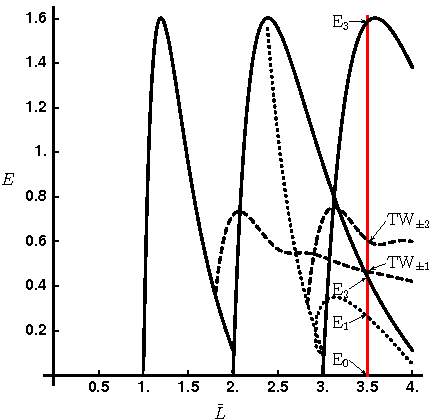
\includegraphics[width=0.5\textwidth]{figs_bmp/ksBifDiag_pst.eps}
\end{center}
\caption{
The energy \refeq{ksEnergy} of the \eqva\ and \reqva\ that
exist up to $L=22$, $\tildeL = 3.5014\ldots$, plotted as a function
of the system size $\tildeL = L/2\pi$ (additional \eqva, not present
at $L = 22$ are given in \refref{ksgreene88}). Solid curves denote
$n$-cell solutions \EQV{2} and \EQV{3}, dotted curves the GLMRT
\eqv\ \EQV{1},
and dashed curves the \reqva\ \REQV{\pm}{1} and \REQV{\pm}{2}.
The parameter $\alpha$ of \refrefs{KNSks90,ksgreene88} is
related to the system size by $\tildeL=\sqrt{\alpha/4}$.
        }
\end{figure}
%%%%%%%%%%%%%%%%%%%%%%%%%%%%%%%%%%%%%%%%%%%%%%%%%%%%%%%%%%%%%%%%%%

In the Fourier representation the \reqva\ time dependence is
\beq
 a_k(t) e^{-itc q_k} = a_k(0)
\,.
\ee{reqvaF}
Differentiating with respect to time, we obtain
the Fourier space version of the \reqv\ condition
\refeq{KSeqvCond},
\beq
 \pVeloc_k(a) - i q_k \velRel a_k = 0
\,,
\ee{reqvCondF}
which we solve for (time independent) $a_k$ and $c$.
Periods of spatially periodic {\eqva} are $L/n$ with integer $n$.
Every time the system size crosses  $\tildeL=n$,
$n$-cell states
are generated through pitchfork bifurcations off $u =0$
equilibrium.
Due to the translational invariance of {\KSe},
they form invariant circles
in the full \statesp.
In the $\bbU^+$ subspace considered here,
they correspond to $2n$ points, each shifted by $L/2n$.
For a sufficiently small $L$
the number of {\eqva} is small and
concentrated on the low wave-number end of the Fourier spectrum.

In a periodic box of size $L$
both \eqva\ and \reqva\ are  periodic solutions
embedded in 3-$d$ space, conveniently represented as loops in
$(u,u_x,u_{xx})$ space, see \reffig{f:KS22Equil}\,(\textit{d}).
In this representation the continuous translation symmetry
is automatic -- a rotation in the $[0,L]$ periodic domain only
moves the points along the loop. For an \eqv\ the points
are stationary in time; for \reqv\ they move in time, but in
either case, the loop remains invariant.
So we do not have the problem that we encounter in the Fourier
representation, where seen from the frame of one of the \eqva\
the rest trace out circles under the action of continuous symmetry
translations.

From \refeq{expan} we see that the origin $u(x,t) = 0$
has Fourier modes as the linear stability eigenvectors
(see \refappe{sec:stability}).  The $|k|<\tildeL$
long wavelength perturbations of the flat-front {\eqv}
are linearly unstable, while for
$|k|$ sufficiently larger than $\tildeL$ the short wavelength
perturbations are strongly contractive. The high $k$
eigenvalues, corresponding to rapid variations of the flame
front, decay so fast that the corresponding eigendirections
are physically irrelevant. Indeed, \refref{YaTaGiChRa08} shows that
the chaotic solutions of spatially extended dissipative
systems evolve within an inertial manifold spanned by a
finite number of physical modes, hyperbolically isolated from
a set of residual degrees of freedom with high $k$, themselves individually
isolated from each other.
The most unstable mode, nearest to $|k|=\tildeL/\sqrt{2}$,
sets the scale of the mean wavelength $\sqrt{2}$
of the KS `turbulent' dynamics,
see \reffig{f:ks_largeL}.


\subsection{\Rpo s, symmetries and \po s} \label{sec:KSePO}

The KS equation \refeq{ks} is time translationally invariant, and
space translationally invariant under the 1-$d$ Lie group of $O(2)$
rotations: if $u(x,t)$ is a solution, then $u(x+\shift,t)$ and
$-u(-x,t)$ are equivalent solutions for any $-L/2 < \shift \leq
L/2$.
As a result of invariance under $\Shift_{\shift/L}$,
KS equation can have \rpo\ solutions
with a profile $u_p(x)$, period $\period{p}$, and a
nonzero shift $\shift_p$
\beq
  \Shift_{\shift_p/L}u(x,\period{p}) =
  u(x+\shift_p,\period{p}) = u(x,0) = u_p(x)\,.
\label{KSrpos}
\eeq
{\Rpo s} \refeq{KSrpos} are periodic in
$\velRel_p=\shift_p/\period{p}$ co-rotating frame (see
\reffig{f:MeanVelocityFrame}), but in the stationary frame their
trajectories are quasiperiodic.  Due to the reflection symmetry
\refeq{KSparity} of KS equation, every {\rpo} $u_p(x)$ with shift
$\shift_p$ has a symmetric partner $-u_p(-x)$ with shift $-\shift_p$.

Due to invariance under reflections, KS equation can also have
\rpo s {\em with reflection}, which are
characterized by a profile $u_p(x)$ and
period $\period{p}$
\beq
  \Refl u(x+\shift,\period{p}) =
  -u(-x-\shift,\period{p}) = u(x+\shift,0) = u_p(x)
  \,,
\label{KSpos}
\eeq
giving the family of equivalent solutions
parameterized by $\shift$
(as the choice of the reflection point is arbitrary,
the shift can take any value in $-L/2 < \shift \leq L/2$).

Armbruster \etal\rf{AGHks89,AGHO288} and Brown and
Kevrekidis\rf{BrKevr96} (see also \refref{Krupa90}) link the
birth of \rpo s to an infinite period global bifurcation
involving a heteroclinic loop connecting equilibria or a
bifurcation of \reqva, and also report creation of \rpo\
branches through bifurcation of \po s.

As $\shift$ is continuous in the interval $[-L/2, L/2]$,
the likelihood of a \rpo\ with $\shift_p = 0$ shift is zero,
unless an exact periodicity is enforced by a discrete symmetry,
such as the dihedral symmetries discussed above.
If the shift $\shift_p$ of a \rpo\ with period $\period{p}$ is such
that $\shift_p /L$ is a rational number, then the orbit is
periodic with period $n\period{p}$.  The likelihood to find such \po s is
also zero.

However, due to the KS equation invariance under
the dihedral $D_n$ and cyclic $C_n$ subgroups, the following
types of \po s are possible:

{\bf (a)} The \po\ lies
within a subspace pointwise invariant under the action of
$D_n$ or $C_n$. For instance, for $D_1$ this is the
$\bbU^+$ antisymmetric subspace, $-u_p(-x) = u_p(x)$, and
$u(x,\period{p}) = u(x,0) = u_p(x)$. The periodic orbits
found in \refrefs{Christiansen97,lanCvit07} are
all in $\bbU^+$, as the dynamics is restricted to
antisymmetric subspace. For $L=22$ the dynamics in $\bbU^+$
is dominated by attracting (within the subspace)
heteroclinic connections and thus we have no periodic orbits
of this type, or in any other of the $D_n$--invariant
subspaces, see \refsect{sec:L22}.

{\bf (b)} The \po\ satisfies
\beq
	 u(x,t+\period{p})=\gamma u(x,t)\,,
	\label{eq:POspattemp}
\eeq
for some group element $\gamma\in O(2)$ such that
$\gamma^m=e$ for some integer $m$ so that the orbit repeats
after time $m \period{p}$ (see
\refref{golubitsky2002sp} for a general discussion of
conditions on the symmetry of a \po).
If an orbit is of reflection type \refeq{KSpos},
$\Refl\Shift_{\shift/L} u(x,\period{p}) =
-u(-x-\shift,\period{p}) = u(x,0)$, then it is pre-periodic
to a \po\ with period $2\period{p}$. Indeed, since
$(\Refl\Shift_{\shift/L})^2 = \Refl^2 = 1$, and the KS
solutions are time translation invariant, it follows from
\refeq{KSpos} that
\[
  u(x,2\period{p}) = \Refl\Shift_{\shift/L} u(x,\period{p}) =
  (\Refl\Shift_{\shift/L})^2 u(x,0) = u(x,0)\;.
\]
Thus any shift acquired during time $0$ to
$\period{p}$ is compensated by the opposite shift during
evolution from $\period{p}$ to $2 \period{p}$.
All periodic orbits we have found for $L=22$ are of type
\refeq{eq:POspattemp} with $\gamma=R$. Pre-periodic orbits
with $\gamma\in C_n$ have been found by Brown and
Kevrekidis\rf{BrKevr96} for KS system sizes larger than ours,
but we have not found any for $L=22$.
Pre-periodic orbits are a hallmark of any dynamical system
with a discrete symmetry, where they have a natural
interpretation as \po s in the fundamental
domain\rf{CvitaEckardt,DasBuch}.

\section{Energy transfer rates}
\label{sec:energy}

In physical settings where the observation times are much
longer than the dynamical `turnover' and Lyapunov times
(statistical mechanics, quantum physics, turbulence) periodic
orbit theory\rf{DasBuch} provides highly accurate predictions
of measurable long-time averages such as the dissipation and
the turbulent drag\rf{GHCW07}. Physical predictions have to
be independent of a particular choice of ODE representation
of the PDE under consideration and, most importantly,
invariant under all symmetries of the dynamics. In this
section we discuss a set of such physical observables for the
1-$d$ KS invariant under reflections and translations. They
offer a representation of dynamics in which the symmetries
are explicitly quotiented out. We shall use these
observables in \refsect{sec:energyL22} in order to
visualize a set of solutions on these coordinates.

The {space average} of a function $\obser = \obser(\pSpace,t) = \obser(u(x,t))$  on
the interval $L$,
\beq
    \expct{\obser} = \Lint{\pSpace}\, \obser(\pSpace,t)
    \,,
    \label{rpo:spac_ave}
\eeq
is in general time dependent.
Its mean value is given by the {time average}
\beq
\timeAver{\obser}
    =
\lim_{t\rightarrow \infty} \frac{1}{t} \int_0^t \! d\tau \, \expct{\obser}
    =
\lim_{t\rightarrow \infty} \frac{1}{t} \int_0^t \!
    \Lint{\tau}  d\pSpace\, \obser(\pSpace,\tau)
    \,.
\label{rpo:tim_ave}
\eeq
The mean value of $\obser = \obser(u_\stagn) \equiv \obser_\stagn$ evaluated on
\eqv\ or {\reqv} $u(\pSpace,t) = u_\stagn(\pSpace-ct)$, labeled by  $q$ as in 
\refeq{reqva}, is
\beq
\timeAver{\obser}_\stagn = \expct{\obser}_\stagn = \obser_\stagn\,.
\label{rpo:u-eqv} \eeq 
Evaluation of the infinite time average
\refeq{rpo:tim_ave} on a function of a \po\ or \rpo\
$u_p(\pSpace,t)=u_p(\pSpace+\shift_p,t+\period{p})$ requires only a single
$\period{p}$ traversal,
\beq
  \timeAver{\obser}_p = \frac{1}{\period{p}}
    \int_0^{\period{p}} \! d\tau \, \expct{\obser}
\,.
\label{rpo:u-cyc}
\eeq

Equation \refeq{ks} can be written as
\beq
    u_t=- V_x
        \,,\qquad
    V(x,t)={\textstyle\frac{1}{2}}u^2+u_{x} + u_{xxx}
    \,.
\ee{ksPotent}
If $u$ is `flame-front velocity' then \expctE, defined in
\refeq{eq:stdks}, can be interpreted as the mean energy
density. So, even though KS is a phenomenological
small-amplitude equation, the time-dependent $L^2$ norm
of $u$,
\beq
    \expctE=
  \Lint{\pSpace}
  V(x,t)=
  \Lint{\pSpace} \frac{u^2}{2}
  \,,
  \label{ksEnergy}
\eeq
has a physical interpretation\rf{ksgreene88} as the average `energy'
density of the flame front. This analogy to the mean kinetic energy
density for the Navier-Stokes motivates what follows.

The energy \refeq{ksEnergy} is intrinsic to the flow,
independent of the particular ODE basis set chosen to
represent the PDE. However, as the Fourier amplitudes are
eigenvectors of the translation operator, in the Fourier
space the energy is a diagonalized quadratic norm,
\beq
\expctE
          =  \sum_{k=-\infty}^{\infty} E_k
\,,\qquad
E_k =
    {\textstyle\frac{1}{2}}|a_k|^2
\,,
\ee{EFourier}
and explicitly invariant term by term
under translations
\refeq{eq:shiftFour}
and reflections \refeq{KSparity}.

Take time derivative of the energy density \refeq{ksEnergy},
substitute \refeq{ks} and integrate by parts. Total derivatives vanish
by the spatial periodicity on the $L$ domain:
\bea
   \dot{\expctE} &=&
     \expct{u_t \, u}
         = - \expct{\left({u^2}/{2} + u_{x} + u_{xxx}\right)_x u }
    \continue
    &=&
\expct{ u_x \, {u^2}/{2} + u_{x}^2 + u_x \, u_{xxx}}
    \,.
\label{rpo:ksErate}
\eea
The first term in \refeq{rpo:ksErate} vanishes by
integration by parts,
\(
3 \expct{ u_x \, u^2}= \expct{(u^3)_x} = 0
\,,
\)
and integrating the third term by parts yet again
one gets\rf{ksgreene88} that the energy variation
\beq
   \dot{\expctE} = P - D
                \,,\qquad
      P =  \expct{u_{x}^2}
                \,,\quad
      D =  \expct{u_{xx}^2}
\ee{EnRate}
balances the power $P$ pumped in by anti-diffusion $u_{xx}$
against the energy dissipation rate $D$
by hyper-viscosity $u_{xxxx}$
in the KS equation \refeq{ks}.

The time averaged energy density  $\timeAver{E}$
computed on a typical orbit goes to a constant, so
the mean values \refeq{rpo:tim_ave} of drive and dissipation
exactly balance each other:
\beq
    \timeAver{\dot{E}}  =
    \lim_{t\rightarrow \infty}
        \frac{1}{t} \int_0^t d\tau \, \dot{\expctE}
=
      \timeAver{P} - \timeAver{D}
= 0
    \,.
\ee{rpo:EtimAve}
In particular, the \eqva\
and \reqva\ fall onto the diagonal in \reffig{f:drivedrag}\,(\textit{a}),
and so do time averages computed on \po s and \rpo s:
\beq
\timeAver{E}_p =
\frac{1}{\period{p}} \int_0^\period{p}d\tau \, E(\tau)
    \,,\qquad
\timeAver{P}_p =
\frac{1}{\period{p}} \int_0^\period{p} d\tau \, P(\tau)
    =
      \timeAver{D}_p
    \,.
\label{poE}
\eeq
In the Fourier basis \refeq{EFourier} the conservation of energy on average
takes form
\beq
0 = \sum_{k=-\infty}^{\infty} ( q_k^2 - q_k^4 )\,
    \timeAver{E}_k
\,,\qquad
E_k(t) =  {\textstyle\frac{1}{2}} |a_k(t)|^2
\,.
\ee{EFourier1}
The large $k$ convergence of this series is insensitive to the
system size $L$; $\timeAver{E_k}$ have to decrease much faster than
$q_k^{-4}$.
Deviation of $E_k$ from this bound for small $k$ determines the active modes.
For \eqva\ an $L$-independent bound
    on $E$ is given by Michelson\rf{Mks86}.
The best current bound\rf{GiacoOtto05,bronski2005} on the long-time limit
of $E$
as a function of the system size $L$ scales as
$E \propto L^2$.

\section{Spatial integration}
% siminos/gudorf/thesis/chapter/KStimeInt.tex
% $Author: predrag $ $Date: 2020-05-25 15:18:45 -0400 (Mon, 25 May 2020) $

%\section{Spatially periodic \KS}
%\label{sect:KStimeInt}

%    \PCedit{
%[{\bf 2016-02-06 Predrag}
%summarize the standard case on spatially $\speriod{}$-periodic domain]
%    }

It is not possible to integrate numerically the \KSe\ on the
\spt ly doubly infinite domain \refeq{e-ks}. Instead, the standard practice
is to confine the system to a spatially \speriod{}-periodic domain,
specify a smooth spatially periodic initial condition
$u(\conf,\zeit)=u(\conf+\speriod{},\zeit)$, and integrate
\beq
    u_\zeit + u_{\conf \conf} + u_{\conf \conf \conf \conf} + u_\conf u = 0
    \,,\quad
    x \in [0,\speriod{})
    \label{e-ksL}
\eeq
forward in time on the \spt\ cylinder of  \reffig{fig:spaceTime1}\,(a).
Though stable periodic solutions do exist\rf{FSTks86}, for a  generic,
sufficiently
large spatial domains, all numerical \KS\ solutions exhibit ``steady
state turbulence'' illustrated by \reffig{f:ks_largeL}.

%%%%%%%%%%%%%%%%%%%%%%%%%%%%%%%%%%%%%%%%%%%%%%%%%%%%%%
\begin{figure}[h]
    \begin{center}
\begin{minipage}[height=.20\textheight]{.18\textwidth}
\centering
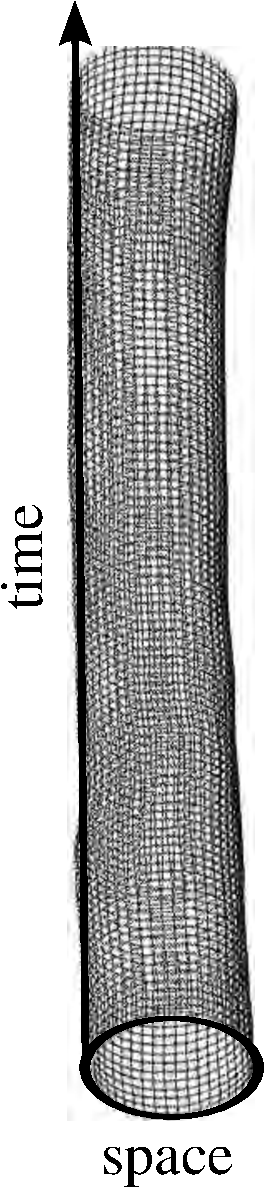
\includegraphics[width=.75\textwidth]{cylinderTime1}
    \vfill
\small{\texttt{(a)}}
\end{minipage}
~~~~
\begin{minipage}[height=.20\textheight]{.75\textwidth}
\centering
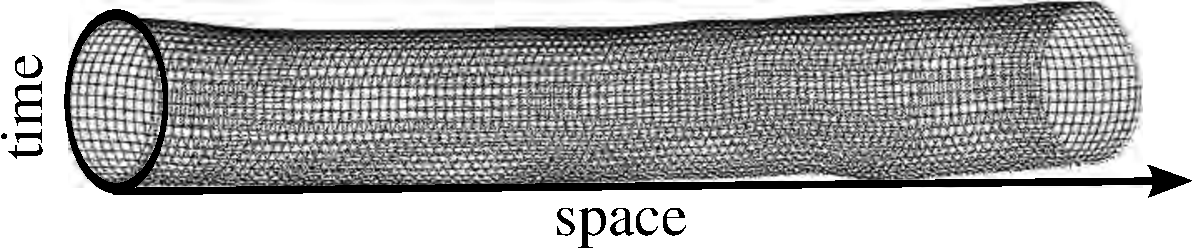
\includegraphics[width=.80\textwidth]{cylinderSpace1}
\\
\small{\texttt{(b)}}
\\
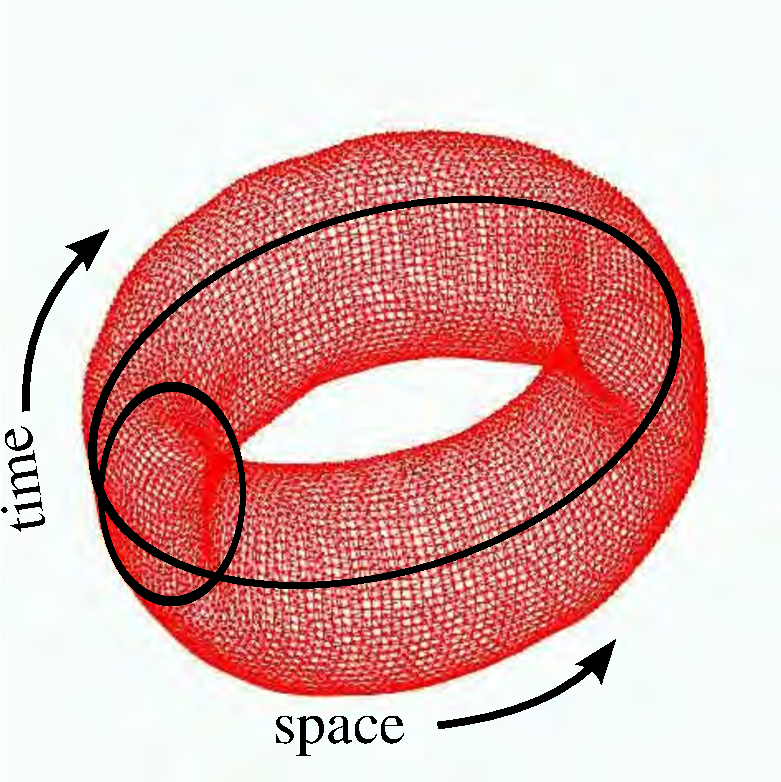
\includegraphics[width=.50\textwidth]{spaceTime1}
\\
\small{\texttt{(c)}}
\end{minipage}
    \end{center}
\caption{\label{fig:spaceTime1}
(a) The 1D \KSe\ is usually integrated on a \spt\ cylinder of an
    arbitrary fixed $\speriod{}$ periodic spatial extent, with time
    $\zeit\in\{-\infty,\infty)$; for an example, see \reffig{f:ks_largeL}.
(b) It is also possible to integrate the equation on a \spt\ cylinder of an
    arbitrary fixed $\period{}$ periodic temporal extent, with position
    ranging over $\conf\in\{-\infty,\infty)$, see \refsect{sect:KSspaceInt}.
(c) Here we shall seek {\spt}ly \twot\ solutions $u(\conf,\zeit)$ over a 2-torus of
    dynamically determined size $(\speriod{},\period{})$ , see
    \refsect{sect:KStwots}.
}
\end{figure}
%%%%%%%%%%%%%%%%%%%%%%%%%%%%%%%%%%%%%%%%%%%%%%%%%%%%%%


Smooth, spatially periodic velocity field $u$ %(\conf,\zeit)=u(x+\speriod{},\zeit)$
is naturally represented in the Fourier space,
\beq
  u(\conf,\zeit)
   =\sum_{m=-\infty}^{+\infty} a_m(\zeit)\,e^{ i 2\pi m\conf /\speriod{} }
\,,
\ee{eq:ksexp}
with the $1$D PDE \refeq{e-ksL}
replaced by an infinite set of
ODEs for the complex Fourier coefficients $a_m(t)$:
\beq
\dot{a}_m %= \pVeloc_m(a)
     = ( q_m^2 - q_m^4 )\, a_m
    - i \frac{q_m}{2} \sum_{k=-\infty}^{+\infty} a_k a_{m-k}
\ee{SCD07:expan}
where $q_m =  2\pi m/\speriod{}$.
Since $u(\conf,\zeit)$ is real, $a_m=a_{-mm}^\ast$, and we can replace the
sum by a $m > 0$ sum.


Consider the \KSe\ \refeq{e-ks} on a {\spt} cylinder
$(\conf,\zeit)\in([0,\speriod{}),\reals)$, defined on a a spatial strip of width
$\speriod{}$, with spatially periodic boundary condition $u(\conf,\zeit)=u(x+\speriod{},t)$, see
\reffig{fig:spaceTime1}\,(a).
Discretize spatially the \KS\ system by Fourier expanding the field
$u(\conf_n,\zeit)= u_n(\zeit)$ over $N$ points of a periodic spatial 1D
lattice $\conf_n=n\speriod{}/N$,
\bea
  \Fu_k(\zeit) &=& \frac{1}{N} \sum^{N-1}_0 u_n(\zeit) e^{-iq_k\conf_n}
  \,=\, \frac{1}{N} \sum^{N-1}_0 u_n(\zeit) e^{-i 2 \pi k n /N}
  \,,\quad
q_k = \frac{2 \pi k}{\speriod{}}
\continue
  u_n(\zeit) &=&\sum_{k=0}^{N-1}\Fu_k(\zeit) e^{iq_k\conf_n}
    \,=\, \sum_{k=0}^{N-1}\Fu_k(\zeit) e^{i 2 \pi k n /N}
\,,
\label{spatFT}
\eea
and expressing \refeq{e-ks} in terms of discrete spatial Fourier modes as
$N$ ordinary differential equations (ODEs) in time
\beq
%\dot{\Fu}_k(\zeit)
\frac{d~}{d\zeit}\Fu_k(\zeit)
= ( q_k^2 - q_k^4 )\, \Fu_k(\zeit)
- \frac{i q_k}{2} \!\sum_{k'=0}^{N-1} \!\!\Fu_{k'}(\zeit) \Fu_{k-k'}(\zeit)
\,.
\label{e-Fks}
\eeq

        \PCedit{
In the Fourier representation the \reqva\ time dependence is
\beq
 a_k(t) e^{-itc q_k} = a_k(0)
\,.
\ee{reqvaF}
Differentiating with respect to time, we obtain
the Fourier space version of the \reqv\ condition
\refeq{KSeqvCond},
\beq
 \pVeloc_k(a) - i q_k c a_k = 0
\,,
\ee{reqvCondF}
which we solve for (time independent) $a_k$ and $c$.
        }


%%%%%%%%%%%%%%%%%%%%%%%%%%%%%%%%%%%%%%%%%%%%%%%%%%%%%%%%%%%%%%%%%%
\subsubsection{Temporal stability}
\label{exam:KurSivTempstab}
% From ChaosBook Chapter{PDEs}{2016-01-23}{Turbulence?}

To calculate the temporal stability of a spatial \eqv\ $\Fu_\stagn$
    \PC{2019-05-16}{dropped
(or a temporally \po).
%\refeq{eq:StabMat} is plain wrong, no?
    }
we need to evaluate  the \stabmat\ (the matrix of temporal
velocity gradients)
\beq
%  \Mvar_{ij}(a_q)  = \left.\frac{\partial v_i}{\partial a_j}\right|_{a=a_q}
  \Mvar_{ij}(\Fu_\stagn)  =
  \left.\frac{\partial \dot{\Fu}_i}{\partial \Fu_j}\right|_{\Fu={\Fu_\stagn}}
\,.
\label{eq:StabMat}
\eeq
For \KS\ we can
compute $\Mvar(\Fu_q)$ efficiently using the linearity
of the Fourier transform, see \refref{SCD07}.
Consider the four matrices
$\frac{\partial \dot{b}_k}{\partial b_j},\frac{\partial
\dot{b}_k}{\partial c_j},\frac{\partial \dot{c}_k}{\partial
b_j},\frac{\partial \dot{c}_k}{\partial c_j}$,
where the real and imaginary parts of $\Fu_k$ are
$\Fu_k=b_k+ic_k$.
For illustration, consider the $b_k=0$ invariant antisymmetric subspace
$\bbU^+$,
\beq
\dot{c}_k= \pVeloc_k(c)
     = ( q_k^2 - q_k^4 )\, a_k
    - \frac{q_k}{2} \sum_{m=-\infty}^{\infty} c_m c_{k-m}
\,,\qquad   q_k = k/2\pi \speriod{}
\,.
\ee{expan}
The temporal {\stabmat} \refeq{eq:StabMat} restricted to the invariant
antisymmetric subspace $\bbU^+$ follows from \refeq{expan}:
\beq
{\Mvar}_{kj}(c) =\frac{\pde v_k(a)}{\pde c_j  }
=(q_k^2- q_k^4)\delta_{kj} + q_k ( c_{k-j}- c_{k+j})
\,.
\ee{expanMvar}
For the full \statesp, consult sect.~6.2 {\em Calculating stability of equilibria}
of Siminos thesis\rf{SiminosThesis}.

\subsubsection{\KS\ $u=0$ temporal equilibrium}
\label{sect:KSu0equiT}

The \KS\ flat flame front $u(\conf,\zeit)=0$ is always a temporal {\eqv} of \refeq{e-ks},
whose temporal {\stabmat} \refeq{expan} is
diagonal, with real temporal stability exponents $\eigExp[k]= q_k^2- q_k^4$,
the eigenvectors are spatial Fourier modes, and consequently the
temporal {\jacobianM} is diagonal as well,
\(
\jMps^t_{kj} = \delta_{kj} \ExpaEig_k(\zeit)
    \,,\;
\ExpaEig_k(\zeit) = e^{(q_k^2- q_k^4)\,t}
\,.
\)
%	} %end \example{\Stabmat,  antisymme
%%%%%%%%%%%%%%%%%%%%%%%%%%%%%%%%%%%%%%%%%%%%%%%%%%%%%%%%%%%%%%%%%%

% siminos/gudorf/thesis/chapter/KSspaceInt.tex
% $Author: predrag $ $Date: 2020-05-25 15:18:45 -0400 (Mon, 25 May 2020) $

%\subsection{Temporally periodic \KS}
%\label{sect:KSspaceInt}
%\hfill     2016-02-04 Burak

\MNGedit{

BLOG EXCERPTS

I would not use much time on improving integrators at this stage (the
flow is not Hamiltonian, but there is lots of literature on time-reversal
invariant dynamical systems - \refref{lamb98,LaWu02,Bosetti2010})

\begin{figure}[ht]
\begin{minipage}[height=.45\textheight]{.45\textwidth}
\centering \small{\texttt{(a)}}
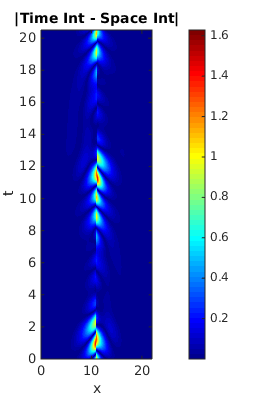
\includegraphics[width=\textwidth,height=.45\textheight]{MNGppo1m21e}
\end{minipage}
\begin{minipage}[height=.45\textheight]{.45\textwidth}
\centering \small{\texttt{(b)}}
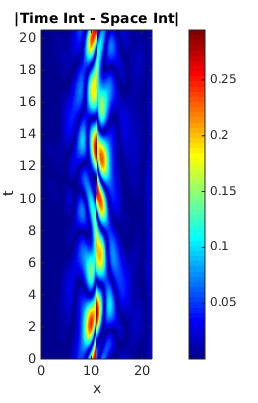
\includegraphics[width=\textwidth,height=.45\textheight]{MNGppo1m7e}
\end{minipage}
\caption{\label{fig:MNGppo1error}
Absolute error between time-integrated solutions of $\PPO{10.2}$ and spatially integrated solutions. A Time-periodic initial condition $T = [0,2\,T_{\PPO{10.2}})$ was taken from the time integrated solution. This initial time-strip was integrated spatially in two parts, $\conf = [0,11]$ and $\conf = [-11,0]$. The number of active Fourier modes in each plot are (a) 21, and (b) 7.
}
\end{figure}
}
Consider next the case of temporally periodic velocity field
\beq
    u(\conf, \zeit) = u(\conf, \zeit + \period{})
\label{e-PeriodicBC}
\eeq
on temporal domain of fixed period $\period{}$,
and any \conf, \ie, cylinder $(\conf,t) \in \reals \times [0,\period{})$, see
\reffig{fig:spaceTime1}\,(b).
%\KSe\ in one space dimension is
%\beq
%    u_\zeit =  - u u_\conf
%    -u_{\conf \conf}-u_{\conf \conf \conf \conf}\,,
%    \label{e-ks2}
%\eeq
%where subscripts denote partial derivatives.
In order to express
\KS\ as a set of first-order PDEs, define four fields
\beq
(u_{0},u_{1},u_{2},u_{3}) \equiv
(u,
u_{\conf},
u_{\conf \conf},
u_{\conf \conf \conf})
%    u_{0} \equiv u(\conf,\zeit) \,, \quad               % u^{(0)}
%    u_{1} \equiv u_{\conf}(\conf,\zeit) \,, \quad        % u^{(1)}
%    u_{2} \equiv u_{\conf \conf}(\conf,\zeit) \,, \quad  % u^{(2)}
%    u_{3} \equiv u_{\conf \conf \conf}(\conf,\zeit)      %  u^{(3)}
\,.
\eeq
Using the values of the four fields
%$(u_{0},u_{1},u_{2},u_{3})$
%$u( \conf_0, \zeit)$,
%$u_{\conf}( \conf_0, \zeit)$,
%$u_{\conf \conf}( \conf_0, \zeit)$,
%$u_{\conf \conf \conf}( \conf_0, \zeit)$,
for all $\zeit \in [0, \period{})$ at a fixed space point $\conf_0$,
as initial values,
one may attempt
to determine $u(\zeit, \conf)$ for any $\conf$ on a time-periodic strip
$\zeit \in [0, \period{})$ by solving the \KS\ \refeq{e-ks}
rewritten as a set of equations first order in spatial
derivatives
    \PC{2016-07-23}{The equations seem correct to me.
    The notation of \refrefs{LanThesis,lanCvit07} is different, but
    Burak's $u^{(j)}$ fields are easier to keep track of.
    {\bf 2019-05-18 PC} experimenting with $u_j$ format.
    }
\bea
    \frac{\partial}{\partial \conf} u_{0} &=& u_{1} \,,\quad
    \frac{\partial}{\partial \conf} u_{1} \,=\, u_{2} \,,\quad
    \frac{\partial}{\partial \conf} u_{2} \,=\, u_{3} \,, \label{e-ksX} \\
    \frac{\partial}{\partial \conf} u_{3} &=&
    - \frac{\partial}{\partial \zeit} u_{0} - u_{2} - u_{0} u_{1}
\nonumber
\,.
\eea
Given the time-periodic boundary condition \refeq{e-PeriodicBC},
it is natural to expand the \KS\ field $u(\conf,\zeit_n)= u_n(\conf)$ as a temporal Fourier
$u(\conf,\zeit_n)= u_n(\conf)$ over $M$ points of a periodic
temporal lattice $\zeit_n = n \period{}/M$, $n=0,1,\cdots,M-1$:
\beq
    u_{i}(\conf, \zeit) = \sum_{n = 0}^{M-1}
    \Fu_{i,n}(\conf)\,e^{i \omega_n \zeit_n} \, , \quad \mbox{where }
    \omega_n = 2 \pi n / \period{} \, .
\ee{BBtemporFourier}
Rewriting \refeq{e-ksX} in terms of temporal Fourier modes,
we obtain $4M$ ordinary differential equations,
\bea
\frac{\partial}{\partial \conf} \Fu_{0,n} &=& \Fu_{1,n}
         \continue
\frac{\partial}{\partial \conf} \Fu_{1,n} &=& \Fu_{2,n}
        \continue
\frac{\partial}{\partial \conf} \Fu_{2,n} &=& \Fu_{3,n}
        \label{e-FksX} \\
\frac{\partial}{\partial \conf} \Fu_{3,n}
      &=&
 - i \omega_n \Fu_{0,n} - \Fu_{2,n}
 - \sum_{n' = 0}^{M-1} \Fu_{0,n - n'} \Fu_{1,n'}
\,. \nonumber
\eea
%Due to their instabilities, these equations might
%be hard to integrate numerically.
    \PC{2016-09-12, 2016-09-23}{Checked, except for the range of $n'$.}

\subsubsection{Integrating \KS\ on a $\period{}=0$ line}
\label{sect:KSeqva}

    \PCedit{
[{\bf 2016-02-06 Predrag}
summarize the Michelson\rf{Mks86} case on the spatial $\speriod{}\to\pm\infty$ domain.
Review the reflection-invariant subspace discussed in
Lan's thesis\rf{LanThesis} and his thesis-work article\rf{lanCvit07,DoLa14}.
Then set up the full \On{2} equivariant case, and describe the
\On{2}-symmetry reduced case, following \refrefs{BudCvi14,BudCvi15}.
]
    }

%%%%%%%%%%%%%%%%%%%%%%%%%%%%%%%%%%%%%%%%%%%%%%%%%%%%%%%%%%%%%%%%
\begin{figure}[t]
\begin{center}
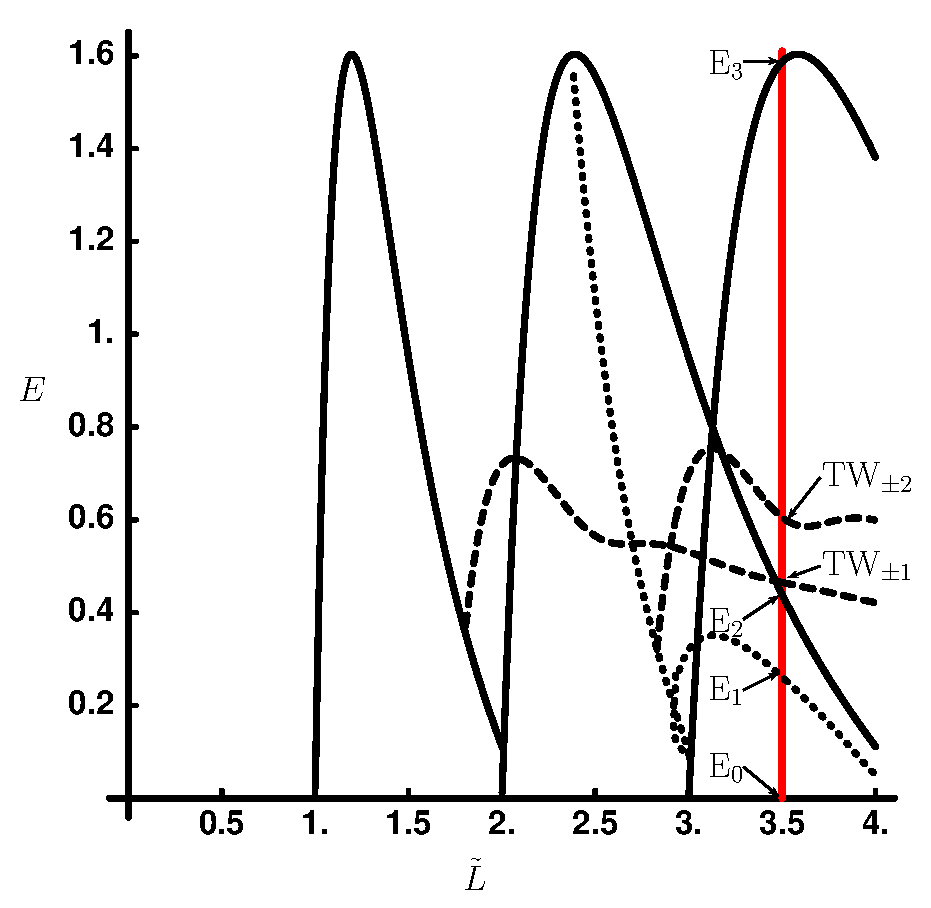
\includegraphics[width=0.5\textwidth]{ksBifDiag_pst}
\end{center}
\caption{\label{fig:SCD07ksBifDiag}
The energy \refeq{SCD07eq:stdks} %{ksEnergy}
of the \eqva\ and \reqva\ that
exist up to $\speriod{}=22$, $\tildeL = 3.5014\ldots$, plotted as a function
of the system size $\tildeL = \speriod{}/2\pi$ (additional \eqva, not present
at $\speriod{} = 22$ are given by Greene and Kim\rf{ksgreene88}). Solid curves denote
$n$-cell solutions \EQV{2} and \EQV{3}, dotted curves the GLMRT
\eqv\ \EQV{1},
and dashed curves the \reqva\ \REQV{\pm}{1} and \REQV{\pm}{2}.
The parameter $\alpha$ of \refrefs{KNSks90,ksgreene88} is
related to the system size by $\tildeL=\sqrt{\alpha/4}$.
(From Cvitanovi{\'c}, Davidchack and Siminos\rf{SCD07})
        }
\end{figure}
%%%%%%%%%%%%%%%%%%%%%%%%%%%%%%%%%%%%%%%%%%%%%%%%%%%%%%%%%%%%%%%%%%

%     BB 2016-02-04, PC 2016-09-23
If $u$ is a temporal \eqv, $u = u(\conf+v\zeit,0)$ whose spatial profile
does not change in time, with a vanishing $u_t=0$ (for an \eqv) or a constant
traveling wave velocity $u_t=v$ (for a \reqv), one can integrate \refeq{e-ks}
\beq
    u_\zeit -v = 0
    = - \left(u^2/2 -u_{\conf}-u_{\conf \conf \conf}\right)_{\conf}
\label{e-ksSteady}
\eeq
once over space, and the highest order derivative in \refeq{e-ksX}
becomes the third order\rf{Mks86,LanThesis,lanCvit07,DoLa14}. We shall
refer to this case as the $\period{}=0$ temporal strip, as specifying $u
= u(\conf_0,0)$ at $\zeit=0$ instant suffices to initialize the spatial
evolution, which in this case is given by a set of three ODEs and an
integration constant, which can be interpreted as the energy density $\expctE$,
\beq
\expctE = {\textstyle\frac{1}{2}}u^2 - c u + u_x + u_{xxx}
\,.
\label{SCD07eq:stdks}
\eeq
% \PCpost{2018-05-30}{
Computationally, it is more robust to compute $\expctE$ by averaging over $\speriod{}$,
as in \refeq{SCD07ksEnergy}.

Eqs.~\refeq{e-ksX}, however, remain a set of four PDEs for any
$\period{}>0$ temporal strip.

\subsubsection{Spatial stability of $u=0$ equilibrium}
\label{sect:KSu0equiS}

To calculate the spatial stability of a spatial \eqv, we need to evaluate
the \stabmat\ of the system in the complex representation \refeq{e-FksX}
in terms of the 16 sub-blocks
\beq
  \Mvar_{ij}^{IJ} (\Fu)  =
\frac{\partial \Fu^{'}{}^{(I)}_i}
     {\partial \Fu{}^{(J)}_j}
\,,\qquad
    \Fu^{'} = \Fu_x
\,.
\ee{eq:StabMatBlocks}
The trivial \eqv\ of \refeq{e-FksX} is given by $\Fu^{(I)}_{j}=0$.
In terms of $[M\!\times\!M]$ temporal Fourier modes blocks its spatial
\stabmat\ is
\beq
\Mvar^{IJ}(0) =
\begin{bmatrix}
  0 & 1 & 0 & 0 \\
  0 & 0 & 1 & 0 \\
  0 & 0 & 0 & 1 \\
\mbox{Diag}\{-i \omega_k\} & 0 & -1 & 0
\end{bmatrix}
\ee{PCeqvaStblty}
%Here
%\beq
%\begin{bmatrix}
%  0 & 1 & 0 & 0 \\
%  0 & 0 & 1 & 0 \\
%  0 & 0 & 0 & 1 \\
%Diag\{-i \omega_k\} & 0 & 0 & 0
%\end{bmatrix}
%\ee{PCcyclic}
%is cyclic of order 4 and thus has a nice characteristic equation, but the
%$\Mvar^{02} (\Fu) =-1$ screws that up.

% siminos/gudorf/thesis/chapter/KStwots.tex
% $Author: predrag $ $Date: 2020-05-25 15:18:45 -0400 (Mon, 25 May 2020) $

% called by
%           siminos/spatiotemp/chapter/spatiotemp.tex
%           siminos/tiles/GuBuCv17.tex

%\section{\KS\ on a torus}
%\label{sect:KStwots} % KSspacetime}

Here we propose to describe all solutions $u(\conf,\zeit)$ of \KSe\ \refeq{e-ks} as the
closure of the union of the set of all prime (non-repeating)
\twots\
\bea
u(\conf,\zeit) &=& u(\conf,t+\period{})
       \;=\; u(\conf+\speriod{},t)
\continue
       &=&  u(\conf+\speriod{},t+\period{})
\,,\quad
(\conf,\zeit)\in([0,\speriod{}),[0,\period{}))
\,.
    \label{e-ksTorus}
\eea

Consider a torus $(\speriod{},\period{})$ with {\spt}ly
doubly-periodic $u(\conf,\zeit)=u(x+\speriod{},t+\period{})$,
$(\conf,\zeit)\in([0,\speriod{}),[0,\period{}))$, see
\reffig{fig:spaceTime1}\,(c), and combine the discrete spatial
Fourier modes expansion \refeq{spatFT} with the discrete temporal Fourier
modes expansion \refeq{BBtemporFourier}.
Discretize $u(\conf_n,\zeit_m)= u_{nm}$ over
$N$ points of a periodic spatial lattice $\conf_n = n \speriod{}/N$,
and
$M$ points of a periodic temporal lattice $\zeit_m = m \period{}/M$,
%\beq
%    \Fu_{k,m}^{(i)} = \frac{1}{M} \sum_{n = 0}^{M-1}
%    \Fu^{(i)}_{k,n} e^{i \omega_n \zeit_m}
%    \, , \quad
%    \Fu^{(i)}_{k,n} = \sum_{m=0}^{M-1}\Fu_{k,m}^{(i)}  e^{-i \omega_n \zeit_m}
%    \, , \quad
%    \mbox{where }
%    \omega_n = 2 \pi n / \period{} \, .
%\eeq
%
\bea
\Fu_{kj} &=&
  \frac{1}{NM} \sum^{N-1}_{n=0} \sum^{M-1}_{m=0}
  u_{mn} \, e^{-i(\wavek \xm + \freqj \tn)}
    \,,\quad
\wavek = \frac{2 \pi k}{\speriod{}}
    \,,\;
\freqj = \frac{2 \pi j}{\period{}}
    \continue
u_{mn} &=&\sum_{k=0}^{M-1}\sum^{N-1}_{j=0}
   \Fu_{kj} \, e^{i(\wavek \xm + \freqj \tn)}
\,,
\label{spattempFT}
\eea
In its Fourier discretization, \KS\ PDE \refeq{e-Fks} is a set of $MN$
algebraic equations for the {\spt} Fourier coefficients $\Fu$,
\beq
\left[ i \freqj - ( \wavek^2 - \wavek^4 ) \right]\Fu_{kj}
+ i \frac{\wavek}{2} \!\sum_{k'=0}^{M-1} \sum^{M-1}_{j'=0}\!\!
\Fu_{k'j'} \Fu_{k-k',j-j'}
    = 0
\,.
\label{e-FksSpattemp}
\eeq
In other words, we have reduced the problem of either temporal or
spatial evolution on a
{\spt}ly periodic domain to the fixed point problem of determining an
invariant 2-torus, a fixed point in the $NM$\dmn\ \statesp.

\MNG{2019-05-13}{Elimination of space and time
translations effectively reduces the codimension of each solution by two, this is
undesirable when numerically solving the \refeq{e-pseudospectral} in a least-squares sense}
First, however, we must eliminate the temporal translation marginal eigenmode
by a {\PoincSec}, and the spatial translation marginal eigenmode by a {\slice}.
Generically, they both can fixed by the first Fourier mode {\PoincSec} /
{\slice}.
The Newton method then requires inversion of $1-J$, \ie,
$\det(1-J)$, where $J$ is the 2-torus \jacobianM.
    %
    \PC{2018-04-08}{see also \refsect{sect:KurSivSpTmpStab}.}

We can generalize the notion of average `energy' density
\refeq{SCD07ksEnergy} and apply it to any \twot\ $p$ by also
averaging over time
\beq
    \expctE_p=
  \frac{1}{\speriod{}\period{}}\!\oint d\pSpace\oint d\zeit \frac{u^2}{2}
  \,,
  \label{twotEnergy}
\eeq
The Fourier space average spatial energy density \refeq{SCD07EFourier}
generalized to any {\spt} solution \refeq{spattempFT} is then:
\beq
\expctE
          =  \sum_{k=0}^{N-1}\sum^{M-1}_{n=0}
             {\textstyle\frac{1}{2}}|\Fu_{kn}|^2
\,.
\ee{twotEFourier}


\subsection{Spatiotemporal $u=0$ equilibrium}
\label{sect:KSu0equiST}

    \PC{2019-03-16}{
    Incorporate here the spatial evolution stability analysis of
    blog posts starting with {\bf 2016-09-02 Matt Stability of u=0 equilibria}.
   }
   %
Consider the $\Fu_{kn}=0$ \eqv\ of \refeq{e-FksSpattemp}. Its
linearization is
    \MNG{2016-09-12 }{
\MNGedit{Added the factor of $i$ that was missing in \refeq{e-FksSpattemp}}
\PCedit{2016-09-23 restored signs to match \refeq{e-Fks} and \refeq{e-FksSpattemp}}
    }
\bea
i \omega_n  &=&  q_k^2 - q_k^4
    \continue
i \frac{2\pi n}{\period{}}   &=&
\left(\frac{2\pi k}{\speriod{}}\right)^2 - \left(\frac{2\pi k}{\speriod{}}\right)^4
\,.
\label{e-FksSpattemp0}
\eea
The two special cases are the spatial strip of \refsect{sect:KStimeInt},
which yields the $2N$ real temporal stability exponents
$\Lyap_k=i\omega(k)$ for a fixed spatial strip of width $\speriod{}$, and the
temporal strip of \refsect{sect:KSspaceInt}, which yields the $4+8(M-1)$ complex
spatial stability exponents $i q^{\pm,\pm}(n)$ for a fixed temporal strip of period
$\period{}$, as the four solutions of the quartic equation \refeq{e-FksSpattemp}
for each $i \omega_n$, $n = 0, \pm 1, \pm 2, \pm M/2$ :
\beq
(i q_k)^4 + (i q_k)^2 + i \omega_n  =0
    \quad\Rightarrow\quad
i q^{\pm,\pm}(n) = \pm \sqrt{(-1\pm \sqrt{1 -4 i \omega_n})/2}
\ee{spatialStabExp}
    \MNG{2016-09-20}{
    I think I should have been looking for $i q_k$ not $q_k$? If so, it
    matches the stability exponents of \refeq{PCeqvaStblty} %\refeq{MNGeqvaStblty}
    }
Each solution appears twice, corresponding to  $(\omega_n,-\omega_n)$,
except for
\beq
q^{\pm,\pm}(0) = \mp i\sqrt{(-1\pm 1)/2} =
(0,0,-1,1)
\,.
\ee{spatialStabExp0}
There are two root magnitudes for each $n \neq 0$, independent of the
sign of $n$:
%\[%beq
%|q^{\pm,\pm}(n)|^2 = (-1\pm \sqrt{1 +4 i \omega_n})
%(-1\pm \sqrt{1 -4 i \omega_n})/4
%\]%ee{spatialStabExp01}
%
\beq
|2q^{\pm,\pm}(n)|^2 = 1+ \sqrt{1 +  16 \omega_n^2}
\pm \sqrt{1 +4 i \omega_n}
\pm \sqrt{1 -4 i \omega_n}
\,.
\ee{spatialStabExp1}

\subsection{Spatiotemporal stability}
\label{sect:KurSivSpTmpStab}

Let
$u_\stagn(\conf,\zeit)$ be a doubly-periodic solution of \refeq{e-FksSpattemp} on the
$(\conf,\zeit)\in[0,\speriod{})\times[0,\period{})$ torus, a point in the
$\speriod{}\,\period{}$\dmn\ \statesp. Add an arbitrary small perturbation field
$\delta u(\conf,\zeit)$, also doubly periodic. Linearize \refeq{e-FksSpattemp}.
The linearized operator acting on $\delta u(\conf,\zeit)$ must annihilate it, \ie,
(WRONG AS IT STANDS)
\[
(J(u_\stagn) -\ExpaEig_j \matId)\delta u =0
\]
where the \jacobianM\ is the linearization over the whole 2-torus
\beq
J(\Fu_\stagn)_{kn} =
\left[ i \omega_n - ( q_k^2 - q_k^4 ) \right]\delta_{kn}
+ i q_k\!\sum_{k'=0}^{N-1} \sum^{M-1}_{m'=0}\!\!
\Fu_{k'm'} \delta_{k-k',m-m'}
\,.
\label{e-FksSpTmpJac}
\eeq
In $d=1$ case (pure temporal evolution) $\det(J(u_\stagn) -\matId)$ is the
usual period $\period{}$ cycle weight, this time obtained not by integration in
time but by evaluating the determinant of the Toeplitz matrix over the whole
cycle in one go (this might be familiar to some from the path-integral
derivation of Gutzwiller formula cycle weight. With \refeq{e-FksSpTmpJac},
$\det(J(u_\stagn) -\matId)$ is the pattern weight in $d=2$, and this
generates to defining the invariant weight for any $d$-torus.
 

%%%%%%%%%%%%%%%%
% Chapter 2
%%%%%%%%%%%%%%%%
\chapter{Spatiotemporal Formulation}
\label{c-formulation}
%\section{Motivation}
%In light of all of these difficulties we believe that new, bold ideas are
required to resume forward progress. Specifically, we have begun a completely
{\spt} formulation of chaos which treats all continuous dimensions democratically.
The main idea is to discard the idea of a dynamical system completely; exponential
instabilities mean that conventional methods never could have worked. By converting to
a truly {\spt} formulation we have discarded dynamics and the inherent difficulties therein.
This allows us to quantify and characterize infinite space-time via shadowing
of fundamental {\spt} patterns.

The primary claim that we make is that in hindsight, describing turbulence
via an exponentially unstable dynamical equation never could have worked.
Conventional methods treat spatial dimensions
as finite and fixed and time as inherently infinite.
Our {\spt} formulation of chaos treats all continuous dimensions with translational
invariance democratically as $(1+D)$ different `times'.
The proposal is inspired by the Gutkin and Osipov\rf{GutOsi15}
modelling of chain of $N$ coupled particle by temporal evolution of a
lattice of $N$ coupled cat maps.

The alternative that we propose to describe infinite space-time chaos via
the shadowing of fundamental patterns which we refer to as ``tiles''.
These tiles are the minimal ``building blocks'' of turbulence; they are realized
as \twots\ which are global solutions with compact support.
Finding the tiles of turbulence is fundamentally easier than finding
\twots\ on larger domains due to the exponential growth in complexity of
solutions. In other words there are fewer important solutions on smaller
domains. This in turn implies that there can only be a small
number of fundamental tiles. This is what makes the problem tractable:
if we can collect the complete set of tiles then we have the ability to
construct every \twot\ according to our theory.

The lack of exponentially unstable dynamics has powerful and immediate effects.
Because there is no time integration, the problem of finding \twots\ is
now a variational one. The benefit of this is that there is no need to start
an initial guess on the attractor; the optimization process handles this
entirely. This allows us to find arbitrarily sized \twots but in fact
there is no need to. Our hypothesis is that we need only to find the
building blocks which shadow larger \twots\ and infinite space-time.

The {\spt} formulation allows a much easier categorization of what is
``fundamental'' by virtue of the frequency that patterns admit in the
collection of \twots. By identifying the most frequent patterns, we shall
clip these patterns out of the \twots\ they shadow and use them as initial
conditions to search for our tiles.

The notion of ``building blocks of turbulence'' is one of the reasons for
studying fluid flows in the first place. There is evidence that certain
physical processes are fundamental, but they have yet to be used in a
constructive manner. The {\spt} description is able to actually put
these ideas in practice.
The \spt\ completely avoids this by constructing larger \twots\
from the combination of smaller \twots.
The reason
why the search for the fundamental tiles is classified as ``easy'' is because
in the small domain size limit there just aren't that many \twots; the dynamics
is relatively simple.

The first key difference is that the governing equation
dictates the \spt\ domain size in an unsupervised
fashion. The results here are not
The only reason why $L$ was treated as fixed is due to the
inherent instability it includes when treated as a varying quantity.
This small detail, allowing the domain size $L$ to vary,
is not as trivial as it seems.
 This difficulty
is especially evident in the \KSe, whose spatial derivative terms
are of higher order than the first order time derivative, but also
there is a spatial derivative present in the nonlinear component.

Specifically, we propose to study the evolution of \KS\ on the $2$\dmn\
infinite {\spt}domain and develop a $2$\dmn\ symbolic dynamics for it:
the columns coding admissible time itineraries, and rows coding the
admissible spatial profiles. Our {\spt} method is the clear winner in
both a computational and theoretical sense. By converting to a tile based
shadowing description we have essentially removed the confounding notion
of an infinite number of infinitely complex {\twots} from the discussion.
Now we must put these ideas into practice.

The testing grounds for these ideas will be the \spt\ \KSe

\beq \label{e-ks}
u_t + u_{xx} + u_{xxxx} + u u_x = 0 \quad \mbox{where} \quad x\in[0,\speriod{}], t\in[0,\period{}]
\eeq
where $u = u(x, t)$ represents a \spt\ velocity field. This
equation has been used to model many different processes such as
the laminar flame front velocity of Bunsen burners.
While \refeq{e-ks} is much simpler than the {\spt} Navier-Stokes equation,
we would argue that the main benefit is the simplicity of
visualizing its two-dimensional space-time. This visualization
makes the arguments more understandable and compelling in addition
to making the tiles easier to identify.

The plans for our {\spt} formulation have been laid bare. The main concept is that the infinities
of turbulence can be described by {\spt} symbolic dynamics whose letters are fundamental {\spt}
patterns. Consequentially, we have created numerical methods which not only perform better than
conventional methods but also present incredible newfound capabilities. These newfound capabilities
include but are not limited to finding small \twots\ which shadow larger \twots\ but also constructing
larger \twots\ from smaller ones. These new and robust methods alone present a way forward for turbulence research, hence their is merit in a {\spt} formulation even though the theory has not
been fully fleshed out.

To test our \spt\ ideas we require three separate numerical methods: the first
should be able to find \twots\ of arbitrary domain size. The second needs to be able to
clip or extract tiles from these \twots. Lastly, we need a method of
gluing these tiles together. All three of these techniques require the ability
to solve the optimization problem $F(\Fu,\speriod{},\period{})=0$
on an arbitrarily sized doubly periodic domain.

The primary claim that we make is that in hindsight, describing turbulence
via an exponentially unstable dynamical equation never could have worked.
Conventional methods treat spatial dimensions
as finite and fixed and time as inherently infinite.
Our {\spt} formulation of chaos treats all continuous dimensions with translational
invariance democratically as $(1+D)$ different `times'.
The proposal is inspired by the Gutkin and Osipov\rf{GutOsi15}
modelling of chain of $N$ coupled particle by temporal evolution of a
lattice of $N$ coupled cat maps.

%\subsubsection{characterize and quantify all patterns}
The alternative that we propose to describe infinite space-time chaos via
the shadowing of fundamental patterns which we refer to as ``tiles''.
These tiles are the minimal ``building blocks'' of turbulence; they are realized
as \twots\ which are global solutions with compact support.
Finding the tiles of turbulence is fundamentally easier than finding
\twots\ on larger domains due to the exponential growth in complexity of
solutions. In other words there are fewer important solutions on smaller
domains. This in turn implies that there can only be a small
number of fundamental tiles. This is what makes the problem tractable:
if we can collect the complete set of tiles then we have the ability to
construct every \twot\ according to our theory.

%\subsubsection{no instabilities}
The lack of exponentially unstable dynamics has powerful and immediate effects.
Because there is no time integration, the problem of finding \twots\ is
now a variational one. The benefit of this is that there is no need to start
an initial guess on the attractor; the optimization process handles this
entirely. This allows us to find arbitrarily sized \twots but in fact
there is no need to. Our hypothesis is that we need only to find the
building blocks which shadow larger \twots\ and infinite space-time.

%\subsubsection{Large to small}
The {\spt} formulation allows a much easier categorization of what is
``fundamental'' by virtue of the frequency that patterns admit in the
collection of \twots. By identifying the most frequent patterns, we shall
clip these patterns out of the \twots\ they shadow and use them as initial
conditions to search for our tiles.
%\subsubsection{small to large}
The notion of ``building blocks of turbulence'' is one of the reasons for
studying fluid flows in the first place. There is evidence that certain
physical processes are fundamental, but they have yet to be used in a
constructive manner. The {\spt} description is able to actually put
these ideas in practice.
The \spt\ completely avoids this by constructing larger \twots\
from the combination of smaller \twots.
The reason
why the search for the fundamental tiles is classified as ``easy'' is because
in the small domain size limit there just aren't that many \twots; the dynamics
is relatively simple.

%\subsubsection{numerical benefits?}
The first key difference is that the governing equation
dictates the \spt\ domain size in an unsupervised
fashion. The results here are not
The only reason why $L$ was treated as fixed is due to the
inherent instability it includes when treated as a varying quantity.
This small detail, allowing the domain size $L$ to vary,
is not as trivial as it seems.
 This difficulty
is especially evident in the \KSe, whose spatial derivative terms
are of higher order than the first order time derivative, but also
there is a spatial derivative present in the nonlinear component.



Once the collection is deemed sufficient we proceed to visual inspection. In this manner
we determine the most frequent patterns and single them out as tile candidates. This is
done by literally clipping them out of the \twots\ that they shadow. Each clipping is
then treated as an initial guess for a fundamental tile which is itself a \twot. Therefore,
these represent initial conditions for the optimization method. It is not a guarantee
that every clipping converges to a \twot; therefore the number of attempts to find a tile
should continue until it does in fact converge. The number of convergence attempts is typically
proportional to how confident we are that the pattern being scrutinized is in fact a tile.

Once a collection of tiles is collected, we can construct new and reproduce known \twots.
This is completed with a method we refer to as ``gluing''. It is as straightforward as one
might infer: tiles are combined in a {\spt} array to form initial conditions used to find larger
\twots. Methods of gluing temporal sequences of \twots\ exist but never has the ability to
glue \twots\ spatiotemporally existed before.

With the implementation of the gluing method can begin to
probe the 2\dmn\ {\spt} symbolic dynamics
previously mentioned. A fully determined symbolic dynamics is sufficient
to describe infinite space-time completely.
We already have the two edges of this symbol plane - the $\speriod{}=22$ minimal
cell\rf{SCD07,lanCvit07} is sufficiently small that we can think of it as
a low-dimensional (``few-body'' in Gutkin and Klaus
Richter\rf{EPUR14,EDASRU14,EnUrRi15,EDUR15} condensed matter parlance)
dynamical system, the left-most column in the Gutkin and
Osipov\rf{GutOsi15} $2D$ symbolic dynamics {\spt} table (not a
1\dmn\ symbol sequence block), a column whose temporal symbolic dynamics
we will know, sooner or later. Michelson\rf{Mks86} has described the
bottom row. The remainder of the theory will be developed from the
bottom up, starting with small {\spt} blocks.



Therefore we offer a new {\spt} formulation of chaos which
treats all dimensions with continuous symmetries democratically as $(D+1)$ different `times'.
This equal treatment of space and time removes the requirement for
spatial dimensions to be finite or fixed. In other words,
the role of spatial periods is now identical to that of time periods
in the sense that they are
variables determined by the governing equations.
    \PCedit{ % 2020-05-07
`Tiling' in the title of this paper refers to our attempt to
systematically triangulate this set in terms of dynamically invariant
solutions (\eqva, \po s, $\ldots$), in a PDE representation and numerical
simulation algorithm independent way.
    }

Within this framework there
are no longer any dynamics; instead, solutions are {\spt} combinations of
$(D+1)$ invariant tori (to which we shall henceforth refer to simply as \emph{{\po}s}).

While there are an infinite number of {\po}s our theory only utilizes a small
number of very important ones. We denote these special orbits as {\fpo}s and claim
that they are the long sought after ``building blocks''
of turbulence; that is, every solution can be described as a collection of {\fpo}s.

The goal is to collect, enumerate and utilize all {\fpo}s.
The collection of {\fpo}s proceeds in the following manner:
identify the most frequently recurring patterns in a collection of {\po}s,
extract and use said patterns as initial guesses for {\fpo}s. Taking the
unique results from this search establishes a finite collection or library
of {\fpo}s.
All {\po}s can then be constructed from a complete collection of {\fpo}s; we
aim at least collecting the most important {\fpo}s for now.

%\section{theory}
%\begin{description}
\item[KSe N-S comparison]
As previously stated, the testing grounds for these ideas will be the \spt\ \KSe
% Are we relabeling all equations?
\beq \label{e-ks}
u_t + u_{xx} + u_{xxxx} + u u_x = 0 \quad \mbox{where} \quad x \in [0,L], t\in [0,T]
\eeq
where $u = u(x, t)$ represents a \spt\ velocity field. This
equation has been used to model many different processes such as
the laminar flame front velocity of Bunsen burners.
This was chosen as the testing ground for our ideas because it has
a two dimensional space-time and has many similarities to the Navier-Stokes
equations. It is useful to relate the terms between the two equations via
the physical processes that they represent even though these processes aren't
The numerical challenge is to find
discretized velocity fields $u(x, t) \approx u(x_m, t_n)$
which satisfy the \KSe\ locally at every lattice site.

\item[2-tori, translational invariance, Fourier]
% Reformulate using Fourier modes
The translational invariance and periodicity make
\spt\ Fourier modes the natural representation of our equations.
The inherently infinitely dimensional equations are approximated
by a Galerkin truncation of the \spt\ Fourier modes.
The velocity field $u(x_m, t_n)$ with $x_m = \frac{mL}{M}$ and $t_n = \frac{nT}{N}$
can be described by a set of \spt\ \Fcs, represented as a vector $\Fu$. The indices
which indicate the \spt\ frequencies each mode represents are withheld as computational
details that would only bog us down at this stage of the discussion.
The \KSe\ \refeq{e-ks} in terms of the \Fcs\ $\Fu$ is a
system of differential algebraic equations
$\Fu$
\bea \label{e-kssFb}
%KSe in Fourier basis, pseudo-spectral form.
F(\Fu, L, T) &\equiv& (\omegaj - \wavek^2 + \wavek^4) \Fu + \frac{\wavek}{2} \FFT(\IFFT(\Fu)^2)\,.
\eea
The nonlinear term is computed in a \emph{pseudospectral} fashion: a method which computes the
nonlinear term as a product in physical space as opposed to a convolution in spectral space.
The definitions of each term is as follows; $\FFT$ and $\IFFT$ represent the forward and backwards
\spt\ Fourier transform operators. Spatial and temporal derivatives are calculated (most efficiently)
by element-wise multiplication with the appropriate power of the appropriate frequency vector.
Differentiation can be alternatively viewed as the ``lattice-wise'' multiplication of
the Fourier modes and a lattice of frequencies (this is sometimes referred to as the Hadamard product
or Schur product).

\item[Optimization problem]

\item[find library]
\item[large to small]
\item[small to large]
\end{description}
% Intro to the new possibilities/capabilities.
This attempt to overthrow the status quo includes multiple techniques
and methods that have not yet been witnessed in the literature.
The novelty of these methods result in newfound capabilities, which in turn allow for
new analyses. The utility and important properties of these methods
will be detailed later but we provide a preview here.

In this formulation we describe turbulence not as a series of temporal
snapshots but rather as a collection of {\spt} patterns. This formulation
is unconventional but appeals to our intuition; an example of {\spt} patterns
would be weather phenomena from the benign clouds to deadly hurricanes. Although
they technically represent movies, we treat space and time as equally as possible
by referring to these objects as {\spt} \emph{patterns}.
The claim is that when the laws of motion
have several commuting continuous symmetries (time-translation
invariance; space-translation invariance), all continuous symmetries
directions should be treated democratically, as $(1+D)$ different
`times'. The proposal is inspired by the Gutkin and Osipov \rf{GutOsi15}
modelling of chain of $N$ coupled particle by temporal evolution of a
lattice of $N$ coupled cat maps.
Specifically, we propose to study the evolution of \KS\ on the $2$\dmn\ infinite
{\spt}domain and develop a $2$\dmn\ symbolic dynamics for it: the
columns coding admissible time itineraries, and rows coding the
admissible spatial profiles.
We already have the two edges of this symbol plane - the $\speriod{}=22$ minimal
cell\rf{SCD07,lanCvit07} is sufficiently small that we can think of it as
a low-dimensional (``few-body'' in Gutkin and Klaus
Richter\rf{EPUR14,EDASRU14,EnUrRi15,EDUR15} condensed matter parlance)
dynamical system, the left-most column in the Gutkin and
Osipov\rf{GutOsi15} $2D$ symbolic dynamics {\spt} table (not a
1\dmn\ symbol sequence block), a column whose temporal symbolic dynamics
we will know, sooner or later. Michelson\rf{Mks86} has described the
bottom row. The remainder of the theory will be developed from the
bottom up, starting with small {\spt} blocks.


% Collection of twots
The first step required to construct our \spt\ theory
is to collect a library of \twots.
There are infinitely many such solutions but our search does not
need to be exhaustive, it only has to provide an adequate sampling
of the solution space. The notion of ``adequate'' is an inexact one,
broadly speaking, it consists of collecting \twots\ of various size and symmetry
types until all unique patterns have been accounted for.
Using this library the fundamental patterns will be determined by their
frequency in the library. It is possible to miss a specific pattern but this
is an indication that it is not fundamental and in all likelihood does not
account for any substantial porti An example of this
would be an isolated \twot in state space. It may have unique properties but
it doesn't get shadowed frequently enough to influence the infinite space-time
behavior.  The search ranges over all types of symmetries; the shadowing events within
the symmetric solutions are not symmetric themselves hence they may represent
fundamental tiles. This is important especially for {\rpo}s as they may contain tiles
whose local spatial drift is non-zero.


% Collection of tiles
By definition shadowing is not the exact realization of a \twot; it is a ``fuzzy window'' which
represents a local region of space-time that is in the proximity of
the \twot\ in question (in some norm). As the size of the shadowed \twot\
increases, so does the accuracy of the shadowing region. that is, away from
the boundary, the shadowing becomes exponentially more accurate.

Once a satisfactory library has been created, the search for tiles can begin. Visual
inspection of the library of \twots\ (enabled by the ease of visualization) helps
develop an intuition as to which patterns represent fundamental tiles.
 The tiles by our definition are subdomains which shadow large
\twots. It should be intuitive, therefore, to search for these tiles by numerically
``clipping'' them out of the larger \twots. This amounts to extracting sub-lattices from
the larger \twot\. This process is straightforward and intuitive; at least in the context
of a numerical method that can converge initial conditions that are periodic
in neither space nor time. These clippings are clearly
not \twots\ so they need to be run through the same numerical methods that were used
to converge the original \twot\ from which they originated. A successful outcome is not
guaranteed; this is likely a numerical property and not indicative of the importance of
the tile. The number of attempts to converge a tile should be proportional to
its frequency in our library. If a suspected tile repeatedly fails to converge then
either it is not a tile or it is not a minimal tile but a component of one; this latter
hypothesis would be evidenced by common occurrence of the suspected tile with another pattern.



% Gluing of fundamental solutions, tiles.
The next portion of the overarching \spt\ method assumes that not only a
large number of \twots\ have been found but also a handful of tiles.
The idea is to use these solutions as \spt\ building blocks in order to find new
solutions. Going even further, the eventual goal is to create a \spt\ symbolic dynamics
wherein the tiles are the alphabet. If this can be done then all solutions
are theoretically enumerable by \spt\ symbol blocks. This symbolic dynamics
has not been constructed as of yet but it is worth mentioning as it
serves as the overarching motivation.
This method of ``gluing'' solutions by combining them in space-time
presents not only a very attractive method for describing
\twots\ through fundamental physical behaviors but also for constructing
initial conditions to find arbitrary \twots.
This method in theory constitutes an improvement over both the dynamical systems formulation
as well as our own search using ``random'' initial conditions. This improvement
results from the ability to produce better initial conditions for our \spt\ searches.
The proof of concept for this method was the reproduction of a known
solution by gluing together tiles.

% What the tiles are going to be used for.
After the detailing and application of these methods we will have a
collection of fundamental tile solutions. With these tiles we layout out
case that infinite space-time can be described by these tiles. In addition,
we set the stage for how the investigation can process in a systematic manner.

The formulation of the \spt\ theory is dependent upon three main numerical processes;
finding \twots\ of arbitrary domain size, cutting out tiles from these \twots,
and gluing the tiles together. The first of these procedures requires the solving
of the optimization problem

There are many ways to solve this type of problem but before
we can begin solving the equation we need a method of generating
initial conditions.
As previously discussed, this work does not use
approximate recurrences; or time integration at all,
to generate initial conditions. Instead we simply
initialize a lattice of Fourier modes by first deciding
on the dimensions of the lattice and then assigning random %should I say reciprocal lattice? or not use lattice at all?
values to the modes. Random values in this case are
drawn from a normal distribution. The Fourier spectrum
is then rescaled to better represent the physical scales of the \KSe
and typical field magnitude of \twots. This modulation of
the spectrum is determined by two factors: the smoothness of
\spt\ solutions and the linear stability profile of
the \KSe. The smoothness or differentiability combined
with the bounded magnitude of the field implies that
the Fourier coefficients should decrease exponentially in
the in the infinite mode limit. Our heuristic
approach is not identical for space and time, so
we describe the process in detail. The rescaling
with respect to the spatial index linear stability profile of
the original dynamical equation is used as a rough
guide for the magnitude of the Fourier coefficients; the
easiest implementation is to just truncate the \spt\
modes at the boundary between linearly unstable
and linearly stable modes with respect to the
spatial index. For time, the strategy is the truncation of
nearly all of the modes. There is a time scale associated with
the problem, the Lyapunov time, but this simple strategy avoids the
calculation of this time. The intuition behind this choice is
that the general solution is comprised of many meandering "streaks";
shadowing of a one wavelength (in terms of physical scale) \eqv.
The truncation attempts to account for this approximately time independent
behavior in the locality of these streaks.

There are many different ways to approach this problem; we focus
on two different methods whose combination comprises
a robust numerical method.
The first
method substitutes an equivalent optimization problem
instead of directly solving $F=0$. The optimization
problem is formed by the construction
of a scalar cost function. Because we are concerned with
finding exact solutions to \refeq{e-kssFb} we elect
to simply use the $L_2$ norm of \refeq{e-kssFb} (with
a constant factor for convenience)
\beq
\mathcal{I}(\Fu, T, L) = \frac{1}{2}||F(\Fu, T, L)||_2^2 \,.
\eeq
There is no motivation for the specific choice of norm
or cost function other than they are simple choices which
satisfy our needs. The gradient of this cost function with
respect to a fictitious time, $\tau$, results in the fictitious
flow
\bea \label{e-descent}
\frac{\partial \mathcal{I}}{\partial \tau} &=& \nabla
\Big(\frac{1}{2}||F(\Fu, T, L)||_2^2\Big) \partial_{\tau}[\Fu, T, L] \continue
&=&
\Bigg(\Big[\frac{\partial F}{\partial \Fu}, \frac{\partial F}{\partial T},
\frac{\partial F}{\partial L} \Big]^{\top} F(\Fu, T, L)\Bigg) \cdot \partial_{\tau}[\Fu, T, L] \continue
&\equiv& \Big(J^{\top}F\Big) \cdot \partial_{\tau}[\Fu, T, L] \quad .
\eea
This equation \refeq{e-descent} by itself does not provide us with a descent direction
because the partial derivative of the independent variables with respect to $\tau$, $\partial_{\tau}[\Fu, T, L]$
remains undefined. Luckily, we are free to choose what it is. The only requirement
is a monotonically decreasing cost function. In other words, $\partial_{\tau}[\Fu, T, L]$
needs to be chosen such that $\frac{\partial \mathcal{I}}{\partial \tau}$ is
never positive. The most obvious choice is the
negative gradient of the cost function; this choice
corresponds to the gradient descent algorithm.
This is the most basic descent method, but it works very well when preconditioning is also included.
The details regarding the preconditioning are left out for brevity; it's a rough approximation to the
inverse of the linear portion of the equation. Regarding this choice of numerical method: originally,
we believed that our implementation represented a more sophisticated numerical method called the
\textit{adjoint descent algorithm} \rf{Faraz15}. Technically, the algorithm \emph{is} the adjoint
descent method, its just that with a lack of dynamics
the adjoint descent method collapses onto the gradient descent method. This fact wasn't realized
until much later but it worked so no harm no foul. If anything, this shows how much room there is
for numerical improvements. In any case, the choice that was made for the descent direction was
\beq
\partial_{\tau}[\Fu, T, L] = - \Big(J^{\top}F\Big) \,,
\eeq
such that
\beq
\frac{\partial \mathcal{I}}{\partial \tau} = -\Big|\Big| \Big(J^{\top}F\Big)\Big|\Big|_2^2 \leq 0 \,.
\eeq
It is clearly never positive but it can be equal to zero; this occurs at roots of $F$ but also local
extrema of $F$. The former is of course the desired state; the latter presents the problem of getting
stuck at local minima. Getting stuck at local minima is a very common problem in the field of optimization.
Instead of trying to eliminate this possibility we elect to merely account for this by termination of
the computation after a threshold is met. The actual
optimization process takes the form of numerical integration of the fictitious flow.
Numerical integration is of course affected by the integration scheme used. Luckily, we do
not care about the accuracy of the intermediate states as they are still approximations
and not exact solutions. The only true requirement is that the cost function must
monotonically decrease. Therefore we elected to use the simplest integration scheme: Euler's method.
Because this is first order and explicit, the accuracy depends on the step size. The step size
was determined by finding the first value of $\Delta x = 2^{-n}, n = 0, 1, \dots$ which reduced
the cost function. To again save time, this calculation was only performed once. Finding the optimal
distance to step using a line-search algorithm, for instance, drastically slows the
calculation. Another possibility would be to adapt the step size not at every step, but
at a finite number of checkpoints during the descent. These attempts always returned the
original step size such that these efforts are no longer attempted. If, at any point,
the numerical integration no longer decreases the cost function, then the step size
would be further reduced. The descent process was terminated whenever the step
size was reduced beyond a minimum value of $10^{-13}$. It could be argued that this threshold
should be changed to a larger value. Experientially it doesn't seem to affect the
calculation; further reduction of the step size almost always resulted in termination
of the descent. To increase the efficacy of our descent method, we also employed the
notion of preconditioning. The reason why we felt that preconditioning was warranted
was due to the stiff spatial derivative terms. The descent direction is dominated by
the components with high spatial frequencies but the magnitude of the corresponding
\Fcs\ are typically small. This can be counteracted by scaling the descent direction
such that the lower frequency modes are favored. The exact choice of preconditioner
is the inverse of the linear spatial derivative operators. This comes very cheap
as these operators are diagonal and is very effective for its price. Technically,
an absolute value is individually applied as to avoid division by zero. It is
also very beneficial to rescale the partial derivatives with respect to the
\spt\ domain parameters. The specific reason results from how poorly the
initial conditions approximate \twots. If nothing is done to control the
magnitude of these gradients, a very common occurence is that the solutions
are stretched out to incredibly large domains and either do not converge
or converge only to \eqva. These large \eqva, while perhaps desirable in
some circumstances, are not desired for our purposes as they are far
too unstable to be witnessed in infinite space-time.
The decision of when to cut off the gradient descent can
be determined in a variety of ways, the most common involve either the
absolute tolerance (magnitude of the cost function) or the relative tolerance
(change in cost function magnitude between steps).
We elect to use a combination of step limit and absolute tolerance. If the
cost function doesn't cross the threshold by the step limit then the descent is terminated.
Again these are some of the simplest conditions that ensure that the descent
will end in a reasonable amount of time.
The reason why this is acceptable is because the majority
of the heavy lifting is done by the back-end algorithm, the least-squares solver with backtracking.
In this context, the descent algorithm can be viewed as bringing approximate solutions
close enough to \twots\ such that the least-squares algorithm can converge them, akin
to \rf{Faraz15}



The second portion of our hybrid numerical method is
to apply a least-squares solver to the root finding problem $F=0$. The first step is everyone's
favorite derivation, the derivation of Newton's equations from the linearization about a root of $F$
\beq
F(\Fu+\delta\Fu, T+\delta T, L+\delta L)\approx
F(\Fu, T, L) + J \cdot [\delta\Fu, \delta T, \delta L] + \dots \,.
\eeq
substitution of zero for the LHS (the root) yields
\beq \label{newton}
J \cdot [\delta\Fu, \delta T, \delta L] = -F(\Fu, T, L) \,.
\eeq
where
\beq
J \equiv \Big[\frac{\partial F}{\partial \Fu}, \frac{\partial F}{\partial T}, \frac{\partial F}{\partial L} \Big] \,.
\eeq
This equation is of the general form for a linear system $Ax = b$; it is convenient to refer the system of
equations in this form. Technically, this equation is solved a number of times, each time producing its own
least-squares solution which guides the field to \twot. We avoid this here just to keep the notation clean.
It is implicit in the definition of $J$ that this is a rectangular linear system; there are more columns in
$J$ than rows. The equations are augmented to include variations in $T,L$ and there are no components of the
\KSe\ associated with this. Two choices for how the handle this are: create and include additional constraints
on either the \Fcs\ or the \spt\ parameters, or solve the equations in a least-squares sense.
We chose to solve the equations in a least-squares manner. We are not focused on finding specific
solutions so we can get away with this. Another reason is that a common choice for the constraints
is to fix the translational degrees of freedom, that is, ensure that the solutions to the linear system
\refeq{newton} are orthogonal to the partial derivatives $\frac{\partial \Fu}{\partial x}$ and
$\frac{\partial \Fu}{\partial t}$. These constraints are suboptimal for two reasons: they specify a particular
member of a group orbit beforehand reducing the likelihood to converge and the orthogonality to the direction of
spatial translations is not well defined for \twots\ with discrete symmetry. As briefly mentioned, we also
include the notion of backtracking; that is, the least-squares step is repeatedly divided by a factor of
two until either the cost function decreases or the step size becomes too small. This saves time in comparison to
line searching methods which find the optimal step size which produces the largest reduction in the cost function.
 Now that the numerical methods have been detailed, we can move onto how we want to use them.


As mentioned multiple times the first step is to produce a library of \twots using the numerical methods developed above.
It was not known if we would even be able to find \twots\ given our formulation. It was
possible that the particular numerical methods chosen wouldn't work; of course, if the methods
described previously didn't work then we would not be reporting on them. To apply the numerical methods
an initial condition needs to be created which requires selection of the discretization size, the initial mode values,
the period and the domain size. In our searches the process was automated by searching over a range
of periods and domain sizes over the following ranges. For the period the range was wider, due to the
experience from the study of the equation at system size $L=22$. Periods were chosen from the range
$T\in [20, 180]$. Meanwhile, the spatial range was $L \in [22, 88]$. The discretization size
depended on the \spt\ domain size; more modes are needed to resolve larger solutions. The number
of lattice points in each dimension were typically chosen to be powers of two in order to exploit
the speed of fast Fourier transforms. A strict (well motivated) rule for the size of the lattice
was never developed so all that can be offered are approximate guidelines: The number of typical
spatial lattice points followed the formula
\beq
M = 2^{\text{int}(log_2(L)-1)}
\eeq
and for time
\beq
N = 2^{\text{int}(log_2(T))}\,.
\eeq
Once the initial condition is defined, it is passed to the gradient descent algorithm.
The tolerance of the cost function for the gradient descent was typically set at $10^{-4}$
and the step limit was set as a function of the size of the lattice, the maximum number of
steps being $16NM$. Once either the tolerance or step limit was reached, the approximate
solution would be passed to the least-squares algorithm, where the tolerance for termination
was $10^{-14}$ and the step limit was $500$. The relatively large step limit was because of
the allowance of back tracking, where the maximum amount of damping was
varied between $2^{-5}$, $2^{-8}$ by powers of two. A choice that we did
not elect to use but very well could have is to use each matrix inversion more than once.
This could be done by computing the inverse, and then iteratively using it to update
until the cost function no longer decreases. We believe that any numerical operation
that maintains the monotonic decrease of the cost function is fair game.


% siminos/spatiotemp/chapter/intro.tex
% $Author: predrag $ $Date: 2020-10-24 01:45:26 -0400 (Sat, 24 Oct 2020) $

% called by
%           siminos/spatiotemp/chapter/spatiotemp.tex
%           siminos/tiles/GuBuCv17.tex

%\section{Introduction}
%\label{sect:intro}
% Predrag                                           28 February 2020

%%%%%% examples for Matt - illustrates use of \MNGedit{...}
%\MNGedit{
%a new \spt\ formulation
%to provide a new perspective.
%    }
%\MNG{2019-03-15}{
%    An example of me commenting; \MNGedit{magenta text} marks my edit.
%    }
%\PC{2019-05-13}{
%    In \refref{SCD07} equation numbers are on the right; here they are on
%    the left. Check a recent issue of SIADS, fix this or not, and move this
%    question, answered, to \refsect{sect:GuBuCv17blog}.
%    }
%%%%%% give an example to Matt: how to use \edit for REFEREE resubmissions

    %PCedit 2019-04-19 to 2020-05-19
Dynamical \statesp\ representations of PDEs are $\infty$-dimensional, but
attractors of dissipative, strongly contracting flows such as \KS\ are
contained within finite-dimensional inertial manifolds%
\rf{constantin_integral_1989, infdymnon, temam90, Foias1988a,
Robinson1995} in non-trivial, nonlinear ways\rf{YaTaGiChRa08, TaGiCh11,
ginelli-2007-99, WoSa07, GiChLiPo12, DCTSCD14}. While the same has been
not been proven for \NS\ flows, by now many
experimental and theoretical explorations of fluid-dynamical attractors
also lend support to a dynamical vision of turbulence: within any finite spatial
and temporal window a turbulent flow shadows a member of a finite set
of \spt\ patterns.

Here we address the question: How are these
patterns characterized and classified?


\subsubsection{Work so far}



In the past few decades, turbulent flows witnessed computational successes
by utilizing small computational domains also known as minimal cells.
These minimal cells were chosen to be large
enough to support turbulent behavior but also small enough to
remain tractable.
The question is how to characterize and classify these patterns.
In the past few decades computational successes were made
by studying turbulent flows on small computational domains, also known as minimal cells.
These minimal cells
were chosen to be large
enough to support turbulence but also small enough to
remain computationally tractable.
The main achievement of these cells
were the calculation of unstable periodic solutions of the
Navier-Stokes equations \rf{GHCW07, HGC08, N97}. %I understand this is redundant
of admissible patterns\rf{focusPOT}.
The challenge is to characterize and classify these patterns.
So far, they were
by studying turbulent flows on small computational domains, also known as minimal cells.
These minimal cells
were chosen to be large
enough to support turbulence but also small enough to
remain computationally tractable.
The main achievement
was the accurate calculation of unstable periodic solutions for
equations such as the Navier-Stokes equations. %I understand this is redundant
These periodic solutions also known as ``exact coherent structures'' (ECS) are
identifiable by shapes and patterns
which persist across time \rf{W01, WK04}.

ECS are important because they frequently recur because their
unstable and stable manifolds dictate the state-space dynamics \rf{WFSBC15}.

These successes have never been extended to large domains; we claim
that this is actually impossible due exponential growth in complexity and instability.


Therefore we offer a new {\spt} formulation of chaos which
treats all dimensions with continuous symmetries democratically as $(D+1)$ different `times'.
This equal treatment of space and time removes the requirement for
spatial dimensions to be finite or fixed. In other words,
the role of spatial periods is now identical to that of time periods
in the sense that they are
variables determined by the governing equations.


Within this framework there
are no longer any dynamics; instead, solutions are {\spt} combinations of
$(D+1)$ invariant tori (to which we shall henceforth refer to simply as \emph{{\po}s}).

While there are an infinite number of {\po}s our theory only utilizes a small
number of very important ones. We denote these special orbits as {\fpo}s and claim
that they are the long sought after ``building blocks''
of turbulence; that is, every solution can be described as a collection of {\fpo}s.

The goal is to collect, enumerate and utilize all {\fpo}s.
The collection of {\fpo}s proceeds in the following manner:
identify the most frequently recurring patterns in a collection of {\po}s,
extract and use said patterns as initial guesses for {\fpo}s. Taking the
unique results from this search establishes a finite collection or library
of {\fpo}s.
All {\po}s can then be constructed from a complete collection of {\fpo}s; we
aim at least collecting the most important {\fpo}s for now.


The {\spt} formulation is a variational formulation.
This confers many numerical benefits and advantages over conventional methods.
To these ends a number of new techniques are developed which allow for:
the creation of initial guesses without time integration or recurrence functions,
the creation of  initial guesses by `clipping' subdomains from {\po}s,
and lastly the creation of initial guesses by
`gluing' {\spt} combinations of {\po}s and {\fpo}s together.


Motivated, now what to do? (recap)\subsection{``What?''}
We will use the {\KSe} on a doubly periodic {\spt} domain to pursue these ideas.
The {\KSe}, with its relatively small number of continuous dimensions, is a common testing ground for new ideas
pertaining to {\spt} chaos.
The form of the equation that we use is
% Are we relabeling all equations?
\beq \label{e-ks}
u_t + u_{xx} + u_{xxxx} + \frac{1}{2}(u^2)_x = 0 \quad \mbox{where} \quad x\in[0,\speriod{}], t\in[0,\period{}]
\eeq
where $u = u(x, t)$ represents a \spt\ velocity field, and subscripts
represent the respective partial derivatives.

The nonlinear term is unsimplified
purposefully because of computational considerations.
The {\KSe} has been used to model many physical processes such as
the laminar flame front velocity of Bunsen burners.
The main benefit other than reduced computational complexity
is the ease with which 2{\dmn} {\spt}
solutions can be visualized, namely, as a 2{\dmn} color coded scalar
field. This visualization makes our arguments more understandable as well as compelling.
in addition to making {\fpo}s easier to identify.
\PCedit{ % 2020-05-07
For a subset of physicists and mathematicians who study idealized `fully
developed,' `homogenous' turbulence the generally accepted usage is that
the `turbulent' fluid is characterized by a range of scales and an energy
cascade describable by statistic assumptions\rf{frisch}. What
experimentalists, engineers, geophysicists, astrophysicists actually
observe looks nothing like a `fully developed turbulence' \rf{JT63, Kim87, Mckeon04}\MNG{simply adding all
references with `fully developed' in their titles.}\,. In the
physically driven wall-bounded shear flows, the turbulence is dominated
by unstable \emph{coherent structures}, that is, localized recurrent
vortices, rolls, streaks and like. The statistical assumptions fail, and
a dynamical systems description from first principles is called
for\rf{Holmes96}.

If we ban the words `turbulence' and `{\spt} chaos' from our study of
small extent systems, the relevance of what we do to larger systems is
obscured. The exact unstable coherent structures we determine pertain not
only to the spatially small `chaotic' systems, but also the spatially
large `{\spt}ly chaotic' and the spatially very large `turbulent'
systems. So, for the lack of more precise nomenclature, we take the
liberty of using the terms `chaos,' `{\spt} chaos,' and `turbulence'
interchangeably.

Translational invariance of \refeq{e-ks} makes the use of doubly periodic boundary conditions
and \spt\ Fourier modes a natural choice.
The inherently infinite-dimensional equations are approximated
by a Galerkin truncation of these \spt\ Fourier modes.
This results in a system of differential algebraic equations
which describes the \KSe\ \refeq{e-ks} in terms of a
collection (can be interpreted as a vector or lattice) of {\spt} {\Fcs}, denoted $\Fu$
%\bea \label{e-Fks}
%\mathbf{F}(\Fu, \speriod{}, \period{}) &\equiv& (\mathbf{\omega} - \mathbf{k}^2 + \mathbf{k}^4)
%\,\Fu + \frac{\mathbf{k}{2} \FFT(\IFFT(\Fu)^2)\,.
%\eea


Given equation \refeq{e-Fks}, in addition to periodic boundary
conditions, how do we solve for {\po}s? The distance between a state and
a {\po} shall be quantified via the $L_2$} norm of \refeq{e-Fks} (for
brevity let $\mathbf{F}\equiv\mathbf{F}(\Fu,\speriod{},\period{})$.)
\beq \label{e-cost}
\phi(\Fu,\speriod{},\period{}) = \frac{1}{2}\mathbf{F}^{\top}\mathbf{F} \,.
\eeq
The function
$J(\Fu,\speriod{},\period{})$ \rf{BorSch11,BoyVan04}
in
\refeq{e-cost} has a variety of names which we use
interchangeably, such as \textit{cost}, \textit{residual}, or
\textit{error} functions. %references from optimization
To find
{\po}s we must solve for the roots of \refeq{e-Fks}; this is equivalent
to finding the roots of \refeq{e-cost}, as $\mathbf{F}=\mathbf{0}$
implies $\phi=0$. Finding roots of \refeq{e-cost} is equivalent to finding
{\po}s, of which we need a collection.


Specifically, we need a collection {\po}s
defined over a range of spatial and temporal periods. This is achieved by creating
initial guesses whose periods exist on some finite range of values.
Once a library of {\po}s has been created, we identify the most frequently
occurring patterns which, by our claim,
are regions of spacetime shadowed by {\fpo}s. Once a handful of {\fpo}
candidates are decided upon, the next step in the {\spt} pipeline is to convert
them into initial guesses; we do so with a technique we call `clipping'.

The idea behind clipping is very intuitive. Given any {\po}, a clipping is a window
of space-time which is used as an initial guess.
Clipping may be applied iteratively until ultimately a {\fpo} is reached.
The reverse process, combining {\fpo}s together
to create initial guesses for find larger orbits is also possible; in fact,
this technique is the crux of our theory. We denote this combination process as
gluing, a name which again appeals to our intuition.

Gluing proceeds as follows: select an array of {\fpo}s to glue
together (imagine creating a puzzle, wherein the pieces are {\fpo}s). Next, numerically
join this array of {\fpo}s together at their boundaries. This creates an initial guess whose
state is a patchwork of {\fpo} states and whose periods
are combinations of {\fpo} periods. As a last step, the discontinuities
of in the field are smoothed via truncation of the high frequency {\spt} {\Fcs}.
Know what, how do we do it? (recap)

In order to find {\po}s, that is, in order to solve \refeq{e-Fks}, we
need initial guesses. We only search for the most frequently appearing {\fpo}s,
and so we limit the size of the initial guesses by only selecting periods existing
in some finite range of values. The discretization depends on
the value of the period, as the number of modes required to resolve all relevant scales increases
as the dimensions grow larger. Once the periods and discretization are defined,
what remains is to initialize the {\spt} {\Fcs}. To do so, we draw random
values from a normal distribution, and then rescale these values to roughly
approximate the physical scales of the \KSe.

As a reminder, our collection of {\po}s need not range ove all sizes;
we only search for the most frequently appearing {\fpo}s,
which we believe manifest as {\po}s with small periods. Therefore,
the search for {\po}s was limited to what we consider as intermediate domain sizes.
Periods were chosen from the ranges
$\period{}\in [20, 180]$ and $\speriod{} \in [22, 88]$. The discretization depends on
the value of the period but were typically chosen to be powers of two; in order
to leverage fast Fourier transforms. %reference
Typically, we used a rule of thumb which set the number of points in the
spatial dimension as $M = 2^{\lfloor\log_2(\speriod{})\rfloor + 1}$
and the number of points in the temporal dimension as
$
N = 2^{\lfloor\log_2(\period{})\rfloor}\,.
$
With the periods and discretization defined, what remains is to
initialize the {\spt} {\Fcs}.
As previously mentioned, we do not use
approximate recurrences nor time integration
to generate initial guesses.
Instead, initial guesses can be generated by initializing arbitrarily
sized domains with random noise.
More specifically, random values are drawn from the standard normal distribution
and assigned as the values of the corresponding Fourier modes.
These modes may then rescaled in a manner that befits a
doubly periodic solution of the {\KSe},
manipulating the Fourier spectrum to match the relevant scales of the \KSe.
In our experience, however, the initial guesses which are `worse' with respect
to the cost function actually converge more often; or, equivalently by our standards,
they seem to get trapped by local minima less often.
It is therefore hard to provide a recommendation for a single or `best'
manner with which to provide initial guesses. The
numerical methods we employ do not seem to be interested in our desire
to produce a physically motivated construction method
drawn from our experience and intuition.


With this, the initial guess is complete; these guesses are then passed
to the numerical optimization methods used to find {\po}s, which we shall now describe.

\label{sect:descent}
The derivation of our first numerical method begins
taking a derivative of \refeq{e-cost} with respect to $\tau$, a fictitious time parameter
\bea \label{e-descent}
\frac{\partial \phi}{\partial \tau}
&=& \frac{\partial }{\partial \tau}
\left(\frac{1}{2}\mathbf{F}^{\top}\mathbf{F} \right)
\continue
&=&
\left((\nabla\mathbf{F)}^{\top}\mathbf{F}\right)^{\top} \cdot \partial_{\tau}[\Fu,\speriod{},\period{}]
\continue
&\equiv&
\left(\left[\frac{\partial \mathbf{F}}{\partial \Fu},
           \frac{\partial \mathbf{F}}{\partial \speriod{}},
           \frac{\partial \mathbf{F}}{\partial \period{}}
       \right]^{\top} \cdot\: \mathbf{F}(\Fu,\speriod{},\period{})
\right)^{\top} \cdot \partial_{\tau}[\Fu,\speriod{},\period{}]
\;.
\eea
The specification of $\partial_{\tau}[\Fu,\speriod{},\period{}]$
in equation \refeq{e-descent} is what defines the algorithm, namely,
we make the simplest choice for this vector, which is to define it as the
negative gradient of the cost function.
This specification equates our algorithm to the gradient descent algorithm
\beq \label{e-descentdiraction}
\partial_{\tau}[\Fu,\speriod{},\period{}] = - \left((\nabla\mathbf{F)}^{\top}\mathbf{F}\right) \,,
\eeq
such that
\beq
\frac{\partial \phi}{\partial \tau}
= -\left((\nabla\mathbf{F)}^{\top}\mathbf{F}\right)^{\top} \cdot
\left((\nabla\mathbf{F)}^{\top}\mathbf{F}\right) \leq 0 \,.
\eeq
Integration of \refeq{e-descentdirection} with Euler's method results in `descent':
the monotonic decrease of the cost function \refeq{e-cost} with respect to fictitious time.
Note: this integration with respect to fictitious time
yields infinitesimal changes to the variational cost functional;
it is not the same as dynamically unstable time integration.
\MNGedit{The descent algorithm is used primarily only as a front-end algorithm
which brings guesses close enough to {\po}s such that our second numerical method,
least-squares Newton can converge.}

The linear least-squares
Newton's method is derived from the linearization
\beq \label{e-newtonlinearization}
\mathbf{F}(\Fu+\delta\Fu, \speriod{}+\delta\speriod{},\period{}+\delta \period{})\approx
\mathbf{F}(\Fu,\speriod{},\period{}) + \nabla\mathbf{F} \cdot [\delta\Fu, \delta \speriod{}, \delta \period{}] + \dots \,.
\eeq
Substitution of zero into the LHS (the root) of \refeq{e-newtonlinearization} yields
\beq \label{e-newton}
\nabla\mathbf{F} \cdot [\delta\Fu, \delta \speriod{}, \delta \period{}] = -F(\Fu,\speriod{},\period{}) \,.
\eeq
where
\beq \nonumber
\nabla\mathbf{F}\equiv \left[\frac{\partial\mathbf{F}}{\partial \Fu},
              \frac{\partial \mathbf{F}}{\partial \speriod{}},
              \frac{\partial \mathbf{F}}{\partial \period{}} \right] \,.
\eeq


While not explicitly mentioned
until now, the linear system \refeq{e-newton} is an overdetermined system of equations; we shall
solve this system in a least-squares manner.
Solving \refeq{e-newton} produces a ``Newton step'', $[\delta\Fu, \delta \speriod{}, \delta \period{}]$.
This Newton step is a vector of corrections to the computational variables, which,
if the method was successful, decreases the value of the cost function once added to the
current variables. Normally, failing this criterion would terminate the numerical routine;
however, we employ an additional technique which we believe improves the frequency of convergence.
Specifically we use the technique known as backtracking: %reference
that is, the length of the Newton step is reduced until either a minimum step
length is reached (failure) or the cost function decreases (success).

Before moving on, we note that solving \refeq{e-newton} directly via
least-squares is memory limited. That is, we can only apply it to some
maximum of {\cdofs} as it requires
the explicit construction of a large, dense matrix. We have
been able to get away with it so far but it will not be available
for problems with many {\cdofs}.

The search for {\po}s combines the initial guess creation of \refsect{sect:guesses}
with the numerical optimization methods \refsect{sect:descent}, \refsect{sect:leastsquares}.
For the numerical methods, a handful of parameters are required such as the step limit
and tolerance. Our typical choices, noting that they are likely suboptimal, are as follows:
the tolerance of the cost function for the gradient descent was $J = 10^{-4}$
and the step limit was set to a multiple of the dimension, either $16NM$ or $32NM$.
This means that if either \refeq{e-cost} $J < 10^{-4}$ or the step limit
is reached, then the descent method terminates, and the guess is passed to the
least-squares implementation.
The ``heavy lifting'' was delegated to the least-squares method
with backtracking. The threshold for termination was originally set to double
floating point precision but over time this was relaxed to incorporate the {\cdof}, i.e.
the current tolerance is on the order of $(NM)*10^{-15}$; and the step limit, $500$.
For those familiar with Newton methods, this number of steps appears like overkill at first, but the
allowance of backtracking negatively impacts the rate of convergence.

The search for {\po}s creates initial guesses as in \refsect{sect:guesses}
and then passes these initial guesses to the numerical optimization methods.
Specifically, we almost always apply the descent method first \refsect{sect:descent},
and the least squares Newton second \refsect{sect:leastsquares}. These numerical methods
continue until the cost function \refeq{e-cost} reaches some termination criteria.
This search continues until we deemed our collection of {\po}s sufficient; that is,
until we believe that we had captured the most frequently appearing {\spt} patterns.


Once identified, the most frequently recurring patterns are used
as initial guesses in the search for {\fpo}s. Specifically, a {\spt} window is
fit to the pattern such that the state within the window is as close to being
doubly periodic as possible. Once the best window is found, the region of space-time
is clipped from the {\po} and used as an initial condition.
Hitherto, clipping has always been performed manually. As a consequence there
is substantial variability in clipping quality;
multiple clippings may be necessary to find a single {\fpo}.


Once we are confident that we have captured the most important {\fpo}s, we can being
combining them in space-time via gluing.
Given an arbitrary array of {\fpo}s, gluing combines their fields and periods to
construct an initial guess, which is used to search for the {\po} that the array is
believed to shadow.
On the surface this technique is simple and intuitive; especially in the context
of the two-dimensional space-time of the \KSe. However as we shall see the methodology is not
as straightforward as one might presume. % figure demonstrating gluing

To review so far, our main claim is that turbulence can be described by
shadowing by {\fpo}s. To validate this claim we implemented
numerical methods to find, clip, and glue {\po}s.
The ability to construct and find solutions in either manner, clipping or gluing,
has not been witnessed in the literature and as such it
constitutes a completely new method.

\section{Spatiotemporal Fourier Transforms}
The \spt\ theory developed here focuses solely on the \KSe, however, the first definition
provided will be a general one. For any governing equation, the application of this theory is
predicated upon the existence of periodic orbits (`orbit' will be
used for brevity, as everything is assumed to at least approximate a periodic orbit in this formulation).
Therefore, the first step is to define what an `orbit' is exactly. Let $\mathbf{f}$ represent a partial differential
equation (vector or scalar, going with boldface to indicate vector) with all terms
grouped on one side such that $\mathbf{f}(\statev)=0$; this will
be referred to as the \textit{governing equation}. The variable \statev represents the `state-vector',
which contains all relevant independent variables; it will be defined shortly. Most of the components of \statev\ correspond
to the field $u$, typically a velocity field (scalar or vector), is defined on a $d+1$-dimensional space-time configuration manifold $\mathcal{M}$.
Assuming translational invariance, $\mathcal{M}$ can be defined by the Cartesian product of intervals of real numbers
\bea
\mathcal{M} &=& [0, \period{}] \times \prod_{i}^{d} [0, \speriod{}_i] \continue
            &=& \{(t, \mathbf{x})=(t, x_1,...,x_d)\:|\: x_i \in [0, L_i],\: \forall i=\{1, ..., d\}\}\,.
\eea
Periodic orbits are then defined as differentiable fields $\mathbf{u}(t, \mathbf{x})$ which satisfy
periodic boundary conditions in time $\mathbf{u}(t, \mathbf{x}) = \mathbf{u}(t+T, \mathbf{x})$.
Spatial boundary conditions are not necessarily periodic, however, they are assumed to be compact after
quotienting the translational symmetries.
Therefore, a periodic orbit, or simply \textit{orbit} is
uniquely identified by the tuple $(\mathcal{M}, u(t, \mathbf{x}), f)$. In order these are: the configuration manifold $\mathcal{M}$,
the velocity field $\mathbf{u}(t, \mathbf{x})$ defined on $\mathcal{M}$, and the governing equation $f$ for which
$\mathbf{f}(\mathbf{u})=0$ and $\mathbf{u}(t, \mathbf{x}) = \mathbf{u}(t+T, \mathbf{x})$ are satisfied.

For the numerical implementation all variables need to
be stored in a single vector which shall be denoted as the \textit{state vector}. Providing a state
vector and specifying any symmetries is sufficient to define an orbit.
The vector representation of the orbits \refeq{e-sptorbit} in the Fourier basis is
\beq \label{e-statevector}
\statev \equiv [\uvec, \mathbf{p}]^{\top} \,.
\eeq
Parameters which
are constrained or non-applicable can simply be removed from the state vector \refeq{e-statevector}
With this in mind, the following terminology is introduced. The first, the configuration manifold $\mathcal{M}$ shall be referred
to as the \spt\ tile or simply \textit{tile} of an orbit. The dimensions of a tile, or \textit{tile dimensions} are simply the
values $(T, L_1, L_2, ...)$. The field of an orbit refers to $\mathbf{u}(t, \mathbf{x})$. The set of all periodic orbits
of an equation $f$ is defined as
\beq \label{e-sptorbit}
\mathbb{O}(\mathcal{M}, f, \mathbf{u}) \equiv \{\mathbf{u}(t, \mathbf{x})\: | \: \mathbf{f}(\statev)=0\quad\mbox{and}\quad \mathbf{u}(t, \mathbf{x})=\mathbf{u}(t+T, \mathbf{x})\quad \forall (t, \mathbf{x})\in \mathcal{M}\}
\eeq
The set of orbits \refeq{e-sptorbit} is defined in this manner because it is befitting of the object-oriented programming used
for this project, \texttt{orbithunter} on Github. In other words, the properties of the abstract set \refeq{e-sptorbit} are captured
by the `Orbit' computational class.

As this study only focuses on the \KSe\ and its orbits, \refeq{e-sptorbit} will simply be referenced by $\mathbb{O}$.

Motivated by the translational invariance, periodic boundary conditions, and smoothness,
a Fourier-Fourier basis was a natural choice for the numerical representation of \ufield.
In the words of \rf{boyd01}:
\begin{quote}
\textit{`The general rule is: Geometry chooses the basis set. The engineer never has to make a choice.' -- John P. Boyd}
\end{quote}

The first step towards such a description is to discretize \refeq{e-sptorbit}. Specifically,
the \twot\ defined by the tile $\mathcal{M}$ is discretized via the two-dimensional lattice (alternatively, grid or mesh)
of space-time points $\mathcal{M}_{nm} = (\tn, \xm)$ where
\bea \label{e-dtile}
\tn &=& \frac{n T}{N}, \quad n \in 0, 1, \dots, N-1 \continue
\xm &=& \frac{m L}{M}, \quad m \in 0, 1, \dots, M-1 \,,
\eea
which has discrete periods $N$ in time and $M$ in space. For brevity, discretized tiles will also
be referred to simply as tiles; it should be fairly obvious whether the context is continuous or discrete.
In the discrete setting, a `solution' is now a discretized field \dufield\ such that at every point on
the tile \dufield\ solves \refeq{e-ks} locally; or at least this would be the case if we remained in the physical
field basis. The Fourier basis, however, is an inherently
global description of space-time and \refeq{e-ks} as the field is expanded in terms global, periodic basis functions.
The tile now represents the set of \textit{interpolation points} or \textit{collocation points} where the residual function must
vanish; this is getting ahead of the current discussion, however, and so it is left to \refsect{sect:spatiotemporal_mapping}.



These points are commonly referred to as collocation points, and this type of formulation
can be classified as a \textit{collocation method} or \textit{pseudospectral method}.
The benefits of pseudospectral methods are numerous; most importantly they increase the accuracy of
our calculations while also minimizing the amount of computational memory required \rf{boyd01}.

The inherently infinitely dimensional equations are approximated
by a Galerkin truncation of these \spt\ Fourier modes.

Instead of using an overly verbose and repetitive verbiage for the coefficients of the Fourier basis function, i.e.
\textit{spatiotemporal Fourier modes} or \textit{spatiotemporal Fourier coefficients};they will simply be referred to as \textit{modes},
unless specifically mentioned otherwise. This avoids
excessive usage of `\textit{spatiotemporal}' and `\textit{Fourier}'; nearly everything from here on out is spatiotemporal. Likewise,
\textit{discrete \spt\ \rv\ Fourier transform} (it can get even worse) will be cut short to either \textit{Fourier transform} or a
reference to a computational function such as \texttt{rfft} from the SciPy numerical package.

The computational transforms are computed as
\bea
&\tilde{u}_k(\tn)& = \frac{1}{\sqrt{M}}\sum_{m = 0}^{M - 1} \dufield e^{-i(2\pi k m/M)}\continue
&\dufield& = \frac{1}{\sqrt{M}}\sum_{k = 1}^{M/2-1}\tilde{u}_k(\tn)  e^{i(2\pi k m/M)}
\eea
The convention that they utilize regarding the signs of the exponents are cause for confusion
upon reformulation in the real-valued basis. 

After the definition of tiles in place one would think that the definition of the Fourier
transforms would come very naturally, which is true until some numerical details are considered.
These details result in less than perfect expressions for the Fourier transforms, but
they are written such that evaluating the expressions on paper will yield the exact same result as that described in \refsect{sect:orbithunter}.
The first detail is that a real-valued (\SOn{2}) representation of the modes is required
(or at very least, greatly beneficial) for this formulation.
The first reason behind the choice of is numerical in nature; if all \cdof\ are complex numbers, then constraints
are needed to ensure the dimensions \tile\ are maintained as real numbers.
The second reason is that expanding in sines and cosines turns out to be very helpful
for orbits with discrete \spt\ symmetries, due to the parity of said functions.
For real valued input the negative frequency and positive frequency modes of the Fourier transform are related by conjugation relations.
Due to this conjugation relation and the previously described discretization,
the Fourier transform takes the form of a truncated Fourier series, whose summation
ranges over the frequencies $\wavek, \omegaj$
\bea \label{e-sptfreq}
\wavek &=& \frac{-2\pi k}{\speriod{}} \quad \mbox{where, }\: k \,\in 1, \dots \frac{M}{2}-1 \continue
\omegaj &=&  \frac{-2\pi j}{\speriod{}} \quad \mbox{where, }\: j \,\in 0, \dots \frac{N}{2}-1
\eea


It is helpful to derive the spatiotemporal transform via the
composition of one-dimensional spatial and temporal transforms. Again, it should be stressed that
in the derivations that follow \textit{everything is written to agree with output of the computational codes}.
This can lead to some expressions that look unsimplified, but the idea is that calculating the modes by hand would
be exactly equivalent. Let $\wavek = -\wavek$ and $\omegaj=-\omegaj$, the numerically implemented
spatial transform (and its inverse) for real valued input take the following form
\bea \label{e-spacerfft}
e_{k}(\tn) &=&  \frac{1}{\sqrt{M}}\sum_{m = 0}^{M - 1} \dufield  \cos(\wavek\xm) \continue
f_{k}(\tn) &=&  \frac{1}{\sqrt{M}}\sum_{m = 0}^{M - 1} \dufield  \sin(\wavek\xm)  \continue
\dufield &=& \frac{2}{\sqrt{M}} \sum_{k = 1}^{\frac{M}{2} - 1} e_{k}(\tn)\cos(\wavek\xm) + f_k(\tn)\sin(\wavek\xm)\,.
\eea
The $k\in \{0,\frac{M}{2}\}$ spatial modes are constrained to 0; hence why they are not included in \refeq{e-spatialrfft}.
The factor of two in the inverse transform expression is a result of keeping only the positive half of the spectrum.
The constraint on the zeroth mode is justified by invariance to Galilean transformations,
discussed in \refsect{sect:symmetry}.
The constraint on the Nyquist mode is a numerical choice; numerically, this mode is returned as the sum
of the corresponding negative and positive modes.
This, in combination with the conjugation relation, means that only the real component (or twice thereof, technically) is returned.
Because of this behavior, and the fact that the magnitude is typically small for sufficiently large discretizations,
this mode is excluded from calculations (i.e. discarded after both space and time transforms).

The spatiotemporal transform follows by taking the temporal transform of the time dependent spatial modes $e_k(\tn), f_k(\tn)$ of \refeq{e-spatialrfft}.
Due to the numerical implementation, time is technically parameterized as $\period{}-\tn$, as the first row corresponds to $t = T$ and
the last row, $t=0$. The expression \refeq{e-spatialrfft} is still correct,
but now that the time ordering matters, the time transform and its inverse take the form
\bea \label{e-timerfftdown}
\ajk &=& \frac{1}{\sqrt{N}}\sum_{n=0}^{N-1} e_k(\period{}-\tn) \cos(\omegaj\tn) \continue
\bjk &=& \frac{1}{\sqrt{N}}\sum_{n=0}^{N-1} e_k(\period{}-\tn) \sin(\omegaj\tn) \continue
\cjk &=& \frac{1}{\sqrt{N}}\sum_{n=0}^{N-1} f_k(\period{}-\tn) \cos(\omegaj\tn) \continue
\djk &=& \frac{1}{\sqrt{N}}\sum_{n=0}^{N-1} f_k(\period{}-\tn) \sin(\omegaj\tn) \continue
e_k(\period{}-\tn) &=& \frac{2}{\sqrt{N}}\Big(\frac{\azk}{2} + \sum_{j=1}^{\frac{N}{2}-1} \ajk\cos(\omegaj \tn) + \bjk\sin(\omegaj \tn)\Big) \continue
f_k(\period{}-\tn) &=& \frac{2}{\sqrt{N}}\Big(\frac{\czk}{2} +\sum_{j=1}^{\frac{N}{2}-1} \cjk\cos(\omegaj \tn) + \djk\sin(\tilde{} \tn)\Big) \;.
\eea

\begin{alignat}{2}
\label{e-rfftdown}
\ajk=\frac{1}{\sqrt{NM}}&\sum_{n=0}^{N-1} &\sum_{m = 0}^{M - 1}& u(\period{}-\tn, \xm)  \cos(\wavek \xm) \cos(\omegaj \tn) \continue
\bjk=\frac{1}{\sqrt{NM}}&\sum_{n=0}^{N-1} &\sum_{m = 0}^{M - 1}& u(\period{}-\tn, \xm)  \cos(\wavek \xm) \sin(\omegaj \tn) \continue
\cjk=\frac{1}{\sqrt{NM}}&\sum_{n=0}^{N-1} &\sum_{m = 0}^{M - 1}&u(\period{}-\tn, \xm) \sin(\wavek \xm) \cos(\omegaj \tn) \continue
\djk=\frac{1}{\sqrt{NM}}&\sum_{n=0}^{N-1} &\sum_{m = 0}^{M - 1}&u(\period{}-\tn, \xm) \sin(\wavek \xm) \sin(\omegaj \tn) \continue
u(T-\tn, \xm)=\frac{4}{\sqrt{NM}}&\sum_{k = 1}^{\frac{M}{2} - 1}&\Bigg[&\bigg(\frac{\azk}{2} + \sum_{j=1}^{\frac{N}{2}-1}\ajk\cos(\omegaj \tn)+\bjk\sin(\omegaj\tn)\bigg)\cos(\wavek \xm) \continue
&&+&\bigg(\frac{\czk}{2} + \sum_{j=1}^{\frac{N}{2}-1}\cjk\cos(\omegaj\tn)+\djk\sin(\omegaj\tn)\bigg)\sin(\wavek \xm)\Bigg] \,.
\end{alignat}
This is a technical detail but it is relevant when taking time derivatives; if
overlooked then the time derivative would be off by a negative sign.
Due to periodicity in time \refeq{e-timerfftdown} can be rewritten to yield the expressions for the increasing-time parameterization as
\bea \label{e-timerfft}
e_k(\tn) &=& \frac{2}{\sqrt{N}} \Big(\frac{\azk}{2} + \sum_{j=1}^{\frac{N}{2}-1}\ajk\cos(-\omegaj \tn) + \bjk\sin(-\omegaj \tn)\Big) \continue
f_k(\tn) &=& \frac{2}{\sqrt{N}} \Big(\frac{\czk}{2} + \sum_{j=1}^{\frac{N}{2}-1}\cjk\cos(-\omegaj \tn) + \djk\sin(-\omegaj \tn)\Big) \;.
\eea
The convention was chosen to use \refeq{e-timerfftdown}; this should only be viewed as a numerical parameterization of the field \ufield. This is not
trying to imply anything regarding time reversal. The result of this is that an extra negative sign is required
for time differentation.  Again the entire point of this is that \refeq{e-timerfftdown} more accurately represents the actual numerical calculations being
performed, but \refeq{e-timerfft} it is much more convenient to write the equation for \dufield, so it will be expressed in terms of the modes of $u(\period{}-\tn, \xm)$.
Finally, upon substitution of \refeq{e-timerfft} into \refeq{e-spacerfft} \spt\ transform and its inverse are derived.
\begin{alignat}{2}
\label{e-rfft}
\ajk=\frac{1}{\sqrt{NM}}&\sum_{n=0}^{N-1} &\sum_{m = 0}^{M - 1}& u(\tn, \xm)  \cos(\wavek \xm) \cos(\tilde{\omegaj} \tn) \continue
\bjk=\frac{1}{\sqrt{NM}}&\sum_{n=0}^{N-1} &\sum_{m = 0}^{M - 1}& u(\tn, \xm)  \cos(\wavek \xm) \sin(\tilde{\omegaj} \tn) \continue
\cjk=\frac{1}{\sqrt{NM}}&\sum_{n=0}^{N-1} &\sum_{m = 0}^{M - 1}&u(\tn, \xm) \sin(\wavek \xm) \cos(\tilde{\omegaj}\tn) \continue
\djk=\frac{1}{\sqrt{NM}}&\sum_{n=0}^{N-1} &\sum_{m = 0}^{M - 1}&u(\tn, \xm) \sin(\wavek \xm) \sin(\tilde{\omegaj} \tn) \continue
\dufield=\frac{4}{\sqrt{NM}}&\sum_{k = 1}^{\frac{M}{2} - 1}&\Bigg[&\bigg(\frac{\azk}{2} + \sum_{j=1}^{\frac{N}{2}-1}\ajk\cos(\tilde{\omegaj} \tn)+\bjk\sin(\tilde{\omegaj}\tn)\bigg)\cos(\wavek \xm) \continue
&&+&\bigg(\frac{\czk}{2} + \sum_{j=1}^{\frac{N}{2}-1}\cjk\cos(\tilde{\omegaj} \tn)+\djk\sin(\tilde{\omegaj}\tn)\bigg)\sin(\wavek \xm)\Bigg] \continue
&&\quad&\mbox{where, } \omegaj = -\omegaj\,.
\end{alignat}
Practically speaking the only difference between \refeq{e-rfft} and \refeq{e-rfftdown} that occurs is an extra
negative sign upon time differentiation.
The expressions \refeq{e-rfft} and \refeq{e-rfftdown} both yield the same Fourier modes; however \dufield is used in almost
all expressions and so the extra $-1$ factor must be accounted for moving forward, most importantly for time differentiation.
The spatiotemporal \rfft \refeq{e-rfft} stands as the equation for orbits of all symmetry types;
however, as shown in \refsect{sect:symmetry}, discrete symmetries impose constraints which determine the set of non-vanishing modes.
These constraints will be referred to as selection rules; their derivation is left to the discussion of
\spt\ symmetries \refsect{sect:symmetry}.
The explicit formulae \refeq{e-timerfft}, \refeq{e-spacerfft}, \refeq{e-rfft} explicitly and exactly state how
the discrete Fourier transforms are defined. The numerical implementation is a \textit{pseudospectral} implementation. The defining
quality of this implementation is that the computation of the nonlinear term of the \KSe\
is performed as an elementwise (alternatively, Schur or Hadamard) product of fields as opposed to a convolution of modes.
Computationally this provides benefits to accuracy and computation time
(especially if the discretization sizes are powers of two, which FFT algorithms can exploit).
Due to this, an explicit expression in terms of the modes is not required,
hence \refeq{e-rfft} will only really ever be used implicitly; as a convention
will be used to represent the forward and backward transforms as \FFT, \IFFT.
If a transform for a single dimension needs to be referenced, it shall be
done via a subscript, i.e. $\FFT_x$ refers to \refeq{e-spacerfft}.

Finally, we have arrived at a formula which defines \dufield in terms of \spt\ Fourier modes.
The expression \refeq{e-rfft} is very cumbersome, however, and so two other representations
are explained for usage in future derivations and computations.
The first of the two representations defined is a tensor representation. The tensor arranges
the four sets of modes of \refeq{e-rfft} into blocks based on frequencies
\beq \label{e-modetensorawk}
\utensor \equiv
\begin{bmatrix}
\azk & \czk \\
\ajk & \cjk\\
\bjk & \djk
\end{bmatrix}\,.
\eeq
The zeroth $j=0$ time modes are indicated separately because there are no analogous terms in $\bjk, \djk$; they
were discarded because the zeroth modes must be real valued. This is an important factor
to note for time differentiation however for simplicity
the awkwardness of the zeroth mode will be implicit in the mode tensor expression such that
\beq \label{e-modetensor}
\utensor \equiv
\begin{bmatrix}
\ajk & \cjk\\
\bjk & \djk
\end{bmatrix}\,.
\eeq
In the context of the tensor notation the sets of modes $\{\ajk, \bjk, \cjk, \djk\}$ will be referred to as \textit{mode blocks}.
The shape of the mode tensors
is fundamentally different when symmetries are considered; therefore, a notation which specifies the
shape of the mode tensor based on the $j,k$ indices is developed.
Defining
\bea \label{e-jkindices}
k &\in& \{1, ..., M/2-1\} \continue
j &\in& \{1, ..., N/2-1\}
\eea
While the indices of \refeq{e-modetensor} are never referenced directly, due to the lack
of uniqueness, the blocks' indices \refeq{e-blockindices} are by the following notation, which
generates the ordered pairs of indices for each block; the first term in the product will be
called the \textit{time indices} and the latter, \textit{space indices}
the ordered pairs specifying the elements of \refeq{e-modetensor} will be defined via set notation
\beq \label{e-modeindices}
\{(j, k)\}\:\widehat{=}\:\{\{\{0\}, \{j_{ac}\}, \{j_{bd}\}\} \times \{\{k_{ab}\},\{k_{cd}\}\}\} \,.
\eeq
where $\{j_{ac}\}=\{j_{bd}\}=\{j\}$ and $\{k_{ab}\},\{k_{cd}\}=\{k\}$ from \refeq{e-jkindices}.
This is simply an attempt at formalizing the fact that to uniquely specify an element in \refeq{e-modetensor}
the block in addition to the indices $j,k$ must be provided. Additionally, another important usage
of \refeq{e-modeindices} is that the dimensions of the
mode tensor can be easily deduced given the definitions
of the sets \refeq{e-jkindices}. For example, the dimensions of the mode tensor \refeq{e-modetensor} are
\bea \label{e-modeshape}
|\utensor| &=& |\{\{\{0\}, \{j_{ac}\}, \{j_{bd}\}\}| \times | \{\{k_{ab}\},\{k_{cd}\}\}\}|\continue
&=& (|\{0\}|+|\{j\}|+|\{j\}| )\times (|\{k\}|+|\{k\}|) \continue
&=& (1 + (N/2-1) + (N/2-1)) \times (M/2-1 + M/2-1)\continue
&=& (N-1) \times (M-2)
\eea
It is very important to get this ordering correct in order to correctly take derivatives.

For practical purposes the non-existent $\bjknum{0}{k}$ modes can be assumed to equal zero in expressions such as $\ajk+\bjk$.
The reason why this is being discussed at all is so that all equations reflect the numerical computations as accurately as possible,
without being overly verbose.

In anticipation of future derivations one final convention concerning the dimensionality of \refeq{e-modeindices} is introduced.
Specifically, for the derivation of linear operators there will be Kronecker products with identity matrices of various sizes
defined by the number of modes; something which varies depending on symmetry. The following
definitions allow for a general description without having to constantly specify symmetries
\bea \label{e-identitysize}
\mathbb{I}_{\frac{N}{2}-1} &\equiv& \mathbb{I}_j \continue
\mathbb{I}_{\frac{M}{2}-1} &\equiv& \mathbb{I}_k \continue
\mathbb{I}_x &\equiv& \mathbb{I}_{|\{(j, k)\}|_t}\continue
\mathbb{I}_t &\equiv& \mathbb{I}_{|\{(j, k)\}|_x}\,.
\eea
The last two identity matrices diagonals' have dimension equal to the cardinality of the set of space indices and time
indices. For \refeq{e-modeshape} this would imply $\mathbb{I}_t = N-1$ and $\mathbb{I}_x = M-2$

The second representation of the modes will be a vector representation.
This requires two decisions to be made; how to order
real and imaginary components with respect to one another and
how to order space and time indices relative to each other.
The conventions employed here are to separate the real and imaginary components such that they
have the general form (using dummy variables) $\uvec = [\re(z_i),\im(z_i)]$. The alternative
is to alternate between real and imaginary components
$\uvec = [\re(z_0),\im(z_0), \dots, \re(z_k),\im(z_k)]$.
Next is how to order the vector elements with respect to space and time, i.e. the indices $j, k$.
The convention here is to have the spatial index $k$ as the `inner' index.
That is, cycling through the vectors' elements will cycle through all values of the inner index $k$
for each increment of the outer index $j$. For those familiar with programming parlance,
this would be equivalent to nested `for-loops'.
To represent this visually this can informally be written as
\beq \label{e-modevector}
\uvec \equiv
\overbrace{\Big[\underbrace{\ajknum{0}{k}}_{\re(x)}\;\underbrace{\cjknum{0}{k}}_{\im(x)}\;\dots}^{\re(t)}\quad \overbrace{\underbrace{\bjknum{1}{k}}_{\re(x)}\;\underbrace{\djknum{1}{k}}_{\im(x)}\;\dots\,\Big]}^{\im(t)} \;.
\eeq
The labels $\re(x), \im(x), \re(t), \im(t)$ are simply a means of demonstrating the pattern with which indices are cycled through; no formal Mathematical statement is being made in \refeq{e-modevector} other than the mode ordering.


This vector representation is used almost exclusively in the implementation of Newton's method \refsect{sect:numerical}, which requires explicit
construction of the Jacobian. Naturally, in order to explicitly construct the Jacobian matrix, a matrix representation is required for each relevant linear operator.
Therefore as the final task of this section, the matrix representations of the \rfft\ and \irfft\ operators \FFT, \IFFT are derived. In practice
this is constructed by first constructing the matrix for a single instant in time or space, and then using a Kronecker product to extend it
to space-time. In either case, the matrix is constructed by taking the \rfft\ (\irfft) of each column of appropriately sized identity matrix; this
yields a Vandemonde matrix wherein the elements are powers
of the roots of unity. The matrix representation of the linear
operator $\FFT_x$ is
\beq \label{e-RFFTxmat0}
\begin{bmatrix}
1 & 1 & 1 & 1 &\dots & 1 \\
1 & r  & r^2 & r^3 & \cdots & r^{(M-1)} \\
1 & r^2 & r^4 & r^6 & \cdots & r^{2(M-1)} \\
\vdots & \vdots & \vdots &\vdots & \ddots & \vdots \\
 1 & r^{(\frac{M}{2})} & r^{2(\frac{M}{2})} & r^{3(\frac{M}{2})} & \cdots & r^{(\frac{M}{2})(M-1)}
\end{bmatrix}
\eeq
with $r = \cos(\frac{2\pi}{M}) + i\sin(\frac{2\pi}{M})$. The remaining steps are: to account for the constraints on $k \in \{0, \frac{M}{2}\}$, to make bring \refeq{e-RFFTxmat} to a real-valued form and to extend the definition to create an
operator which acts on the entirety of space-time.

The first of these steps, accounting for the constraints, is handled by discarding the first and last rows; these correspond to the constrained modes.
\beq \label{e-RFFTxvander}
\begin{bmatrix}
1 & r  & r^2 & r^3 & \cdots & r^{(M-1)} \\
1 & r^2 & r^4 & r^6 & \cdots & r^{2(M-1)} \\
\vdots & \vdots & \vdots &\vdots & \ddots & \vdots \\
 1 & r^{(\frac{M}{2}-1)} & r^{2(\frac{M}{2}-1)} & r^{3(\frac{M}{2}-1)} & \cdots & r^{(\frac{M}{2}-1)(M-1)}
\end{bmatrix}
\eeq
Substituting the identity $r^p = (\cos(\frac{2\pi}{M}) + i\sin(\frac{2\pi}{M}))^p = (\cos(\frac{2\pi p}{M})+i\sin(\frac{2\pi p}{M}))$ into
this previous expression allows us to easily separate the real and imaginary components; the spatial transform operator
is created by concatenating (alternatively: conjoining, appending) the imaginary components of this matrix to the bottom of the real component and multiplying
by a normalization factor
\begingroup
\renewcommand*{\arraystretch}{1.5}
\begin{flalign}
\label{e-RFFTxmat}
[\FFT_x] &\equiv \frac{1}{\sqrt{M}}
\begin{bmatrix}
1 & \cos(\frac{2\pi}{M})   & \cos(\frac{4\pi}{M}) & \cdots & \cos(\frac{\sml{2(M-1)}\pi}{M})  \\
1 & \cos(\frac{4\pi}{M}) & \cos(\frac{8\pi}{M})& \cdots & \cos(\frac{\sml{4(M-1)}\pi}{M}) \\
\vdots & \vdots & \vdots & \ddots & \vdots \\
 1 & \cos(\frac{\sml{2(\frac{M}{2}-1)}\pi}{M})& \cos(\frac{\sml{4(\frac{M}{2}-1)}\pi}{M})& \cdots & \cos(\frac{2\sml{(\frac{M}{2}-1)}\sml{(M-1)}\pi}{M}) \\
1 & \sin(\frac{2\pi}{M})   & \sin(\frac{4\pi}{M}) & \cdots & \sin(\frac{\sml{2(M-1)}\pi}{M})  \\
1 & \sin(\frac{4\pi}{M}) & \sin(\frac{8\pi}{M})& \cdots & \sin(\frac{\sml{4(M-1)}\pi}{M}) \\
\vdots & \vdots & \vdots & \ddots & \vdots \\
 1 & \sin(\frac{\sml{2(\frac{M}{2}-1)}\pi}{M})& \sin(\frac{\sml{4(\frac{M}{2}-1)}\pi}{M})& \cdots & \sin(\frac{2\sml{(\frac{M}{2}-1)}\sml{(M-1)}\pi}{M}) \\
\end{bmatrix}
\end{flalign}
\endgroup
The \xdFt\ in the real-valued basis is an orthogonal transformation and so the inverse of \refeq{e-RFFTxmat} can be derived by taking
the matrix transpose of \refeq{e-RFFTxmat} and accounting for the normalization factor in definition of the inverse transform \refeq{e-spacerfft}.
\beq
[\IFFT_x] = 2 [\FFT_x]^{\top}
\eeq
Recall that \refeq{e-RFFTxmat} was constructed such that it returns the spatial modes defined at a single instant in time $u(t', x_m)$.
The generalization to space time is therefore simply derived by taking
the Kronecker outer product of \refeq{e-RFFTxmat} with the identity matrix whose diagonal is the same dimension as the time discretization.
\beq
\mathbf{M[\FFT_x]} = \mathbb{I}_N \otimes [\FFT_x]
\eeq
and likewise for the matrix inverse.

The matrix representation for the temporal transforms follows from the previous exposition  \refeq{e-RFFTxmat}, the only
difference being the inclusion of the zeroth mode. The temporal transform matrix is then
\begingroup
\renewcommand*{\arraystretch}{1.5}
\begin{flalign}
\label{e-RFFTtmat}
[\FFT_t] &\equiv \frac{1}{\sqrt{N}}
\begin{bmatrix}
1 & 1 & 1 & \dots & 1 \\
1 & \cos(\frac{2\pi}{N})   & \cos(\frac{4\pi}{N}) & \cdots & \cos(\frac{\sml{2(N-1)}\pi}{N})  \\
1 & \cos(\frac{4\pi}{N}) & \cos(\frac{8\pi}{N})& \cdots & \cos(\frac{\sml{4(N-1)}\pi}{N}) \\
\vdots & \vdots & \vdots & \ddots & \vdots \\
 1 & \cos(\frac{\sml{2(\frac{N}{2}-1)}\pi}{N})& \cos(\frac{\sml{4(\frac{N}{2}-1)}\pi}{N})& \cdots & \cos(\frac{2\sml{(\frac{N}{2}-1)}\sml{(N-1)}\pi}{N}) \\
1 & \sin(\frac{2\pi}{N})   & \sin(\frac{4\pi}{N}) & \cdots & \sin(\frac{\sml{2(N-1)}\pi}{N})  \\
1 & \sin(\frac{4\pi}{N}) & \sin(\frac{8\pi}{N})& \cdots & \sin(\frac{\sml{4(N-1)}\pi}{N}) \\
\vdots & \vdots & \vdots & \ddots & \vdots \\
 1 & \sin(\frac{\sml{2(\frac{N}{2}-1)}\pi}{N})& \sin(\frac{\sml{4(\frac{N}{2}-1)}\pi}{N})& \cdots & \sin(\frac{2\sml{(\frac{N}{2}-1)}\sml{(N-1)}\pi}{N}) \\
\end{bmatrix}
\end{flalign}
\endgroup
and the inverse
\beq
[\IFFT_t] = 2 [\FFT_t]^{\top} \,.
\eeq
The Kronecker product appears except in reversed order; also, the identity matrix reflects the spatial dimension
\beq
\mathbf{M[\FFT_t]} = [\FFT_t] \otimes \mathbb{I}_{x}
\eeq
This concludes the definition of the spatial and temporal Fourier transform matrices. In order to get the
\spt\ version, simply take the product $M[\FFT_t]M[\FFT_x]$. However, these matrices are kept
separate for reasons pertaining to the formulation of \goveqn.


\section{Spatiotemporal Symmetries}
The symmetries of the \KSe\ in the \spt\ formulation include Galilean invariance and the
symmetry group $G \equiv \SOn{2}\times On{2}$. This \spt\ symmetry group provides a new perspective with which
to view orbits and their symmetries. This in turn provides a new tool which greatly benefits the computations to follow.
These benefits rely on an important distinction to be made; namely, a distinction must be made between \textit{equivariance}
and \textit{invariance} of orbits with respect to group operations.

For a subgroup $H \subset G$, an orbit is $H$-equivariant, if every element of the group orbit produced by $H$
\beq
\Manif_{} = {h \cdot \orbit | h \in H}
\eeq
are themselves orbits, that is, they are all solutions to \refeq{e-ks}. Invariance is used to describe
the isotropy subgroup (alternatively \textit{stabilizer group} or \textit{little group})
with respect to an orbit; that is if $K \subset H \subset G$ is the isotropy subgroup of \utensor\ if
\beq
k \cdot \utensor = \utensor, \quad \forall k \in K\,.;s
\ee{e-invariance}
Note that in this context, this is a very precise statement that the velocity field \dufield is \textit{exactly}
the same as it was prior to the symmetry operation.

For clarity, the statements: `an orbit has a discrete symmetry' and
`an orbit with discrete symmetry' is always a statement of invariance, not equivariance. First the group
orbits and isotropy groups considered here are defined. In order to


The group orbit for orbits without discrete symmetries are $G$-equivariant, their isotropy subgroups
are the trivial subgroup. In the discrete setting, the group orbit \dufield\ is not $G$. Because the field
is defined only at the collocation points, arbitrary rotations are essentially interpolations of the field
because they return the field at points in between the collocation points, which do not satisfy \refeq{e-ks}
numerically. Therefore, the group orbit of the discretized field \dufield is defined by
spatial reflection and discrete \spt\ rotations, i.e.
\beq
H_{\orbit} = \Cn{N} \times \Dn{M}
\ee{e-grouporbit}
$\Cn{N}$ is the cyclic group of order $N$ that accounts for discrete time rotations. $\Dn{M}$ is the dihedral group
generated by discrete spatial rotations and reflection about $\frac{\speriod{}}{2}$. The isotropy group in this case
is the trivial subgroup of $G$.

For brevity of the discussion that follows, let $\sigma$ represent spatial reflection about $x = \frac{\speriod{}}{2}$
such that
\beq
\sigma u(\tn, \xm) = -u(\tn, \speriod{} - \xm)
\ee{e-reflect}
and let $\tau$ represent half-cell ($\period{}/2$) translations in time
\beq
\tau u(\tn, \xm) = u(\tn + \frac{\period{}}{2}, \xm) \,.
\ee{e-tshift}
Finally, the \spt\ shift-reflection is defined by the composition of these two operations $s = \sigma \tau$ such that
\beq
\sigma\tau u(\tn, \xm) = -u(\tn + \frac{\period{}}{2}, \speriod{} - \xm) \,.
\ee{e-shiftreflect}
The effect of these transformations in the mode basis is determined by the trigonometric basis functions, written
in tensor notation
\begin{align*}
\sigma \utensor &=
\begin{bmatrix}
-\ajk & \cjk\\
-\bjk & \djk
\end{bmatrix}
&
\tau \utensor &=
\begin{bmatrix}
(-1)^{j}\ajk & (-1)^{j}\cjk\\
(-1)^{j}\bjk & (-1)^{j}\djk
\end{bmatrix}
&
\sigma\tau\utensor &=
\begin{bmatrix}
(-1)^{j+1}\ajk & (-1)^{j}\cjk\\
(-1)^{j+1}\bjk & (-1)^{j}\djk
\end{bmatrix}
& \numberthis %\label{e-modesymmetries}
\end{align*}

Hereafter, orbits invariant under spatial reflection and \spt\ shift-reflection
will be referred to as antisymmetric orbits and shift-reflection orbits, respectively.

The group orbit for both antisymmetric
and shift-reflection symmetric orbits is generated by half-cell shifts and reflections in space, \Dn{2}, and discrete time rotations, \Cn{N}.
\beq
H_{\orbit} = \Cn{N} \times \Dn{2} ,.
\ee{e-discgrouporbit}
For antisymmetric orbits,
the isotropy subgroup consists of only spatial reflections,
\beq
H_a = \{e, \sigma\}
\ee{e-anti_isotropy}
and similarly for shift-reflection, represented as $\sigma\tau$,
\beq
H_{\sigma\tau} = \{e, \sigma\tau\} \,.
\ee{e-sr_isotropy}

There are a number of important similarities between antisymmetric and shift-reflection orbits.
The group orbits for both are generated by \refeq{e-discgrouporbit}, the isotropy groups are both equivalent to \Zn{2} in their structure,
and each symmetry constrains half of the orbits' modes to be equal to zero (different subsets of modes).
A connection can be made by realizing that the isotropy groups are both subgroups of the Klein four-group, $K_4$,
comprised of the elements $\{e, \sigma, \tau, \sigma\tau\}$ which represent the identity, spatial reflection,
half-cell time translation, and \spt\ shift-reflection. Shift-reflection is also sometimes referred to as \textit{glide reflection}.
Shift-reflection orbits are the \spt\ equivalent of {\ppo}s described in the dynamical systems formulation, as can
be seen by making the connection to plane Couette flow; another system where shift-reflection presents itself. If constrained to two dimensions,
the correspondence is seen immediately between the shift-reflection defined here and defined in.% ref gibson/others
\bea \label{shiftreflect_comparison}
s_1 \circ w(z,x) &=& -w(\speriod{z} - z, x+\frac{\speriod{x}}{2}) \continue
 \sigma \tau \circ u(x,t) &=& = -u(\speriod{}-x, t+\frac{\period{}}{2})
\eea
Clearly, $(w(z, x), z, x)$ of plane Couette share a correspondence with $(u(x, t), x, t)$ of the \KSe, respectively.
The notion of `fundamental domains' and pre-periodicity is replaced with a \spt\ symmetry invariant subspace of the modes, defined by constraints which require
modes to vanish. These constraints shall hereafter be referred to as \textit{selection rules}.

There are three different methods that these invariant subspaces and their selection rules can be derived.
These three methods are: group theoretic derivation using projection operators and irreducible subspaces,
multiplication of the matrix representations of projection operators with the mode vector, and lastly
the application of the invariance condition \refeq{e-invariance}. The advantages and disadvantages for
each of these three methods are as follows. The `group theoretic' derivation is useful when the symmetry
group is simple; i.e. of low order, when the character table is small, or the number of irreducible representations
is small (are all equivalent conditions). When this is the case, the decomposition into components and their
substitution into any nonlinearities is manageable. When the order of the symmetry group is large it would likely not be
obvious which subspace nonlinear combinations of components belong to, especially in the presence of non-commuting
differential operators. The advantage of this calculation is a precise description of the invariant subspaces.
The second method, construction of the matrix representations of the projection operators allows other linear operators
to be projected into the invariant subspaces; something which will be done to the temporal Fourier transform shortly
hereafter. The third method, via the invariance condition \refeq{e-invariance} allows for quick computation
of the selection rules for usage in computations.

The symmetry groups in %\refrefs{SCD07, KNSks90}
are also representations of $K_4$, the difference is that now the group elements involve operations in both space and time.
The proceeding analysis is nearly identical in its derivation but the interpretation is necessarily different due to
the lack of dynamics.


Starting with the group theoretic calculations; starting with the character table \reftab{K4table} is
\refeq{e-K4operators}.
%%%%%%%%%%%%%%%%%%%%
\begin{table}[h!]
\caption{\label{K4table}
Because the direct product group is abelian we only have one dimensional
representations and as such the character table follows directly.
\newline    }
\centering
\begin{tabular}{|c|c|c|c|c|}
\quad & $e$ & $\sigma$ & $\tau$ & $\sigma \tau$ \\
\hline
$E$ & 1 & 1 & 1 & 1 \\
$\Gamma_1$ & 1 & 1 & -1 & -1 \\
$\Gamma_2$ & 1 & -1 & 1 & -1 \\
$\Gamma_3$ & 1 & -1 & -1 & 1 \\
\end{tabular}
\end{table}
The character table, \reftab{K4table}, leads
to the construction of four linear projection operators
\bea \label{e-K4operators}
P^{(++)} &=& \frac{1}{4}(1+\sigma+\tau+\sigma\tau) \continue
P^{(+-)} &=& \frac{1}{4}(1+\sigma-\tau-\sigma\tau) \continue
P^{(-+)} &=& \frac{1}{4}(1-\sigma+\tau-\sigma\tau) \continue
P^{(--)} &=& \frac{1}{4}(1-\sigma-\tau+\sigma\tau)
\,,
\eea
The solution space can be decomposed into the irreducible subspaces
$\bbU = \bbU^{(++)} \oplus \bbU^{(+-)} \oplus \bbU^{(-+)} \oplus \bbU^{(--)}$.
Applying the projection operators \refeq{e-K4operators} to the modes in tensor notation
and using the relations \refeq{e-modesymmetries} to evaluate \refeq{e-K4operators} yields the four irreducible
subspaces of modes
\begin{align*}
P^{(--)}\utensor = \utensor^{(--)}&=
\begin{bmatrix}
0 & 0 \\
a_{\sss{1,k}} & 0 \\
0 &  0 \\
\vdots & \vdots \\
b_{\sss{1,k}} & 0 \\
0 & 0 \\
\vdots & \vdots
\end{bmatrix}
&
P^{(-+)}\utensor = \utensor^{(-+)} &=
\begin{bmatrix}
a_{\sss{0,k}} & 0 \\
0 & 0 \\
a_{\sss{2,k}} &  0\\
\vdots & \vdots \\
0 & 0 \\
b_{\sss{2,k}} & 0 \\
\vdots & \vdots
\end{bmatrix}
&\\ \\
P^{(+-)}\utensor =  \utensor^{(+-)} &=
\begin{bmatrix}
0 & 0 \\
0 & c_{\sss{1,k}} \\
0 &  0\\
\vdots & \vdots \\
0 & d_{\sss{1, k}} \\
0 & 0\\
\vdots & \vdots
\end{bmatrix}
&
P^{(++)}\utensor = \utensor^{(++)}  &=
\begin{bmatrix}
0 & c_{\sss{0,k}} \\
0 & 0 \\
0 &  c_{\sss{2,k}} \\
\vdots & \vdots \\
0 & 0 \\
0 & d_{\sss{2, k}} \\
\vdots & \vdots
\end{bmatrix} \numberthis %x\label{e-modeprojections}
\end{align*}
These four subspaces are apparently based on being symmetric or antisymmetric with respect to
reflections about $\speriod{}/2$ and half-cell time translations of $\period{}/2$.
Before applying these subspaces the effect of exchanging the projection operators \refeq{e-K4operators}
and spatial differentiation operator is derived; as this is
directly relevant for the calculation of the nonlinear term in \refeq{e-ks}
\bea \label{K4projderiv}
D_{\conf} P^{(++)} &=& \frac{1}{4}D_{\conf}(1 +\sigma  + \tau + \sigma \tau) \continue
                 &=& \frac{1}{4}(1 -\sigma  + \tau- \sigma \tau)D_{\conf} \continue
                 &=& P^{(-+)}D_{\conf} \continue
D_{\conf} P^{(+-)} &=& \frac{1}{4}D_{\conf}(1 + \sigma  - \tau- \sigma \tau) \continue
                 &=& \frac{1}{4}(1 -\sigma  - \tau+ \sigma \tau)D_{\conf} \continue
                 &=& P^{(--)}D_{\conf} \continue
D_{\conf} P^{(-+)} &=& \frac{1}{4}D_{\conf}(1 -\sigma  + \tau - \sigma \tau) \continue
                 &=& \frac{1}{4}(1 +\sigma + \tau + \sigma \tau)D_{\conf} \continue
                 &=& P^{(++)}D_{\conf} \continue
D_{\conf} P^{(--)} &=& \frac{1}{4}D_{\conf}(1 -\sigma  - \tau + \sigma \tau) \continue
                 &=& \frac{1}{4}(1 +\sigma  - \tau - \sigma \tau)D_{\conf} \continue
                 &=& P^{(+-)}D_{\conf}\,.
\eea
The effect of exchanging the operators can be summarized by flipping the sign of the first $\pm$, pertaining
to the coefficient of the spatial reflection terms in \refeq{e-K4operators}. The components
of the nonlinear term in each subspace are found to be
\bea \label{e-K4nonlinear}
P^{(++)}(u\partial_x u) &=& u^{(\pm \pm)}\partial_{\conf}(u^{(\pm \pm)})\continue
P^{(+-)}(u\partial_x u) &=& u^{(\pm \pm)}\partial_{\conf}(u^{(\pm \mp)})\continue
P^{(-+)}(u\partial_x u) &=& u^{(\pm \pm)}\partial_{\conf}(u^{(\mp \pm)})\continue
P^{(--)}(u\partial_x u) &=& u^{(\pm \pm)}\partial_{\conf}(u^{(\mp \mp)})\,.
\eea
Proper usage of $\pm$ and $\mp$ in \refeq{e-K4nonlinear} generates only four unique terms per
projection; i.e. the values of plus-minuses outside the differential are paired to those within.
Using these relations \refeq{e-K4nonlinear} we can produce the projections
of the \KSe\ onto the different irreducible subspaces, noting that the projection operator
commutes with the linear terms such that
\bea \label{e-KSEprojections}
P^{(++)}\goveqn &=& u_{\zeit}^{(++)}+u_{\conf \conf}^{(++)}+u_{\conf \conf \conf \conf}^{(++)} \continue
           &\quad&+ \big[u^{(++)}\partial_{\conf}(u^{(++)}) + u^{(+-)}\partial_{\conf}(u^{(+-)}) \continue
           &\quad&\:+u^{(-+)}\partial_{\conf}(u^{(-+)}) + u^{(--)}\partial_{\conf}(u^{(--)})\big]  \continue
P^{(+-)}\goveqn  &=& u_{\zeit}^{(+-)}+u_{\conf \conf}^{(+-)}+u_{\conf \conf \conf \conf}^{(+-)}\continue
           &\quad&+\big[u^{(++)}\partial_{\conf}(u^{(+-)}) + u^{(+-)}\partial_{\conf}(u^{(++)}) \continue
           &\quad&\:+\,u^{(-+)}\partial_{\conf}(u^{(--)}) + u^{(--)}\partial_{\conf}(u^{(-+)})\big]  \continue
P^{(-+)}\goveqn  &=& u_{\zeit}^{(-+)}+u_{\conf \conf}^{(-+)}+u_{\conf \conf \conf \conf}^{(-+)}\continue
           &\quad&+\big[u^{(++)}\partial_{\conf}(u^{(-+)}) + u^{(+-)}\partial_{\conf}(u^{(--)}) \continue
           &\quad&\:+\,u^{(-+)}\partial_{\conf}(u^{(++)}) + u^{(--)}\partial_{\conf}(u^{(+-)})\big] \continue
P^{(--)}\goveqn  &=& u_{\zeit}^{(--)}+u_{\conf \conf}^{(--)}+u_{\conf \conf \conf \conf}^{(--)}\continue
           &\quad&+\big[u^{(++)}\partial_{\conf}(u^{(--)}) + u^{(+-)}\partial_{\conf}(u^{(-+)}) \continue
           &\quad&\:+\,u^{(-+)}\partial_{\conf}(u^{(+-)}) + u^{(--)}\partial_{\conf}(u^{(++)})\big]\,.
\eea
With this we can determine the \textit{symmetry invariant subspaces} or simply \textit{invariant subspaces}
by solving $P\goveqn=\mathbf{F}(P\statev)$ where $P=\sum_k P^{(k)}$ noting that the projection operator acts only
on the $\utensor$ component of \statev.
This is similar to the notion of \textit{flow invariant subspaces} except that there are no longer any dynamics,
and so the use of `flow' does not apply here. One method of deriving the invariant subspaces is to
simply assume a decomposition of $u$, then show that the sum of the relevant equations \refeq{e-KSEprojections}
commute with the projection operator.
For example, assume $u=u^{(++)}$; substitution into \refeq{e-KSEprojections} yields
\bea \label{e-KSplusplus}
P^{(++)}F(u^{(++)}) &=& u_{\zeit}^{(++)}+u_{\conf \conf}^{(++)}+u_{\conf \conf \conf \conf}^{(++)}
                +u^{(++)}\partial_{\conf}(u^{(++)}) \continue
F(P^{(++)}u) &=& u_{\zeit}^{(++)}+u_{\conf \conf}^{(++)}+u_{\conf \conf \conf \conf}^{(++)}
                +\frac{1}{2}\partial_x ((u^{(++)})^2) \,.
\eea
which are equivalent after applying the derivative in the second equation.
Therefore $\bbU^{(++)}$ constitutes an invariant subspace. This subspace corresponds to
antisymmetric equilibria.
The rest of the symmetry invariant subspaces follow from a
similar substitutions. To expedite the derivation process, note
that the equation for $P^{(++)}F$ contains
all of the symmetric terms $u^{\pm \pm}\partial_{\conf}(u^{\pm \pm})$
such that invariant subspaces must have non-empty intersection with $\bbU^{(++)}$.
Following a process of elimination we can show that the possible (nontrivial)
symmetry invariant subspaces are $\bbU^{(++)}$, $\bbU^{(++)}\oplus \bbU^{(--)}$,
$\bbU^{(++)}\oplus \bbU^{(+-)}$ and $\bbU^{(++)}\oplus \bbU^{(-+)}$. We can interpret
these subspaces by addition of the corresponding projection
operators \refeq{e-K4operators}
\bea \label{e-invariantoperators}
P^{0}\equiv P^{(++)} &=& \frac{1}{4}(1 +\sigma +\tau+ \sigma \tau) \continue
P^{\sigma}\equiv P^{(++)}+P^{(+-)} &=& \frac{1}{2}(1 + \sigma) \continue
P^{\tau}\equiv P^{(++)}+P^{(-+)} &=& \frac{1}{2}(1 + \tau) \continue
P^{\sigma \tau}\equiv P^{(++)}+P^{(--)} &=& \frac{1}{2}(1+\sigma \tau)
\,.
\eea
The invariant subspaces following trivially (with a slight abuse of the irreducible subspace notation)
\bea \label{e-invariantsubspaces}
\bbU_{0} &\equiv& \{\statev\:|\:  P_{0}\statev_{\utensor}=\statev_{\utensor}\} \continue
\bbU_{\sigma} &\equiv&  \{\statev\:|\:  P_{\sigma}\statev_{\utensor}=\statev_{\utensor}\} \continue
\bbU_{\tau} &\equiv&  \{\statev\:|\:  P_{\tau}\statev_{\utensor}=\statev_{\utensor}\} \continue
\bbU_{\sigma\tau} &\equiv&  \{\statev\:|\:  P_{\sigma\tau}\statev_{\utensor}=\statev_{\utensor}\}
\eea
where $\statev_{\utensor}$ are the modes of \refeq{e-statevector}.
$\bbU^{0}$ represents the subspace of antisymmetric equilibria,
$\bbU^{\sigma}$ the spatial reflection invariant subspace,
$\bbU^{\sigma\tau}$ the shift-reflection invariant subspace,
and lastly $\bbU^{\tau}$ with solutions `twice-repeating' solutions, i.e.
those symmetric with respect to $\period{}/2$. The continuous spatial translations are eliminated
from every subspace \textit{except} $\bbU^{(++)}\oplus \bbU^{(-+)}$. This can
be made explicit by acting on the projected modes \refeq{e-e-modeprojections} with the
generator of translations (to be defined in \refsect{sect:mapping}. Because of its unique properties,
the $\bbU^{(++)}\oplus \bbU^{(-+)}$ subspace will be discussed at the end of the section.

Naturally the definition of \goveqn\ in the shift-reflection and reflection invariant subspaces comes
from the substitution of $u^{(++)}+u^{(--)}$ and $u^{(++)}+u^{(+-)}$ into \goveqn\ however, this is not a
very useful representation of the equations; instead the equations are derived in terms of the components
of the mode tensor \refeq{e-modetensor} in \refsect{sect:mapping}.

The invariance condition \refeq{e-invariance} is used to derive
constraints on which modes are non-vanishing, referred to as \textit{selection rules}. These selection rules
correspond directly to the invariant subspaces produced by \refeq{e-invariantoperators}.
Therefore, using the invariance condition \refeq{e-invariance} is equivalent to applying the
corresponding projection operator \refeq{e-invariantoperator} and finding which modes survive, $P \utensor = \utensor$.
The invariance condition will be used to derive the selection rules in a functional form,
but the matrix representations of the projection operators \refeq{e-invariantoperators}
are useful for applying the selection rules to other linear operators. The focus is only on reflection
and shift-reflection invariance, such that the derivations are limited to the matrix representations
of $P_{\sigma}$ and $P_{\sigma\tau}$. All derivations will utilize the conventions on the notation
for identity matrices from \refeq{e-identitysize}.
For the real and imaginary components of a single spatial mode,
the spatial reflection operator (with reflection axis $x = \speriod{}/2$) is
\beq
\sigma^{''} =
\begin{bmatrix}
-1 & 0 \\
0 & 1 \\
\end{bmatrix}
\eeq
This changes the sign of the real component of the mode. Generalizing to a set of $\frac{M}{2}-1$ spatial modes (using
the arrangement convention described in \refsect{sect:spt_fourier} this becomes
\begingroup
\renewcommand*{\arraystretch}{1.5}
\beq
\sigma^{'} = \sigma^{''} \otimes \mathbb{I}_{k}
= \begin{bmatrix}
-\mathbb{I}_{k} & 0 \\
0 & \mathbb{I}_{k} \\
\end{bmatrix}
\ee{e-reflsinglespace}
Where $0$ represents the appropriately sized \textit{matrix} of zeros whose dimension in this case is $(\frac{M}{2}-1)^2$.
The \spt\ version of \refeq{e-reflsinglespace} is a diagonal matrix consisting of $N-1$ repeats of \refeq{e-reflsinglespace}
\bea\label{e-refloperator}
\sigma &=& \mathbb{I}_{(N-1)} \otimes \sigma^{'} \continue
        &=& \begin{bmatrix}
        -\mathbb{I}_{k} &&&& \\
        & \mathbb{I}_{k} &&& \\
        && -\mathbb{I}_{k} && \\
        &&& \mathbb{I}_{k} & \\
        &&&& \ddots
        \end{bmatrix} \,.
\eea
with \refeq{e-refloperator} the projection operator $P_{\sigma}$ can be defined
\bea\label{e-reflproj}
P_{\sigma} &=& \frac{1}{2}(\mathbb{I} + \sigma)\continue
        &=& \begin{bmatrix}
        0 &&&& \\
        & \mathbb{I}_{k} &&& \\
        && 0 && \\
        &&& \mathbb{I}_{k} & \\
        &&&& \ddots
        \end{bmatrix} \,.
\eea
Which can be seen clearly keeps the spatially antisymmetric components of the modes with respect to the
ordering \refeq{e-modevector}.

The shift-reflection projection operator requires both the temporal half-cell shift $\tau$ and the reflection operator \refeq{e-refloperator}.
Half-cell shift is equivalent to rotation by $\pi$ such that
\beq \label{e-tausingle}
\tau^{'} =
\begin{bmatrix}
\cos(j\pi) & \sin(j\pi) \\
-\sin(j\pi) & \cos(j\pi) \\
\end{bmatrix}
= \begin{bmatrix}
\quad 1 & & \\
& \quad (-1)^{j}\: \mathbb{I}_{j} & \\
&&(-1)^{j}\:\mathbb{I}_{j}\quad\\
\end{bmatrix}
\eeq
This specific form of \refeq{e-tausingle} is used to represent the fact that $j$ follows the tensor index convention
defined in \refeq{e-modeindices}. The \spt\ version of \refeq{e-srsingle}
is achieved via another Kronecker product.

\beq \label{e-tauoperator}
\tau = \tau^{'} \otimes \mathbb{I}_{(M-2)}
= \begin{bmatrix}
\quad 1 &&& \\
& \quad (-1)^{j}\: \mathbb{I}_{j} && \\
&&(-1)^{j}\:\mathbb{I}_{j} & \\
&&& {\ddots\quad} \\
\end{bmatrix}
\eeq
Using the Kronecker product identity $(A\otimes B)(C\otimes D) = (AC \otimes BD)$ (if the sizes are consistent) we have
\bea
P_{\sigma\tau} &=& \frac{1}{2}(\mathbb{I} + \sigma\tau) \continue
&=& \frac{1}{2}(\mathbb{I} + (\mathbb{I}_{(N-1)} \otimes \sigma^{'})(\tau^{'} \otimes \mathbb{I}_{(M-2)})) \continue
                &=& \frac{1}{2}(\mathbb{I} + (\tau^{'} \otimes \sigma^{'})))
\eea
where
\begin{flalign}
\label{e-sigmatauprod}
(\tau^{'} \otimes \sigma^{'}) &\equiv
\begin{bmatrix}
-\mathbb{I}_{k} &&&&&&&   \\
& \quad\mathbb{I}_{k} &&&&&& \\
&&(-\mathbb{I}_{k})^{j+1} &&&&&   \\
&&& (-\mathbb{I}_{k})^{j} &&&& \\
&&&& \ddots &&& \\
&&&&&(-\mathbb{I}_{k})^{j+1} &&  \\
&&&&&&(-\mathbb{I}_{k})^{j}&  \\
&&&&&&& \ddots
\end{bmatrix}
\end{flalign}
Substitution into the expression for $P_{\sigma\tau}$ yields a diagonal matrix where
the terms with $j+1$ survive with $j$ is odd, and the terms with $j$ survive when $j$ is even. This makes it so the diagonal
alternates between two identity matrix blocks and two zero blocks until, that is, $j$ `restarts'.
\begin{flalign}
\label{e-srproj}
P_{\sigma\tau} &\equiv
\begin{bmatrix}
0 &&&&&&&   \\
& \quad\mathbb{I}_{k} &&&&&& \\
&& \mathbb{I}_{k} &&&&&   \\
&&& 0 &&&& \\
&&&& 0 &&& \\
&&&&&\ddots &&  \\
&&&&&&\mathbb{I}_{k}&  \\
&&&&&&& \ddots
\end{bmatrix}
\,.
\end{flalign}
\endgroup

This concludes the derivation of the two projection operators found to be useful in this study.
These projections can be formulated in a more efficient manner where the matrices  are never explicitly constructed.

The explicit construction of the matrices \refeq{e-reflproj} and \refeq{e-srproj} is inefficient
and unnecessary as the projections can be written in a functional form as a set of constraints or
\textit{selection rules} as they are denoted here.

The selection rules pertaining to a particular symmetry are derived by substituting \refeq{e-rfft} into \refeq{e-invariance}.
The modes that can only satisfy the equation if they are identically zero will be referred to as \textit{vanishing modes}.

For spatial reflection symmetry the selection rules come immediately without any calculations;
only modes attached to $\sin(\wavek\xm)$ are allowed.
In other words the vanishing modes are coefficients to $\cos(\wavek\xm)$ in \refeq{e-rfft}
\beq \label{e-arules}
\ajk=\bjk\ = 0\quad\forall(j,k)
\,.
\eeq
The selection rules for equilibria follow trivially from this, simply get rid
of any dependence on time index $j$.
\bea \label{e-eqvrules}
\ajk=\bjk=\djk =& 0 \quad\forall(j, k) \continue
\cjk =& 0\quad\forall j \neq 0\continue
(j,k) &\widehat{=}&\{\{0\}\}\times \{\{k\}\}\continue
|(j,k)| &=& \frac{M}{2}  - 1 \quad\mbox{non-vanishing modes.}
\,.
\eea
Unfortunately the shift-reflection selection rules are not as simply derived.
The exact long form expression of the Fourier transform \refeq{e-rfft} is replaced with a simplified version
to make the derivation concise and clear.
Utilizing trigonometric identities and the parity of $\sin$ and $\cos$ we have

\begin{alignat}{3}
\sigma \tau\,u(\tn, \xm)&=-&&\sum_{k,j}&&\Big(\ajk\cos(\tilde{\omegaj}(\tn + \period{}/2))+\bjk\sin(\tilde{\omegaj}(\tn + \period{}/2))\Big)\cos(\wavek (\speriod{}-\xm)) \continue
                              &&&&&\Big(-\cjk\cos(\tilde{\omegaj}(\tn +\period{}/2))-\djk\sin(\tilde{\omegaj} (\tn + \period{}/2))\Big)\sin(\wavek(\speriod{}-\xm)) \continue
                         &=&&\sum_{k,j}&-&\cos(\pi j)\Big((\ajk \cos(\tilde{\omegaj} \tn)+\bjk \sin(\tilde{\omegaj} \tn))\Big)\cos(\wavek \xm)\continue
                        &&&&+&\cos(\pi j)\Big(-\cjk\cos(\tilde{\omegaj} \tn)-\djk \sin(\tilde{\omegaj} \tn)\Big)\sin(\wavek \xm) \continue
                         &=&&\sum_{k,j}&&(-1)^{j+1}\Big((\ajk\cos(\tilde{\omegaj} \tn)+\bjk\sin(\tilde{\omegaj} \tn))\Big)\cos(\wavek \xm)\continue
                         &&&&+&(-1)^{j}\Big(-\cjk \cos(\tilde{\omegaj} \tn)-\djk\sin(\tilde{\omegaj}\tn)\Big)\sin(\wavek \xm)\, ,
\end{alignat}
substitution into the invariance condition \refeq{e-invariance} yields the following selection rules
 for \spt\ shift-reflection
\bea \label{e-srrules}
&\ajk = \bjk = 0 \, \mbox{ for }\, j \, \mbox{ even } \continue
&\cjk = \djk = 0 \, \mbox{ for }\, j \, \mbox{ odd }
\,.
\eea
To benefit from these selection rules numerically, simply constraining the modes to be zero is not sufficient. The main benefit is
derived from the discarding of the vanishing modes which reduces the number of \cdof. The non-vanishing modes
must be represented in a contiguous fashion and so a rearrangement of the array is in order.
Much like the derivation of the selection rules themselves, this is straightforward for antisymmetric orbits; this
can also be described via the index notation of \refeq{e-modeindices}
\bea \label{e-antitensor}
\utensor_{\sigma} &\equiv&
\begin{bmatrix}
\cjk \\
\djk
\end{bmatrix}\,. \continue
(j,k) &\widehat{=}&\{\{0\}, \{j\}, \{j\}\} \times \{k\}\continue
|(j,k)| &=& (N-1) \times (\frac{M}{2} - 1) \quad\mbox{non-vanishing modes}\,.
\eea
Shift-reflection seems harder to handle at first but luckily there is a trick that
can be exploited to yield a coherent form. This is most easily seen by explicitly
applying the selection rules to \refeq{e-modetensor}
\beq \label{e-srtensor}
\utensor_{\sigma\tau} \equiv
\begin{bmatrix}
0 & c_{\sss{0,k}} \\
a_{\sss{1,k}} & 0 \\
0 &  c_{\sss{2,k}} \\
\vdots & \vdots \\
b_{\sss{1,k}} & 0 \\
0 & d_{\sss{2, k}} \\
\vdots & \vdots
\end{bmatrix}
\,.
\eeq
This staggered structure can be exploited by discarding the zeros and `shuffling' the modes together
\bea \label{e-srtensorordered}
\utensor_{\sigma\tau} &\equiv&
\begin{bmatrix}
c_{\sss{0, k}} \\
a_{\sss{1, k}} \\
c_{\sss{2, k}} \\
\vdots  \\
b_{\sss{1, k}} \\
d_{\sss{2, k}} \\
\vdots
\end{bmatrix} \continue
&\widehat{=}&\{\{0\}, \{j\}, \{j\}\} \times \{k\}\continue
|(j,k)| &=& (N-1) \times (\frac{M}{2} - 1) \quad\mbox{non-vanishing modes}
\,.
\eea
By formatting the modes in this way note that the temporal frequencies are arranged in a manner identical
to \refeq{e-modetensor} and \refeq{e-antitensor}. In other words, no extra work is required to define
time differentiation. Also note that the shift-reflection subspace has the same dimension as the antisymmetric
subspace which makes sense in the scope of the symmetry group. The down side is that the modes
need to be `unshuffled' before the inverse transform \irfft\ can be applied, that is, the zeros
present in \refeq{e-srtensor} need to be reinserted.

The selection rules are incorporated into the definition of the temporal
transforms to yield a `symmetry invariant' Fourier transform. By doing so, there is no possibility of forgetting to
apply the selection rules. It is also necessary to apply these selection rules to the matrix representations of linear operators. Discarding
the vanishing modes requires a modification of the projection operators \refeq{e-reflproj}, \refeq{e-srproj}. Note that
the projection operators are diagonal matrices and that the vanishing modes correspond to where the diagonal equals zero. Therefore,
the vanishing modes are properly discarded by removing these rows of the projection matrices.
Applying this to other linear operators is simply derived by matrix multiplication and so the explicit results are not derived.

Before proceeding to continuous symmetries, here is a summary on what has been covered for discrete symmetries.
First, the distinction between equivariance and invariance was made. By doing so, very specific definitions of group orbits and
isotropy groups were defined.
It was realized that the isotropy subgroups of interest were both subgroups of a larger group which is equivalent
to the Klein four group. Owing to the structure of this group, irreducible subspaces and their linear projection operators
were defined. Four symmetry invariant subspaces were then derived by acting on the \KSe\ with combinations of these projection operators.
Each of these subspaces has a very useful set of constraints denoted as selection rules (equivalent to projection onto the respective subspace).
The selection rules were defined in both a functional form and as matrices.
Finally, the rules were incorporated into the temporal transforms,
referring to these new transforms as symmetry invariant Fourier transforms. For orbits within
each invariant subspace the redefined Fourier transforms remain orthogonal transformations.

There are two continuous symmetries that are accounted for, Galilean invariance and spatial translation symmetry which
results in relative periodic orbits.
The first of these two symmetries, invariance under Galilean transformations, results in the following equivariance:
if \ufield is a solution, then $u(t, x - ct) - c$ is also a solution ($c$ being an arbitrary constant speed or `mean flow').
This is handled with a simple constraint which constrains the mean flow with respect to space
\beq
\spaceAver{u}(\zeit)
  \,=\, \int_0^{\speriod{}} d\conf \, u(\conf,\zeit) = 0
\,.
\ee{GalInv}
The practical method to enforce this is to simply discard the zeroth spatial modes, i.e. those with $k=0$.
This is a conventional choice but not necessarily the best choice; there is to be a longer discussion on this later,
but the general idea is that reducing the group orbit without purpose is not desirable. Finding orbits is the
goal, not finding specific members of group orbits. It is believed that reducing the dimension of the group orbit may
reduce the likelihood of finding that group orbit numerically. Regardless, the convention defined by \refeq{e-GalInv}
is enforced.

The last \spt\ symmetry to discuss is spatial translation symmetry which creates relative periodic orbits. To
make a distinction between uniform rotations, this symmetry will be referred to as \textit{spatial shift} symmetry.
A relative periodic orbit is defined here as an orbit whose field \dufield is only
periodic after accounting for a `spatial drift' or `shift'. In other words, relative
periodic orbits abide by the following relation
\beq
\ufield = g \circ u(t + \period{}, x)\,.
\eeq
Where $g$ represents a spatial shift defined by the \goveqn.
If this shift is not accounted for, the \ufield\ will be discontinuous in time.
To make the most out of the Fourier basis some intervention is required to generate
a truly periodic representation of the field.

Two ideas come to mind, either utilize a comoving reference frame or slice (quotient)
the continuous symmetry. The slicing method has a number of disadvantages and
so only a comoving frame is used.
These disadvantages and their derivation are relegated to the appendix.
The comoving frame and its spatial shift needs to be formulated in dimensionless spatial units
as opposed to an angular quantity. This is important because $\period{}$ and $\speriod{}$ and $s$ are
changing in the numerical optimization process and they are coupled in a non-trivial manner. First,
spatial rotations are defined in a manner practically identical to \refeq{e-srsingle}
The matrix representation of \SOn{2} group elements for a spatial shift by an
amount $s$, for a single time value $u(t',\xm-s)$ is
\beq \label{e-spacesingle}
\LieEl(s) \equiv
\begin{bmatrix}
\cos(\wavek s) & \sin(\wavek s)\\
-\sin(\wavek s) & \cos(\wavek s)
\end{bmatrix}\,.
\eeq
The index $k$ indicate that each element \refeq{e-spacesingle} represents
a diagonal matrix where $k$ takes values \refeq{e-jkindices}.
This matrix applied to a set of spatial modes defined at a specific instant in time, shifts them by $s$
in the positive $x$ direction.  The \spt\ version of this operator, that is, uniform spatial rotations
of the entirety of \dufield, is a block diagonal matrix with $N$ blocks; one for each value of $\tn$.
Both uniform spatial translations and comoving rotations
are applied in the spatial mode basis, as it makes more sense considering the parameterization in time
to follow. The uniform shift \refeq{e-spacesingle} generalizes to space-time via Kronecker product as
seen before in \refeq{e-tauoperator}
\beq \label{e-SOnspacetime}
\mathbf{\LieEl}(s)  = \mathbb{I}_{N} \otimes \LieEl(s)
\eeq
which, explicitly, equals
\beq \label{e-SOnspacetimematrep}
\mathbf{\LieEl}(s) \equiv
\begin{bmatrix}
\LieEl(s) & 0 & \cdots & 0 \\
0 & \LieEl(s) & \cdots & 0 \\
\vdots & \vdots & \ddots & \vdots \\
 0 & 0 & 0 & \LieEl(s)
\end{bmatrix}
\,.
\eeq
The general idea originates in L{\'o}pez \etal\rf{lop05rel} where the field is kept in a co-moving reference frame.
The co-moving reference frame transformation is a generalization of \refeq{e-SOnspacetimematrep} where the previously
uniform shift $s$ is replaced by a spatial shift linearly parameterized by time. That is, at every discrete
time $\tn$, the field is shifted by an amount $\cmshift$ via the symmetry operation $\LieEl(\cmshift)$.
For brevity let $s_n \equiv s(\tn) \equiv \cmshift$.
Using \refeq{e-SOnGroupElement} the matrix representation
of the co-moving frame transformation is as follows
\beq \label{e-comovingmatrix}
\mathbf{\LieEl}(\phi_n) \equiv
\begin{bmatrix}
\LieEl(\phi_{\scalebox{.4}{$N-1$}}) & 0 & \cdots & 0 \\
0 & \LieEl(\phi_{\scalebox{.4}{$N-2$}})  & \cdots & 0 \\
\vdots & \vdots & \ddots & \vdots \\
 0 & 0 & 0 & \LieEl(\phi_0)
\end{bmatrix}
\,.
\eeq
Note that the time is decreasing along the diagonal due to the conventions of the numerical implementation.
Using \refeq{e-comovingmatrix} The ansatz for relative periodic solutions can be written as the modification of the
\spt\ transform \refeq{e-rfft}. As a convention, the shift s is defined as the shift from the comoving frame to the physical
frame such that. The most succinct form of the comoving transformation is writing the expression in terms of operators for the
translations and Fourier transforms.
\beq \label{e-ansatzdufield}
\dufield = \IFFT_x (\mathbf{\LieEl}(\cmshift) \IFFT_t(\uvec))\,.
\eeq
Where the action of $\mathbf{\LieEl}(\cmshift)$ maps $\xm \to \xm - \cmshift$, a translation in the positive
spatial direction. Equivalently, this can be written as
the inverse Fourier transform of rotated spatial modes
\begin{alignat}{2}\label{e-comoving}
\mathbf{\LieEl}\;\dufield = \frac{2}{\sqrt{M}}&\sum_{k = 1}^{\frac{M}{2} - 1}&&\big[e_{k}(\tn)\cos(\wavek\cmshift)+f_k(\tn)\sin(\wavek \cmshift)\big]\cos(\wavek \xm) \continue
&&+&\big[-e_{k}(\tn)\sin(\wavek\cmshift)+f_k(\tn)\cos(\wavek\cmshift)\big]\sin(\wavek \xm) \continue
=\frac{2}{\sqrt{M}} &\sum_{k = 1}^{\frac{M}{2} - 1}&&e_{k}(\tn)\cos(\wavek (\xm - \cmshift))+f_k(\tn)\sin(\wavek (\xm - \cmshift))\,.
\end{alignat}
An important detail is that \refeq{e-comoving} reproduces the \dufield\ which solves \refeq{e-ks}, \textit{however}, numerically
the field is kept always kept in the comoving frame; such that symmetry operation is not built into the temporal Fourier transform
as it is for other symmetries. The reasoning for this choice presents itself when deriving the \goveqn\ in terms of the modes.

In conclusion, a \spt\ formulation requires a \spt\ description of symmetries. The same concepts from %
apply here and so the derivations look quite similar. The interpretation however is not similar due to the absence
of dynamics. Previously, the symmetries flow-invariant subspaces which are unstable to perturbations. Now, the \spt\ symmetries
manifest as selection rules; constraints which require subsets of modes to vanish, i.e. equal zero.
One application of this is the shift-reflection invariant subspace, which cannot be derived as a flow
invariant subspace, as the symmetry involves time. It \textit{is} possible to derive a shooting-method
type constraint $u(t)=\sigma u(t+\frac{\period{}}{2})$

but this type of equation is clearly highly dependent on time evolution. Therefore, the \spt\ formulation
Before moving on, one last comment is to be made about the subspace corresponding to $P_{\tau}$ of \refeq{e-invariantoperators} which was not mentioned so far.
This subspace contains the `twice-repeating' solutions of the \KSe.
Now, this might seem trivial at first, because every orbit is doubly-periodic by definition.
That is, any orbit has a representation which exists in this invariant subspace; created by simply taking
a tiling of size $[0, 2\period{}] \times [0, \speriod{}]$. Note that one must use this representation of the orbit otherwise
it would not be \textit{invariant} under the transformation. This subspace remains unutilized
currently; one hypothesis is that \spt\ symmetry groups of higher order (i.e. higher order cyclic subgroups) would permit
more interesting behavior than simply `twice-repeating'. One usage of the `twice-repeating' subspace is that it can
be used in conjunction with other symmetries to impose even stricter selection rules than \refeq{e-arules} and \refeq{e-srrules}.
Why? For example, two repeats of a shift reflection orbit is invariant under more combinations of symmetry actions: for example,
compositions of quarter-cell and three-quarter cell shifts with reflection leave the orbit invariant. Therefore, in order
to be invariant under more symmetries, more modes are constrained to zero. A preliminary investigation shows that
for twice-repeating shift-reflection orbits, the number of non-vanishing modes reduces by another factor of two. This
can be interpreted via \spt\ symbolic dynamics, however the discussion is not yet equipped to handle this, however, the
followed hypothesis is offered up as a potential explanation.
Part of the hypothesis is that the frequency with which \twots\ are shadowed is somehow inversely proportional to their size.
Therefore, a region of space-time shadowing two-repeats of an orbit is a stricter and more specific condition
than shadowing a single period. This manifests as a stricter constraint on the modes which in turn yields more selection rules.

In summary, the symmetries of the \KSe\ have been cast into a \spt\ form. From the discrete and continuous symmetries considered the following
categories are permissable: antisymmetric, shift-reflection, relative periodic, equilibrium and relative equilibrium. Discrete symmetries
can be utilized to produce selection rules, constraints on the modes, such that the \cdof\ can be reduced substantially. On the other hand,
orbits with continuous symmetry actually require an additional \cdof, namely, the spatial shift accumulated after one temporal period.


\section{Spatiotemporal Mapping}
On these comments, the main references I have been studying are
\refrefs{lop05rel, KK04, BroSa90, ChaJac84}.

Now that the \spt\ Fourier transforms and \spt\ symmetries have been properly derived, the
discussion can finally move on to the \KSe\ itself. The \KSe\ \refeq{e-ks}
can now be transformed to yield the system of differential algebraic equations which
are the foundation for everything that follows. The equations will be derived
by substitution of \refeq{e-rfft} into \refeq{e-ks}; after a closed form expression is
achieved the \textit{efficient} manner of computing the nonlinear term will be derived.

To most efficiently explain how to compute the nonlinear term and derivatives `element-wise multiplication' must be defined.
The result of element-wise multiplication will be referred
to as the \textit{element-wise product}, sometimes referred to as either the Schur product or Hadamard product. The latter two
names are often used in the context of matrices, but the generalization of this operation to tensors is straightforward.
Given a pair of rank two tensors, the product will be represented by the operator $\cdot $ and is defined as
\beq \label{e-ewise}
\begin{bmatrix}
m_{11}&\dots&m_{1k} \\
\vdots&\ddots&\vdots \\
m_{j1}&\dots&m_{jk} \\
\end{bmatrix}
\cdot
\begin{bmatrix}
p_{11}&\dots&p_{1k} \\
\vdots&\ddots&\vdots \\
p_{j1}&\dots&p_{jk} \\
\end{bmatrix}
=
\begin{bmatrix}
m_{11}p_{11}&\dots&m_{1k}p_{1k} \\
\vdots&\ddots&\vdots \\
m_{j1}p_{j1}&\dots&m_{jk}p_{jk} \\
\end{bmatrix}
\,.
\eeq
To make the distinction, matrix multiplication will be represented simply by adjacency, i.e. $\mathbf{A}\mathbf{B}$.

The product \refeq{e-ewise} is only well defined for tensors with the same dimensions; in other words, element-wise
multiplication is only defined for orbits whose tiles' discretizations have the same number of grid points. This is not
the same as requiring the tile dimensions \tile\ to be identical; although for practical purposes
this is nearly always the case. With \refeq{e-ewise}, Differentiation in the \spt\ mode basis can be described
easily. This method, sometimes referred to as \textit{spectral differentiation},
is performed efficiently by multiplying the modes \refeq{e-modetensor} by
the appropriate spatial or temporal frequencies noting that the \SOn{2} representation requires
tracking of an additional factor of $-1$. It follows that derivatives of higher order require
powers of the frequencies. Explicitly, these details can be represented with the
differentiation matrices, i.e. the generators of \SOn{2} translations for space 
\beq
\mat{\partial_x} \equiv
\mathbb{I}_{N-1} \otimes
\frac{2\pi}{\speriod{}}
\begin{bmatrix}
0 & -k \\
k & 0
\end{bmatrix}
\equiv
\mathbb{I}_{N-1} \otimes
\begin{bmatrix}
0 & \wavek \\
-\wavek & 0
\end{bmatrix}
\,.
\eeq
and for time
\beq \label{e-dt}
\mat{\partial_t} =
\begin{bmatrix}
0 & 0 & 0\\
0 & 0 & -\omegaj \\
0 & \omegaj & 0
\end{bmatrix}
\otimes \mathbb{I}_{x}
\,.
\eeq
There is a sign change in \refeq{e-dt} resulting from the time ordering of \ufield\ as discussed in the definition
of the \spt\ Fourier transform.
The time differentiation is close to the same form as \refeq{e-spacederiv}
except for the inclusion of the zeroth time mode. At this point the reader is reminded
to recall the conventions of the signs of the frequencies \refeq{e-sptfreq}. 
The derivatives of higher order which are relevant are defined 
\begin{align*} \label{e-dxm}
\mat{\partial_x} &=
\mathbb{I}_{N-1} \otimes
\begin{bmatrix}
0 & \wavek \\
-\wavek & 0
\end{bmatrix}
&
\mat{\partial_{xx}}&=
\mathbb{I}_{N-1} \otimes
\begin{bmatrix}
-\wavek^2 &  0\\
0& -\wavek^2
\end{bmatrix}  \\ \\
\mat{\partial_{xxx}}&=
\mathbb{I}_{N-1} \otimes
\begin{bmatrix}
0&  -\wavek^3\\
\wavek^3 & 0
\end{bmatrix}
&
\mat{\partial_{xxxx}}&=
\mathbb{I}_{N-1} \otimes
\begin{bmatrix}
\wavek^4 &  0\\
0& \wavek^4
\end{bmatrix}
\end{align*}
Spectral differentiation can be calculated in two ways: the first method is to explicitly construct the
matrices \refeq{e-spacederiv} and \refeq{e-timederive} and then multiply by the vector of modes \uvec.
The second method is element-wise product of modes and frequencies. In
the tensor representation \refeq{e-modetensor} the element-wise products are the following
\begingroup
\renewcommand*{\arraystretch}{1.5}
\begin{align*}
\partial_x\utensor &=
\begin{bmatrix}
-\wavek\cjk & \wavek\ajk \\
-\wavek\djk & \wavek\bjk
\end{bmatrix}
&
\partial_{xx}\utensor &=
\begin{bmatrix}
-\wavek^2\ajk & -\wavek^2\cjk \\
-\wavek^2\bjk & -\wavek^2\djk
\end{bmatrix}  \\ \\
\partial_{xxx}\utensor&=
\begin{bmatrix}
\wavek^3\cjk & -\wavek^3\ajk \\
\wavek^3\djk & -\wavek^3\bjk
\end{bmatrix}
&
\partial_{xxxx}\utensor&=
\begin{bmatrix}
\wavek^4\ajk & \wavek^4\cjk \\
\wavek^4\bjk & \wavek^4\djk
\end{bmatrix}
\end{align*}
\beq \label{e-dt}
\partial_{t}\utensor=
\begin{bmatrix}
0 & 0 \\
-\omegaj\bjk & -\omegaj\djk \\
\omegaj\ajk & \omegaj\cjk
\end{bmatrix}
\eeq
\endgroup
The formulation of the \KSe\ \refeq{e-ks} in terms of modes will be a \textit{pseudospectral} formulation.
The nonlinearity will be computed as an element-wise product in physical space as opposed to a convolution
in spectral space. In operator notation the \KSe\ \refeq{e-ks} is written
\beq \label{e-fks}
\goveqn \equiv
(\partial_t + \partial_{xx} + \partial_{xxxx})\utensor + \frac{1}{2}\partial_x\FFT((\IFFT(\utensor)\cdot\IFFT(\utensor)) \,.
\eeq
 %cancellation error, pseudospectral factoids
Because they are never actually calculated the convolution sums will not be derived; it is much
easier to express this in terms of components of the products in physical space.
Using the derivatives in tensor notation \refeq{e-dt}, \refeq{e-dx} the linear component of the \KSe\ as a system of differential algebraic equations is written (in the tensor format) as
\begingroup
\renewcommand*{\arraystretch}{1.5}
\beq \label{e-fkslinear}
\begin{bmatrix}
(-\wavek^2 + \wavek^4)\ajk - \omegaj\bjk & (-\wavek^2 + \wavek^4)\cjk - \omegaj\djk\\
(-\wavek^2 + \wavek^4)\bjk + \omegaj\ajk & (-\wavek^2 + \wavek^4)\djk + \omegaj\cjk
\end{bmatrix}
\eeq
\endgroup
Computation of the nonlinear component of \goveqn\ is performed in physical space as
an element-wise product, as opposed to a (2-d) convolution in Fourier space.
This can easily be computed using a \textit{pseudospectral} method; which is represented in
operator notation as
\beq \label{e-fksnonlinearop}
\tilde{N} \equiv \FFT(u\cdot u) \equiv \FFT(\IFFT(\utensor)\cdot\IFFT(\utensor))\:.
\eeq
The expression \refeq{e-fksnonlinearop} clearly does not specify the blocks, however;
this is derived for posterity before moving on.


The product in physical space $u^2$ corresponds to convolutions of the
products of sums in \rfft{e-rfft} in spectral space.
Because convolution, Fourier transforms are linear transformations,
the product $u^2$ is equal to the sum of the products of each of its components. Each block
of modes corresponds to a \spt\ parity of its corresponding field. For example,
the field $\IFFT(\ajk)$ would be even with respect
to $\period{}/2$ and $\speriod{}/2$ because the basis functions are cosines.
The parity of the product can easily be determined by the parity of products of
sines and cosines. For example, the parity of the product $\IFFT(\ajk)*\IFFT(\cjk)$
results from the parity of the products of the general form which can be crudely represented by
$\cos(\omegaj\tn)\cos(\wavek\xm) * \cos(\omegaj\tn)\sin(\wavek\xm)$.
The product is therefore odd with respect to space
and even with respect to time; the correspondence is then $\cos(\omegaj)\sin(\wavek)$ hence it lies
in the $\tilde{N}_{\cjk}$ mode block. Applying this logic to all other products yields an expression of the
components of \refeq{e-fksnonlinearop}; let $\cdot$ represent the element-wise product.


\begingroup
\renewcommand*{\arraystretch}{1.5}
\bea \label{e-fksnonlinear}
\begin{bmatrix}
\tilde{N}_{\ajk} & \tilde{N}_{\cjk} \\
\tilde{N}_{\bjk} & \tilde{N}_{\djk}
\end{bmatrix}
&=&
\begin{bmatrix}
-\wavek\FFT(a\cdot c + b\cdot d))&
\frac{\wavek}{2}\:\FFT((a\cdot a) + (b\cdot b)+(c\cdot c) + (d\cdot d)))\\
-\wavek\:\FFT(a\cdot b + c\cdot d)) &
\wavek\:\FFT(a\cdot d + b\cdot c))\\
\end{bmatrix}\continue
&\quad&\mbox{where}\continue
&\quad& a = \IFFT(\ajk),\: b = \IFFT(\bjk),\: c = \IFFT(\cjk),\: d = \IFFT(\djk)\,.
\eea
The dependence of \refeq{e-fks} on the parameters $\period{}, \speriod{}$ is implicit by definition of
$\wavek, \omegaj$. The spatial derivative within the nonlinear term is inserted between the
temporal and spatial transform for details relevant to the
As a shorthand notation is can be convenient to condense \refeq{e-fks} into a more compact notation

\beq \label{e-fksmodes}
\goveqn \equiv
\begin{bmatrix}
(-\wavek^2 + \wavek^4)\ajk - \omegaj\bjk +\tilde{N}_{\ajk}& (-\wavek^2 + \wavek^4)\cjk - \omegaj\djk+\tilde{N}_{\cjk}\\
(-\wavek^2 + \wavek^4)\bjk + \omegaj\ajk +\tilde{N}_{\bjk}& (-\wavek^2 + \wavek^4)\djk + \omegaj\cjk+\tilde{N}_{\djk}
\end{bmatrix}
\eeq
This is the form of \refeq{e-ks} in terms of the \spt\ mode blocks of \refeq{e-modetensor}.

This represents the explicit expression in the \spt\ mode basis, however, symmetries have yet to be incorporated.
Before deriving the variants of \refeq{e-fksmodes} a modification to the pseudospectral product must be made. 
Prior to any modifications, the nonlinear term \refeq{e-fks} for modes constrained to either $\bbU^{0}$, $\bbU^{\sigma}$, 
or $\bbU^{\sigma\tau}$ \refeq{e-invariantsubspaces} yields
$P^{i}\FFT(\IFFT(\utensor^2)) = \mathbf{0}$. The projection operator $P^{i}$ is made explicit here 
but is typically baked into the time transform. In other words, the modes $\FFT(\IFFT(\utensor^2))$ lie
in the complement to whichever invariant subspace is being considered. 
This can be corrected however by exchanging the order of the spatial derivative and projection operators using the relations
\refeq{e-K4projderive}. The accommodation employed is to do just this; 
take the spatial derivative in the spatial mode basis, preempting the
time transform. With this modification we are now fully equipped to handle the symmetry
variants of \refeq{e-fksmodes}.

In the $\bbU_{0}$ subspace of antisymmetric equilibria the only non-zero
modes are given by \refeq{e-eqvrules}; discarding all vanishing modes from \refeq{e-fksmodes} yields
\beq \label{e-fkstensorU0}
\mathbf{f}_{\bbU^{0}}(\statev) \equiv
\begin{bmatrix}
(-\wavek^2 + \wavek^4)\czk + \frac{1}{2}\FFT_t(\wavek\FFT_x(\IFFT(\czk) \cdot \IFFT(\czk)))
\end{bmatrix}
\eeq
Continuing on with the antisymmetric subspace $\bbU^{\sigma}$ using the selection rules \refeq{e-reflrules}
\beq \label{e-fkstensorUsigma}
\mathbf{f}_{\bbU^{\sigma}}(\statev)  \equiv
\begin{bmatrix}
(-\wavek^2 + \wavek^4)\cjk + \omegaj\djk + \frac{1}{2}\FFT_t(\wavek\FFT_x((c\cdot c) + (d\cdot d))\\
(-\wavek^2 + \wavek^4)\djk - \omegaj\cjk + \FFT_t(\wavek\FFT_x(c\cdot d))
\end{bmatrix}\,.
\eeq
Unfortunately there is no useful simplification for the shift reflection subspace as each block
has non-vanishing modes; however it should be noted that the components of \refeq{e-fkstensor}
also obey the selection rules \refeq{e-srrules}.

For relative periodic orbits and relative equilibria, substitution of the comoving frame ansatz \refeq{e-comoving}
into \refeq{e-ks} generates an additional linear term via the time derivative of terms with $\xm-\frac{S\tn}{T}$.
The result can explicitly be represented by action of the operator $\frac{S}{T}\partial_x$
\bea \label{e-fkstensorrpo}
&f_{S}(\statev)&\equiv
\begin{bmatrix}
(-\wavek^2 + \wavek^4)\ajk - \omegaj\bjk +\tilde{N}_{\ajk}& (-\wavek^2 + \wavek^4)\cjk - \omegaj\djk+\tilde{N}_{\cjk}\\
(-\wavek^2 + \wavek^4)\bjk + \omegaj\ajk+\tilde{N}_{\bjk}& (-\wavek^2 + \wavek^4)\djk + \omegaj\cjk+\tilde{N}_{\djk}
\end{bmatrix}
\continue
&&+
\begin{bmatrix}
-\wavek\frac{S}{T}\cjk&\wavek\frac{S}{T}\ajk\\
-\wavek\frac{S}{T}\djk&\wavek\frac{S}{T}\bjk
\end{bmatrix}
\eea
\endgroup

For a \statev\ the equation \refeq{e-fks} is comprised of the same number of components as non-vanishing modes; there
are no components for the parameters $\period{}, \speriod{}, \tilt{}$.
For a state \statev\ with $|\utensor|$ non-vanishing modes and $p$ parameters


These equations can also be written in terms of matrices, this is useful for the derivation of
the Jacobian matrix later on.



I was hung up on how to actually compute these ``matrix-vector approximations"
in my context, after some exploring \refref{BoFra05, seg05, EshSle04}.
I think I've figured them out but I plan on talking to J. F. Gibson to confirm.
The other things I am trying to reconcile between the different notations is
how L{\'o}pez \etal\rf{lop05rel} handles symmetries of solutions as it's slightly different
than when one has a forward time mapping, I believe. These things and working in
the class objects I've defined in python turned out to be somewhat trickier
than I had first intended but I hope to get things up and running by the
weekend.
Today's dealings mainly involved working through the "direct matrix method" in \refref{Chu09}.
In order to explicitly construct the Jacobian of \goveqn\ and its adjoint it will be helpful to construct
\refeq{e-fks} using matrices where possible. The three general cases are considered; orbits without symmetry,
discrete symmetry, and continuous symmetry. Element-wise multiplication can be represented by multiplication
of a vector with a diagonal matrix; however, it will be written in pseudospectral form for reasons
relevant to the gradient of \goveqn. Much like \refeq{e-fks} the nonlinear term
is written in a term to accomodate orbits with discrete symmetries,  $\mathbf{\tilde{M}}[\partial_x] = \mat{\IFFT_x}\mat{\partial_x}\mat{\FFT_x}$
\begin{flalign}
\label{e-fksmatrix}
&\goveqn=(\mat{\partial_{t}}+\mat{\partial_{xx}}+\mat{\partial_{xxxx}})\uvec
+ \frac{1}{2}\mat{\FFT_t}\,\mathbf{\tilde{M}}[\partial_{x}]\,\mat{\FFT_x}\,(\IFFT(\uvec)\cdot\IFFT(\uvec))\continue
&f_{S}(\statev)=\goveqn+\frac{S}{T}\mat{\partial_{x}}\uvec
\end{flalign}
Solving for the roots of the expression \refeq{e-fks} and its symmetry subspace variants are
the core of all \spt\ computations. To do so it will be very important to derive the
gradient of \goveqn with respect to all variables represented in \statev. The gradient
of \goveqn\ is defined as The resulting
matrix is non-square as there as there are no components of \goveqn for the parameters.
\begin{alignat}{2}\label{e-jacobian}
&\nabla_{\statev}\goveqn\ &=&
\begin{bmatrix}
\nabla_{\utensor}\goveqn\ &
\nabla_{\mathrm{\period{}}}\goveqn\ &
\nabla_{\mathrm{\speriod{}}}\goveqn\
\end{bmatrix}
\continue
&\nabla_{\statev}\mathbf{f}_{0}(\statev)&=&
\begin{bmatrix}
\nabla_{\utensor}\mathbf{f}_{0}(\statev) &
\nabla_{\mathrm{\speriod{}}}\mathbf{f}_{0}(\statev)
\end{bmatrix}
\continue
&\nabla_{\statev}f_{S}(\statev)&=&
\begin{bmatrix}
\nabla_{\utensor}f_{S}(\statev) &
\nabla_{\mathrm{\period{}}}f_{S}(\statev) &
\nabla_{\mathrm{\speriod{}}}f_{S}(\statev) &
\nabla_{\mathrm{S}}f_{S}(\statev)
\end{bmatrix}
\end{alignat}
These Jacobian matrices are defined by $|\utensor|$ equations (number of modes) and $|\utensor| + p$ unknowns (modes and parameters).


For an arbitrary matrix $\mathbf{A}$ (independent of $\utensor$), functions $\mathbf{F}(\utensor), \mathbf{G}(\utensor)$, the relevant chain
and product rules are
\bea \label{e-DMdiffrules}
\frac{\partial}{\partial \utensor}(\mathbf{A}\utensor) &=& \mathbf{A} \continue
\frac{\partial}{\partial \utensor}(\mathbf{F}(\utensor) \cdot \mathbf{G}(\utensor)) &=& \mathrm{Diag}[G(\utensor)]\frac{\partial \mathbf{F}(\utensor)}{\partial \utensor} + \mathrm{Diag}[\mathbf{F}(\utensor)]\frac{\partial \mathbf{G}(\utensor) }{ \partial \utensor} \continue
\frac{\partial}{\partial \utensor}(\mathbf{A}\mathbf{F}(\utensor))&=& \mathbf{A} \frac{ \partial F(\utensor) }{ \partial \utensor }
\eea

The gradient $\mathbf{J}\equiv\nabla_{\utensor}\goveqn$ is written in terms of matrices as opposed to individual matrix elements \refeq{e-fks}
will be used to write. $\mathbf{J}$ will be used
\begin{alignat}{2}\label{e-fksjacobian}
&\nabla_{\utensor}\goveqn&=&\:\mat{\partial_{t}}+\mat{\partial_{xx}}+\mat{\partial_{xxxx}}
+\mat{\FFT_t}\mathbf{\tilde{M}}[\partial_{x}]\;\mat{\FFT_x}\;\mat{\IFFT(\uvec)}\;\mat{\IFFT} \continue
&\nabla_{\utensor}f_S(\statev)&=&\:\nabla_{\utensor}\goveqn+\frac{S}{T}\mat{\partial_{x}}
\end{alignat}
where $\mathrm{Diag}[\IFFT(\uvec)]$ is a diagonal matrix with $u$ as its elements. This result is derived from
what \rf{Chu09} denotes as `direct-matrix notation'.

The derivatives with respect to the parameters $\period{}, \speriod{}, S$ apply to the frequencies within \refeq{e-fks}.
All of the terms with dependence on $\period{}$ and $\speriod{}$ have inverse proportionality therefore the derivatives
can always be written, for example, as $\frac{-p}{\speriod{}}q_k^p$. This is the convention used here; computationally it allows
for scalar multiplication of previously defined functions.
If the symmetry variants of the equations are no different from the general expression or are not relevant (i.e.
time is not relevant for equilibria) then they are not defined.
\begin{alignat}{2}\label{e-fksjacobianT}
&\nabla_{\mathrm{\period{}}}\goveqn&=&\:-\frac{1}{T}\mat{\partial_{t}}\uvec\continue
&\nabla_{\mathrm{\period{}}}f_S(\statev)&=&\:\nabla_{\period{}}\goveqn-\frac{S}{T^2}\mat{\partial_{x}}\uvec
\end{alignat}

\begin{alignat}{2}\label{e-fksjacobianL}
&\nabla_{\mathrm{\speriod{}}}\goveqn&=&\:(-\frac{2}{\speriod{}}\mat{\partial_{xx}}-\frac{4}{\speriod{}}\mat{\partial_{xxxx}})\uvec
-\frac{1}{2\speriod{}}\mat{\FFT_t}\mathbf{\tilde{M}}[\partial_{x}]\,\mat{\FFT_x}\,(\IFFT(\uvec)\cdot\IFFT(\uvec))\continue
&\nabla_{\mathrm{\speriod{}}}f_S(\statev)&=&\:\nabla_{\speriod{}}\goveqn-\frac{1}{\speriod{}}\frac{S}{T}\mat{\partial_{x}}\uvec
\end{alignat}

\beq\label{e-fksjacobianS}
\nabla_{\mathrm{S}}f_S(\statev)=\:\frac{1}{T}\mat{\partial_{x}}
\eeq

Another component required for the numerical techniques is to derive the adjoint of \refeq{e-fksjacobian}. For now,
this will be accomplished by taking the transposition of \refeq{e-fksjacobian} this was
most easily done in the context of \textit{formal Lagrangians}.

For now, it is suitable to reverse engineer the adjoint equation by simply taking the transpose of \refeq{e-fksjacobian}.
As the matrices are all either skew-symmetric, diagonal, or orthogonal with respect to the respective subspace
these can be derived as
\begin{alignat}{2}\label{e-fksjacobianadjoint}
&\nabla_{\utensor}^{\top}\goveqn=&& -\mat{\partial_{t}}+\mat{\partial_{xx}}+\mat{\partial_{xxxx}}
-\mat{\IFFT}\;\mat{\IFFT(\uvec)}\;\mat{\IFFT_x}\mathbf{\tilde{M}}[\partial_{x}]\;\mat{\IFFT_t} \continue
&\nabla_{\utensor}^{\top}\goveqn_S=&&\nabla_{\utensor}^{\top}\goveqn-\frac{S}{T}\mat{\partial_{x}}
\end{alignat}
Unlike the Jacobian \refeq{e-fksjacobian} the adjoint is rarely ever explicitly constructed. Instead, it is the product
of matrix and vector which is important. In conventional numerical studies, matrix-vector products most commonly arise as
finite-difference approximations of tangent space evolution. The Jacobian in the dynamical systems context maps a linear neighborhood
forward in time,

On these comments, the main references I have been studying are
\refrefs{lop05rel, KK04, BroSa90, ChaJac84}.

in my context, after some exploring \refref{BoFra05, seg05, EshSle04}.
I think I've figured them out but I plan on talking to J. F. Gibson to confirm.
The other things I am trying to reconcile between the different notations is
how L{\'o}pez \etal\rf{lop05rel} handles symmetries of solutions as it's slightly different
than when one has a forward time mapping, I believe. These things and working in
the class objects I've defined in python turned out to be somewhat trickier
than I had first intended but I hope to get things up and running by the
weekend.

You can think of the way it was traditionally done in continuing solutions.
First we fixed the spatial domain to a constant $L$, varied $\period{}$ to
$\period{}+\delta\period{}$ in order to find a spatiotemporally periodic
solution $u^{(1)}(x,t)$. Then we increased the spatial domain size $L$ to
$L+\delta L$, and used $u^{(1)}(x,t)$ (the same $N$ Fourier modes) as a
starting guess, varied $\period{}$ to $\period{}+\delta\period{}$ and
determines the spatiotemporally periodic solution $u^{(2)}(x,t)$,
parametrized by $(L+\delta L,\period{}+\delta\period{})$.


As a reminder, the intention of this was to allow us
to rewrite \refeq{e-fks} in a much less confusing manner.
The specific form we utilize is what is known as
a \emph{pseudospectral} form\rf{Canuto88}. The general motivation
is that explicit computation of the nonlinearity via
summation is not only inefficient but also susceptible to cancellation error.
Pseudospectral methods compute the
quadratic nonlinearity as a pointwise product in physical space
which is equivalent to the spectral convolution.
Note that this
extra work is merely to increase the transparency of our numerical
work; in practice the linear operators
are not constructed once the memory cost becomes
too great, rather, we deploy functions which have an equivalent effect.
To begin, let us define the linear operators mentioned shortly before.
Every such operator can be described by the following prescription:
construct the operator that would act on a single point in either
space or time, then extend this operator to act on
the entire \spt\ domain at once. Because we have ordered the \Fcs\
in a contiguous manner this extension always takes the form
of a Kronecker outer product with an appropriately sized identity matrix.
This outer product is defined for two matrices $A$ and $B$ of sizes
$N_a \times M_a$ and $N_b \times M_b$ as

There is a storm in the distance however, as this general procedure is ruined for the spatial problem.
As we know from the chronotopic literature \refrefs{LePoTo96, LePoTo97, PoToLe98, GiLePo95},
that iteration in space typically does not converge to the same attractor as iteration in time,
and generally corresponds to a strange repeller. Therefore I cannot hope to form an initial
guess loop from using a Poincar\'e section in the spatial direction, as typically all of my
Fourier coefficients go off to infinity before a recurrence is found.

I thought that I would have to somehow permute the elements \refeq{e-FvndBAD} of the "Loop Vector" (vector that
encodes the parameterization of initial condition for periodic orbit search). The reasoning behind this
was in order to use differentiate with respect to a parameterization variable $s$, I would need
the elements to be in sequential order with respect in parameterization variable $s$, in order to
multiply by vector $i \vec{m}$, where $m$ is the conjugate variable (in a Fourier transform sense)
to $s$. This is \textbf{\emph{not}}
the case, as I can merely exploit the Kronecker outer product to produce a diagonal matrix such that
along the diagonal there are $M$ duplicates of each element of $\vec{m}$

Began parsing through the literature on (variational) {newton descent},
specifically \refrefs{CvitLanCrete02,lanVar1} and for invariant tori
\refref{LCC06}.

A useful class of numerical methods often used in optimization\rf{BoyVan04, Dennis96} are known
as \textit{descent methods}. In our context, optimization denotes the numerical process
of finding minimizers of a scalar valued cost function which vector valued inputs, the \spt\
Fourier modes and \spt\ parameters. Broadly speaking, descent methods are numerical methods
which iteratively solve unconstrained optimization. These methods accomplish this by one
way or another providing a direction to step in which monotonically decreases the value of
the cost functional, hence ``descent'' (assuming a non-negative scalar cost function).
The method with which to compute the descent direction is the distinguishing property
between descent methods. In the limit of an infinitesimal step size, the iterative descent
can be characterized as a fictitious flow with respect to a fictitious time\rf{LCC06}.
The advantages of descent methods are that they do not require the construction nor
the inversion of any matrices. The computational and memory requirements
are relatively cheap in comparison to direct methods but the trade off is the
rate of convergence.



\section{Variational Methods}
% siminos/gudorf/thesis/chapter/variational.tex
% $Author: predrag $ $Date: 2020-05-25 15:18:45 -0400 (Mon, 25 May 2020) $

%\section{Variational methods}
%\label{sect:variational}

%Possible figures
%Variational loop optimization? like newton descent figure

% PC 2019-09-21 I see no such discussion here, so I dropped this:
% We begin by discussing the advantages and disadvantages of conventional
% approaches to chaotic dynamical systems.

In this section we cast the problem of searching for \twots\ as a
variational optimization problem.
In variational formulations of the \spt\ problem there is no dynamics,
and no numerical integrations of the equations of motion. Instead, one
looks for {\em global} solutions whose tangent space
satisfies the given set of ODEs or PDEs {\em locally} and everywhere over
a given spacetime domain \R, with given b.c.'s. For example, consider the
function
\beq
    G = u_\zeit  + u\,u_\conf + u_{\conf \conf} + u_{\conf \conf \conf \conf}
\ee{e-ksG}
of the \KS\ field $u$ and its spacetime derivatives. The \KSe\
\refeq{e-ks} is satisfied only for those spacetime field configurations
$u(\conf,\zeit)$ for which the spatial and temporal tangent fields (local
field derivatives) balance each other so that $G(u)=0$.

The standard, simplest approach to numerical determination of a field $u$
that solve $G(u)=0$ over region \R\ (see, for example,
\refrefs{CvitLanCrete02,lanVar1}) is to assume that one has a guess field
configuration $u_g$ that is everywhere close to the desired solution $u$,
compute $G(u_g)$, and then minimize the error $G(u_g)-G(u)$ over \R\ as a
least squares sum.



That requires having a norm XXXXXXXX


The functional that is the center of our discussion is the $L_2$ norm of
\refeq{e-ksG}, known as the \textit{cost functional}
%\refeq{e-costFctLstSq}.
\beq
F[u]
  = \frac{1}{2} \int_{0}^{\period{}} \int_{0}^{\speriod{}}
                \!\!\mathrm{d}x \,\mathrm{d}t\,
  ||G(u(\conf,\zeit))||^2
\ee{e-costFctLstSq}
In order to perform numerical compute quantities relevant to this
problem, we need to discretize the scalar field $u(\conf,\zeit)$. This
discretizes the expression for the cost functional such that
\beq
F(u(\conf,\zeit)) = \frac{1}{2} \sum_{n=0}^{N-1} \sum_{m=0}^{M-1} ||G(u(x_m,t_n))||^2
\ee{e-costfunctionaldiscretesums}
where $t_n = \frac{n T}{N}$ and $x_m = \frac{m \speriod{}}{M}$.
For convenience, we will exchange index notation in favor of vector notation
\beq
F = \frac{1}{2}||\mathbf{G}||^2\,.
\ee{e-costfunctional}
whose critical points correspond to \twots.
Intrinsic to the definition \refeq{e-costfunctional}
is the choice of norm.
We have not avoided the crutch of choosing an arbitrary
norm, or so it seems. In the dynamical system context,
the norm is used as a metric of distance between points in
\statesp. As previously discussed there is an underlying
geometry which is not being taken into consideration.
In our variational formulation however
the norm merely becomes a measure of whether our
current state is a solution or not. In other words,
the use of an arbitrary norm
in the variational problem does not seem to
share the same pitfalls as in the dynamical systems
context. Note that we are not saying that our choice
of norm is absent of all negative consequences however
as it may not be the best indicator of whether we are
numerically close to a solution or not.
Therefore the
norm here, while still not motivated by any underlying
geometry, manages to avoid the previously described pitfall.

The cost functional is a mathematical construction
that assists the numerical optimization required to find
the solutions that we desire. The cost functional
\refeq{e-costfunctional} is a specific
example of a much broader class of variational problems.
To avoid confusion,
the analysis is
different than the study
of ``discrete Lagrangian
systems'', commonly seen in the
context of variational time integrators
\refrefs{MarWes01,MPSW01}.

    \PC{2019-09-11}{
Isn't here a start of a distinct, new section?
    }
    \MNG{2019-09-12}{was a leftover chunk of text from when \texttt{variational.tex}
    was the introduction to the numerical methods section I believe; which it may be better to revert to
    now that Ibragimov style analysis has been migrated to \texttt{LieGroupAnalysis.tex}}

        \PC{2017-02-12}{
Transcription of  Wang \etal\rf{WGBGQ13}
{\em Towards scalable parallel-in-time turbulent flow simulations},
``least squares shadowing (LSS) method'' to ChaosBookese starts here.
        }
For \KS\ they break the reflection symmetry by introducing a constant
drift $c$, so the remaining symmetry is $\SOn{2}$. They do not remark
that symmetry should be reduced, perhaps because they break it by
considering a 2-boundary points problem? We will have to {\slice} the
equations.

%%%%%%%%%%%%%%%%%%%%% eventually move to def.tex %%%%%%%%%%%%%%%%%
\newcommand{\lTime}{\tilde{t}}     % time parametrization of a loop
\medskip
\noindent
{\bf Loop} $L$:
 a smooth, differentiable closed curve $\lSpace(\lTime)\in \Loop \subset
\pS$,
parameterized by $\lTime \in [0,\speriod{}]$ with
$\lSpace(\lTime)=\lSpace(\lTime+\speriod{})$, with the
magnitude of the loop tangent vector fixed by
the (so far arbitrary) parametrization of the loop,
\[
\lVeloc(\lSpace)=\frac{d \lSpace}{d\lTime}\,, \quad \lSpace=\lSpace(\lTime) \in \Loop
\,.
\]

There are other \spt\ variational formulations
that are worth describing in detail.
Wang \etal\rf{WGBGQ13} explain
why in the future \spt\ methods will be required in order
leverage parallel computing power. The algorithm
they deploy is standard,
except for the implicit inclusion of a ``space-time
parallel iterative solver'' which can take
many different forms
depending on the numerical implementations.
Therefore, instead of worrying about the
algorithmic details we instead describe
the general procedure for how they
setup the variational problem.

Consider a dynamical system
\beq
	\dot{\ssp}(t)  =  \vel(\ssp)
\,.
\ee{WGBGQ13(1a)} %{odes}
Rescale the time
\(
\frac{\partial\lTime}{\partial t} = 1 + \eta(\lTime)
\,,
\)
so
\beq
(1+\eta(\lTime))\frac{\partial\ssp(t(\lTime))}{\partial\lTime}  =  \vel(\ssp)
\,.
\ee{WGBGQ13(1b)}
Assume that the action is given by the integral over a Lagrangian, a
quadratic cost function together the equations of motion constraint,
\beq
S[\Loop] =
   \int_0^{\period{}} dt\,\left(
\frac{1}{2}\braket{\ssp-\lSpace}{\ssp-\lSpace}+\frac{1}{2}\eta^2
+ \braket{w}{\dot{\ssp}-\vel(\ssp)}
    \right)
\,,
\label{WGBGQ13(3)}
\eeq
where $w(\lTime)$ is the Lagrange multiplier. The critical
points of this Lagrangian ensures that $\eta$ and $u-u_r$
is minimized and that $u$ satisfies the equations of motion.


Varying the Lagrange function with arbitrary
perturbations $\delta \ssp, \delta \eta$ and integrating by parts
yields
\bea
\delta S[\Loop]
    &=&
   \int_0^{\period{}} dt\,\left(
\braket{\delta\ssp}{\ssp-\lSpace}+\delta\eta\,\eta
+ \delta\eta \braket{w}{\frac{\partial\ssp}{\partial\lTime}}
+ \braket{w}{\frac{\partial\delta\ssp}{\partial t}-\Mvar\delta\ssp}
    \right)
    \continue
    &=&
   \int_0^{\period{}} dt\,
\braket{\delta\ssp}{\ssp-\lSpace
                    -\frac{\partial w}{\partial t}-\transp{\Mvar}w}
    \ceq
   + \int_0^{\period{}} dt\,\delta\eta\,\left(
\eta + \braket{w}{\frac{\partial \ssp}{\partial \tilde{t}}}
    \right)
   +\left. \braket{\delta\ssp}{w}\right|_0^{\period{}}
\,,
\label{WGBGQ13(4)}
\eea
where $\Mvar$ is the {\em \stabmat} or {\em \velgradmat}, \ie, the
linearized operator
\beq
{\Mvar}_{ij}(\ssp) =\frac{\pde ~}{\pde \ssp_j  } \vel_i(\ssp)
\ee{WGBGQ13(5)} %{DerMatrix}
evaluated at $\lSpace$,
and $\transp{\Mvar}$ is the adjoint of $\Mvar$.
Setting $\delta S[\Loop]=0$ for arbitrary $\delta\ssp$ and $\delta\eta$
provides two independent equations
\bea \label{e-wgbgq13eqns}
\ssp &=& \lSpace+\frac{\partial w}{\partial t}+\transp{\Mvar}w \continue
\eta &=& -\braket{w}{\frac{\partial \ssp}{\partial \tilde{t}}}\,.
\eea
Whereupon substitution of the expression for $\ssp$ from \refeq{e-wgbgq13eqns} into
\refeq{WGBGQ13(1a)} produces a second order boundary value problem with
a transformed time derivative due to the second component of \refeq{e-wgbgq13eqns}.
The second order boundary value problem can be summarized by the following
optimality system
\bea \label{e-wgbgq13optimality}
u &=& \lSpace+\frac{\partial w}{\partial t}+\transp{\Mvar}w \continue
0&=&\frac{\partial}{\partial t}( \lSpace+\frac{\partial w}{\partial t}+\transp{\Mvar}w )-v( \lSpace+\frac{\partial w}{\partial t}+\transp{\Mvar}w ) \continue
\eta &=& -\braket{w}{\frac{\partial \ssp}{\partial \tilde{t}}}\continue
w|_{\tilde{t}=0}&=&0 \continue
w|_{\tilde{t}=T}&=&0
\eea
where the general procedure would be to solve for $w$ and then substitute into the equation for $u$.
The solutions $w$ are acquired via a ``space-time parallel iterative solver''
whose implementation is left to the reader as previously mentioned. The authors
use Newton's method by solving the linearized system of equations that
represent the linearization of the double boundary value problem
in \refeq{e-wgbgq13optimality}. This linearization is the consequence
of assuming $u-u_r$ and $\eta$ are small and simplifying. This
linearization is the quintessential piece of the numerical
process we derive here in the same form as Wang \etal\rf{WGBGQ13}.
The first term is handled by simple application of the time derivative,
while the second term is expand as $R(\frac{\partial w}{\partial t}+\mathcal{L}^{*}w +u_r)
\approx R(u_r) + \mathcal{L}(\frac{\partial w}{\partial t}+\mathcal{L}^{*}w)$ because
$u-u_r = \frac{\partial w}{\partial t}+\mathcal{L}^{*}w$ is small. This brings
us to the simplified form
\beq \label{e-linwgbgqstepone}
\frac{\partial^2 w}{\partial t^2}+(\frac{\partial}{\partial t}\transp{\Mvar}
-\Mvar\frac{\partial}{\partial t})w+\Mvar \transp{\Mvar}w =-\frac{\partial}{\partial t}\lSpace+v(\lSpace)\,.
\eeq
where we have yet to utilize the assumption that $\eta$ is small which will be used
in the expression for the transformed time derivative. Assuming that this only
implies that we discard terms quadratic in $\eta$ we can group the $\eta$ terms
after substitution of $\frac{\partial}{\partial t}=(1+\eta)\frac{\partial}{\partial \tilde{t}}$
into \refeq{e-linwgbgqstepone}. This yields
\beq \label{e-linwgbgqsteptwo}
\frac{\partial^2 w}{\partial \tau^2}+(\frac{\partial}{\partial \tau}\transp{\Mvar}
-\Mvar\frac{\partial}{\partial \tau})w+\Mvar \transp{\Mvar}w
+ [\eta \frac{\partial^2 }{\partial \tau^2}+\frac{\partial}{\partial \tau} \eta \frac{\partial}{\partial \tau}
-\eta \frac{\partial}{\partial \tau}\transp{\Mvar} -\Mvar \eta \frac{\partial}{\partial \tau}]w
=-(1+\eta)\frac{\partial}{\partial \tau}\lSpace+v(\lSpace)\,.
\eeq
Now as one can see this includes a number of terms with the variable $\eta$ which are not present in
the final representation in \refref{WGBGQ13}. It's apparent that the terms are neglected because
of the assumption $\eta$ is small, but there is the presence
of a term $\mathcal{P}w$ which can be accounted for by the term
$-(1+\eta)\frac{\partial}{\partial \tau}\lSpace$ on the RHS of the
equation. Specifically, this can be handled by the substitution
(from the optimality system \refeq{e-wgbgq13optimality}) for
$\eta$.
\beq
(1+\braket{w}{\frac{\partial \ssp}{\partial \tilde{t}}})\frac{\partial \lSpace}{\partial \tau}
= (1+\braket{w}{\frac{\partial }{\partial \tilde{t}}}(\lSpace+\frac{\partial w}{\partial t}+\transp{\Mvar}w))\frac{\partial \lSpace}{\partial \tau}
\eeq
and by using the assumption $u-u_r=\frac{\partial w}{\partial t}+\transp{\Mvar}w$ is small
this can be rewritten
\beq
(1+\braket{w}{\frac{\partial }{\partial \tilde{t}}}(\lSpace+\frac{\partial w}{\partial t}+\transp{\Mvar}w))\frac{\partial \lSpace}{\partial \tau}
\approx (1+\braket{w}{\frac{\partial \lSpace}{\partial \tau}})\frac{\partial \lSpace}{\partial \tau}
\eeq
where the term with the inner product accounts for the term in \refref{WGBGQ13}.
\beq
\mathcal{P}w = \braket{w}{\frac{\partial \lSpace}{\partial \tau}}\frac{\partial \lSpace}{\partial \tau}\,.
\eeq
We walked through this derivation to attempt to reproduce the same equations as Wang \etal\rf{WGBGQ13} because
they are general and quintessential to the \spt\ optimization process. As the following
discussion seems to suggest is that they chose the final form that they did because
of its numerical properties.

In summary, this section is a survey on the tools and algorithms that are
relevant for a variational formulation. We reserve discussion regarding
the optimization of the various functionals described in this section to
the numerical methods \refsect{sect:adjointdescent},
\refsect{sect:gaussnewton}, and \refsect{sect:gmres}. All of the
numerical discussions are centered around finding the minimizers of
\refeq{e-costfunctional} by a combination of descent and iterative
methods.


The \spt\ reformulation of a dynamical problem also
requires a reformulation of its linear stability
analysis.

The absence of this tool in the new variational formulation is
a large handicap because it disallows one of the most intuitive
and common types of analysis of time invariant solutions to chaotic
nonlinear equations (more references for papers that look at linear stability).

Therefore, if possible, we want to find an alternative type of analysis
which is as useful without having to change our \spt\ formulation.
There are two avenues of pursuit towards this endeavor. The first is
known as Hill's formula\rf{BolTre10}. It discusses how the
determinant of a finite matrix of the Hessian of an action functional
of a discrete Lagrangian system, can be related to the eigenvalues
of the monodromy matrix corresponding to a critical point of said action
functional, which represents a critical point. As stated in\rf{BolTre10},
Hill proposed this formula without any proof of convergence of the determinant
(his derivation utilized an infinite dimensional Hessian), but a rigorous
proof was later presented by Poincar\'e. The application of this formula
requires a discrete Lagrangian system, which means we need equations which
have a Lagrangian structure. The cost functional as described by
\refeq{e-costfunctional}, although a scalar function of our system
variables, does not have the correct Lagrangian structure that is needed,
so instead we introduce the concept of \textit{formal Lagrangians}
\refrefs{KraMaj15,Ibragimov07b,Ibragimov18}. In this context the Lagrangian
structure is imposed by construction, allowing for a valid application
of Hill's formula. The interpretation of this application is slightly
confusing however as the Hessian and monodromy matrix are now functions
of the ``original'' velocity field and its partial derivatives but also
a collection of adjoint variables.
 

%%%%%%%%%%%%%%%%
% Chapter 3
%%%%%%%%%%%%%%%%
\chapter{Numerical optimization}
\label{c-optimization}
\section{Gradient descent}

While this theoretically guarantees convergence it does not guarantee the \textit{rate} of
convergence. The fictitious time derivative's dependence on $G(u)$ necessarily
indicates that as magnitude of the cost functional approaches zero so does the gradient.
Therefore, it is like that the adjoint descent method becomes less effective as it approaches a solution.

The intent is that these details will not serve as a guideline
for the reader but also demonstrate that the implementation is relatively easy and
straightforward. To begin our computational discussion, we note that even though
the descent direction includes the adjoint of the Jacobian, $\frac{\partial F}{\partial u}^{\top}$, this
matrix is never explicitly formed. This is important because the computational
cost, in terms of time and resources, becomes prohibitive as the dimensionality of
the system increases. Instead, we only ever compute the matrix-vector \textit{product}
that appears in \refeq{e-adjointdescent}. This is done in a matrix-free manner without
the use of finite-difference approximations found in\rf{KK04,Brown87}.

Computation of \refeq{e-descentdirection} in a matrix-free manner
is much more efficient than explicitly constructing the adjoint matrix.
All that is left is to numerically integrate \refeq{e-descentdirection} until
some error tolerance is met.
Because the intermediate states represent
approximate solutions the accuracy of such states has no meaning, we only
require that the cost functional \refeq{e-costfunctional} is decreasing.
While the adjoint descent does guarantee this
the integration scheme we employ, explicit Euler method, does not. The reason
for using such a simple method is merely due to its speed; one could apply a higher
order method but once again, the accuracy of intermediate states is not important.
We have found that decreasing the step size
is sufficient to ensure that the cost functional always decreases.
This covers the basic implementation of the adjoint descent method. There
are other modifications which can be made that improve the rate of convergence.
The only change that seems to have a drastic effect is known as preconditioning .
The discussion regarding preconditioning, its
formulation and effects, is located in \refsect{sect:preconditioning}.
Differentiation of \refeq{e-cost} with respect to fictitious time $\tau$ induces
the fictitious flow which defines the numerical descent method.
\beq \label{e-fictitiousflow}
\partial_{\tau} \phi(\statev)=[(\nabla\goveqn)^{\top}\goveqn]^{\top}\partial_{\tau}\statev
\eeq
The term $\partial_{\tau}\statev$ is free to be defined by the numerical method. The specific selection
\beq \label{e-descent}
\partial_{\tau}\statev = -[(\nabla\goveqn)^{\top}]\goveqn
\eeq
defines the gradient descent method as \refeq{e-descentdirection} equals $-\nabla \phi$.
This choice ensures that the cost function is non-increasing as a function of $\tau$
\beq \label{e-adjointdescent}
\partial_{\tau}\phi(\statev) = -([\nabla^{\top}\goveqn]\goveqn)^2 < 0 \,.
\eeq


The iteration \refeq{e-euler} is the most basic explicit method that could be applied to this problem.
There are a number of motivations behind this choice. Numerically \refeq{e-euler} is fast and,
practically speaking, the residual can is preferred the intermediate states do not matter so long as the
residual is decreasing, as this stipulations 

This is implemented numerically using Euler's method. Let $\statev^{'}$ represent
an initial guess for which $\phi(\statev^{'})\neq0$. The sequence of corrections
\beq \refeq{e-euler}
\statev^{'}_{n+1} = \statev^{'}_{n} - \nabla\phi(\statev)\Delta\tau
\eeq
approaches a minima of $\phi$; if this happens to be a local minimum then the optimization
of $\statev^{'}$ will be considered a failure.
The distinction is made between this numerical integration and time evolution; in this case
the steps are in a fictitious time direction and represent successive variational corrections.
The only requirement that is stipulated is that the residual is non-increasing.
The sequence of intermediate states parameterized by discrete $\tau$ are not of consequence, as
any state that does not satisfy \refeq{e-fks} is not a solution. Therefore the choice \refeq{e-euler}
is made as to favor computational speed over computational accuracy.
Define the residual of a state $\statev^{'}$ near an orbit \statev\ as the following.

'
To ensure that the residual
is non-increasing, $\tau$ must be chosen to be sufficiently small, and is chosen by the following prescription.
Let $\tau_0=1$, while $r(\statev^{'}_{n+1}) = r(\statev^{'}_{n} - \nabla\phi(\statev)\Delta\tau) \geq r(\statev^{'}_{n})$,
set $\tau_{j+1} = tau_j / 2$. Computationally the smallest accepted $\tau_j$ is chosen to be quite small, $\min\tau = 10^{-8} \approx 2^{-26}$
however in practical terms the termination of \refeq{e-euler} is controlled by the condition
\beq
r_{n+1}
\eeq
such that the optimization process is subject to the following condition
\beq \refeq{e-ftol}
\frac{r_n - r{n+1}}{\max[1, r_n]} \geq \epsilon_f
\eeq
if for whatever reason \refeq{e-ftol} 



These conditions are similar but less precise than the Wolfe conditions or Armijo-Goldstein conditions; the optimization
considered here does not concern itself with finding an optimal step length as defined by a line-searching procedure.

\section{Least-squares Newton}
% siminos/gudorf/thesis/chapter/gaussnewton.tex
% $Author: predrag $ $Date: 2020-10-24 01:45:26 -0400 (Sat, 24 Oct 2020) $


Technically this equation is solved iteratively, each time producing its own least-squares solution which guides the field to \twot.
The equations are augmented to include variations in $\speriod{},\period{}$ and as
such the linear system is actually rectangular.
We chose to solve the equations in a least-squares manner as we are not focused on finding a unique
solution; any member of a \twots\ group orbit will do. The price of this indefiniteness is that we might
collect \twots\ which belong to the same group orbit. To improve the convergence rate of the algorithm we also include backtracking: the length of the Newton step is reduced until either a minimum length is reached (failure) or the cost function decreases.

The second method is application of a least-squares solver
to the root finding problem $F=0$. The Newton system is
derived here for context.
\beq
\mathbf{f}(\statev+\delta\statev)\approx
\goveqn\ + \nabla\goveqn\ \delta\statev\ + \mathcal{O}(\delta\statev^2)\,.
\eeq
substitution of zero for the LHS (the root) yields
\beq \label{e-newton}
\nabla\goveqn\delta\statev = -\goveqn \,.
\eeq
where $\nabla\goveqn$ is given by \refeq{e-fksjacobian} and its
symmetry variants. The equation \refeq{e-newton} will be referred to as the \textit{Newton equations} of \refeq{e-fks}. The newton equations can be solved by either iterative or direct methods.

solve linear systems $\mathbf{A}\mathbf{x} = \mathbf{b}$ by creating the inverse (or
pseudo-inverse) of $\mathbf{A}$. The underdetermined nature of the equations Because the period and
spatial domain size are maintained as variables
the linear system of equations is represented by a rectangular matrix,
which can be solved by either applying a least-squares solver
or forming the \textit{normal equations} which creates a square
linear system by multiplying by the transpose of the rectangular matrix.

As $A$ in our case is already ill-conditioned because of the stiff linear components;
that is, the higher order spatial derivatives dominate the spectrum of eigenvalues
by manifesting as diagonal matrices with large magnitudes when compared to the typical
matrix element magnitude. Because of this, the product $A^{T}A$ would be affected in turn.
The linear system in question is the Newton system derived from the linear expansion of the
root finding problem $F=0$.

\beq
\text{minimize} ||Ax - b||
\ee{lstsq}
    %\PC{2019-04-17}{where is \refeq{e-linearminimization}?}
In practice \refeq{lstsq} is solved iteratively by constructing the Moore-Penrose
pseudo-inverse, which provides the least-squares solution to \refeq{lstsq} of minimum
norm.
\beq \label{e-lstsqiteration}
\min_{\Delta \mathbf{z}_{i}}  ||DG(\mathbf{z}_{i-1})\Delta \mathbf{z}_{i} +\mathbf{G}(\mathbf{z}_{i-1})||_2
\eeq
for $i = 1,2,3,...$.
This produces a sequence of approximate solutions
$\{\mathbf{z}_i = \mathbf{z}_{i-1}+\Delta \mathbf{z}_{i-1} \}$
which we require to monotonically decrease the value of the cost
functional \refeq{e-costfunctional}. If this monotonic behavior is
violated then we deem the trial a failure. Some common ways of reducing
the likelihood of failure include introducing a line-search,
trust-region, and backtracking techniques\rf{Dennis96}. We elect to
introduce a scalar ``damping'' parameter $\rho$ which modifies the
magnitude of each step produced by any of our iterative methods. The
recursive equation for the sequence of approximate solutions to
\refeq{e-lstsqiteration}
    %\PC{2019-04-17}{where is \refeq{e-}?}
\beq \label{e-dampednewtonstep}
\mathbf{z}_i = \mathbf{z}_{i-1} + \rho_{i-1}^{n} \Delta \mathbf{z}_{i-1}
\eeq
where
\beq \label{e-dampingparameter}
\rho_i^{n} = \frac{1}{2^n}
\eeq
for $n \in \mathbb{Z}^+$. In practice, if $F(\mathbf{z}_i)>F(\mathbf{z}_{i-1})$ then
$n$ is increased until either the cost functional's value decreases $F(\mathbf{z}_i)<F(\mathbf{z}_{i-i}$,
or $\rho_i^n = {1}/{2^8}$.

This proceeds until either the cost functional is within double floating
point precision of zero or the magnitude $|z_i|$ becomes too small.
When computationally viable we elect to use a direct method to solve
\refeq{e-newtonequation}. This entails using a subroutine
which computes the pseudo-inverse of the matrix $DG$. This process
has been optimized by the creators of LAPACK, a Fortran package.
Specifically we use a SciPy's implementation of the linear least
squares solver (LSTSQ) which uses the GELSD driver. This driver solves
the linear least squares problem via a divide and conquer
singular value decomposition (SVD) process to compute
the pseudoinverse.

%Global convergence properties
This method of solving the least-squares problem established by
construction of the Newton system\rf{BoyVan04,Visw08,Visw07b}

\section{Combination of gradient descent and least-squares Newton}
% how the previous two methods are combined.
\input{chapters/optimization/hybrid}


%%%%%%%%%%%%%%%%
% Chapter 4
%%%%%%%%%%%%%%%%
\chapter{Spatiotemporal Techniques}
\label{c-techniques}
%\section{Initial condition generation}
Instead of the Poincar\'e constraint in addition to close recurrence calculations, which
are in my mind somewhat redundant because I'm trying to compute approximations I instead
played around with a number of different procedures that only relied on close recurrence
calculations, i.e. minimizing the $L_2$ norm of the difference between two {\statesp} points.

Something that I experimented with numerically was a procedure that computed a coarse time-integration
and then if the $L_2$ norm was within a certain tolerance, it would be recomputed with an increased number
of time steps. This would produce great initial conditions in a small number of cases, where the local minima in the
close recurrence diagram actually corresponded to a recurrence, as it would rightly increase the accuracy of both
the starting point of the orbit, the ending point, and the period. I'm sort of deciding between this
and just running one close recurrence trawl with fine integration, because in the majority of cases the
local minima of the $L_2$ norm is just happenstance and not related to a useful recurrence. One of the
symptoms of this is that in certain instances the finer time-integration would actually increase
the minimum of the $L_2$ norm. This didn't make sense to me, and could be due to the exact way I had the
procedure implemented, i.e. taking the minimum from the coarse close recurrence procedure and then
using it as the starting point for the fine close recurrence procedure might be too hopeful, and it might
be best to just start at the same point with the same time range.

The way that this was accomplished was by tuning the restart procedure as
well as tuning time integration in the close recurrence procedure, as
well as the total time being integrated, number of time steps. I have
abandoned the Poincar\'e hyperplane in favor of this fine time
integration. I also abandoned playing around with running a coarse time
integration and then refining it as this produced strange results. I
thought that it would merely produce a larger region around the local
minimum (region of the close recurrence plot) by tuning the amount of
time integrated of the second time integration as well as increasing the
number of time steps but sometimes this procedure would either restart in
the wrong spot or miss the local minimum returning a larger (in terms of
the residual of the $L_2$ norm of the difference between starting and
final points.) Therefore, I decided it was wrothwhile due to other
speed-ups to just perform the finer close recurrence and if nothing is
found then just restart.

In between testing these new initial conditions I have decided to rewrite
and add some different ways that the hookstep is calculated. This is due
to there being a lack of safety nets for when the hookstep code
previously would fail and the code would have to abort. This seems to be
due to trying to optimize a hookstep for too large of a trust region.
While normally you would just check the residual and then if it isn't
reduced, one would reduce the trust region and continue. But, in my case
this would lead to numerical overflow and the code would abort.
Therefore, a safer, more constrained optimization protocol had to be
adopted. Now, the parameter that computes the size of the corrections is
always bounded and if it fails to lie in these bounds, a value is chosen
based on the iteration.
Instead of the Poincar\'e constraint in addition to close recurrence calculations, which
are in my mind somewhat redundant because I'm trying to compute approximations I instead
played around with a number of different procedures that only relied on close recurrence
calculations, i.e. minimizing the $L_2$ norm of the difference between two {\statesp} points.

Something that I experimented with numerically was a procedure that computed a coarse time-integration
and then if the $L_2$ norm was within a certain tolerance, it would be recomputed with an increased number
of time steps. This would produce great initial conditions in a small number of cases, where the local minima in the
close recurrence diagram actually corresponded to a recurrence, as it would rightly increase the accuracy of both
the starting point of the orbit, the ending point, and the period. I'm sort of deciding between this
and just running one close recurrence trawl with fine integration, because in the majority of cases the
local minima of the $L_2$ norm is just happenstance and not related to a useful recurrence. One of the
symptoms of this is that in certain instances the finer time-integration would actually increase
the minimum of the $L_2$ norm. This didn't make sense to me, and could be due to the exact way I had the
procedure implemented, i.e. taking the minimum from the coarse close recurrence procedure and then
using it as the starting point for the fine close recurrence procedure might be too hopeful, and it might
be best to just start at the same point with the same time range.

The way that this was accomplished was by tuning the restart procedure as
well as tuning time integration in the close recurrence procedure, as
well as the total time being integrated, number of time steps. I have
abandoned the Poincar\'e hyperplane in favor of this fine time
integration. I also abandoned playing around with running a coarse time
integration and then refining it as this produced strange results. I
thought that it would merely produce a larger region around the local
minimum (region of the close recurrence plot) by tuning the amount of
time integrated of the second time integration as well as increasing the
number of time steps but sometimes this procedure would either restart in
the wrong spot or miss the local minimum returning a larger (in terms of
the residual of the $L_2$ norm of the difference between starting and
final points.) Therefore, I decided it was worthwhile due to other
speed-ups to just perform the finer close recurrence and if nothing is
found then just restart. 


\MNGedit{
In order to find {\po}s, that is, in order to solve \refeq{e-Fks}, we
need initial guesses. We only search for the most frequently appearing {\fpo}s,
and so we limit the size of the initial guesses by only selecting periods existing
in some finite range of values. The discretization depends on
the value of the period, as the number of modes required to resolve all relevant scales increases
as the dimensions grow larger. Once the periods and discretization are defined,
what remains is to initialize the {\spt} {\Fcs}. To do so, we draw random
values from a normal distribution, and then rescale these values to roughly
approximate the physical scales of the \KSe.}

As a reminder, our collection of {\po}s need not range ove all sizes;
we only search for the most frequently appearing {\fpo}s,
which we believe manifest as {\po}s with small periods. Therefore,
the search for {\po}s was limited to what we consider as intermediate domain sizes.
Periods were chosen from the ranges
$\period{}\in [20, 180]$ and $\speriod{} \in [22, 88]$. The discretization depends on
the value of the period but were typically chosen to be powers of two; in order
to leverage fast Fourier transforms. %reference
Typically, we used a rule of thumb which set the number of points in the
spatial dimension as $M = 2^{\lfloor\log_2(\speriod{})\rfloor + 1}$
and the number of points in the temporal dimension as
$
N = 2^{\lfloor\log_2(\period{})\rfloor}\,.
$
With the periods and discretization defined, what remains is to
initialize the {\spt} {\Fcs}.
As previously mentioned, we do not use
approximate recurrences nor time integration
to generate initial guesses.
Instead, initial guesses can be generated by initializing arbitrarily
sized domains with random noise.
More specifically, random values are drawn from the standard normal distribution
and assigned as the values of the corresponding Fourier modes.
These modes may then rescaled in a manner that befits a
doubly periodic solution of the {\KSe},
manipulating the Fourier spectrum to match the relevant scales of the \KSe.
In our experience, however, the initial guesses which are `worse' with respect
to the cost function actually converge more often; or, equivalently by our standards,
they seem to get trapped by local minima less often.
It is therefore hard to provide a recommendation for a single or `best'
manner with which to provide initial guesses. The
numerical methods we employ do not seem to be interested in our desire
to produce a physically motivated construction method
drawn from our experience and intuition.


With this, the initial guess is complete; these guesses are then passed
to the numerical optimization methods used to find {\po}s, which we shall now describe.
%%%
%under construction
%%%
We are now able to produce initial conditions and use them
to find converged \twots. Now that we will
describe some of the numerical details of our implementation
to better illustrate the typical manner with which we find solutions.
In order to adequately sample
the space of solutions of the \KSe, the
initial conditions were formed
on various \spt\ domain sizes and symmetry types. Specifically
the vast majority of initial conditions generated had parameters
that fit within the ranges $L \in [22,66]$,$T \in [20,180]$.
The computational demands increase as the \spt\ domain size increases
and so if we do not have a good reason to search for large solutions we
probably shouldn't. Our hypothesis is that larger solutions
are comprised of shadowing events of small \spt\ \twots.
As such, we hope that by sampling the space of solutions
up to a manageable size we can capture the fundamental (small)
\spt\ patterns need to describe any \twot.
Once the \spt\ domain size has been chosen the next step
is to decide on the size of the discretization. Typically we choose
integers which are powers of two for the spatial and temporal
discretization sizes because fast Fourier transforms
exploit this. For our
numerical experiments we have found
$N=\text{max}[2^{\text{int}(\log \lfloor T \rfloor+1)},64]$,
$M=\text{max}[2^{\text{int}(\log \lfloor L \rfloor)},32]$ to
work well for these \spt\ domain sizes.
The numerical methods we employ and these parameter values
have a sufficient rate of convergence to be useful. We measure
this efficiency by merely running trials at a distribution
of parameter values as demonstrated in
%reffig{fig:convergencerate} when produced
In our experience, the most important detail seems to be
the size of the \spt\ discretization; there seems to be
a computational sweet spot of discretization sizes where all
important scales are resolved but there are not an excess of
\Fcs.
The general symptoms
of over-resolving and under-resolving are as follows.
For over-resolving the main effect is
a substantial drop off in convergence rate. Consider
the following: in terms of \spt\ \Fcs, over resolving
a solution manifests as including \spt\ \Fcs\ whose
amplitude is near zero. This makes our numerical problem
more ill conditioned and therefore makes it harder to
solve using direct methods; qualitatively this
deterioration is a result of linearly dependent columns
in the Newton system.
For under-resolving there are two typical behaviors; one
is that solutions will converge to \eqva\ and \reqva more often.
%Are qualitative descriptions bad?
Another
result of low resolution is that converged solutions are
produced which look different from the typical
\KSe\ solutions. What we mean by this is that the solutions
will look ``bumpy'' due to the absence of higher frequency modes.

%N,M efficiency at different T,L ->
%T,L efficiency with most efficient N,M


%\begin{figure}
%\begin{minipage}[height=.05\textheight]{.5\textwidth}
%\centering
%\small{\texttt{(a)}} \\
%\includegraphics[width=.8\textwidth,height=.2\textheight]{MNG_underresolvedtwot}
%\end{minipage}
%\begin{minipage}[height=.2\textheight]{.5\textwidth}
%\centering
%\small{\texttt{(b)}} \\
%\includegraphics[width=.8\textwidth,height=.3\textheight]{MNG_resolvedtwot}
%\end{minipage}
%\begin{minipage}[height=.2\textheight]{.5\textwidth}
%\caption{ \label{fig:underresolve}
%(a) A \twot\ of the \KSe\ defined on the \spt\ domain $L=$,$T=$
%which has been under-resolved numerically. (b) The result of reconverging
%(a) with a larger \spt\ discretization size, $L=$,$T=$. The discrepancy
%between the \spt\ domain sizes of (a) and (b) is a result of the
%parameters $L,T$ being solved for in the optimization process.}
%\end{figure}

Examples of the types of initial conditions and the resulting converged \twots\
are displayed in \PCedit{\reffig{fig:KStrawl}}. No special concessions
are made between the varying initial conditions other than those associated
with continuous and discrete symmetries.
%Include the convergence rate information for various initial condition methods?
%only really use one.


%\subsubsection{library}
As previously mentioned, we must first find a collection of \twots\ which we believe
adequately samples the space of \twots, up to some maximum size. We automated the search over a range
of periods and domain sizes. Periods were chosen from the range
$\period{}\in [20, 180]$. Meanwhile, the spatial range was $\speriod{} \in [22, 88]$. The discretization size
depended on the \spt\ domain size; more modes are needed to resolve larger solutions. The number
of lattice points in each dimension were typically chosen to be powers of two in order because of their interaction with discrete Fourier transforms. A strict rule for lattice size
was never developed so we offer is the approximate guidelines
\beq
M = 2^{\text{int}(\log_2(\speriod{})+1)}
\eeq
for space and
\beq
N = 2^{\text{int}(\log_2(\period{}))}\,.
\eeq
for time.
The tolerance of the cost function for the gradient descent was typically set at $10^{-4}$
and the step limit was set as a function of the size of the lattice. For the least-squares
with backtracking the tolerance for termination was originally $10^{-14}$ and the step limit was $500$. The large step limit was because of
the allowance of back-tracking, which reduces the step length.
The final tolerance can likely be relaxed as there is minimal change in solutions over many orders
of magnitude of the cost function; an indication that a different norm should be used.
%\subsubsection{clip}

\MNGedit{
In order to find {\po}s, that is, in order to solve \refeq{e-Fks}, we
need initial guesses. We only search for the most frequently appearing {\fpo}s,
and so we limit the size of the initial guesses by only selecting periods existing
in some finite range of values. The discretization depends on
the value of the period, as the number of modes required to resolve all relevant scales increases
as the dimensions grow larger. Once the periods and discretization are defined,
what remains is to initialize the {\spt} {\Fcs}. To do so, we draw random
values from a normal distribution, and then rescale these values to roughly
approximate the physical scales of the \KSe.}


As a reminder, our collection of {\po}s need not range ove all sizes;
we only search for the most frequently appearing {\fpo}s,
which we believe manifest as {\po}s with small periods. Therefore,
the search for {\po}s was limited to what we consider as intermediate domain sizes.
Periods were chosen from the ranges
$\period{}\in [20, 180]$ and $\speriod{} \in [22, 88]$. The discretization depends on
the value of the period but were typically chosen to be powers of two; in order
to leverage fast Fourier transforms. %reference
Typically, we used a rule of thumb which set the number of points in the
spatial dimension as $M = 2^{\lfloor\log_2(\speriod{})\rfloor + 1}$
and the number of points in the temporal dimension as
$
N = 2^{\lfloor\log_2(\period{})\rfloor}\,.
$
With the periods and discretization defined, what remains is to
initialize the {\spt} {\Fcs}.
As previously mentioned, we do not use
approximate recurrences nor time integration
to generate initial guesses.
Instead, initial guesses can be generated by initializing arbitrarily
sized domains with random noise.
More specifically, random values are drawn from the standard normal distribution
and assigned as the values of the corresponding Fourier modes.
These modes may then rescaled in a manner that befits a
doubly periodic solution of the {\KSe},
manipulating the Fourier spectrum to match the relevant scales of the \KSe.
In our experience, however, the initial guesses which are `worse' with respect
to the cost function actually converge more often; or, equivalently by our standards,
they seem to get trapped by local minima less often.
It is therefore hard to provide a recommendation for a single or `best'
manner with which to provide initial guesses. The
numerical methods we employ do not seem to be interested in our desire
to produce a physically motivated construction method
drawn from our experience and intuition.


\MNGedit{
The search for {\po}s creates initial guesses as in \refsect{sect:guesses}
and then passes these initial guesses to the numerical optimization methods.
Specifically, we almost always apply the descent method first \refsect{sect:descent},
and the least squares Newton second \refsect{sect:leastsquares}. These numerical methods
continue until the cost function \refeq{e-cost} reaches some termination criteria.
This search continues until we deemed our collection of {\po}s sufficient; that is,
until we believe that we had captured the most frequently appearing {\spt} patterns.
}


%\subsubsection{library}
As previously mentioned, we must first find a collection of \twots\ which we believe
adequately samples the space of \twots, up to some maximum size. We automated the search over a range
of periods and domain sizes. Periods were chosen from the range
$\period{}\in [20, 180]$. Meanwhile, the spatial range was $\speriod{} \in [22, 88]$. The discretization size
depended on the \spt\ domain size; more modes are needed to resolve larger solutions. The number
of lattice points in each dimension were typically chosen to be powers of two in order because of their interaction with discrete Fourier transforms. A strict rule for lattice size
was never developed so we offer is the approximate guidelines
\beq
M = 2^{\text{int}(\log_2(\speriod{})+1)}
\eeq
for space and
\beq
N = 2^{\text{int}(\log_2(\period{}))}\,.
\eeq
for time.
The tolerance of the cost function for the gradient descent was typically set at $10^{-4}$
and the step limit was set as a function of the size of the lattice. For the least-squares
with backtracking the tolerance for termination was originally $10^{-14}$ and the step limit was $500$. The large step limit was because of
the allowance of back-tracking, which reduces the step length.
The final tolerance can likely be relaxed as there is minimal change in solutions over many orders
of magnitude of the cost function; an indication that a different norm should be used.

% the search for po's
\section{Hunting for periodic orbits}
% siminos/gudorf/thesis/chapter/trawl.tex
% $Author: predrag $ $Date: 2020-10-24 01:45:26 -0400 (Sat, 24 Oct 2020) $

%Possible figures
%initial conditions
%final resulting \twots\
%various twots
Once we have the ability to solve \refeq{e-kssFb} we need to first create a collection
of \twots. The only requirement that the collection must satisfy is that it must capture
all fundamental patterns by adequately sampling the set of \twots. In other words an exhaustive
search is not our aim; not only that, but also the collection need not sample all {\spt} domain sizes.
We hypothesize that there is some upper bound on the {\spt} size of fundamental tiles due to {\spt}
correlation lengths.

Once the collection is deemed sufficient we proceed to visual inspection. In this manner
we determine the most frequent patterns and single them out as tile candidates. This is
done by literally clipping them out of the \twots\ that they shadow. Each clipping is
then treated as an initial guess for a fundamental tile which is itself a \twot. Therefore,
these represent initial conditions for the optimization method. It is not a guarantee
that every clipping converges to a \twot; therefore the number of attempts to find a tile
should continue until it does in fact converge. The number of convergence attempts is typically
proportional to how confident we are that the pattern being scrutinized is in fact a tile.

Once a collection of tiles is collected, we can construct new and reproduce known \twots.
This is completed with a method we refer to as ``gluing''. It is as straightforward as one
might infer: tiles are combined in a {\spt} array to form initial conditions used to find larger
\twots. Methods of gluing temporal sequences of \twots\ exist but never has the ability to
glue \twots\ spatiotemporally existed before.

The numerical methods of \refsect{sect:adjointdescent} and
\refsect{sect:gaussnewton}, and \refsect{sect:gmres}
enable us survey the infinite \spt\ state space by
finding \twots\ which adequately sample the ensemble of
solutions
that solve \refeq{e-kssFb}.
This is possible provided we start with sufficiently good
initial guesses to solve for minimizers of \refeq{e-costfunctional},
where ``good'' initial conditions are any doubly periodic scalar fields
which converge to \twots\ via our numerical optimization.
To demonstrate the efficacy of our \spt\ methods we will
contrast them with conventional methods. Before this, however,
we will first comment on some philosophical differences between
the initial value problem and boundary value problem.
In \refsect{sect:variational} we describe the reformulation
of \refeq{e-ks} without going into much detail of the motivations
to do so. In what follows we hope to convince the reader that
the variational formulation truly is the only chance for studies
of nonlinear chaotic equations.
This body of work is critically dependent
on being able to find exact time invariant solutions of the \KSe.
What do we mean by this precisely?
The nature of the word ``exact'' which is present in many such
discussions (e.g. ``Exact Coherent Structures''\rf{WK04,W01,W02})
is actually rather nebulous..
In fact, the definition was never really meant as a descriptor
of data but rather it was a manner by which to categorize
fundamental solutions of the governing equations\rf{W01}.
We argue that in fact that describing solutions of
the dynamical systems as ``exact'' is disingenuous. In dynamical
systems there is always going to be propagation of error
due to time integration in the presence of a positive Lyapunov
exponent. We will only offer a qualitative description, as
finding bounds on the error in nonlinear dynamical systems
is a tough proposition and can only be done in certain cases\rf{DV01}.
For example, let us take time integration which produces a discrete
representation of a periodic orbit. Even in the best case
scenario where the initial condition yields a
recurrence within machine precision after one period
the trajectory will eventually escape due to magnification
of numerical errors. Other reason why we claim these trajectories
to not be exact is because they can not be reproduced (in a very
strict case, to be fair).
Unless there
is an actual exchange of data there is a zero percent likelyhood
that a time invariant solution will be reproduced exactly by
another computation. Why? Even in the best case scenario wherein the
numerical parameters are identical between the two computations,
the only manner in which the solutions would be exactly the same
is if the same exact initial condition within machine
precision was used with the exact same
numerical methods (we disregard the fact that
same computer would be required as well).
It is straightforward to use the same numerical procedure but
there is no manner by which to procure the same initial condition.
One might argue that this is too strict and the only demand
is that one be ``close enough''. The issue with this
is that this error distorts any further calculations that
may be desired. Once again
one can say that this is not an issue as long as the results are
``close enough'' within some metric but there may come a time
where these error bars compound to produce results that in fact
are not close enough. One such calculation is the linear stability
analysis of solutions. Small errors can have a profound effect
as the calculations are susceptible to numerical overflow and
numerical underflow (numbers getting too large or small, respectively).
We argue that just as one wants to find
quantities which are \textit{topologically invariant} (independent
of coordinate system) we also would
like it to be \textit{numerically invariant}
(independent of numerical method). As we have attempted
to describe, we believe this is a hopeless endeavor
for the initial value problem
but in the context of our \spt\ differential algebraic equations
this is very possible up to the smallest of differences
(machine precision). One might think that the same arguments
apply, but because there is no longer any dynamics we do not
run into the same issues. The reason for this discrepancy is
due to the differing forms of the equations. The differential
algebraic equations (with constraints) uniquely determine solutions
while the dynamical system methods implicitly depend on
the integration scheme being supplied. Therefore if two
computations were performed with the same constraints and
parameters, the solutions would match as much as physically
possible.
In summary of this point, is that there
is already a lack of reproduction of numerical results
in the computational sciences; when you include that the
results are not exactly reproducible the science itself gets
fuzzier over time.

To better convince the reader, we supply some practical
arguments for why the initial value problem is unlikely to
succeed going forward. Perhaps ironically, one of the hardest
components of finding {\po}s in chaotic systems is finding
good candidates for initial conditions.
Historically, initial conditions
are produced by finding the local minima of the \emph{recurrence
function}\rf{pchaot,duguet08,ChaKer12,STGS18}
\beq
R(t,\period{}) = \frac{|u(t+\period{})-u(t)|}{|u(t)|}
\,.
\ee{recurrfunct}

One starts by generating a long-time trajectory $u(t)$ embedded in the
strange attractor, \ie, with the initial transient thrown away. Next one
computes the pairwise distance
between the present $u(t)$ and future $u(t+\period{})$ points
on the trajectory for each $t$ and $0<\period{}<t$. Whenever the value of the
recurrence function falls beneath some preset tolerance value, $u(t)$ is
presumed to lie near a {\po} of period $\approx \period{}$, and fed into a
Newton routine or other numerical method
as an initial guess. Frequently, especially for short \po s,
Newton routine returns a nearby \po\ for which, by definition
$R(t,\period{})=0$.
The problems with time-series recurrence methods are described
in what follows.
Trajectories of ``nearby'' points diverge exponentially, so
in high dimensions the likelihood of a ``near'' recurrence can be very
small.
More importantly, the norm by which ``nearby'' recurrence
\refeq{recurrfunct} is measured is largely arbitrary; typically, one uses
$L_2$ (Euclidean) norm. No norm used historically in near-recurrence
searches incorporates the geometry of dynamical foliation of the
\statesp, \ie, what the recurrence function flags as a pair of ``nearby''
points $u(t),u(t+\period{})$ may be two states that lie on different folds of
stable-unstable manifolds, close in the full \statesp\ norm, but following
dramatically different paths (think of a phase space orbit that has
returned to a given configuration space point, but moving with
different momenta).
Cases such as these represent false
positives, because they will not converge to a solution
upon application of numerical methods. The only
numerical way (as opposed to somehow including geometrical information
of the strange attractor)
to account for this is to
decrease the numerical tolerance of
recurrences, but this has its own host of problems.
Specifically, it can have a dramatic effect on the
number of false negatives where local
minima of \refeq{recurrfunct} are missed due to the
numerical integration ``stepping over''
the minima unintentionally.
This can be fixed by shortening the step
size of the integration scheme, $\Delta t$
at the expense of computational time.
Another approach for reducing the number
of false negatives would be to go the opposite
direction and relax the tolerance
for determining recurrences.
This unfortunately does not
work either because while it decreases the number of false
negatives it increases the number of false
positives.
Yet another alternative is to instantiate a more complex
numerical routine to account for these false negatives
such as an adaptive time step integrator; when a
lax tolerance of \refeq{recurrfunct} is achieved,
diminish the step size to see if the strict
tolerance is achieved. In practice
it seems more fruitful to ignore these misses and
just hope to find the \po\ with a later segment of
the integrated trajectory. This strategy seems to
lose its merit as the dynamical system becomes ``more chaotic''.
Not only do recurrences become less frequent, but usually
the number of computational variables needs to be
increased to resolve the increasingly complex behavior
of the solutions.

These weaknesses of recurrence methods are well known
and improvements are constantly being made.
For instance, a recent development compares
more than just the difference between state space points.
Methods that minimize the distance between \emph{segments} of \statesp\
trajectories should be much more robust.
For example, in Page and Kerswell\rf{PagKer19} dynamic mode decomposition
(DMD)\rf{Schmid10,Schmid11} approach, the \spt\ data in form of a time
series of spatial snapshots yields a low-dimensional approximation to the
local tangent space. This, coupled with identification of repeated
harmonics in the DMD eigenvalue spectrum, makes possible detection of \po
s in short time series, as short as a quarter of period of a given \po,
\ie, much before any \statesp\ recurrence.
While Page \& Kerswell replacement of \statesp\ points by \statesp\
trajectories is a much needed improvement over the pairwise point
distances of traditional time-recurrence methods, the method still
presupposes an arbitrarily imposed spatial extent \speriod{}, and searches
for periodicities \period{} in time. Our \spt\ formulation takes the next
step, and seeks for \twots\ for whom both periodicities
$(\speriod{},\period{})$ are intrinsic to the solution itself. That is to say,
they are kept as variables which requires the solving
the corresponding augmented system of equations. The spirit of
their method is almost in line with ours,
they utilize more information to improve their comparisons.
The variational methods on the other hand
utilize more information and also
have the added benefit of the topological constraint of being
doubly periodic by definition.

This long exposition on the recurrence method is
because there are not many techniques available
to the initial value formulation. Analogously
in our \spt\
formulation the techniques all involve
initializing a grid of \spt\ \Fcs, but
the manner in which to do so can vary greatly.
The crux of the decision on method to use
is how to balance quality
versus computational time.
It may be better (and we act like it is)
to accept crude initial conditions
the method minimizes the amount of computational time.
This might seem unfair after the
lambasting of recurrence methods but generally we agree that
our choice is not a good one; but it works and is very simple,
which reinforces how potent the variational formulation can be.
Our general rule is that
the initial condition generation should take much less time
and be much less complex than the actual optimization procedure!
We initiate a spectral grid of \spt\ Fourier modes
with random numbers. Technically the
coefficients are not completely random,
the spectra are modified to better impersonate
the spectra of \twots by accounting for
physical scales.
The general rule, without accounting for
equation specific scales, is that in
periodic directions we require that
$|u_{kj} |\to 0$ as $k,j \to \infty$ sufficiently fast.
This of course
is computationally trivial and merely
requires element-wise multiplication by
an appropriate scaling template.

This method has drawn skepticism
from others experienced
with chaotic PDEs (especially finding {\po}s),
regarding our initial condition generation procedure.
A randomly assigned spectrum
not going to be an solution to \refeq{e-kssFb},
or even close to a solution for that matter.
The critique usually arises from practitioners
of inexact Newton's methods such as GMRES\rf{Saad1986}.
This technique is only viable if the
accompanying numerical methods are reliable and robust; it took
a non-trivial amount of time in order to get to
the point where we could find \twots\ from essentially random noise.
The fact that these methods work in the face of skepticism
seem to reinforce how useful they are.
A cavaet before we proceed,
this method may very well be applicable only to the \KSe due to its
dissipative nature. We have not tested whether the added benefit
from a \spt\ formulation can generalize to more complex
systems such as those governed by the Navier-Stokes equations.


\begin{figure}
\begin{minipage}[height=.05\textheight]{.5\textwidth}
\centering
\small{\texttt{(a)}} \\
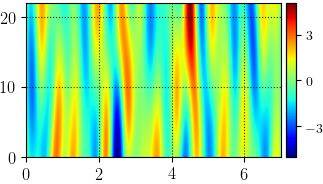
\includegraphics[width=.8\textwidth,height=.2\textheight]{MNG_ppoinitial}
\end{minipage}
\begin{minipage}[height=.2\textheight]{.5\textwidth}
\centering
\small{\texttt{(b)}} \\
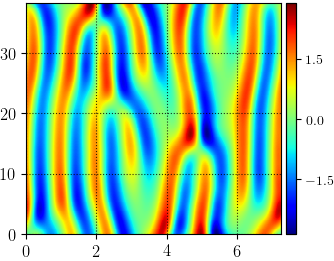
\includegraphics[width=.8\textwidth,height=.3\textheight]{MNG_ppofinal}
\end{minipage}
\begin{minipage}[height=.2\textheight]{.5\textwidth}
\centering
\small{\texttt{(c)}} \\
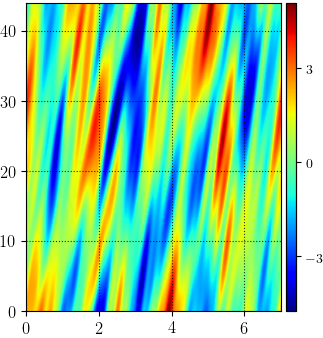
\includegraphics[width=.8\textwidth,height=.39\textheight]{MNG_rpoinitial}
\end{minipage}
\begin{minipage}[height=.2\textheight]{.5\textwidth}
\centering
\small{\texttt{(d)}} \\
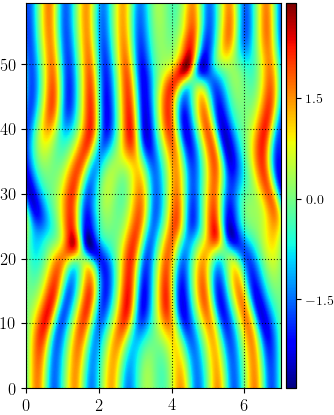
\includegraphics[width=.8\textwidth,height=.48\textheight]{MNG_rpofinal}
\end{minipage}
\caption{ \label{fig:KStrawl}
(a) Initial condition for \twot\ with shift-reflection symmetry, defined on
$\speriod{}=44,\period{}=44$ (fundamental domain). (b) Converged \twot\
resulting from optimization of (a), $\speriod{}\approx 45.58$,$\period{}\approx 76.46$.
(c) Initial condition with spatial translation symmetry (shown in co-moving reference frame),
$\speriod{}=44,\period{}=44$. (d) Converged \twot\ resulting from optimization
of (c), $\speriod{}\approx 44.01$,$\period{}\approx,59.36$,}
\end{figure}

There are alternative methods which we
predict would have greater efficiencies
in terms of convergence.
By taking our library of solutions we can average their
\spt\ Fourier modes to create a template for the ``typical'' spectrum
that different classes of solutions exhibit. There are a number
of things that must be handled carefully, for instance,
for different \spt\ domain sizes the \Fcs\ do not represent
modes with the same frequency so they do not directly map onto
one another. The best way of accounting for the differing domain
sizes is the ``bin'' the frequency data is a method
akin to a histogram. There is another alternative
idea which is hypothetically possible but unclear
whether it is realized.
Our hypothesis is that every \twot\ is comprised of
shadowing of small \spt\ \twots, a topic which we discuss in
much more detail in \refsect{sect:tiles}. If this is
indeed the case then this should be exhibited by
the spectra of the general solution. Therefore,
an additional manner initial conditions could be
created is to take utilize the spectra of just the
tiles.
Looking to the future it has also been put forward that \spt\ methods
will be able to better capitalize on advances in computing, specifically
the increase in number of computational cores\rf{WGBGQ13}.
The idea is that in the future computational speed will not be able
to keep pace with the number of computational cores, and so
one should begin to think in parallel.
Our \spt\ formulation is in the same spirit but unfortunately
we are precluded from the same subdivision that Wang \etal\rf{WGBGQ13} use
because we use periodic boundary conditions. Their idea
is that by subdividing \spt\ domains into subdomains, the equations
being solved locally on each subdomain, in parallel, and then combined
together at their boundaries implicitly. This does not allow for
periodic boundary conditions implying that a \spt\ Fourier basis
is a poor choice. One would want to switch
to either a finite difference scheme or (preferably) a Chebyshev
collocation method in conjunction with new boundary conditions.
On the other side of this discussion, the main
disadvantage of the \spt\ formulation is the increased
number of variables.
To represent the discretization of
a point in the dynamical system's state space we
might use $M$ spatial Fourier modes. The \spt\ equivalent would
be a $N \times M$ \spt\ discretization. In addition, the convergence of
the temporal modes is typically slower than spatial modes because
the time derivatives are of first order. Therefore, not
only must we increase the number of variables by a factor of $N$
but also $N$ will typically be larger than $M$, implying a practical
lower bound of $M^2$ for the number of computational variables. This
quadratic scaling is of course dramatically worse than the $\mathcal{O}(M)$
scaling. The effect of this increase in dimensionality precludes
us from using direct methods such as Newton's method,
as the number of entries of any linearization matrix scales approximately
like $M^4$.



In summary, our \spt\ formulation involves no time integrations and is
thus free of their exponential instabilities. It allows us to
find a large number of numerically accurate \twots\
with comparatively small computational cost.
This allows
us to test our main hypothesis which describes larger \spt\ \twots\
in terms of fundamental ``tiles'' which we shall see in \refsect{sect:tiles}
and \refsect{sect:glue}. Namely, we will demonstrate that it is possible to
take combine subdomains of known solutions to find even more solutions.
These methods exemplify the general idea of a self-sustaining process
in Navier-Stokes flows, in which the general process of sustained
turbulence is described via the interactions of a few fundamental
patterns realized in fluid flows\rf{W97}. By construction their
self-sustaining processes are time dependent; for us however, we
merely are combining patterns and see which are admissible.
Their model is an attempt to describe complex behavior with a
relatively simple model.
%This may be a stretch
This type of modeling can loosely
be interpreted as a dimensional reduction because it attempts
to describe temporal patterns with a small number of ``variables''.
Our \spt\ combinations however do not suffer any reduction in complexity
as we use exact \spt\ solutions of \refeq{e-ks} to describe
all possible patterns.

Know how, does it work

So far we have motivated a {\spt} theory of turbulence
which replaces unstable dynamics with \spt\ patterns.
We formulate these ideas using the \KSe, creating a number of
new numerical techniques in the process.
The following section describes the results of our numerical investigation.

Before we began searching for {\po}s in earnest, we first
tested the efficacy of the {\spt} numerical methods %\MNG{reference section here}
using known {\po}s \rf{SCD07}.
The first test was to find solutions of \refeq{e-Fks} using coarse {\spt} discretizations.
This is important because the main limiting factor
for {\spt} methods is the number of {\cdofs}; the entire orbit must be
kept in the computational memory. It is imperative that we be able to
find {\po}s with coarse resolutions, otherwise the problem is not computationally
feasible unless we consider more advanced computing resources.
Each test performed simply rediscretized a known solution to create an coarse
initial guess, which was then pass to our numerical methods.
In all of the tests we performed, the guess converged to the
``same'' {\po} that it originated from.
Technically, they are not returning
to exactly the same {\po}, but rather, the same family of {\po}s. This
topic arises organically later on when we detail the existence
of continuous families of {\fpo}s, and so we leave the discussion until then.
These tests showed that we could now solve \refeq{e-Fks} with coarse
discretizations, however, using known solutions to perform these tests however
is not very convincing; therefore we then applied
to initial guesses created by adding a substantial amount of noise
to these known {\po}s.

The idea behind this test was simply to see whether or not
the noisy initial guess would converge.
At each field site in the discretization, we drew a value from a
normal distribution with mean zero and whose standard deviation was the
$L_{\infty}$ norm of the {\po}'s field. We only performed a single test
but the results were still  Not only did the
sum of the original field and the noise converge, it converged to the original {\po}
up to translations and small differences in periods.
This exceeded our expectations as the noise was much larger in magnitude
than the original {\po} itself.
Note that we did not include perturbations to the periods but
they remained unconstrained. This test case used a {\po}
with small periods, however, the extent of the noise made us
optimistic that initial guesses of poor quality could be used to find {\po}s.
After these two tests we began the search and collection of {\po}s.
This search applied the methods of \refsect{sect:intro} and
spanned all symmetry types and a range of domain sizes; specifically,
the periods were drawn from the intervals
$L \times T \in [22, 88] \times [20, 200]$.
As a reminder our hypothesis does not require the collection of exceptionally large {\po}s;
they must only be large enough to capture all unique fundamental patterns. If we believed
that this range of periods was insufficient we would have expanded our
search.


Disregarding a few outliers (to be discussed later) the vast majority of {\po}s in this collection
look more or less the same. More precisely, if one were to zoom in on a {\po} and examine
the local features and patterns in a small {\spt} window, neither
the global {\spt} symmetry nor the {\extent} would be ascertainable. This reinforced our belief that {\fpo}s are indeed universal and
can be used to explain all solutions.
The figure %\reffig{fig:waldo}
displays {\po}s of the four different
{\spt} symmetry classes that we considered in our investigation. We believe they are essentially
indistinguishable when only the fundamental domains are plotted (obviously if the symmetry
is visible they can be distinguished from one another).%\MNG{reference figure here}
%\begin{figure}
%\begin{minipage}[height=.05\textheight]{.3\textwidth}
%\centering \small{\texttt{(a)}\\
%\includegraphics[width=.3\textwidth,height=.1\textheight]{MNG_waldo1}
%\end{minipage}
%\begin{minipage}[height=.05\textheight]{.3\textwidth}
%\centering \small{\texttt{(b)}\\
%\includegraphics[width=.4\textwidth,height=.1\textheight]{MNG_waldo2}
%\end{minipage}
%\begin{minipage}[height=.05\textheight]{.3\textwidth}
%\centering \small{\texttt{(c)}\\
%\includegraphics[width=.4\textwidth,height=.1\textheight]{MNG_waldo3}
%\end{minipage}
%\begin{minipage}[height=.05\textheight]{.3\textwidth}
%\centering \small{\texttt{(d)}\\
%\includegraphics[width=.8\textwidth,height=.1\textheight]{MNG_waldo4}
%\end{minipage}
%\caption{ \label{fig:waldo}
%Four {\po}s which demonstrate the ubiquity of patterns irrespective of
%the global symmetry of the housing {\po}.
%}
%\end{figure}
Another means of developing our intuition regarding {\spt} patterns is
to look at the \textit{atypical} patterns of the \KSe.
This classification consists of three main categories: {\po}s which
are `too symmetric', contain `uncommon' patterns, or
which follow an \eqv\ for an extended time.
In dynamical systems context `outliers' is our blanket term for very isolated (unstable) solutions which would hardly ever realized.
Our searches find these outliers
because stability has no affect on the optimization problem.
This implies that our variational method also captures
`rare events', a notably hard problem that has utility in other situations. \MNG{mentioning this worthwhile (or accurate)?}

The usage of `outliers' as opposed to 'isolated' is because solutions exist continuous families
and hence are not `isolated'. Support for our claim that
they are not frequented often is that they are typically found
to exist in the antisymmetric subspace which is very unstable and hence not
visited for long periods of time.  % sources? Lorenz z axis analogy?
Originally we found {\po}s classified as outliers everywhere; but
it may be that they all exist in the antisymmetric subspace. This seems
contradictory if not for a particular computational detail.
It is possible to find antisymmetric solutions
without specifically constraining an initial guess to the antisymmetric subspace.
This is because an antisymmetric {\po}s have the same topology as other {\po}s;
it manifests only as a constraint on the {\Fcs}.
What does this mean? It depends
on the symmetries being compared but here are two examples. In figure %\MNG{figure reference here}
demonstrates a {\po} found with no imposed symmetry.
Another possibility occurs with shift-reflection invariant {\po}s. Due to
the nature of the constraints on the {\Fcs}, imposing shift-reflection symmetry
can also find even multiples of prime periods of antisymmetric {\po}s;
i.e. two, four, etc. repeats of antisymmetric solutions in time.
These aren't just assumptions either; these solutions can actually be converged to the
antisymmetric subspace if their reflection axes are restored, as seen in {}.
This demonstrates that {\po}s with discrete symmetries are simply special representatives
of their group orbit produced via translations.
This would have never been realized in the dynamical
systems context due to the instability of the antisymmetric subspace.%\MNG{is this actually a new revelation?}
%The solution %\reffig{rposlant}
%demonstrates a behavior that is not particularly common on smaller domain sizes.
%\subsubsection{Analysis of the library}
%examples of initial conditions and their converged results.
%examples depicting similar structures regardless of symmetry
%examples demonstrating repeats of the structures after a prescribed length
%examples of similar yet deformed structures / the structure's scales.
%\subsubsection{Outliers}
%Under resolved solutions
%Large equilibria solutions?

We have displayed {\po}s that we consider to be both typical and atypical.
Our intuition evolved to the point where we could identify {\fpo} candidates.
The notable property of these candidates is that they not only occur frequently throughout the
{\po} collection; they also occur frequently within individual {\po}s.
To further motivate the existence of
{\fpo}s as well as some initial guesses, we direct the reader to %\MNG{figure reference here}
where a very large time integrated trajectory (aperiodic in time)
is displayed. Notable in this figure is the {\spt}
frequency with which a single pattern occurs.

The first guess was the {\wiggle} which appears in% \MNG{figure reference here}
It very distinctly repeats twice with respect to time in
and is relatively small in spatial scale, containing only two notable wavelengths.

This was the inaugural search for a {\fpo} and so extra
care was taken in the clipping process \refsect{sect:intro}.
In this instance the clipping was done iteratively, finding
a sequence of progressively smaller {\po}s each of which contained the {\fpo}.
We now know that it is was possible to clip and converge {\fpo}s in a single clipping,
but this example is kept in its entirety to demonstrate additional utility.

The results of the {\wiggle} search are as displayed in %\MNG{figure reference here}
The final result was an antisymmetric {\fpo} whose velocity field on
the fundamental domain consisted of a wavelength or streak ``wiggling'', hence the name.
To check our work, comparison of this pattern with our {\po} collection was made.
While the {\wiggle} was converged in the antisymmetric subspace, the
pattern most often as a pair of wiggles.
As previously mentioned in the discussed of ``outlier'' {\po}s, the antisymmetric {\wiggle}
should be viewed as a special case of the continuous family of {\wiggle} solutions as
this case will never appear in actuality.

The collection of the {\wiggle} not only provided us with our first {\fpo} but also
provided us with an obvious guess for the second {\fpo}. If we look back
at the iterative clipping procedure that we just performed, %\MNG{figure reference here}
we see that the {\wiggle} is spatially adjacent to an additional,
single wavelength {\eqv}. %\MNG{figure reference here}
By appealing to the notion of {\spt} {\symbolic} we postulated that
this {\eqv} would be our second {\fpo}. Indeed, by clipping this
single wavelength {\eqv} from the original {\po} another {\fpo} was found,
which we now refer to as the {\streak}.

At this point we knew that our library was yet incomplete as we had not
captured the pattern emphasized in %large cutouts.
This pattern, now named the {\defect}, captures two very important physical processes (they
could be interpreted as two sides of the same coin, really). First, two spatially adjacent
wavelengths merge into a single wavelength. In the gap in space-time left behind by this
merger, a new wavelength emerges. The result is a new pair of wavelengths which
exhibit an approximate phase difference of a
half wavelength with the original pair (approximately a quarter of
the spatial period).
This {\defect} epitomizes two very important mechanisms of the \KSe:
fluctuations in global wavelength count and local spatial drift velocity.
Neither the {\streak} nor the {\wiggle} can account for
these behaviors, highlighting the importance of the {\defect}.
The actual search for the {\defect} was quite challenging relative to the other
{\fpo}s. Due to the spatial
shift it should be no surprise that the {\fpo} was assumed to be a {\rpo}.
Locating the {\defect} proved to be much more difficult than both the {\wiggle}
and {\streak}, in part due to the extra {\cdof} from the spatial shift.


\MNGedit{After our first search concluded, we believed that there were four unique {\fpo}s.
Upon further review two of these four {\fpo}s looked quite similar visually, leading us
to believe that they were related. This was verified by pseudo-arclength continuation using
the spatial period as the parameter. Continuation was performed until the spatial periods
of this {\fpo} pair were the same. By fixing the phases of the
{\Fcs} it is quite clear that these {\fpo}s are equivalent.
This brought about a revelation regarding
{\fpo}s that had been previously glossed over;
{\fpo}s exist in continuous families. In hindsight it could not have been
any other way. Shadowing by {\fpo}s is not an exact process;
clippings from larger trajectories always look similar but not identical. This
property is precisely captured by continuous families: which are
infinite sets of solutions related by continuous deformations.}

From a dynamical systems perspective
this is not shocking nor new as previous bifurcation analyses
track different branches of {\po}s.
The main effect of these families is that our {\symbolic}
now consists of a ``rubbery'' continuous alphabet, as opposed to a static discrete one.
For each symbol in any {\spt} {block}, the symbol now represents a continuous
family of {\fpo}s. To best illustrate the effect of this,
we delve into the continuous family of the {\defect}.
We display the numerical continuation of the defect as a
function of the spatial period noting
that there are other manners with which {\po}s can be continued. A collection of representatives
are displayed in {}. The main result of the investigation is
that the family is perhaps more properly parameterized
by the spatial shift parameter.
% more on defect family.

It might be accurate to say that all {\po}s
exist in continuous families \emph{because} {\fpo}s exist in
continuous families. This initially betrayed our intuition; in hyperbolic systems, {\po}s are
isolated solutions by virtue of their unstable manifolds. In any case each continuous
family seems to exist on a finite interval of spatial periods, punctuated by what are
presumed to be bifurcations. It could be that this assumption is incorrect and that we
are failing to track the correct branch of the solutions.
Exploration of the {\fpo} continuous families reduced the alphabet
to three. To reiterate; there may only be three {\fpo}s
needed to describe all solutions of the {\KSe}.

It is absolutely essential to understand the notion of continuous families of {\fpo}s
and so we summarize it here before moving on to the description of gluing results. We postulated
and then found a collection of {\fpo}s whose existence can ostensibly describe all solutions.
We believe that this collection consists of three unique {\fpo} continuous families.
We currently do not have a clear manner with which to develop a {\spt} {\symbolic}.
To begin the investigation, however, we can test our ideas by creating
{\spt} combinations of {\fpo}s. This is the aforementioned gluing method,
whose results shall now be described.


First as a proof of concept we reproduce a known solution by combining many small,
custom tailored components. Next, we demonstrate how to glue known {\po}s along a single spacetime dimension: either time or space.
Lastly, we glue {\spt} combinations of {\fpo}s to find {\po}s.
The first question we aimed to answer was ``Can a known solution be reproduced by combining many different clippings from
other solutions?''.  This is demonstrated in %reffig{}.
where a handmade {\spt} combination was used to create an initial guess for a specific {\po} which
is known to exist.

The resultant {\po} is essentially a reproduction of the target up to continuous family considerations. This prototype of the gluing method was developed concurrently with the search
for {\fpo}s. In this case the constituent pieces are not converged {\fpo}s but merely clippings from {\po}s not including the target. The success of this trial gave credence to the argument for {\po}s
existing as collections of {\fpo}s.
While this result was very encouraging it was also somewhat contrived.
The initial guess was hand tailored to be a rough approximation to the
targeted {\po}. Therefore we did not know whether this result would generalize.
The next step was to implement unsupervised gluing along a single continuous dimension.
In this context ``unsupervised'' implieds that the only decision
that is made is which {\po}s to glue together.
We focus on only gluing one pair of {\po}s at a time but also demonstrate
that this process can be applied iteratively.

We begin by temporally gluing {\po}s with small spatial periods,
a familiar notion to those cognizant of periodic orbit theory. Our computation
is completely different however as the spatial periods are allowed to differ
as well as freely vary.
Upon success we were able to find {\po}s with large temporal periods.
For instance, in %reffig
the final converged {\po} is a shift-reflection invariant orbit whose fundamental domain
has period $386.088... / 2$. Similarly in %reffig
is an examples of a converged {\rpo} with time period $231.419...$. These periods
are what we would expect if the gluing was properly functioning, as they are
approximately the sum of the periods of the original {\po}s.
These {\po}s are much longer than anything we have seen
in the literature which again exemplifies how robust
our {\spt} methods are.

In line with our identical treatment of space and time we also glue {\po}s spatially.
The figures %reffig reffig
show exactly this where the original {\po}s, their gluing, and the resultant {\po} are shown.
In %reffig{MNGppo12spaceglue}
two {\po}s with shift-reflection symmetry were chosen to be glued in space.

Much like the clipping process we can also iteratively glue to create a sequence of
progressively larger {\po}s. To demonstrate this, we glue the result
from the previous example to yet another {\po} with shift-reflection symmetry. Originally
the choice was made to only glue in a symmetry preserving manner; shift-reflection symmetric
orbits were only glued to other shift-reflection symmetric orbits, and the result was
also constrained to have shift-reflection symmetry. It was realized that there
was no real motivation behind this choice and so this requirement was removed, such that
it is not applied in the next section when discussing gluing {\fpo}s together.


Showing that we can both glue in space and time we proceed to
the ultimate method: gluing {\spt} combinations of {\fpo}s.
To review our motivation, let us again explain the process in terms of {\symbolic}.
The initial guesses can be thought of as symbolic blocks, where each symbol
is representative of a {\fpo}'s continuous family. Quite literally, the symbols are replaced
by these {\fpo}s to construct an initial guess; an approximation to a possible {\po}.
We elect to use a static set of
representative {\fpo}s for each of these substitutions with no motivation other
than simplicity. Specifically: the {\defect},
{\wiggle}, and {\streak} displayed in %reffig final tiles.

To deem each gluing as a success, they must satisfy a {\symbolic} requirement
in addition to numerical convergence. Namely, the initial guesses must converge
to a {\po} which has the ``correct'' symbolic representation.
That is, it must be contain the {\fpo}s which befits its construction.
Yet again, however, we are forced to rely upon visual inspection to validate our results.
First, we provide examples which we claim are successful under our new requirement.
Next, are examples of numerical success but ``symbolic failure''.
The existence of this class of outcomes, in combination with our lack of verification of results,
contributes to the challenge of making the {\symbolic}. Specifically,
this prevents us from determining the correct grammar of
the {\symbolic}; the rules which dictate whether each {block} is admissible {\po} or not.

In summary we have shown that it is possible to use our techniques to find {\po}s by construction,
clipping and gluing. In essence
clipping and gluing are inverses of one another, however, gluing is
typically more difficult than clipping due to the inherent differences in complexity. In practice,
we usual clip in a single step but glue iteratively.
Currently we have a very surface level method and there are currently many unknowns in regards to best practices. Essentially we have made the simplest choices which result in the gluing method to be
numerically well defined. While these results are very informative they leave us with more open
questions than we started with \refsect{sect:future}. The future is bright, however, as the number of potential improvements seems to be limited only by our creativity.

Discounting the time it took to produce the codes used for
the computations, it did not take much effort to complete the
collection of \twots. This search was performed over intermediately
sized domains and all symmetry types.

The first test of the ideas was to converge coarse discretizations
of known solutions. When converged using shooting type methods, the
number of discrete time steps numbers in the thousands. When converged
using other variational techniques such as the Newton descent method, \rf{LanThesis}
mentions using upwards of 512 to 1024 discrete time points. Meanwhile, the method
proposed here can converge solutions on very coarse discretizations orders of magnitude smaller
than these other methods. This is slightly disingenuous as the shooting type method does
not require all of the points to be maintained in memory; this is merely an
argument that the memory requirements for \spt\ methods do not need to be nearly
as large as one might imagine. This reduces even further if imposing discrete symmetries;
a common occurrence in flows such as pipe and and plane Couette flows \rf{GHWC07}.
The familiarity with finite difference methods leads to another foreseeable counter argument;
coarse discretization which do not resolve the appropriate physical scales lead to nonsensical
solutions, regardless of whether or not they converge. This is exactly the case; if the problem
were to be composed of finite differences in physical space. The coarse discretization in
Fourier space is sufficient to resolve all physically relevant modes a quick visual inspection is
typically sufficient; this can be done by interpolating a finer grid via zero padding.
If skepticism remains an alternative would be to alternative between zero padding and converging.
This works but it will change the \spt\ dimensions if they remain free parameters and so
the lattice dimension is best increased in small increments. It is possible to perform
this type of extension to a very large dimension but it is very hard to decrease the error;
we recommend using this as an error density such that the absolute tolerance becomes
$NM \cdot 10^{-15}$ instead of $10^{-15}$. This remains a qualitative value but there
is evidence that the tolerance need not be machine precision for the calculations at least
in the spatiotemporal setting which lacks dynamical instability. As a test of practicality of
this bound a numerical experiment was ran which attempted to converge a known solution using
a discretization which dwarfed the original. After a finite number of gradient descent steps
a spatial strip was taken from the approximate solution and integrated in time to test whether
or not this would reproduce the solution. A successful test increased a \spt\ discretization
of size $[64, 32]$ to $[4096, 512]$. Not many tests were run so this could be an indication
of sampling bias, but it was informative at least in regards to whether or not this formulation
could work for higher dimensional equations.

Once this preliminary testing was completed, we started trawling the solution space
for \twots. The parameter ranges employed for the search varied, but the typical ranges were
$L \in [22, 66]$, $T \in [20, 180]$. The typical lattice dimensions over these ranges
were $N\times M \in [32, 128] \times [32, 64]$.

The typical pattern for finding a solution was as follows. An initial field with very
large magnitude of the cost function, upwards of $\approx 10^{10}$, is annealed by the descent
algorithm.
This uses the method described in %\refsect{how}


 typically ending at the maximum step limit instead of the numerical
tolerance. The annealed approximation is then passed
to the least-squares backtracking algorithm. The damping
typically starts high until the the approximation nears a \twot with
the last few steps typically being undamped.
``Rough patches'' are also common during the least-squares
backtracking routine; this term represents local regions where the damping increases
presumeably due to increased curvature of the cost function.

The computation times to find solutions ranged from seconds to tens of minutes, depending
heavily on the dimensionality of the discretization. The solutions which converged the fastest always resulted
from smaller solutions which did not take much time at all to complete the descent algorithm;
essentially they would be immediately passed to the least-squares algorithm.


\begin{figure}
\begin{minipage}[height=.05\textheight]{.5\textwidth}
\centering
\small{\texttt{(a)}} \\
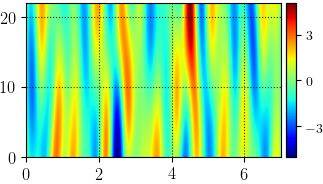
\includegraphics[width=.8\textwidth,height=.2\textheight]{MNG_ppoinitial}
\end{minipage}
\begin{minipage}[height=.2\textheight]{.5\textwidth}
\centering
\small{\texttt{(b)}} \\
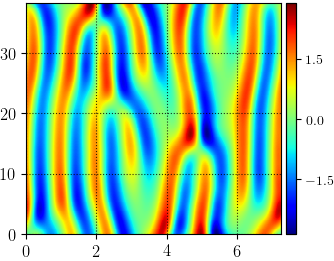
\includegraphics[width=.8\textwidth,height=.3\textheight]{MNG_ppofinal}
\end{minipage}

\caption{ \label{fig:ppo1}
(a) Initial condition for \twot\ with shift-reflection symmetry, defined on
$\speriod{}=44,\period{}=44$ (fundamental domain). (b) Converged \twot\
resulting from optimization of (a), $\speriod{}= 45.58\dots$,$\period{}= 76.46\dots$.
(c) Initial condition with spatial translation symmetry (shown in co-moving reference frame),
$\speriod{}=44,\period{}=44$. (d) Converged \twot\ resulting from optimization
of (c), $\speriod{} = 44.01\dots$,$\period{}=59.36\dots$,}
\end{figure}

In \reffigs{fig:ppo1, fig:rpo1} we demonstrate a

\begin{figure}
\begin{minipage}[height=.05\textheight]{.5\textwidth}
\centering
\small{\texttt{(a)}} \\
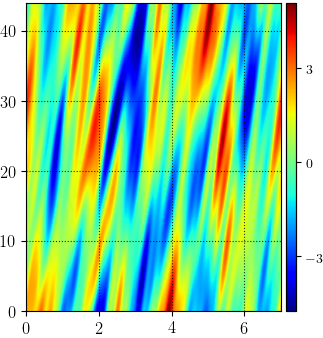
\includegraphics[width=.8\textwidth,height=.39\textheight]{MNG_rpoinitial}
\end{minipage}
\begin{minipage}[height=.2\textheight]{.5\textwidth}
\centering
\small{\texttt{(b)}} \\
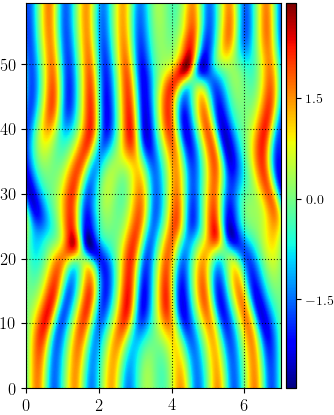
\includegraphics[width=.8\textwidth,height=.48\textheight]{MNG_rpofinal}
\end{minipage}
\caption{ \label{fig:rpo1}
(a) Initial condition with spatial translation symmetry
(displayed in co-moving reference frame),
$\speriod{}=44,\period{}=44$. (b) Converged \twot\ resulting from optimization
of (c), $\speriod{} = 44.01\dots$,$\period{}=59.36\dots$,}
\end{figure}

%more examples, anti, eqva, different kinds of initial condition generation?

%Tiles
After examination of our library of solutions we determined that there are
only a small number of fundamental patterns. We have tentatively named
these patterns after the basic physical processes they represent.
The first tile is actually defined with $T=0$

They can be described by the
following physical processes.


Upon convergence of the
guesses for these tiles, this number reduced even further upon realization
that some of the guesses belong to the same continuous family.

Despite our best efforts to determine the opposite, no continuous symmetry
was found that explains these continuous families of tiles.

The interpretation of these families is that instead of having a unique, finite set of tiles
we instead

The most frequent patterns, that is, those which are presumably the best tile
candidates are relatively simple to describe in terms of physical processes.
This description is best carried out in the context of spatial waves present
in each solution. The natural length scale of the equations

The most unstable wavelength, however, seems to mediate the interaction between these
waves.
The ``most'' fundamental of the tiles is what we have denoted as the streak tile.


Our
naming convention appeals to similar shapes witnessed in fluid simulations.
It has been argued that the natural length scale of the problem is the wavelength
corresponding to the most unstable mode. Visual inspection of arbitrary
solutions shows a slightly more detailed story best described as a tug-of-war between two
different length scales. The most unstable wavelength results from the linearized
spectrum; while informative it does not encapsulate the full story. Luckily the
tiles The number of pronounced (amplitude above a threshold)
wavelengths varies over time, seemingly oscillating between these two different scales.

The transition to the
most unstable wavelength seems to be a transient phenomenon that accounts for
the destruction of wavelengths via collision. This is not simply linear
superposition of waves but the linear affects can be
The equilibria



\MNGedit{
Specifically, we need a collection {\po}s
defined over a range of spatial and temporal periods. This is achieved by creating
initial guesses whose periods exist on some finite range of values.
Once a library of {\po}s has been created, we identify the most frequently
occurring patterns which, by our claim,
are regions of spacetime shadowed by {\fpo}s. Once a handful of {\fpo}
candidates are decided upon, the next step in the {\spt} pipeline is to convert
them into initial guesses; we do so with a technique we call `clipping'.}
\MNGedit{2020-05-15}{
The search for {\po}s combines the initial guess creation of \refsect{sect:guesses}
with the numerical optimization methods \refsect{sect:descent}, \refsect{sect:leastsquares}.
For the numerical methods, a handful of parameters are required such as the step limit
and tolerance. Our typical choices, noting that they are likely suboptimal, are as follows:
the tolerance of the cost function for the gradient descent was $J = 10^{-4}$
and the step limit was set to a multiple of the dimension, either $16NM$ or $32NM$.
This means that if either \refeq{e-cost} $J < 10^{-4}$ or the step limit
is reached, then the descent method terminates, and the guess is passed to the
least-squares implementation.
The ``heavy lifting'' was delegated to the least-squares method
with backtracking. The threshold for termination was originally set to double
floating point precision but over time this was relaxed to incorporate the {\cdof}, i.e.
the current tolerance is on the order of $(NM)*10^{-15}$; and the step limit, $500$.
For those familiar with Newton methods, this number of steps appears like overkill at first, but the
allowance of backtracking negatively impacts the rate of convergence.
    } 
% proof of concept of tiling, set up the making it exact.
\section{Clipping}
Once identified, the most frequently recurring patterns are used
as initial guesses in the search for {\fpo}s. Specifically, a {\spt} window is
fit to the pattern such that the state within the window is as close to being
doubly periodic as possible. Once the best window is found, the region of space-time
is clipped from the {\po} and used as an initial condition.
Hitherto, clipping has always been performed manually. As a consequence there
is substantial variability in clipping quality;
multiple clippings may be necessary to find a single {\fpo}.



It is one thing to claim that certain \spt\ \twots\ are the building blocks
of turbulence for the \KSe. It is
another thing entirely to put our money where our mouth is by actually using them in this manner. We would like to remind the audience that the ability to construct and find solutions in this manner
has not been witnessed in the literature. With this in mind our choices should
be treated as preliminary ones; it is entirely possible and likely that
many improvements could be made.
Much like the clipping process used to find tiles combining solutions in space-time,
the overarching idea of gluing is straightforward and intuitive.
Specifically, the tiles represent the
Brillouin zone, fundamental domain, unit cell of a lattice, etc.
of each fundamental \twot.
The general case is that we have a general $s_n \times s_m$ sized mosaic of tiles.
The admissibility of the gluing is determined by the (currently unknown) symbolic
dynamics. Gluing is only well defined if the lattices being combined have the same
number of grid points along the gluing boundary.
This creates a problem, however, as
different tiles will have different \spt\ dimensions $\speriod{},\period{}$ because
they are fundamentally different solutions.
This actually helps provide a precise meaning to the term ``gluing''.
Gluing is a method of creating initial conditions which approximates
a non-uniform rectangular lattice (combination of tiles) as uniform.
This of course introduces local error which depends on the grid size; therefore
there should not be an extreme discrepancy between the \twots\ or tiles being glued.
With this in mind, we simply rediscretize and concatenate the new lattices.
The dimensions of the new lattice are determined by the sum or average of
the original dimensions.
For example, if gluing two tiles together in time, the new period would be
$\period{} = \period{1} + \period{2}$ but the new spatial period is
$\speriod{} = \frac{\speriod{1} + \speriod{2}}{2}$.
In this case the number of spatial grid \emph{points} and temporal grid \emph{spacing}
should be the same. There are many more complicated alternatives, limited only by
the imagination.

It is actually recommended to not use descent methods for small dimension problems; Newton
converges too quickly to not use and with backtracking the region of convergence can
increase substantially.


Another option would be to simply decrease the allowed damping, thus causing more failures,
but run more searches in parallel.

Searching through the library of collected \twots\ led to a number of candidates
for fundamental tiles. This was a natural result of picking out the most frequent patterns
that occur spatiotemporally. This section focuses on the numerical process of finding tiles;
it is almost self explanatory. The claim is that the tiles are \twots\ which shadow larger \twots.
Therefore we should be able to find these tiles by numerically clipping them out of larger \twots\
and then passing them to the same numerical routine used to converge the larger \twot. If
the original \twot\ has dimensions $x \in [0, L_0]$ and $t \in [0, T_0]$ and is defined on
a lattice $[\xm, \tn]$ then the process is as follows. Find the approximate domain on which
the shadowing occurs $x \in [0, x_{i}-x_{j}]$, $t \in [0, t_{p}-t_{j}]$; translational invariance allows
us to start from the origin. The tile is then defined on the corresponding lattice of size
$M', N' = M \frac{x_{i}-x_{j}}{L}, N * \frac{t_{i}-x_{j}}{T}$.
$M', N'$ are always taken to be even numbers for reasons specific to our computational codes.
This leaves us with a field defined on this subset of the original lattice;
this will never be doubly periodic. The discontinuities which result from
the clipping are handled by simple truncation of the higher
frequency \spt\ \Fcs.


If possible, clippings were made such that the result minimized the discontinuities at
the boundary. This is both numerically beneficial but also motivated by the notion
of tiles representing shadowing of small \twots.

This process suffices to find tiles such that any other methods that
improve the initial conditions are ignored.

The only step left is to converge these initial conditions numerically
just like how was done with the larger \twots.
This process continues until we believe that we have captured all
fundamental solutions depicting in our library of \twots.
This appeals to our intuition which begs the question: is there a quantitative
manner to know whether our tile collection is complete? The answer to this
question arises naturally as a consequence of the next component of this numerical method,
namely, the gluing of \twots\ and tiles.


It is one thing to claim that certain \spt\ \twots\ are building blocks; it is
another thing all together to be able to actually use them in this manner. We would like to
remind the audience that the ability to construct and find solutions in this manner
has not been witnessed in the literature. With this in mind our choices should
be treated as preliminary ones; it is entirely possible and likely that
many improvements could be made. This
description covers both the implementation that worked for us for the \spt\ \KSe,
as well as some alternatives.


\MNGedit{The idea behind clipping is very intuitive. Given any {\po}, a clipping is a window
of space-time which is used as an initial guess.
Clipping may be applied iteratively until ultimately a {\fpo} is reached.
The reverse process, combining {\fpo}s together
to create initial guesses for find larger orbits is also possible; in fact,
this technique is the crux of our theory. We denote this combination process as
gluing, a name which again appeals to our intuition.}

%\subsubsection{clip}
As a reminder, our claim is that the tiles are \twots\ which shadow larger \twots.
Therefore we should be able to converge subdomains which have been numerically clipped out
of larger \twots. After visual inspection, we believed the number of fundamental tiles to
be small. Therefore, a precise and unsupervised algorithm for clipping was not developed.
Instead the only criteria we abided by is that the clipping must include the tile being
sought after; of course, clippings that were closer to being doubly periodic were sought after.
For the original \twot\ with dimensions $x \in [0, \speriod{0}]$ and $t \in [0, \period{0}]$ defined on a lattice, the
clipping can be described as follows. Find the approximate domain on which
the shadowing occurs and then literally extract the subregion of the parent lattice,
setting the new {\spt} dimensions according to the smaller lattice. In other words,
the same grid spacing was maintained throughout this procedure.
This process in combination with our numerical methods was sufficient
for finding tiles.

As a reminder, our claim is that the tiles are \twots\ which shadow larger \twots.
Therefore we should be able to converge subdomains which have been numerically clipped out
of larger \twots. After visual inspection, we believed the number of fundamental tiles to
be small. Therefore, a precise and unsupervised algorithm for clipping was not developed.
Instead the only criteria we abided by is that the clipping must include the tile being
sought after; of course, clippings that were closer to being doubly periodic were sought after.
For the original \twot\ with dimensions $x \in [0, \speriod{0}]$ and $t \in [0, \period{0}]$ defined on a lattice, the
clipping can be described as follows. Find the approximate domain on which
the shadowing occurs and then literally extract the subregion of the parent lattice,
setting the new {\spt} dimensions according to the smaller lattice. In other words,
the same grid spacing was maintained throughout this procedure.
This process in combination with our numerical methods was sufficient
for finding tiles.


% how to properly find FPO's.
% how to continue po's, families of po's
\section{Pseudo-arclength continuation}
\input{chapters/techniques/continuation}
\section{Gluing}
% siminos/spatiotemp/chapter/glue.tex
% $Author: predrag $ $Date: 2020-05-22 16:09:57 -0400 (Fri, 22 May 2020) $

%  \section{Combining {\spt} solutions}
%  \label{sect:glue}

%Possible figures
%Idea behind gluing
%schematic for gluing
%step by step gluing in space (multiple figures instead of one)
%step by step gluing in time (multiple figures instead of one)
%various \twots\ resulting from gluing
%general picture of gluing in its extension to fluid dynamics?

In \refsect{sect:tiles} we described a method to use tiles
to find solutions motivated by symbolic dynamics. We can also
apply this technique to any \twots\ even though it's not as
well motivated as combining tiles. Because of this
we can use our library of solutions from \refsect{sect:trawl}
to find even more solutions. Another detail we have not discussed is
how to combine solutions such that the converged combination has
the same symmetry as the initial \twots. For example, we can
combine two shift-reflection invariant \twots\ to find a larger
shift-reflection invariant \twot. We will
now describe the process of gluing \twots\ to find larger \twots.
Instead of allowing any number of \twots\ in the initial combination
(like in tiling) we will only glue a single pair of \twots\ at a
time. Progressively larger \twots\ can be made by iteratively gluing
\twots\ together. This distinction between tiling and gluing is because
in tiling there was symbolic dynamic motivation which allows for
any sized symbolic blocks. It might be better to converge symbolic
subdomains in the tiling procedure but we leave that to future
investigations. Of course we want to mention that similarly to our tiling procedure
there is likely much room for improvement of these numerical methods.

Currently, we always glue solutions with identical symmetries because
the final \twot\ is also assumed to have this symmetry. The rationale
behind this is that (for discrete \spt\ symmetries) the \spt\ Fourier coefficients
exist in subspaces of the full set of \spt\ Fourier coefficients. Therefore,
throughout the entire gluing process we constrain ourselves to
a particular symmetry subspace. This requires the gluing
to be done in a symmetry preserving manner. For discrete symmetries
it is sufficient to work with solution's fundamental domains, \ie, the
\spt\ subdomains that can reproduce the entire \twot\ via
symmetry operations. For example, the fundamental domain
for a reflection invariant solution is half of the spatial domain, because the
other half can be acquired by reflection.
The required decisions to be made before the gluing
process are: which dimension we will use to glue
the \twots\ and which \twots\ to glue.
The choice of the solutions, as
previously stated, are required to have the same symmetry.
Other factors that play a role in this decision
are the \spt\ domain sizes of each \twot.
In practice, the transverse dimension to the gluing direction corresponding
to the boundary between \twots\ should have similar magnitudes.
In other words, imagine we want to
glue two solutions defined on $[\speriod{0},\period{0}]$
and $[[\speriod{1},\period{1}]$ and we choose to glue
in the spatial direction.
Because we have decided to glue in space the discrepancy between
$\period{0}$ and $\period{1}$ cannot be too large lest the initial error will
be large. This error of course results from \twots\ tangent's depending on $\speriod{},\period{}$ so
of course if we only have approximations to $\speriod{},\period{}$ we will
only have an approximation to a \twot\ even though the fields individually correpond
to solutions of \refeq{e-ks}. The difference in
dimensions should be bounded above by some unknown value but in practice
this magnitude of this bound can be quite large. This leniency is once again
ascribed to the efficacy of our numerical methods.
We direct the reader to the results displayed in
    \PC{2019-12-06}{
    References `fig:MNGppo12space\_glue'
    `fig:MNGppo123space\_glue' `fig:MNG\_ppoLargeTspaceglue'
    `fig:MNG\_rpoLargeTtimeglue'
    undefined
    }\PCedit{
??%\reffig{fig:MNGppo12space_glue}
,
??%\reffig{fig:MNGppo123space_glue}
,
?? %\reffig{fig:MNG_ppoLargeTspaceglue},
and
??%\reffig{fig:MNG_rpoLargeTtimeglue}
    }
to get a sense of the possibilities of
this gluing method. We highlight
    \PCedit{
??%\reffig{fig:MNGppo123space_glue}
    }
because
the gluing was successful even though the periods differed by a factor of two.

Now that the general idea is in place we shall proceed to explain
the numerical steps in the \twot\ gluing process.
The search for \twots\ in \refsect{sect:trawl} and the tilings of \refsect{sect:tiles}
has already shown that the initial condition can afford to be inaccurate.
There are two main contributions to the error just like the tiling process:
discontinuities at the gluing boundaries and incorrect tangent magnitudes
from errors in $[\speriod{},\period{}]$.
First we perform the usual spectral padding to interpolate a much finer
{\spt} grid so that any cutting and pasting is more precise.
The interpolation is also performed in such a
manner such that their discretizations respect the aspect ratios of
the initial \twots.
That is to say, if one solution is twice as long
(in either space or time) as the other, then the longer solution will have
twice as many discretized point in that dimension. Mathematically
it's the simple relation $\frac{\period{i}}{\period{j}}=\frac{\period{N_i}}{\period{N_j}}$.
If the solutions have continuous symmetry then we are also free to perform
\spt\ rotations such that the difference between the boundaries is minimized.
Spatial rotations are not afforded by solutions with discrete reflection
and shift-reflection symmetries because of the reflection axis.
For these solutions with discrete symmetry we can, however, work with
fundamental domains and then reproduce the full glued \twot\ by
symmetry operation. For reflection invariant \twots\ this corresponds
to taking half of the spatial extent and for shift-reflection invariant
\twots\ it is half of the temporal extent. This
subdivision into and subsequent selection of reflection equivariant subdomains
allows us to construct the approximate fundamental domain of our new \twot.
Numerically, this new fundamental domain is formed by conjoining
the two initial fundamental domains in physical space by concatenating
the two dimensional arrays containing the field information.
To produce the best initial condition as determined by the
cost functional \refeq{e-costfunctional} we also have to take
the ordering of the fundamental domains in account. The combination
which has the smallest value of the cost functional is taken to be the
representative of this particular gluing.
In case its not clear what is meant by combinations
we will explain with an example. There are eight ways of
combining two fundamental domains
with reflection symmetry. These eight combinations arise
from the spatial ordering as well as which fundamental domains to choose from
the original \twots.
The fundamental domains of each initial \twot\ are equivalent conceptually
but not numerically; it matters which is chosen to be combined.
Once the original \twots\ or fundamental domains therefrom are combined,
we apply a smoothing procedure to create a better initial condition.
The smoothing is handled by truncating the high frequency \spt\ \Fcs.
This is a simple way
of reducing the effect of the Gibbs phenomenon; the effect of the boundary
discontinuities on the \spt\ \Fcs. Other possible methods are
mentioned in \refsect{sect:tiles} and so are not repeated here. The main
takeaway is that the numerical methods seem effective enough to not
warrant a complicated procedure to combine solutions.
Still, this added effort has currently not been worth
pursuing due to the strength of the developed numerical methods, but
it is good to keep an additional procedure handy if our goals
change and require better initial conditions.
The gluing of \twots\ and fundamental domains of \twots\ are shown
schematically in \reffig{fig:MNGspaceglue}, \ref{fig:MNGtimeglue},
\ref{fig:MNGreflxglue}, \ref{fig:MNGshiftreflxglue} and \ref{fig:MNGshiftrefltglue}.


\begin{figure}
\begin{minipage}[height=.1\textheight]{.45\textwidth}
\centering
\small{\texttt{(a)}} \\
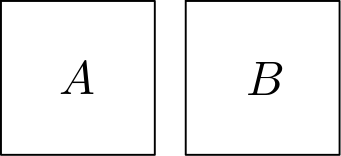
\includegraphics[width=.45\textwidth,height=.07\textheight]{MNG_AB}
\end{minipage}
\begin{minipage}[height=.1\textheight]{.45\textwidth}
\centering
\small{\texttt{(b)}} \\
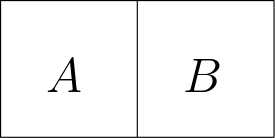
\includegraphics[width=.45\textwidth,height=.07\textheight]{MNG_ABx}
\end{minipage}
\caption{ \label{fig:MNGspaceglue}
Depiction of spatial gluing for \twots\ with spatial translation symmetry.
(a) Initial \twots\ and (b) \twots\ with correct gluing order.
}
\end{figure}


\begin{figure}
\begin{minipage}[height=.1\textheight]{.45\textwidth}
\centering
\small{\texttt{(a)}} \\
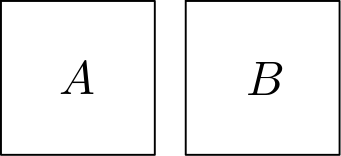
\includegraphics[width=.45\textwidth,height=.07\textheight]{MNG_AB}
\end{minipage}
\begin{minipage}[height=.1\textheight]{.45\textwidth}
\centering
\small{\texttt{(b)}} \\
\includegraphics[width=.225\textwidth,height=.15\textheight]{MNG_ABt}
\end{minipage}
\caption{ \label{fig:MNGtimeglue}
Depiction of temporal gluing for \twots\ with either spatial translation symmetry
or reflection symmetry. (a) Initial
\twots\ and (b) \twots\ with correct gluing order.
}
\end{figure}


\begin{figure}
\begin{minipage}[height=.1\textheight]{.45\textwidth}
\centering
\small{\texttt{(a)}} \\
\includegraphics[width=.45\textwidth,height=.07\textheight]{MNG_AB}
\end{minipage}
\begin{minipage}[height=.1\textheight]{.45\textwidth}
\centering
\small{\texttt{(b)}} \\
\includegraphics[width=.45\textwidth,height=.07\textheight]{MNG_ABreflx}
\end{minipage}
\caption{ \label{fig:MNGreflxglue}
Depiction of spatial gluing for \twots\ with reflection symmetry. (a) Initial
\twots\ and (b) \twots\ with correct gluing order.
}
\end{figure}


\begin{figure}
\begin{minipage}[height=.1\textheight]{.45\textwidth}
\centering
\small{\texttt{(a)}} \\
\includegraphics[width=.45\textwidth,height=.07\textheight]{MNG_AB}
\end{minipage}
\begin{minipage}[height=.1\textheight]{.45\textwidth}
\centering
\small{\texttt{(b)}} \\
\includegraphics[width=.5\textwidth,height=.035\textheight]{MNG_AFBFshiftrefl}
\end{minipage}
\centering
\begin{minipage}[height=.1\textheight]{.6\textwidth}
\centering
\small{\texttt{(c)}} \\
\includegraphics[width=.45\textwidth,height=.09\textheight]{MNG_ABshiftreflx}
\end{minipage}
\caption{ \label{fig:MNGshiftreflxglue}
Depiction of spatial gluing for \twots\ with shift-reflection symmetry. (a) Initial
\twots\ and (b)fundamental symmetry domains (c) post-gluing initial condition for
shift-reflection \twot. Superscripts in this instance stand for ``left'' and
``right'' halves of the corresponding fundamental domain $A_F$
}
\end{figure}

\begin{figure}
\begin{minipage}[height=.1\textheight]{.45\textwidth}
\centering
\small{\texttt{(a)}} \\
\includegraphics[width=.45\textwidth,height=.07\textheight]{MNG_AB}
\end{minipage}
\begin{minipage}[height=.1\textheight]{.45\textwidth}
\centering
\small{\texttt{(b)}} \\
\includegraphics[width=.5\textwidth,height=.035\textheight]{MNG_AFBFshiftrefl}
\end{minipage}
\centering
\begin{minipage}[height=.1\textheight]{.45\textwidth}
\centering
\small{\texttt{(c)}} \\
\includegraphics[width=.25\textwidth,height=.20\textheight]{MNG_ABshiftreflt}
\end{minipage}
\caption{ \label{fig:MNGshiftrefltglue}
Depiction of temporal gluing for \twots\ with shift-reflection symmetry. (a) Initial
\twots\ (b) fundamental symmetry domains and (c) post-gluing initial condition for
shift-reflection \twot.
}
\end{figure}

\begin{figure}
\centering
\begin{minipage}[height=.4\textheight]{.66\textwidth}
\centering
\includegraphics[width=.7\textwidth,height=.6\textheight]{MNGppo12space_glue}
\end{minipage}
\caption{ \label{fig:MNGppo12spaceglue}
Spatial gluing of the two shortest shift-reflection
\twots. The sizes of the fundamental domains of these
\twots\ are
$[\speriod{1},\period{1}]=[3.5\cdots,20.50\cdots]$
and
$[\speriod{2},\period{2}]=[3.5\cdots,28.66\cdots]$
respectively.
The result is a
shift-reflection \twot\ with
$[\speriod{1,2},\period{1,2}]=[6.79\cdots,24.82\cdots]$
fundamental domain.
}
\end{figure}


\begin{figure}
\begin{minipage}[height=.4\textheight]{.99\textwidth}
\centering
\includegraphics[width=.99\textwidth,height=.66\textheight]{MNGppo123space_glue}
\end{minipage}
\caption{ \label{fig:ppo123spaceglue}
Gluing procedure which spatially combines the third shortest (period) shift-reflection
invariant
$[\speriod{3},\period{3}]=[3.5\cdots,64.70\cdots]$
\twot\
 with the resultant shift-reflection invariant \twot\
from
\PCedit{reffig{fig:ppo12spaceglue}} %2019-12-06
with
$[\speriod{1,2},\period{1,2}]=[6.79\cdots,24.82\cdots]$
fundamental domain.
This results in another shift-reflection
\twot\ with the
$[\speriod{1,2,3},\period{1,2,3}]=[10.53\cdots,68.84\cdots]$
 fundamental domain.
The dramatic change between the last
two panels is presumably an effect of the
discrepancy between the temporal period of
the constituent solutions.
}
\end{figure}
    \PC{2019-12-06}{
    Reference `fig:ppo12spaceglue' undefined in \reffig{fig:ppo123spaceglue}
    }

\begin{figure}
\centering
\begin{minipage}[height=.4\textheight]{.66\textwidth}
\centering
\includegraphics[width=.7\textwidth,height=.6\textheight]{MNG_ppolargeTspaceglue}
\end{minipage}
\caption{ \label{fig:MNGppo12spaceglue1}
Spatial gluing of the two shortest shift-reflection
\twots. The sizes of the fundamental domains of these
\twots\ are
$[\speriod{1},\period{1}]=[3.5\cdots,20.50\cdots]$
and
$[\speriod{2},\period{2}]=[3.5\cdots,28.66\cdots]$
respectively.
The result is a
shift-reflection \twot\ with
$[\speriod{1,2},\period{1,2}]=[6.79\cdots,24.82\cdots]$
fundamental domain.
}
\end{figure}


\begin{figure}
\centering
\begin{minipage}[height=.4\textheight]{.66\textwidth}
\centering
\includegraphics[width=.7\textwidth,height=.6\textheight]{MNG_rpoLargeTtimeglue}
\end{minipage}
\caption{ \label{fig:MNGppo12spaceglue2}
Spatial gluing of the two shortest shift-reflection
\twots. The sizes of the fundamental domains of these
\twots\ are
$[\speriod{1},\period{1}]=[3.5\cdots,20.50\cdots]$
and
$[\speriod{2},\period{2}]=[3.5\cdots,28.66\cdots]$
respectively.
The result is a
shift-reflection \twot\ with
$[\speriod{1,2},\period{1,2}]=[6.79\cdots,24.82\cdots]$
fundamental domain.
}
\end{figure}


    \PC{2019-12-06}{
    Reference `fig:ppo12spaceglue' undefined
    }\PCedit{
refFig{fig:ppo12spaceglue}
    }
and \reffig{fig:ppo123spaceglue}
both demonstrate the spatial gluing
of shift-reflection \twots. In fact, \reffig{fig:ppo123spaceglue}
uses the result of
    \PCedit{
 reffig{fig:ppo12spaceglue}
    }
as an initial
condition. We chose to display these two gluing examples
because they are demonstrative of how gluing can be performed
iteratively to find progressively larger solutions.

\MNG{2019-10-22}{This part is unclear; I'm trying to say that 1-D symbolic
itineraries are much easier to interpret than spatiotemporal blocks...
unfinished and incoherent as of now}

Our tiling and gluing methods constitute ways that larger \twots\
can be found by utilizing smaller \twots. This notion of combinations
has been performed temporally\rf{DV03} as a natural
consequence of symbolic dynamics. In other words, for a dynamical system
with a chaotic attractor it is somewhat straightforward to interpret
symbolic itineraries; they represent visitation of different partitioned
areas of the attractor parameterized with time.
The idea to do this with
respect to spatial dimensions is desirable in the context of minimal
computational cells of plane Couette for instance. Combining solutions
in a \spt\ manner is a whole other beast as symbolic blocks are
hard to interpret in the context of state space.

% small to large FPO
\section{Tiling}

\begin{figure}
\begin{minipage}[height=.05\textheight]{.5\textwidth}
\centering
\includegraphics[width=.8\textwidth,height=.2\textheight]{MNG_orbitblocktile_flow_chart}
\end{minipage}
\caption{ \label{fig:MNG_flowchart}
This flow chart represents the order that is required to make
{\spt} constructions. The flow from orbits to prime orbits to fundamental
orbits represents the process of searching for solutions and then clipping
out the fundamental tiles. Once the fundamental tiles are converged, the
fundamental tiles are well defined (the space-time on which the fundamental
orbit sits) as well as the fundamental blocks (the names that we assign
to the unique pattern found in the fundamental orbit). In order to glue,
there are three requirements, the prime configuration of blocks, the
prime tile that they are defined on, and the
approximate state that exists on the prime tile. Only after the prime
tile and prime block are in place can the fundamental orbits be
laid out on the prime tile. With this, an approximate solution that is
shadowed by a prime orbit is made. By converging this shadowed orbit
we arrive at the prime orbit it is shadowed by. Symmetry operations and
space-time periodicity then produce the entire (global) orbit.
}
\end{figure}


%%%%%%%%%%%%%%%%
% Chapter 5
%%%%%%%%%%%%%%%%
\chapter{Results}
\label{c-results}
%% i.e. noise and frankenstein.
\section{Preliminary results}


\begin{figure}[ht]
\begin{minipage}[height=.32\textheight]{.45\textwidth}
\centering \small{\texttt{(a)}}
\includegraphics[width=\textwidth,height=.32\textheight]{MNGspacetimeinit1}
\end{minipage}
\begin{minipage}[height=.32\textheight]{.45\textwidth}
\centering \small{\texttt{(b)}}
\includegraphics[width=\textwidth,height=.32\textheight]{MNGspacetimefinal1}
\end{minipage}
\caption{ \label{fig:MNGspacetime11}
(a) Initial condition of the 32-by-32 space-by-time discretization of \ppo{10.2}:
$(L_0,\period{0}) = (L_0, 2\period{p_0})= (22,20.5057459345)$.
(b) Resulting spatiotemporal fixed point
$(L_p,2\period{p}) =  (22.0000104401, 20.5057499188)$
}
\end{figure}

\begin{figure}
\begin{minipage}[height=.32\textheight]{.45\textwidth}
\centering \small{\texttt{(a)}}
\includegraphics[width=\textwidth,height=.32\textheight]{MNGvndspaceinit2}
\end{minipage}
\\
\begin{minipage}[height=.32\textheight]{.45\textwidth}
\centering \small{\texttt{(b)}}
\includegraphics[width=\textwidth,height=.32\textheight]{MNGvndtimefinal2}
\end{minipage}
\begin{minipage}[height=.32\textheight]{.45\textwidth}
\centering \small{\texttt{(c)}}
\includegraphics[width=\textwidth,height=.32\textheight]{MNGvndspacefinal2L}
\end{minipage}
\caption{ \label{fig:MNGspaceandtime1}
(a) Initial condition of the 16-by-16 space-by-time discretization of
\rpo{16.31}. $L_0 = 22$.
(b) Resulting periodic orbit after variational {newton descent} in time $L =
22, T = 15.7444884386$,
(c) resulting periodic orbit after variational {newton descent} in space.
%%%lost the number for final spatial size will need to run code again.
}
\end{figure}


\begin{figure}[ht]
\begin{minipage}[height=.32\textheight]{.45\textwidth}
\centering \small{\texttt{(a)}}
\includegraphics[width=\textwidth,height=.32\textheight]{MNG_T100L44_init}
\end{minipage}
\begin{minipage}[height=.32\textheight]{.45\textwidth}
\centering \small{\texttt{(b)}}
\includegraphics[width=\textwidth,height=.32\textheight]{MNG_T100L44_final}
\end{minipage}
\caption{ \label{fig:MNG_spacetime_smoothed}
(a) Smoothed and $\bar{L}=2\pi\sqrt{2}$ modulated ``noise''
initialized on a spacetime domain
$(L_0,T_0)=(5\bar{L},100)=(44.4,100)$. Initial residual $F^2 = 1808$.
(b) Resultant \twot\ after meeting tolerance
$F(\tau)^2= 1.86<10^{-3} F(0)^2$.
$(L_f,T_f)=(43.066,105.08) = (L_0 - 1.363,T_0 + 5.08)$.
The computation took only 7 CPU seconds on my laptop.
}
\end{figure}

\begin{figure}
\begin{minipage}[height=.32\textheight]{.45\textwidth}
\centering \small{\texttt{(a)}}
\includegraphics[width=\textwidth,height=.32\textheight]{MNG_T500L888_init}
\end{minipage}
\\
\begin{minipage}[height=.32\textheight]{.45\textwidth}
\centering \small{\texttt{(b)}}
\includegraphics[width=\textwidth,height=.32\textheight]{MNG_T500L888_final}
\end{minipage}
\begin{minipage}[height=.32\textheight]{.45\textwidth}
\centering \small{\texttt{(c)}}
\includegraphics[width=\textwidth,height=.32\textheight]{MNG_T500L888_capped}
\end{minipage}
\caption{ \label{fig:MNG_spacetime_capped}
(a) Smoothed noise initialized on a spacetime domain $T=500$,
$L=100\,\bar{L} \approx 889$, where $\bar{L}=2\pi\sqrt{2}$.
Initial residual $F^2 = 16635$
(b) Resultant spatiotemporal field after one-hundred thousand adjoint descent
steps $F^2_f = 3.66$, $T_f = 682.62$, $L_f=828.31$.
(c) The same $u(x,t)$ as in (b), except with the displayed values constrained
between $-2.4 \leq u(x,t) \leq 2.4$. Computation time was approximately an hour
and ten minutes.
}
\end{figure}


\begin{figure}
\begin{minipage}[height=.05\textheight]{.3\textwidth}
\centering \small{\texttt{(a)}}\\
\includegraphics[width=.3\textwidth,height=.1\textheight]{MNG_streak}
\end{minipage}
\begin{minipage}[height=.05\textheight]{.3\textwidth}
\centering \small{\texttt{(b)}}\\
\includegraphics[width=.4\textwidth,height=.1\textheight]{MNG_hookondefecterg}
\end{minipage}
\begin{minipage}[height=.05\textheight]{.3\textwidth}
\centering \small{\texttt{(c)}}\\
\includegraphics[width=.4\textwidth,height=.1\textheight]{MNG_halfdefecterg}
\end{minipage}
\begin{minipage}[height=.05\textheight]{.3\textwidth}
\centering \small{\texttt{(d)}}\\
\includegraphics[width=.8\textwidth,height=.1\textheight]{MNG_tiling_subdomain0}
\end{minipage}
\begin{minipage}[height=.05\textheight]{.3\textwidth}
\centering \small{\texttt{(e)}}\\
\includegraphics[width=.8\textwidth,height=.1\textheight]{MNG_tiling_subdomain1}
\end{minipage}
\begin{minipage}[height=.05\textheight]{.3\textwidth}
\centering \small{\texttt{(f)}}\\
\includegraphics[width=.8\textwidth,height=.1\textheight]{MNG_tiling_subdomain2}
\end{minipage}
\begin{minipage}[height=.1\textheight]{.35\textwidth}
\centering \small{\texttt{(g)}}\\
\includegraphics[width=.8\textwidth,height=.28\textheight]{MNG_tiling_twosubdomains}
\end{minipage}
\begin{minipage}[height=.15\textheight]{.3\textwidth}
\centering \small{\texttt{(h)}}\\
\includegraphics[width=\textwidth,height=.36\textheight]{MNG_tiling_fundamental}
\end{minipage}
\begin{minipage}[height=.15\textheight]{.3\textwidth}
\centering \small{\texttt{(i)}}\\
\includegraphics[width=\textwidth,height=.36\textheight]{MNG_tiling_initial}
\end{minipage}

\caption{ \label{fig:tilingschematic}
Demonstration of how to construct an initial condition corresponding to a specific
\spt\ symbolic block. (a),(b) and (c) together are the set of tiles used for all
other plots in this figure. (d) is a subdomain comprised of two copies of (a) and one copy of (b). (e) is a subdomain comprised of two copies of (a) and one copy of
the reflection of (b). (f) is a subdomain comprised of two copies of (a) and a
single copy of (c). The last row of figures demonstrate how to combine (d),(e),
and (f). (g) is the combination of (d) and (e). (h) is the combination of (d),(e)
and (f) (equivalently, (g) and (f)). Lastly (i) is the smoothed version of (h) which will serve as the initial condition.
}
\end{figure}

\begin{figure}
\begin{minipage}[height=.05\textheight]{\textwidth}
\centering
\includegraphics[width=1.0\textwidth,height=.2\textheight]{MNG_noise}
\end{minipage}
\caption{ \label{fig:MNGnoise}
(a) Original, converged \twot\ $[\speriod{}=21.99...,
\period{}=20.50...]$,
(b) aperiodic noise taken from standard normal distribution,
multiplied by
the $L_{\infty}$ norm of (a), (c) is the sum of (a) and (b),
(d) is the
\twot\ that (c) converges to, $[\speriod{}=22.18...,
\period{}=20.58...]$ .
}
\end{figure}

For a sense of how much noise is added, the maximum and
minimum values of
the fields in \reffig{fig:MNGnoise} are
(a) $\approx \pm 2.47$ and (c) $\approx \pm 8$. All four
fields are included
in a single figure to make it easier to have them share the
color legend. 
\section{Orbits}
\input{chapters/results/hunt_results}
%\input{chapters/results/large_results} %if I can drum up something quickly using orbithunter
\section{Orbit clipping and fundamental periodic orbits}

\begin{figure}
\begin{minipage}[height=.3\textheight]{.32\textwidth}
\centering \small{\texttt{(a)}}
\includegraphics[width=1.0\textwidth,height=.25\textheight]{MNG_HOD_init}
\end{minipage}
\begin{minipage}[height=.3\textheight]{.32\textwidth}
\centering \small{\texttt{(b)}}
\includegraphics[width=1.0\textwidth,height=.29\textheight]{MNG_HOD_STREAK_init}
\end{minipage}
\begin{minipage}[height=.3\textheight]{.32\textwidth}
\centering \small{\texttt{(c)}}
\includegraphics[width=1.0\textwidth,height=.17\textheight]{MNG_HOD_STREAK_final}
\end{minipage}
\caption{ \label{fig:MNGhodstreak}
(a) Initial condition from \reffig{fig:MNG_HOD_tile} that converges to
a solution that is believed to be a numerical continuation of (b) from \reffig{fig:MNGsymb11}. (b) An initial condition
resulting from concatenating a streak-pair with (a), that
numerically converges to (c).
}
\end{figure}

\begin{figure}
\begin{minipage}[height=.3\textheight]{.32\textwidth}
\centering \small{\texttt{(a)}}
\includegraphics[width=1.0\textwidth,height=.25\textheight]{MNG_HD_init}
\end{minipage}
\begin{minipage}[height=.3\textheight]{.32\textwidth}
\centering \small{\texttt{(b)}}
\includegraphics[width=1.0\textwidth,height=.29\textheight]{MNG_HD_STREAK_final}
\end{minipage}
\begin{minipage}[height=.3\textheight]{.32\textwidth}
\centering \small{\texttt{(c)}}
\includegraphics[width=1.0\textwidth,height=.17\textheight]{MNG_HD_STREAK_final}
\end{minipage}
\caption{ \label{fig:MNGhdstreak}
(a) Initial condition that has not been shown to numerically converge. (b) An initial condition
resulting from concatenating a streak-pair with (a), that
numerically converges to (c).
}
\end{figure}



\begin{figure}
\begin{minipage}[height=.4\textheight]{.5\textwidth}
\centering \small{\texttt{(a)}}\\
\includegraphics[width=.5\textwidth,height=.5\textheight]{MNG_halfdefect_defect_initial}
\end{minipage}
\begin{minipage}[height=.4\textheight]{.5\textwidth}
\centering \small{\texttt{(b)}}\\
\includegraphics[width=.5\textwidth,height=.5\textheight]{MNG_defect_guess}
\end{minipage}
\begin{minipage}[height=.1\textheight]{\textwidth}
\centering \small{\texttt{(c)}}\\
\includegraphics[width=.14\textwidth,height=.1\textheight]{MNG_defect}
\end{minipage}
\caption{ \label{fig:defect}
(a)
$[\speriod{a},\period{a}]=[3.50\cdots,94.59\cdots]$ fundamental domain
of an already computed \twot\ with spatial translation symmetry.
(b)
The clipped-out $[\speriod{b},\period{b}]=[2,17]$ subdomain used the
initial guess for the fundamental domain of a shift-reflect symmetric tile.
(c)
The converged $[\speriod{c},2\period{c}]=[2.07\cdots,18.46\cdots]$ \twot\
with spatial translation symmetry.
}
\end{figure}

\begin{figure}
\begin{minipage}[height=.4\textheight]{.5\textwidth}
\centering \small{\texttt{(a)}}\\
\includegraphics[width=.5\textwidth,height=.5\textheight]{MNG_halfdefect_defect_initial}
\end{minipage}
\begin{minipage}[height=.4\textheight]{.5\textwidth}
\centering \small{\texttt{(b)}}\\
\includegraphics[width=.5\textwidth,height=.5\textheight]{MNG_halfdefect_guess}
\end{minipage}
\begin{minipage}[height=.1\textheight]{\textwidth}
\centering \small{\texttt{(c)}}\\
\includegraphics[width=.14\textwidth,height=.12\textheight]{MNG_halfdefect}
\end{minipage}
\caption{ \label{fig:halfdefect}
(a)
$[\speriod{a},\period{a}]=[3.50\cdots,94.59\cdots]$ fundamental domain
of an already computed \twot\ with spatial translation symmetry.
(b)
The clipped-out $[\speriod{b},\period{b}]=[2.2,20]$ subdomain used the
initial guess for the fundamental domain of a shift-reflect symmetric tile.
(c)
The converged $[\speriod{c},2\period{c}]=[2.07\cdots,15.46\cdots]$ \twot\
with spatial translation symmetry.
}
\end{figure}

\begin{figure}
\begin{minipage}[height=.4\textheight]{.5\textwidth}
\centering \small{\texttt{(a)}}\\
\includegraphics[width=.5\textwidth,height=.5\textheight]{MNG_halfdefect2_initial}
\end{minipage}
\begin{minipage}[height=.4\textheight]{.5\textwidth}
\centering \small{\texttt{(b)}}\\
\includegraphics[width=.5\textwidth,height=.5\textheight]{MNG_halfdefect2_guess}
\end{minipage}
\begin{minipage}[height=.1\textheight]{\textwidth}
\centering \small{\texttt{(c)}}\\
\includegraphics[width=.14\textwidth,height=.1\textheight]{MNG_halfdefect2}
\end{minipage}
\caption{ \label{fig:halfdefect2}
(a)
$[\speriod{a},\period{a}]=[3.50\cdots,85.73\cdots]$ fundamental domain
of an already computed \twot\ with \spt\ shift-reflection symmetry.
(b)
The clipped-out $[\speriod{b},\period{b}]=[2.6,17]$ subdomain used the
initial guess for the fundamental domain of a shift-reflect symmetric tile.
(c)
The converged $[\speriod{c},\period{c}]=[2.06\cdots,19.92\cdots]$ \twot\
with spatial translation symmetry.
}
\end{figure}

\begin{figure}
\begin{minipage}[height=.1\textheight]{.5\textwidth}
\centering \small{\texttt{(a)}}\\
\includegraphics[width=.5\textwidth,height=.1\textheight]{MNG_hook_initial}
\end{minipage}
\begin{minipage}[height=.1\textheight]{.5\textwidth}
\centering \small{\texttt{(b)}}\\
\includegraphics[width=.5\textwidth,height=.1\textheight]{MNG_hook_guess}
\end{minipage}
\begin{minipage}[height=.1\textheight]{\textwidth}
\centering \small{\texttt{(c)}}\\
\includegraphics[width=.16\textwidth,height=.1\textheight]{MNG_hook}
\end{minipage}
\caption{ \label{fig:hook}
(a)
$[\speriod{a},\period{a}]=[3.50\cdots,10.25\cdots]$ fundamental domain
of an already computed \twot\ with \spt\ shift-reflection symmetry.
(b)
The clipped-out $[\speriod{b},\period{b}]=[2.1,10.5]$ subdomain used the
initial guess for the fundamental domain of a shift-reflect symmetric tile.
(c)
The converged $[\speriod{c},\period{c}]=[2.08\cdots,9.22\cdots]$  \twot\
with spatial translation symmetry.
}
\end{figure}

\begin{figure}
\begin{minipage}[height=.3\textheight]{.5\textwidth}
\centering \small{\texttt{(a)}}\\
\includegraphics[width=.6\textwidth,height=.4\textheight]{MNG_gap_initial}
\end{minipage}
\begin{minipage}[height=.3\textheight]{.5\textwidth}
\centering \small{\texttt{(b)}}\\
\includegraphics[width=.6\textwidth,height=.4\textheight]{MNG_gap_guess}
\end{minipage}
\begin{minipage}[height=.1\textheight]{\textwidth}
\centering \small{\texttt{(c)}}\\
\includegraphics[width=.12\textwidth,height=.13\textheight]{MNG_gap}
\end{minipage}
\caption{ \label{fig:gap}
(a)
$[\speriod{a},\period{a}]=[4.25\cdots,54.13\cdots]$ fundamental domain
of an already computed \twot\ with \spt\ shift-reflection symmetry.
(b)
The clipped-out $[\speriod{b},\period{b}]=[2.7,15]$ subdomain used the
initial guess for the fundamental domain of a shift-reflect symmetric tile.
(c)
The converged $[\speriod{c},\period{c}]=[2.90\cdots,17.95\cdots]$ full
reflection symmetric \twot.
}
\end{figure}

\begin{figure}
\begin{minipage}[height=.2\textheight]{.5\textwidth}
\centering \small{\texttt{(a)}}\\
\includegraphics[width=.8\textwidth,height=.5\textheight]{MNGgapzero}
\end{minipage}
\begin{minipage}[height=.2\textheight]{.5\textwidth}
\centering \small{\texttt{(b)}}\\
\includegraphics[width=.8\textwidth,height=.18\textheight]{MNGgapone}
\end{minipage}
\begin{minipage}[height=.2\textheight]{.5\textwidth}
\centering \small{\texttt{(c)}}\\
\includegraphics[width=.6\textwidth,height=.18\textheight]{MNGgaptwo}
\end{minipage}
\begin{minipage}[height=.2\textheight]{.48\textwidth}
\centering \small{\texttt{(d)}}\\
\includegraphics[width=.5\textwidth,height=.18\textheight]{MNGgapthree}
\end{minipage}
\caption{ \label{fig:KStileextraction}
Sequential subdomain extraction to find tiles.
(a) A {\po} from the collection of new solutions
$[\speriod{a},\period{a}]=[4.25\cdots,54.12\cdots]$.
By taking progressively smaller subdomains (b)-(d) and numerically
converging them to \twots\ at each step, we are able to
find the smallest subdomain of (a) which can be converges
to a \twot, namely (d).
(b)$[\speriod{b},\period{b}]=[4.16\cdots,18.93\cdots]$
(c)$[\speriod{c},\period{c}]=[2.79\cdots,17.14\cdots]$
(d)$[\speriod{d},\period{d}]=[1.39\cdots,17.14\cdots]$
}
\end{figure}
\section{Continuous families}
dsadsadsa
\section{Gluing results}


%Gluing
It should be noted that previously we claimed that
there are only three tiles. This is actually disingenuous because when we use tiles
in gluing access to their group orbit is used; that is, any symmetry copy or member
of their continuous family can be used. It is the tile's neighbors which
determines which family member is used in the gluing process.

There are many uses for the process of gluing; the most important being the
eventually explanation of infinite space-time by virtue of \spt\ symbolic
dynamics

\begin{figure}
\centering
\begin{minipage}[height=.4\textheight]{.66\textwidth}
\centering
\includegraphics[width=.7\textwidth,height=.6\textheight]{MNGppo12space_glue}
\end{minipage}
\caption{ \label{fig:MNGppo12spaceglue}
Spatial gluing of the two shortest shift-reflection
\twots. The sizes of the fundamental domains of these
\twots\ are
$[\speriod{1},\period{1}]=[3.5\cdots,20.50\cdots]$
and
$[\speriod{2},\period{2}]=[3.5\cdots,28.66\cdots]$
respectively.
The result is a
shift-reflection \twot\ with
$[\speriod{1,2},\period{1,2}]=[6.79\cdots,24.82\cdots]$
fundamental domain.
}
\end{figure}


\begin{figure}
\begin{minipage}[height=.4\textheight]{.99\textwidth}
\centering
\includegraphics[width=.99\textwidth,height=.66\textheight]{MNGppo123space_glue}
\end{minipage}
\caption{ \label{fig:ppo123spaceglue}
Gluing procedure which spatially combines the third shortest (period) shift-reflection
invariant
$[\speriod{3},\period{3}]=[3.5\cdots,64.70\cdots]$
\twot\
 with the resultant shift-reflection invariant \twot\
from
\PCedit{reffig{fig:ppo12spaceglue}} %2019-12-06
with
$[\speriod{1,2},\period{1,2}]=[6.79\cdots,24.82\cdots]$
fundamental domain.
This results in another shift-reflection
\twot\ with the
$[\speriod{1,2,3},\period{1,2,3}]=[10.53\cdots,68.84\cdots]$
 fundamental domain.
The dramatic change between the last
two panels is presumably an effect of the
discrepancy between the temporal period of
the constituent solutions.
}
\end{figure}


\begin{figure}
\centering
\begin{minipage}[height=.4\textheight]{.66\textwidth}
\centering
\includegraphics[width=.7\textwidth,height=.6\textheight]{MNG_ppolargeTspaceglue}
\end{minipage}
\caption{ \label{fig:MNGppo12spaceglue1}
Spatial gluing of the two shortest shift-reflection
\twots. The sizes of the fundamental domains of these
\twots\ are
$[\speriod{1},\period{1}]=[3.5\cdots,20.50\cdots]$
and
$[\speriod{2},\period{2}]=[3.5\cdots,28.66\cdots]$
respectively.
The result is a
shift-reflection \twot\ with
$[\speriod{1,2},\period{1,2}]=[6.79\cdots,24.82\cdots]$
fundamental domain.
}
\end{figure}


\begin{figure}
\centering
\begin{minipage}[height=.4\textheight]{.66\textwidth}
\centering
\includegraphics[width=.7\textwidth,height=.6\textheight]{MNG_rpoLargeTtimeglue}
\end{minipage}
\caption{ \label{fig:MNGppo12spaceglue2}
Spatial gluing of the two shortest shift-reflection
\twots. The sizes of the fundamental domains of these
\twots\ are
$[\speriod{1},\period{1}]=[3.5\cdots,20.50\cdots]$
and
$[\speriod{2},\period{2}]=[3.5\cdots,28.66\cdots]$
respectively.
The result is a
shift-reflection \twot\ with
$[\speriod{1,2},\period{1,2}]=[6.79\cdots,24.82\cdots]$
fundamental domain.
}
\end{figure}
\section{Tiling results}


\begin{figure}
\begin{minipage}[height=.4\textheight]{.5\textwidth}
\centering \small{\texttt{(a)}}\\
\includegraphics[width=.3\textwidth,height=.15\textheight]{MNG_01_initial}
\end{minipage}
\begin{minipage}[height=.4\textheight]{.5\textwidth}
\centering \small{\texttt{(b)}}\\
\includegraphics[width=.3\textwidth,height=.18\textheight]{MNG_01_final}
\end{minipage}
\caption{ \label{fig:block01}
(a) Initial \spt\ field for the one-by-two symbolic block given by \refeq{e-block01}
(b) \twoT\ resultant from numerically converging (a),
$[\speriod{b},\period{b}]=[3.13\cdots,20.84\cdots]$
}
\end{figure}

\begin{figure}
\begin{minipage}[height=.4\textheight]{.5\textwidth}
\centering \small{\texttt{(a)}}\\
\includegraphics[width=.4\textwidth,height=.15\textheight]{MNG_001_initial}
\end{minipage}
\begin{minipage}[height=.4\textheight]{.5\textwidth}
\centering \small{\texttt{(b)}}\\
\includegraphics[width=.4\textwidth,height=.23\textheight]{MNG_001_final}
\end{minipage}
\caption{ \label{fig:block001}
(a) Initial \spt\ field for the one-by-three symbolic block given by \refeq{e-block001}
(b) \twoT\ resultant from numerically converging (a),
$[\speriod{b},\period{b}]=[4.12\cdots,23.15\cdots ]$.
}
\end{figure}




% Example that shows transformation of gap to merger
\begin{figure}
\begin{minipage}[height=.4\textheight]{.5\textwidth}
\centering \small{\texttt{(a)}}\\
\includegraphics[width=.4\textwidth,height=.15\textheight]{MNG_000_220_initial}
\end{minipage}
\begin{minipage}[height=.4\textheight]{.5\textwidth}
\centering \small{\texttt{(b)}}\\
\includegraphics[width=.4\textwidth,height=.23\textheight]{MNG_000_220_final}
\end{minipage}
\caption{ \label{fig:block001}
(a) Initial \spt\ field for the one-by-three symbolic block given by \refeq{e-block001}
(b) \twoT\ resultant from numerically converging (a),
$[\speriod{b},\period{b}]=[4.12\cdots,23.15\cdots ]$.
}
\end{figure}

\begin{figure}
\begin{minipage}[height=.4\textheight]{.5\textwidth}
\centering \small{\texttt{(a)}}\\
\includegraphics[width=.4\textwidth,height=.15\textheight]{MNG_000_101_initial}
\end{minipage}
\begin{minipage}[height=.4\textheight]{.5\textwidth}
\centering \small{\texttt{(b)}}\\
\includegraphics[width=.4\textwidth,height=.23\textheight]{MNG_000_101_final}
\end{minipage}
\caption{ \label{fig:block000_101}
(a) Initial \spt\ field for the one-by-three symbolic block given by \refeq{e-block001}
(b) \twoT\ resultant from numerically converging (a),
$[\speriod{b},\period{b}]=[4.12\cdots,23.15\cdots ]$.
}
\end{figure}

By looking at the set of converged gluings it lacks the pattern corresponding
to a gap being adjacent to a merger, spatially.
Indeed, in almost every

Here are some examples,

% Example of finding something too symmetric/shows conservation of wavenumber
%\begin{figure}
%\begin{minipage}[height=.4\textheight]{.5\textwidth}
%\centering \small{\texttt{(a)}}\\
%\includegraphics[width=.4\textwidth,height=.15\textheight]{MNG_22_11_initial}
%\end{minipage}
%\begin{minipage}[height=.4\textheight]{.5\textwidth}
%\centering \small{\texttt{(b)}}\\
%\includegraphics[width=.4\textwidth,height=.23\textheight]{MNG_22_11_final}
%\end{minipage}
%\caption{ \label{fig:block001}
%(a) Initial \spt\ field for the one-by-three symbolic block given by \refeq{e-block001}
%(b) \twoT\ resultant from numerically converging (a),
%$[\speriod{b},\period{b}]=[4.12\cdots,23.15\cdots ]$.
%}
%\end{figure}

\begin{figure}
\begin{minipage}[height=.4\textheight]{.5\textwidth}
\centering \small{\texttt{(a)}}\\
\includegraphics[width=.4\textwidth,height=.15\textheight]{MNG_12_21_initial}
\end{minipage}
\begin{minipage}[height=.4\textheight]{.5\textwidth}
\centering \small{\texttt{(b)}}\\
\includegraphics[width=.4\textwidth,height=.23\textheight]{MNG_12_21_final}
\end{minipage}
\caption{ \label{fig:block12_21}
(a) Initial \spt\ field for the one-by-three symbolic block given by \refeq{e-block001}
(b) \twoT\ resultant from numerically converging (a),
$[\speriod{b},\period{b}]=[4.12\cdots,23.15\cdots ]$.
}
\end{figure}

This process depends on the neighbors of the tiles as well; it seems to be primarily
influenced by spatial neighbors. For instance, in

%\begin{figure}
%\begin{minipage}[height=.4\textheight]{.5\textwidth}
%\centering \small{\texttt{(a)}}\\
%\includegraphics[width=.4\textwidth,height=.15\textheight]{MNG_002_210_initial}
%\end{minipage}
%\begin{minipage}[height=.4\textheight]{.5\textwidth}
%\centering \small{\texttt{(b)}}\\
%\includegraphics[width=.4\textwidth,height=.23\textheight]{MNG_002_210_final}
%\end{minipage}
%\caption{ \label{fig:block002_210}
%(a) Initial \spt\ field for the one-by-three symbolic block given by \refeq{e-block001}
%(b) \twoT\ resultant from numerically converging (a),
%$[\speriod{b},\period{b}]=[4.12\cdots,23.15\cdots ]$.
%}
%\end{figure}

\begin{figure}
\begin{minipage}[height=.05\textheight]{.5\textwidth}
\centering
\small{\texttt{(a)}} \\
\includegraphics[width=.8\textwidth,height=.2\textheight]{MNG_streak_merger_initial}
\end{minipage}
\begin{minipage}[height=.2\textheight]{.5\textwidth}
\centering
\small{\texttt{(b)}} \\
\includegraphics[width=.8\textwidth,height=.3\textheight]{MNG_streak_merger}
\end{minipage}
\caption{ \label{fig:streakmerger}
(a) Initial condition composed of three streaks and an region of zeros,
imbued on a {\spt} domain approximating the known tile's domain size.
(b) The tile that (a) converges to.
}
\end{figure}

 


\chapter{Conclusions and Future Work}
\label{c-conclusion}
%% siminos/xiong/thesis/proposal/tex/proposal.tex
% $Author: xiong $ $Date: 2015-09-03 13:21:45 -0400 (Thu, 03 Sep 2015) $

\section{Plan for future work}
\label{sec:future}

\subsection{Dimension of inertial manifold}
We have only tested the method described in sec.~\ref{subsec:LDIM}
to investigated the dimension of inertial manifold in
1-dimensional \KSe, but we think this method can be applied to
other turbulent systems as well, for example \cGLe, 2-d or 3-d
Navier-Stokes equation. The point we conduct such research to other
systems in the next step
 is that
usually the mathematical proof of existence of inertial manifold
sheds
limited information about its exact dimension. Moreover,
for systems like
3-d Navier-Stokes, the existence of inertial manifold is still
unknown, so the experiments investigating decoupling in the
tangent space by \Fv s can serve as a valuable tool to provide
accurate enough information about the local geometry of inertial
manifold ahead of strict mathematical statements.
Also, this information can help engineers to use the appropriate
resolution in the numerical turbulence simulation.

\subsection{Cycle expansions for \cqcGLe}
We have found quite a few \reqv s in 1-d \cqcGLe\ and converted
the dynamics into the symmetry-reduced space. The next step
is trying to find \po s or \rpo s inside this system and
hopefully build the symbolic dynamics according to the
geometry of this hierarchy of \po s.

with this set of \po s, cycle expansion can be applied to \Fd\
\eqref{Z(s)} with interesting physical quantity such as diffusion rate as
the observable. Therefore, our ultimate goal of studying \cqcGLe\ is to
give exact prediction about the long time behavior of soliton solution in
it. Also such method can be applied to the 2-d \cqcGL and analyze the
diffusion constant of the random walk reported in\rf{CaCiDeBr12}.


%%%%%%%%%%%%%%%%%%%%%%%%%%%%%%%%%%%%%%%%%%%%%%%%%%%%%%%%%%%%%%%%%%%%%%%%%%%%%%%%%%%%%%%%%%%%
%%%% CLOSING STUFF                                     %%%%%%
%%%%%%%%%%%%%%%%%%%%%%%%%%%%%%%%%%%%%%%%%%%%%%%%%%%%%%%%%%%%%%%%%%%%%%%%%%%%%%%%%%%%%%%%%%%%
\appendix
\chapter{Numerical details}
\label{c-numerical}
Extracted information from \refref{Canuto88} on what I thought was one of the gaps in my code
which was the fact that it seemed to perform much better as a fully aliased pseudospectral
calculation rather than a de-aliased calculation. I feared that this would bring criticism
so as I tried to armor myself by actually \emph{reading}. My argument is that while aliasing
can be devastating for temporal evolution due to the contamination of the higher Fourier
mode components by their aliases, ($k' = k + N$) where $N$ is the number of collocation
points, the spatiotemporal problem should be fine as long as the calculation is well
resolved enough. In fact, this is likely why I have solutions that "converge" on larger
spatial domains than the discretizations can seem to resolve.

Aliasing commments:
\begin{quote}
For evolution problems  one must address the issue of the temporal numerical
stability of the calculation. Collocation approximations must be formulated
with more care than Galerkin approximations. The reason is that for evolution
problems with quadratic conservation properties, the Galerkin formulation
will automatically yield semi-discrete quadratic conservation laws.
\end{quote}

\begin{quote}
Numerous comparisons have been performed for aliased and de-aliased
calculations of the periodic, multidimensional Navier-stokes equations.
Useful discussions may be found in
\rf{Orszag72,FoxOrs73,Montigny82,Kerr85}.  All of these authors conclude
that with sufficient resolution, aliased calculations are quite acceptable.
\end{quote}


\begin{quote}
Moser, Moin and Leonard\rf{MML83} caution against aliased calculations.
They present a single, poorly resolved, aliased calculation and compare it with three
de-aliased calculations, one poorly resolved, one moderately resolved, and one well
resolved. Their single aliased result is certainly much worse than their well resolved,
de-aliased case, but their poorly resolved, de-aliased case is no better than the aliased
one. Hence, their conclusion is not supported by their evidence.
\end{quote}

In light of these comments and discussions I believe that de-aliasing is more
important in the context of accurate temporal evolution, but not required in
the spatiotemporal fixed point problem as long as the patterns are
sufficiently resolved. One way of thinking about this is that in the
discretization of the spatiotemporal \KSe\ we could add a term that
represents the aliasing,

as it is implicit in the fully aliased representation of the equations.

I believe the spectrum of the \KSe\ plays a role, and it might be wise to at
least dealias the temporal convolution sum as there is less of a precedent
for ignoring it; In the spatial case we can at least claim the hyperdiffusion
term diminishes the amount of corruption in the spatial wave number, but this
is harder to motivate for the temporal terms.
More motivation from Canuto, Hussaini, Quateroni and Zhang\rf{Canuto88} are
their fig.~7.1 and fig.~7.4, where the fully aliased but more resolved terms seem
to beat out even the dealiased computations in energy conservation of the KdV
equation for fig.~7.1.
Their fig.~7.4 is a reproduction of the effects of aliasing in the transition
to turbulence in channel flow by  Krist and Zang\rf{KrZa87}. Only the high
resolution (aliased) seems to be physically representative of the actual
solution, and even the dealiased computation on a coarser discretization
(while better than the equivalent aliased discretization) still does not
prevent artificial oscillations. This is also a temporal evolution problem
which we are not dealing with.

Implement a number of various means for rediscretization,
reordered a bunch of processes.
List of rediscretization processes, ``Residual guided rediscretization'':
 Lower $N$ and $M$ while $|F|^2$ is decreasing
``Converged Solution guided rediscretization'': Lower $N$ to minimum
value dependent on period, incrementally increase until solution converges,
then do
the same with $M$.

The first of these is the cheap, expedient procedure that should
 be used to produce initial conditions that
have a smaller discretization that one started with; The second
tries is a much more expensive procedure
because it tries to find the minimal discretization for \emph{converged}
solutions; therefore, it requires
a bit of computational time. From testing it seems much better to
 increase the discretization at all points
in the calculation, and then as the very last preprocessing step,
 decrease the discretization.
The motivation for this increased cost is because the second
 procedure has repeated gluings in mind; not only
do we want a converged solution, but also the converged solution
with minimal discretization. Because the convergence
seems to be much more finicky with respect to changes in the
spatial discretization when working at a fixed
length $L=22$.

A correction was made that more fairly weights solutions
depending on their initial parameters; I was mistakenly
creating initial conditions where solutions with drastically
different periods were receiving equal number of points
in the final discretization, as opposed to being weighted by
how much they contribute to the final periods. In other
words I wasn't incorporating the correct scales in the
initial conditions.

In terms of specific testing, the main parameters that I tested were,
\begin{itemize}
\item Rediscretization before and after adjoint descent
\item The size of the discretization of the buffers
\item The method of creating the buffers
\item The use of the ``residual-guided'' rediscretization
\end{itemize}

which lead to the following conclusions. It's always better to rediscretize before
before numerical methods. A moderate buffer size is $5$, a moderate number of points and
likely should be proportional to the total number of points; still testing.
Use of the residual guided rediscretization routine should always
be used on the dimension perpendicular to the gluing dimension first.
Some (seemingly) improved lower bounds on the number of points in the discretization
is something like $M = 2^(\log_2 L + 1)$ and $N = 2^(\log_2 L -1)$.
Main point: less sensitive to changing (reducing) the maximum frequency
mode (less points in time). 
% siminos/gudorf/thesis/chapter/preconditioning.tex
% $Author: predrag $ $Date: 2020-05-25 15:18:45 -0400 (Mon, 25 May 2020) $

%Possible figures
%Geometric representation of effect of preconditioner
%Effect of preconditioning on the spectrum of matrix
%showing benefit of preconditioning in residual vs. comp time.

One aspect that must be taken into consideration whenever
a linear system is being solved numerically is whether or
not the results are accurate. One quantitative measure
of this is the condition number of the corresponding matrix.
The condition number is calculated by taking the ratio
of the largest and smallest singular values computed
by singular value decomposition. Broadly speaking,
the condition number indicates how sensitive
the system is to error or perturbation. If the condition number
large the system is said to be ``ill-conditioned'' which in
turn greatly affects the accuracy of solutions. For chaotic
initial value problems the magnitude of the condition
number depends on the maximal Lyapunov exponent\rf{WaHuBl14}.
For our \spt\ problem, we do not have a quantitative measure
of this but the numerical problem is almost always ill-conditioned.
Therefore, accounting for this is very important if we want
to trust our computations. This can be accomplished by applying
what is known as \emph{preconditioning}. Deciding on a specific
\emph{preconditioner} to use is a dark art, but some general
guidelines are that the preconditioner should not be expensive
to compute and it should approximately equal the inverse of the
ill-conditioned linear operator.

This motivates preconditioning in the context of iterative methods
and solving linear systems, but how does it apply to descent methods?
The dimensionality of our problem is large, but that does not imply
that all dimensions are equally important. To gain insight on this
we will apply what we known about the \KSe\ as a dynamical system
and then extend these ideas to our \spt\ formulation. The linear
spatial derivative terms in the \KSe\ have direct effect on the spectrum
of Fourier coefficients. Namely, the dissipation due to the fourth
order term prevents shocks (discontinuities)
and small wavelength oscillations. This ensures that the solutions
are relatively smooth, the implication being that the spectra
of \Fcs\ converges as the wavenumbers increase. In other words,
the magnitudes of the \spt\ Fourier modes vary greatly.

We demonstrate this with the following comparison. Let us consider
two \spt\ Fourier modes, whose {\spt} wavenumbers $k_1,k_2$ and $j_1,j_2$
differ greatly, $k_1 << k_2 $ and $j_1 << j_2$.
Due to the higher order spatial derivatives the
linear term of \refeq{e-kssFb} is dominant when the wavenumbers become large.
As a result, the \spt\ \Fcs\ with large wavenumbers are approximately
magnified by a factor of $|q_m^2-q_m^4| ~ m^4$.
This magnification is large enough (technically its even larger due to
the matrix-vector product) such that the components
of the descent direction \refeq{e-descentdirection} are all of the same
order of magnitude. This completely betrays the convergent behavior
of the spectrum. Therefore in order to match the adjoint descent direction
to our expectations we apply preconditioning. In this context, the
preconditioning can be viewed geometrically; it rescales the
components of the adjoint descent direction to better reflect
the spectra of \Fcs.
As mentioned before, preconditioners should be cheap and approximate the
inverse of whatever transformation is being applied.
As previously argued the ill-conditioned nature of the \spt\ \KSe\
is the linear term. By applying a transformation which approximately
equals the inverse of the linear term we can correctly scale the
related components of both the adjoint descent direction and the
solutions that result by iterative methods. Specifically let
$P$ denote the linear transformation defined by
\beq \label{e-preconditioner}
P = \text{diag}\Big( \frac{1}{|\omegaj|+\wavek^2+\wavek^4}\Big)\,.
\eeq
In addition we have found from experience that rescaling the magnitude of
the changes in torus parameters $(\speriod{},\period{})$ is helpful.
Depending on the circumstances the following preconditioning may or may
not be applied
\bea \label{e-preconditionerTL}
P\cdot \delta \period{} &=& \frac{\delta \period{}}{\period{}} \continue
P\cdot \delta \speriod{} &=& \frac{\delta \speriod{}}{\speriod{}^4}\,.
\eea
The preconditioning given by \refeq{e-preconditionerTL} is mainly an
attempt to imitate the effect of \refeq{e-preconditioner} for the
parameters $(\speriod{},\period{})$. The main motivation behind this
rescaling is experiential in nature. A common behavior for initial
conditions which are very much non-solutions (cost functional has very
large magnitude) and initial conditions on small \spt\ domains the
partial derivatives with respect to $(\speriod{},\period{})$ tend to be
large in magnitude. Without rescaling this often leads to dramatic
changes in spatial domain size or convergence to equilibrium solutions.
One way of interpreting this is that the trivial manner that can reduce
the magnitude of the cost functional is to increase the values of
$(\speriod{},\period{})$ when the linear term and nonlinear term are out
of proportion.

% siminos/spatiotemp/chapter/matrixfree.tex
% $Author: mgudorf3 $ $Date: 2019-08-19 21:51:01 -0400 (Mon, 19 Aug 2019) $

%Possible figures
%Display of computation time vs. matrix and matrix-free methods?

An important piece that appears in our calculations but we have yet to cover
is how, given limits to computational memory, we calculate matrix vector
products such as $\frac{\partial F}{\partial \mathbf{z}}\delta \mathbf{z}$
and $\frac{\partial F}{\partial \mathbf{z}}^{\top}\delta\mathbf{z}$. These
quantities arise frequently in many numerical methods designed
for finding periodic solutions of a nonlinear PDE. Very often, it results from
the linearization that leads to the Newton equation\rf{Visw08,ChaKer12,WillisPipe17}.
In all of those examples, the matrix-vector product
involving the Jacobian matrix is approximated with a (typically first order)
finite-difference approximation\rf{KK04,Brown87}.
For equations of motion
\beq \label{e-eqnmotion}
u_t \equiv v(u(t))
\eeq
the time evolution rule is given by
\beq \label{e-timeevolution}
f^{t}(u_0) = u(t) = u_0 + \int_0^t d\tau v(u(\tau))\,.
\eeq
The Taylor expansion
\beq \label{e-tangentspace}
f^{t}(u+\delta u) \approx f^{t}(u) + \frac{\partial f^{t}(u)}{\partial u(0)}\delta u + ...
\eeq
where we define the Jacobian matrix as
\beq \label{e-Jacobian}
J^{t}(u_0) = \frac{\partial  f^{t}(u)}{\partial u(0)}\,.
\eeq
The finite difference approximation in question is derived
by simply rearrangement of \refeq{e-Jacobian}
\beq \label{e-finitediffJac}
\frac{f^{t}(u+\epsilon \delta u)-f^{t}(u)}{\epsilon} \approx J^{t}(u_0) \delta u
\eeq
where the replacement $\delta u \to \epsilon \delta \hat{u}$ where
$|\delta u| = 1$ is merely to abide by convention. The approximation
\refeq{e-finitediffJac} relates a finite difference
with the \emph{action} of the Jacobian on a vector. The implicit time dependence is accounted
for via time integration. One consequence of this is that the computational
effort required to evaluate this approximation can be quite high.
In our case, however, there are no dynamics, and hence no integration.
The lack of dynamics or time dependence means that in our situation the
matrix derived in a similar fashion is no longer a Jacobian matrix by our
definition as it does not transport tangent space perturbations. To avoid confusion
we shall refer to the analogous matrix of our system as the \emph{sensitivity matrix}
because it represents the response of \refeq{e-ks} to perturbations of system parameters.
Once again our \spt\ formulation is advantageous as the finite-difference approximation
\refeq{e-finitediffJac} can
be exchanged for a faster and more accurate spectral computation. Speed
and accuracy are usually inversely proporational which further reinforces
how potent the spectral calculation is.
%I feel like I'll need to include
%proof that it's faster and more accurate.
Our intent of this discussion is to very thoroughly describe what we are doing,
in part because the notion of approximating the Jacobian via finite-differences
is seemingly hardwired in certain disciplines.
In order to do keep the derivations
as concise and understandable as possible
we elect to use a ``direct matrix'' notation\rf{Chu09}.
That is to say, we rewrite \refeq{e-kssFb}
in terms of linear operators and pointwise multiplications
\beq \label{e-KSmatrixform}
(\mathcal{D}_t + \mathcal{D}_{xx} + \mathcal{D}_{xxxx}+\frac{\sigma}{T}\mathcal{D}_x) \Fu
+ \frac{1}{2} \mathcal{D}_{x} \mathcal{F}(\mathcal{F}^{-1}\Fu*\mathcal{F}^{-1}\Fu)
\eeq
where subscripts indicate differentiation.
This notation will simplify the expressions derived for the sensitivity
matrix and its adjoint. Namely, the columns of the sensitivity matrix
\beq \label{e-SensMatGeneral}
\frac{\partial F}{\partial z} =
\begin{bmatrix}
\frac{\partial F}{\partial \Fu}         &
\frac{\partial F}{\partial \speriod{}}  &
\frac{\partial F}{\partial \period{}}   &
\frac{\partial F}{\partial \sigma}
\end{bmatrix}\,.
\eeq
can be written as follows in the direct matrix notation
\bea \label{e-Partials}
\frac{\partial F}{\partial \Fu}
&=& (\mathcal{D}_t + \mathcal{D}_{xx}
+\mathcal{D}_{xxxx}+\frac{\sigma}{\period{}}\mathcal{D}_x)
+\mathcal{D}_{x} \mathcal{F}\cdot \text{Diag}(u)\cdot \mathcal{F}^{-1}
\continue
\frac{\partial F}{\partial \speriod{}}
&=& (\frac{-2}{\speriod{}}\mathcal{D}_{xx}
-\frac{4}{\speriod{}}\mathcal{D}_{xxxx}
-\frac{\sigma}{\period{}\speriod{}}\mathcal{D}_x)\Fu
-\frac{1}{2L} \mathcal{D}_{x}
\mathcal{F}(\mathcal{F}^{-1}\Fu)*\mathcal{F}^{-1}\Fu)
\continue
\frac{\partial F}{\partial \period{}}
&=& (-\frac{1}{\period{}}\mathcal{D}_{t}
-\frac{\sigma}{T^2}\mathcal{D}_x)\Fu
\continue
\frac{\partial F}{\partial \sigma}
&=&\frac{1}{\period{}}\mathcal{D}_x \Fu\,.
\eea
The adjoint of the first equation of \refeq{e-Partials} is
\beq \label{e-AdjSens}
\frac{\partial F}{\partial \Fu}^{\dagger}
= -\mathcal{D}_t + \mathcal{D}_{xx}
+\mathcal{D}_{xxxx}-\frac{\sigma}{\period{}}\mathcal{D}_x
-\mathcal{F}\cdot \text{Diag}(u)\cdot \mathcal{F}^{-1}\mathcal{D}_{x}
\eeq
The remaining adjoints (row vectors) are not shown because
the matrix free computation is the same as \refeq{e-Partials}
merely with an additional transposition.
In summary, to compute all relevant matrix vector products
we need matrix free versions of Fourier transforms, differentiation,
elementwise multiplication. The only difficulty
that arises are when \emph{symmetry specific} \xDft\ are desired.
As implied by the name, these are \xDft\ which remove redundant
\spt\ \Fcs\ which are constrained by symmetry.
For a discussion of these constraints see \refsect{sect:selectionKS}.

%% siminos/gudorf/thesis/chapter/gmres.tex
% $Author: predrag $ $Date: 2020-05-25 15:18:45 -0400 (Mon, 25 May 2020) $


Also, I still need to implement the Viswanath\rf{Visw07b} hookstep algorithm.

This ``residual vector" is sent to Arnoldi iteration in order to produce the
regular Hessenberg and Orthonormal matrices of this iterative procedure. In
between Arnoldi iterations, we check the new value of the residual, i.e.
$||b-A\delta\conf^{(k)}||$. If this meets a specific tolerance, it is then
passed to the least squares problem that defines GMRES\rf{Trefethen97}, find
y that minimizes $||H_n y - ||b|| e_1||$, this solution to the least squares
problem $y$ is then converted to Newton correction via multiplication of
orthonormal matrix $x = Q_n y$. If this Newton correction does not minimize
the residual sufficiently, GMRES is restarted. Until either a maximum
iteration number is met, or the relative differences between residuals stalls
out.

GMRES specific problems to take into consideration,
breakdown of the arnoldi iteration, if the test vector lies in the Krylov subspace,
then there will be a subdiagonal element of the
 Hessenberg matrix equal to zero (due to linear
  dependence and orthogonalization with
respect to the Krylov subspace). If this occurs then
 GMRES is restarted with another random test vector.
Numerically, this should be a condition on the value of the norm
of the vector being iterated upon.
In order to evaluate the matrix vector product $J \delta \conf$, the matrix-vector approximation previously discussed is used, where
we use $J\delta \conf \approx F(\conf +\delta \conf) - F(\conf) / \epsilon$, where $\epsilon = ||\delta \conf||$.


With what I have all reason to believe is a reasonable initial condition, a 64 by 64 discretization
of the first \ppo\ of \KS\ the initial value of the norm of the value of the mapping
$||F(u,T,L)||_2 \approx 10^-3$. I take this to be a good initial condition as the other values of norms
I have seen have had much higher initial values of this norm. The problem arises when I approximate
$J \delta \conf$. With almost any randomly generated $\delta \conf$, the norm of the vector $||J \delta \conf||_2
\approx F(u+\delta u, T + \delta T, L + \delta L) - F(u,T,L) / \epsilon $ with $||\delta \conf||_2 = \epsilon$.
yields a value that is dramatically larger than $||F(u,T,L)||_2$, and as such it does not allow for a convergent
Newton-Krylov search. The fact that the norm of the mapping of the spatiotemporal field is small, leads me to
believe that the code involving the mapping is correct, but if this is the case then the matrix-vector approximation
should be well written as well, as all it involves is this mapping function. It's this circular logic
with a hole in it that has been frustrating me to no end.

Something I can try is to use a second order approximation as opposed to a first order.
This would replace the approximate with $||J \delta \conf||_2
\approx F(u+\delta u, T + \delta T, L + \delta L) - F(u-\delta u,T - \delta T,L - \delta L) / \epsilon $


I thought it might be the form of the randomly generated perturbations that was possibly making things
go awry, as I believe it's logically justified to restrict perturbations such that the perturbed field would
yield a real field if transformed back into configuration space. I wasn't doing this before, but it seemed to
help my woes to a small extent, at least in terms of GMRES convergence; but again, in the scheme of things
it is a negligible benefit as the residual of the matrix-vector approximate far outstrips any change I
have made.

The second order finite difference approximation didn't really help the values I was getting from approximating
the \jacobianM\ so instead I tried to look for why the approximation seems so poor; I hadn't looked at the contributions
from the nonlinear and linear parts separately (I actually thought I did this a while ago but I think I had poor initial conditions
before). It turns out that the stiff components of the spatiotemporal mapping (i.e. high wavenumber modes due to the fourth power
of $q_k$) are what are contributing to the (what I consider too large) magnitude of the approximation the most.

I tried playing around with the perturbation magnitudes again, since it is mostly the high wavenumber modes contributing to the
magnitude of the approximate matrix-vector product I played around with having the perturbations to these modes be smaller in
magnitude than the rest, (i.e. some subset of the perturbations of the matrix of spatiotemporal Fourier coefficients is smaller in
magnitude than the lower (wavenumber, frequency number) modes). This didn't have enough of an effect so I instead started trying
to think of a way to justify a $2/3$ rule dealiasing (i.e. damping by setting equal to zero) of these contributions. This is
usually done during time-stepping, and is justified via an energy input argument. There is usually a contribution to the energy
of a solution due to aliasing and as such the higher modes are damped in any calculations in order to maintain energy-balance.

Also, the GMRES procedure is stalling out, so I have been looking towards ways to fix this. It seems that this is a relatively
well studied problem and the answer is to introduce preconditioning matrices into the GMRES scheme. This is done in a number
of ways and I have to find the best one for my problem, but I am also trying to find one that fits into my code already.
I think I will implement FGMRES, where the F stands for ``Flexible"\rf{Saad93}. It is called this because it
encourages the preconditioner to change at every outer-loop (Newton) step, while remaining the "same" for the inner-loop (arnoldi or GMRES)
steps. (same in quotes because at every iteration the rule to generate the preconditioner stays the same, but the matrix technically
changes in size).

I was being dumb with how I was creating the random perturbation vectors for my
GMRES procedure. After thinking about it a little more I realized I should just
create a random field of initial conditions in configuration space and then perform
a spatiotemporal Fourier transform to get the correct form of field. I can't explain
how much easier this is than what I was doing before. With this the stiff parts of the
linear portion of the mapping and as such I have returned the previous damping
of higher modes back to undamped status.
I've also been reading a bunch of
papers\rf{ChaJac84,Saad93,EldSim12,MoReHa14,LotYe05,GrGrReSz16,TBAMR92} on
preconditioning methods; and specifically for GMRES algorithm. It seems to be
a heuristic science much like taking Poincar\'e sections so I might have to
try a number of different preconditioners before I get one that works, or use
a combination of multiple different ones with different properties.

Talked to xiong to get some new ideas; He thinks that what I was trying to do
with the initial perturbation is somewhat of a misleading idea as it is reasonable
to take the zero vector to be the initial perturbation and begin arnoldi iteration
with the vector $-F(u) = b$, such that the Krylov subspace being generated through
GMRES is $K_n = <b, Ab, A^2b, ...>$.

Also I think I should be only using GMRES on half of the spectrum and such that there
are fewer variables in memory, and this way the structure of the Fourier coefficients
remains representative of a real valued velocity field when inverse Fourier transforms
are applied. I didn't do this until now because I didn't think it would be necessary
as I didn't see any mention of it in John's code but I think I should have known better
as this is what I have done in the variational codes at least.

Going to move on to preconditioners next, and I added (I believe up to the standards
of a decent human being modifying the bib file ) two more papers, \refref{Gijzen95,ReSaWo10} in this effort.
I am hoping to bridge the gap between these two with a hybrid method that uses the convenience of matrix-vector
products, the easily formed \jacobianM\ corresponding to the linear portion of the spatiotemporal mapping, and
preconditioning.

Rewrote functions in Newton-Krylov code to run with right-preconditioning
$J M (M^{-1} \delta \conf) = -F(x)$ with a Jacobi (approximate inverse of
\jacobianM\ based on diagonal elements) as a preconditioner, using the
hybrid finite-difference and explicit linear \jacobianM\ method I am trying and mentioned
in yesterday's blog post. Still have more
testing to do and the Jacobi preconditioner is usually not the best preconditioner from what
I have seen. Another common precondition uses the incomplete LU factorization
which I think I will try if it doesn't work.
Still have a couple more things to do before I can test properly but given
the prior difficulties I don't see things magically working out.

More work on torus code; After implementing my idea of defining
the nonlinear \jacobianM\ via finite-differences and the linear \jacobianM\
explicitly didn't work too well, I moved on to trying to see if doing everything
explicitly with use of SciPy's implementation of GMRES does the trick.

I didn't attempt this before because I was trying to explicit define \jacobianMs\
due to the memory usage but now considering I couldn't get the finite-difference
approximation to work (or maybe it's better to say that I don't think it's suited
for this problem) I decided to try doing everything explicitly, or at least
without using finite-differences

Xiong recommended using a Jacobi preconditioner (taking the inverse of the diagonal
elements of the \jacobianM) but I haven't had good results with this yet. I implemented
an ILU (incomplete LU factorization) preconditioner which approximates the inverse
of the entire \jacobianM, as opposed to only the diagonal elements. This worked better,
with Newton steps that actually reduced the residual and didn't send the period or length
to zero and or negative values. The only problem is that after a few
steps it would then fail to decrease the residual.
 I have a feeling this is an indication I am on the right
track but there are still some bugs to work out.



If this doesn't work I think I will attempt an even simpler problem, i.e.
the two modes problem as per Burak's recommendation; much like how I started
with the R\"ossler system for the variational method.
A quick computation of the condition number of the explicitly defined \jacobianM\ using
singular value decomposition reveals that it's in the tens of millions, which I believe
proves that I am dealing with a highly ill-conditioned system of equations.
By disabling changes to the period and length of the system this is lowered by an
order of magnitude, however, I believe this still implies that the system is highly ill-conditioned
even when trying to find fixed points of the spatiotemporal mapping on a fixed spatiotemporal domain.
Xiong suggested that perhaps I can use the singular values to produce a preconditioner that might help,
I'm looking into this as well as some other papers\rf{Meza95}


Iterative
methods inexactly solve linear systems by making progressively
better approximations to the solution, typically by expanding
the subspace the solution is constrained to. A good example
of this type of search are
Typically this occurs when either the cost
functional or the magnitude of the gradient falls beneath some
predetermined value. There are two main classes of algorithms that we use
which can be modified and tweaked on a case-by-case basis. Both of these
two classes, Krylov subspace methods

One consequence of our \spt\ formulation is that the
dimensionality of our BVP problem is inherently
much higher than the IVP from the time dynamical system
formulation. When memory requirements become too large, we employ variants of the
general minimal residual method (GMRES)\rf{Saad1986}. This method
exchanges \refeq{e-lstsq} with a much smaller least-squares optimization
problem by constraining it to the Krylov subspace whose dimension
conventionally much smaller than the dimension of the {\statesp}. The
intricacies of Krylov subspaces will be avoided here, we refer the reader
to\rf{Trefethen97} for details. The Krylov matrix whose columns span the
Krylov subspace associated with the matrix $A$ and vector $b$ is
$K_n =
\bigl[ \begin{smallmatrix} b, & Ab, & A^2b, & ...,& A^{n-1}b
\end{smallmatrix}
\bigl]$
GMRES is derived by performing Arnoldi iteration
on the Krylov matrix. Arnoldi iteration is the process of applying
Gram-Schmidt orthonormalization to the columns of the Krylov matrix. This
provides us with two matrices $Q_n$ and $H_n$ which obey
\bea \label{e-arnoldirelations}
K_n&=&Q_n R_n\continue
H_n&=&Q_n^* A Q_n \continue
A Q_n&=&Q_{n+1}H_n \,.
\eea
The most important relation is the last line of \refeq{e-arnoldirelations} as
substituting this expression into \refeq{e-lstsq} is what leads the GMRES equation.
Explicitly
\bea
\label{eqn:GMRES}
||Ax-b|| &=& ||A Q_k y-b||
     =  ||Q_{k+1} H_k y-b||
     =  ||H_k y-\transp{Q}_{k+1}\,b|| \continue
    &=& ||H_k y-\beta e_1|| \quad \mbox{where } \beta = ||b||
\,,
\eea
such that we have exchanged the problem of solving the full dimensional
problem of \refeq{e-lstsq} with the problem with much smaller dimensionality
\beq \label{e-lstsqGMRES}
\min_{y}  ||H_k y-\beta e_1||\,.
\eeq
This problem can be solved in a number of methods, typically it is solved
via Givens rotations and back substitution, for our purposes we find
it adequate to solve it using the same LAPACK routine used to solve the original equation
directly.
\MNGedit{Can include arnoldi algorithm pseudocode if desired; I think its common enough to leave out}
%%%%%%%%%%%%%%%%%%%%%%%%%%%%%%%%%%%%%%%%%%%%%%
%The right preconditioned arnoldi iteration (with modified Graham-Schmidt for orthogonalization)
%is written as follows in pseudo code.

%for $j = 1, \cdots, m$
%\bea
%z_{j+1} &=& P^{-1} \cdot q_j \continue
%q_{j+1} &=& J \cdot z_{j+1}
%\eea
%for $i = 1, \cdots j$
%\bea
%H_{i,j} &=& <w,q_i> \continue
%q_j &=& q_j - H_{i,j}*q_i
%\eea
%end for
%\bea
%H_{i+1,i} &=& ||q_j||_2 \continue
%q_j &=& q_j/||q_j||_2
%\eea
%end for
There is a very important point of order that must be addressed for those interested
in order to practically employ these methods, namely, how we deal with computational
memory requirements. By choosing to formulate the problem as a \spt\ variational
problem we increase the computational encumbrance because of the increased dimensionality
of the system. In order to increase computation speed and decrease computer memory requirements
we develop matrix-free methods that eliminate and need to explicitly construct any and
all matrices that arise. More detail of this can be found in \refsect{sect:matrixfree}.

%% siminos/spatiotemp/chapter/stability.tex  % called by blogCats.tex and CL18.tex
% $Author: predrag $ $Date: 2021-08-22 23:33:53 -0400 (Sun, 22 Aug 2021) $

\ifblog
\chapter{\Spt\ stability}
\label{chap:stability}
\else % called by kittens/CL18.tex
\section{\Spt\ stability}
\label{s:stability}
\fi

\renewcommand{\deltaX}{\ensuremath{{\Delta \ssp}}}       %trajectory displacement

\section{Temporal lattice}
\label{s:TempLatt}
% excerpted from \Chapter{cycles}{28sep2019}{Fixed points, and how to get them}
%
Assume that a \po\ $\ssp(\period{p}+\zeit)=\ssp(\zeit)$ of a continuous
time flow
\(
\dot{\ssp}=\vel(\ssp)
\)
is known `numerically exactly', that is to say, to arbitrary (but not
infinite) precision. One way to present the solution is to give a single
point $\ssp(0)$ in the orbit, and let the reader reconstruct the orbit
$p$ by integrating forward in time,
$\ssp(\zeit)=\map^\zeit(\ssp(0))$, $\zeit\in[0,\period{p}]$.

However, for a linearly unstable \po\ a single point does not suffice to
present the orbit, because there is always a finite `Lyapunov time'
$\zeit_{Lyap}$  beyond which $\map^\zeit(\ssp(0))$ has lost all memory of
the \po\ $p$. This problem is particularly severe in searches for {`\ecs
s'} embedded in turbulence, where even the shortest period solutions have
to be computed to the (for everyday fluid dynamics excessive) machine
precision\rf{GHCW07,channelflow,openpipeflow} in order to complete the
first return to the initial state.

Instead of relaying on forward-in-time numerical integration,
\emph{global methods} for finding periodic orbits\rf{ChoGuck99} view them
as equations for the vector fields $\dot{\ssp}$ on spaces of closed
curves. In numerical implementations one discretizes the \po\  $p$ into
sufficiently many short
segments\rf{auto,GM00aut,ChoGuck99,DingCvit14,DCTSCD14}, and lists a
point for each segment
\beq
p=(\ssp_1,\ssp_2,\cdots,\ssp_\cl{p})
\,.
\ee{nXdCycle}
For a $d$\dmn\ discrete time map $\map$ obtained by cutting the flow by a
set of {\PoincSec s}, with the \po\ $p$ of discrete period $\cl{p}$,
every segment can be reconstructed by a short time integration, and
satisfies
\beq
\ssp_{k+1}=\map(\ssp_k)
\,,
\ee{CyclePntErr}
to high accuracy, as for sufficiently short times the exponential
instabilities are numerically controllable.

So, how accurate is such an orbit, \ie, how fast do errors grow for such
globally specified orbit?
In numerical work we know the cycle points only to a finite precision
\beq
\hat{p}=(\hat{\ssp}_1,\hat{\ssp}_2,\cdots,\hat{\ssp}_\cl{p})
\,,\quad
\hat{\ssp}_k = \ssp_k+\deltaX_k
\,,
\ee{nXdCycleErr}
where $\ssp_k$ are the exact \po\ points.
Define the error field by $F(\hat{p})=\map(\hat{p})-\sigma\hat{p}$, an
operator which compares the forward map of every point in $\hat{p}$ with
the next point $\sigma\hat{p}$, a $(\cl{p}\!\times\!d)$\dmn\ vector field
obtained by stacking $\cl{p}$ \statesp\ points $\hat{\ssp}_k$
\beq
 F(\hat{\ssp}) \, = \, F
\left (
\begin{array}{l}
 \hat{\ssp}_1 \\ \hat{\ssp}_2 \\ \cdots \\ \hat{\ssp}_\cl{p}
\end{array}
\right )
=
\left (
\begin{array}{l}
  \hat{\ssp}_1 - \hat{\map}_\cl{p} \\ \hat{\ssp}_2 - \hat{\map}_1 \\
  ~~~\cdots \\ \hat{\ssp}_\cl{p} - \hat{\map}_{\cl{p}-1}
\end{array}
\right )
\,,\qquad \hat{\map}_k = \map(\hat{\ssp}_k)
\,,
\ee{errorVecs1D}
which measures the misalignment of every finite forward-in-time segment
$\map(\hat{\ssp})_k$ with the next listed point $\hat{\ssp}_{k+1}$ on the
\po.

By \refeq{CyclePntErr}, the exact discretized cycle \refeq{nXdCycle} is a
zero of this vector field, $F(\ssp)=0$.
Assuming that the $d$\dmn\ vectors $\deltaX_k$ are small in magnitude, and
Taylor expanding the {one discrete time-step} map $\map$ to linear order
around the exact solution,
\[
\map(\ssp_\zeit + \deltaX_\zeit)
   = \ssp_{\zeit+1} + \jMat_\zeit \deltaX
    + (\cdots)
%\,,\qquad \map_\zeit = \map(\ssp_\zeit) = \ssp_{\zeit+1}
\,,
\]
where
\beq
[\jMat_\zeit]_{ij} = \frac{\pde \map_i(\ssp_\zeit)}{\pde \ssp_j}
    \,,\quad
\zeit
    = (1,2,\cdots,\cl{p})
    \,,\quad
i,j
    \,=\, (1,2,\cdots,d)
\label{Hill:FntTimeJac}
\eeq
one finds that the neigh\-bor\-hood of entire cycle $p$ is
linearly deformed by the $[\cl{p}d\times\cl{p}d]$ orbit \jacobianM\
\beq
    \deltaX' = \jMorb(\ssp) \, \deltaX
    \,, \qquad
\jMorb_{ij}(\ssp)
  =  \frac{\pde F(\ssp)_i}{\pde \ssp_j}
\,,
\ee{stab:hOdes}
with
\[
\jMorb \,=\,
1 - \sigma \jMat
\,,
\]
the one discrete time-step temporal [$d\!\times\!d$] diagonal \jacobianM\
$\jMat$ evaluated on the entire cycle $p$, and $\sigma$ the shift matrix
\beq
\sigma
= \left(
\begin{array}{cccccc}
%=\begin{bmatrix}
             0    &       &        &        &   &  \id\cr
           \id  &  0    &        &        &   &  \cr
                  & \id &   0    &        &   &  \cr
                  &       & \id  &        &  &  \cr
                  &       &        &   \ddots & 0 &  \cr
                  &       &        &        & \id & 0
%        \end{bmatrix}
\end{array}
\right)
,\quad
\jMat
= \left(
\begin{array}{cccccc}
%=\begin{bmatrix}
          \jMat_1 &      &        &        &   &  \cr
                  & \jMat_2 &    &        &   &  \cr
                  &       &\jMat_3 &      &   &  \cr
                  &       &        & \ddots & &  \cr
                  &       &        & & \jMat_{\cl{p}-1} &  \cr
                  &       &        &      &   & \jMat_{\cl{p}}
%         \end{bmatrix}
\end{array}
\right)
\,,
\ee{shiftMatrix}
with $\id$ in the upper right corner assuring periodicity,
$\sigma^\cl{p}=\id$.
    \PC{2019-10-10}{
this is $\sigma^{-1}$ {\shiftOp} as defined in ChaosBook.
    }



Next, we address two questions:
(i) how is the high-dimensional orbit \jacobianM\ $\jMorb$ related
to the temporal [$d\!\times\!d$] \jacobianM\ $\jMat$?
and
(ii) how does one evaluate the orbit \jacobianM\ $\jMorb$?

  % siminos/spatiotemp/Examples/diffEq4term.tex
% $Author: predrag $ $Date: 2021-12-21 09:12:40 -0500 (Tue, 21 Dec 2021) $
% Predrag 2020-12-14 called by siminos/spatiotemp/stability.tex

%%%%%%%%%%%%%%%%%%%%%%%%%%%%%%%%%%%%%%%%%%%%%%%%%%%%%%%%%%%%%
    \ifblog
\subsection{Second-order difference equation}
    \else % called by kittens/CL18.tex
\subsubsection{Second-order difference equation.}
    \fi
\label{exam:diffEq3term}
\PC{2020-12-15}{
Transfer to ChaosBook.org. Once incorporated, remove from here)
    }                                   \toCB

A second-order difference equation with constant coefficients has the form
\beq
\ssp_{\zeit+2} + p_1\ssp_{\zeit+2} + p_2\ssp_{\zeit} = 0
%\,.
\ee{Elaydi99(4.21)}
Let $\ssp_{0,\zeit}=\ssp_{\zeit}$, $\ssp_{1,\zeit}=\ssp_{\zeit+1}$,
and rewrite this as a pair of coupled first-order difference equations
\bea
\Xx_{\zeit+1} &=& A\,\Xx_{\zeit}
    \,,\qquad
\Xx_{\zeit} = \transp{(\ssp_{0,\zeit}, \ssp_{1,\zeit})}
    \continue
A &=&  \left(
\begin{array}{cc}
0    & 1 \cr
-p_2 & -p_1
\end{array}
\right)
\,.
\label{Elaydi99(4.22)}
\eea
The characteristic equation
\beq
\lambda^{2} + p_1\lambda + p_2 = 0
%\,.
\ee{Elaydi99(4.23)}
can be obtained by substitution $\ssp_{\zeit}=\lambda^{n}$ into the
two-term recursion \refeq{Elaydi99(4.21)}.

If $\lambda_1\neq\lambda_2$, $\lambda_j$ real, then the solution of
\refeq{Elaydi99(4.21)} is
\beq
\ssp_{\zeit} = c_1\lambda_1^\zeit + c_2\lambda_2^\zeit
\,.
\ee{Elaydi99(4.24)}
If $\lambda_1=\lambda_2=\lambda$, then the  solution is
\beq
\ssp_{\zeit} = c_1\lambda^\zeit + c_2\zeit\lambda^\zeit
\,.
\ee{Elaydi99(4.25)}
If $\lambda_1=\alpha +i\beta$, $\lambda_2=\alpha -i\beta$, then the solution
is
\beq
\ssp_{\zeit} = |\lambda|^\zeit(c_1\cos\zeit\omega + c_2\sin\zeit\omega)
\,,
\ee{Elaydi99(4.26)}
where $\omega= \arctan(\beta/\alpha)$.
To solve such second-order difference equation, one has to specify
initial conditions, for example
\(
\ssp_{0}=1, \ssp_{1}=0
\,.
\)

\hfill (Based on Elaydi\rf{Elaydi99})
%%%%%%%%%%%%%% end {exam:diffEq3term}%%%%%%%%%%%%%%%%%%%%%%%%%%%%


%%%%%%%%%%%%%%%%%%%%%%%%%%%%%%%%%%%%%%%%%%%%%%%%%%%%%%%%%%%%%
    \ifblog
\subsection{Third-order difference equation}
    \else % called by kittens/CL18.tex
\subsubsection{Third-order difference equation.}
    \fi
\label{exam:diffEq4term}

One can always reformulate an $k$-term recursion relation
\refeq{Elaydi05(2.3.1)} as a set of
$k$ coupled first-order difference equations (delay equations).
For example, one can rewrite the three-term recursion relation (third-order
difference equation)
\beq
\ssp_{\zeit+3} + p_1\ssp_{\zeit+2} + p_2\ssp_{\zeit+1} + p_3\ssp_{\zeit} = 0
%\,.
\ee{Elaydi05(5.2.4)}
as three coupled first-order difference
equations
\bea
\ssp_{0,\zeit+1} &=& \ssp_{1,\zeit},
    \continue
\ssp_{1,\zeit+1} &=& \ssp_{2,\zeit},
    \continue
\ssp_{2,\zeit+1} &=& -p_3\ssp_{0,\zeit} -p_2\ssp_{1,\zeit}- p_1\ssp_{2,\zeit}
\,.
\label{Elaydi05(5.2.4a)}
\eea
where $\ssp_{0,\zeit}=\ssp_{\zeit}$, $\ssp_{1,\zeit}=\ssp_{\zeit+1}$,
$\ssp_{2,\zeit}=\ssp_{\zeit+2}$. Compactly
\bea
\Xx_{\zeit+1} &=& A\,\Xx_{\zeit}
    \,,\qquad
\Xx_{\zeit} = \transp{(\ssp_{0,\zeit}, \ssp_{1,\zeit}, \ssp_{2,\zeit})}
    \continue
A &=&  \left(
\begin{array}{ccc}
0 & 1 & 0 \cr
0 & 0 & 1 \cr
-p_3 & -p_2 & -p_1
\end{array}
\right)
\,.
\label{Elaydi05(5.2.4b)}
\eea
The eigenvalues of $A$ are the characteristic roots of
\refeq{Elaydi05(5.2.4)}, see  \refeq{Elaydi05(2.3.2)} and
\refeq{FGHLW74:charFunct1d}.

The discrete time derivative of a {\lattstate} \Xx\ evaluated at the
lattice site \zeit\ is given by the \emph{difference operator}
    \index{lattice!derivative}\index{derivative, lattice}
    \index{lattice!derivative, forward}\index{difference operator}
\beq
\dot{\Xx}_\zeit =
\left[\frac{\partial\Xx}{\partial\zeit}\right]_\zeit
        =
    \frac{\ssp_{\zeit} - \ssp_{\zeit-1}}{\Delta\zeit}
\ee{lattTimeDer1}
Eq. \refeq{Elaydi05(5.2.4b)} can be viewed
as a time-discretized, first-order ODE dynamical system
\beq
   \dot{\Xx} \,=\, \vel(\Xx)
\,,
\ee{exam:1stepVecEq}
with the time increment set to $\Delta\zeit=1$

\hfill (Based on Elaydi\rf{Elaydi05})
%%%%%%%%%%%%%% end {exam:diffEq4term}%%%%%%%%%%%%%%%%%%%%%%%%%%%%

\newpage % REMOVE
  % siminos/spatiotemp/Examples/examHill1stOrd.tex
% $Author: predrag $ $Date: 2021-12-24 01:25:20 -0500 (Fri, 24 Dec 2021) $
% Predrag 2020-12-14 called by siminos/spatiotemp/stability.tex

%%%%%%%%%%%%%%%%%%%%%%%%%%%%%%%%%%%%%%%%%%%%%%%%%%%%%%%%%%%%%
    \ifblog
\subsection{Hill's formula for a first-order system}
\label{exam:Hill1stOrd}
    \else % called by kittens/CL18.tex
\subsubsection{Hill's formula for a first-order system.}
\label{exam:Hill1stOrd}
    \fi
% based on siminos/spatiotemp/Examples/examStab3cyc.tex 2020-12-14
\PC{2020-12-15}{
Transfer to CL18.tex. Once incorporated, remove from here
- too much duplication, as is;)
    }



Consider an period-$\cl{}$ {\lattstate} $\Xx_p$, with $d$ fields
$\{\ssp_{\zeit,1},\ssp_{\zeit,2},\dots,\ssp_{\zeit,d}\}$ on each temporal
lattice site $\zeit$ satisfying the condition
\beq
\ssp_{\zeit} - \flow{}{\ssp_{\zeit-1}} = 0
    \,,\quad
\zeit=1,2,\cdots,\cl{}
\,,
\ee{1stepNonlimTmp}
where $\flow{}{\ssp}$ is a $d$\dmn\ function.
A deviation $\Delta\Xx$ from $\Xx_p$ then satisfies the linearized condition
\beq
\Delta\ssp_{\zeit} - \jMat_{\zeit-1}\,\Delta\ssp_{\zeit-1} = 0
\,,\qquad
(\jMat_{\zeit})_{ij}
=
\left.\frac{\partial \flow{}{\ssp}_i}
           {\partial \ssp_{j}}\right|_{\ssp_{j}=\ssp_{\zeit,j}}
\,,
\ee{d-1stepJac2}
where $\jMat_{\zeit}$ is the 1-time step $[d\!\times\!{d}]$
\jacobianM.

It suffices to work out a temporal period $\cl{}=3$ example to
understand the calculation for any period.
In terms of the $[3d\!\times\!3d]$ matrix shift matrix $\shift$,
the \jacobianOrb\ % \refeq{fcnewt}
can be written as
\beq
\jMorb_p \,=\,
\id - \shift^{-1} \jMat
\,,\quad
\shift^{-1} =
\left[
\begin{array}{ccc}
0     & 0     & \id_d  \\
\id_d & 0     & 0  \\
0     & \id_d & 0
\end{array}
\right]
\,,\quad
\jMat =
\left[
\begin{array}{ccc}
\jMat_1 & 0 & 0 \\
0 & \jMat_2 & 0  \\
0 & 0 & \jMat_3
\end{array}
\right]
\,,
\ee{3shift}
where $\id_d$ is the $d$\dmn\ identity matrix.
Next, note that
\bea
(\shift^{-1}\jMat)^2 &=&
\shift^{-2}
\left[
\begin{array}{ccc}
\jMat_2\jMat_1 & 0 & 0 \\
0 & \jMat_3 \jMat_2 & 0  \\
0 & 0 & \jMat_1\jMat_3
\end{array}
\right]
,\;\;
(\shift^{-1}\jMat)^3  =
\left[
\begin{array}{ccc}
\jMat_2\jMat_1\jMat_3 & 0 & 0 \\
0 & \jMat_3\jMat_2\jMat_1 & 0  \\
0 & 0 & \jMat_1\jMat_3\jMat_2
\end{array}
\right],
\nnu %\label{stabSquare}
\eea
as $\shift^{-3}=\id$.
Likewise, as $\shift^\cl{}=\id$ for any period $\cl{}$, the trace of
$[\cl{}d\!\times\!\cl{}d]$ matrix
\[
\Tr(\shift^{-1}\jMat)^k=\delta_{k,r\cl{}}\,\cl{}\,\tr\jMat_p^r
\,,\quad
\jMat_p = \jMat_\cl{}\jMat_{\cl{}-1}\cdots\jMat_2\jMat_1
\]
is non-vanishing only if $k$ is a multiple of $\cl{}$, with $\jMat_p$ the
forward-in-time $[d\!\times\!{d}]$ \jacobianM\ of the \po\ $p$.

Now we can evaluate the {\HillDet} \refeq{eq:fundFact}
by expanding
\bea
\ln\Det(\jMorb_p) &=&
\Tr\ln(\id-{\shift}^{-1}\jMat)
                \,=\,
-\sum_{k=1}^\infty\frac{1}{k}\,\Tr({\shift}^{-1}\jMat)^k
    \continue
                 &=&
-\tr\sum_{r=1}^\infty\frac{1}{r} \jMat_p^{r}
  =
\ln\det(\id_d-\jMat_p)
\,.
\label{LnDet=TrLn2}
\eea
The \HillDet\ for a 2-term difference equation \refeq{1stepNonlimTemp} on a
temporal lattice
\[
\Det(\jMorb_p) = \det(\id_d-\jMat_p)
\] %merge with CL18 equation
thus relates the global orbit stability to the Floquet, temporal
evolution stability.
In the {temporal Bernoulli} case, the field $\ssp_\zeit$ is a scalar, and
the 1-time step $[1\!\times\!1]$ time-evolution \jacobianM\
\refeq{d-1stepJac2} at every lattice point $\zeit$ is simply
$\jMat_{\zeit}={s}$, so
\beq
N_\cl{} = |\Det\jMorb| = {s}^{\cl{}} - 1
\,,
\ee{detBern2n2}
in agreement with the time-evolution count. % \refeq{noPerPtsBm}.
%%%%%%%%%%%%%%%%%%%%%%%%%%%%%%%%%%%%%%%%%%%%%%%%%%%%%%%%%%%%%

\newpage % REMOVE
  % siminos/spatiotemp/Examples/examHill2ndOrd.tex
% $Author: predrag $ $Date: 2021-12-24 01:25:20 -0500 (Fri, 24 Dec 2021) $
% Predrag 2020-12-14 called by siminos/spatiotemp/stability.tex

%%%%%%%%%%%%%%%%%%%%%%%%%%%%%%%%%%%%%%%%%%%%%%%%%%%%%%%%%%%%%
    \ifblog
\subsection{Hill's formula for a second-order system}
    \else % called by kittens/CL18.tex
\subsubsection{Hill's formula for a second-order system.}
    \fi
\label{exam:Hill2ndOrd}
% based on siminos/spatiotemp/Examples/examStab3cyc.tex 2020-12-14

\PC{2020-12-15}{
Merge \refsect{sect:catlattHill}~{\em \catLatt\ Hill's formula}
into his, to transfer to CL18.tex. Once incorporated, remove from here
(too much duplication, as is)
    }

Consider an period-$\cl{}$ {\lattstate} $\Xx_p$, with $d$ fields
$\{\ssp_{\zeit,1},\ssp_{\zeit,2},\dots,\ssp_{\zeit,d}\}$ on each temporal
lattice site $\zeit$ satisfying the condition
\beq
\ssp_{\zeit+1} - \flow{}{\ssp_{\zeit-1}} + \ssp_{\zeit-1} = 0
    \,,\quad
\zeit=1,2,\cdots,\cl{}
\,,
\ee{2stepNonlimTemp}
where $\flow{}{\ssp}$ is a $d$\dmn\ function.

Consider one-dimensional Schrödinger
equation\rf{Peierls33,Harper55,Hofstadter76,Simon82},
$H = -d^2/dx^2 + V(x)$ with $V(x)$
almost periodic and the discrete (= tight binding) analog, i.e., the
doubly infinite Jacobi matrix
\beq
h_{ij} = \delta_{i,j+1}  + V_i\delta_{i,j} + \delta_{i,j-1}
\ee{Simon82a}
with $V_n$ almost periodic on the integers.

A deviation $\Delta\Xx$ from $\Xx_p$ then satisfies the linearized condition
\beq
\Delta\ssp_{\zeit} - \jMat_{\zeit-1}\,\Delta\ssp_{\zeit-1} = 0
\,,\qquad
(\jMat_{\zeit})_{ij}
=
\left.\frac{\partial \flow{}{\ssp}_i}
           {\partial \ssp_{j}}\right|_{\ssp_{j}=\ssp_{\zeit,j}}
\,,
\ee{d-1stepJac3}
where $\jMat_{\zeit}$ is the two-configuration $[d\!\times\!{d}]$
\jacobianM.

in our notation
\refeq{JiKoKr20(2)} is written as
\refeq{eq:CatMapNewton5}
\beq
\ssp_{\ell+1}  -  {s}_\ell\, \ssp_{\ell} + \ssp_{\ell-1}
    =
-\Ssym{\ell}
\,,
\ee{Harper1}

He, as everybody else, sooner or later, rewrites \refeq{Harper} in
the ``\PV\'' `two-configuration representation'\rf{Hofstadter76,PerViv}
matrix $\jMps$
%=\MatrixII{0}{1}
%          {-1}{s}
\refeq{PerViv:2confRepMat},
\beq
 \left[\begin{array}{c}
 \Delta\field_{\zeit}  \\
 \Delta\field_{\zeit+1}
 \end{array} \right]=
 \left[\begin{array}{cc}
  0     & \id_d       \\
 -\id_d & \jMat_{\zeit}
 \end{array} \right]
 \left[\begin{array}{c}
 \Delta\field_{\zeit-1}  \\
 \Delta\field_{\zeit}
 \end{array} \right] %\mbox{ mod } 1
\,.
\ee{Hill:StateSpCatMap}
(note `upside-down' 2D vector), and concerns himself with
the rational,
energy $\tr \jMps^m<2$, oscillatory case.

Note, it's only about the order of recurrence, nobody says the systems
should be Hamiltonian / Lagrangian, works for dissipative systems as
well.





A deviation $\Delta\Xx$ from $\Xx_p$ then satisfies the linearized condition
\beq
\Delta\ssp_{\zeit} - \jMat_{\zeit-1}\,\Delta\ssp_{\zeit-1} = 0
\,,\qquad
(\jMat_{\zeit})_{ij}
=
\left.\frac{\partial \flow{}{\ssp}_i}
           {\partial \ssp_{j}}\right|_{\ssp_{j}=\ssp_{\zeit,j}}
\,,
\ee{d-1stepJac4}
where $\jMat_{\zeit}$ is the two-configuration $[d\!\times\!{d}]$
\jacobianM.

It suffices to work out a temporal period $\cl{}=3$ example to
understand the calculation for any period.
In terms of the $[3d\!\times\!3d]$ matrix shift matrix $\shift$,
the \jacobianOrb\ % \refeq{fcnewt}
can be written as
\beq
\jMorb_p \,=\,
\id - \shift^{-1} \jMat
\,,\quad
\shift^{-1} =
\left[
\begin{array}{ccc}
0     & 0     & \id_d  \\
\id_d & 0     & 0  \\
0     & \id_d & 0
\end{array}
\right]
\,,\quad
\jMat =
\left[
\begin{array}{ccc}
\jMat_1 & 0 & 0 \\
0 & \jMat_2 & 0  \\
0 & 0 & \jMat_3
\end{array}
\right]
\,,
\ee{3shift2}
where $\id_d$ is the $d$\dmn\ identity matrix.
Next, note that
\bea
(\shift^{-1}\jMat)^2 &=&
\shift^{-2}
\left[
\begin{array}{ccc}
\jMat_2\jMat_1 & 0 & 0 \\
0 & \jMat_3 \jMat_2 & 0  \\
0 & 0 & \jMat_1\jMat_3
\end{array}
\right]
,\;\;
(\shift^{-1}\jMat)^3  =
\left[
\begin{array}{ccc}
\jMat_2\jMat_1\jMat_3 & 0 & 0 \\
0 & \jMat_3\jMat_2\jMat_1 & 0  \\
0 & 0 & \jMat_1\jMat_3\jMat_2
\end{array}
\right],
\nnu %\label{stabSquare}
\eea
as $\shift^{-3}=\id$.
Likewise, as $\shift^\cl{}=\id$ for any period $\cl{}$, the trace of
$[\cl{}d\!\times\!\cl{}d]$ matrix
\[
\Tr(\shift^{-1}\jMat)^k=\delta_{k,r\cl{}}\,\cl{}\,\tr\jMat_p^r
\,,\quad
\jMat_p = \jMat_\cl{}\jMat_{\cl{}-1}\cdots\jMat_2\jMat_1
\]
is non-vanishing only if $k$ is a multiple of $\cl{}$, with $\jMat_p$ the
forward-in-time $[d\!\times\!{d}]$ \jacobianM\ of the \po\ $p$.

Now we can evaluate the {\HillDet} % \refeq{detBern0}
by expanding
\bea
\ln\Det(\jMorb_p) &=&
\Tr\ln(\id-{\shift}^{-1}\jMat)
                \,=\,
-\sum_{k=1}^\infty\frac{1}{k}\,\Tr({\shift}^{-1}\jMat)^k
    \continue
                 &=&
-\tr\sum_{r=1}^\infty\frac{1}{r} \jMat_p^{r}
  =
\ln\det(\id_d-\jMat_p)
\,.
\label{LnDet=TrLn3}
\eea
The \HillDet\ for a 2-term difference equation \refeq{1stepNonlimTemp} on a
temporal lattice
\[
\Det(\jMorb_p) = \det(\id_d-\jMat_p)
\] %merge with CL18 equation
thus relates the global orbit stability to the Floquet, temporal
evolution stability.
In the {temporal Bernoulli} case, the field $\ssp_\zeit$ is a scalar, and
the 1-time step $[1\!\times\!1]$ time-evolution \jacobianM\
\refeq{d-1stepJac2} at every lattice point $\zeit$ is simply
$\jMat_{\zeit}={s}$, so
\beq
N_\cl{} = |\Det\jMorb| = {s}^{\cl{}} - 1
\,,
\ee{detBern2n3}
in agreement with the time-evolution count. % \refeq{noPerPtsBm}.
%%%%%%%%%%%%%%%%%%%%%%%%%%%%%%%%%%%%%%%%%%%%%%%%%%%%%%%%%%%%%


%%%%%%%%%%%%%%%%%%%%%%%%%%%%%%%%%%%%%%%%%%%%%%%%%%%%%%%%%%%%%
\newpage % REMOVE
  % siminos/spatiotemp/Examples/tempStab3cyc.tex
% $Author: predrag $ $Date: 2020-01-05 01:25:08 -0500 (Sun, 05 Jan 2020) $

% Predrag 2019-10-10 called by siminos/spatiotemp/stability.tex

%%%%%%%%%%%%%%%%%%%%%%%%%%%%%%%%%%%%%%%%%%%%%%%%%%%%%%%%%%%%%
    \ifblog
\example{Temporal lattice stability of a 3-cycle.}{ \label{exam:tempStab3cyc}
    \else % called by kittens/CL18.tex
\subsubsection{Temporal lattice stability of a 3-cycle.}
\label{exam:tempStab3cyc}
    \fi
% based on examCycles.tex, but now much better       ver. of 2019-10-10
For for a 1\dmn\ map $\map$, orbit \jacobianM\ is an [$\cl{p} \times
\cl{p}$] matrix:
\beq
\begin{array}{cc}
 \\ \\ \jMorb(\ssp) & = \\ \\
\end{array}
\left(
\begin{array}{ccccc}
1 & & & & -f'_\cl{p} \\
-f'_1 & 1 & \\
& ~~\cdots~~ & 1 \\
 & & ~~\cdots~~ & 1 \\
 & & &-f'_{\cl{p}-1} & 1
\end{array}
\right)
\,.
\ee{fcnewt}

Let us invert a 3-cycle orbit \jacobianM\  ${\cal J}(\ssp)$ for such
1\dmn\ map by hand, step by step. According to \refeq{stab:hOdes}, the
initial small $\deltaX$ deviations from the \po\ \refeq{nXdCycleErr} are
mapped into deviations $\deltaX'$ a time step later by
\[
\left(
\begin{array}{c}
\deltaX_1' \\
\deltaX_2' \\
\deltaX_3'
\end{array}
\right)
\,=\,
\left(
\begin{array}{ccc}
1 & 0 & -f'_3 \\
-f'_1  & 1 & 0 \\
0 & -f'_2  & 1
\end{array}
\right)
\left(
\begin{array}{c}
\deltaX_1 \\
\deltaX_2 \\
\deltaX_3
\end{array}
\right)
\,,
\]
where the $d$\dmn\ vectyor $\Delta\ssp_i=\hat{\ssp}_i-\ssp_i$ is the
error at $i$th periodic point.
In terms of the shift matrix $\sigma$,
the one-time step cycle \jacobianM\  \refeq{fcnewt} can be written as
\beq
{\cal J} \,=\,
\unit
- \sigma f'
\,,\quad
\sigma =
\left(
\begin{array}{ccc}
0 & 0 & 1  \\
1 & 0 & 0  \\
0 & 1 & 0
\end{array}
\right)
\,,\quad
f' =
\left(
\begin{array}{ccc}
f'_1 & 0 & 0 \\
0 & f'_2 & 0  \\
0 & 0 & f'_3
\end{array}
\right)
\,.
\ee{tempStab3cyc:shift}
Suppose all $|f'_k|>1$, so forward in time the errors are growing. We can
make errors contract by going backwards in time, \ie, evaluating the
inverse matrix ${\cal J}$, and noting that every 3rd power $(\sigma
f')^3=\jMps_p\unit$ is diagonal,
\bea
\frac{1}{\unit-\sigma f'}
  &=& \sum_{j=0}^\infty (\sigma f')^j
   =  \sum_{k=0}^\infty \jMps_p^k \;\sum_{\ell=0}^2(\sigma f')^\ell
   =  \frac{1}{1-\jMps_p}\left[\unit+\sigma f'+(\sigma f')^2\right]
\label{tempStab3cyc:inv}\\
  &=& \frac{1}{1-\jMps}\,
    \left[
\unit
+ \sigma
\left(
\begin{array}{ccc}
f'_1 & 0 & 0 \\
0 & f'_2 & 0  \\
0 & 0 & f'_3
\end{array}
\right)
+ \sigma^2
\left(
\begin{array}{ccc}
f'_2f'_1 & 0 & 0 \\
0 & f'_3 f'_2 & 0  \\
0 & 0 & f'_1f'_3
\end{array}
\right)
\right]
\,,
\nnu
\eea
where $\jMps_p=f'_3 f'_2 f'_1$ is the forward-in-time stability of the
cycle $p$,
so
\[
\left(
\begin{array}{c}
\Delta\ssp_1 \\
\Delta\ssp_2 \\
\Delta\ssp_3
\end{array}
\right)
\,=\,
\frac{1}{1-\jMps_p}\,
\left(
\begin{array}{c}
\deltaX_1'+f'_3 \deltaX_3'+f'_3 f'_2 \deltaX_2'\\
\deltaX_2'+f'_1 \deltaX_1'+f'_1 f'_3 \deltaX_3'\\
\deltaX_3'+f'_2 \deltaX_2'+f'_2 f'_1 \deltaX_1'
\end{array}
\right)
\,.
\]
For an unstable
cycle, the error gets contracted by overall factor $1/(1-\jMps)$, with the
earlier errors amplified by the orbit instability; for example,
$\Delta\ssp_3$ receives a contribution from two time steps in the past
of form $f'_2 f'_1 \deltaX_1'$.


By explicit
evaluation, for 1\dmn\ maps
    \PC{2019-10-10}{
Still have to derive this formula, probably by $\ln \det = \tr \ln$ relation
    }
\(
{\cal J}(x)^3 = (1-\jMps_p) \Idg + (...)
\) and
\beq
\Det {\cal J}_p = \det(1-\jMps_p)
\ee{3-cycleHcube}
for the $d$\dmn\ case. ${\cal J}(x)$ is a cycle rotation by one time step; for a
3-cycle we are back, times a constant, uniform factor multiplying
all errors by the rotation invariant scalar quantity $\det(1-\jMps_p)$,
whose inverse happens to be the cycle-expansions' size of the neighborhood
of cycle $p$.

% I rest my case.

    \PC{2019-09-28}{
I have inverted this Newton Jacobian matrix often, see for example
eq.~(16) and onward in Cvitanovi{\'c}, Dettmann, Mainieri and
Vattay\rf{noisy_Fred},
\HREF{http://chaosbook.org/~predrag/papers/noise.pdf} {click here}. I
have also introduced the notation for finite-time (shorter than the
period) Jacobian matrices, see for example eq.~(69) in Cvitanovi{\'c} and
Lippolis\rf{CviLip12},
\HREF{http://chaosbook.org/~predrag/papers/CviLip12.pdf} {click here}.
But I have never done it the way I should have, by a discrete Fourier
transform, into sum of irreps of \Cn{n} (AKA Fourier modes) and
using characters for discrete Fourier transforms.
     }

    \ifblog
% restore \jumpBack{exam:tempStab3cyc}
    } % end \example{Temporal lattice stability of a 3-cycle.}{
    \fi
%%%%%%%%%%%%%%%%%%%%%%%%%%%%%%%%%%%%%%%%%%%%%%%%%%%%%%%%%%%%%

\newpage % REMOVE
  % siminos/spatiotemp/Examples/examStab3cyc.tex
% $Author: predrag $ $Date: 2021-12-24 01:25:20 -0500 (Fri, 24 Dec 2021) $
% Predrag 2020-12-14 called by siminos/spatiotemp/stability.tex

%%%%%%%%%%%%%%%%%%%%%%%%%%%%%%%%%%%%%%%%%%%%%%%%%%%%%%%%%%%%%
    \ifblog
\example{Temporal lattice stability of a 3-cycle.}{ \label{exam:Stab3cyc}
    \else % called by kittens/CL18.tex
\subsubsection{Temporal lattice stability of a 3-cycle.}
\label{exam:Stab3cyc}
    \fi
% based on siminos/spatiotemp/Examples/tempStab3cyc.tex 2020-12-14

Consider an period-$\cl{}$ {\lattstate} $\Xx_p$, with $d$ fields
$\{\ssp_{\zeit,1},\ssp_{\zeit,2},\dots,\ssp_{\zeit,d}\}$ on each lattice
site $\zeit$ satisfying the condition
\beq
\ssp_{\zeit} - \flow{}{\ssp_{\zeit-1}} = 0
    \,,\quad
\zeit=1,2,\cdots,\cl{}
\,,
\ee{exam:1stepDiffEq1}
where  $d$\dmn\ time evolution function.
A deviation $\Delta\Xx$ from $\Xx_p$ must satisfy the linearized condition
\beq
\Delta\ssp_{\zeit} - \jMat_{\zeit-1}\,\Delta\ssp_{\zeit-1} = 0
\,,\qquad
(\jMat_{\zeit})_{ij}
=
\left.\frac{\partial \map(\ssp)_i}
           {\partial \ssp_{j}}\right|_{\ssp_{i}=\ssp_{\zeit,i}}
\,,
\ee{d-1stepJac5}
where $\jMat_{\zeit}$ the 1-time step $[d\!\times\!{d}]$ time-evolution
\jacobianM. Let $\id_d$ be a $d$\dmn\ identity matrix.
For
an period-$\cl{}$ {\lattstate} $\Xx_p$, the \jacobianOrb\
\(\jMorb_p\,\Delta\Xx = 0\) %\refeq{jacobianOrb}
is an $[\cl{}d\!\times\!\cl{}d]$ matrix
\bea
\jMorb_p &=& \id-{\shift}^{-1}\jMat
        =
\left(
\begin{array}{ccccc}
\id_d &        & & & -\jMat_\cl{} \\
-\jMat_1  & \id_d & \\
       & -\jMat_2 &  \ddots  \\
       &        &   & \id_d \\
       &        &   &-\jMat_{\cl{}-1} & \id_d
\end{array}
\right)
\,,
\label{tempBern1} % former {dDmnForwardJacobian1}
\eea
where the $[\cl{}d\!\times\!\cl{}d]$ matrix
\beq
{\shift}
=  \left(\begin{array}{ccccc}
             0    &  \id_d&        &        &  \cr
                  &  0    &   \id_d&        &  \cr
                  &       &        & \ddots &  \cr
                  &       &        & 0      & \id_d \cr
             \id_d&       &        &        & 0
          \end{array} \right)
\,,
\ee{hopMatrix1}
implements the shift operation, % \refeq{shiftBern},
a cyclic permutation
that translates forward in time the {\lattstate} $\Xx_p$ by one site,
$\transp{(\shift \Xx)}=(\ssp_2,\ssp_3,\cdots,\ssp_\cl{},\ssp_1)$.

To evaluate the {\HillDet}  \refeq{fundFact},
note that $\shift^\cl{}=\id$, that
$\Tr(\shift^{-1}\jMat)^k= \cl{}\delta_{k,r\cl{}}\tr\jMat_p^r$ is non-vanishing
only if $k$ is a multiple of $\cl{}$,
and expand
\bea
\ln\Det(\jMorb_p) &=&
\Tr\ln(\id-{\shift}^{-1}\jMat)
                \,=\,
-\sum_{k=1}^\infty\frac{1}{k}\,\Tr(({\shift}^{-1}\jMat)^k)
    \continue
                 &=&
-\tr\sum_{r=1}^\infty\frac{1}{r} \jMat_p^{r}
  =
\ln\det(\id_d-\jMat_p)
\,.
\label{LnDet=TrLn1}
\eea
So, the \HillDet\ for any hyperbolic 2-term difference equation on a
temporal lattice is
\[
\Det(\jMorb_p) = \det(\id_d-\jMat_p)
\,.
\]
In the {temporal Bernoulli} case, the field $\ssp_\zeit$ is a scalar, and
the 1-time step $[d\!\times\!{d}]$ time-evolution \jacobianM\
\refeq{d-1stepJac5} at any time is simply $\jMat_{\zeit}={s}$, so
\beq
N_\cl{} = |\Det\jMorb| = {s}^{\cl{}} - 1
\,,
\ee{detBern2n1}
in agreement with the time-evolution count. % \refeq{noPerPtsBm}..





In terms of the shift matrix $\shift$,
the one-time step cycle \jacobianM\  \refeq{fcnewt} can be written as
\beq
\jMorb_p \,=\,
\id - \shift^{-1} \jMat
\,,\quad
\shift =
\left(
\begin{array}{ccc}
0     & 0     & \id_d  \\
\id_d & 0     & 0  \\
0     & \id_d & 0
\end{array}
\right)
\,,\quad
\jMat =
\left(
\begin{array}{ccc}
\jMat_1 & 0 & 0 \\
0 & \jMat_2 & 0  \\
0 & 0 & \jMat_3
\end{array}
\right)
\,.
\ee{tempStab3cyc}
Suppose all $\jMat_p$ $\neq1$.
Note that every \cl{}th power $(\shift
\jMat)^3=\jMat_p\jMat$ is diagonal,
\bea
\frac{1}{\id-\shift \jMat}
  &=& \sum_{j=0}^\infty (\shift \jMat)^j
   =  \sum_{k=0}^\infty \jMat_p^k \;\sum_{\ell=0}^2(\shift \jMat)^\ell
   =  \frac{1}{1-\jMat_p}\left[\jMat+\shift \jMat+(\shift \jMat)^2\right]
\label{3stab}\\
  &=& \frac{\id}{\id-\jMat}\,
    \left[
\jMat
+ \shift
\left(
\begin{array}{ccc}
\jMat_1 & 0 & 0 \\
0 & \jMat_2 & 0  \\
0 & 0 & \jMat_3
\end{array}
\right)
+ \shift^2
\left(
\begin{array}{ccc}
\jMat_2\jMat_1 & 0 & 0 \\
0 & \jMat_3 \jMat_2 & 0  \\
0 & 0 & \jMat_1\jMat_3
\end{array}
\right)
\right]
\,,
\nnu
\eea
where $\jMat_p=\jMat_3 \jMat_2 \jMat_1$ is the forward-in-time stability of the
cycle $p$.




    \ifblog
% restore \jumpBack{exam:Stab3cyc}
    } % end \example{Temporal lattice stability of a 3-cycle.}{
    \fi
%%%%%%%%%%%%%%%%%%%%%%%%%%%%%%%%%%%%%%%%%%%%%%%%%%%%%%%%%%%%%

\newpage % REMOVE
%%%%%%%%%%%%%%%%%%%%%%%%%%%%%%%%%%%%%%%%%%%%%%%%%%%%%%%%%%%%%

\bigskip

% ``Hill's formula''
To summarize, a discretized, temporal lattice \po\ linear stability can
be computed in two ways - either by computing the
$[\cl{p}d\times\cl{p}d]$ \jacobianM\ $\jMorb(x)$, or by computing $\jMat_p$
\beq
|\Det \jMorb_p| = |\det (1-\jMat_p)|
\,,
\ee{dissipHill}
where $\jMat_p$ is the $\cl{p}$ time-steps $[d\!\times\!d]$ forward-time
\jacobianM. In the limit of discretization $\cl{p}\to\infty$ the left
hand side is a {\em functional} determinant of an $\infty$\dmn\ {\em
operator}. Nevertheless, thanks to the discrete Fourier diagonalization
of $\jMorb(x)$, \refappe{appe:Fourier}, the determinant $\Det \jMorb_p$ is easier to compute
than the ill-posed $\jMat_p$.
    \PC{2019-10-10}{
$\jMorb(x)$ is block-diagonalized by the discrete Fourier transform on a
periodic lattice of three sites.
Write up next the discrete Fourier evaluation of $\Det \jMorb_p$.
    }
    \PC{2019-10-10}{
Rewrite the derivation of the Hill-\Poincare-Van Vleck stability matrix
\refeq{HL2DJacobianUpperTriangular} for symplectic / Lagrangian Hessians
({\jacobianOrb})
using the shift matrix \refeq{tempStab3cyc:shift}.
    }

The projection operator on the $k$th Fourier mode is
\beq
P_k = \prod_{j\not= k}^{} \frac{\shift-\omega_j \id }
                           {\omega_k - \omega_j}
\,.
\ee{hToN-ProjOp}
The set of the projection operators is complete,
\beq
\sum_k P_k = \id
\,,
\label{compl-ProjOp}
\eeq
 and orthonormal
\beq
P_k P_j = \delta_{kj} P_k
 \qquad (\hbox{no sum on} \ k)
\label{orthon-ProjOp}
\,.
\eeq
[TO BE CONTINUED]


\section{\Spt\ lattice}
\label{s:SptLatt}

In \spt\ settings, $\jMat_p$ can be defined only for finite numbers of
spatial sites, and it gets funkier and funkier as the spatial direction
increases (that is why we are able to work only with very small spatial
domain \KS\ discretizations). But, as shown for the \catlatt\ in
\refref{CL18}, $\Det \jMorb_p$ works just fine on any
\spt\ torus. In particular, for any \twot\ \KS\ discretization.


\section{Noether's theorem}
\label{sect:NoetherThe}

\begin{description}
    \PCpost{2018-05-04}{
Moved this section to \texttt{spatiotemp/blog.tex}
            }

\end{description}

\renewcommand{\deltaX}{\ensuremath{{\delta \ssp}}}       %trajectory displacement

    \ifblog
%\toSect{sect:stabBlog}
\newpage
% siminos/spatiotemp/chapter/stabBlog.tex
% $Author: predrag $ $Date: 2021-08-10 11:56:19 -0400 (Tue, 10 Aug 2021) $

% chapter/stability.tex called by blogCats.tex
% not included in CL18.tex

\section{Stability blog}
\label{sect:stabBlog}

\begin{description}
    \PCpost{2016-09-28}{                                        %\toCB
Amritkar \etal\rf{AGGN91,GadAmr93} have investigated the stability of
{\spt}ly {\po}s in one- and two-dimensional coupled map lattices, \ie,
$1+1$ and $1+2$ \spt\ dimensions. The stability matrices for such {\lattstate}s are block circulant and hence can be brought onto a block diagonal
form through a unitary transformation. They derive conditions for the
stability of periodic solutions in terms of the criteria for smaller
orbits.

Zhilin\etal\rf{ZGBG94}
{\em Spatiotemporally periodic patterns in symmetrically coupled map lattices}
write: ``
The stability of the deduced orbits is investigated and we can reduce the
problem to analyze much smaller matrices corresponding to the building block
of their spatial periodicity or to the building block of the spatial
periodicity of the original orbits from which we construct the new orbits. In
the two-dimensional case the problem is considerably simplified.
''
    }

    \PCpost{2019-10-10}{
Reread Lindstedt-\Poincare\rf{DV02} Fourier method papers by
Viswanath\rf{DV03,DV04}; his most accurate resolution of fractal
structure of the Lorenz attractor. It is a very thin fractal, stable
manifold thickness is of the order $10^{-4}$. He has computed all 111011
periodic orbits corresponding to symbol sequences of length 20 or less,
all with 14 digits accuracy.
    }

    \PCpost{2019-10-13}{
Viswanath\rf{DV02} writes: ``
The Lindstedt-\Poincare\ technique uses a nearby periodic orbit of the
unperturbed differential equation as the first approximation to a
perturbed differential equation.
One of the examples presents what is possibly the most accurate
computation of Hill's orbit of lunation since its justly celebrated
discovery in 1878.

The eigenvalues excluding 1 are called characteristic multipliers.

AUTO\rf{auto,Doedel97} collocation method, Guckenheimer and
Meloon\rf{GM00aut}, Choe and Guckenheimer\rf{ChoGuck99} all set up their
\po s as in \refeq{errorVecs1D}. Since the linear systems that they form
are sparse, the cost of solution is only linear in the number of mesh
points.

There are other variants of this forward multiple shooting algorithm: one
is a symmetric multiple shooting algorithm and another is based on
Hermite interpolation.

He dismisses harmonic balance methods for computing periodic orbits (Lau,
Cheung and Wu [?15], and Ling and Wu [?16]) as being too expensive, of
order $O(n^3)$, where the Fourier series are of width $n$, whereas his
method is of order $O(n\ln{n})$ .

Wisvanath algorithm for computing periodic orbits is a ``polyphony of
three themes:'' the Lindstedt-\Poincare\ technique from perturbation
theory, Newton's method for solving nonlinear systems, and Fourier
interpolation.

To compute $n$ Fourier coefficients of $\ssp(\zeit)$, the fast Fourier
transform (FFT) is applied to the function evaluated at $n$ equispaced
points in $[0,2\pi)$. The width $n$ of the Fourier series must be
sufficiently large to pick up all the coefficients above a desired
accuracy threshold.

If $(\ssp_1,\ssp_2,\cdots,\ssp_m)$ are $2\pi$ periodic, so is
$\map(\ssp_1,\ssp_2,\cdots,\ssp_m)$. To obtain its Fourier series from
those of the $\ssp_i$, interpolate $\ssp_i$ at equispaced points,
evaluate $\map$ at those points, and apply the FFT. The inverse FFT can be
used to interpolate a Fourier series at equispaced points\rf{trefethenSpectral}.
In $d$ \statesp\ dimensions, one needs
$d$ Fourier series, one for each coordinate in $\reals^d$.

His 4 coupled Josephson junctions (10\dmn \statesp) uses 64 Fourier modes.

''

The implementation of the algorithm must pay attention to the possibility of
aliasing.
    }

    \PCpost{2019-10-13}{
Viswanath\rf{DV03} writes: ``
The representation of periodic orbits by Fourier series is both accurate
and efficient because, when a periodic orbit is analytic, the Fourier
coefficients decrease exponentially fast, making its Fourier
representation compact.

''
    }

    \PCpost{2019-10-13}{
Guckenheimer and
Meloon\rf{GM00aut} set up their
\po s as in \refeq{errorVecs1D}, and have the same $d$\dmn\ orbit  \jacobianM\
variant of
\refeq{fcnewt}, but with extra, time-direction fixing diagonals, as they are
looking at continuous time flows. Instead of the cyclic group, they use
LU factorization. They get $1-\jMps_p$ matrix.
    }

    \PCpost{2019-10-14}{
Notes on Choe and Guckenheimer\rf{ChoGuck99}, a clear and enjoyable read:

Instead of relaying on forward-in-time numerical integration,
\emph{global methods} for finding periodic orbits view the vector field
as an equation on a function space of closed curves. Here $\map$ is a
Lipschitz continuous vector field on a smooth manifold \pS, and $p :
S^1\to\pS$ is a $C^1$ closed curve in \pS.

Computer implementation of global methods for computing periodic orbits
requires discretization of closed curves and approximation of the
periodic orbit equations. One defines finite-dimensional
submanifolds  of the space  of closed curves and approximates the
periodic orbit equations as a map defined on this space.

They keep the number of discretization points fixed and increase the
accuracy by \emph{automatic differentiation}, constructing the Taylor
series of trajectories at discretization points. They also compute
\stabmat\ derivatives of the Taylor series coefficients with respect to
the \statesp\ variables for use in the Newton iteration. As the degree of
the computed Taylor series increases, their curves converge since the
trajectories are analytic.

The Taylor series is obtained by repeated differentiation of the
differential equation
\(
\dot{\ssp}=\vel(\ssp)
\)
and recursive substitution of
the values of derivatives $\ssp^{(k)}(\zeit)$ of increasing degree. To
make the approximate curve smooth and continuous, they use a somewhat
funky interpolation function they call $\beta(\zeit)$.

[Predrag's aside: hopefully our strategy of using Fourier transforms has
much faster convergence than Taylor series. Even if one wants
polynomials, I suspect Chebyshev or Hermite or some other orthogonal sets
would be better.]

Indeed, the Hermite splines, interpolating functions that arc polynomials
of degree $2d+1$, gave the best results in their computations.

They eliminate the time translation marginal eigenvalue by using sets of
\PoincSec\ hyperplanes transverse to the vector field, and solving for
points that lie on the intersection of \PoincSec\ with the periodic
orbit.
They use the orthogonal complements to the vector field $\vel(\ssp_i)$ at
the mesh points $\ssp_i$. The normal subspace to the vector field at
$\ssp_i$, is determined by computing the QR factorization of the
$[d\!\times\!(d+1)]$ matrix. There is a whole PhD thesis worth of detail here.

The structure of the \jacobianMs\ that are used in the root finding has a
simple sparsity pattern that can be exploited in its inversion. Explicit
inversion of this block matrix in terms of the inverses of the individual
blocks yields a relationship between the regularity of the root finding
problem and the hyperbolicity of the periodic orbit.
They relate the regularity of orbit \jacobianM\ ${\cal J}$ to the
\po's \monodromyM, their sect.~3.~{\em Analysis},
using LU factorization. They show that ${\cal J}$ is invertible
(needed for Newton schemes) if and only if the \monodromyM\ \monodromy of the
\PoincSec\ does not have 1 as an eigenvalue.

Since their methods produce smooth approximations to periodic orbits,
they can evaluate the distance between the tangent vectors to a computed
curve and the vector field along that curve. These error estimates enable
them to develop strategies for mesh refinement that balance the error in
different mesh intervals. Since the approximating solution in a mesh
interval is determined entirely by its endpoints, mesh refinement is a
simple process and does not change the structure of the discretized
periodic orbit equations.

They define the error field \refeq{errorVecs1D} as operator
$F(p)=\map(p)-\sigma p$, with \po s solutions satisfying $F=0$. $p$ are
analytic curves, but Choe-Guckenheimer approximations are not analytic.

The starting data is an $N$-point \emph{discrete closed curve}
\refeq{nXdCycleErr}, a cyclically ordered collection of $N$ points. Given
a map $S$, on seeks seek systems of $(\cl{p}\!\times\!d)$\dmn\ vector
field equations $F_S=0$ whose solutions yield good approximations to
periodic orbits of \map.
The convergence is takes place on a fixed mesh, but with increasing
degree $d$ of map $S_d$. They compute the orbit \jacobianM\ ${\cal J}$
and invert it to use in the Newton routine,
but do not mention or discus computing $\det\cal J$.

They test their algorithm with the Hodgkin-Huxley equations, a moderately
stiff 4\dmn\ vector field with strongly stable directions. They do not
boast, but their residual errors are of order $10^{-11}$.
    }







\end{description}





%%%%%%%%%%%%%%%%%%%%%%%%%%%%%%%%%%%%%%%%%%%%%%%%%%%%%%%%%%%%%%%%%%%%%%%%%%
\section{Hill's formula blog}
\label{sect:HillBlog}

\hfill   {\color{red} For the latest entry, go to the bottom of this section}

\bigskip

\begin{description}

    \PCpost{2019-10-13}{
Viswanath\rf{DV02} describes, and numerically solves Hill's problem: ``
In 1878, Hill\rf{Hill86} derived the equations that describe
the planar motion of the moon around the earth:
\bea
  \ddot{x}-2\dot{y} &=& \frac{\pde\Omega}{\pde x}
\continue
  \ddot{y}+2\dot{x} &=& \frac{\pde\Omega}{\pde y}
\,,\quad
  \Omega = \frac{3}{2}x^2+(x^2+y^2)^{-1/2}
\,.
\label{DV02:HillEq}
\eea
The Jacobi integral $2\Omega-\dot{x}^2-\dot{y}^2$ is constant along
the solutions of Hill's equation, so each orbit is characterized by
a ``Jacobi constant.''
The orbits Viswanath (and Hill) computes are symmetric with
respect to both the $x$ and the $y$ axes - $\Cn{2}\times\Cn{2}$-symmetric,
so it suffices to compute them to quarter-period $\period{}/4$.
He uses a Fourier series of width 64 and filters out
20\% of the frequencies at the high end after each iteration.

I do not see Hill's formula in this paper.
    ''
    }

\PCpost{2018-10-27}{
Petrisor\rf{Petrisor13}
{\em Twist number and order properties of periodic orbits}
works mostly with the standard-like maps, but we might find her article
useful both as a review of the standard
literature, as well as an aid in understanding the $\jMorb$ of the cat map,
and perhaps the twisted {\bcs} (relative) \twots\ of \catlatt\ as well.

Petrisor\rf{Petrisor14} {\em Monotone gradient dynamics and the location of
stationary $(p,q)$-configurations} might also be of interest.

A standard-like map is a twist map $F_\epsilon$, defined by a Lagrangian
generating function of the form
\[
h(x,x') = \frac{1}{2} (x - x')^2 - \epsilon V(x)
\,,
\]
where $V$ is a fixed 1-periodic even function.
Classical standard map corresponds to the potential
\(
V(x) = - \frac{1}{(2\pi)^2}\cos(2\pi x)
\,.
\)
The twist map $F_\epsilon$ is reversible, i.e. it factorizes as $F_\epsilon = I
\circ R$, where R and I are the involutions. [...] The R-invariant orbits are
called symmetric orbits.

A numerical
characteristic associated with a periodic orbit is the rotation number, which
measures the average rotation of the orbit around the annulus.
Mather\rf{Mather84} defined also the amount of rotation, which is called twist
number or torsion number.
[...]
Angenent\rf{angen88} proved that in the space of $(p,q)$-sequences a critical
point of the $W_{pq}$ action [...]  is connected by the negative gradient flow of
the action.
    \index{twist number}\index{torsion number}

The 1-cone function is defined on the phase space of a twist map and takes
negative values within the region where the map exhibits strong folding property.
We prove that the restriction of this function to a periodic orbit gives
information on the eigenvalues of the {\jacobianOrb} $\jMorb_q$ associated with that
orbit.

[...]
we revisit the definition and properties of the twist number of a periodic orbit
based on the structure of the universal covering group of the group
$\SLn{2}{\reals}$. The twist number is defined as the translation number of a circle
map induced by the monodromy matrix associated with the periodic orbit.
[...]
we give the relationship between the twist number value of a
$(p,q)$-periodic orbit, and the position of the real number 0 with
respect to the sequence of interlaced eigenvalues of the {\jacobianOrb}
$\jMorb_q$, associated with the corresponding $(p,q)$-sequence, and of a
symmetric matrix derived from $H_q$.

Petrisor eq.~(11) expresses the Hessian in terms of the 1-step forward
{\jacobianM}, and gives references to the related literature. In
particular, the discrete Hill's formula, the characteristic polynomial of
a periodic Jacobi matrix, and the Hill discriminant are presented in
Toda\rf{Toda89}.

The {\jacobianOrb} $\jMorb_q$ of the$W_{pq}$ action associated with a
$(p,q)$-periodic orbit, $q \leq 3$, is a Jacobi periodic matrix (i.e. a
symmetric tridiagonal matrix with non-null entries in the upper right,
and left lower corners, and the next-to-diagonal entries have the same
sign), see Petrisor eq.~(19). For q = 2, $H_q$ is simply a symmetric
matrix.

Let $\jMorb_q$ be the {\jacobianOrb} of the action $W_{pq}$ at a critical
point $\ssp = (\ssp_n)$. The signature (the number of negative and
positive eigenvalues) of the Hessian $\jMorb_q$, at a non-degenerate
minimizing sequence is (0, q), while at the corresponding mini-maximizing
sequence it is (1, q-1). The number of negative eigenvalues is called the
Morse index of the critical sequence.
    }

    \PCpost{2020-08-02}{
Toda\rf{Toda89} {\em Theory of Nonlinear Lattices} \CBlibrary{Toda89},
Chapt.~4.{\em Periodic Systems} has way more wisdom than what I am
capable of learning this Sunday.

Toda studies the classical mechanics of one-dimensional
lattices (chains) of particles with nearest neighbor interaction; they
are discrete and infinite in space, continuous in time.

When the force is proportional to displacement, that is, when Hooke's law
is obeyed, the spring is said to be linear, the potential is quadratic.
While for us that leads to site stretching rate ${s}$, for Toda it leads to the
Laplacian (${s}=2$), not sure why..

The {\em inverse scattering method} for an infinite lattice makes use of
the discrete Schrodinger equation. For periodic systems this gives a
discrete Hill's equation, and in place of the scattering data, it is
convenient to use the spectrum of the discrete Hill's equation and the
auxiliary spectrum for fixed boundary conditions of the same equation. In
this case the fundamental solutions and the discriminant of the discrete
Hill's equation play important roles. The discriminant is a polynomial of
the spectrum, and the integral of motion is given in terms of elliptic
integrals. Thus the initial value problem reduces to the inverse problem
(Jacobi's inverse problem), or inverse spectral theory.

His discrete Hill's equation is continuous in time, so presumably most
work is for stationary states; I have probably misunderstood the
formulation...

He works with a 3-term recurrence (4.1.3a), and defines a 2-configuration
monodromy matrix (4.1.11).

For special values of A, the solution of (4.1.4) can be periodic, but
more generally it is relative periodic (4.1.16), or the Bloch function
(it's existence given by the Floquet theorem) which he relates to the
trace of the monodromy matrix (4.1.19). The simplest example is his
(4.1.23). His \jacobianOrb\ (4.1.28) has variable diagonal and off
diagonal elements, corresponding to nontrivial nonlinear solutions for
$d=1$ lattice.

He says that the $\speriod{}=3$ three-particle system [4.8] is important
because, though the simplest, it shows nearly all the characteristic
features which $\speriod{}$-particle systems exhibit.
    }

    \PCpost{2020-07-24}{
Bolotin and Treschev\rf{BolTre10} {\em Hill's formula}:
give two multidimensional generalizations of Hill's formula:
\begin{enumerate}
  \item to discrete Lagrangian systems (symplectic twist maps)
  \item to continuous Lagrangian systems
\end{enumerate}
They discuss additional aspects which appear in the presence
of symmetries or reversibility.
\begin{enumerate}
  \item study the change of the Morse index of a periodic trajectory
        after the reduction of order in a system with symmetries
  \item applications to stability of periodic orbits
\end{enumerate}


``In his study of periodic orbits of the 3 body problem, Hill obtained
a formula relating the characteristic polynomial of the monodromy
matrix of a periodic orbit and an infinite determinant of the
Hessian of the action functional. A mathematically correct
definition of the {\HillDet} and a proof of Hill's formula were
obtained later by Poincar\'e.''

Hill computed $\det H$ approximately  replacing $H$ by a $3\times 3$
matrix, which gave  quite a good approximation.
Hill did not prove convergence for the infinite determinant  $\det H$.
Poincar\'e\rf{poincare}
({\rm Vol.~I:} Solutions p\'eriodiques. Non-existence des int\'egrales
uniformes. Solutions asymptotiques)
explained the meaning of the {\HillDet} and presented a rigorous
proof of Hill's formula. The equation
appeared in 1983 for discrete Lagrangian systems in \refref{MacMei83} and
independently in ref\{4\}. Here $H$ is the finite Hessian
matrix associated with the action functional at the critical point
generated by the periodic solution. In ref\{5\} (see also ref\{6\}) a
general form of Hill's formula was obtained for a periodic solution
of an arbitrary Lagrangian system on a manifold. In this case $H$  is a
properly regularized Hessian operator of the action functional at the
critical point determined by a periodic solution.

Hill's relates $P$, the monodromy matrix of the periodic trajectory, to
the second variation of the action functional at the periodic trajectory,
with $H$ the corresponding  Hessian operator.

                                \toCB
The first dynamical application of Hill's formula is the well known
statement that the Poincar\'e degeneracy of a periodic trajectory (that
is, the condition that 1 is an eigenvalue of $P$) is equivalent to the
variational degeneracy (the condition $\det H=0$).


%\Bibitem{2}
%\Hrefs{http://www.zentralblatt-math.org/zmath/search/?an=JFM 24.1130.01}
%\by A.~Poincar\'e
%\book Les m\'ethodes nouvelles de la m\'ecanique c\'eleste.
%{\rm Vol.~I:} Solutions p\'eriodiques. Non-existence des int\'egrales uniformes.
%Solutions asymptotiques
%\publ Gau\-thier-Villars
%\publaddr Paris
%\yr 1892
%\totalpages 385
%\zmath{http://www.zentralblatt-math.org/zmath/search/?an=JFM 24.1130.01}
%\moreref
%\Hrefs{http://www.zentralblatt-math.org/zmath/search/?an=JFM 25.1847.03}
%\book {\rm Vol.~II:} M\'ethodes de MM.~Newcomb, Gyld\'en, Lindstedt et Bohlin
%\totalpages viii+479
%\yr 1893
%\zmath{http://www.zentralblatt-math.org/zmath/search/?an=JFM 25.1847.03}
%\moreref
%\Hrefs{http://www.zentralblatt-math.org/zmath/search/?an=JFM 30.0834.08}
%\book
%{\rm Vol.~III:}
%Invariants int\'egraux. Solutions p\'eriodiques du deuxi\`eme genre.
%Solutions doublement asymptotiques
%\totalpages iv+414
%\yr 1899
%\zmath{http://www.zentralblatt-math.org/zmath/search/?an=JFM 30.0834.08}
%\moreref
%\Hrefs{http://www.zentralblatt-math.org/zmath/search/?an=Zbl 0651.70002}
%\yr 1987, Vol.~I
%\serial  Les Grands Classiques Gauthier-Villars
%\publaddr Paris
%\publ Librairie Scientifique et Technique Albert Blanchard
%\totalpages xii+387
%\isbn 2-85367-093-7
%\bookinfo Reprint
%\mathscinet{http://www.ams.org/mathscinet-getitem?mr=0926906}
%\zmath{http://www.zentralblatt-math.org/zmath/search/?an=Zbl 0651.70002}
%% New methods of celestial mechanics. Vol. I. Periodic solutions.
%% Nonexistence of uniform integrals.  Asymptotic solutions
%\moreref
%\Hrefs{http://www.zentralblatt-math.org/zmath/search/?an=Zbl 0651.70002}
%\totalpages viii+487
%\bookinfo Vol.~II
%\isbn 2-85367-093-7
%\mathscinet{http://www.ams.org/mathscinet-getitem?mr=0926907}
%\zmath{}
%% The methods of Newcomb, Gylden, Lindstedt and Bohlin
%\moreref
%\Hrefs{http://www.zentralblatt-math.org/zmath/search/?an=Zbl 0651.70002}
%\bookinfo Vol.~III
%\totalpages vi+416
%\isbn 2-85367-093-7
%\mathscinet{http://www.ams.org/mathscinet-getitem?mr=0926908}
%\zmath{}
%% Integral invariants. Periodic solutions of the second kind. Doubly asymptotic solutions

%\bibitem{4} Treschev D.V., On the question of stability of periodic trajectories of the Birkhoff billiard,
%    {\it Vestnik Moskov. Univ. Ser I Mat-Mekh,} (1988) no 2, 44--50.
%\RBibitem{4}
%\zmath{http://www.zentralblatt-math.org/zmath/search/?an=Zbl 0667.58033}
%\yr 1988
%\issue 2
%\pages 44--50
%\mathscinet{http://www.ams.org/mathscinet-getitem?mr=0938065}
%\zmath{http://www.zentralblatt-math.org/zmath/search/?an=Zbl 0667.58033}
%\transl
%English transl.
%\Hrefs{http://www.zentralblatt-math.org/zmath/search/?an=Zbl 0667.58033}
%\by D.\,V.~Treshchev  (Treschev)
%\paper On the problem of the stability of the periodic trajectories of a Birkhoff billiard
%\jour Mosc. Univ. Mech. Bull.
%\vol 43
%\issue 2
%\pages 28--36
%\yr 1988

%\bibitem{5}  Bolotin S.V.,
%    On the Hill determinant of a periodic orbit.
%    {\it Vestnik Moskov. Univ. Ser I Mat-Mekh,} 1988, no.~3, 30--34.
%\RBibitem{5}
%\Hrefs{http://www.zentralblatt-math.org/zmath/search/?an=Zbl 0712.70023}
%\by ‘.\,‚.~®«®â¨­
%\paper Ž¡ ®¯à¥¤¥«¨â¥«¥ •¨««  ¯¥à¨®¤¨ç¥áª®© ®à¡¨âë
%\jour ‚¥áâ­. Œ®áª. ã­-â . ‘¥à.~1. Œ â¥¬., ¬¥å.
%\yr 1988
%\issue 3
%\pages 30--34
%\mathscinet{http://www.ams.org/mathscinet-getitem?mr=966862}
%\zmath{http://www.zentralblatt-math.org/zmath/search/?an=Zbl 0712.70023}
%\adsnasa{http://adsabs.harvard.edu/cgi-bin/bib_query?1988MVSMM.......30B}
%\transl
%English transl.
%\Hrefs{http://www.zentralblatt-math.org/zmath/search/?an=Zbl 0712.70023}
%\by S.\,V.~Bolotin
%\paper The Hill determinant of a periodic orbit
%\jour Mosc. Univ. Mech. Bull.
%\yr 1988
%\vol 43
%\issue 3
%\pages 7--11

%\bibitem{6}  Kozlov V.V. and Treschev D.V., {Billiards: a genetic introduction to the dynamics of systems with impacts.}
%    Translations of Mathematical Monographs, vol. 89, AMS, 1991.
%\RBibitem{6}
%\Hrefs{http://www.zentralblatt-math.org/zmath/search/?an=Zbl 0729.34027}
%\by ‚.\,‚.~Š®§«®¢, „.\,‚.~’à¥éñ¢
%\book ¨««¨ à¤ë. ƒ¥­¥â¨ç¥áª®¥ ¢¢¥¤¥­¨¥ ¢ ¤¨­ ¬¨ªã á¨á⥬ á 㤠ࠬ¨
%\publ ˆ§¤-¢® Œƒ“
%\publaddr Œ.
%\yr 1991
%\totalpages 168
%\isbn 5-211-01566-5
%\mathscinet{http://www.ams.org/mathscinet-getitem?mr=1157370}
%\zmath{http://www.zentralblatt-math.org/zmath/search/?an=Zbl 0729.34027}
%\transl
%English transl.
%\Hrefs{http://www.zentralblatt-math.org/zmath/search/?an=Zbl 0729.34027}
%\by V.\,V.~Kozlov and  D.\,V.~Treschev
%\book Billiards. A~genetic introduction to the dynamics of systems with impacts
%\serial Transl. Math. Monogr.
%\publ Amer. Math. Soc.
%\publaddr Providence, RI
%\totalpages viii+171
%\isbn 0-8218-4550-0
%\vol 89
%\yr 1991
%\mathscinet{http://www.ams.org/mathscinet-getitem?mr=1118378}
%\zmath{http://www.zentralblatt-math.org/zmath/search/?an=Zbl 0729.34027}

%\bibitem{7}  Liu C. and  Long Y., Iterated index formula for closed geodesics with applications, Science in China, 45(1)(2002) 9--28.
%\Bibitem{7}
%\Hrefs{http://www.zentralblatt-math.org/zmath/search/?an=Zbl 1054.53063}
%\by Ch.~Liu and Y.~Long
%\paper Iterated index formulae for closed geodesics with applications
%\jour Sci. China Ser.~A
%\vol 45
%\issue 1
%\yr 2002
%\pages 9--28
%\mathscinet{http://www.ams.org/mathscinet-getitem?mr=1894955}
%\zmath{http://www.zentralblatt-math.org/zmath/search/?an=Zbl 1054.53063}

%\Bibitem{8}
%\Hrefs{http://www.zentralblatt-math.org/zmath/search/?an=Zbl 1012.37012}
%\by Y.~Long
%\paper Index theory for symplectic paths with applications
%\serial Progr. Math.
%\vol 207
%\publ Birkh\"auser
%\publaddr Basel
%\yr 2002
%\totalpages xxiv+380
%\isbn 3-7643-6647-8
%\mathscinet{http://www.ams.org/mathscinet-getitem?mr=1898560}
%\zmath{http://www.zentralblatt-math.org/zmath/search/?an=Zbl 1012.37012}


    }

    \PCpost{2019-01-30}{
Downloaded the monograph by
Treschev and Zubelevich\rf{TreZub09}
{\em Introduction to the Perturbation Theory of Hamiltonian Systems}
\CBlibrary{TreZub09}
which contains a chapter {\em Hill's formula}. Here are some clippings:

``In 1886, in his study of stability of the lunar orbit, Hill\rf{Hill86} published
a formula which expresses the characteristic polynomial of the monodromy matrix
for a second order time periodic equation in terms of the determinant of a
certain infinite matrix.''

    }

    \PCpost{2018-09-29}{
Some papers that follow up on Bolotin and Treschev\rf{BolTre10}:

Xu and Weng\rf{XuWen08} {\em The calculation for characteristic
multiplier of {Hill's} equation in case with positive mean}

Hu and Wang\rf{HuWan11}
{\em Conditional {Fredholm} determinant for the {S}-periodic orbits in {Hamiltonian} systems}

Hu and Wang\rf{HuWan13}
{\em Conditional {Fredholm} determinant and trace formula for {Hamiltonian} systems: a survey}

Hu, Ou and Wang\rf{HuOuWa14} {\em Trace formula for linear {Hamiltonian} systems
with its applications to elliptic {Lagrangian} solutions}. Their eq.~(1.17)
Krein formula for eigenvalues of a linear Hamiltonian systems with $D$ \dof s
is intriguing.

Krein\rf{Krein83}
{\em The basic propositions of the theory of  {$\lambda$}-zones of stability of
a canonical system of linear differential equations with periodic coefficients}
(have not found a free version on line)

Davletshin\rf{Davletshin14}
{\em Hill's formula for {$g$}-periodic trajectories of {Lagrangian} systems}

Hu and Wang\rf{HuWan15}
{\em Eigenvalue problem of {Sturm-Liouville} systems with separated {\bcs}}

Hu and Wang\rf{HuWan16} {\em Hill-type formula and {Krein}-type trace
formula for {$S$}-periodic solutions in {ODEs}},
\arXiv{1504.01815}

Hu, Ou and Wang\rf{HuOuWa17}
{\em Hill-type formula for {Hamiltonian} system with {Lagrangian} {\bcs}},
\arXiv{1711.09182}: ``
The Hill-type formula connects the infinite determinant of the Hessian of the
action functional with the determinant of matrices which depend on the
monodromy matrix and {\bcs}. Consequently, we derive the
Krein-type trace formula and give nontrivial estimation for the eigenvalue
problem.
''

Hu, Wu and Yang\rf{HuWuYa18}
{\em Morse index theorem of {Lagrangian systems} and stability of brake orbit}

Sunada\rf{Sunada80}
{\em Trace formula for {Hill's} operators}

Carlson\rf{Carlson00} {\em Eigenvalue estimates and trace formulas for
the matrix {Hill's} equation}
    }

    \PCpost{2019-01-28}{
Downloaded monographs (have not started studying them as yet):

Maybe \HREF{https://www.encyclopediaofmath.org/index.php/Hill_equation}
{encyclopediaofmath.org} \emph{Hill equation} is a starting point for
this literature.

A whole book on the subject that we might have to have a look at:
Magnus and Winkler\rf{MagWin66} {\em Hill's Equation}
\CBlibrary{MagWin66}

Added a Bolotin conference abstract
\CBlibrary{Bolotin09}
and a Hu conference abstract
\CBlibrary{Hu13}.
    }

    \PCpost{2019-04-21}{
Kozlov\rf{Kozlov11} {\em Problem of stability of two-link trajectories in a
multidimensional {Birkhoff} billiard} has a simple derivation of Hill's formula
for billiards, where the Hessian is the second derivative of the length function.
    }

    \PCpost{2018-09-29}{
Agrachev\rf{Agrachev18} {\em Spectrum of the second variation},
\arXiv{1807.10527} writes:
Second variation of a smooth optimal control problem at a regular extremal is a
symmetric Fredholm operator. We study the spectrum of this
operator and give an explicit expression for its determinant in terms of
solutions of the Jacobi equation.

We study the spectrum of the second variation $D_u^2\varphi$ that is a
symmetric Fredholm operator of the form $I+K$, where $K$ is a compact
Hilbert--Schmidt operator. $K$ is NOT a trace class operator so that the trace
of $K$ and the determinant of $I+K$ are not well-defined in the standard sense.

[...] A simple example: for the 1\dmn\ linear control system
$\dot x=ax+u$ with the quadratic cost
$\varphi(u)=\int_0^1u^2(t)-(a^2+b^2)x^2(t)\,dt$
our determinantal
identity reads:
\beq
\prod\limits_{n=1}^\infty\left(1-\frac{a^2+b^2}{a^2+(\pi n)^2}\right)=
\frac{a\sin b}{b\,\mathrm{sh}\,a}
\,;
\ee{Agrachev18(1-1a)}
the case $a=0$ corresponds to the famous Euler identity
\beq
\prod\limits_{n=1}^\infty\left(1-\frac{b^2}{(\pi n)^2}\right)=\frac{\sin b}{b}
\,.
\ee{Agrachev18(1-1b)}
The example is simple, but, unfortunately, the paper itself is a hell to read...

    }


    \PCpost{2018-12-07}{
Reread Kook and Meiss\rf{kooknewt}
{\em Application of {Newton}'s method to {Lagrangian} mappings}.
They describe an Newton's method algorithm for finding periodic orbits
of {Lagrangian} mappings. The method is based on block-diagonalization
of the {\jacobianOrb} of the action function.
The explicit form of the Hessian displayed by Kook and Meiss reminds me of
Bolotin discrete Hill's formula (\refsect{LiTom17b:GenFctn}, Predrag post {\bf
2018-09-29} above, eq.~\refeq{MKMP84(3.6)PC}), maybe that's the way to derive it.
        }

\HLpost{2018-09-26}{
I worked through the \refexam{exam:MKMP84(3.4)} cat map example. The equation of motion is:
\bea
\left[\begin{array}{c} q_{n+1} \\ p_{n+1} \end{array}\right]
 = \left[\begin{array}{cc} s-1 & 1 \\ s-2 & 1 \end{array}\right]
   \left[\begin{array}{cc} q_n \\ p_n \end{array}\right] \quad \mod 1
\,.
\label{HL1dCatMap1}
\eea
    \PCedit{
Rewrite this equation as:
\bea
q_{n+1} &=&  q_n  + p_n + (s-2) q_n - \Ssym{n+1}^q
    \continue
p_{n+1} &=&  p_n  + (s-2) q_n  - \Ssym{n+1}^q - (\Ssym{n+1}^p - \Ssym{n+1}^q)
\,.
\label{HL1dCatMap2}
\eea
and compare with \refeq{exmPerViv2.1a},
\bea
q_{n+1} &=& q_{n}+p_{n+1} \qquad  \mod 1, \label{exmPerViv2.1b}
    \\
p_{n+1} &=& p_{n} + P(q_{n})             \label{exmPerViv2.1a}
\,,
\eea
so
\bea
q_{n+1} &=& q_{n} + p_{n+1}
    \continue
p_{n+1} &=&  p_n + (s-2) q_n - \Ssym{n+1}^p \, .
\label{PC1dCatMap2}
\eea
where the $\Ssym{n+1}^q$ seems happily absorbed into $p_{n+1}$.
The generating function (1-step Lagrangian density) is
\beq
L(q_{n},q_{n+1}) =
\frac{1}{2}(q_{n+1} - q_{n})^2 - V(q_{n})
    \,,\qquad
P(q) = - \frac{dV(q)}{dq}
\,,
\ee{MKMP84(3.6)HL}
and the potential energy is:
\bea
V(q_n) = - \frac{s-2}{2} q_n^2 + \Ssym{n+1}^p q_n \, .
\label{HL1dCatMap3}
\eea
The problem with this formulation is that
the potential energy contribution is
defined asymmetrically in \refeq{MKMP84(3.6)HL1}.
We should really follow Bolotin and Treschev\rf{BolTre10} eq.~(2.5),
and define a symmetric generating function
\beq
L(q_{n},q_{n+1}) =
\frac{1}{2}  (q_{n+1} - q_{n})^2
    - \frac{1}{2} [V(q_{n}) +V(q_{n+1})]
\,,
\ee{MKMP84(3.6)PC}
The first
variation \refeq{MacMei83(7)} of the action vanishes,
\bea
0 &=& L_2(q_{n+1}, q_n) + L_1(q_{n}, q_{n-1})
                            \label{HL1dCatMap5PC}\\
&=& q_n -q_{n+1} + (s-2)q_n - \Ssym{n+1}^p + q_n - q_{n-1} \continue
&=& - q_{n+1} + s q_n -q_{n-1} - \Ssym{n+1}^p
\,,
\nnu
\eea
hence
\beq
q_{n+1} - s q_n + q_{n-1} = - \Ssym{n+1}^p
\,.
\label{HL1dCatMap5aPC}
\eeq
Letting $\Ssym{n} = - \Ssym{n+1}^p$, we recover the Lagrangian
formulation \refeq{eq:CatMapNewton5}.
    } % end \PCedit

Alternatively,
Han's generating function (1-step Lagrangian density) is:
\bea
L(q_{n+1}, q_n)
&=& \frac{1}{2} \left[ p_{n+1}(q_{n+1}, q_n) \right]^2 - V(q_n)
\label{HL1dCatMap4}\\
&=& \frac{1}{2} (q_{n+1} - q_n +m_{n+1}^q - m_{n+1}^p)^2 + \frac{s-2}{2} q_n^2 -m^p_{n+1} q_n \, . \continue
\nnu
\eea
The action is the sum over the Lagrangian density over the orbit. The first
variation \refeq{MacMei83(7)} of the action vanishes,
\bea
0 &=& L_2(q_{n+1}, q_n) + L_1(q_{n}, q_{n-1})
    \continue
&=& q_n -q_{n+1} + m_{n+1}^p - m_{n+1}^q
\label{HL1dCatMap5}\\
&& + (s-2)q_n -m^p_{n+1} + q_n - q_{n-1} + m_n^q - m_n^p \continue
&=& - q_{n+1} + s q_n -q_{n-1} - (m_{n+1}^q - m_n^q + m_n^p)
\,,
\nnu
\eea
hence
\beq
- q_{n+1} + s q_n -q_{n-1} = m_{n+1}^q - m_n^q + m_n^p
\,.
\label{HL1dCatMap5a}
\eeq
Letting $m_n = m_{n+1}^q - m_n^q + m_n^p$, we recover the Lagrangian
formulation \refeq{eq:CatMapNewton5},
    \PCedit{
except for the wrong sign for $m_n$.
    }
Now I see why $m_n$'s are called `sources'.

But I think I missed something. I believe \refeq{ActionPC} is correct.
Because $\Box - {\mu}^2\mathsf{1}$ has negative determinant, so we can do
the Gaussian integral. But it seems like the action $S[X]$ is the
negative of the sum of Lagrangian along the orbit? Because if we sum
\refeq{HL1dCatMap4} along the orbit, the sign before $s$ should be
positive but in \refeq{ActionPC} it is negative...
}

  \item[2019-09-25 PC]
Levit and Smilansky\rf{LevSmi77} {\em A theorem on infinite products of
eigenvalues of {Sturm-Liouville} type operators} computes a
Gaussian path integral with a Laplacian kernel. Looks simple, but
I do not understand it.

Levit and Smilansky\rf{LevSmi77a} {\em A new approach to {Gaussian} path
integrals and the evaluation of the semiclassical propagator}.

  \item[2019-09-25 PC]
Han, can you clean up the rest, make it \refeq{Verdiere07:Sect11.5a}
and beyond into a derivation of the Hill's
formula for our paper - what follows is just a sketch in (close to) our
notations:

\HREF{http://www-fourier.ujf-grenoble.fr/~ycolver/}
{Colin de Verdi{\`{e}}re}\rf{Verdiere07} {\em Spectrum of the {Laplace}
operator and periodic geodesics: thirty years after} discusses the
mathematical history of ``Semi-classical trace formula,'' a formula
expressing the smoothed density of states of the Laplace operator on a
compact Riemannian manifold in terms of the periodic geodesics.
This seems to be an elaboration oof
\HREF{https://www-fourier.ujf-grenoble.fr/~ycolver/ihp05.pdf}
{these lectures} from which one can clip \& paste.

{Colin de Verdi{\`{e}}re}\rf{Verdiere07} and Levit and
Smilansky\rf{LevSmi77a} are deriving ``semiclassical'' or ``Gaussian path
integral'' evolution trace formulas, which lead to $\oneMinJ{}^{\half}$
rather than the classical $\oneMinJ{}$. That does not matter for our
purposes, which is the derivation of the Hill's formula, sketched in
\refeq{Verdiere07:Sect11.5a}, and on.

What we call \po's {\monodromyM} $\monodromy$ he seems to call (linear)
\Poincare\ map $\Pi$ a closed orbit computed on a hypersurface transverse
to the orbit, an ``inversible (symplectic) endomorphism of the tangent
space''. The \po\ weight $\oneMinJ{}$ shows up in his eq.~(5.5).

In his Theorem~11, Sect.~11, Colin de Verdi{\`{e}}re evaluates the
integral over $\exp(iS(x)/\hbar)$ in the stationary phase approximation,
with $S(W)$ having support on a critical manifold $W$ has a measure
$d\mu_W$ given by the quotient of the measure $|dx|$ by the ``Riemannian
measure'' on the normal bundle to $W$ associated to the Hessian of $S$
\beq
d\mu_W = \frac{|dx|}{|\det(\partial^2_{\alpha\beta}S)|^\half|dz|}
\,,
\ee{Verdiere07:The11}
where $z=(z_\alpha)$ are the coordinates on the normal bundle.

The Hessian is associated to a periodic Sturm-Liouville operator for
which many regularizations have  been proposed.

Elsewhere\rf{VanVleck28,LevSmi77a} $\det(\partial^2_{\alpha\beta}S)$ is
known as the Van Vleck determinant. Irrelevant to the problem at hand,
but a fun history read
\HREF{https://www.reed.edu/physics/faculty/wheeler/documents/}
{Nicholas Wheeler} is
\HREF{https://www.reed.edu/physics/faculty/wheeler/documents/Quantum\%20Mechanics/Class\%20Notes/Chapter\%203.pdf}
{here}.
In Sect.~11.6 {\em Regularized Determinants of continuous Sturm-Liouville
operators} he discretizes the $\cl{}$-cycle Hessian just as we do (except
he allows $s$ to vary along the path), with Dirichlet, or periodic
boundary conditions,
\bea
\mathcal{H}_\cl{} &=& \left (
		\begin{array}{cccccc}
		A & B & 0 & \dots & 0 & \transp{B} \\
		\transp{B} & A & B & \dots & 0 & 0 \\
		0 & \transp{B} & A  & \dots & 0 & 0 \\
		\vdots  & \vdots & \vdots & \ddots & \vdots & \vdots \\
		0 & 0 & 0 & \dots & A & B \\
		B & 0 & 0 & \dots & \transp{B} & A \\
		\end{array}
		\right )
\label{Verdiere07:Sect11.5a}
\eea
In general the [2$\times$2] matrices
\bea
A &=&  \frac{1}{*} \left (
		\begin{array}{cc}
		a_{11}&a_{12}\\
		a_{21}&a_{22}\\
		\end{array}
		\right )
\,,\qquad
B = -\,\frac{1}{*}  \left (
\begin{array}{cc}
* & * \\
* & * \\
\end{array}
\right )
\label{Verdiere07:Sect11.5b}
\eea
are time dependent,
$(A_\zeit,B_\zeit)$, but for our simple \templatt\ they are
constant, $(A_\zeit,B_\zeit)=(A,B)$.
    \ifblog
For some choices, see \refsect{sect:catMapAKS}~{\em Adrien's blog}.
    \fi
Denote $b=-\det B$, and by
\bea
 \left (
		\begin{array}{c}
		x_1\\
		x_2-x_1\\
		\end{array}
		\right )
&=& \jMps
 \left (
		\begin{array}{c}
		x_0\\
		x_1-x_0\\
		\end{array}
		\right )
\label{Verdiere07:Sect11.5c}
\eea
the 1-time step symplectic (canonical) transformation
\beq
\jMps = \left (
		\begin{array}{cc}
		\alpha&\beta\\
		\gamma&\delta\\
		\end{array}
		\right )
\,.
\ee{Verdiere07:Sect11.5d}
From his theorem 13 he gets Hill's formula
$\det H = \det(1-\jMps_p)$ for the periodic case.

\item[2019-09-28 PC]
It is clearer and clearer that the smart way of doing the
multishooting Newton and various related ``noisy'' dynamics problems is
by discrete Fourier (\Cn{n} cyclic group) irreps diagonalization.
So I might have to rework several earlier papers:

I had inverted Newton Jacobian matrix often, see for example
eq.~(16) and onward in Cvitanovi{\'c}, Dettmann, Mainieri and
Vattay\rf{noisy_Fred},
\HREF{http://chaosbook.org/~predrag/papers/noise.pdf} {click here}. I
have also introduced the notation for finite-time (shorter than the
period) Jacobian matrices, see for example eq.~(69) in Cvitanovi{\'c} and
Lippolis\rf{CviLip12},
\HREF{http://chaosbook.org/~predrag/papers/CviLip12.pdf} {click here}.
But I have never done it the way I should have, by a discrete Fourier
transform, into sum of irreps of \Cn{n} (AKA Fourier modes). Probably best
to use characters?

\item[2019-09-28 PC]
I think I have finally committed the long awaited conceptual
breakthrough. To remind everyone - one unsolved problem in Matt and my
work\rf{GuBuCv17} is ``Hill's formula'' for the first-order time
derivative dissipative dynamics, which relates linear stability of a
\spt\ pattern to $(1-\jMps)$ temporal evolution stability.

I'm writing this up in \refchap{chap:stability}~{\em \Spt\ stability}.

\item[2019-10-01 PC]
Cao and Voth\rf{CaoVot96} {\em Semiclassical approximations to quantum
dynamical time correlationfunctions}
\HREF{http://web.mit.edu/jianshucaogroup/pdfdir/JCP104-0273-1996-2.pdf}
{(click here)}: ``
find an alternative to evaluate the Jacobi matrices and have thereby found
it necessary to derive the initial-value expression from a new
perspective. Straight-forward and self-contained, this derivation leads
to a discretized expression for the Jacobi matrices and a simple
interpretation of the Maslov-like index.
''

They derive the Jacobi equations from a dicretization, their Appendix B.
These equations evolve sublocks of the Jacobian that maintain the
symplectic invariance.

Langouche, Roekaerts and Tirapegui\rf{LaRoTi81}
{\em {WKB} Expansion for arbitrary {Hamiltonians}} might be of interest,
but I have not studied it.

    \PCpost{2019-10-13}{
Guckenheimer and Meloon\rf{GM00aut} define a ``symmetric multiple
shooting algorithm'' as is a small modification of the forward multiple
shooting method that makes the method time reversible. Let
\(
p=(\ssp_1,\ssp_2,\cdots,\ssp_\cl{p})
\,,
\)
as in \refeq{nXdCycle}. They evaluate some ``Taylor polynomials'' at
time-interval midpoints, I admit not to see how their formulas are
time reversible. I believe they replace \refeq{errorVecs1D}
by segments that traverse a time interval in both direction
\beq
 F_{GM}(\hat{\ssp}) \, = \,
\left (
\begin{array}{l}
  \hat{\map}_\cl{p} - \hat{\map}^{-1}_1 \\
  \hat{\map}_1 - \hat{\map}^{-1}_2\\
  ~~~\cdots \\
  \hat{\map}_{\cl{p}-1} - \hat{\map}^{-1}_\cl{p}
\end{array}
\right )
\,,\qquad \hat{\map}_k = \map(\hat{\ssp}_k)
\,,
\ee{errorVecsTrevers}
Now the orbit \jacobianM\ \refeq{fcnewt} picks up the derivatives of
inverse map along the diagonal (instead of the identity matrices). They
manipulate it and show it is the same Jacobian as the forward shooting
one.

For my taste having a diagonal and sub-diagonal is not time-symmetric
enough. Inspired by the formula for the discrete Laplacian
\refeq{PerViv2.2}, % PC 2019-10-13: find a better equation number
I suggest trying the tri-diagonal vector field
\beq
 H(\hat{\ssp}) \, = \,
\left (
\begin{array}{l}
  \hat{\map}^{-1}_2 - 2 \hat{\ssp}_1 + \hat{\map}_\cl{p}\\
  \hat{\map}^{-1}_3 - 2 \hat{\ssp}_2 + \hat{\map}_1\\
  ~~~\cdots \\
  \hat{\map}^{-1}_{\cl{p}-1} - 2 \hat{\ssp}_\cl{p} + \hat{\map}_{\cl{p}-1}\\
\end{array}
\right )
\,,\qquad \hat{\map}_k = \map(\hat{\ssp}_k)
\,,
\ee{errorVecsTrv}
that reverses its direction under time reversal.
The orbit  \jacobianM\
\beq
{\cal H} \,=\,
 (\sigma \jMps)^{-1} -2\jMps +\sigma \jMps
\,,
\ee{PCselfAdjMatr}
is of self-adjoint form. We have to show that its determinant is
the Hill's formula.

Is it what we need for the Hessian / Lagrangian case? I suspect
that the \templatt\ case - uniform stretching, is easily brought
to the \templatt\ orbit stability form, by rescaling \refeq{PCselfAdjMatr}
so that off-diagonal $J's$ are absorbed into the diagonal ${\mu}^2$ factors.

Read Doedel \etal\rf{doedel_computation_2003} \CBlibrary{DPKDGV03}. They
show how two-point boundary value problem continuation software like AUTO
[Doedel et al., 1997; Doedel et al., 2000] can be used to compute
families of periodic solutions of conservative systems, \ie\ systems
having a first integral. Seems the same as chaos book as far as adding
and additional constraint is concerned. See no word ``determinant''
anywhere...
    }


    \PCpost{2020-08-01} {
I guess I should have looked more closely. The original the {\HillDet}
(see \HREF{https://mathworld.wolfram.com/HillDeterminant.html}
{mathworld.wolfram}) is, with various terms absorbed into our
stretching parameter ${s}$, a 3-term recurrence which is \emph{exactly} our
$d=1$ \templatt, with our {\HillDet}, except Hill did it for the
oscillatory parameter value ${\mu}^2<0$.

Check Morse, P. M. and Feshbach, H.
\emph{Methods of Theoretical Physics}, Part I.
New York: McGraw-Hill, pp. 555-562, (1953).

Magnus and Winkler\rf{MagWin66} {\em Hill's Equation}
\HREF{http://ChaosBook.org/library/MagWin66djvu} {(click here)}.

Dan Rothman told me to look at J. J. Stoker (but it is not in {\em
Differential geometry}), so it's in the wave mechanics book...
Have not found it yet.
    }

\end{description}


\newpage
\section{Generating function literature}
\label{sect:GenFuncLit}


   % *********************************************************************
\hfill   {\color{red} For the latest entry, go to the bottom of this section}

\bigskip


\begin{description}

    \PCpost{2016-11-11}{
I still cannot get over how elegant the {\GO}\rf{GutOsi15}
{\catlatt} is. It is \emph{linear}! ($\mod 1$, that is - the map
is continuous for integer $s$). A 1\dmn\ cat map has a Hamiltonian
\refeq{BarShc06Ham}, and they have written down the 2\dmn\ Lagrangian,
their Eq.~(3.1) (or the ``generating function'', as this is a mapping).
Their {\catlatt} generating function is defined on a {\spt}
cylinder, infinite in time direction,
\bea
\action(\coord_t,\coord_{\zeit+1})
    &=&
- \sum_{n=1}^N \coord_{nt} \coord_{1+n,t}
- \sum_{n=1}^N \coord_{nt} (\coord_{n,t+1}+m^\coord_{n,t+1})
+\frac{a}{2}\sum_{n=1}^N \coord^2_{nt}
    \ceq
+\frac{b}{2}\sum_{n=1}^N (\coord_{n,t+1}+m^\coord_{n,t+1})^2-m^p_{n,t+1}\coord_{n,t+1}
\,,
\label{GutOsi15-3.1:model}
\eea
where $\coord_t=\{\coord_{nt}\}^N_{n=1}$ is a spatially periodic state
at time $t$, with  $\coord_{nt}$ being  the coordinate of
$n$th ``particle'' $n=1\dots N$ at the moment of time $t\in\mathbb{Z}$, and
$m^q_{n,t+1}, m^p_{n,t+1}$ are integer numbers which stand for  winding
numbers along the $q$ and $p$ directions of the 2N-torus.
Note that
\(
\ssp_{1+n,t} = \ssp_{1+(n\!\!\!\!\!\mod{N}),t}
\,.
\)
The coefficients $a,b$, $s=a+b$ are integers which they specify.
Gutkin and Osipov refer to the map generated by the action
(\ref{GutOsi15-3.1:model}) as non-perturbed \textit{coupled cat map}, and to an
\twot\ $p$ as a ``many-particle periodic orbit'' (MPO) if $q_{nt}$ is
doubly-periodic, or ``closed,'' \ie,
\[
q_{nt} = q_{n+L,t+T}
    \,,\quad
n = 1,2,\cdots, L
    \,,\quad
t = 1,2,\cdots, T
    \,.
\]

{\bf 2D symbolic representation}
Encode  each \twot\ (many-particle periodic orbit)  $p$ by a
two dimensional (periodic) lattice of symbols $a_{nt}$,
$(nt)\in\mathbb{Z}^2$, where symbols  $a_{nt}$ belong to some alphabet $\A$
of a small size. Each \twot\ $p$ is represented  by
$L\times T$ toroidal  array of symbols:
\[
\Aa_{p}=\{a_{nt}| \, (nt)\in \integers^2_{LT} \}
\,.
\]
The Hamiltonian equations of motion can be generated using \refeq{MKMP84(3.2)}
but who needs them? Remember, a field theorist would formulate a spacetime
symmetric field theory in a Lagrangian way, with the invariant action.
    }

\PCpost{2016-11-11}{
Percival and Vivaldi\rf{PerViv} state the Lagrangian variational
principle in
Sect.~6. {\em Codes, variational principle and the static model}:
    \PC{2016-11-12}{eventually move to \refrem{rem:AnosovMaps}}

The Lagrangian variational principle for the sawtooth map on the real
line states that the action sum
\refeq{MKMP84(3.6)HL1}
is stationary with respect to variations of any finite set of
configurations $\ssp_{\zeit}$. Their discussion of how ``elasticity''
works against the ``potential'' is worth reading. For large values of
stretching parameter $s$, the potential wins out, and the state
$\ssp_{\zeit}$ falls into the $m_t$th well:
``the code may be considered as a labelling of the local minima of the
Lagrangian variational principle.''

Dullin and Meiss\rf{DulMei98} {\em Stability of minimal periodic orbits}
does the calculations in great detail.
    }

\PCpost{2016-11-11}{
``mean action'' =  the action divided by the period
    }

    \PCpost{2018-12-07}{
as shown in (copied here from ChaosBook)
\refexam{exam:2DHamiltFlow},
\refexam{exam:Dzeta2dHamMaps}, and
\refexam{exam:DzetaHam}
Hamiltonian \Fd\ and \dzeta\ have a special form. Recheck
against our cat map \zetatop.
    }

    \PCpost{2019-10-14}{
The Jacobi operator acts on a discrete periodic lattice as
\[
L\,u(t)=a(t+1)u(t+1)+b(t)u(t)+a(t-1)u(t-1)\,,
\]
where a(t) and b(t) are real valued for each $t\in\integers$,
and M-periodic in t.
Jacobi operators are the discrete analogue of Sturm–Liouville operators, with
many similarities to Sturm–Liouville theory.
    }





\end{description}


%%%%%%%%%%%%%%%%%%%%%%%%%%%%%%%%%%%%%%%%%%%%%%%%
\printbibliography[heading=subbibintoc,title={References}]
\ChapterEnd % formatted for ChaosBook.org
    \fi

By taking a recurrence from ergodic trajectories using a crude Poincar\'e section
formulation, and then using convolution with a Gaussian mollifier yields bad
spatiotemporal results. Due to the discrepancy between the few steps of convergence
it takes for known orbits and the complete lack of convergence for the few new orbits
tried it seems to indicate that either the initial Newton residual for convergence has
to be smaller than what I am starting with. $10^{-3}$ seems to be the maximum
for the initial residual value.

Began parsing through the literature on (variational) {newton descent},
specifically \refrefs{CvitLanCrete02,lanVar1} and for invariant tori
\refref{LCC06}.
\beq
\frac{\partial x}{\partial \tau}(s + \omega, \tau) + \frac{\partial x}{\partial s}(s + \omega, \tau)\frac{\partial \omega}{\partial \tau}(\tau) - J(x(s,\tau))\frac{\partial x}{\partial \tau}(s,\tau) =
f(x (s,\tau))-x(s+\omega,\tau),
\ee{MNGNewtonDescent}
Still trying to find a systematic way of producing initial conditions for
the use of variational {newton descent}. The main equation governing the
fictitious time evolution is again \refeq{e-MNGVND} or the non-square
matrix variant, \refeq{e-MNGVNDpseudo}. The only differing components
from that of the R\"ossler system, or spatial \KS\ is the definition of
the velocity field $v$ and therefore the definition of the stability
matrices $A$.

Began parsing through the literature on (variational) {newton descent},
specifically \refrefs{CvitLanCrete02,lanVar1} and for invariant tori
\refref{LCC06}.
\beq
\frac{\partial x}{\partial \tau}(s + \omega, \tau) + \frac{\partial x}{\partial s}(s + \omega, \tau)\frac{\partial \omega}{\partial \tau}(\tau) - J(x(s,\tau))\frac{\partial x}{\partial \tau}(s,\tau) =
f(x (s,\tau))-x(s+\omega,\tau),
\ee{MNGNewtonDescent}
Still trying to find a systematic way of producing initial conditions for
the use of variational {newton descent}. The main equation governing the
fictitious time evolution is again \refeq{e-MNGVND} or the non-square
matrix variant, \refeq{e-MNGVNDpseudo}. The only differing components
from that of the R\"ossler system, or spatial \KS\ is the definition of
the velocity field $v$ and therefore the definition of the stability
matrices $A$.

There is a storm in the distance however, as this general procedure is ruined for the spatial problem.
As we know from the chronotopic literature \refrefs{LePoTo96, LePoTo97, PoToLe98, GiLePo95},
that iteration in space typically does not converge to the same attractor as iteration in time,
and generally corresponds to a strange repeller. Therefore I cannot hope to form an initial
guess loop from using a Poincar\'e section in the spatial direction, as typically all of my
Fourier coefficients go off to infinity before a recurrence is found.

My idea to remedy this is to actually use \emph{time} integration to form a
initial guess loop for applying {newton descent} in \emph{space}. If I integrate a spatially
periodic initial condition in time, by virtue of the spatial periodicity there is a
close recurrence in the spatial direction (close and not exact only due to discretization I believe).
If I've thought about this the right way. It's the smartest way I can think of to
generate an initial condition for the spatial {newton descent} \refeq{e-FksX} given
that my spatial integration code is ill-behaved. If my \emph{spatial} code was
working and there is no lapse in my rationale then it might actually have been
a way to produce smooth initial guess loops for the \emph{time} direction {newton descent} code.

For any changes that I make that translate generically to
any system I try to test them with R\"ossler first before applying them
to antisymmetric subspace $\bbU^+$ of \KS. The other changes that are
unique to antisymmetric \KS\ must of course be tested in that realm. The
changes are looking promising, as I can find longer periodic orbits in
the R\"ossler system now, however the period seems to be slightly off
(Integrating the solution after application of {newton descent} yields a
solution that is periodic but overlaps). This is my number one suspect
for why the {newton descent} code continues to stall at the moment; however,
for the R\"ossler system although it is much slower for longer periodic
orbits, it still converges very quickly once $F^2 < 1$.

I realized that I should not have to worry about implementing a slicing condition
in the spatial version of variational {newton descent}; All that was required in the
time case was to reduce the symmetry associated with the marginal direction parallel to
velocity, i.e. a Poincar\'e section. I didn't worry about the spatial translational invariance
and it was able to converge to a solution just fine in the time case.
There also might be a smarter way of choosing a constraint that enables better
convergence, as opposed to the ``first coordinate" hyperplane (i.e. the first
Fourier mode in most systems). I'm currently playing around with using a
hyperplane condition on the ``more dynamical" variables \MNGedit{which is a
hasty and crude name not to be taken seriously}. What I mean by this is that in
\refeq{e-FksX} the spatial derivatives of the Fourier coefficients of
$u^{(3)}$, which represents the third derivative, are much more complex than
the other derivatives, so perhaps using a hyperplane condition on one of these
coordinates would be better; this hasn't seemed to be the case yet.

I thought that I would have to somehow permute the elements \refeq{e-FvndBAD} of the "Loop Vector" (vector that
encodes the parameterization of initial condition for periodic orbit search). The reasoning behind this
was in order to use differentiate with respect to a parameterization variable $s$, I would need
the elements to be in sequential order with respect in parameterization variable $s$, in order to
multiply by vector $i \vec{m}$, where $m$ is the conjugate variable (in a Fourier transform sense)
to $s$. This is \textbf{\emph{not}}
the case, as I can merely exploit the Kronecker outer product to produce a diagonal matrix such that
along the diagonal there are $M$ duplicates of each element of $\vec{m}$

We are essentially diagonalizing a sparse matrix for $\mathcal{O}(M\,(n log(n)))$ flops
from taking $M$ Fourier transforms of length $n =$~power~of~$2$.
This is all well and good, but I think that there might be complications from the stability matrices;
I need to go through the calculation, but the naive way to write the
stability matrices in their new representation is:
 $\tilde{\mathbf{A}} = \mathbf{F} \mathbf{A} \mathbf{F^{*}}$, where $F$
is a unitary matrix representing the discrete Fourier transform.

Next is the representation of the fictitious time evolution as a system of linear equations, similar to
\refeq{e-MNGVNDpseudo}, which is restated here for comparison to the new system of equations.

The old linear system is given by,
\beq
\begin{bmatrix} M & -v \end{bmatrix}  \left[ \begin{array}{c} \delta \tilde{x} \\ \delta \lambda \end{array} \right] =
    \delta \tau \left[ \begin{array}{c} \lambda v - \tilde{v} \end{array} \right],
\eeq
where $M = D - \lambda Diag(A_n)$ with $D$ being the finite difference matrix, and $A_n$ a block diagonal matrix containing stability matrices.

Now, the equations the same form, with new variables described by over-bars
\beq \label{e-MNGVNDpseudoFMAT}
\begin{bmatrix} \bar{M} & -\bar{v} \end{bmatrix}  \left[ \begin{array}{c} \delta \tilde{\bar{x}} \\ \delta \bar{\lambda} \end{array} \right] =
    \delta \tau \left[ \begin{array}{c} \lambda \hat{\bar{v}} - \tilde{\bar{v}} \end{array} \right],
\eeq
where $\bar{M} = \mathbf{F} Diag (i \vec{m}) \mathbf{F}^* \otimes \mathbf{I}_d - \lambda Diag(A_n)$
%$\bar{M} = Diag (i \vec{m}) \otimes \mathbf{I}_d - \lambda \mathbf{F} Diag(A_n) \mathbf{F}^*$,
and $\bar{v} = \mathcal{F}(v)$, $\tilde{\bar{v}} = (Diag(i \vec{m})* \tilde{\bar{x}}$.
\MNG{}{I changed this such that the only difference
between my current code and this formulation
 is the calculation of approximate tangent space via Fourier methods.}


After talking to Ashley, who told me to start the multishooting
effort with only a few number of points rather than the large
discretization used as if it was a {newton descent}, I looked back
into the variational multishooting technique that he described back
in Santa Barbara. I took four point on the original orbit, while
my code is minimizing the cost functional \refeq{e-MultishootCost}
I am yet again getting the ``equilibrium descent" for an antisymmetric initial
condition $\in \bbU^+$ that converges with my variational {newton descent} code.
This resulting equilibrium "solution" is a typical result when
something is ill-defined. I would speculate that the manner in which
I am handling the adjoint equations is the culprit, as I tried to
modify the ETDRK4 of \refref{ks05com} to be the numerical integration
routine to integrate the equations.

Fixed memory issue by making it such that the
"Newton descent matrix" i.e. the matrix in is not evaluated
before each least squares evaluation; rather, we keep this matrix
constant as an approximation and then when the cost functional
can no longer decrease, i.e. we have left the local neighborhood of
the stability matrices that define the matrix, we redefine the matrix
and then restart the search; this is similar to what is implemented
in other variational Newton descent code; forgot this fact when I
rewrote the spatial Newton descent code to use LSQR to solve the
least squares problem as opposed to using matrix inversion.
Application of the spatial Newton descent code to ergodic trajecto-
ries that have been deformed to be periodic in time were resulting in

Debugging and changing spatial {newton descent} code.
I think I've pinned down the main problem
to be an error in trying to use Fourier transforms
rather than explicit sums in my definition
for the stability matrix elements, or initial
condition generation. I'm currently using the
shortest periodic orbit in time as an initial
guess; Therefore, I would expect the value
of the cost functional to be small relative to
something that isn't already doubly-periodic
in time and space. While the value of the cost
functional is relatively small, it still may
be too large for an initial guess.
That being said I can at least list what I
 believe to be the most likely cause of errors.

The reason for this is such: Spectral differentiation with respect to a parameterization variable,
$s$, can be rewritten as multiplication by a diagonal matrix with elements $is$, but this requires
the vector that is representing the entire loop to be ordered in a very specific way. If the loop
was ordered in this specific way it would reduce to multiplication of a large diagonal matrix which would
be repeating the (small) diagonal matrices with elements $is$. If one wants to do it this way I believe
the easiest way, in order to avoid reordering the stability matrix elements, would be to formulate it
this way mathematically: The matrix $D_{\mathcal{F}}$, which produces the approximate tangent space
after multiplication with the "loop vector" $\mathbf{x}$, could be represented in such a way,

\beq \nonumber
D_{\mathcal{F}} = \mathbf{P}^{-1}\mathbf{F}^{-1}\mathbf{Diag}(is)\mathbf{F}\mathbf{P} \quad
    \mbox{where,}
\label{e-FvndBAD}
\eeq

$\mathbf{F}$ = Block diagonal matrix composed of Fourier transform matrices (i.e. to Fourier transform each
of the Fourier coefficient series with respect to parameterization variable), $\mathbf{P}$ = Permutation matrix
to reorder in specific way to enable easy Fourier transforms.

Another main challenge is how to implement a slice condition to deal with translational
invariance. Typically this is dealt with when the spatial Fourier series is being used, and
therefore it is easier to represent a hypersurface that eliminates this marginal direction; in
the spatial {newton descent} code (this is what I call using \refeq{e-FksX} with variational
{newton descent}) I am trying to eliminate the translational freedom but it's not as straightforward as
the {\fFslice}; as the {\fFslice} in this case would eliminate time translations.
I've been looking towards some of the papers about invariant tori and their "phase conditions" as a
possible means of escape.

I realized that I should not have to worry about implementing a slicing condition
in the spatial version of variational {newton descent}; All that was required in the
time case was to reduce the symmetry associated with the marginal direction parallel to
velocity, i.e. a Poincar\'e section. I didn't worry about the spatial translational invariance
and it was able to converge to a solution just fine in the time case.

I thought that I would have to somehow permute the elements \refeq{e-FvndBAD} of the "Loop Vector" (vector that
encodes the parameterization of initial condition for periodic orbit search). The reasoning behind this
was in order to use differentiate with respect to a parameterization variable $s$, I would need
the elements to be in sequential order with respect in parameterization variable $s$, in order to
multiply by vector $i \vec{m}$, where $m$ is the conjugate variable (in a Fourier transform sense)
to $s$. This is \textbf{\emph{not}}
the case, as I can merely exploit the Kronecker outer product to produce a diagonal matrix such that
along the diagonal there are $M$ duplicates of each element of $\vec{m}$

We are essentially diagonalizing a sparse matrix for $\mathcal{O}(M\,(n log(n)))$ flops
from taking $M$ Fourier transforms of length $n =$~power~of~$2$.
This is all well and good, but I think that there might be complications from the stability matrices;
I need to go through the calculation, but the naive way to write the
stability matrices in their new representation is:
 $\tilde{\mathbf{A}} = \mathbf{F} \mathbf{A} \mathbf{F^{*}}$, where $F$
is a unitary matrix representing the discrete Fourier transform.

Next is the representation of the fictitious time evolution as a system of linear equations, similar to
\refeq{e-MNGVNDpseudo}, which is restated here for comparison to the new system of equations.

The old linear system is given by,
\beq
\begin{bmatrix} M & -v \end{bmatrix}  \left[ \begin{array}{c} \delta \tilde{x} \\ \delta \lambda \end{array} \right] =
    \delta \tau \left[ \begin{array}{c} \lambda v - \tilde{v} \end{array} \right],
\eeq
where $M = D - \lambda Diag(A_n)$ with $D$ being the finite difference matrix, and $A_n$ a block diagonal matrix containing stability matrices.

Now, the equations the same form, with new variables described by over-bars
\beq \label{e-MNGVNDpseudoFMAT}
\begin{bmatrix} \bar{M} & -\bar{v} \end{bmatrix}  \left[ \begin{array}{c} \delta \tilde{\bar{x}} \\ \delta \bar{\lambda} \end{array} \right] =
    \delta \tau \left[ \begin{array}{c} \lambda \hat{\bar{v}} - \tilde{\bar{v}} \end{array} \right],
\eeq
where $\bar{M} = \mathbf{F} Diag (i \vec{m}) \mathbf{F}^* \otimes \mathbf{I}_d - \lambda Diag(A_n)$
%$\bar{M} = Diag (i \vec{m}) \otimes \mathbf{I}_d - \lambda \mathbf{F} Diag(A_n) \mathbf{F}^*$,
and $\bar{v} = \mathcal{F}(v)$, $\tilde{\bar{v}} = (Diag(i \vec{m})* \tilde{\bar{x}}$.
\MNG{}{I changed this such that the only difference
between my current code and this formulation
 is the calculation of approximate tangent space via Fourier methods.}

The best results, (i.e. better than square matrix problem, but still not
good enough) was with SciPy's LSQR algorithm, which, in the paper that
it is based on \refref{PaSaLSQR}, describes it as a ``conjugate-gradient-like" algorithm,
with better stability. I haven't gotten into the nitty gritty as of yet.

While waiting for Arnoldi iteration to finish so that I could begin testing the
spatial variational {newton descent} without fear of memory problems I was trying to
think about the best way to use \refeq{e-FksSpattemp}, which I will restate
here:
\beq
\left[ i \omega_\ell - ( q_k^2 - q_k^4 ) \right]\utensor_{k,\ell}
+ i \frac{q_k}{2} \!\sum_{k'=0}^{N-1} \sum^{M-1}_{m'=0}\!\!
\utensor_{k',m'} \utensor_{k-k',m-m'}
    =
0
\,.
\eeq
First, $\utensor_{k,\ell}$ represents matrix elements, so it makes sense
to rewrite the equation as a matrix equation. Define matrices
$\mathbf{Q}_1 \equiv Diag(-q_k^2 +q_k^4)$,
$\mathbf{W} \equiv Diag(i \omega_\ell)$,
$\mathbf{Q}_2 \equiv Diag(\frac{i q_k}{2})$, and let
the two dimensional FFT be represented by matrix multiplication
$\mathbf{U} = \mathbf{F}_M \mathbf{u} \mathbf{F}_N$,
where the matrix elements $U_{k,\ell} = \utensor_{k,\ell}$.

With these definitions the equation can be rewritten as:
\beq
\mathbf{Q_1} \mathbf{U} \mathbf{W} + \mathbf{Q_2}\mathbf{F_M}(\mathbf{u} \otimes \mathbf{u})\mathbf{F_N} = 0
\label{e-FksSpattempMat}
\eeq
where the nonlinear term is calculated in configuration space as to avoid the two dimensional convolution.

Because $\mathbf{Q_1}$ and $\mathbf{W}$ are diagonal, their inverses are easily found, and the equation \refeq{e-FksSpattempMat} can be rewritten

\beq
\mathbf{Q_1}^{-1} \mathbf{Q_2}\mathbf{F_M}(\mathbf{u} \otimes \mathbf{u})\mathbf{F_N}\mathbf{W}^{-1} + \mathbf{U} = 0
\eeq
Now we can redefine $\mathbf{U} \rightarrow -\mathbf{U}$, and remember to convert
back after finding the fixed point.

Define
\beq
f_{k,\ell}(\utensor_{k,\ell}) \equiv \mathbf{Q_1}^{-1} \mathbf{Q_2}\mathbf{F_M}( \mathbf{u} \otimes \mathbf{u}) \mathbf{F_N} \mathbf{W}^{-1}
\eeq
and therefore we have an equation of the form:
$f_{k,\ell}(\utensor_{k,\ell})-\utensor_{k,\ell} = 0$,
where the \jacobianM\ is given by the fourth rank tensor that arises from taking partial derivatives with
respect to $\utensor_{k,\ell}$
More to be derived in the future, hoping to make headway into finding tori; I can't tell if this equation
is going to be useful or if I should really be working towards deriving and learning variational {newton descent}
equations for finding tori similar to Lan, Chandre and Cvitanovi{\'c}\rf{LCC06}.

Application of the spatial {newton descent} code to ergodic trajectories that have been deformed to
be periodic in time were resulting in the "falling into equilibrium" problem, this was due to a bug
where the wrong temporal system sizes were being used.

Application of spatial {newton descent} on \ppo{10.2} results in a reduced cost
functional but seems rather obstinate in regards to convergence. Luckily, the
approximate loop seems to fluctuate around spatial extent $L=22$. I think this
is a good indication as it means the spatial {newton descent} is capturing the
spatial geometry of \ppo{10.2}. That is to say, even while reducing the cost
functional the solution doesn't want to betray itself, as it originates from
the spatial system size $L=22$.

I tried whether it be the error tolerances, step sizes (variable or constant), initial condition
discretizations, least squares solvers, pseudoinverse or regular inverse methods, hypersurface constraints,
matrix preconditioners, etc, did not help the converge properties.
By examining the corrections being applied to deform the loop, specifically the maximum correction applied
in each step it seems most of the steps are modifying the "period" i.e. the spatial extent of the initial
condition the most. There might be some way to discourage this with an additional condition on the
rescaling factor $\lambda$ that matches the magnitudes of the approximate tangent space to the
actual tangent space.
The majority of modifications being put into changing this rescaling factor seem to be the cause of
the critical slow down of the algorithms, which might be indication of the presence of a continuous
symmetry that needs to be dealt with that isn't currently being dealt with.

Still haven't been able to get this to work, after some thought over the weekend
I have been trying to implement a major change to the code. The general idea is this,
the first three equations of \refeq{e-FksX} will by definition match the approximate
loop tangents as they are generated via spectral differentiation, which is now
how I am computing the approximate loop tangents. I have been trying to work out how
this can be exploited as to greatly reduce the dimensionality of the system. I.e. instead
of keeping track of the real and imaginary components of the Fourier coefficients
of $u, u_x, u_{xx}, u_{xxx}$, I should be able to only keep track of $u$, and then match
the last equation of \refeq{e-FksX} to the fourth derivative of u computed by spectral
differentiation. The main problem with this formulation is that I haven't been able to
rewrite figure out the best way to rewrite the stability matrix elements, other than they
should only depend on the real and imaginary components of the temporal Fourier modes of $u$.

The key idea is that because the initial conditions for the spatial system,
$u, u_{x}, u_{x x}, u_{x x x}$ were all being generated
through spectral differentiation, it made matching the tangent spaces redundant in
three variables, as the approximate tangent spaces were being generated with spectral
differentiation as well. Therefore, the idea is to turn only the last equation in
\refeq{e-FksX} into a ``direct-matrix" \rf{Chu09} equation similar to the spatiotemporal mapping,
and match it to the velocity field's fourth derivative.
By proceeding in this manner, the equation for the fourth derivative, (which I will
refer to from here on as \emph{the} tangent space) takes the following ``direct-matrix"\rf{Chu09} form.
Note, that I am attempting to devise an equation that is only dependent on the Fourier coefficient of the
velocity field and not any of the spatial derivatives. This is acceptable because the spatial derivatives
are derived from the original velocity field anyway. What appears now in the equations are linear operators
that produce the derivatives accordingly. Therefore, $\utensor$ will refer to $\utensor^{0}$ in accordance with
notation previously used. Finally, the velocity equation (fourth spatial derivative) now appears as follows,

The key idea is that because the initial conditions for the spatial system,
$u, u_{x}, u_{x x}, u_{x x x}$ were all being generated
through spectral differentiation, it made matching the tangent spaces redundant in
three variables, as the approximate tangent spaces were being generated with spectral
differentiation as well. Therefore, the idea is to turn only the last equation in
\refeq{e-FksX} into a ``direct-matrix" \rf{Chu09} equation similar to the spatiotemporal mapping,
and match it to the velocity field's fourth derivative.
By proceeding in this manner, the equation for the fourth derivative, (which I will
refer to from here on as \emph{the} tangent space) takes the following ``direct-matrix"\rf{Chu09} form.
Note, that I am attempting to devise an equation that is only dependent on the Fourier coefficient of the
velocity field and not any of the spatial derivatives. This is acceptable because the spatial derivatives
are derived from the original velocity field anyway. What appears now in the equations are linear operators
that produce the derivatives accordingly. Therefore, $\utensor$ will refer to $\utensor^{0}$ in accordance with
notation previously used. Finally, the velocity equation (fourth spatial derivative) now appears as follows,

\beq \label{e-FksXdirectmatrix}
v = -W \dot \utensor - Q_2 \dot \utensor - F \dot ((F^{-1}\dot \utensor) \star ((F^{-1}\dot Q1 \utensor)),
\eeq

Using the direct-matrix differentiation rules noted above \refeq{e-DMdiffrules}, the stability matrix takes on the following form,

\beq \label{e-FksXdirectStbMat}
A = - W - Q_2 - F \dot (diag(F^{-1}\dot Q1 \dot \utensor)\dot F^{-1} + diag(F^{-1} \dot \utensor) \dot F^{-1} \dot Q1)
\eeq

For a quick description of the operators, $W$ is the operator that produces the time derivative of a given field
$\utensor$, $Q_2$ produces the second spatial derivative, $F$ performs a forward FFT of a time-series, $Q_1$ produces
the first spatial derivative. In this notation, the approximate tangent space would be the fourth spatial derivative
as produced by spectral differentiation, i.e. $\tilde{v} = Q_4 \dot \utensor$. Everything else from the variational
{newton descent} is left untouched.

I'm hoping that this will enable convergence of the spatial system of equations to find periodic orbits in space, the
main motivation for performing these changes were firstly, the code wasn't working probably due to some inaccuracies or errors,
secondly, by keeping
everything defined in terms of only the original velocity field $u(x, t)$ I dramatically reduce the memory
requirements and degrees of freedom of the system.

Spent the day debugging the spatial {newton descent} code, found a negative sign error in the expression for
matrices governing Fourier transforms, converted from taking real(cosine and sine) fft's in one variable (time) to complex fft's
as I was having some trouble reproducing the time derivative term otherwise. Took a while to figure out what was wrong until
I looked at matrix-product results piece by piece and compared to expected results in MATLAB. Rewrote how matrices (derivative
operators) are formulated in terms of the Fourier transform operators. Also found a peculiarity when it came to the accuracy
of matrix multiplcation depending on the order in which the matrices were multiplied...haven't figured that one out yet but nonetheless
I corrected it.

I believe I got it working finally, however, the results so far aren't as
interesting as I had dreamed. I finished this at the end of the day so I didn't
get to test it too much, but so far there are two resulting possibilities.
First, with a time periodic initial condition, i.e. one of the periodic orbits
in time of \KS, when allowing for spatial domain changes and changes to the
temporal Fourier coefficients, the solution (only tested one so far) converged
to one of the temporal equilibria of the \KS\ system. This I believe is an
indication that my code is indeed working, even though this was usually a sign
of numerical issues when searching for periodic orbits in time using the
variational methods, (i.e. the only way to reduce the cost functional
$\mathcal{F}^2 = \lambda v - \tilde{v}$ is to send $v$ and $\tilde{v}$ to $0$.
The reason I believe this is still valid is because the spatial derivatives of
the equilibrium state found are nonzero; i.e. one of the "spatial periodic
orbits" I have found is indeed the temporal equilibrium of the system.

When using a coarse discretization of 16-by-16 space-by-time points
the spatial domain size that the solution settled to was $L=19.9324743429$, with the
value of cost functional being within machine precision of $0$.
When the spatial discretization was doubled, i.e. a 32-by-16 space-by-time
grid, the resulting domain size was $23.7360639824$.
Likewise, when using a 16-by-32 space-by-time discretization, the resulting domain size was $L=19.9398768032$, which indicates that the
domain size of the converged solution is highly dependent on the (spatial)discretization being using.

The second possibility is a convergence to a zero domain size solution, which in my variational method for time usually indicated an equilibrium of
the system. I.e. the two possibilities were either an equilibrium in time (but still a periodic orbit in space), or a spatial equilibrium.

After more investigation it turns out that the spatial variational code is indeed not working yet. Tried to put
resulting orbits into time integrator in order to reproduce the result and got an unmatching solution.
\reffig{fig:MNGvndspace2} is my
newest "results". It uses a \RPO{16.31} of the \KSe\ as the initial condition. I think I was deceived by how nice it looks
I suppose...couldn't find any errors today that could enable reproduction via time integration.

As an additional test I put the solutions into Burak's symmetry reduced time integrator to verify whether
the "solution" in \reffig{fig:MNGvndspace2} was a \rpo\ but alas there was no luck; there is some other error
that I haven't been able to identify as of yet.
Found another negative sign error, updating \reffig{fig:MNGvndspace1}.

Applied changes based on implementation from spatial variational method to my torus finding code but it seems
I jumped the gun as I cannot reproduce any orbits found by spatial {newton descent} via time integration.

\begin{figure}[ht]
\begin{minipage}[height=.32\textheight]{.45\textwidth}
\centering \small{\texttt{(a)}}
\includegraphics[width=\textwidth,height=.32\textheight]{MNGvndspaceinit2}
\end{minipage}
\begin{minipage}[height=.32\textheight]{.45\textwidth}
\centering \small{\texttt{(b)}}
\includegraphics[width=\textwidth,height=.32\textheight]{MNGvndspacefinal2}
\end{minipage}
\caption{ \label{fig:MNGvndspace2}
(a) Initial condition of the 16-by-16 space-by-time discretization of \RPO{16.31} ($L=22$) for spatial
variational {newton descent} of the \KSe\ (b)Resulting "spatial periodic orbit" (temporal equilibrium), with
final spatial extent of $L = 21.9394614064$
}
\end{figure}
\begin{figure}[ht]
\begin{minipage}[height=.32\textheight]{.45\textwidth}
\centering \small{\texttt{(a)}}
\includegraphics[width=\textwidth,height=.32\textheight]{MNGvndspaceinit3}
\end{minipage}
\begin{minipage}[height=.32\textheight]{.45\textwidth}
\centering \small{\texttt{(b)}}
\includegraphics[width=\textwidth,height=.32\textheight]{MNGvndspacefinal3}
\end{minipage}
\caption{ \label{fig:MNGvndspace3}
(a) Initial condition of the 32-by-16 space-by-time discretization of a piece
of an ergodic trajectory that has been deformed to be periodic in time. $L=44$.
(b) Resulting spatiotemporal \po, with
final spatial extent of $L = 44.3937151766$.
}
\end{figure}


updated \reffig{fig:MNGvndspace2}, \reffig{fig:MNGvndspace1}, and uploaded \reffig{fig:MNGvndspace3} to display
current results.

After trying numerous small modifications to the variational method's system
of equations from \refref{LanThesis} including implementing factors involving
the coordinate involved in defining the in-slice time and other quantities
involving the slice tangents I didn't get any improvements over what I already
had. I still think the problem has to do with the slice time so I went over
the derivation of the equations and I believe I found a correction that can be
made.

The derivation of the system of equations used to find the fictitious time
corrections to the initial guess loop involves substitution of the
partial derivative of the rescaling factor with respect to fictitious time.
The way that this is done is via the definition

\beq
\lambda_n = \frac{\Delta \tn }{\Delta s_n} \, ,
\eeq
where, $s$ is the parameterization variable, here defined with a subscript $n$
to indicate that the parameterization need not be uniform around the initial guess
loop (although this is what I work worth as it makes things much easier to program).
$t$ in this instance stands for the real dynamical time of the orbit.

If we substitute the definition for the in-slice time, this equation takes the form

\beq
\lambda_n = \frac{\Delta \hat(t)_n (x_1)_n }{\Delta s_n}
\eeq

Going through the almost identical derivation for the system of equations there
is one place where I believe they differ. Normally, there is the substitution

\beq
\delta \tn = \frac{\partial \lambda_n}{\partial \tau} \Delta s_n \delta \tau
\eeq

Normally this is easily generalized in order to produce a uniform rescaling of the period
around the orbit,
but if the coordinate $x_1$ is involved I believe that this should take the form

\beq \label{e-inslicevarmeth}
\delta \tn = (\frac{\partial \lambda_n}{\partial \tau}(x_1)_n + \frac{\partial (x_1)_n}{\partial \tau} \lambda_n)\Delta s_n \delta \tau
\eeq

As the in-slice time rescaling is coordinate dependent, this formula seems to beg for a description
of the general equation that has a coordinate dependent rescaling. This is kind of what I have been stuck on
as this is quite different from what I am used to.

For a orbit that is described by $M$ points in time we would need ${\lambda_i}$ where $i = 0, ... , M-1$.
I'm currently working on implementing this into my current code but it's gotten the best of me so far.

The way I am attempting to solve the problem I am having with in-slice time is as such,
for $M$ discretized points representing an in-slice time description of a {\rpo} I am introducing
$M$ different time rescaling quantities $\lambda_m$. In this way the original variational
method equation changes from
\beq
\begin{bmatrix} D - \lambda diag(A_0, ... , A_{M-1}), & -v \end{bmatrix}
       \left[ \begin{array}{c} \delta \tilde{x} \\ \delta \lambda \end{array} \right] =
    \delta \tau \left[ \begin{array}{c} \lambda v - \tilde{v} \end{array} \right],
\eeq
to
\bea
&&\begin{bmatrix} D - diag(\lambda_0 * A_0, ... , \lambda_{M-1} * A_{M-1}), & -diag(v_0, ..., v_{M-1}) \end{bmatrix}  \left[ \begin{array}{c} \delta \tilde{x} \\ \delta \lambda_{m}
            \end{array} \right]
\continue
&&=
    \delta \tau \left[ \begin{array}{c} diag(\lambda_m) v - \tilde{v} \end{array} \right],
\eea
In this way the correction mentioned in \refeq{e-inslicevarmeth} is not being resolved but I want to try
to see if more flexibility in the rescaling of in-slice time with respect to fictitious time evolution
is sufficient before getting into an equation I derived; it's also a simpler step whose changes could be
carried over to the full in-slice time description I probably will need.

Wrote some new code for symmetry reduced spatiotemporal fixed point finding; currently
it seems a little strange to me because I only know how to quotient the spatial translation
symmetry in spatial Fourier space as opposed to spatiotemporal (double) Fourier space.

The way that this I am attempting this, are with the equations, in direct-matrix notation:

Using the definition of the reduced velocity in ti
me, \refeq{e-KSsymDMvelnew}, restated here
for reference,
\beq
\hat{v} = (X \cdot \utensor) \ast v - (\dot{Y} \cdot v) \ast (I_M \otimes T) \cdot \utensor,
\eeq
We then find the equivalent spatiotemporal system by Fourier transforming in time by means
of application of $F_t$ linear operator denoting the transform and moving everything to one
side. Here, the $\utensor$ stands for a description of the initial solution that is only Fourier in space.
\beq
W\cdot F_t \cdot \utensor -F_t\cdot((X \cdot \utensor) \ast v - (\dot{Y} \cdot v) \ast (I_M \otimes T) \cdot \utensor) = 0
\eeq
The stability matrix resulting from this symmetry reduced mapping is therefore,

where $\hat{A}$ is in reference to the equation previously defined \refeq{e-KSsymDMstbnew}.

\beq
J = W\cdot F_t - F_t\cdot \hat{A}
\eeq

The part that troubled me for a while was how to implement symmetry reduction of the spatial translation
symmetry in a spatiotemporal way as opposed to what I have now. I haven't been able to come
up with anything good yet but it just seems like a little bit of a hack job to reduce
the symmetry before taking things to the spatiotemporal stage. Because I am trying
to find fixed points after symmetry reduction I imagined that this case should be
exactly be like symmetry reduction of a \reqva\ but I haven't found a good way of treating
the equations yet.




\begin{figure}[ht]
\begin{minipage}[height=.32\textheight]{.45\textwidth}
\centering \small{\texttt{(a)}}
\includegraphics[width=\textwidth,height=.32\textheight]{MNGspacetimeinit1}
\end{minipage}
\begin{minipage}[height=.32\textheight]{.45\textwidth}
\centering \small{\texttt{(b)}}
\includegraphics[width=\textwidth,height=.32\textheight]{MNGspacetimefinal1}
\end{minipage}
\caption{ \label{fig:MNGspacetime11}
(a) Initial condition of the 32-by-32 space-by-time discretization of \ppo{10.2}:
$(L_0,\period{0}) = (L_0, 2\period{p_0})= (22,20.5057459345)$.
(b) Resulting spatiotemporal fixed point
$(L_p,2\period{p}) =  (22.0000104401, 20.5057499188)$
}
\end{figure}

\begin{figure}
\begin{minipage}[height=.32\textheight]{.45\textwidth}
\centering \small{\texttt{(a)}}
\includegraphics[width=\textwidth,height=.32\textheight]{MNGvndspaceinit2}
\end{minipage}
\\
\begin{minipage}[height=.32\textheight]{.45\textwidth}
\centering \small{\texttt{(b)}}
\includegraphics[width=\textwidth,height=.32\textheight]{MNGvndtimefinal2}
\end{minipage}
\begin{minipage}[height=.32\textheight]{.45\textwidth}
\centering \small{\texttt{(c)}}
\includegraphics[width=\textwidth,height=.32\textheight]{MNGvndspacefinal2L}
\end{minipage}
\caption{ \label{fig:MNGspaceandtime1}
(a) Initial condition of the 16-by-16 space-by-time discretization of
\rpo{16.31}. $L_0 = 22$.
(b) Resulting periodic orbit after variational {newton descent} in time $L =
22, T = 15.7444884386$,
(c) resulting periodic orbit after variational {newton descent} in space.
%%%lost the number for final spatial size will need to run code again.
}
\end{figure}

As a means of cross-checking results I wrote variational {newton descent} code for time, debugged, and got it working. It follows the "direct-matrix" approach
that I have been finding useful.
The velocity equation takes the form
\beq \label{e-MNGkstimeDM}
v = Q_1 \cdot \utensor - Q_2 \cdot F \cdot ((F^{-1}\utensor) \star (F^{-1}\utensor))
\eeq
and the stability matrix is therefore
\beq
A = Q_1 - 2 * Q_2 * \cdot F \cdot diag(F^{-1}\utensor) \cdot F^{-1}
\eeq

\reffig{fig:MNGspaceandtime1} is a comparison between resulting orbits from both space and time variational {newton descent}.
The general structure of the resulting orbit is preserved even though the periods are quite different. At first I believed that
these were supporting evidence that something is going right but now I am confused. The spatial domain resulting from the \emph{spatial}
{newton descent} is largely unchanged, meaning that the orbit that results should be a unique solution with a unique period; but the \emph{time}
variational {newton descent} changes the period somewhat drastically, and because the spatial domain size is fixed this might mean that I am
finding the same solution but this is contradictory because the periods are so different. Also good evidence that there is something wrong is that
the \emph{time} {newton descent} is taking a \rpo\ initial condition and seemingly changing it into a periodic orbit? I don't know what
to think of it but I am glad that I rewrote the time {newton descent} code as it'll be a good stepping stone into whether or not I need to rewrite the equations
in a symmetry reduced form in order to find {\rpo}s or not. I think that's where I'm headed at least.

Began parsing through the literature on (variational) {newton descent},
specifically \refrefs{CvitLanCrete02,lanVar1} and for invariant tori
\refref{LCC06}.


\beq
\frac{\partial x}{\partial \tau}(s + \omega, \tau) + \frac{\partial x}{\partial s}
(s + \omega, \tau)\frac{\partial \omega}{\partial \tau}(\tau) - J(x(s,\tau))\frac{\partial x}{\partial \tau}(s,\tau) =
f(x (s,\tau))-x(s+\omega,\tau),
\ee{MNGNewtonDescent}


There is a storm in the distance however, as this general procedure is ruined for the spatial problem.
As we know from the chronotopic literature \refrefs{LePoTo96, LePoTo97, PoToLe98, GiLePo95},
that iteration in space typically does not converge to the same attractor as iteration in time,
and generally corresponds to a strange repeller. Therefore I cannot hope to form an initial guess
loop from using a Poincar\'e section in the spatial direction,
 as typically all of my Fourier coefficients go off to infinity before a recurrence is found.

My idea to remedy this is to actually use \emph{time} integration to form a initial guess loop for
applying {newton descent} in \emph{space}. If I integrate a spatially periodic initial condition in time,
by virtue of the spatial periodicity there is a close recurrence in the spatial direction
(close and not exact only due to discretization I believe). If I've thought about this the right way.
It's the smartest way I can think of to generate an initial condition for the spatial {newton descent}
\refeq{e-FksX} given that my spatial integration code is ill-behaved. If my \emph{spatial} code was
working and there is no lapse in my rationale then it might actually have been a way to produce smooth
initial guess loops for the \emph{time} direction {newton descent} code.

Past two days have been spent making changes to {newton descent} and testing
those changes. For any changes that I make that translate generically to
any system I try to test them with R\"ossler first before applying them
to antisymmetric subspace $\bbU^+$ of \KS. The other changes that are
unique to antisymmetric \KS\ must of course be tested in that realm. The
changes are looking promising, as I can find longer periodic orbits in
the R\"ossler system now, however the period seems to be slightly off
(Integrating the solution after application of {newton descent} yields a
solution that is periodic but overlaps). This is my number one suspect
for why the {newton descent} code continues to stall at the moment; however,
for the R\"ossler system although it is much slower for longer periodic
orbits, it still converges very quickly once $F^2 < 1$.

{\bf spatial {newton descent}} stalls out around
cost functional value $\mathcal{F}^2 \approx 10^{-8}$. Final configuration
space velocity field is a highly oscillating very non-physical
 type solution that looks like the result of aliasing; I believe I need
to incorporate more Fourier modes as a first step to fix the
 issue, or the number of discretization points, although doing so leads me
to run out of memory

I realized that I should not have to worry about implementing a slicing condition
in the spatial version of variational {newton descent}; All that was required in the
time case was to reduce the symmetry associated with the marginal direction parallel to
velocity, i.e. a Poincar\'e section. I didn't worry about the spatial translational invariance
and it was able to converge to a solution just fine in the time case.

In this line of thought, because space and time have their roles
reversed, I should only have to take into consideration the translational
invariance in the spatial direction and not the \SOn{2} symmetry in the (now periodic)
time direction.

I also changed the definition of the stability matrix elements that arise due
to the nonlinearity in hopes this will fix my problems; All in all, things are
working \emph{much} better than they were even when compared to yesterday,
although the convergence properties are still not where they need to be in
order to say I "found" an new solution yet (For an initial condition whose
initial cost functional value is $\mathcal{F}_0^2 \approx 5$ my code is able to
reduce it to $\mathcal{F}_{\tau}^2 \approx 10^{-1}$). I'm currently testing my
code with discretized versions of \ppo{10.2}, but I am going to try to see what
happens to an more general initial condition next.

There also might be a smarter way of choosing a constraint that enables better
convergence, as opposed to the ``first coordinate" hyperplane (i.e. the first
Fourier mode in most systems). I'm currently playing around with using a
hyperplane condition on the ``more dynamical" variables \MNGedit{which is a
hasty and crude name not to be taken seriously}. What I mean by this is that in
\refeq{e-FksX} the spatial derivatives of the Fourier coefficients of
$u^{(3)}$, which represents the third derivative, are much more complex than
the other derivatives, so perhaps using a hyperplane condition on one of these
coordinates would be better; this hasn't seemed to be the case yet.

Realized I made a small mistake when thinking about using Fourier transforms along
the parameterization direction in order to approximate the loop tangent space \refeq{e-FvndBAD}.
I thought that I would have to somehow permute the elements \refeq{e-FvndBAD} of the "Loop Vector" (vector that
encodes the parameterization of initial condition for periodic orbit search). The reasoning behind this
was in order to use differentiate with respect to a parameterization variable $s$, I would need
the elements to be in sequential order with respect in parameterization variable $s$, in order to
multiply by vector $i \vec{m}$, where $m$ is the conjugate variable (in a Fourier transform sense)
to $s$. This is \textbf{\emph{not}}
the case, as I can merely exploit the Kronecker outer product to produce a diagonal matrix such that
along the diagonal there are $M$ duplicates of each element of $\vec{m}$

We are essentially diagonalizing a sparse matrix for $\mathcal{O}(M\,(n log(n)))$ flops
from taking $M$ Fourier transforms of length $n =$~power~of~$2$.
This is all well and good, but I think that there might be complications from the stability matrices;
I need to go through the calculation, but the naive way to write the
stability matrices in their new representation is:
 $\tilde{\mathbf{A}} = \mathbf{F} \mathbf{A} \mathbf{F^{*}}$, where $F$
is a unitary matrix representing the discrete Fourier transform.

When you include the amount of flops needed to produce the product of these matrices, I don't think
the benefits outweigh the costs \emph{unless} a much smaller discretization can be used due to the
convergence of Fourier coefficients (i.e. a truncation in the parameterization variable).

Next is the representation of the fictitious time evolution as a system of linear equations, similar to
\refeq{e-MNGVNDpseudo}, which is restated here for comparison to the new system of equations.

The old linear system is given by,
\beq
\begin{bmatrix} M & -v \end{bmatrix}  \left[ \begin{array}{c} \delta \tilde{x} \\ \delta \lambda \end{array} \right] =
    \delta \tau \left[ \begin{array}{c} \lambda v - \tilde{v} \end{array} \right],
\eeq
where $M = D - \lambda Diag(A_n)$ with $D$ being the finite difference matrix, and $A_n$ a block diagonal matrix containing stability matrices.

Now, the equations the same form, with new variables described by over-bars
\beq \label{e-MNGVNDpseudoFMAT}
\begin{bmatrix} \bar{M} & -\bar{v} \end{bmatrix}  \left[ \begin{array}{c} \delta \tilde{\bar{x}} \\ \delta \bar{\lambda} \end{array} \right] =
    \delta \tau \left[ \begin{array}{c} \lambda \hat{\bar{v}} - \tilde{\bar{v}} \end{array} \right],
\eeq
where $\bar{M} = \mathbf{F} Diag (i \vec{m}) \mathbf{F}^* \otimes \mathbf{I}_d - \lambda Diag(A_n)$
%$\bar{M} = Diag (i \vec{m}) \otimes \mathbf{I}_d - \lambda \mathbf{F} Diag(A_n) \mathbf{F}^*$,
and $\bar{v} = \mathcal{F}(v)$, $\tilde{\bar{v}} = (Diag(i \vec{m})* \tilde{\bar{x}}$.
\MNG{}{I changed this such that the only difference
between my current code and this formulation
 is the calculation of approximate tangent space via Fourier methods.}

{\bf Spatial {\Descent}}
Rewrote the main body of the fictitious time evolution loop to hopefully deal
with memory management a bit better, but still getting memory issues.
Waiting on latest Arnoldi iteration to finish before using terminal to do calculations.

Waffling between implementation of least squares solver for pseudoinverse variational
{newton descent}.

GMRES seems to be locked by memory.
Also tried to implement QR decomposition as in Trefethen\r{Trefethen97}
but trying to stick to pseudoinverse and least squares solvers as they
typically work better; also keeping track of large matrices is a downside.

The best results, (i.e. better than square matrix problem, but still not
good enough) was with SciPy's LSQR algorithm, which, in the paper that
it is based on \refref{PaSaLSQR}, describes it as a ``conjugate-gradient-like" algorithm,
with better stability. I haven't gotten into the nitty gritty as of yet.

A useful class of numerical methods often used in optimization\rf{BoyVan04, Dennis96} are known
as \textit{descent methods}. In our context, optimization denotes the numerical process
of finding minimizers of a scalar valued cost function which vector valued inputs, the \spt\
Fourier modes and \spt\ parameters. Broadly speaking, descent methods are numerical methods
which iteratively solve unconstrained optimization. These methods accomplish this by one
way or another providing a direction to step in which monotonically decreases the value of
the cost functional, hence ``descent'' (assuming a non-negative scalar cost function).
The method with which to compute the descent direction is the distinguishing property
between descent methods. In the limit of an infinitesimal step size, the iterative descent
can be characterized as a fictitious flow with respect to a fictitious time\rf{LCC06}.
The advantages of descent methods are that they do not require the construction nor
the inversion of any matrices. The computational and memory requirements
are relatively cheap in comparison to direct methods but the trade off is the
rate of convergence. The convergence of a descent method
is guaranteed but only in the impractical limit of infinite fictitious time.
There are some tools for improving the rate of convergence such as preconditioning
operators which will be discussed in a later section.


\beq
\frac{\partial x}{\partial \tau}(s + \omega, \tau) + \frac{\partial x}{\partial s}
(s + \omega, \tau)\frac{\partial \omega}{\partial \tau}(\tau) - J(x(s,\tau))\frac{\partial x}{\partial \tau}(s,\tau) =
f(x (s,\tau))-x(s+\omega,\tau),
\ee{MNGNewtonDescent}


The old linear system is given by,
\beq
\begin{bmatrix} M & -v \end{bmatrix}  \left[ \begin{array}{c} \delta \tilde{x} \\ \delta \lambda \end{array} \right] =
    \delta \tau \left[ \begin{array}{c} \lambda v - \tilde{v} \end{array} \right],
\eeq
where $M = D - \lambda Diag(A_n)$ with $D$ being the finite difference matrix, and $A_n$ a block diagonal matrix containing stability matrices.

Now, the equations the same form, with new variables described by over-bars
\beq \label{e-MNGVNDpseudoFMAT}
\begin{bmatrix} \bar{M} & -\bar{v} \end{bmatrix}  \left[ \begin{array}{c} \delta \tilde{\bar{x}} \\ \delta \bar{\lambda} \end{array} \right] =
    \delta \tau \left[ \begin{array}{c} \lambda \hat{\bar{v}} - \tilde{\bar{v}} \end{array} \right],
\eeq

where $\bar{M} = \mathbf{F} Diag (i \vec{m}) \mathbf{F}^* \otimes \mathbf{I}_d - \lambda Diag(A_n)$
%$\bar{M} = Diag (i \vec{m}) \otimes \mathbf{I}_d - \lambda \mathbf{F} Diag(A_n) \mathbf{F}^*$,
and $\bar{v} = \mathcal{F}(v)$, $\tilde{\bar{v}} = (Diag(i \vec{m})* \tilde{\bar{x}}$.
\MNG{}{I changed this such that the only difference
between my current code and this formulation
 is the calculation of approximate tangent space via Fourier methods.}
e are essentially diagonalizing a sparse matrix for $\mathcal{O}(M\,(n log(n)))$ flops
from taking $M$ Fourier transforms of length $n =$~power~of~$2$.
This is all well and good, but I think that there might be complications from the stability matrices;
I need to go through the calculation, but the naive way to write the
stability matrices in their new representation is:
 $\tilde{\mathbf{A}} = \mathbf{F} \mathbf{A} \mathbf{F^{*}}$, where $F$
is a unitary matrix representing the discrete Fourier transform.

When you include the amount of flops needed to produce the product of these matrices, I don't think
the benefits outweigh the costs \emph{unless} a much smaller discretization can be used due to the
convergence of Fourier coefficients (i.e. a truncation in the parameterization variable).

Next is the representation of the fictitious time evolution as a system of linear equations, similar to
\refeq{e-MNGVNDpseudo}, which is restated here for comparison to the new system of equations.

\begin{figure}[ht]
\begin{minipage}[height=.32\textheight]{.45\textwidth}
\centering \small{\texttt{(a)}}
\includegraphics[width=\textwidth,height=.32\textheight]{MNGspacetimeinit1}
\end{minipage}
\begin{minipage}[height=.32\textheight]{.45\textwidth}
\centering \small{\texttt{(b)}}
\includegraphics[width=\textwidth,height=.32\textheight]{MNGspacetimefinal1}
\end{minipage}
\caption{ \label{fig:MNGspacetime11}
(a) Initial condition of the 32-by-32 space-by-time discretization of \ppo{10.2}:
$(L_0,\period{0}) = (L_0, 2\period{p_0})= (22,20.5057459345)$.
(b) Resulting spatiotemporal fixed point
$(L_p,2\period{p}) =  (22.0000104401, 20.5057499188)$
}
\end{figure}


The best results, (i.e. better than square matrix problem, but still not
good enough) was with SciPy's LSQR algorithm, which, in the paper that
it is based on \refref{PaSaLSQR}, describes it as a ``conjugate-gradient-like" algorithm,
with better stability. I haven't gotten into the nitty gritty as of yet.

While waiting for Arnoldi iteration to finish so that I could begin testing the
spatial variational {newton descent} without fear of memory problems I was trying to
think about the best way to use \refeq{e-FksSpattemp}, which I will restate
here.

First, $\utensor_{k,\ell}$ represents matrix elements, so it makes sense
to rewrite the equation as a matrix equation. Define matrices
$\mathbf{Q}_1 \equiv Diag(-q_k^2 +q_k^4)$,
$\mathbf{W} \equiv Diag(i \omega_\ell)$,
$\mathbf{Q}_2 \equiv Diag(\frac{i q_k}{2})$, and let
the two dimensional FFT be represented by matrix multiplication
$\mathbf{U} = \mathbf{F}_M \mathbf{u} \mathbf{F}_N$,
where the matrix elements $U_{k,\ell} = \utensor_{k,\ell}$.

and therefore we have an equation of the form:
$f_{k,\ell}(\utensor_{k,\ell})-\utensor_{k,\ell} = 0$,
where the \jacobianM\ is given by the fourth rank tensor that arises from taking partial derivatives with
respect to $\utensor_{k,\ell}$
More to be derived in the future, hoping to make headway into finding tori; I can't tell if this equation
is going to be useful or if I should really be working towards deriving and learning variational {newton descent}
equations for finding tori similar to Lan, Chandre and Cvitanovi{\'c}\rf{LCC06}.

Application of the spatial {newton descent} code to ergodic trajectories that have been deformed to
be periodic in time were resulting in the "falling into equilibrium" problem, this was due to a bug
where the wrong temporal system sizes were being used.

Application of spatial {newton descent} on \ppo{10.2} results in a reduced cost
functional but seems rather obstinate in regards to convergence. Luckily, the
approximate loop seems to fluctuate around spatial extent $L=22$. I think this
is a good indication as it means the spatial {newton descent} is capturing the
spatial geometry of \ppo{10.2}. That is to say, even while reducing the cost
functional the solution doesn't want to betray itself, as it originates from
the spatial system size $L=22$.

I tried whether it be the error tolerances, step sizes (variable or constant), initial condition
discretizations, least squares solvers, pseudoinverse or regular inverse methods, hypersurface constraints,
matrix preconditioners, etc, did not help the converge properties.
By examining the corrections being applied to deform the loop, specifically the maximum correction applied
in each step it seems most of the steps are modifying the "period" i.e. the spatial extent of the initial
condition the most. There might be some way to discourage this with an additional condition on the
rescaling factor $\lambda$ that matches the magnitudes of the approximate tangent space to the
actual tangent space.


I believe I got it working finally, however, the results so far aren't as
interesting as I had dreamed. I finished this at the end of the day so I didn't
get to test it too much, but so far there are two resulting possibilities.
First, with a time periodic initial condition, i.e. one of the periodic orbits
in time of \KS, when allowing for spatial domain changes and changes to the
temporal Fourier coefficients, the solution (only tested one so far) converged
to one of the temporal equilibria of the \KS\ system. This I believe is an
indication that my code is indeed working, even though this was usually a sign
of numerical issues when searching for periodic orbits in time using the
variational methods, (i.e. the only way to reduce the cost functional
$\mathcal{F}^2 = \lambda v - \tilde{v}$ is to send $v$ and $\tilde{v}$ to $0$.
The reason I believe this is still valid is because the spatial derivatives of
the equilibrium state found are nonzero; i.e. one of the "spatial periodic
orbits" I have found is indeed the temporal equilibrium of the system.


After more investigation it turns out that the spatial variational code is indeed not working yet. Tried to put
resulting orbits into time integrator in order to reproduce the result and got an unmatching solution.
\reffig{fig:MNGvndspace2} is my
newest "results". It uses a \RPO{16.31} of the \KSe\ as the initial condition. I think I was deceived by how nice it looks
I suppose...couldn't find any errors today that could enable reproduction via time integration.

As an additional test I put the solutions into Burak's symmetry reduced time integrator to verify whether
the "solution" in \reffig{fig:MNGvndspace2} was a \rpo\ but alas there was no luck; there is some other error
that I haven't been able to identify as of yet.
Found another negative sign error, updating \reffig{fig:MNGvndspace1}.


\begin{figure}
\begin{minipage}[height=.32\textheight]{.45\textwidth}
\centering \small{\texttt{(a)}}
\includegraphics[width=\textwidth,height=.32\textheight]{MNGvndspaceinit2}
\end{minipage}
\\
\begin{minipage}[height=.32\textheight]{.45\textwidth}
\centering \small{\texttt{(b)}}
\includegraphics[width=\textwidth,height=.32\textheight]{MNGvndtimefinal2}
\end{minipage}
\begin{minipage}[height=.32\textheight]{.45\textwidth}
\centering \small{\texttt{(c)}}
\includegraphics[width=\textwidth,height=.32\textheight]{MNGvndspacefinal2L}
\end{minipage}
\caption{ \label{fig:MNGspaceandtime1}
(a) Initial condition of the 16-by-16 space-by-time discretization of
\rpo{16.31}. $L_0 = 22$.
(b) Resulting periodic orbit after variational {newton descent} in time $L =
22, T = 15.7444884386$,
(c) resulting periodic orbit after variational {newton descent} in space.
%%%lost the number for final spatial size will need to run code again.
}
\end{figure}

As a means of cross-checking results I wrote variational {newton descent} code for time, debugged, and got it working. It follows the "direct-matrix" approach
that I have been finding useful.
The velocity equation takes the form

\reffig{fig:MNGspaceandtime1} is a comparison between resulting orbits from both space and time variational {newton descent}.
The general structure of the resulting orbit is preserved even though the periods are quite different. At first I believed that
these were supporting evidence that something is going right but now I am confused. The spatial domain resulting from the \emph{spatial}
{newton descent} is largely unchanged, meaning that the orbit that results should be a unique solution with a unique period; but the \emph{time}
variational {newton descent} changes the period somewhat drastically, and because the spatial domain size is fixed this might mean that I am
finding the same solution but this is contradictory because the periods are so different. Also good evidence that there is something wrong is that
the \emph{time} {newton descent} is taking a \rpo\ initial condition and seemingly changing it into a periodic orbit? I don't know what
to think of it but I am glad that I rewrote the time {newton descent} code as it'll be a good stepping stone into whether or not I need to rewrite the equations
in a symmetry reduced form in order to find {\rpo}s or not. I think that's where I'm headed at least.


\begin{figure}[ht]
\begin{minipage}[height=.32\textheight]{.45\textwidth}
\centering \small{\texttt{(a)}}
\includegraphics[width=\textwidth,height=.32\textheight]{MNGvndspaceinit2}
\end{minipage}
\begin{minipage}[height=.32\textheight]{.45\textwidth}
\centering \small{\texttt{(b)}}
\includegraphics[width=\textwidth,height=.32\textheight]{MNGvndspacefinal2}
\end{minipage}
\caption{ \label{fig:MNGvndspace2}
(a) Initial condition of the 16-by-16 space-by-time discretization of \RPO{16.31} ($L=22$) for spatial
variational {newton descent} of the \KSe\ (b)Resulting "spatial periodic orbit" (temporal equilibrium), with
final spatial extent of $L = 21.9394614064$
}
\end{figure}
\begin{figure}[ht]
\begin{minipage}[height=.32\textheight]{.45\textwidth}
\centering \small{\texttt{(a)}}
\includegraphics[width=\textwidth,height=.32\textheight]{MNGvndspaceinit3}
\end{minipage}
\begin{minipage}[height=.32\textheight]{.45\textwidth}
\centering \small{\texttt{(b)}}
\includegraphics[width=\textwidth,height=.32\textheight]{MNGvndspacefinal3}
\end{minipage}
\caption{ \label{fig:MNGvndspace3}
(a) Initial condition of the 32-by-16 space-by-time discretization of a piece
of an ergodic trajectory that has been deformed to be periodic in time. $L=44$.
(b) Resulting spatiotemporal \po, with
final spatial extent of $L = 44.3937151766$.
}
\end{figure}


updated \reffig{fig:MNGvndspace2}, \reffig{fig:MNGvndspace1}, and uploaded \reffig{fig:MNGvndspace3} to display
current results.

After trying numerous small modifications to the variational method's system
of equations from \refref{LanThesis} including implementing factors involving
the coordinate involved in defining the in-slice time and other quantities
involving the slice tangents I didn't get any improvements over what I already
had. I still think the problem has to do with the slice time so I went over
the derivation of the equations and I believe I found a correction that can be
made.

\beq \nonumber
D_{\mathcal{F}} = \mathbf{P}^{-1}\mathbf{F}^{-1}\mathbf{Diag}(is)\mathbf{F}\mathbf{P} \quad
    \mbox{where,}
\label{e-FvndBAD}
\eeq

$\mathbf{F}$ = Block diagonal matrix composed of Fourier transform matrices (i.e. to Fourier transform each
of the Fourier coefficient series with respect to parameterization variable), $\mathbf{P}$ = Permutation matrix
to reorder in specific way to enable easy Fourier transforms.

Another main challenge is how to implement a slice condition to deal with translational
invariance. Typically this is dealt with when the spatial Fourier series is being used, and
therefore it is easier to represent a hypersurface that eliminates this marginal direction; in
the spatial {newton descent} code (this is what I call using \refeq{e-FksX} with variational
{newton descent}) I am trying to eliminate the translational freedom but it's not as straightforward as
the {\fFslice}; as the {\fFslice} in this case would eliminate time translations.
I've been looking towards some of the papers about invariant tori and their "phase conditions" as a
possible means of escape.

I realized that I should not have to worry about implementing a slicing condition
in the spatial version of variational {newton descent}; All that was required in the
time case was to reduce the symmetry associated with the marginal direction parallel to
velocity, i.e. a Poincar\'e section. I didn't worry about the spatial translational invariance
and it was able to converge to a solution just fine in the time case.

I thought that I would have to somehow permute the elements \refeq{e-FvndBAD} of the "Loop Vector" (vector that
encodes the parameterization of initial condition for periodic orbit search). The reasoning behind this
was in order to use differentiate with respect to a parameterization variable $s$, I would need
the elements to be in sequential order with respect in parameterization variable $s$, in order to
multiply by vector $i \vec{m}$, where $m$ is the conjugate variable (in a Fourier transform sense)
to $s$. This is \textbf{\emph{not}}
the case, as I can merely exploit the Kronecker outer product to produce a diagonal matrix such that
along the diagonal there are $M$ duplicates of each element of $\vec{m}$

We are essentially diagonalizing a sparse matrix for $\mathcal{O}(M\,(n log(n)))$ flops
from taking $M$ Fourier transforms of length $n =$~power~of~$2$.
This is all well and good, but I think that there might be complications from the stability matrices;
I need to go through the calculation, but the naive way to write the
stability matrices in their new representation is:
 $\tilde{\mathbf{A}} = \mathbf{F} \mathbf{A} \mathbf{F^{*}}$, where $F$
is a unitary matrix representing the discrete Fourier transform.

Next is the representation of the fictitious time evolution as a system of linear equations, similar to
\refeq{e-MNGVNDpseudo}, which is restated here for comparison to the new system of equations.

The old linear system is given by,
\beq
\begin{bmatrix} M & -v \end{bmatrix}  \left[ \begin{array}{c} \delta \tilde{x} \\ \delta \lambda \end{array} \right] =
    \delta \tau \left[ \begin{array}{c} \lambda v - \tilde{v} \end{array} \right],
\eeq
where $M = D - \lambda Diag(A_n)$ with $D$ being the finite difference matrix, and $A_n$ a block diagonal matrix containing stability matrices.

Now, the equations the same form, with new variables described by over-bars
\beq \label{e-MNGVNDpseudoFMAT}
\begin{bmatrix} \bar{M} & -\bar{v} \end{bmatrix}  \left[ \begin{array}{c} \delta \tilde{\bar{x}} \\ \delta \bar{\lambda} \end{array} \right] =
    \delta \tau \left[ \begin{array}{c} \lambda \hat{\bar{v}} - \tilde{\bar{v}} \end{array} \right],
\eeq
where $\bar{M} = \mathbf{F} Diag (i \vec{m}) \mathbf{F}^* \otimes \mathbf{I}_d - \lambda Diag(A_n)$
%$\bar{M} = Diag (i \vec{m}) \otimes \mathbf{I}_d - \lambda \mathbf{F} Diag(A_n) \mathbf{F}^*$,
and $\bar{v} = \mathcal{F}(v)$, $\tilde{\bar{v}} = (Diag(i \vec{m})* \tilde{\bar{x}}$.
\MNG{}{I changed this such that the only difference
between my current code and this formulation
 is the calculation of approximate tangent space via Fourier methods.}


Next is the representation of the fictitious time evolution as a system of linear equations, similar to
\refeq{e-MNGVNDpseudo}, which is restated here for comparison to the new system of equations.

The old linear system is given by,
\beq
\begin{bmatrix} M & -v \end{bmatrix}  \left[ \begin{array}{c} \delta \tilde{x} \\ \delta \lambda \end{array} \right] =
    \delta \tau \left[ \begin{array}{c} \lambda v - \tilde{v} \end{array} \right],
\eeq
where $M = D - \lambda Diag(A_n)$ with $D$ being the finite difference matrix, and $A_n$ a block diagonal matrix containing stability matrices.

Now, the equations the same form, with new variables described by over-bars
\beq \label{e-MNGVNDpseudoFMAT}
\begin{bmatrix} \bar{M} & -\bar{v} \end{bmatrix}  \left[ \begin{array}{c} \delta \tilde{\bar{x}} \\ \delta \bar{\lambda} \end{array} \right] =
    \delta \tau \left[ \begin{array}{c} \lambda \hat{\bar{v}} - \tilde{\bar{v}} \end{array} \right],
\eeq
where $\bar{M} = \mathbf{F} Diag (i \vec{m}) \mathbf{F}^* \otimes \mathbf{I}_d - \lambda Diag(A_n)$
%$\bar{M} = Diag (i \vec{m}) \otimes \mathbf{I}_d - \lambda \mathbf{F} Diag(A_n) \mathbf{F}^*$,
and $\bar{v} = \mathcal{F}(v)$, $\tilde{\bar{v}} = (Diag(i \vec{m})* \tilde{\bar{x}}$.
\MNG{}{I changed this such that the only difference
between my current code and this formulation
 is the calculation of approximate tangent space via Fourier methods.}



\chapter{Discrete Lagrangian methods}
\label{c-dlm}
% siminos/spatiotemp/chapter/Lagrangian.tex
% $Author: predrag $ $Date: 2021-12-14 23:26:05 -0500 (Tue, 14 Dec 2021) $

\section{Generating functions; \templatt}
\label{s:GenFctn}
% PC 2019-09-05 moved from siminos/kittens/Lagrangian.tex to here
% \PC{2019-08-03} draft 1.1
% \HL{2019-07-30} draft 1.0

                                                      \toCB
Lagrangian systems are conservative dynamical systems which have a
variational formulation.
To understand
the relation between the discrete time Hamiltonian and Lagrangian
formulations, one needs to understand the discrete mapping generating
function, such as \refeq{GutOsi15-3.1:model}.
        %
        \PC{2019-08-05}{
In preparing this summary we have found expositions of Lagrangian
dynamics for discrete time systems by MacKay, Meiss and
Percival\rf{MKMP84,meiss92}, and Li and Tomsovic\rf{LiTom17b} particulary
helpful.
    }
% Percival and Vivaldi state the Lagrangian variational
% principle in
% Sect.~6. {\em Codes, variational principle and the static model}:

%\PCedit{2019-07-30 TEMPORARY:
Consider a cat map\rf{ArnAve} of form % \refeq{eq:HamEqMot}.
 \beq
 \left(\begin{array}{c}
   \coord_{\zeit+1}  \\
   p_{\zeit+1}
  \end{array} \right )=
  A \left(\begin{array}{c}
   \coord_{\zeit}  \\
   p_\zeit
  \end{array} \right )\quad \mod 1
\,,\qquad
A = \left (
\begin{array}{cc}
s-1 & 1 \\
s-2 & 1 \\
\end{array}
    \right )
\,,
\ee{eq:CatMapIntr}
with both $\coord_{\zeit}$ and $p_\zeit$ in the unit interval,
$A$ a linear, \statesp\ (area) preserving map of a 2-torus onto itself,
and
$s=\tr{A} > 2$ an integer.
%Rewrite  back to \refeq{eq:CatMapIntr}'s form,
Implement explicitly, as in \refeq{eq:StateSpCatMap}, the $\mod 1$
operation by introducing $m^\coord$ and $m^p$ winding numbers,
 \beq
 \left(\begin{array}{c}
   \coord_{\zeit+1}  \\
   p_{\zeit+1}
  \end{array} \right )=
A
   \left(\begin{array}{c}
   \coord_\zeit  \\
   p_\zeit
  \end{array} \right )
  -
   \left(\begin{array}{c}
   m^\coord_{\zeit+1}  \\
   m^p_{\zeit+1}
  \end{array} \right )
\,.
\ee{eq:HamEqMot}

This is a non-autonomous, time-forced Hamiltonian equation of
motion of form
(\ref{PerViv2.1b},\ref{PerViv2.1a}):
\bea
\coord_{\zeit+1}
  &=& \coord_{\zeit} + p_{\zeit+1} + (\Ssym{\zeit+1}^p - \Ssym{\zeit+1}^\coord)
\label{HL1dCatMap2a}\\
p_{\zeit+1}
  &=&  p_\zeit + {\mu}^2 \coord_\zeit - \Ssym{\zeit+1}^p \,,
\label{HL1dCatMap2b}
\eea
with the force and the corresponding potential energy given by
\bea
P(\coord_{\zeit}) = -\frac{dV(\coord_{\zeit})}{d\coord_{\zeit}} = {\mu}^2 \coord_\zeit - \Ssym{\zeit+1}^p \, ,
\label{HL1dCatMapForce}
\\
V(\coord_{\zeit})
=  - \frac{1}{2}{\mu}^2\,\coord_\zeit^2 + \Ssym{\zeit+1}^p \coord_\zeit
\,.
\label{HL1dCatMapPotential}
\eea
As always, the  Lagrangian, or, in the parlance of discrete
time dynamics, the \emph{generating function}
$\genF(\coord_{i},\coord_{i+1})$,
is given by the difference of the kinetic and potential energies,
where in the literature\rf{MacMei83,MKMP84,meiss92,BolTre10}
 there are different choices of the instant in
time at which $V(\coord)$ is be evaluated. We define the generating function as
\[
\genF(\coord_{\zeit},\coord_{\zeit+1})
= \frac{1}{2} p_{\zeit+1}^2 - V(\coord_{\zeit})
\,.
\]
Next one eliminates momenta in favor of velocities, using \refeq{HL1dCatMap2a}
\bea
\genF(\coord_{\zeit},\coord_{\zeit+1})
&=& \frac{1}{2} (\coord_{\zeit+1} - \coord_{\zeit} - \Ssym{\zeit+1}^p
   + \Ssym{\zeit+1}^\coord)^2 + \frac{1}{2}{\mu}^2 \coord_\zeit^2 - \Ssym{\zeit+1}^p \coord_\zeit
\continue
&=& \frac{1}{2}\coord_{\zeit+1}^2 + \frac{s-1}{2} \coord_{\zeit}^2 - \coord_{\zeit}\coord_{\zeit+1}
\continue
&& - \coord_{\zeit+1} \Ssym{\zeit+1}^p + \coord_{\zeit+1} \Ssym{\zeit+1}^\coord - \coord_{\zeit} \Ssym{\zeit+1}^\coord + \mathrm{constant}
\,.
\label{HLOneStepAction}
\eea
And this generating function satisfies \refeq{MKMP843.2}.

\bigskip

Consider a symplectic (``area preserving'') map acting on phase space
\[
\ssp_{\zeit+1}= M(\ssp_\zeit)\,,\qquad \ssp_\zeit=(\coord_\zeit,p_\zeit)
\]
that maps $\ssp_\zeit$ to $\ssp_{\zeit+1}$ while preserving the symplectic area.

A {\em path} is any set of successive  \emph{configuration space} points
\beq
\{\coord_i\} = \{\coord_\zeit,\coord_{\zeit+1},\cdots,\coord_{\zeit+k}\}
\,.
\ee{pathPC}
In a Lagrangian system each path of finite
length in the configuration space is assigned an
 \emph{action}.
    \PC{2019-08-04}{
repeat of text in catLagrang.tex; 2020-07-04 no recollection of where that is?
        }

To get the action of an orbit from time $\zeit_0$ to $\zeit_n$, we only
need to sum \refeq{HLOneStepAction} over intermediate time steps:
\bea
\action(\coord_{\zeit_0}, \coord_{\zeit_0+1}, \dots, \coord_{\zeit_n-1}, \coord_{\zeit_n}) =
\sum_{\zeit = \zeit_0}^{\zeit_n-1} \genF(\coord_{\zeit},\coord_{\zeit+1})
\,.
\label{1DCatAction}
\eea

 For example, in a
discrete-time one-degree-of-freedom Lagrangian system with the configuration
coordinate $\coord_i$ at the discrete time $i$, and \emph{generating function}
(``Lagrangian density'') $\genF(\coord_{i},\coord_{i+1})$, the action of path
$\{\coord_i\}$ is
\beq
\action_{\zeit,\zeit+k} \equiv \sum_{i=\zeit}^{\zeit+k-1}\genF(\coord_{i},\coord_{i+1})
\,,
\ee{MKMP84(3.5)}

For 1-dof systems,
the geometrical interpretation of the action
$\action_{\zeit,\zeit+k}$ is that $\genF(\coord_{\zeit},\coord_{\zeit+1})$ is, up to an overall
constant, the phase-space area below the $p_\zeit$ to $p_{\zeit+k}$
graph for the $(\coord_\zeit,\coord_{\coord+k})$ path in the
$(\coord,p)$ phase plane.
%                                \toExam{exam:MKMP84(3.4)}

%\hfill    \fastTrackExam{exam:MKMP84(3.4)}


    \PC{2016-11-11, 2018-09-26}{
What follows is (initially)
copied from Li and Tomsovic\rf{LiTom17b}, \emph{Exact relations between
homoclinic and \po\ actions in chaotic systems} arXiv source
file, then merged with the MacKay-Meiss-Percival action
principle \refrefs{MKMP84,meiss92}.
    }

Denoting the derivatives of the generating function $\genF(\coord,\coord')$ as
\bea
\genF_{1}(\coord,\coord') &=& \frac{\partial~}{\partial \coord} \genF(\coord,\coord')
\,,\quad
\genF_{2}(\coord,\coord')= \frac{\partial~}{\partial \coord'} \genF(\coord,\coord')
    \continue
\genF_{12}(\coord,\coord') &=& \genF_{21}(\coord,\coord')
               =\frac{\partial^2}{\partial \coord\partial \coord'} \genF(\coord,\coord')
\,,
\label{MKMP84(3.1a)}
\eea
the \emph{momenta} are given by\rf{MKMP84,meiss92}
\beq
p_{n}=-\genF_{1}(\coord_{n},\coord_{n+1})
\,,\quad
p_{n+1}=\genF_{2}(\coord_{n},\coord_{n+1})
\,.
\label{MKMP84(3.2)}
\eeq
%\begin{equation}\label{eq:Definition generating function}
%\begin{split}
%&p_{n}=-\partial \genF/\partial \coord_{n}\\
%&p_{n+1}=\partial \genF/\partial \coord_{n+1}.
%\end{split}
%\end{equation}
The twist condition
\beq
\partial p_{n+1}/\partial \coord_n \neq 0 \mbox{  for all } p_{n+1}, \coord_n
\,,
\ee{MKMP84(3.1)}
ensures that
\beq
\genF_{12}(\coord_{n},\coord_{n+1}) \neq 0
    \,.
\ee{MKMP84(3.3)}
We distinguish a {\em path} \refeq{pathPC}, which is any set of
successive points $\{\coord_n\}$ in the configuration space, from the
{\em orbit segment} $M^{k}(\ssp_n)$ from $\ssp_n$ to $\ssp_{n+k}$, a set
of successive  \emph{phase space} points
\beq
\{\ssp_i\} = \{\ssp_n,\ssp_{n+1},\cdots,\ssp_{n+k}\}
\,.
\ee{trajectoryPC}
that extremizes the {\em action} \refeq{MKMP84(3.5)},
with momenta given by \refeq{MKMP84(3.2)}. In other words, not only
$\coord_n$, but also $p_n$ have to align from phase space point to phase
space point\rf{PerViv},
\beq
\frac{\partial}{\partial \coord_{n}}
    \left( \genF(\coord_{n-1},\coord_{n}) + \genF(\coord_{n},\coord_{n+1}) \right)=0
    \,.
\ee{MKMP84(3.7)}
Any finite path for which the action is stationary with respect to variations
of the segment keeping the endpoints fixed, is called an orbit segment or
\emph{trajectory}\rf{DasBuch}.
%The orbit segment is a path that satisfies a variational principle, \ie, the
%stationarity of the action \refeq{MKMP84(3.5)} at each orbit point $\coord_{i}$
%between the end points $\coord_{n}$ and $\coord_{n+k}$.
Infinite paths for which each finite segment is an orbit segment are called
\emph{orbits}.


Given by Keating\rf{Keating91}, for the 1\dmn\ cat map
\refeq{eq:StateSpCatMap}, the action of a one-step orbit (which is the
generating function) from $(\ssp_\zeit, p_\zeit)$ to $(\ssp_{\zeit+1},
p_{\zeit+1})$ can be written as \refeq{eq:OneStepAction}. And the map
\refeq{eq:HamEqMot} can be generated using\rf{MKMP84,meiss92}:
\beq
p_\zeit = - \partial \genF(\ssp_{\zeit},\ssp_{\zeit-1}) / \partial \ssp_\zeit \, , \quad p_{\zeit+1} = \partial \genF(\ssp_{\zeit},\ssp_{\zeit-1}) / \partial \ssp_{\zeit+1}
\label{MKMP843.2}
\eeq
\HL{2019-08-01}
{\refeq{eq:OneStepAction} is given by Keating\rf{Keating91} but I cannot
find the derivation of this generating function in that paper and the
papers referred \rf{PerViv87b,Keating91a}. The following derivation of
generating function is from our blog.
}


Setting the first variation of the action $\delta \action$ to 0 we get:
\bea
\frac{\partial \action}{\partial \ssp_\zeit} =
\frac{\partial \genF(\ssp_{\zeit},\ssp_{\zeit+1})}{\partial \ssp_\zeit} + \frac{\partial \genF(\ssp_{\zeit-1},\ssp_{\zeit})}{\partial \ssp_\zeit} &=& 0 \\
\Rightarrow  - \ssp_{\zeit-1} + s \ssp_\zeit - \ssp_{\zeit+1}
&=& \Ssym{\zeit+1}^x - \Ssym{\zeit}^x + \Ssym{\zeit}^p
\,.
\label{ActVariantion}
\eea
This is the \PV\ second-order difference equation of the cat map with
$\Ssym{\zeit} = \Ssym{\zeit+1}^x - \Ssym{\zeit}^x + \Ssym{\zeit}^p$.

Using \refeqs{HLOneStepAction}{1DCatAction} we can compute the action of
any finite trajectory. For a trajectory $\dots \ssp_{\zeit-1}
\ssp_{\zeit} \ssp_{\zeit+1} \ssp_{\zeit+2} \dots$, the action can be
written as:
\beq
\action(\bi{x}) = -\frac{1}{2} \transp{\bi{\ssp}}\jMorb\bi{\ssp} - \transp{\bi{\Ssym{}}} \bi{\ssp}
\,,
\ee{1DCatOrbitAction}
where $\bi{\ssp}$ and $\bi{\Ssym{}}$ are column vectors,
\bea
\bi{\ssp}
=
\left[
\begin{array}{c}
\vdots \\ \ssp_{\zeit-1} \\ \ssp_{\zeit} \\ \ssp_{\zeit+1} \\ \ssp_{\zeit+2} \\ \vdots
\end{array}
\right]
\,,
\quad
\bi{\Ssym{}}
=
\left[
\begin{array}{c}
\vdots \\ \Ssym{\zeit-1} \\ \Ssym{\zeit} \\ \Ssym{\zeit+1} \\ \Ssym{\zeit+2} \\ \vdots
\end{array}
\right]
\,,
\label{eq:VectorFieldSourceNonPeriodic}
\eea
and the {\jacobianOrb} $\jMorb$ is a Toeplitz matrix
\bea
-\jMorb
=
\left[\begin{array}{ccccccccc}
\ddots & \ddots & \ddots & \ddots & \ddots & \ddots & \ddots & \ddots & \ddots \\
\ddots &  s & -1 & 0 & 0 &\dots & 0 & 0 & \ddots \\
\ddots & -1 &  s & -1 & 0 &\dots &0&0 & \ddots\\
\ddots & 0 & -1 &  s & -1 &\dots &0 & 0 & \ddots\\
\ddots & \vdots & \vdots &\ddots & \ddots & \ddots &\vdots &\vdots & \ddots\\
\ddots & 0 & 0 & \dots &\dots &\dots  & s & -1 & \ddots \\
\ddots & 0 & 0 & \dots &  \dots &\dots&-1 &  s & \ddots \\
\ddots & \ddots & \ddots & \ddots &  \ddots &\ddots & \ddots &  \ddots & \ddots
        \end{array} \right]
 \, .
\label{jMorbInfin}
\eea
For an orbit with finite length, we need to know the {\bcs}
to find the action at boundaries. Note that the action computed in this
way will not have the constant terms in \refeq{HLOneStepAction}. The
matrix $\jMorb$ has same effect as $(s-\Box -2)$ where the $\Box$ is the
discrete one\dmn\ Laplacian defined in \refeq{PerViv2.2}.


\subsection{Lagrangian formulation}
\label{s:catLagrForm}

\PC{2020-07-24} {
    This is a former subsection {\em Lagrangian formulation}
        % \subsection{Lagrangian formulation}
        % \label{s:catLagrForm}
    of  {\em cat.tex}, called by {\em CL18.tex}.
    }
%
%
While introduction of `temporal Bernoulli' % in \refsect{s:1D1dLatt}
might
have seem unmotivated (as we had already shown,
% in the proceeding \refsect{s:Bernoulli},
there are many way to skin a cat), in mechanics
the `temporal' formulation is as old as the modern mechanics itself, and
known as the Lagrangian, or variational formulation, the additional twist
being phase space volume conservation. In the simplest, 1-degree of
freedom kicked rotor example, that means area preservation.

An area-preserving map (\ref{PerViv2.1b},\ref{PerViv2.1a}) that describes
a kicked rotor subject to a discrete time sequence of angle-dependent
impulses $P(\ssp_{\zeit})$ has a Lagrangian (\emph{generating
function}) for a  particle moving in potential $V(\ssp)$
at the \emph{lattice site} (time instant) $\zeit$,
    \index{generating function}
\beq
L(\ssp_{\zeit},\ssp_{\zeit+1}) =
\frac{1}{2}  (\ssp_{\zeit} - \ssp_{\zeit+1})^2 - V(\ssp_{\zeit})
    \,,\qquad
P(\ssp) = - \frac{dV(\ssp)}{d\ssp}
\,.
\ee{MKMP84(3.6)}
In the Lagrangian formulation a global {{\lattstate}} $\Xx$ is assigned
an \emph{action} functional
\(
\action[\Xx] = \sum_\zeit L(\ssp_{\zeit},\ssp_{\zeit+1})
                    +\transp{\Xx}\Mm
\)
,
for a prescribed symbol \brick\ \Mm\ of sources $\Ssym{\zeit}$. The
action can be written down by inspection,
\beq
\action[\Xx]
= \frac{1}{2} \transp{\Xx}\jMorb\,\Xx
+\transp{\Xx}\Mm
= \frac{1}{2} \sum_{\zeit,\zeit'=1}^{\period{}}
          \ssp_{\zeit'} \jMorb_{\zeit'\zeit} \ssp_{\zeit}
  + \sum_{\zeit=1}^{\period{}}\Ssym{\zeit}\ssp_\zeit
\,,
\ee{pAction}
as its first variation $\delta\action/\delta\transp{\Xx}=0$ has to yield
$\jMorb\Xx_\Mm+\Mm=0$,
the {\templatt} fixed point condition \refeq{OneCat}.
%\PC{2019-06-26}{ % Mramor and Rink\rf{MraRin12}: ``
The solutions $\Xx_\Mm$  of the variational condition of
$\delta\action/\delta\transp{\Xx}=0$ are stationary points of the action,
so they are sometimes called {\em stationary} configurations; here we
refer to them as `{\lattstate}s'.
The form is the same as the Bernoulli fixed point condition
 refeq\{tempFixPoint\}, but with the {\templatt} {\jacobianOrb} \jMorb\
given by the symmetric $[\cl{}\!\times\!\cl{}]$ matrix of second
variations  refeq\{Hessian\}
\(
\jMorb_{\zeit\zeit'} =
  {\partial^2 \action}/
  {\partial \ssp_\zeit \partial \ssp_{\zeit'}}
\,,
\)
in mechanics often referred to as the \emph{Hessian} matrix. Here,
due to the fact that the temporal stability multipliers  refeq\{StabMtlpr\}
are the same for all temporal {\lattstate}s of the same period
$\period{}$, this {\jacobianOrb} depends only on the period of the
{\lattstate}. That does not hold for general nonlinear cat
maps\rf{Creagh94}, where each periodic temporal {\lattstate} $\Xx_\Mm$
has its own stability.

\begin{description}
\HLpost{2020-01-17}{
In my previous computation, the {\jacobianOrb} is $\jMorb = - \shift + s\unit - \shift^{-1}$. And I think my $\jMorb$ is correct. One way to show this is:
\(
\action[\Xx] = \sum_\zeit L(\ssp_{\zeit},\ssp_{\zeit+1})
                    +\transp{\Xx}\Mm
\)
, and in the Lagrangian \refeq{MKMP84(3.6)} if you expand the first term there will be a $- \ssp_{\zeit} \ssp_{\zeit+1}$ term. So the subdiagonal elements of $\jMorb$ should be $-1$.

And $\Box=\transp{\partial}\partial=\transp{\shift}\shift-2\unit$ is
not right. In the first chapter of your Quantum Field Theory notes,
section of Lattice Laplacian, you have $\Box=-\transp{\partial}\partial$.

$\transp{\partial}\partial=2\unit-\transp{\shift}-\shift$. So
using my {\jacobianOrb} $\jMorb = - \shift + s\unit - \shift^{-1}$ the action
has form:
\beq
\action[\Xx]
= \sum_{\zeit=1}^{\cl{}}
    \left\{
          \frac{1}{2} (\partial \ssp_\zeit)^2
        - \frac{1}{2} {\mu}^2\,\ssp_\zeit^2
    \right\}
        + \sum_{\zeit=1}^{\cl{}} \Ssym{\zeit}\ssp_\zeit
\,.
\ee{HLcorrectOrbJac}
}

\PCpost{2020-01-31}{
I would love to have your convention $\jMorb ``='' - \shift + s\unit -
\shift^{-1}$. But there is no avoiding the pesky overall ``-'' sign; it
arises from $\Ssym{\zeit+1}=\left\lfloor{s}\ssp_{\zeit}\right\rfloor$,
being the integer part of ${s} \ssp_{\zeit}$. This leads to
\refeq{circ-m}, and there is no logically clean rational for changing the
sign of $\Ssym{\zeit}$. But I do have to ponder again the meaning of
$\transp{\partial}\partial=2\unit-\transp{\shift}-\shift$ for the
Lagrangian formulation
}

\PCpost{2021-12-14}{
I now avoid the pesky overall ``-'' sign; it
arises from $\Ssym{\zeit+1}=\left\lfloor{s}\ssp_{\zeit}\right\rfloor$,
being the integer part of ${s} \ssp_{\zeit}$ by having redefined the
temporal Bernoulli. Han's \refeq{HLcorrectOrbJac} is the way to go.
}
\end{description}

By noting that the temporal lattice Laplacian can be written as
$\Box=\transp{\partial}\partial=\transp{\shift}\shift-2\unit$, where
the $[\cl{}\!\times\!\cl{}]$ matrix $\partial=
(\unit-\shift)/\Delta\zeit$ is the discrete time derivative
refeq\{1stepVecEq\}, the {\templatt} Lagrangian density
\refeq{MKMP84(3.6)} and the action \refeq{pAction} can be written in the
more familiar, field-theoretic form
\beq
\action[\Xx]
= \sum_{\zeit=1}^{\cl{}}
    \left\{
          \frac{1}{2} (\partial \ssp_\zeit)^2
        + \frac{1}{2} {\mu}^2\,\ssp_\zeit^2
    \right\}
        + \sum_{\zeit=1}^{\cl{}} \Ssym{\zeit}\ssp_\zeit
\,.
\ee{action}
For $0\leq{s}<2$ this is the action for a 1\dmn\ chain of
nearest-neighbor coupled harmonic oscillators. Here we are, however,
interested in the everywhere hyperbolic, unstable, anti-harmonic or
inverted parabolic potential, ${s}\geq2$ case.

\bigskip\bigskip

% \renewcommand{\period}[1]{{\ensuremath{T_{#1}}}}         %continuous cycle period


\subsection{Temporary: Cat map in the Lagrangian formulation}
% Predrag 2019-07-30
% a block of text extracted from siminos/spatiotemp/chapter/Hill.tex
% remove \HLpost{2018-09-26}{ ... }  from there when done here
\bigskip

============ the rest: TEMPORARY TEXT ===========

Rewrite \refeq{eq:StateSpCatMap} back to \refeq{eq:CatMapIntr}'s form,
and let $m^\coord$ and $m^p$ be the winding numbers, we can get
\refeq{eq:HamEqMot}.

    \PC{2019-08-04}{
\PV\rf{PerViv} (3.1) uses only $m^p$, no need for this confusing
additional $m^\coord$, for their
Hamiltonian (2.1), with no specialization to the \PV\ cat map.
                    }
% \beq
% \left(\begin{array}{c}
%   \coord_{\zeit+1}  \\
%   p_{\zeit+1}
%  \end{array} \right )=
%   \left (
%\begin{array}{cc}
%s-1 & 1 \\
%s-2 & 1 \\
%\end{array}
%    \right )
%   \left(\begin{array}{c}
%   \coord_\zeit  \\
%   p_\zeit
%  \end{array} \right )
%  -
%   \left(\begin{array}{c}
%   m^\coord_{\zeit+1}  \\
%   m^p_{\zeit+1}
%  \end{array} \right )
%\,.
%\ee{eq:HamEqMotion}
The action of the system in this one-step motion is\rf{Keating91}
%(see \refappe{s:GenFctn})
    \PC{2019-08-04}{
By MacKay, Meiss and Percival\rf{MKMP84,meiss92} convention (3.2),
and Li and Tomsovic\rf{LiTom17b} convention (9) we
should always have $\genF(\coord_{\zeit},\coord_{\zeit+1})$  .
Unfortunately Keating\rf{Keating91} definition (3) corresponds to
$\genF(\coord_{\zeit},\coord_{\zeit-1})$, but we do not take that one.
                    }
\beq
\genF(\coord_{\zeit},\coord_{\zeit-1})
= \frac{1}{2}[ (s-1) \coord_{\zeit-1}^2
               - 2 \coord_{\zeit-1} (\coord_{\zeit} + m_{\zeit}^\coord)
         + (\coord_{\zeit} + m_{\zeit}^\coord)^2 - 2 m_{\zeit}^p \coord_{\zeit}]
\,.
\ee{eq:OneStepAction}
The action of a longer orbit is the sum of the one-step actions at each
time step. The Lagrangian equations of motion are obtained by
demanding that the first variation of the action
vanishes:
\bea
\frac{\partial \genF(\coord_{\zeit+1},\coord_\zeit)}{\partial \coord_\zeit} + \frac{\partial \genF(\coord_{\zeit},\coord_{\zeit-1})}{\partial \coord_\zeit} &=& 0 \\
 - \coord_{\zeit-1} + s \coord_\zeit - \coord_{\zeit+1}
&=& m_{\zeit+1}^\coord - m_{\zeit}^\coord + m_{\zeit}^p
= m_t
\,,
\label{eq:ActVar}
\eea
which gives us the {\sPe} \refeq{eq:CatMapNewton5} with
$m_t=m_{\zeit+1}^\coord - m_{\zeit}^\coord + m_{\zeit}^p$.
If the orbit has periodic {\bcs} with period $\cl{}$,
$\coord_{\zeit} = \coord_{\zeit+n}$, the action of the periodic orbit can be
written as \refeq{pAction},
% \beq
%\action(\bi{x}) = \frac{1}{2} \bi{x}^T H_n \bi{x} - \bi{m}^T \bi{x}
%\,,
%\ee{eq:PeriodicOrbitAction}
where the $n\!\times\!n$ matrix $\jMorb$ is given by
refeq\{Hessian\},
and
\bea
\bi{x}
=
\left[
\begin{array}{c}
\ssp_1 \\ \ssp_2 \\ \ssp_3 \\ \vdots \\ \ssp_\cl{}
\end{array}
\right]
\, ,
\quad
\bi{m}
=
\left[
\begin{array}{c}
m_1 \\ m_2 \\ m_3 \\ \vdots \\ m_\cl{}
\end{array}
\right]
\, .
\label{eq:VectorFieldSource}
\eea
$\jMorb_{\cl{}}$ is called the {\jacobianOrb} (or the Hessian matrix) of period $\cl{}$.
The element of matrix $-\jMorb_{\cl{}}$ is
$-(\jMorb_{\cl{}})_{ij} = \partial^2 \genF(\bi{x}) / \partial \ssp_i \partial \ssp_j$.
Letting the first derivative of action \refeq{pAction} be 0,
we can see that a periodic point of cat map with period $\cl{}$ satisfies:
\bea
\left[\begin{array}{cccccc}
s & -1 & 0 & \dots & -1\\
-1 & s & -1 & \dots & 0 \\
0 & -1 & s & \dots & 0 \\
\vdots & \vdots & \vdots & \ddots & \vdots \\
-1 & 0 & 0 & \dots & s
        \end{array} \right]
\left[
\begin{array}{c}
\ssp_1 \\ \ssp_2 \\ \ssp_3 \\ \vdots \\ \ssp_\cl{}
\end{array}
\right]
=
\left[
\begin{array}{c}
m_1 \\ m_2 \\ m_3 \\ \vdots \\ m_\cl{}
\end{array}
\right] \, ,
\left[
\begin{array}{c}
m_1 \\ m_2 \\ m_3 \\ \vdots \\ m_\cl{}
\end{array}
\right]
 \in \integers^\cl{} \, ,
\label{eq:LargrangianPerOrbits}
\eea

    \PC{2019-05-27}{For a more detailed discussion, see for example
    \refeq{HL1dCatMap3} in {\em spatiotemp/chapter/Hill.tex};
    {\em spatiotemp/chapter/examCatMap.tex} text:
    \emph{generating function} \refeq{MKMP84(3.6)HL1}
    \index{generating function}
    This generating function is the discrete time Lagrangian for a  particle moving
    in potential $V(x)$.
    }
\beq
\genF(\ssp_{\zeit+1},\ssp_\zeit)
= \frac{1}{2}[ (s-1) \ssp_\zeit^2 - 2 \ssp_\zeit (\ssp_{\zeit+1} + m_{\zeit+1}^x)
         + (\ssp_{\zeit+1} + m_{\zeit+1}^x)^2 - 2 m_{\zeit+1}^p \ssp_{\zeit+1}]
\,.
\ee{eq:LagrangianOneStepAction1}
	\HL{2019-06-10}{
	\refeq{eq:OneStepAction} is already given by Keating
\rf{Keating91}. Do we want to add our procedure here? I got the
Lagrangian \refeq{HL1dCatMap4} which is different from
\refeq{eq:LagrangianOneStepAction1} only by a constant.
	}
	\HL{2019-06-12}{
	The generating function of a 2\dmn\ \catlatt\
    \refeq{GutOsi15-3.1:model} in given by Gutkin and Osipov\rf{GutOsi15}.
	}

% \HLpost{2018-09-26}{
Consider cat map of form \refeq{eq:CatMapIntr}.
\beq
L(q_{\zeit},q_{\zeit+1}) =
\frac{1}{2}(q_{\zeit+1} - q_{\zeit})^2 - V(q_{\zeit})
    \,,\qquad
P(q) = - \frac{dV(q)}{dq}
\,,
\ee{MKMP84(3.6)HL1}

The problem with formulation \refeq{HL1dCatMapPotential} is that
the potential energy contribution is
defined asymmetrically in \refeq{MKMP84(3.6)HL1}.
We should really follow Bolotin and Treschev\rf{BolTre10} eq.~(2.5),
and define a symmetric generating function
\beq
L(q_{\zeit},q_{\zeit+1}) =
\frac{1}{2}  (q_{\zeit+1} - q_{\zeit})^2
    - \frac{1}{2} [V(q_{\zeit}) +V(q_{\zeit+1})]
\,,
\ee{MKMP84(3.6)b}
The first
variation \refeq{MacMei83(7)} of the action vanishes,
\bea
0 &=& L_2(q_{\zeit+1}, q_\zeit) + L_1(q_{\zeit}, q_{\zeit-1})
                            \label{1dCatMap5}\\
&=& q_\zeit -q_{\zeit+1} + {\mu}^2 q_\zeit - \Ssym{\zeit+1}^p + q_\zeit - q_{\zeit-1} \continue
&=& - q_{\zeit+1} + s q_\zeit -q_{\zeit-1} - \Ssym{\zeit+1}^p
\,,
\nnu
\eea
hence
\beq
q_{\zeit+1} - s q_\zeit + q_{\zeit-1} = - \Ssym{\zeit+1}^p
\,.
\label{1dCatMap5a}
\eeq
Defining $\Ssym{\zeit} = - \Ssym{\zeit+1}^p$,
we recover the {\sPe} \refeq{eq:CatMapNewton5}.

Alternatively,
Han's generating function (1-step Lagrangian density) is:
\bea
L(q_{n+1}, q_n)
&=& \frac{1}{2} \left[ p_{n+1}(q_{n+1}, q_n) \right]^2 - V(q_n)
\label{HL1dCatMap4a}\\
&=& \frac{1}{2} (q_{n+1} - q_n +m_{n+1}^q - m_{n+1}^p)^2
    + \frac{1}{2}{\mu}^2 q_n^2 -m^p_{n+1} q_n \, . \continue
\nnu
\eea
The action is the sum over the Lagrangian density over the orbit. The first
variation \refeq{MacMei83(7)} of the action vanishes,
\bea
0 &=& L_2(q_{n+1}, q_n) + L_1(q_{n}, q_{n-1})
    \continue
&=& q_n -q_{n+1} + m_{n+1}^p - m_{n+1}^q
\label{1dCatMap5b}\\
&& + {\mu}^2 q_n -m^p_{n+1} + q_n - q_{n-1} + m_n^q - m_n^p \continue
&=& - q_{n+1} + s q_n -q_{n-1} - (m_{n+1}^q - m_n^q + m_n^p)
\,,
\nnu
\eea
hence
\beq
- q_{n+1} + s q_n -q_{n-1} = m_{n+1}^q - m_n^q + m_n^p
\,.
\label{1dCatMap5c}
\eeq
Letting $m_n = m_{n+1}^q - m_n^q + m_n^p$, we recover the Lagrangian
formulation \\ refeq\{eq:CatMapNewt\},
    \PCedit{
except for the wrong sign for $m_n$.
    }
Now we see why $m_n$'s are called `sources'.

\chapter{orbithunter}
\label{c-orbithunter}
% siminos/gudorf/thesis/chapter/orbithunter.tex
% $Author: predrag $ $Date: 2020-05-25 15:18:45 -0400 (Mon, 25 May 2020) $


\chapter{Tori hunter}
\label{chap:torihunter}

% Docstring and description of python package.
%\MNGpost{2020-2-2}{
\begin{description}
\item[Introduction]
In order to expand the user base and influence of our \spt\ formulation
I converted my research code into a Python package that can be distributed
as an open source project on Github. The original code fell into the classic
pitfall of being only well known to the author. The newer version of the code
is incredibly user friendly and tries to model itself after very popular
python packages

The following package is a result of the complete rewrite of my
research code to maximize user friendliness and computational speed.
Because this is a complete refactoring of my research code there
are likely still a few bugs. It also should be noted that this is
a completely independent endeavor of somebody with a Physics background;
there might be some details or choices in the code that are suboptimal.
This is why this code will be available as an open source github repository.

Main benefits of using this package. Plugging in your own Torus class.
It has all been vectorized and so it's pretty fast. It's incredibly user-friendly.
It has many different numerical methods available, although there are
a number that can be used only if constraints are included as they
require square linear systems (such as SciPy's implementation of GMRES).

The other main goal of this project was to make the code modular; obviously
the code has been written around the \KSe\ but it can be tailored to
encompass any equation and any dimensional torus. The main
requirements to interface with the current package are the
following:

A function which returns a class instance in terms of real-valued spectral basis; it doesn't
necessarily have to be Fourier, but the function is required to be called this for compatibility sake.
This might be changed upon release just to prevent confusion; it's annoying but it would only
take the renaming of functions. Note that for a system with $D+1$ dimensional space-time, this
must take a physical field to $D$ dimensional spectral basis, even though it acts on the entire
$D+1$ dimensional torus. This was done because it is natural for those who simulate fluid turbulence;
most codes are spectral in nature and so these transforms are already implemented.

A function which returns a class instance in terms of real-valued \spt\ spectral basis. The requirements
follow the same as the spatial transform.

A function which calculates the equations in the \spt\ \Fcs\

\end{description}




\begin{postliminary}
  \ifgatech               %% GT SUBMISSION
\references
  \else
\printbibliography[heading=bibintoc,title={References}]
  \fi
  % \gtindex
  \ifgatech               %% GT SUBMISSION
  \begin{vita}
    \renewcommand{\inputfile}{\version\ - edited 2008-06-26 vita}
% $Author: xiong $ $Date: 2017-02-18 15:54:30 -0500 (Sat, 18 Feb 2017) $

Xiong Ding was born in 1989 in China, and obtained bachelor's degree
in physics from Wuhan University in 2012. In August 2012 he enrolled in
the PhD program in the School of Physics at Georgia Tech.

  \end{vita}
  \fi
\end{postliminary}

\end{document}
